The State of Illinois generates over half of its electricity with nuclear reactors
\cite{energy_information_administration_eia_nodate}.
Illinois also straddles two interconnections: \gls{miso} and PJM. The recent
passage of the CEJA bill commits Illinois to a policy of carbon-free electricity
by 2030 and 100\% renewable energy by 2050 \cite{harmon_climate_2021}.
I modeled a simplified version of the Illinois electric grid using \gls{temoa}.

\begin{figure}[H]
  \centering
  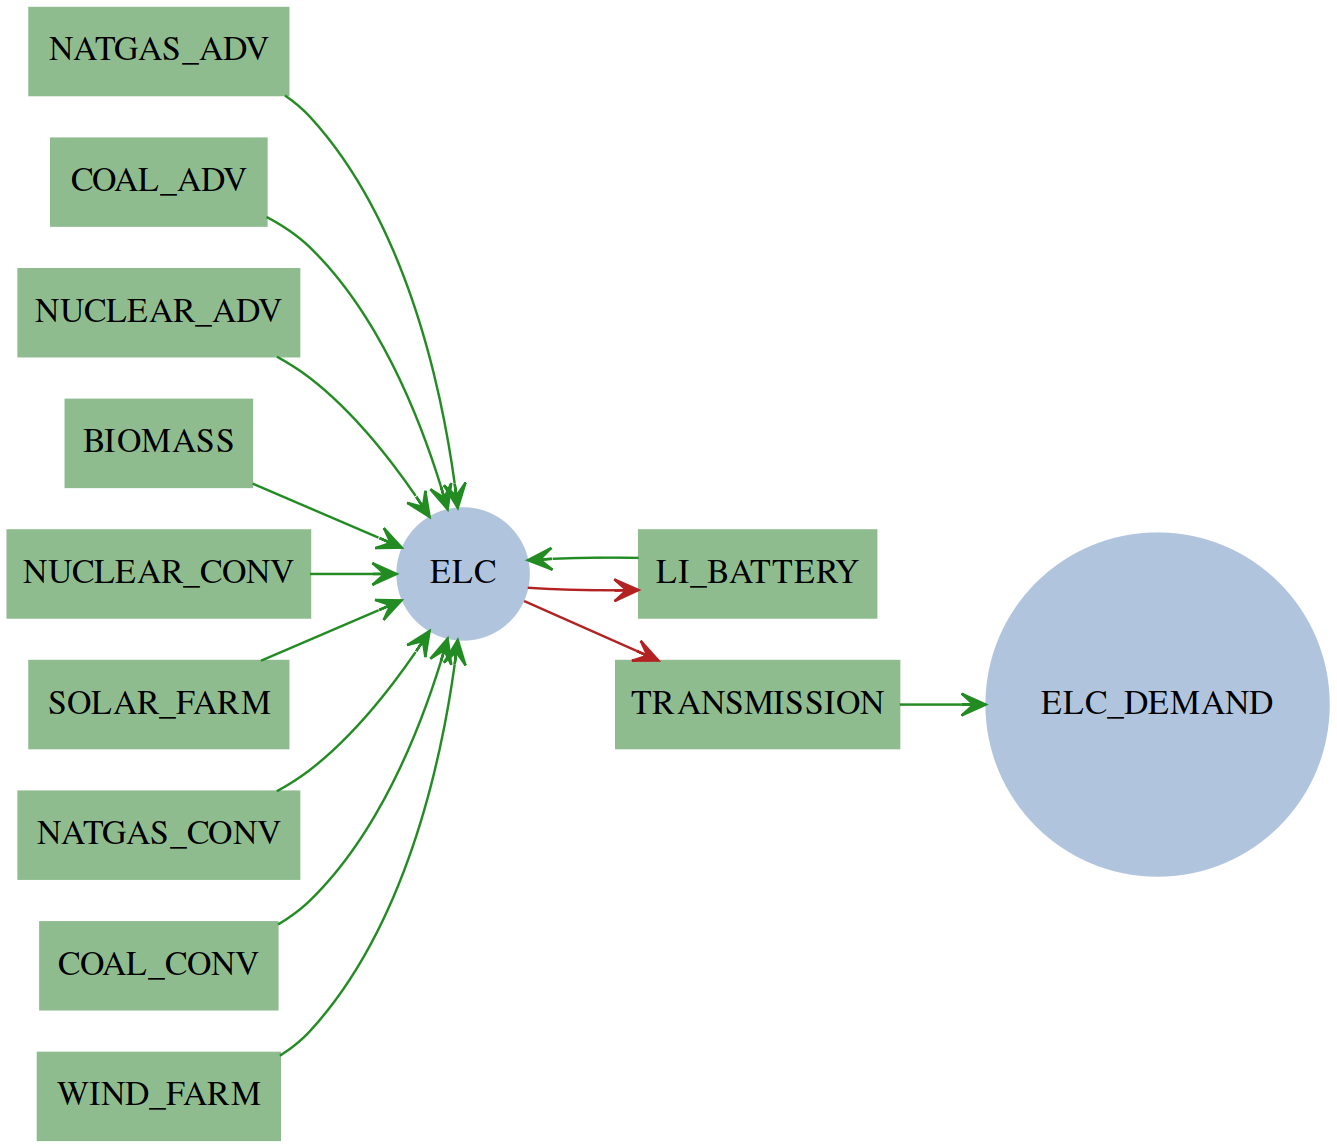
\includegraphics[width=0.6\columnwidth]{IL_system.png}
  \caption{The Illinois electricity grid modeled in \gls{temoa}.}
  \label{fig:ilsys}
\end{figure}

Figure \ref{fig:ilsys} shows the model topology of the Illinois system. There
are nine different electricity generating technologies and one storage option.
All generated electricity passes through a \texttt{TRANSMISSION} technology
to simulate electricity delivery. The Illinois model is spatially and topologically
simple since there are only ten distinct technologies, one region, and one
end-use commodity.

\subsection{Scenarios}
I consider four scenarios in the Illinois case study. Each scenario imposes forces
all carbon emissions from the electric sector to zero in 2030. This reflects Illinois'
current policy goal of 100\% clean electricity by 2030 \cite{office_of_governor_jb_pritzker_gov_2021}.
Further, each scenario adds a new constraint on nuclear energy in Illinois. Table
\ref{tab:il-scenarios} summarizes these constraints.

\begin{table}[H]
  \centering
  \caption{Summary of Illinois Case Study Scenarios}
  \label{tab:il-scenarios}
  \resizebox{\columnwidth}{!}{
  \begin{tabular}{lrrrr}
    \hline
    Name & Abbreviation & Time Horizon & Zero Emissions Year & Note\\
    \hline
    Least Cost & LC & 2025-2050 & 2030 & All technology options available\\
    Zero Advanced Nuclear  &ZAN &2025-2050 & 2030 & Advanced nuclear is explicitly disallowed\\
    Expensive Nuclear & XN & 2025-2050 & 2030 & Advanced nuclear capital costs doubled\\
    100\% Renewable & ZN &  2025-2050 &2030 & Nuclear energy is explicitly phased-out by 2050\\
    \hline
  \end{tabular}
  }
\end{table}

The ``zero advanced nuclear'' scenario simulates the Illinois moratorium on new nuclear
power plants. The moratorium stipulates that no new nuclear reactors may be
commissioned in Illinois unless the United States Government offers a means to
dispose of high level nuclear waste, or by specific approval from the Illinois
General Assembly \cite{shea_states_2021}. The ``expensive nuclear'' scenario
simulates the \textit{expectation} of significant cost overruns for \textit{every}
new reactor build. Finally, the ``100\% renewable'' scenario reflects current
Illinois policy to have 100\% renewable energy, as written in the \gls{ceja} bill
\cite{harmon_climate_2021}. This policy implicitly requires the retirement of
all existing Illinois nuclear plants.

\subsection{Model and Data}

\begin{table}[H]
  \centering
  \caption{Summary of Technologies and Parameters in the Illinois model}
  \label{tab:il-tech}
  \resizebox{\textwidth}{!}{
  % \begin{tabular}{llrrrrrrrrrrrr}
\toprule
        Name &                   Long Name & Efficiency &  Lifetime & Fixed Cost & Capital Cost & Variable Cost &        Sector & Baseload & Storage & Ramp Rate & CF& Primary Fuel &  CO$_2$ Rate \\
        &  & & [years] & [M\$/MW-year] & [M\$/MW] & [M\$/GWh] & & (Y/N) & [hours] & [\%] & [\%] &  & [MT/GWh] \\
\midrule
      ABBOTT &          Abbott Power Plant &       1.0$^\text{a}$ &        40 &                  0.0799 &                   0.613 &                  0.023 &         Steam &               Y &                      - &       - &                0.57 &  Natural Gas &                     0.000334 \\
   ABBOTT\_TB &        Abbott Steam Turbine &        0.4 &        40 &                     0.0 &                     0.0 &                    0.0 &      Electric &               N &                      - &       - &                 - &        Steam &                     - \\
 NUCLEAR\_THM &             Nuclear Reactor &       1.0$^\text{a}$ &        60 &                   0.121 &                    5.91 &                 0.0092 &         Steam &               N &                      - &      0.25 &                0.93 &      Uranium &                     - \\
  NUCLEAR\_TB &       Nuclear Steam Turbine &       0.33 &        60 &                     0.0 &                     0.0 &                    0.0 &      Electric &               N &                      - &       - &                 - &        Steam &                     - \\
     IMP\_ELC &        Imported Electricity &        1.0 &      1000 &                  0.0001 &                    0.49 &                 0.1161 &      Electric &               N &                      - &       - &                 - &          - &                     0.000850 \\
  SOLAR\_FARM &         Utility Scale Solar &        1.0 &        25 &                 0.07251 &                   1.274 &                    - &      Electric &               N &                      - &       - &              Varies &          - &                     - \\
   WIND\_FARM &     Utility Scale Wind Farm &        1.0 &        25 &                 0.04072 &                   1.754 &                    - &      Electric &               N &                      - &       - &              Varies &          - &                     - \\
  LI\_BATTERY &         Lithium-Ion Battery &        0.8 &        12 &                  0.0251 &                   1.608 &                    - &      Electric &               N &                      4.0 &       - &                 0.2 &          - &                     - \\
         CWS &        Chilled Water System &      1.467 &        40 &                0.000406 &                0.00189$^\text{a}$ &                 7.635$^\text{a}$ & Cooling &               N &                      - &       0.2 &               0.375 &  Electricity &                     - \\
  CW\_STORAGE &       Chilled Water Storage &       0.95 &       100 &                     - &                0.00178$^\text{a}$ &                    - & Cooling &               N &                      4.0 &     0.583 &                 0.5 &          - &                     - \\
TRANSMISSION & Electric Transmission Lines &        1.0 &      1000 &                     - &                     - &                    - &      Electric &               N &                      - &       - &                 - &          - &                     - \\
  STM\_TUNNEL &               Steam Tunnels &        1.0 &      1000 &                     - &                     - &                    - &         Steam &               N &                      - &       - &                 - &          - &                     - \\
    CW\_PIPES &         Chilled Water Pipes &        1.0 &      1000 &                     - &                     - &                    - & Cooling &               N &                      - &       - &                 - &          - &                     - \\
\bottomrule
\end{tabular}

  \begin{tabular}{llrrrrrrrrrrrr}
\toprule
        Name &                                          Long Name &  Efficiency &  Lifetime & Fixed Cost & Investment Cost& Variable Cost & Baseload & Storage Duration & Ramp Rate & Cap. Factor & Primary Fuel &  CO2 Rate & Source \\
        &  & [\%]  & [years] & [M\$/MW-year] & [M\$/MW] & [M\$/GWh] &(Y/N) & [hours] & [\%] & [\%] & & [MT/GWh] &  \\
\midrule
 NATGAS\_CONV &     Conventional   &         1.0 &        40 &                   0.011 &                    0.96 &                 0.0224 &               N &                      - &       - &                0.57 &  Natural Gas &                     0.000181 &   \cite{sargent__lundy_capital_2020}     \\
 &Combined Cycle&&&&&&&&&&&&\\
 &Natural Gas (NGCC)&&&&&&&&&&&&\\
  NATGAS\_ADV &            "Advanced"   &         1.0 &        40 &                      LC &                      LC &                 0.0275 &               N &                      - &       - &                0.57 &  Natural Gas &                     0.000018 &    \cite{nrel_2020_2020}    \\
  &NGCC with 90\%&&&&&&&&&&&&\\
  &carbon capture&&&&&&&&&&&&\\
NUCLEAR\_CONV &             Conventional   &         1.0 &        60 &                   0.178 &                    0.05 &                 0.0058 &               Y &                      - &       - &                0.93 &      Uranium &                     - &  \cite{desai_nuclear_2020,nei_status_2010}      \\
&Nuclear Reactor&&&&&&&&&&&&\\
&(PWR/BWR)&&&&&&&&&&&&\\
 NUCLEAR\_ADV &                "Advanced"   &         1.0 &        60 &                      0.119 &                      LC &                 0.0092 &               N &                      - &      0.25 &                0.93 &      Uranium &                     - &   \cite{nrel_2020_2020}     \\
 &Nuclear Reactor&&&&&&&&&&&&\\
 &(AP1000)&&&&&&&&&&&&\\
     BIOMASS &                            Dedicated Biomass  &         1.0 &        60 &                      0.123 &                      LC &                  0.047 &               Y &                      - &       - &                0.61 &      Biomass &                     - &       \cite{nrel_2020_2020} \\
     &Plant&&&&&&&&&&&&\\
  SOLAR\_FARM &                                Utility Scale Solar &         1.0 &        25 &                      LC &                      LC &                    - &               N &                      - &       - &          Mean: 0.17 &          - &                     - &       \cite{nrel_2020_2020} \\
   WIND\_FARM &                Utility Scale Wind Farm &         1.0 &        25 &                      LC &                      LC &                    - &               N &                      - &       - &         Mean: 0.347 &          - &                     - &     \cite{nrel_2020_2020}   \\
   &land-based&&&&&&&&&&&&\\
  LI\_BATTERY &                                Lithium-Ion Battery &         0.8 &        12 &                      LC &                      LC &                    - &               N &                      4.0 &       - &                 0.2 &  Electricity &                     - &     \cite{nrel_2020_2020}   \\
   COAL\_CONV &                      Conventional  &         1.0 &        40 &                  0.041 &                     1.0 &                0.02137 &               Y &                      - &       - &                0.54 &         Coal &                     0.000326 &    \cite{sargent__lundy_capital_2020}    \\
   &Coal-fired Plant&&&&&&&&&&&&\\
    COAL\_ADV & "Advanced"   &         1.0 &        40 &                      0.058 &                      LC &                0.03663 &               N &                      - &       0.5 &                0.54 &         Coal &                     0.000033 &    \cite{nrel_2020_2020}    \\
    &Coal-fired Plant&&&&&&&&&&&&\\
    &with 90\% carbon&&&&&&&&&&&&\\
    & capture&&&&&&&&&&&&\\
TRANSMISSION &                        Electric Transmission &         1.0 &      1000 &                     - &                     - &                    - &               N &                      - &       - &                 - &          - &                     - &        \\
\bottomrule
\end{tabular}

  } % end resize box
\end{table}

% \begin{figure}[H]
%   \centering
%   \resizebox{0.8\textwidth}{!}{%% Creator: Matplotlib, PGF backend
%%
%% To include the figure in your LaTeX document, write
%%   \input{<filename>.pgf}
%%
%% Make sure the required packages are loaded in your preamble
%%   \usepackage{pgf}
%%
%% Figures using additional raster images can only be included by \input if
%% they are in the same directory as the main LaTeX file. For loading figures
%% from other directories you can use the `import` package
%%   \usepackage{import}
%%
%% and then include the figures with
%%   \import{<path to file>}{<filename>.pgf}
%%
%% Matplotlib used the following preamble
%%
\begingroup%
\makeatletter%
\begin{pgfpicture}%
\pgfpathrectangle{\pgfpointorigin}{\pgfqpoint{10.024487in}{7.822276in}}%
\pgfusepath{use as bounding box, clip}%
\begin{pgfscope}%
\pgfsetbuttcap%
\pgfsetmiterjoin%
\definecolor{currentfill}{rgb}{1.000000,1.000000,1.000000}%
\pgfsetfillcolor{currentfill}%
\pgfsetlinewidth{0.000000pt}%
\definecolor{currentstroke}{rgb}{0.000000,0.000000,0.000000}%
\pgfsetstrokecolor{currentstroke}%
\pgfsetdash{}{0pt}%
\pgfpathmoveto{\pgfqpoint{0.000000in}{0.000000in}}%
\pgfpathlineto{\pgfqpoint{10.024487in}{0.000000in}}%
\pgfpathlineto{\pgfqpoint{10.024487in}{7.822276in}}%
\pgfpathlineto{\pgfqpoint{0.000000in}{7.822276in}}%
\pgfpathclose%
\pgfusepath{fill}%
\end{pgfscope}%
\begin{pgfscope}%
\pgfsetbuttcap%
\pgfsetmiterjoin%
\definecolor{currentfill}{rgb}{0.827451,0.827451,0.827451}%
\pgfsetfillcolor{currentfill}%
\pgfsetlinewidth{0.000000pt}%
\definecolor{currentstroke}{rgb}{0.000000,0.000000,0.000000}%
\pgfsetstrokecolor{currentstroke}%
\pgfsetstrokeopacity{0.000000}%
\pgfsetdash{}{0pt}%
\pgfpathmoveto{\pgfqpoint{0.590276in}{0.643904in}}%
\pgfpathlineto{\pgfqpoint{9.890276in}{0.643904in}}%
\pgfpathlineto{\pgfqpoint{9.890276in}{7.438904in}}%
\pgfpathlineto{\pgfqpoint{0.590276in}{7.438904in}}%
\pgfpathclose%
\pgfusepath{fill}%
\end{pgfscope}%
\begin{pgfscope}%
\pgfpathrectangle{\pgfqpoint{0.590276in}{0.643904in}}{\pgfqpoint{9.300000in}{6.795000in}}%
\pgfusepath{clip}%
\pgfsetrectcap%
\pgfsetroundjoin%
\pgfsetlinewidth{0.803000pt}%
\definecolor{currentstroke}{rgb}{1.000000,1.000000,1.000000}%
\pgfsetstrokecolor{currentstroke}%
\pgfsetdash{}{0pt}%
\pgfpathmoveto{\pgfqpoint{1.013003in}{0.643904in}}%
\pgfpathlineto{\pgfqpoint{1.013003in}{7.438904in}}%
\pgfusepath{stroke}%
\end{pgfscope}%
\begin{pgfscope}%
\pgfsetbuttcap%
\pgfsetroundjoin%
\definecolor{currentfill}{rgb}{0.000000,0.000000,0.000000}%
\pgfsetfillcolor{currentfill}%
\pgfsetlinewidth{0.803000pt}%
\definecolor{currentstroke}{rgb}{0.000000,0.000000,0.000000}%
\pgfsetstrokecolor{currentstroke}%
\pgfsetdash{}{0pt}%
\pgfsys@defobject{currentmarker}{\pgfqpoint{0.000000in}{-0.048611in}}{\pgfqpoint{0.000000in}{0.000000in}}{%
\pgfpathmoveto{\pgfqpoint{0.000000in}{0.000000in}}%
\pgfpathlineto{\pgfqpoint{0.000000in}{-0.048611in}}%
\pgfusepath{stroke,fill}%
}%
\begin{pgfscope}%
\pgfsys@transformshift{1.013003in}{0.643904in}%
\pgfsys@useobject{currentmarker}{}%
\end{pgfscope}%
\end{pgfscope}%
\begin{pgfscope}%
\definecolor{textcolor}{rgb}{0.000000,0.000000,0.000000}%
\pgfsetstrokecolor{textcolor}%
\pgfsetfillcolor{textcolor}%
\pgftext[x=1.013003in,y=0.546682in,,top]{\color{textcolor}\rmfamily\fontsize{14.000000}{16.800000}\selectfont 2000-01-01}%
\end{pgfscope}%
\begin{pgfscope}%
\pgfpathrectangle{\pgfqpoint{0.590276in}{0.643904in}}{\pgfqpoint{9.300000in}{6.795000in}}%
\pgfusepath{clip}%
\pgfsetrectcap%
\pgfsetroundjoin%
\pgfsetlinewidth{0.803000pt}%
\definecolor{currentstroke}{rgb}{1.000000,1.000000,1.000000}%
\pgfsetstrokecolor{currentstroke}%
\pgfsetdash{}{0pt}%
\pgfpathmoveto{\pgfqpoint{2.422094in}{0.643904in}}%
\pgfpathlineto{\pgfqpoint{2.422094in}{7.438904in}}%
\pgfusepath{stroke}%
\end{pgfscope}%
\begin{pgfscope}%
\pgfsetbuttcap%
\pgfsetroundjoin%
\definecolor{currentfill}{rgb}{0.000000,0.000000,0.000000}%
\pgfsetfillcolor{currentfill}%
\pgfsetlinewidth{0.803000pt}%
\definecolor{currentstroke}{rgb}{0.000000,0.000000,0.000000}%
\pgfsetstrokecolor{currentstroke}%
\pgfsetdash{}{0pt}%
\pgfsys@defobject{currentmarker}{\pgfqpoint{0.000000in}{-0.048611in}}{\pgfqpoint{0.000000in}{0.000000in}}{%
\pgfpathmoveto{\pgfqpoint{0.000000in}{0.000000in}}%
\pgfpathlineto{\pgfqpoint{0.000000in}{-0.048611in}}%
\pgfusepath{stroke,fill}%
}%
\begin{pgfscope}%
\pgfsys@transformshift{2.422094in}{0.643904in}%
\pgfsys@useobject{currentmarker}{}%
\end{pgfscope}%
\end{pgfscope}%
\begin{pgfscope}%
\definecolor{textcolor}{rgb}{0.000000,0.000000,0.000000}%
\pgfsetstrokecolor{textcolor}%
\pgfsetfillcolor{textcolor}%
\pgftext[x=2.422094in,y=0.546682in,,top]{\color{textcolor}\rmfamily\fontsize{14.000000}{16.800000}\selectfont 2010-01-01}%
\end{pgfscope}%
\begin{pgfscope}%
\pgfpathrectangle{\pgfqpoint{0.590276in}{0.643904in}}{\pgfqpoint{9.300000in}{6.795000in}}%
\pgfusepath{clip}%
\pgfsetrectcap%
\pgfsetroundjoin%
\pgfsetlinewidth{0.803000pt}%
\definecolor{currentstroke}{rgb}{1.000000,1.000000,1.000000}%
\pgfsetstrokecolor{currentstroke}%
\pgfsetdash{}{0pt}%
\pgfpathmoveto{\pgfqpoint{3.831185in}{0.643904in}}%
\pgfpathlineto{\pgfqpoint{3.831185in}{7.438904in}}%
\pgfusepath{stroke}%
\end{pgfscope}%
\begin{pgfscope}%
\pgfsetbuttcap%
\pgfsetroundjoin%
\definecolor{currentfill}{rgb}{0.000000,0.000000,0.000000}%
\pgfsetfillcolor{currentfill}%
\pgfsetlinewidth{0.803000pt}%
\definecolor{currentstroke}{rgb}{0.000000,0.000000,0.000000}%
\pgfsetstrokecolor{currentstroke}%
\pgfsetdash{}{0pt}%
\pgfsys@defobject{currentmarker}{\pgfqpoint{0.000000in}{-0.048611in}}{\pgfqpoint{0.000000in}{0.000000in}}{%
\pgfpathmoveto{\pgfqpoint{0.000000in}{0.000000in}}%
\pgfpathlineto{\pgfqpoint{0.000000in}{-0.048611in}}%
\pgfusepath{stroke,fill}%
}%
\begin{pgfscope}%
\pgfsys@transformshift{3.831185in}{0.643904in}%
\pgfsys@useobject{currentmarker}{}%
\end{pgfscope}%
\end{pgfscope}%
\begin{pgfscope}%
\definecolor{textcolor}{rgb}{0.000000,0.000000,0.000000}%
\pgfsetstrokecolor{textcolor}%
\pgfsetfillcolor{textcolor}%
\pgftext[x=3.831185in,y=0.546682in,,top]{\color{textcolor}\rmfamily\fontsize{14.000000}{16.800000}\selectfont 2020-01-01}%
\end{pgfscope}%
\begin{pgfscope}%
\pgfpathrectangle{\pgfqpoint{0.590276in}{0.643904in}}{\pgfqpoint{9.300000in}{6.795000in}}%
\pgfusepath{clip}%
\pgfsetrectcap%
\pgfsetroundjoin%
\pgfsetlinewidth{0.803000pt}%
\definecolor{currentstroke}{rgb}{1.000000,1.000000,1.000000}%
\pgfsetstrokecolor{currentstroke}%
\pgfsetdash{}{0pt}%
\pgfpathmoveto{\pgfqpoint{5.240276in}{0.643904in}}%
\pgfpathlineto{\pgfqpoint{5.240276in}{7.438904in}}%
\pgfusepath{stroke}%
\end{pgfscope}%
\begin{pgfscope}%
\pgfsetbuttcap%
\pgfsetroundjoin%
\definecolor{currentfill}{rgb}{0.000000,0.000000,0.000000}%
\pgfsetfillcolor{currentfill}%
\pgfsetlinewidth{0.803000pt}%
\definecolor{currentstroke}{rgb}{0.000000,0.000000,0.000000}%
\pgfsetstrokecolor{currentstroke}%
\pgfsetdash{}{0pt}%
\pgfsys@defobject{currentmarker}{\pgfqpoint{0.000000in}{-0.048611in}}{\pgfqpoint{0.000000in}{0.000000in}}{%
\pgfpathmoveto{\pgfqpoint{0.000000in}{0.000000in}}%
\pgfpathlineto{\pgfqpoint{0.000000in}{-0.048611in}}%
\pgfusepath{stroke,fill}%
}%
\begin{pgfscope}%
\pgfsys@transformshift{5.240276in}{0.643904in}%
\pgfsys@useobject{currentmarker}{}%
\end{pgfscope}%
\end{pgfscope}%
\begin{pgfscope}%
\definecolor{textcolor}{rgb}{0.000000,0.000000,0.000000}%
\pgfsetstrokecolor{textcolor}%
\pgfsetfillcolor{textcolor}%
\pgftext[x=5.240276in,y=0.546682in,,top]{\color{textcolor}\rmfamily\fontsize{14.000000}{16.800000}\selectfont 2030-01-01}%
\end{pgfscope}%
\begin{pgfscope}%
\pgfpathrectangle{\pgfqpoint{0.590276in}{0.643904in}}{\pgfqpoint{9.300000in}{6.795000in}}%
\pgfusepath{clip}%
\pgfsetrectcap%
\pgfsetroundjoin%
\pgfsetlinewidth{0.803000pt}%
\definecolor{currentstroke}{rgb}{1.000000,1.000000,1.000000}%
\pgfsetstrokecolor{currentstroke}%
\pgfsetdash{}{0pt}%
\pgfpathmoveto{\pgfqpoint{6.649367in}{0.643904in}}%
\pgfpathlineto{\pgfqpoint{6.649367in}{7.438904in}}%
\pgfusepath{stroke}%
\end{pgfscope}%
\begin{pgfscope}%
\pgfsetbuttcap%
\pgfsetroundjoin%
\definecolor{currentfill}{rgb}{0.000000,0.000000,0.000000}%
\pgfsetfillcolor{currentfill}%
\pgfsetlinewidth{0.803000pt}%
\definecolor{currentstroke}{rgb}{0.000000,0.000000,0.000000}%
\pgfsetstrokecolor{currentstroke}%
\pgfsetdash{}{0pt}%
\pgfsys@defobject{currentmarker}{\pgfqpoint{0.000000in}{-0.048611in}}{\pgfqpoint{0.000000in}{0.000000in}}{%
\pgfpathmoveto{\pgfqpoint{0.000000in}{0.000000in}}%
\pgfpathlineto{\pgfqpoint{0.000000in}{-0.048611in}}%
\pgfusepath{stroke,fill}%
}%
\begin{pgfscope}%
\pgfsys@transformshift{6.649367in}{0.643904in}%
\pgfsys@useobject{currentmarker}{}%
\end{pgfscope}%
\end{pgfscope}%
\begin{pgfscope}%
\definecolor{textcolor}{rgb}{0.000000,0.000000,0.000000}%
\pgfsetstrokecolor{textcolor}%
\pgfsetfillcolor{textcolor}%
\pgftext[x=6.649367in,y=0.546682in,,top]{\color{textcolor}\rmfamily\fontsize{14.000000}{16.800000}\selectfont 2040-01-01}%
\end{pgfscope}%
\begin{pgfscope}%
\pgfpathrectangle{\pgfqpoint{0.590276in}{0.643904in}}{\pgfqpoint{9.300000in}{6.795000in}}%
\pgfusepath{clip}%
\pgfsetrectcap%
\pgfsetroundjoin%
\pgfsetlinewidth{0.803000pt}%
\definecolor{currentstroke}{rgb}{1.000000,1.000000,1.000000}%
\pgfsetstrokecolor{currentstroke}%
\pgfsetdash{}{0pt}%
\pgfpathmoveto{\pgfqpoint{8.058458in}{0.643904in}}%
\pgfpathlineto{\pgfqpoint{8.058458in}{7.438904in}}%
\pgfusepath{stroke}%
\end{pgfscope}%
\begin{pgfscope}%
\pgfsetbuttcap%
\pgfsetroundjoin%
\definecolor{currentfill}{rgb}{0.000000,0.000000,0.000000}%
\pgfsetfillcolor{currentfill}%
\pgfsetlinewidth{0.803000pt}%
\definecolor{currentstroke}{rgb}{0.000000,0.000000,0.000000}%
\pgfsetstrokecolor{currentstroke}%
\pgfsetdash{}{0pt}%
\pgfsys@defobject{currentmarker}{\pgfqpoint{0.000000in}{-0.048611in}}{\pgfqpoint{0.000000in}{0.000000in}}{%
\pgfpathmoveto{\pgfqpoint{0.000000in}{0.000000in}}%
\pgfpathlineto{\pgfqpoint{0.000000in}{-0.048611in}}%
\pgfusepath{stroke,fill}%
}%
\begin{pgfscope}%
\pgfsys@transformshift{8.058458in}{0.643904in}%
\pgfsys@useobject{currentmarker}{}%
\end{pgfscope}%
\end{pgfscope}%
\begin{pgfscope}%
\definecolor{textcolor}{rgb}{0.000000,0.000000,0.000000}%
\pgfsetstrokecolor{textcolor}%
\pgfsetfillcolor{textcolor}%
\pgftext[x=8.058458in,y=0.546682in,,top]{\color{textcolor}\rmfamily\fontsize{14.000000}{16.800000}\selectfont 2050-01-01}%
\end{pgfscope}%
\begin{pgfscope}%
\pgfpathrectangle{\pgfqpoint{0.590276in}{0.643904in}}{\pgfqpoint{9.300000in}{6.795000in}}%
\pgfusepath{clip}%
\pgfsetrectcap%
\pgfsetroundjoin%
\pgfsetlinewidth{0.803000pt}%
\definecolor{currentstroke}{rgb}{1.000000,1.000000,1.000000}%
\pgfsetstrokecolor{currentstroke}%
\pgfsetdash{}{0pt}%
\pgfpathmoveto{\pgfqpoint{9.467549in}{0.643904in}}%
\pgfpathlineto{\pgfqpoint{9.467549in}{7.438904in}}%
\pgfusepath{stroke}%
\end{pgfscope}%
\begin{pgfscope}%
\pgfsetbuttcap%
\pgfsetroundjoin%
\definecolor{currentfill}{rgb}{0.000000,0.000000,0.000000}%
\pgfsetfillcolor{currentfill}%
\pgfsetlinewidth{0.803000pt}%
\definecolor{currentstroke}{rgb}{0.000000,0.000000,0.000000}%
\pgfsetstrokecolor{currentstroke}%
\pgfsetdash{}{0pt}%
\pgfsys@defobject{currentmarker}{\pgfqpoint{0.000000in}{-0.048611in}}{\pgfqpoint{0.000000in}{0.000000in}}{%
\pgfpathmoveto{\pgfqpoint{0.000000in}{0.000000in}}%
\pgfpathlineto{\pgfqpoint{0.000000in}{-0.048611in}}%
\pgfusepath{stroke,fill}%
}%
\begin{pgfscope}%
\pgfsys@transformshift{9.467549in}{0.643904in}%
\pgfsys@useobject{currentmarker}{}%
\end{pgfscope}%
\end{pgfscope}%
\begin{pgfscope}%
\definecolor{textcolor}{rgb}{0.000000,0.000000,0.000000}%
\pgfsetstrokecolor{textcolor}%
\pgfsetfillcolor{textcolor}%
\pgftext[x=9.467549in,y=0.546682in,,top]{\color{textcolor}\rmfamily\fontsize{14.000000}{16.800000}\selectfont 2060-01-01}%
\end{pgfscope}%
\begin{pgfscope}%
\pgfpathrectangle{\pgfqpoint{0.590276in}{0.643904in}}{\pgfqpoint{9.300000in}{6.795000in}}%
\pgfusepath{clip}%
\pgfsetbuttcap%
\pgfsetroundjoin%
\pgfsetlinewidth{0.501875pt}%
\definecolor{currentstroke}{rgb}{1.000000,1.000000,1.000000}%
\pgfsetstrokecolor{currentstroke}%
\pgfsetdash{{1.850000pt}{0.800000pt}}{0.000000pt}%
\pgfpathmoveto{\pgfqpoint{0.731185in}{0.643904in}}%
\pgfpathlineto{\pgfqpoint{0.731185in}{7.438904in}}%
\pgfusepath{stroke}%
\end{pgfscope}%
\begin{pgfscope}%
\pgfsetbuttcap%
\pgfsetroundjoin%
\definecolor{currentfill}{rgb}{0.000000,0.000000,0.000000}%
\pgfsetfillcolor{currentfill}%
\pgfsetlinewidth{0.602250pt}%
\definecolor{currentstroke}{rgb}{0.000000,0.000000,0.000000}%
\pgfsetstrokecolor{currentstroke}%
\pgfsetdash{}{0pt}%
\pgfsys@defobject{currentmarker}{\pgfqpoint{0.000000in}{-0.027778in}}{\pgfqpoint{0.000000in}{0.000000in}}{%
\pgfpathmoveto{\pgfqpoint{0.000000in}{0.000000in}}%
\pgfpathlineto{\pgfqpoint{0.000000in}{-0.027778in}}%
\pgfusepath{stroke,fill}%
}%
\begin{pgfscope}%
\pgfsys@transformshift{0.731185in}{0.643904in}%
\pgfsys@useobject{currentmarker}{}%
\end{pgfscope}%
\end{pgfscope}%
\begin{pgfscope}%
\pgfpathrectangle{\pgfqpoint{0.590276in}{0.643904in}}{\pgfqpoint{9.300000in}{6.795000in}}%
\pgfusepath{clip}%
\pgfsetbuttcap%
\pgfsetroundjoin%
\pgfsetlinewidth{0.501875pt}%
\definecolor{currentstroke}{rgb}{1.000000,1.000000,1.000000}%
\pgfsetstrokecolor{currentstroke}%
\pgfsetdash{{1.850000pt}{0.800000pt}}{0.000000pt}%
\pgfpathmoveto{\pgfqpoint{1.294822in}{0.643904in}}%
\pgfpathlineto{\pgfqpoint{1.294822in}{7.438904in}}%
\pgfusepath{stroke}%
\end{pgfscope}%
\begin{pgfscope}%
\pgfsetbuttcap%
\pgfsetroundjoin%
\definecolor{currentfill}{rgb}{0.000000,0.000000,0.000000}%
\pgfsetfillcolor{currentfill}%
\pgfsetlinewidth{0.602250pt}%
\definecolor{currentstroke}{rgb}{0.000000,0.000000,0.000000}%
\pgfsetstrokecolor{currentstroke}%
\pgfsetdash{}{0pt}%
\pgfsys@defobject{currentmarker}{\pgfqpoint{0.000000in}{-0.027778in}}{\pgfqpoint{0.000000in}{0.000000in}}{%
\pgfpathmoveto{\pgfqpoint{0.000000in}{0.000000in}}%
\pgfpathlineto{\pgfqpoint{0.000000in}{-0.027778in}}%
\pgfusepath{stroke,fill}%
}%
\begin{pgfscope}%
\pgfsys@transformshift{1.294822in}{0.643904in}%
\pgfsys@useobject{currentmarker}{}%
\end{pgfscope}%
\end{pgfscope}%
\begin{pgfscope}%
\pgfpathrectangle{\pgfqpoint{0.590276in}{0.643904in}}{\pgfqpoint{9.300000in}{6.795000in}}%
\pgfusepath{clip}%
\pgfsetbuttcap%
\pgfsetroundjoin%
\pgfsetlinewidth{0.501875pt}%
\definecolor{currentstroke}{rgb}{1.000000,1.000000,1.000000}%
\pgfsetstrokecolor{currentstroke}%
\pgfsetdash{{1.850000pt}{0.800000pt}}{0.000000pt}%
\pgfpathmoveto{\pgfqpoint{1.576640in}{0.643904in}}%
\pgfpathlineto{\pgfqpoint{1.576640in}{7.438904in}}%
\pgfusepath{stroke}%
\end{pgfscope}%
\begin{pgfscope}%
\pgfsetbuttcap%
\pgfsetroundjoin%
\definecolor{currentfill}{rgb}{0.000000,0.000000,0.000000}%
\pgfsetfillcolor{currentfill}%
\pgfsetlinewidth{0.602250pt}%
\definecolor{currentstroke}{rgb}{0.000000,0.000000,0.000000}%
\pgfsetstrokecolor{currentstroke}%
\pgfsetdash{}{0pt}%
\pgfsys@defobject{currentmarker}{\pgfqpoint{0.000000in}{-0.027778in}}{\pgfqpoint{0.000000in}{0.000000in}}{%
\pgfpathmoveto{\pgfqpoint{0.000000in}{0.000000in}}%
\pgfpathlineto{\pgfqpoint{0.000000in}{-0.027778in}}%
\pgfusepath{stroke,fill}%
}%
\begin{pgfscope}%
\pgfsys@transformshift{1.576640in}{0.643904in}%
\pgfsys@useobject{currentmarker}{}%
\end{pgfscope}%
\end{pgfscope}%
\begin{pgfscope}%
\pgfpathrectangle{\pgfqpoint{0.590276in}{0.643904in}}{\pgfqpoint{9.300000in}{6.795000in}}%
\pgfusepath{clip}%
\pgfsetbuttcap%
\pgfsetroundjoin%
\pgfsetlinewidth{0.501875pt}%
\definecolor{currentstroke}{rgb}{1.000000,1.000000,1.000000}%
\pgfsetstrokecolor{currentstroke}%
\pgfsetdash{{1.850000pt}{0.800000pt}}{0.000000pt}%
\pgfpathmoveto{\pgfqpoint{1.858458in}{0.643904in}}%
\pgfpathlineto{\pgfqpoint{1.858458in}{7.438904in}}%
\pgfusepath{stroke}%
\end{pgfscope}%
\begin{pgfscope}%
\pgfsetbuttcap%
\pgfsetroundjoin%
\definecolor{currentfill}{rgb}{0.000000,0.000000,0.000000}%
\pgfsetfillcolor{currentfill}%
\pgfsetlinewidth{0.602250pt}%
\definecolor{currentstroke}{rgb}{0.000000,0.000000,0.000000}%
\pgfsetstrokecolor{currentstroke}%
\pgfsetdash{}{0pt}%
\pgfsys@defobject{currentmarker}{\pgfqpoint{0.000000in}{-0.027778in}}{\pgfqpoint{0.000000in}{0.000000in}}{%
\pgfpathmoveto{\pgfqpoint{0.000000in}{0.000000in}}%
\pgfpathlineto{\pgfqpoint{0.000000in}{-0.027778in}}%
\pgfusepath{stroke,fill}%
}%
\begin{pgfscope}%
\pgfsys@transformshift{1.858458in}{0.643904in}%
\pgfsys@useobject{currentmarker}{}%
\end{pgfscope}%
\end{pgfscope}%
\begin{pgfscope}%
\pgfpathrectangle{\pgfqpoint{0.590276in}{0.643904in}}{\pgfqpoint{9.300000in}{6.795000in}}%
\pgfusepath{clip}%
\pgfsetbuttcap%
\pgfsetroundjoin%
\pgfsetlinewidth{0.501875pt}%
\definecolor{currentstroke}{rgb}{1.000000,1.000000,1.000000}%
\pgfsetstrokecolor{currentstroke}%
\pgfsetdash{{1.850000pt}{0.800000pt}}{0.000000pt}%
\pgfpathmoveto{\pgfqpoint{2.140276in}{0.643904in}}%
\pgfpathlineto{\pgfqpoint{2.140276in}{7.438904in}}%
\pgfusepath{stroke}%
\end{pgfscope}%
\begin{pgfscope}%
\pgfsetbuttcap%
\pgfsetroundjoin%
\definecolor{currentfill}{rgb}{0.000000,0.000000,0.000000}%
\pgfsetfillcolor{currentfill}%
\pgfsetlinewidth{0.602250pt}%
\definecolor{currentstroke}{rgb}{0.000000,0.000000,0.000000}%
\pgfsetstrokecolor{currentstroke}%
\pgfsetdash{}{0pt}%
\pgfsys@defobject{currentmarker}{\pgfqpoint{0.000000in}{-0.027778in}}{\pgfqpoint{0.000000in}{0.000000in}}{%
\pgfpathmoveto{\pgfqpoint{0.000000in}{0.000000in}}%
\pgfpathlineto{\pgfqpoint{0.000000in}{-0.027778in}}%
\pgfusepath{stroke,fill}%
}%
\begin{pgfscope}%
\pgfsys@transformshift{2.140276in}{0.643904in}%
\pgfsys@useobject{currentmarker}{}%
\end{pgfscope}%
\end{pgfscope}%
\begin{pgfscope}%
\pgfpathrectangle{\pgfqpoint{0.590276in}{0.643904in}}{\pgfqpoint{9.300000in}{6.795000in}}%
\pgfusepath{clip}%
\pgfsetbuttcap%
\pgfsetroundjoin%
\pgfsetlinewidth{0.501875pt}%
\definecolor{currentstroke}{rgb}{1.000000,1.000000,1.000000}%
\pgfsetstrokecolor{currentstroke}%
\pgfsetdash{{1.850000pt}{0.800000pt}}{0.000000pt}%
\pgfpathmoveto{\pgfqpoint{2.703912in}{0.643904in}}%
\pgfpathlineto{\pgfqpoint{2.703912in}{7.438904in}}%
\pgfusepath{stroke}%
\end{pgfscope}%
\begin{pgfscope}%
\pgfsetbuttcap%
\pgfsetroundjoin%
\definecolor{currentfill}{rgb}{0.000000,0.000000,0.000000}%
\pgfsetfillcolor{currentfill}%
\pgfsetlinewidth{0.602250pt}%
\definecolor{currentstroke}{rgb}{0.000000,0.000000,0.000000}%
\pgfsetstrokecolor{currentstroke}%
\pgfsetdash{}{0pt}%
\pgfsys@defobject{currentmarker}{\pgfqpoint{0.000000in}{-0.027778in}}{\pgfqpoint{0.000000in}{0.000000in}}{%
\pgfpathmoveto{\pgfqpoint{0.000000in}{0.000000in}}%
\pgfpathlineto{\pgfqpoint{0.000000in}{-0.027778in}}%
\pgfusepath{stroke,fill}%
}%
\begin{pgfscope}%
\pgfsys@transformshift{2.703912in}{0.643904in}%
\pgfsys@useobject{currentmarker}{}%
\end{pgfscope}%
\end{pgfscope}%
\begin{pgfscope}%
\pgfpathrectangle{\pgfqpoint{0.590276in}{0.643904in}}{\pgfqpoint{9.300000in}{6.795000in}}%
\pgfusepath{clip}%
\pgfsetbuttcap%
\pgfsetroundjoin%
\pgfsetlinewidth{0.501875pt}%
\definecolor{currentstroke}{rgb}{1.000000,1.000000,1.000000}%
\pgfsetstrokecolor{currentstroke}%
\pgfsetdash{{1.850000pt}{0.800000pt}}{0.000000pt}%
\pgfpathmoveto{\pgfqpoint{2.985731in}{0.643904in}}%
\pgfpathlineto{\pgfqpoint{2.985731in}{7.438904in}}%
\pgfusepath{stroke}%
\end{pgfscope}%
\begin{pgfscope}%
\pgfsetbuttcap%
\pgfsetroundjoin%
\definecolor{currentfill}{rgb}{0.000000,0.000000,0.000000}%
\pgfsetfillcolor{currentfill}%
\pgfsetlinewidth{0.602250pt}%
\definecolor{currentstroke}{rgb}{0.000000,0.000000,0.000000}%
\pgfsetstrokecolor{currentstroke}%
\pgfsetdash{}{0pt}%
\pgfsys@defobject{currentmarker}{\pgfqpoint{0.000000in}{-0.027778in}}{\pgfqpoint{0.000000in}{0.000000in}}{%
\pgfpathmoveto{\pgfqpoint{0.000000in}{0.000000in}}%
\pgfpathlineto{\pgfqpoint{0.000000in}{-0.027778in}}%
\pgfusepath{stroke,fill}%
}%
\begin{pgfscope}%
\pgfsys@transformshift{2.985731in}{0.643904in}%
\pgfsys@useobject{currentmarker}{}%
\end{pgfscope}%
\end{pgfscope}%
\begin{pgfscope}%
\pgfpathrectangle{\pgfqpoint{0.590276in}{0.643904in}}{\pgfqpoint{9.300000in}{6.795000in}}%
\pgfusepath{clip}%
\pgfsetbuttcap%
\pgfsetroundjoin%
\pgfsetlinewidth{0.501875pt}%
\definecolor{currentstroke}{rgb}{1.000000,1.000000,1.000000}%
\pgfsetstrokecolor{currentstroke}%
\pgfsetdash{{1.850000pt}{0.800000pt}}{0.000000pt}%
\pgfpathmoveto{\pgfqpoint{3.267549in}{0.643904in}}%
\pgfpathlineto{\pgfqpoint{3.267549in}{7.438904in}}%
\pgfusepath{stroke}%
\end{pgfscope}%
\begin{pgfscope}%
\pgfsetbuttcap%
\pgfsetroundjoin%
\definecolor{currentfill}{rgb}{0.000000,0.000000,0.000000}%
\pgfsetfillcolor{currentfill}%
\pgfsetlinewidth{0.602250pt}%
\definecolor{currentstroke}{rgb}{0.000000,0.000000,0.000000}%
\pgfsetstrokecolor{currentstroke}%
\pgfsetdash{}{0pt}%
\pgfsys@defobject{currentmarker}{\pgfqpoint{0.000000in}{-0.027778in}}{\pgfqpoint{0.000000in}{0.000000in}}{%
\pgfpathmoveto{\pgfqpoint{0.000000in}{0.000000in}}%
\pgfpathlineto{\pgfqpoint{0.000000in}{-0.027778in}}%
\pgfusepath{stroke,fill}%
}%
\begin{pgfscope}%
\pgfsys@transformshift{3.267549in}{0.643904in}%
\pgfsys@useobject{currentmarker}{}%
\end{pgfscope}%
\end{pgfscope}%
\begin{pgfscope}%
\pgfpathrectangle{\pgfqpoint{0.590276in}{0.643904in}}{\pgfqpoint{9.300000in}{6.795000in}}%
\pgfusepath{clip}%
\pgfsetbuttcap%
\pgfsetroundjoin%
\pgfsetlinewidth{0.501875pt}%
\definecolor{currentstroke}{rgb}{1.000000,1.000000,1.000000}%
\pgfsetstrokecolor{currentstroke}%
\pgfsetdash{{1.850000pt}{0.800000pt}}{0.000000pt}%
\pgfpathmoveto{\pgfqpoint{3.549367in}{0.643904in}}%
\pgfpathlineto{\pgfqpoint{3.549367in}{7.438904in}}%
\pgfusepath{stroke}%
\end{pgfscope}%
\begin{pgfscope}%
\pgfsetbuttcap%
\pgfsetroundjoin%
\definecolor{currentfill}{rgb}{0.000000,0.000000,0.000000}%
\pgfsetfillcolor{currentfill}%
\pgfsetlinewidth{0.602250pt}%
\definecolor{currentstroke}{rgb}{0.000000,0.000000,0.000000}%
\pgfsetstrokecolor{currentstroke}%
\pgfsetdash{}{0pt}%
\pgfsys@defobject{currentmarker}{\pgfqpoint{0.000000in}{-0.027778in}}{\pgfqpoint{0.000000in}{0.000000in}}{%
\pgfpathmoveto{\pgfqpoint{0.000000in}{0.000000in}}%
\pgfpathlineto{\pgfqpoint{0.000000in}{-0.027778in}}%
\pgfusepath{stroke,fill}%
}%
\begin{pgfscope}%
\pgfsys@transformshift{3.549367in}{0.643904in}%
\pgfsys@useobject{currentmarker}{}%
\end{pgfscope}%
\end{pgfscope}%
\begin{pgfscope}%
\pgfpathrectangle{\pgfqpoint{0.590276in}{0.643904in}}{\pgfqpoint{9.300000in}{6.795000in}}%
\pgfusepath{clip}%
\pgfsetbuttcap%
\pgfsetroundjoin%
\pgfsetlinewidth{0.501875pt}%
\definecolor{currentstroke}{rgb}{1.000000,1.000000,1.000000}%
\pgfsetstrokecolor{currentstroke}%
\pgfsetdash{{1.850000pt}{0.800000pt}}{0.000000pt}%
\pgfpathmoveto{\pgfqpoint{4.113003in}{0.643904in}}%
\pgfpathlineto{\pgfqpoint{4.113003in}{7.438904in}}%
\pgfusepath{stroke}%
\end{pgfscope}%
\begin{pgfscope}%
\pgfsetbuttcap%
\pgfsetroundjoin%
\definecolor{currentfill}{rgb}{0.000000,0.000000,0.000000}%
\pgfsetfillcolor{currentfill}%
\pgfsetlinewidth{0.602250pt}%
\definecolor{currentstroke}{rgb}{0.000000,0.000000,0.000000}%
\pgfsetstrokecolor{currentstroke}%
\pgfsetdash{}{0pt}%
\pgfsys@defobject{currentmarker}{\pgfqpoint{0.000000in}{-0.027778in}}{\pgfqpoint{0.000000in}{0.000000in}}{%
\pgfpathmoveto{\pgfqpoint{0.000000in}{0.000000in}}%
\pgfpathlineto{\pgfqpoint{0.000000in}{-0.027778in}}%
\pgfusepath{stroke,fill}%
}%
\begin{pgfscope}%
\pgfsys@transformshift{4.113003in}{0.643904in}%
\pgfsys@useobject{currentmarker}{}%
\end{pgfscope}%
\end{pgfscope}%
\begin{pgfscope}%
\pgfpathrectangle{\pgfqpoint{0.590276in}{0.643904in}}{\pgfqpoint{9.300000in}{6.795000in}}%
\pgfusepath{clip}%
\pgfsetbuttcap%
\pgfsetroundjoin%
\pgfsetlinewidth{0.501875pt}%
\definecolor{currentstroke}{rgb}{1.000000,1.000000,1.000000}%
\pgfsetstrokecolor{currentstroke}%
\pgfsetdash{{1.850000pt}{0.800000pt}}{0.000000pt}%
\pgfpathmoveto{\pgfqpoint{4.394822in}{0.643904in}}%
\pgfpathlineto{\pgfqpoint{4.394822in}{7.438904in}}%
\pgfusepath{stroke}%
\end{pgfscope}%
\begin{pgfscope}%
\pgfsetbuttcap%
\pgfsetroundjoin%
\definecolor{currentfill}{rgb}{0.000000,0.000000,0.000000}%
\pgfsetfillcolor{currentfill}%
\pgfsetlinewidth{0.602250pt}%
\definecolor{currentstroke}{rgb}{0.000000,0.000000,0.000000}%
\pgfsetstrokecolor{currentstroke}%
\pgfsetdash{}{0pt}%
\pgfsys@defobject{currentmarker}{\pgfqpoint{0.000000in}{-0.027778in}}{\pgfqpoint{0.000000in}{0.000000in}}{%
\pgfpathmoveto{\pgfqpoint{0.000000in}{0.000000in}}%
\pgfpathlineto{\pgfqpoint{0.000000in}{-0.027778in}}%
\pgfusepath{stroke,fill}%
}%
\begin{pgfscope}%
\pgfsys@transformshift{4.394822in}{0.643904in}%
\pgfsys@useobject{currentmarker}{}%
\end{pgfscope}%
\end{pgfscope}%
\begin{pgfscope}%
\pgfpathrectangle{\pgfqpoint{0.590276in}{0.643904in}}{\pgfqpoint{9.300000in}{6.795000in}}%
\pgfusepath{clip}%
\pgfsetbuttcap%
\pgfsetroundjoin%
\pgfsetlinewidth{0.501875pt}%
\definecolor{currentstroke}{rgb}{1.000000,1.000000,1.000000}%
\pgfsetstrokecolor{currentstroke}%
\pgfsetdash{{1.850000pt}{0.800000pt}}{0.000000pt}%
\pgfpathmoveto{\pgfqpoint{4.676640in}{0.643904in}}%
\pgfpathlineto{\pgfqpoint{4.676640in}{7.438904in}}%
\pgfusepath{stroke}%
\end{pgfscope}%
\begin{pgfscope}%
\pgfsetbuttcap%
\pgfsetroundjoin%
\definecolor{currentfill}{rgb}{0.000000,0.000000,0.000000}%
\pgfsetfillcolor{currentfill}%
\pgfsetlinewidth{0.602250pt}%
\definecolor{currentstroke}{rgb}{0.000000,0.000000,0.000000}%
\pgfsetstrokecolor{currentstroke}%
\pgfsetdash{}{0pt}%
\pgfsys@defobject{currentmarker}{\pgfqpoint{0.000000in}{-0.027778in}}{\pgfqpoint{0.000000in}{0.000000in}}{%
\pgfpathmoveto{\pgfqpoint{0.000000in}{0.000000in}}%
\pgfpathlineto{\pgfqpoint{0.000000in}{-0.027778in}}%
\pgfusepath{stroke,fill}%
}%
\begin{pgfscope}%
\pgfsys@transformshift{4.676640in}{0.643904in}%
\pgfsys@useobject{currentmarker}{}%
\end{pgfscope}%
\end{pgfscope}%
\begin{pgfscope}%
\pgfpathrectangle{\pgfqpoint{0.590276in}{0.643904in}}{\pgfqpoint{9.300000in}{6.795000in}}%
\pgfusepath{clip}%
\pgfsetbuttcap%
\pgfsetroundjoin%
\pgfsetlinewidth{0.501875pt}%
\definecolor{currentstroke}{rgb}{1.000000,1.000000,1.000000}%
\pgfsetstrokecolor{currentstroke}%
\pgfsetdash{{1.850000pt}{0.800000pt}}{0.000000pt}%
\pgfpathmoveto{\pgfqpoint{4.958458in}{0.643904in}}%
\pgfpathlineto{\pgfqpoint{4.958458in}{7.438904in}}%
\pgfusepath{stroke}%
\end{pgfscope}%
\begin{pgfscope}%
\pgfsetbuttcap%
\pgfsetroundjoin%
\definecolor{currentfill}{rgb}{0.000000,0.000000,0.000000}%
\pgfsetfillcolor{currentfill}%
\pgfsetlinewidth{0.602250pt}%
\definecolor{currentstroke}{rgb}{0.000000,0.000000,0.000000}%
\pgfsetstrokecolor{currentstroke}%
\pgfsetdash{}{0pt}%
\pgfsys@defobject{currentmarker}{\pgfqpoint{0.000000in}{-0.027778in}}{\pgfqpoint{0.000000in}{0.000000in}}{%
\pgfpathmoveto{\pgfqpoint{0.000000in}{0.000000in}}%
\pgfpathlineto{\pgfqpoint{0.000000in}{-0.027778in}}%
\pgfusepath{stroke,fill}%
}%
\begin{pgfscope}%
\pgfsys@transformshift{4.958458in}{0.643904in}%
\pgfsys@useobject{currentmarker}{}%
\end{pgfscope}%
\end{pgfscope}%
\begin{pgfscope}%
\pgfpathrectangle{\pgfqpoint{0.590276in}{0.643904in}}{\pgfqpoint{9.300000in}{6.795000in}}%
\pgfusepath{clip}%
\pgfsetbuttcap%
\pgfsetroundjoin%
\pgfsetlinewidth{0.501875pt}%
\definecolor{currentstroke}{rgb}{1.000000,1.000000,1.000000}%
\pgfsetstrokecolor{currentstroke}%
\pgfsetdash{{1.850000pt}{0.800000pt}}{0.000000pt}%
\pgfpathmoveto{\pgfqpoint{5.522094in}{0.643904in}}%
\pgfpathlineto{\pgfqpoint{5.522094in}{7.438904in}}%
\pgfusepath{stroke}%
\end{pgfscope}%
\begin{pgfscope}%
\pgfsetbuttcap%
\pgfsetroundjoin%
\definecolor{currentfill}{rgb}{0.000000,0.000000,0.000000}%
\pgfsetfillcolor{currentfill}%
\pgfsetlinewidth{0.602250pt}%
\definecolor{currentstroke}{rgb}{0.000000,0.000000,0.000000}%
\pgfsetstrokecolor{currentstroke}%
\pgfsetdash{}{0pt}%
\pgfsys@defobject{currentmarker}{\pgfqpoint{0.000000in}{-0.027778in}}{\pgfqpoint{0.000000in}{0.000000in}}{%
\pgfpathmoveto{\pgfqpoint{0.000000in}{0.000000in}}%
\pgfpathlineto{\pgfqpoint{0.000000in}{-0.027778in}}%
\pgfusepath{stroke,fill}%
}%
\begin{pgfscope}%
\pgfsys@transformshift{5.522094in}{0.643904in}%
\pgfsys@useobject{currentmarker}{}%
\end{pgfscope}%
\end{pgfscope}%
\begin{pgfscope}%
\pgfpathrectangle{\pgfqpoint{0.590276in}{0.643904in}}{\pgfqpoint{9.300000in}{6.795000in}}%
\pgfusepath{clip}%
\pgfsetbuttcap%
\pgfsetroundjoin%
\pgfsetlinewidth{0.501875pt}%
\definecolor{currentstroke}{rgb}{1.000000,1.000000,1.000000}%
\pgfsetstrokecolor{currentstroke}%
\pgfsetdash{{1.850000pt}{0.800000pt}}{0.000000pt}%
\pgfpathmoveto{\pgfqpoint{5.803912in}{0.643904in}}%
\pgfpathlineto{\pgfqpoint{5.803912in}{7.438904in}}%
\pgfusepath{stroke}%
\end{pgfscope}%
\begin{pgfscope}%
\pgfsetbuttcap%
\pgfsetroundjoin%
\definecolor{currentfill}{rgb}{0.000000,0.000000,0.000000}%
\pgfsetfillcolor{currentfill}%
\pgfsetlinewidth{0.602250pt}%
\definecolor{currentstroke}{rgb}{0.000000,0.000000,0.000000}%
\pgfsetstrokecolor{currentstroke}%
\pgfsetdash{}{0pt}%
\pgfsys@defobject{currentmarker}{\pgfqpoint{0.000000in}{-0.027778in}}{\pgfqpoint{0.000000in}{0.000000in}}{%
\pgfpathmoveto{\pgfqpoint{0.000000in}{0.000000in}}%
\pgfpathlineto{\pgfqpoint{0.000000in}{-0.027778in}}%
\pgfusepath{stroke,fill}%
}%
\begin{pgfscope}%
\pgfsys@transformshift{5.803912in}{0.643904in}%
\pgfsys@useobject{currentmarker}{}%
\end{pgfscope}%
\end{pgfscope}%
\begin{pgfscope}%
\pgfpathrectangle{\pgfqpoint{0.590276in}{0.643904in}}{\pgfqpoint{9.300000in}{6.795000in}}%
\pgfusepath{clip}%
\pgfsetbuttcap%
\pgfsetroundjoin%
\pgfsetlinewidth{0.501875pt}%
\definecolor{currentstroke}{rgb}{1.000000,1.000000,1.000000}%
\pgfsetstrokecolor{currentstroke}%
\pgfsetdash{{1.850000pt}{0.800000pt}}{0.000000pt}%
\pgfpathmoveto{\pgfqpoint{6.085731in}{0.643904in}}%
\pgfpathlineto{\pgfqpoint{6.085731in}{7.438904in}}%
\pgfusepath{stroke}%
\end{pgfscope}%
\begin{pgfscope}%
\pgfsetbuttcap%
\pgfsetroundjoin%
\definecolor{currentfill}{rgb}{0.000000,0.000000,0.000000}%
\pgfsetfillcolor{currentfill}%
\pgfsetlinewidth{0.602250pt}%
\definecolor{currentstroke}{rgb}{0.000000,0.000000,0.000000}%
\pgfsetstrokecolor{currentstroke}%
\pgfsetdash{}{0pt}%
\pgfsys@defobject{currentmarker}{\pgfqpoint{0.000000in}{-0.027778in}}{\pgfqpoint{0.000000in}{0.000000in}}{%
\pgfpathmoveto{\pgfqpoint{0.000000in}{0.000000in}}%
\pgfpathlineto{\pgfqpoint{0.000000in}{-0.027778in}}%
\pgfusepath{stroke,fill}%
}%
\begin{pgfscope}%
\pgfsys@transformshift{6.085731in}{0.643904in}%
\pgfsys@useobject{currentmarker}{}%
\end{pgfscope}%
\end{pgfscope}%
\begin{pgfscope}%
\pgfpathrectangle{\pgfqpoint{0.590276in}{0.643904in}}{\pgfqpoint{9.300000in}{6.795000in}}%
\pgfusepath{clip}%
\pgfsetbuttcap%
\pgfsetroundjoin%
\pgfsetlinewidth{0.501875pt}%
\definecolor{currentstroke}{rgb}{1.000000,1.000000,1.000000}%
\pgfsetstrokecolor{currentstroke}%
\pgfsetdash{{1.850000pt}{0.800000pt}}{0.000000pt}%
\pgfpathmoveto{\pgfqpoint{6.367549in}{0.643904in}}%
\pgfpathlineto{\pgfqpoint{6.367549in}{7.438904in}}%
\pgfusepath{stroke}%
\end{pgfscope}%
\begin{pgfscope}%
\pgfsetbuttcap%
\pgfsetroundjoin%
\definecolor{currentfill}{rgb}{0.000000,0.000000,0.000000}%
\pgfsetfillcolor{currentfill}%
\pgfsetlinewidth{0.602250pt}%
\definecolor{currentstroke}{rgb}{0.000000,0.000000,0.000000}%
\pgfsetstrokecolor{currentstroke}%
\pgfsetdash{}{0pt}%
\pgfsys@defobject{currentmarker}{\pgfqpoint{0.000000in}{-0.027778in}}{\pgfqpoint{0.000000in}{0.000000in}}{%
\pgfpathmoveto{\pgfqpoint{0.000000in}{0.000000in}}%
\pgfpathlineto{\pgfqpoint{0.000000in}{-0.027778in}}%
\pgfusepath{stroke,fill}%
}%
\begin{pgfscope}%
\pgfsys@transformshift{6.367549in}{0.643904in}%
\pgfsys@useobject{currentmarker}{}%
\end{pgfscope}%
\end{pgfscope}%
\begin{pgfscope}%
\pgfpathrectangle{\pgfqpoint{0.590276in}{0.643904in}}{\pgfqpoint{9.300000in}{6.795000in}}%
\pgfusepath{clip}%
\pgfsetbuttcap%
\pgfsetroundjoin%
\pgfsetlinewidth{0.501875pt}%
\definecolor{currentstroke}{rgb}{1.000000,1.000000,1.000000}%
\pgfsetstrokecolor{currentstroke}%
\pgfsetdash{{1.850000pt}{0.800000pt}}{0.000000pt}%
\pgfpathmoveto{\pgfqpoint{6.931185in}{0.643904in}}%
\pgfpathlineto{\pgfqpoint{6.931185in}{7.438904in}}%
\pgfusepath{stroke}%
\end{pgfscope}%
\begin{pgfscope}%
\pgfsetbuttcap%
\pgfsetroundjoin%
\definecolor{currentfill}{rgb}{0.000000,0.000000,0.000000}%
\pgfsetfillcolor{currentfill}%
\pgfsetlinewidth{0.602250pt}%
\definecolor{currentstroke}{rgb}{0.000000,0.000000,0.000000}%
\pgfsetstrokecolor{currentstroke}%
\pgfsetdash{}{0pt}%
\pgfsys@defobject{currentmarker}{\pgfqpoint{0.000000in}{-0.027778in}}{\pgfqpoint{0.000000in}{0.000000in}}{%
\pgfpathmoveto{\pgfqpoint{0.000000in}{0.000000in}}%
\pgfpathlineto{\pgfqpoint{0.000000in}{-0.027778in}}%
\pgfusepath{stroke,fill}%
}%
\begin{pgfscope}%
\pgfsys@transformshift{6.931185in}{0.643904in}%
\pgfsys@useobject{currentmarker}{}%
\end{pgfscope}%
\end{pgfscope}%
\begin{pgfscope}%
\pgfpathrectangle{\pgfqpoint{0.590276in}{0.643904in}}{\pgfqpoint{9.300000in}{6.795000in}}%
\pgfusepath{clip}%
\pgfsetbuttcap%
\pgfsetroundjoin%
\pgfsetlinewidth{0.501875pt}%
\definecolor{currentstroke}{rgb}{1.000000,1.000000,1.000000}%
\pgfsetstrokecolor{currentstroke}%
\pgfsetdash{{1.850000pt}{0.800000pt}}{0.000000pt}%
\pgfpathmoveto{\pgfqpoint{7.213003in}{0.643904in}}%
\pgfpathlineto{\pgfqpoint{7.213003in}{7.438904in}}%
\pgfusepath{stroke}%
\end{pgfscope}%
\begin{pgfscope}%
\pgfsetbuttcap%
\pgfsetroundjoin%
\definecolor{currentfill}{rgb}{0.000000,0.000000,0.000000}%
\pgfsetfillcolor{currentfill}%
\pgfsetlinewidth{0.602250pt}%
\definecolor{currentstroke}{rgb}{0.000000,0.000000,0.000000}%
\pgfsetstrokecolor{currentstroke}%
\pgfsetdash{}{0pt}%
\pgfsys@defobject{currentmarker}{\pgfqpoint{0.000000in}{-0.027778in}}{\pgfqpoint{0.000000in}{0.000000in}}{%
\pgfpathmoveto{\pgfqpoint{0.000000in}{0.000000in}}%
\pgfpathlineto{\pgfqpoint{0.000000in}{-0.027778in}}%
\pgfusepath{stroke,fill}%
}%
\begin{pgfscope}%
\pgfsys@transformshift{7.213003in}{0.643904in}%
\pgfsys@useobject{currentmarker}{}%
\end{pgfscope}%
\end{pgfscope}%
\begin{pgfscope}%
\pgfpathrectangle{\pgfqpoint{0.590276in}{0.643904in}}{\pgfqpoint{9.300000in}{6.795000in}}%
\pgfusepath{clip}%
\pgfsetbuttcap%
\pgfsetroundjoin%
\pgfsetlinewidth{0.501875pt}%
\definecolor{currentstroke}{rgb}{1.000000,1.000000,1.000000}%
\pgfsetstrokecolor{currentstroke}%
\pgfsetdash{{1.850000pt}{0.800000pt}}{0.000000pt}%
\pgfpathmoveto{\pgfqpoint{7.494822in}{0.643904in}}%
\pgfpathlineto{\pgfqpoint{7.494822in}{7.438904in}}%
\pgfusepath{stroke}%
\end{pgfscope}%
\begin{pgfscope}%
\pgfsetbuttcap%
\pgfsetroundjoin%
\definecolor{currentfill}{rgb}{0.000000,0.000000,0.000000}%
\pgfsetfillcolor{currentfill}%
\pgfsetlinewidth{0.602250pt}%
\definecolor{currentstroke}{rgb}{0.000000,0.000000,0.000000}%
\pgfsetstrokecolor{currentstroke}%
\pgfsetdash{}{0pt}%
\pgfsys@defobject{currentmarker}{\pgfqpoint{0.000000in}{-0.027778in}}{\pgfqpoint{0.000000in}{0.000000in}}{%
\pgfpathmoveto{\pgfqpoint{0.000000in}{0.000000in}}%
\pgfpathlineto{\pgfqpoint{0.000000in}{-0.027778in}}%
\pgfusepath{stroke,fill}%
}%
\begin{pgfscope}%
\pgfsys@transformshift{7.494822in}{0.643904in}%
\pgfsys@useobject{currentmarker}{}%
\end{pgfscope}%
\end{pgfscope}%
\begin{pgfscope}%
\pgfpathrectangle{\pgfqpoint{0.590276in}{0.643904in}}{\pgfqpoint{9.300000in}{6.795000in}}%
\pgfusepath{clip}%
\pgfsetbuttcap%
\pgfsetroundjoin%
\pgfsetlinewidth{0.501875pt}%
\definecolor{currentstroke}{rgb}{1.000000,1.000000,1.000000}%
\pgfsetstrokecolor{currentstroke}%
\pgfsetdash{{1.850000pt}{0.800000pt}}{0.000000pt}%
\pgfpathmoveto{\pgfqpoint{7.776640in}{0.643904in}}%
\pgfpathlineto{\pgfqpoint{7.776640in}{7.438904in}}%
\pgfusepath{stroke}%
\end{pgfscope}%
\begin{pgfscope}%
\pgfsetbuttcap%
\pgfsetroundjoin%
\definecolor{currentfill}{rgb}{0.000000,0.000000,0.000000}%
\pgfsetfillcolor{currentfill}%
\pgfsetlinewidth{0.602250pt}%
\definecolor{currentstroke}{rgb}{0.000000,0.000000,0.000000}%
\pgfsetstrokecolor{currentstroke}%
\pgfsetdash{}{0pt}%
\pgfsys@defobject{currentmarker}{\pgfqpoint{0.000000in}{-0.027778in}}{\pgfqpoint{0.000000in}{0.000000in}}{%
\pgfpathmoveto{\pgfqpoint{0.000000in}{0.000000in}}%
\pgfpathlineto{\pgfqpoint{0.000000in}{-0.027778in}}%
\pgfusepath{stroke,fill}%
}%
\begin{pgfscope}%
\pgfsys@transformshift{7.776640in}{0.643904in}%
\pgfsys@useobject{currentmarker}{}%
\end{pgfscope}%
\end{pgfscope}%
\begin{pgfscope}%
\pgfpathrectangle{\pgfqpoint{0.590276in}{0.643904in}}{\pgfqpoint{9.300000in}{6.795000in}}%
\pgfusepath{clip}%
\pgfsetbuttcap%
\pgfsetroundjoin%
\pgfsetlinewidth{0.501875pt}%
\definecolor{currentstroke}{rgb}{1.000000,1.000000,1.000000}%
\pgfsetstrokecolor{currentstroke}%
\pgfsetdash{{1.850000pt}{0.800000pt}}{0.000000pt}%
\pgfpathmoveto{\pgfqpoint{8.340276in}{0.643904in}}%
\pgfpathlineto{\pgfqpoint{8.340276in}{7.438904in}}%
\pgfusepath{stroke}%
\end{pgfscope}%
\begin{pgfscope}%
\pgfsetbuttcap%
\pgfsetroundjoin%
\definecolor{currentfill}{rgb}{0.000000,0.000000,0.000000}%
\pgfsetfillcolor{currentfill}%
\pgfsetlinewidth{0.602250pt}%
\definecolor{currentstroke}{rgb}{0.000000,0.000000,0.000000}%
\pgfsetstrokecolor{currentstroke}%
\pgfsetdash{}{0pt}%
\pgfsys@defobject{currentmarker}{\pgfqpoint{0.000000in}{-0.027778in}}{\pgfqpoint{0.000000in}{0.000000in}}{%
\pgfpathmoveto{\pgfqpoint{0.000000in}{0.000000in}}%
\pgfpathlineto{\pgfqpoint{0.000000in}{-0.027778in}}%
\pgfusepath{stroke,fill}%
}%
\begin{pgfscope}%
\pgfsys@transformshift{8.340276in}{0.643904in}%
\pgfsys@useobject{currentmarker}{}%
\end{pgfscope}%
\end{pgfscope}%
\begin{pgfscope}%
\pgfpathrectangle{\pgfqpoint{0.590276in}{0.643904in}}{\pgfqpoint{9.300000in}{6.795000in}}%
\pgfusepath{clip}%
\pgfsetbuttcap%
\pgfsetroundjoin%
\pgfsetlinewidth{0.501875pt}%
\definecolor{currentstroke}{rgb}{1.000000,1.000000,1.000000}%
\pgfsetstrokecolor{currentstroke}%
\pgfsetdash{{1.850000pt}{0.800000pt}}{0.000000pt}%
\pgfpathmoveto{\pgfqpoint{8.622094in}{0.643904in}}%
\pgfpathlineto{\pgfqpoint{8.622094in}{7.438904in}}%
\pgfusepath{stroke}%
\end{pgfscope}%
\begin{pgfscope}%
\pgfsetbuttcap%
\pgfsetroundjoin%
\definecolor{currentfill}{rgb}{0.000000,0.000000,0.000000}%
\pgfsetfillcolor{currentfill}%
\pgfsetlinewidth{0.602250pt}%
\definecolor{currentstroke}{rgb}{0.000000,0.000000,0.000000}%
\pgfsetstrokecolor{currentstroke}%
\pgfsetdash{}{0pt}%
\pgfsys@defobject{currentmarker}{\pgfqpoint{0.000000in}{-0.027778in}}{\pgfqpoint{0.000000in}{0.000000in}}{%
\pgfpathmoveto{\pgfqpoint{0.000000in}{0.000000in}}%
\pgfpathlineto{\pgfqpoint{0.000000in}{-0.027778in}}%
\pgfusepath{stroke,fill}%
}%
\begin{pgfscope}%
\pgfsys@transformshift{8.622094in}{0.643904in}%
\pgfsys@useobject{currentmarker}{}%
\end{pgfscope}%
\end{pgfscope}%
\begin{pgfscope}%
\pgfpathrectangle{\pgfqpoint{0.590276in}{0.643904in}}{\pgfqpoint{9.300000in}{6.795000in}}%
\pgfusepath{clip}%
\pgfsetbuttcap%
\pgfsetroundjoin%
\pgfsetlinewidth{0.501875pt}%
\definecolor{currentstroke}{rgb}{1.000000,1.000000,1.000000}%
\pgfsetstrokecolor{currentstroke}%
\pgfsetdash{{1.850000pt}{0.800000pt}}{0.000000pt}%
\pgfpathmoveto{\pgfqpoint{8.903912in}{0.643904in}}%
\pgfpathlineto{\pgfqpoint{8.903912in}{7.438904in}}%
\pgfusepath{stroke}%
\end{pgfscope}%
\begin{pgfscope}%
\pgfsetbuttcap%
\pgfsetroundjoin%
\definecolor{currentfill}{rgb}{0.000000,0.000000,0.000000}%
\pgfsetfillcolor{currentfill}%
\pgfsetlinewidth{0.602250pt}%
\definecolor{currentstroke}{rgb}{0.000000,0.000000,0.000000}%
\pgfsetstrokecolor{currentstroke}%
\pgfsetdash{}{0pt}%
\pgfsys@defobject{currentmarker}{\pgfqpoint{0.000000in}{-0.027778in}}{\pgfqpoint{0.000000in}{0.000000in}}{%
\pgfpathmoveto{\pgfqpoint{0.000000in}{0.000000in}}%
\pgfpathlineto{\pgfqpoint{0.000000in}{-0.027778in}}%
\pgfusepath{stroke,fill}%
}%
\begin{pgfscope}%
\pgfsys@transformshift{8.903912in}{0.643904in}%
\pgfsys@useobject{currentmarker}{}%
\end{pgfscope}%
\end{pgfscope}%
\begin{pgfscope}%
\pgfpathrectangle{\pgfqpoint{0.590276in}{0.643904in}}{\pgfqpoint{9.300000in}{6.795000in}}%
\pgfusepath{clip}%
\pgfsetbuttcap%
\pgfsetroundjoin%
\pgfsetlinewidth{0.501875pt}%
\definecolor{currentstroke}{rgb}{1.000000,1.000000,1.000000}%
\pgfsetstrokecolor{currentstroke}%
\pgfsetdash{{1.850000pt}{0.800000pt}}{0.000000pt}%
\pgfpathmoveto{\pgfqpoint{9.185731in}{0.643904in}}%
\pgfpathlineto{\pgfqpoint{9.185731in}{7.438904in}}%
\pgfusepath{stroke}%
\end{pgfscope}%
\begin{pgfscope}%
\pgfsetbuttcap%
\pgfsetroundjoin%
\definecolor{currentfill}{rgb}{0.000000,0.000000,0.000000}%
\pgfsetfillcolor{currentfill}%
\pgfsetlinewidth{0.602250pt}%
\definecolor{currentstroke}{rgb}{0.000000,0.000000,0.000000}%
\pgfsetstrokecolor{currentstroke}%
\pgfsetdash{}{0pt}%
\pgfsys@defobject{currentmarker}{\pgfqpoint{0.000000in}{-0.027778in}}{\pgfqpoint{0.000000in}{0.000000in}}{%
\pgfpathmoveto{\pgfqpoint{0.000000in}{0.000000in}}%
\pgfpathlineto{\pgfqpoint{0.000000in}{-0.027778in}}%
\pgfusepath{stroke,fill}%
}%
\begin{pgfscope}%
\pgfsys@transformshift{9.185731in}{0.643904in}%
\pgfsys@useobject{currentmarker}{}%
\end{pgfscope}%
\end{pgfscope}%
\begin{pgfscope}%
\pgfpathrectangle{\pgfqpoint{0.590276in}{0.643904in}}{\pgfqpoint{9.300000in}{6.795000in}}%
\pgfusepath{clip}%
\pgfsetbuttcap%
\pgfsetroundjoin%
\pgfsetlinewidth{0.501875pt}%
\definecolor{currentstroke}{rgb}{1.000000,1.000000,1.000000}%
\pgfsetstrokecolor{currentstroke}%
\pgfsetdash{{1.850000pt}{0.800000pt}}{0.000000pt}%
\pgfpathmoveto{\pgfqpoint{9.749367in}{0.643904in}}%
\pgfpathlineto{\pgfqpoint{9.749367in}{7.438904in}}%
\pgfusepath{stroke}%
\end{pgfscope}%
\begin{pgfscope}%
\pgfsetbuttcap%
\pgfsetroundjoin%
\definecolor{currentfill}{rgb}{0.000000,0.000000,0.000000}%
\pgfsetfillcolor{currentfill}%
\pgfsetlinewidth{0.602250pt}%
\definecolor{currentstroke}{rgb}{0.000000,0.000000,0.000000}%
\pgfsetstrokecolor{currentstroke}%
\pgfsetdash{}{0pt}%
\pgfsys@defobject{currentmarker}{\pgfqpoint{0.000000in}{-0.027778in}}{\pgfqpoint{0.000000in}{0.000000in}}{%
\pgfpathmoveto{\pgfqpoint{0.000000in}{0.000000in}}%
\pgfpathlineto{\pgfqpoint{0.000000in}{-0.027778in}}%
\pgfusepath{stroke,fill}%
}%
\begin{pgfscope}%
\pgfsys@transformshift{9.749367in}{0.643904in}%
\pgfsys@useobject{currentmarker}{}%
\end{pgfscope}%
\end{pgfscope}%
\begin{pgfscope}%
\definecolor{textcolor}{rgb}{0.000000,0.000000,0.000000}%
\pgfsetstrokecolor{textcolor}%
\pgfsetfillcolor{textcolor}%
\pgftext[x=5.240276in,y=0.313349in,,top]{\color{textcolor}\rmfamily\fontsize{16.000000}{19.200000}\selectfont Year}%
\end{pgfscope}%
\begin{pgfscope}%
\pgfpathrectangle{\pgfqpoint{0.590276in}{0.643904in}}{\pgfqpoint{9.300000in}{6.795000in}}%
\pgfusepath{clip}%
\pgfsetrectcap%
\pgfsetroundjoin%
\pgfsetlinewidth{0.803000pt}%
\definecolor{currentstroke}{rgb}{1.000000,1.000000,1.000000}%
\pgfsetstrokecolor{currentstroke}%
\pgfsetdash{}{0pt}%
\pgfpathmoveto{\pgfqpoint{0.590276in}{1.386498in}}%
\pgfpathlineto{\pgfqpoint{9.890276in}{1.386498in}}%
\pgfusepath{stroke}%
\end{pgfscope}%
\begin{pgfscope}%
\pgfsetbuttcap%
\pgfsetroundjoin%
\definecolor{currentfill}{rgb}{0.000000,0.000000,0.000000}%
\pgfsetfillcolor{currentfill}%
\pgfsetlinewidth{0.803000pt}%
\definecolor{currentstroke}{rgb}{0.000000,0.000000,0.000000}%
\pgfsetstrokecolor{currentstroke}%
\pgfsetdash{}{0pt}%
\pgfsys@defobject{currentmarker}{\pgfqpoint{-0.048611in}{0.000000in}}{\pgfqpoint{-0.000000in}{0.000000in}}{%
\pgfpathmoveto{\pgfqpoint{-0.000000in}{0.000000in}}%
\pgfpathlineto{\pgfqpoint{-0.048611in}{0.000000in}}%
\pgfusepath{stroke,fill}%
}%
\begin{pgfscope}%
\pgfsys@transformshift{0.590276in}{1.386498in}%
\pgfsys@useobject{currentmarker}{}%
\end{pgfscope}%
\end{pgfscope}%
\begin{pgfscope}%
\definecolor{textcolor}{rgb}{0.000000,0.000000,0.000000}%
\pgfsetstrokecolor{textcolor}%
\pgfsetfillcolor{textcolor}%
\pgftext[x=0.395138in, y=1.317054in, left, base]{\color{textcolor}\rmfamily\fontsize{14.000000}{16.800000}\selectfont \(\displaystyle {1}\)}%
\end{pgfscope}%
\begin{pgfscope}%
\pgfpathrectangle{\pgfqpoint{0.590276in}{0.643904in}}{\pgfqpoint{9.300000in}{6.795000in}}%
\pgfusepath{clip}%
\pgfsetrectcap%
\pgfsetroundjoin%
\pgfsetlinewidth{0.803000pt}%
\definecolor{currentstroke}{rgb}{1.000000,1.000000,1.000000}%
\pgfsetstrokecolor{currentstroke}%
\pgfsetdash{}{0pt}%
\pgfpathmoveto{\pgfqpoint{0.590276in}{2.507249in}}%
\pgfpathlineto{\pgfqpoint{9.890276in}{2.507249in}}%
\pgfusepath{stroke}%
\end{pgfscope}%
\begin{pgfscope}%
\pgfsetbuttcap%
\pgfsetroundjoin%
\definecolor{currentfill}{rgb}{0.000000,0.000000,0.000000}%
\pgfsetfillcolor{currentfill}%
\pgfsetlinewidth{0.803000pt}%
\definecolor{currentstroke}{rgb}{0.000000,0.000000,0.000000}%
\pgfsetstrokecolor{currentstroke}%
\pgfsetdash{}{0pt}%
\pgfsys@defobject{currentmarker}{\pgfqpoint{-0.048611in}{0.000000in}}{\pgfqpoint{-0.000000in}{0.000000in}}{%
\pgfpathmoveto{\pgfqpoint{-0.000000in}{0.000000in}}%
\pgfpathlineto{\pgfqpoint{-0.048611in}{0.000000in}}%
\pgfusepath{stroke,fill}%
}%
\begin{pgfscope}%
\pgfsys@transformshift{0.590276in}{2.507249in}%
\pgfsys@useobject{currentmarker}{}%
\end{pgfscope}%
\end{pgfscope}%
\begin{pgfscope}%
\definecolor{textcolor}{rgb}{0.000000,0.000000,0.000000}%
\pgfsetstrokecolor{textcolor}%
\pgfsetfillcolor{textcolor}%
\pgftext[x=0.395138in, y=2.437804in, left, base]{\color{textcolor}\rmfamily\fontsize{14.000000}{16.800000}\selectfont \(\displaystyle {2}\)}%
\end{pgfscope}%
\begin{pgfscope}%
\pgfpathrectangle{\pgfqpoint{0.590276in}{0.643904in}}{\pgfqpoint{9.300000in}{6.795000in}}%
\pgfusepath{clip}%
\pgfsetrectcap%
\pgfsetroundjoin%
\pgfsetlinewidth{0.803000pt}%
\definecolor{currentstroke}{rgb}{1.000000,1.000000,1.000000}%
\pgfsetstrokecolor{currentstroke}%
\pgfsetdash{}{0pt}%
\pgfpathmoveto{\pgfqpoint{0.590276in}{3.627999in}}%
\pgfpathlineto{\pgfqpoint{9.890276in}{3.627999in}}%
\pgfusepath{stroke}%
\end{pgfscope}%
\begin{pgfscope}%
\pgfsetbuttcap%
\pgfsetroundjoin%
\definecolor{currentfill}{rgb}{0.000000,0.000000,0.000000}%
\pgfsetfillcolor{currentfill}%
\pgfsetlinewidth{0.803000pt}%
\definecolor{currentstroke}{rgb}{0.000000,0.000000,0.000000}%
\pgfsetstrokecolor{currentstroke}%
\pgfsetdash{}{0pt}%
\pgfsys@defobject{currentmarker}{\pgfqpoint{-0.048611in}{0.000000in}}{\pgfqpoint{-0.000000in}{0.000000in}}{%
\pgfpathmoveto{\pgfqpoint{-0.000000in}{0.000000in}}%
\pgfpathlineto{\pgfqpoint{-0.048611in}{0.000000in}}%
\pgfusepath{stroke,fill}%
}%
\begin{pgfscope}%
\pgfsys@transformshift{0.590276in}{3.627999in}%
\pgfsys@useobject{currentmarker}{}%
\end{pgfscope}%
\end{pgfscope}%
\begin{pgfscope}%
\definecolor{textcolor}{rgb}{0.000000,0.000000,0.000000}%
\pgfsetstrokecolor{textcolor}%
\pgfsetfillcolor{textcolor}%
\pgftext[x=0.395138in, y=3.558555in, left, base]{\color{textcolor}\rmfamily\fontsize{14.000000}{16.800000}\selectfont \(\displaystyle {3}\)}%
\end{pgfscope}%
\begin{pgfscope}%
\pgfpathrectangle{\pgfqpoint{0.590276in}{0.643904in}}{\pgfqpoint{9.300000in}{6.795000in}}%
\pgfusepath{clip}%
\pgfsetrectcap%
\pgfsetroundjoin%
\pgfsetlinewidth{0.803000pt}%
\definecolor{currentstroke}{rgb}{1.000000,1.000000,1.000000}%
\pgfsetstrokecolor{currentstroke}%
\pgfsetdash{}{0pt}%
\pgfpathmoveto{\pgfqpoint{0.590276in}{4.748750in}}%
\pgfpathlineto{\pgfqpoint{9.890276in}{4.748750in}}%
\pgfusepath{stroke}%
\end{pgfscope}%
\begin{pgfscope}%
\pgfsetbuttcap%
\pgfsetroundjoin%
\definecolor{currentfill}{rgb}{0.000000,0.000000,0.000000}%
\pgfsetfillcolor{currentfill}%
\pgfsetlinewidth{0.803000pt}%
\definecolor{currentstroke}{rgb}{0.000000,0.000000,0.000000}%
\pgfsetstrokecolor{currentstroke}%
\pgfsetdash{}{0pt}%
\pgfsys@defobject{currentmarker}{\pgfqpoint{-0.048611in}{0.000000in}}{\pgfqpoint{-0.000000in}{0.000000in}}{%
\pgfpathmoveto{\pgfqpoint{-0.000000in}{0.000000in}}%
\pgfpathlineto{\pgfqpoint{-0.048611in}{0.000000in}}%
\pgfusepath{stroke,fill}%
}%
\begin{pgfscope}%
\pgfsys@transformshift{0.590276in}{4.748750in}%
\pgfsys@useobject{currentmarker}{}%
\end{pgfscope}%
\end{pgfscope}%
\begin{pgfscope}%
\definecolor{textcolor}{rgb}{0.000000,0.000000,0.000000}%
\pgfsetstrokecolor{textcolor}%
\pgfsetfillcolor{textcolor}%
\pgftext[x=0.395138in, y=4.679306in, left, base]{\color{textcolor}\rmfamily\fontsize{14.000000}{16.800000}\selectfont \(\displaystyle {4}\)}%
\end{pgfscope}%
\begin{pgfscope}%
\pgfpathrectangle{\pgfqpoint{0.590276in}{0.643904in}}{\pgfqpoint{9.300000in}{6.795000in}}%
\pgfusepath{clip}%
\pgfsetrectcap%
\pgfsetroundjoin%
\pgfsetlinewidth{0.803000pt}%
\definecolor{currentstroke}{rgb}{1.000000,1.000000,1.000000}%
\pgfsetstrokecolor{currentstroke}%
\pgfsetdash{}{0pt}%
\pgfpathmoveto{\pgfqpoint{0.590276in}{5.869501in}}%
\pgfpathlineto{\pgfqpoint{9.890276in}{5.869501in}}%
\pgfusepath{stroke}%
\end{pgfscope}%
\begin{pgfscope}%
\pgfsetbuttcap%
\pgfsetroundjoin%
\definecolor{currentfill}{rgb}{0.000000,0.000000,0.000000}%
\pgfsetfillcolor{currentfill}%
\pgfsetlinewidth{0.803000pt}%
\definecolor{currentstroke}{rgb}{0.000000,0.000000,0.000000}%
\pgfsetstrokecolor{currentstroke}%
\pgfsetdash{}{0pt}%
\pgfsys@defobject{currentmarker}{\pgfqpoint{-0.048611in}{0.000000in}}{\pgfqpoint{-0.000000in}{0.000000in}}{%
\pgfpathmoveto{\pgfqpoint{-0.000000in}{0.000000in}}%
\pgfpathlineto{\pgfqpoint{-0.048611in}{0.000000in}}%
\pgfusepath{stroke,fill}%
}%
\begin{pgfscope}%
\pgfsys@transformshift{0.590276in}{5.869501in}%
\pgfsys@useobject{currentmarker}{}%
\end{pgfscope}%
\end{pgfscope}%
\begin{pgfscope}%
\definecolor{textcolor}{rgb}{0.000000,0.000000,0.000000}%
\pgfsetstrokecolor{textcolor}%
\pgfsetfillcolor{textcolor}%
\pgftext[x=0.395138in, y=5.800056in, left, base]{\color{textcolor}\rmfamily\fontsize{14.000000}{16.800000}\selectfont \(\displaystyle {5}\)}%
\end{pgfscope}%
\begin{pgfscope}%
\pgfpathrectangle{\pgfqpoint{0.590276in}{0.643904in}}{\pgfqpoint{9.300000in}{6.795000in}}%
\pgfusepath{clip}%
\pgfsetrectcap%
\pgfsetroundjoin%
\pgfsetlinewidth{0.803000pt}%
\definecolor{currentstroke}{rgb}{1.000000,1.000000,1.000000}%
\pgfsetstrokecolor{currentstroke}%
\pgfsetdash{}{0pt}%
\pgfpathmoveto{\pgfqpoint{0.590276in}{6.990251in}}%
\pgfpathlineto{\pgfqpoint{9.890276in}{6.990251in}}%
\pgfusepath{stroke}%
\end{pgfscope}%
\begin{pgfscope}%
\pgfsetbuttcap%
\pgfsetroundjoin%
\definecolor{currentfill}{rgb}{0.000000,0.000000,0.000000}%
\pgfsetfillcolor{currentfill}%
\pgfsetlinewidth{0.803000pt}%
\definecolor{currentstroke}{rgb}{0.000000,0.000000,0.000000}%
\pgfsetstrokecolor{currentstroke}%
\pgfsetdash{}{0pt}%
\pgfsys@defobject{currentmarker}{\pgfqpoint{-0.048611in}{0.000000in}}{\pgfqpoint{-0.000000in}{0.000000in}}{%
\pgfpathmoveto{\pgfqpoint{-0.000000in}{0.000000in}}%
\pgfpathlineto{\pgfqpoint{-0.048611in}{0.000000in}}%
\pgfusepath{stroke,fill}%
}%
\begin{pgfscope}%
\pgfsys@transformshift{0.590276in}{6.990251in}%
\pgfsys@useobject{currentmarker}{}%
\end{pgfscope}%
\end{pgfscope}%
\begin{pgfscope}%
\definecolor{textcolor}{rgb}{0.000000,0.000000,0.000000}%
\pgfsetstrokecolor{textcolor}%
\pgfsetfillcolor{textcolor}%
\pgftext[x=0.395138in, y=6.920807in, left, base]{\color{textcolor}\rmfamily\fontsize{14.000000}{16.800000}\selectfont \(\displaystyle {6}\)}%
\end{pgfscope}%
\begin{pgfscope}%
\pgfpathrectangle{\pgfqpoint{0.590276in}{0.643904in}}{\pgfqpoint{9.300000in}{6.795000in}}%
\pgfusepath{clip}%
\pgfsetbuttcap%
\pgfsetroundjoin%
\pgfsetlinewidth{0.501875pt}%
\definecolor{currentstroke}{rgb}{1.000000,1.000000,1.000000}%
\pgfsetstrokecolor{currentstroke}%
\pgfsetdash{{1.850000pt}{0.800000pt}}{0.000000pt}%
\pgfpathmoveto{\pgfqpoint{0.590276in}{0.714047in}}%
\pgfpathlineto{\pgfqpoint{9.890276in}{0.714047in}}%
\pgfusepath{stroke}%
\end{pgfscope}%
\begin{pgfscope}%
\pgfsetbuttcap%
\pgfsetroundjoin%
\definecolor{currentfill}{rgb}{0.000000,0.000000,0.000000}%
\pgfsetfillcolor{currentfill}%
\pgfsetlinewidth{0.602250pt}%
\definecolor{currentstroke}{rgb}{0.000000,0.000000,0.000000}%
\pgfsetstrokecolor{currentstroke}%
\pgfsetdash{}{0pt}%
\pgfsys@defobject{currentmarker}{\pgfqpoint{-0.027778in}{0.000000in}}{\pgfqpoint{-0.000000in}{0.000000in}}{%
\pgfpathmoveto{\pgfqpoint{-0.000000in}{0.000000in}}%
\pgfpathlineto{\pgfqpoint{-0.027778in}{0.000000in}}%
\pgfusepath{stroke,fill}%
}%
\begin{pgfscope}%
\pgfsys@transformshift{0.590276in}{0.714047in}%
\pgfsys@useobject{currentmarker}{}%
\end{pgfscope}%
\end{pgfscope}%
\begin{pgfscope}%
\pgfpathrectangle{\pgfqpoint{0.590276in}{0.643904in}}{\pgfqpoint{9.300000in}{6.795000in}}%
\pgfusepath{clip}%
\pgfsetbuttcap%
\pgfsetroundjoin%
\pgfsetlinewidth{0.501875pt}%
\definecolor{currentstroke}{rgb}{1.000000,1.000000,1.000000}%
\pgfsetstrokecolor{currentstroke}%
\pgfsetdash{{1.850000pt}{0.800000pt}}{0.000000pt}%
\pgfpathmoveto{\pgfqpoint{0.590276in}{0.938198in}}%
\pgfpathlineto{\pgfqpoint{9.890276in}{0.938198in}}%
\pgfusepath{stroke}%
\end{pgfscope}%
\begin{pgfscope}%
\pgfsetbuttcap%
\pgfsetroundjoin%
\definecolor{currentfill}{rgb}{0.000000,0.000000,0.000000}%
\pgfsetfillcolor{currentfill}%
\pgfsetlinewidth{0.602250pt}%
\definecolor{currentstroke}{rgb}{0.000000,0.000000,0.000000}%
\pgfsetstrokecolor{currentstroke}%
\pgfsetdash{}{0pt}%
\pgfsys@defobject{currentmarker}{\pgfqpoint{-0.027778in}{0.000000in}}{\pgfqpoint{-0.000000in}{0.000000in}}{%
\pgfpathmoveto{\pgfqpoint{-0.000000in}{0.000000in}}%
\pgfpathlineto{\pgfqpoint{-0.027778in}{0.000000in}}%
\pgfusepath{stroke,fill}%
}%
\begin{pgfscope}%
\pgfsys@transformshift{0.590276in}{0.938198in}%
\pgfsys@useobject{currentmarker}{}%
\end{pgfscope}%
\end{pgfscope}%
\begin{pgfscope}%
\pgfpathrectangle{\pgfqpoint{0.590276in}{0.643904in}}{\pgfqpoint{9.300000in}{6.795000in}}%
\pgfusepath{clip}%
\pgfsetbuttcap%
\pgfsetroundjoin%
\pgfsetlinewidth{0.501875pt}%
\definecolor{currentstroke}{rgb}{1.000000,1.000000,1.000000}%
\pgfsetstrokecolor{currentstroke}%
\pgfsetdash{{1.850000pt}{0.800000pt}}{0.000000pt}%
\pgfpathmoveto{\pgfqpoint{0.590276in}{1.162348in}}%
\pgfpathlineto{\pgfqpoint{9.890276in}{1.162348in}}%
\pgfusepath{stroke}%
\end{pgfscope}%
\begin{pgfscope}%
\pgfsetbuttcap%
\pgfsetroundjoin%
\definecolor{currentfill}{rgb}{0.000000,0.000000,0.000000}%
\pgfsetfillcolor{currentfill}%
\pgfsetlinewidth{0.602250pt}%
\definecolor{currentstroke}{rgb}{0.000000,0.000000,0.000000}%
\pgfsetstrokecolor{currentstroke}%
\pgfsetdash{}{0pt}%
\pgfsys@defobject{currentmarker}{\pgfqpoint{-0.027778in}{0.000000in}}{\pgfqpoint{-0.000000in}{0.000000in}}{%
\pgfpathmoveto{\pgfqpoint{-0.000000in}{0.000000in}}%
\pgfpathlineto{\pgfqpoint{-0.027778in}{0.000000in}}%
\pgfusepath{stroke,fill}%
}%
\begin{pgfscope}%
\pgfsys@transformshift{0.590276in}{1.162348in}%
\pgfsys@useobject{currentmarker}{}%
\end{pgfscope}%
\end{pgfscope}%
\begin{pgfscope}%
\pgfpathrectangle{\pgfqpoint{0.590276in}{0.643904in}}{\pgfqpoint{9.300000in}{6.795000in}}%
\pgfusepath{clip}%
\pgfsetbuttcap%
\pgfsetroundjoin%
\pgfsetlinewidth{0.501875pt}%
\definecolor{currentstroke}{rgb}{1.000000,1.000000,1.000000}%
\pgfsetstrokecolor{currentstroke}%
\pgfsetdash{{1.850000pt}{0.800000pt}}{0.000000pt}%
\pgfpathmoveto{\pgfqpoint{0.590276in}{1.610648in}}%
\pgfpathlineto{\pgfqpoint{9.890276in}{1.610648in}}%
\pgfusepath{stroke}%
\end{pgfscope}%
\begin{pgfscope}%
\pgfsetbuttcap%
\pgfsetroundjoin%
\definecolor{currentfill}{rgb}{0.000000,0.000000,0.000000}%
\pgfsetfillcolor{currentfill}%
\pgfsetlinewidth{0.602250pt}%
\definecolor{currentstroke}{rgb}{0.000000,0.000000,0.000000}%
\pgfsetstrokecolor{currentstroke}%
\pgfsetdash{}{0pt}%
\pgfsys@defobject{currentmarker}{\pgfqpoint{-0.027778in}{0.000000in}}{\pgfqpoint{-0.000000in}{0.000000in}}{%
\pgfpathmoveto{\pgfqpoint{-0.000000in}{0.000000in}}%
\pgfpathlineto{\pgfqpoint{-0.027778in}{0.000000in}}%
\pgfusepath{stroke,fill}%
}%
\begin{pgfscope}%
\pgfsys@transformshift{0.590276in}{1.610648in}%
\pgfsys@useobject{currentmarker}{}%
\end{pgfscope}%
\end{pgfscope}%
\begin{pgfscope}%
\pgfpathrectangle{\pgfqpoint{0.590276in}{0.643904in}}{\pgfqpoint{9.300000in}{6.795000in}}%
\pgfusepath{clip}%
\pgfsetbuttcap%
\pgfsetroundjoin%
\pgfsetlinewidth{0.501875pt}%
\definecolor{currentstroke}{rgb}{1.000000,1.000000,1.000000}%
\pgfsetstrokecolor{currentstroke}%
\pgfsetdash{{1.850000pt}{0.800000pt}}{0.000000pt}%
\pgfpathmoveto{\pgfqpoint{0.590276in}{1.834798in}}%
\pgfpathlineto{\pgfqpoint{9.890276in}{1.834798in}}%
\pgfusepath{stroke}%
\end{pgfscope}%
\begin{pgfscope}%
\pgfsetbuttcap%
\pgfsetroundjoin%
\definecolor{currentfill}{rgb}{0.000000,0.000000,0.000000}%
\pgfsetfillcolor{currentfill}%
\pgfsetlinewidth{0.602250pt}%
\definecolor{currentstroke}{rgb}{0.000000,0.000000,0.000000}%
\pgfsetstrokecolor{currentstroke}%
\pgfsetdash{}{0pt}%
\pgfsys@defobject{currentmarker}{\pgfqpoint{-0.027778in}{0.000000in}}{\pgfqpoint{-0.000000in}{0.000000in}}{%
\pgfpathmoveto{\pgfqpoint{-0.000000in}{0.000000in}}%
\pgfpathlineto{\pgfqpoint{-0.027778in}{0.000000in}}%
\pgfusepath{stroke,fill}%
}%
\begin{pgfscope}%
\pgfsys@transformshift{0.590276in}{1.834798in}%
\pgfsys@useobject{currentmarker}{}%
\end{pgfscope}%
\end{pgfscope}%
\begin{pgfscope}%
\pgfpathrectangle{\pgfqpoint{0.590276in}{0.643904in}}{\pgfqpoint{9.300000in}{6.795000in}}%
\pgfusepath{clip}%
\pgfsetbuttcap%
\pgfsetroundjoin%
\pgfsetlinewidth{0.501875pt}%
\definecolor{currentstroke}{rgb}{1.000000,1.000000,1.000000}%
\pgfsetstrokecolor{currentstroke}%
\pgfsetdash{{1.850000pt}{0.800000pt}}{0.000000pt}%
\pgfpathmoveto{\pgfqpoint{0.590276in}{2.058948in}}%
\pgfpathlineto{\pgfqpoint{9.890276in}{2.058948in}}%
\pgfusepath{stroke}%
\end{pgfscope}%
\begin{pgfscope}%
\pgfsetbuttcap%
\pgfsetroundjoin%
\definecolor{currentfill}{rgb}{0.000000,0.000000,0.000000}%
\pgfsetfillcolor{currentfill}%
\pgfsetlinewidth{0.602250pt}%
\definecolor{currentstroke}{rgb}{0.000000,0.000000,0.000000}%
\pgfsetstrokecolor{currentstroke}%
\pgfsetdash{}{0pt}%
\pgfsys@defobject{currentmarker}{\pgfqpoint{-0.027778in}{0.000000in}}{\pgfqpoint{-0.000000in}{0.000000in}}{%
\pgfpathmoveto{\pgfqpoint{-0.000000in}{0.000000in}}%
\pgfpathlineto{\pgfqpoint{-0.027778in}{0.000000in}}%
\pgfusepath{stroke,fill}%
}%
\begin{pgfscope}%
\pgfsys@transformshift{0.590276in}{2.058948in}%
\pgfsys@useobject{currentmarker}{}%
\end{pgfscope}%
\end{pgfscope}%
\begin{pgfscope}%
\pgfpathrectangle{\pgfqpoint{0.590276in}{0.643904in}}{\pgfqpoint{9.300000in}{6.795000in}}%
\pgfusepath{clip}%
\pgfsetbuttcap%
\pgfsetroundjoin%
\pgfsetlinewidth{0.501875pt}%
\definecolor{currentstroke}{rgb}{1.000000,1.000000,1.000000}%
\pgfsetstrokecolor{currentstroke}%
\pgfsetdash{{1.850000pt}{0.800000pt}}{0.000000pt}%
\pgfpathmoveto{\pgfqpoint{0.590276in}{2.283098in}}%
\pgfpathlineto{\pgfqpoint{9.890276in}{2.283098in}}%
\pgfusepath{stroke}%
\end{pgfscope}%
\begin{pgfscope}%
\pgfsetbuttcap%
\pgfsetroundjoin%
\definecolor{currentfill}{rgb}{0.000000,0.000000,0.000000}%
\pgfsetfillcolor{currentfill}%
\pgfsetlinewidth{0.602250pt}%
\definecolor{currentstroke}{rgb}{0.000000,0.000000,0.000000}%
\pgfsetstrokecolor{currentstroke}%
\pgfsetdash{}{0pt}%
\pgfsys@defobject{currentmarker}{\pgfqpoint{-0.027778in}{0.000000in}}{\pgfqpoint{-0.000000in}{0.000000in}}{%
\pgfpathmoveto{\pgfqpoint{-0.000000in}{0.000000in}}%
\pgfpathlineto{\pgfqpoint{-0.027778in}{0.000000in}}%
\pgfusepath{stroke,fill}%
}%
\begin{pgfscope}%
\pgfsys@transformshift{0.590276in}{2.283098in}%
\pgfsys@useobject{currentmarker}{}%
\end{pgfscope}%
\end{pgfscope}%
\begin{pgfscope}%
\pgfpathrectangle{\pgfqpoint{0.590276in}{0.643904in}}{\pgfqpoint{9.300000in}{6.795000in}}%
\pgfusepath{clip}%
\pgfsetbuttcap%
\pgfsetroundjoin%
\pgfsetlinewidth{0.501875pt}%
\definecolor{currentstroke}{rgb}{1.000000,1.000000,1.000000}%
\pgfsetstrokecolor{currentstroke}%
\pgfsetdash{{1.850000pt}{0.800000pt}}{0.000000pt}%
\pgfpathmoveto{\pgfqpoint{0.590276in}{2.731399in}}%
\pgfpathlineto{\pgfqpoint{9.890276in}{2.731399in}}%
\pgfusepath{stroke}%
\end{pgfscope}%
\begin{pgfscope}%
\pgfsetbuttcap%
\pgfsetroundjoin%
\definecolor{currentfill}{rgb}{0.000000,0.000000,0.000000}%
\pgfsetfillcolor{currentfill}%
\pgfsetlinewidth{0.602250pt}%
\definecolor{currentstroke}{rgb}{0.000000,0.000000,0.000000}%
\pgfsetstrokecolor{currentstroke}%
\pgfsetdash{}{0pt}%
\pgfsys@defobject{currentmarker}{\pgfqpoint{-0.027778in}{0.000000in}}{\pgfqpoint{-0.000000in}{0.000000in}}{%
\pgfpathmoveto{\pgfqpoint{-0.000000in}{0.000000in}}%
\pgfpathlineto{\pgfqpoint{-0.027778in}{0.000000in}}%
\pgfusepath{stroke,fill}%
}%
\begin{pgfscope}%
\pgfsys@transformshift{0.590276in}{2.731399in}%
\pgfsys@useobject{currentmarker}{}%
\end{pgfscope}%
\end{pgfscope}%
\begin{pgfscope}%
\pgfpathrectangle{\pgfqpoint{0.590276in}{0.643904in}}{\pgfqpoint{9.300000in}{6.795000in}}%
\pgfusepath{clip}%
\pgfsetbuttcap%
\pgfsetroundjoin%
\pgfsetlinewidth{0.501875pt}%
\definecolor{currentstroke}{rgb}{1.000000,1.000000,1.000000}%
\pgfsetstrokecolor{currentstroke}%
\pgfsetdash{{1.850000pt}{0.800000pt}}{0.000000pt}%
\pgfpathmoveto{\pgfqpoint{0.590276in}{2.955549in}}%
\pgfpathlineto{\pgfqpoint{9.890276in}{2.955549in}}%
\pgfusepath{stroke}%
\end{pgfscope}%
\begin{pgfscope}%
\pgfsetbuttcap%
\pgfsetroundjoin%
\definecolor{currentfill}{rgb}{0.000000,0.000000,0.000000}%
\pgfsetfillcolor{currentfill}%
\pgfsetlinewidth{0.602250pt}%
\definecolor{currentstroke}{rgb}{0.000000,0.000000,0.000000}%
\pgfsetstrokecolor{currentstroke}%
\pgfsetdash{}{0pt}%
\pgfsys@defobject{currentmarker}{\pgfqpoint{-0.027778in}{0.000000in}}{\pgfqpoint{-0.000000in}{0.000000in}}{%
\pgfpathmoveto{\pgfqpoint{-0.000000in}{0.000000in}}%
\pgfpathlineto{\pgfqpoint{-0.027778in}{0.000000in}}%
\pgfusepath{stroke,fill}%
}%
\begin{pgfscope}%
\pgfsys@transformshift{0.590276in}{2.955549in}%
\pgfsys@useobject{currentmarker}{}%
\end{pgfscope}%
\end{pgfscope}%
\begin{pgfscope}%
\pgfpathrectangle{\pgfqpoint{0.590276in}{0.643904in}}{\pgfqpoint{9.300000in}{6.795000in}}%
\pgfusepath{clip}%
\pgfsetbuttcap%
\pgfsetroundjoin%
\pgfsetlinewidth{0.501875pt}%
\definecolor{currentstroke}{rgb}{1.000000,1.000000,1.000000}%
\pgfsetstrokecolor{currentstroke}%
\pgfsetdash{{1.850000pt}{0.800000pt}}{0.000000pt}%
\pgfpathmoveto{\pgfqpoint{0.590276in}{3.179699in}}%
\pgfpathlineto{\pgfqpoint{9.890276in}{3.179699in}}%
\pgfusepath{stroke}%
\end{pgfscope}%
\begin{pgfscope}%
\pgfsetbuttcap%
\pgfsetroundjoin%
\definecolor{currentfill}{rgb}{0.000000,0.000000,0.000000}%
\pgfsetfillcolor{currentfill}%
\pgfsetlinewidth{0.602250pt}%
\definecolor{currentstroke}{rgb}{0.000000,0.000000,0.000000}%
\pgfsetstrokecolor{currentstroke}%
\pgfsetdash{}{0pt}%
\pgfsys@defobject{currentmarker}{\pgfqpoint{-0.027778in}{0.000000in}}{\pgfqpoint{-0.000000in}{0.000000in}}{%
\pgfpathmoveto{\pgfqpoint{-0.000000in}{0.000000in}}%
\pgfpathlineto{\pgfqpoint{-0.027778in}{0.000000in}}%
\pgfusepath{stroke,fill}%
}%
\begin{pgfscope}%
\pgfsys@transformshift{0.590276in}{3.179699in}%
\pgfsys@useobject{currentmarker}{}%
\end{pgfscope}%
\end{pgfscope}%
\begin{pgfscope}%
\pgfpathrectangle{\pgfqpoint{0.590276in}{0.643904in}}{\pgfqpoint{9.300000in}{6.795000in}}%
\pgfusepath{clip}%
\pgfsetbuttcap%
\pgfsetroundjoin%
\pgfsetlinewidth{0.501875pt}%
\definecolor{currentstroke}{rgb}{1.000000,1.000000,1.000000}%
\pgfsetstrokecolor{currentstroke}%
\pgfsetdash{{1.850000pt}{0.800000pt}}{0.000000pt}%
\pgfpathmoveto{\pgfqpoint{0.590276in}{3.403849in}}%
\pgfpathlineto{\pgfqpoint{9.890276in}{3.403849in}}%
\pgfusepath{stroke}%
\end{pgfscope}%
\begin{pgfscope}%
\pgfsetbuttcap%
\pgfsetroundjoin%
\definecolor{currentfill}{rgb}{0.000000,0.000000,0.000000}%
\pgfsetfillcolor{currentfill}%
\pgfsetlinewidth{0.602250pt}%
\definecolor{currentstroke}{rgb}{0.000000,0.000000,0.000000}%
\pgfsetstrokecolor{currentstroke}%
\pgfsetdash{}{0pt}%
\pgfsys@defobject{currentmarker}{\pgfqpoint{-0.027778in}{0.000000in}}{\pgfqpoint{-0.000000in}{0.000000in}}{%
\pgfpathmoveto{\pgfqpoint{-0.000000in}{0.000000in}}%
\pgfpathlineto{\pgfqpoint{-0.027778in}{0.000000in}}%
\pgfusepath{stroke,fill}%
}%
\begin{pgfscope}%
\pgfsys@transformshift{0.590276in}{3.403849in}%
\pgfsys@useobject{currentmarker}{}%
\end{pgfscope}%
\end{pgfscope}%
\begin{pgfscope}%
\pgfpathrectangle{\pgfqpoint{0.590276in}{0.643904in}}{\pgfqpoint{9.300000in}{6.795000in}}%
\pgfusepath{clip}%
\pgfsetbuttcap%
\pgfsetroundjoin%
\pgfsetlinewidth{0.501875pt}%
\definecolor{currentstroke}{rgb}{1.000000,1.000000,1.000000}%
\pgfsetstrokecolor{currentstroke}%
\pgfsetdash{{1.850000pt}{0.800000pt}}{0.000000pt}%
\pgfpathmoveto{\pgfqpoint{0.590276in}{3.852149in}}%
\pgfpathlineto{\pgfqpoint{9.890276in}{3.852149in}}%
\pgfusepath{stroke}%
\end{pgfscope}%
\begin{pgfscope}%
\pgfsetbuttcap%
\pgfsetroundjoin%
\definecolor{currentfill}{rgb}{0.000000,0.000000,0.000000}%
\pgfsetfillcolor{currentfill}%
\pgfsetlinewidth{0.602250pt}%
\definecolor{currentstroke}{rgb}{0.000000,0.000000,0.000000}%
\pgfsetstrokecolor{currentstroke}%
\pgfsetdash{}{0pt}%
\pgfsys@defobject{currentmarker}{\pgfqpoint{-0.027778in}{0.000000in}}{\pgfqpoint{-0.000000in}{0.000000in}}{%
\pgfpathmoveto{\pgfqpoint{-0.000000in}{0.000000in}}%
\pgfpathlineto{\pgfqpoint{-0.027778in}{0.000000in}}%
\pgfusepath{stroke,fill}%
}%
\begin{pgfscope}%
\pgfsys@transformshift{0.590276in}{3.852149in}%
\pgfsys@useobject{currentmarker}{}%
\end{pgfscope}%
\end{pgfscope}%
\begin{pgfscope}%
\pgfpathrectangle{\pgfqpoint{0.590276in}{0.643904in}}{\pgfqpoint{9.300000in}{6.795000in}}%
\pgfusepath{clip}%
\pgfsetbuttcap%
\pgfsetroundjoin%
\pgfsetlinewidth{0.501875pt}%
\definecolor{currentstroke}{rgb}{1.000000,1.000000,1.000000}%
\pgfsetstrokecolor{currentstroke}%
\pgfsetdash{{1.850000pt}{0.800000pt}}{0.000000pt}%
\pgfpathmoveto{\pgfqpoint{0.590276in}{4.076300in}}%
\pgfpathlineto{\pgfqpoint{9.890276in}{4.076300in}}%
\pgfusepath{stroke}%
\end{pgfscope}%
\begin{pgfscope}%
\pgfsetbuttcap%
\pgfsetroundjoin%
\definecolor{currentfill}{rgb}{0.000000,0.000000,0.000000}%
\pgfsetfillcolor{currentfill}%
\pgfsetlinewidth{0.602250pt}%
\definecolor{currentstroke}{rgb}{0.000000,0.000000,0.000000}%
\pgfsetstrokecolor{currentstroke}%
\pgfsetdash{}{0pt}%
\pgfsys@defobject{currentmarker}{\pgfqpoint{-0.027778in}{0.000000in}}{\pgfqpoint{-0.000000in}{0.000000in}}{%
\pgfpathmoveto{\pgfqpoint{-0.000000in}{0.000000in}}%
\pgfpathlineto{\pgfqpoint{-0.027778in}{0.000000in}}%
\pgfusepath{stroke,fill}%
}%
\begin{pgfscope}%
\pgfsys@transformshift{0.590276in}{4.076300in}%
\pgfsys@useobject{currentmarker}{}%
\end{pgfscope}%
\end{pgfscope}%
\begin{pgfscope}%
\pgfpathrectangle{\pgfqpoint{0.590276in}{0.643904in}}{\pgfqpoint{9.300000in}{6.795000in}}%
\pgfusepath{clip}%
\pgfsetbuttcap%
\pgfsetroundjoin%
\pgfsetlinewidth{0.501875pt}%
\definecolor{currentstroke}{rgb}{1.000000,1.000000,1.000000}%
\pgfsetstrokecolor{currentstroke}%
\pgfsetdash{{1.850000pt}{0.800000pt}}{0.000000pt}%
\pgfpathmoveto{\pgfqpoint{0.590276in}{4.300450in}}%
\pgfpathlineto{\pgfqpoint{9.890276in}{4.300450in}}%
\pgfusepath{stroke}%
\end{pgfscope}%
\begin{pgfscope}%
\pgfsetbuttcap%
\pgfsetroundjoin%
\definecolor{currentfill}{rgb}{0.000000,0.000000,0.000000}%
\pgfsetfillcolor{currentfill}%
\pgfsetlinewidth{0.602250pt}%
\definecolor{currentstroke}{rgb}{0.000000,0.000000,0.000000}%
\pgfsetstrokecolor{currentstroke}%
\pgfsetdash{}{0pt}%
\pgfsys@defobject{currentmarker}{\pgfqpoint{-0.027778in}{0.000000in}}{\pgfqpoint{-0.000000in}{0.000000in}}{%
\pgfpathmoveto{\pgfqpoint{-0.000000in}{0.000000in}}%
\pgfpathlineto{\pgfqpoint{-0.027778in}{0.000000in}}%
\pgfusepath{stroke,fill}%
}%
\begin{pgfscope}%
\pgfsys@transformshift{0.590276in}{4.300450in}%
\pgfsys@useobject{currentmarker}{}%
\end{pgfscope}%
\end{pgfscope}%
\begin{pgfscope}%
\pgfpathrectangle{\pgfqpoint{0.590276in}{0.643904in}}{\pgfqpoint{9.300000in}{6.795000in}}%
\pgfusepath{clip}%
\pgfsetbuttcap%
\pgfsetroundjoin%
\pgfsetlinewidth{0.501875pt}%
\definecolor{currentstroke}{rgb}{1.000000,1.000000,1.000000}%
\pgfsetstrokecolor{currentstroke}%
\pgfsetdash{{1.850000pt}{0.800000pt}}{0.000000pt}%
\pgfpathmoveto{\pgfqpoint{0.590276in}{4.524600in}}%
\pgfpathlineto{\pgfqpoint{9.890276in}{4.524600in}}%
\pgfusepath{stroke}%
\end{pgfscope}%
\begin{pgfscope}%
\pgfsetbuttcap%
\pgfsetroundjoin%
\definecolor{currentfill}{rgb}{0.000000,0.000000,0.000000}%
\pgfsetfillcolor{currentfill}%
\pgfsetlinewidth{0.602250pt}%
\definecolor{currentstroke}{rgb}{0.000000,0.000000,0.000000}%
\pgfsetstrokecolor{currentstroke}%
\pgfsetdash{}{0pt}%
\pgfsys@defobject{currentmarker}{\pgfqpoint{-0.027778in}{0.000000in}}{\pgfqpoint{-0.000000in}{0.000000in}}{%
\pgfpathmoveto{\pgfqpoint{-0.000000in}{0.000000in}}%
\pgfpathlineto{\pgfqpoint{-0.027778in}{0.000000in}}%
\pgfusepath{stroke,fill}%
}%
\begin{pgfscope}%
\pgfsys@transformshift{0.590276in}{4.524600in}%
\pgfsys@useobject{currentmarker}{}%
\end{pgfscope}%
\end{pgfscope}%
\begin{pgfscope}%
\pgfpathrectangle{\pgfqpoint{0.590276in}{0.643904in}}{\pgfqpoint{9.300000in}{6.795000in}}%
\pgfusepath{clip}%
\pgfsetbuttcap%
\pgfsetroundjoin%
\pgfsetlinewidth{0.501875pt}%
\definecolor{currentstroke}{rgb}{1.000000,1.000000,1.000000}%
\pgfsetstrokecolor{currentstroke}%
\pgfsetdash{{1.850000pt}{0.800000pt}}{0.000000pt}%
\pgfpathmoveto{\pgfqpoint{0.590276in}{4.972900in}}%
\pgfpathlineto{\pgfqpoint{9.890276in}{4.972900in}}%
\pgfusepath{stroke}%
\end{pgfscope}%
\begin{pgfscope}%
\pgfsetbuttcap%
\pgfsetroundjoin%
\definecolor{currentfill}{rgb}{0.000000,0.000000,0.000000}%
\pgfsetfillcolor{currentfill}%
\pgfsetlinewidth{0.602250pt}%
\definecolor{currentstroke}{rgb}{0.000000,0.000000,0.000000}%
\pgfsetstrokecolor{currentstroke}%
\pgfsetdash{}{0pt}%
\pgfsys@defobject{currentmarker}{\pgfqpoint{-0.027778in}{0.000000in}}{\pgfqpoint{-0.000000in}{0.000000in}}{%
\pgfpathmoveto{\pgfqpoint{-0.000000in}{0.000000in}}%
\pgfpathlineto{\pgfqpoint{-0.027778in}{0.000000in}}%
\pgfusepath{stroke,fill}%
}%
\begin{pgfscope}%
\pgfsys@transformshift{0.590276in}{4.972900in}%
\pgfsys@useobject{currentmarker}{}%
\end{pgfscope}%
\end{pgfscope}%
\begin{pgfscope}%
\pgfpathrectangle{\pgfqpoint{0.590276in}{0.643904in}}{\pgfqpoint{9.300000in}{6.795000in}}%
\pgfusepath{clip}%
\pgfsetbuttcap%
\pgfsetroundjoin%
\pgfsetlinewidth{0.501875pt}%
\definecolor{currentstroke}{rgb}{1.000000,1.000000,1.000000}%
\pgfsetstrokecolor{currentstroke}%
\pgfsetdash{{1.850000pt}{0.800000pt}}{0.000000pt}%
\pgfpathmoveto{\pgfqpoint{0.590276in}{5.197050in}}%
\pgfpathlineto{\pgfqpoint{9.890276in}{5.197050in}}%
\pgfusepath{stroke}%
\end{pgfscope}%
\begin{pgfscope}%
\pgfsetbuttcap%
\pgfsetroundjoin%
\definecolor{currentfill}{rgb}{0.000000,0.000000,0.000000}%
\pgfsetfillcolor{currentfill}%
\pgfsetlinewidth{0.602250pt}%
\definecolor{currentstroke}{rgb}{0.000000,0.000000,0.000000}%
\pgfsetstrokecolor{currentstroke}%
\pgfsetdash{}{0pt}%
\pgfsys@defobject{currentmarker}{\pgfqpoint{-0.027778in}{0.000000in}}{\pgfqpoint{-0.000000in}{0.000000in}}{%
\pgfpathmoveto{\pgfqpoint{-0.000000in}{0.000000in}}%
\pgfpathlineto{\pgfqpoint{-0.027778in}{0.000000in}}%
\pgfusepath{stroke,fill}%
}%
\begin{pgfscope}%
\pgfsys@transformshift{0.590276in}{5.197050in}%
\pgfsys@useobject{currentmarker}{}%
\end{pgfscope}%
\end{pgfscope}%
\begin{pgfscope}%
\pgfpathrectangle{\pgfqpoint{0.590276in}{0.643904in}}{\pgfqpoint{9.300000in}{6.795000in}}%
\pgfusepath{clip}%
\pgfsetbuttcap%
\pgfsetroundjoin%
\pgfsetlinewidth{0.501875pt}%
\definecolor{currentstroke}{rgb}{1.000000,1.000000,1.000000}%
\pgfsetstrokecolor{currentstroke}%
\pgfsetdash{{1.850000pt}{0.800000pt}}{0.000000pt}%
\pgfpathmoveto{\pgfqpoint{0.590276in}{5.421200in}}%
\pgfpathlineto{\pgfqpoint{9.890276in}{5.421200in}}%
\pgfusepath{stroke}%
\end{pgfscope}%
\begin{pgfscope}%
\pgfsetbuttcap%
\pgfsetroundjoin%
\definecolor{currentfill}{rgb}{0.000000,0.000000,0.000000}%
\pgfsetfillcolor{currentfill}%
\pgfsetlinewidth{0.602250pt}%
\definecolor{currentstroke}{rgb}{0.000000,0.000000,0.000000}%
\pgfsetstrokecolor{currentstroke}%
\pgfsetdash{}{0pt}%
\pgfsys@defobject{currentmarker}{\pgfqpoint{-0.027778in}{0.000000in}}{\pgfqpoint{-0.000000in}{0.000000in}}{%
\pgfpathmoveto{\pgfqpoint{-0.000000in}{0.000000in}}%
\pgfpathlineto{\pgfqpoint{-0.027778in}{0.000000in}}%
\pgfusepath{stroke,fill}%
}%
\begin{pgfscope}%
\pgfsys@transformshift{0.590276in}{5.421200in}%
\pgfsys@useobject{currentmarker}{}%
\end{pgfscope}%
\end{pgfscope}%
\begin{pgfscope}%
\pgfpathrectangle{\pgfqpoint{0.590276in}{0.643904in}}{\pgfqpoint{9.300000in}{6.795000in}}%
\pgfusepath{clip}%
\pgfsetbuttcap%
\pgfsetroundjoin%
\pgfsetlinewidth{0.501875pt}%
\definecolor{currentstroke}{rgb}{1.000000,1.000000,1.000000}%
\pgfsetstrokecolor{currentstroke}%
\pgfsetdash{{1.850000pt}{0.800000pt}}{0.000000pt}%
\pgfpathmoveto{\pgfqpoint{0.590276in}{5.645351in}}%
\pgfpathlineto{\pgfqpoint{9.890276in}{5.645351in}}%
\pgfusepath{stroke}%
\end{pgfscope}%
\begin{pgfscope}%
\pgfsetbuttcap%
\pgfsetroundjoin%
\definecolor{currentfill}{rgb}{0.000000,0.000000,0.000000}%
\pgfsetfillcolor{currentfill}%
\pgfsetlinewidth{0.602250pt}%
\definecolor{currentstroke}{rgb}{0.000000,0.000000,0.000000}%
\pgfsetstrokecolor{currentstroke}%
\pgfsetdash{}{0pt}%
\pgfsys@defobject{currentmarker}{\pgfqpoint{-0.027778in}{0.000000in}}{\pgfqpoint{-0.000000in}{0.000000in}}{%
\pgfpathmoveto{\pgfqpoint{-0.000000in}{0.000000in}}%
\pgfpathlineto{\pgfqpoint{-0.027778in}{0.000000in}}%
\pgfusepath{stroke,fill}%
}%
\begin{pgfscope}%
\pgfsys@transformshift{0.590276in}{5.645351in}%
\pgfsys@useobject{currentmarker}{}%
\end{pgfscope}%
\end{pgfscope}%
\begin{pgfscope}%
\pgfpathrectangle{\pgfqpoint{0.590276in}{0.643904in}}{\pgfqpoint{9.300000in}{6.795000in}}%
\pgfusepath{clip}%
\pgfsetbuttcap%
\pgfsetroundjoin%
\pgfsetlinewidth{0.501875pt}%
\definecolor{currentstroke}{rgb}{1.000000,1.000000,1.000000}%
\pgfsetstrokecolor{currentstroke}%
\pgfsetdash{{1.850000pt}{0.800000pt}}{0.000000pt}%
\pgfpathmoveto{\pgfqpoint{0.590276in}{6.093651in}}%
\pgfpathlineto{\pgfqpoint{9.890276in}{6.093651in}}%
\pgfusepath{stroke}%
\end{pgfscope}%
\begin{pgfscope}%
\pgfsetbuttcap%
\pgfsetroundjoin%
\definecolor{currentfill}{rgb}{0.000000,0.000000,0.000000}%
\pgfsetfillcolor{currentfill}%
\pgfsetlinewidth{0.602250pt}%
\definecolor{currentstroke}{rgb}{0.000000,0.000000,0.000000}%
\pgfsetstrokecolor{currentstroke}%
\pgfsetdash{}{0pt}%
\pgfsys@defobject{currentmarker}{\pgfqpoint{-0.027778in}{0.000000in}}{\pgfqpoint{-0.000000in}{0.000000in}}{%
\pgfpathmoveto{\pgfqpoint{-0.000000in}{0.000000in}}%
\pgfpathlineto{\pgfqpoint{-0.027778in}{0.000000in}}%
\pgfusepath{stroke,fill}%
}%
\begin{pgfscope}%
\pgfsys@transformshift{0.590276in}{6.093651in}%
\pgfsys@useobject{currentmarker}{}%
\end{pgfscope}%
\end{pgfscope}%
\begin{pgfscope}%
\pgfpathrectangle{\pgfqpoint{0.590276in}{0.643904in}}{\pgfqpoint{9.300000in}{6.795000in}}%
\pgfusepath{clip}%
\pgfsetbuttcap%
\pgfsetroundjoin%
\pgfsetlinewidth{0.501875pt}%
\definecolor{currentstroke}{rgb}{1.000000,1.000000,1.000000}%
\pgfsetstrokecolor{currentstroke}%
\pgfsetdash{{1.850000pt}{0.800000pt}}{0.000000pt}%
\pgfpathmoveto{\pgfqpoint{0.590276in}{6.317801in}}%
\pgfpathlineto{\pgfqpoint{9.890276in}{6.317801in}}%
\pgfusepath{stroke}%
\end{pgfscope}%
\begin{pgfscope}%
\pgfsetbuttcap%
\pgfsetroundjoin%
\definecolor{currentfill}{rgb}{0.000000,0.000000,0.000000}%
\pgfsetfillcolor{currentfill}%
\pgfsetlinewidth{0.602250pt}%
\definecolor{currentstroke}{rgb}{0.000000,0.000000,0.000000}%
\pgfsetstrokecolor{currentstroke}%
\pgfsetdash{}{0pt}%
\pgfsys@defobject{currentmarker}{\pgfqpoint{-0.027778in}{0.000000in}}{\pgfqpoint{-0.000000in}{0.000000in}}{%
\pgfpathmoveto{\pgfqpoint{-0.000000in}{0.000000in}}%
\pgfpathlineto{\pgfqpoint{-0.027778in}{0.000000in}}%
\pgfusepath{stroke,fill}%
}%
\begin{pgfscope}%
\pgfsys@transformshift{0.590276in}{6.317801in}%
\pgfsys@useobject{currentmarker}{}%
\end{pgfscope}%
\end{pgfscope}%
\begin{pgfscope}%
\pgfpathrectangle{\pgfqpoint{0.590276in}{0.643904in}}{\pgfqpoint{9.300000in}{6.795000in}}%
\pgfusepath{clip}%
\pgfsetbuttcap%
\pgfsetroundjoin%
\pgfsetlinewidth{0.501875pt}%
\definecolor{currentstroke}{rgb}{1.000000,1.000000,1.000000}%
\pgfsetstrokecolor{currentstroke}%
\pgfsetdash{{1.850000pt}{0.800000pt}}{0.000000pt}%
\pgfpathmoveto{\pgfqpoint{0.590276in}{6.541951in}}%
\pgfpathlineto{\pgfqpoint{9.890276in}{6.541951in}}%
\pgfusepath{stroke}%
\end{pgfscope}%
\begin{pgfscope}%
\pgfsetbuttcap%
\pgfsetroundjoin%
\definecolor{currentfill}{rgb}{0.000000,0.000000,0.000000}%
\pgfsetfillcolor{currentfill}%
\pgfsetlinewidth{0.602250pt}%
\definecolor{currentstroke}{rgb}{0.000000,0.000000,0.000000}%
\pgfsetstrokecolor{currentstroke}%
\pgfsetdash{}{0pt}%
\pgfsys@defobject{currentmarker}{\pgfqpoint{-0.027778in}{0.000000in}}{\pgfqpoint{-0.000000in}{0.000000in}}{%
\pgfpathmoveto{\pgfqpoint{-0.000000in}{0.000000in}}%
\pgfpathlineto{\pgfqpoint{-0.027778in}{0.000000in}}%
\pgfusepath{stroke,fill}%
}%
\begin{pgfscope}%
\pgfsys@transformshift{0.590276in}{6.541951in}%
\pgfsys@useobject{currentmarker}{}%
\end{pgfscope}%
\end{pgfscope}%
\begin{pgfscope}%
\pgfpathrectangle{\pgfqpoint{0.590276in}{0.643904in}}{\pgfqpoint{9.300000in}{6.795000in}}%
\pgfusepath{clip}%
\pgfsetbuttcap%
\pgfsetroundjoin%
\pgfsetlinewidth{0.501875pt}%
\definecolor{currentstroke}{rgb}{1.000000,1.000000,1.000000}%
\pgfsetstrokecolor{currentstroke}%
\pgfsetdash{{1.850000pt}{0.800000pt}}{0.000000pt}%
\pgfpathmoveto{\pgfqpoint{0.590276in}{6.766101in}}%
\pgfpathlineto{\pgfqpoint{9.890276in}{6.766101in}}%
\pgfusepath{stroke}%
\end{pgfscope}%
\begin{pgfscope}%
\pgfsetbuttcap%
\pgfsetroundjoin%
\definecolor{currentfill}{rgb}{0.000000,0.000000,0.000000}%
\pgfsetfillcolor{currentfill}%
\pgfsetlinewidth{0.602250pt}%
\definecolor{currentstroke}{rgb}{0.000000,0.000000,0.000000}%
\pgfsetstrokecolor{currentstroke}%
\pgfsetdash{}{0pt}%
\pgfsys@defobject{currentmarker}{\pgfqpoint{-0.027778in}{0.000000in}}{\pgfqpoint{-0.000000in}{0.000000in}}{%
\pgfpathmoveto{\pgfqpoint{-0.000000in}{0.000000in}}%
\pgfpathlineto{\pgfqpoint{-0.027778in}{0.000000in}}%
\pgfusepath{stroke,fill}%
}%
\begin{pgfscope}%
\pgfsys@transformshift{0.590276in}{6.766101in}%
\pgfsys@useobject{currentmarker}{}%
\end{pgfscope}%
\end{pgfscope}%
\begin{pgfscope}%
\pgfpathrectangle{\pgfqpoint{0.590276in}{0.643904in}}{\pgfqpoint{9.300000in}{6.795000in}}%
\pgfusepath{clip}%
\pgfsetbuttcap%
\pgfsetroundjoin%
\pgfsetlinewidth{0.501875pt}%
\definecolor{currentstroke}{rgb}{1.000000,1.000000,1.000000}%
\pgfsetstrokecolor{currentstroke}%
\pgfsetdash{{1.850000pt}{0.800000pt}}{0.000000pt}%
\pgfpathmoveto{\pgfqpoint{0.590276in}{7.214402in}}%
\pgfpathlineto{\pgfqpoint{9.890276in}{7.214402in}}%
\pgfusepath{stroke}%
\end{pgfscope}%
\begin{pgfscope}%
\pgfsetbuttcap%
\pgfsetroundjoin%
\definecolor{currentfill}{rgb}{0.000000,0.000000,0.000000}%
\pgfsetfillcolor{currentfill}%
\pgfsetlinewidth{0.602250pt}%
\definecolor{currentstroke}{rgb}{0.000000,0.000000,0.000000}%
\pgfsetstrokecolor{currentstroke}%
\pgfsetdash{}{0pt}%
\pgfsys@defobject{currentmarker}{\pgfqpoint{-0.027778in}{0.000000in}}{\pgfqpoint{-0.000000in}{0.000000in}}{%
\pgfpathmoveto{\pgfqpoint{-0.000000in}{0.000000in}}%
\pgfpathlineto{\pgfqpoint{-0.027778in}{0.000000in}}%
\pgfusepath{stroke,fill}%
}%
\begin{pgfscope}%
\pgfsys@transformshift{0.590276in}{7.214402in}%
\pgfsys@useobject{currentmarker}{}%
\end{pgfscope}%
\end{pgfscope}%
\begin{pgfscope}%
\pgfpathrectangle{\pgfqpoint{0.590276in}{0.643904in}}{\pgfqpoint{9.300000in}{6.795000in}}%
\pgfusepath{clip}%
\pgfsetbuttcap%
\pgfsetroundjoin%
\pgfsetlinewidth{0.501875pt}%
\definecolor{currentstroke}{rgb}{1.000000,1.000000,1.000000}%
\pgfsetstrokecolor{currentstroke}%
\pgfsetdash{{1.850000pt}{0.800000pt}}{0.000000pt}%
\pgfpathmoveto{\pgfqpoint{0.590276in}{7.438552in}}%
\pgfpathlineto{\pgfqpoint{9.890276in}{7.438552in}}%
\pgfusepath{stroke}%
\end{pgfscope}%
\begin{pgfscope}%
\pgfsetbuttcap%
\pgfsetroundjoin%
\definecolor{currentfill}{rgb}{0.000000,0.000000,0.000000}%
\pgfsetfillcolor{currentfill}%
\pgfsetlinewidth{0.602250pt}%
\definecolor{currentstroke}{rgb}{0.000000,0.000000,0.000000}%
\pgfsetstrokecolor{currentstroke}%
\pgfsetdash{}{0pt}%
\pgfsys@defobject{currentmarker}{\pgfqpoint{-0.027778in}{0.000000in}}{\pgfqpoint{-0.000000in}{0.000000in}}{%
\pgfpathmoveto{\pgfqpoint{-0.000000in}{0.000000in}}%
\pgfpathlineto{\pgfqpoint{-0.027778in}{0.000000in}}%
\pgfusepath{stroke,fill}%
}%
\begin{pgfscope}%
\pgfsys@transformshift{0.590276in}{7.438552in}%
\pgfsys@useobject{currentmarker}{}%
\end{pgfscope}%
\end{pgfscope}%
\begin{pgfscope}%
\definecolor{textcolor}{rgb}{0.000000,0.000000,0.000000}%
\pgfsetstrokecolor{textcolor}%
\pgfsetfillcolor{textcolor}%
\pgftext[x=0.339583in,y=4.041404in,,bottom,rotate=90.000000]{\color{textcolor}\rmfamily\fontsize{16.000000}{19.200000}\selectfont Investment Cost [M\$/MW]}%
\end{pgfscope}%
\begin{pgfscope}%
\pgfpathrectangle{\pgfqpoint{0.590276in}{0.643904in}}{\pgfqpoint{9.300000in}{6.795000in}}%
\pgfusepath{clip}%
\pgfsetrectcap%
\pgfsetroundjoin%
\pgfsetlinewidth{1.505625pt}%
\definecolor{currentstroke}{rgb}{0.121569,0.466667,0.705882}%
\pgfsetstrokecolor{currentstroke}%
\pgfsetdash{}{0pt}%
\pgfpathmoveto{\pgfqpoint{1.013003in}{2.334147in}}%
\pgfpathlineto{\pgfqpoint{1.153912in}{2.334147in}}%
\pgfpathlineto{\pgfqpoint{1.294822in}{2.334147in}}%
\pgfpathlineto{\pgfqpoint{1.435731in}{2.334147in}}%
\pgfpathlineto{\pgfqpoint{1.576640in}{2.334147in}}%
\pgfpathlineto{\pgfqpoint{1.717549in}{2.334147in}}%
\pgfpathlineto{\pgfqpoint{1.858458in}{2.334147in}}%
\pgfpathlineto{\pgfqpoint{1.999367in}{2.334147in}}%
\pgfpathlineto{\pgfqpoint{2.140276in}{2.334147in}}%
\pgfpathlineto{\pgfqpoint{2.281185in}{2.334147in}}%
\pgfpathlineto{\pgfqpoint{2.422094in}{2.334147in}}%
\pgfpathlineto{\pgfqpoint{2.563003in}{2.334147in}}%
\pgfpathlineto{\pgfqpoint{2.703912in}{2.334147in}}%
\pgfpathlineto{\pgfqpoint{2.844822in}{2.334147in}}%
\pgfpathlineto{\pgfqpoint{2.985731in}{2.334147in}}%
\pgfpathlineto{\pgfqpoint{3.126640in}{2.334147in}}%
\pgfpathlineto{\pgfqpoint{3.267549in}{2.334147in}}%
\pgfpathlineto{\pgfqpoint{3.408458in}{2.334147in}}%
\pgfpathlineto{\pgfqpoint{3.549367in}{2.334147in}}%
\pgfpathlineto{\pgfqpoint{3.690276in}{2.301480in}}%
\pgfpathlineto{\pgfqpoint{3.831185in}{2.267387in}}%
\pgfpathlineto{\pgfqpoint{3.972094in}{2.231869in}}%
\pgfpathlineto{\pgfqpoint{4.113003in}{2.194926in}}%
\pgfpathlineto{\pgfqpoint{4.253912in}{2.156559in}}%
\pgfpathlineto{\pgfqpoint{4.394822in}{2.116766in}}%
\pgfpathlineto{\pgfqpoint{4.535731in}{2.075548in}}%
\pgfpathlineto{\pgfqpoint{4.676640in}{2.032905in}}%
\pgfpathlineto{\pgfqpoint{4.817549in}{1.988837in}}%
\pgfpathlineto{\pgfqpoint{4.958458in}{1.943344in}}%
\pgfpathlineto{\pgfqpoint{5.099367in}{1.896426in}}%
\pgfpathlineto{\pgfqpoint{5.240276in}{1.848083in}}%
\pgfpathlineto{\pgfqpoint{5.381185in}{1.835911in}}%
\pgfpathlineto{\pgfqpoint{5.522094in}{1.823656in}}%
\pgfpathlineto{\pgfqpoint{5.663003in}{1.811318in}}%
\pgfpathlineto{\pgfqpoint{5.803912in}{1.798898in}}%
\pgfpathlineto{\pgfqpoint{5.944822in}{1.786395in}}%
\pgfpathlineto{\pgfqpoint{6.085731in}{1.773810in}}%
\pgfpathlineto{\pgfqpoint{6.226640in}{1.761142in}}%
\pgfpathlineto{\pgfqpoint{6.367549in}{1.748391in}}%
\pgfpathlineto{\pgfqpoint{6.508458in}{1.735557in}}%
\pgfpathlineto{\pgfqpoint{6.649367in}{1.722641in}}%
\pgfpathlineto{\pgfqpoint{6.790276in}{1.709643in}}%
\pgfpathlineto{\pgfqpoint{6.931185in}{1.696561in}}%
\pgfpathlineto{\pgfqpoint{7.072094in}{1.683397in}}%
\pgfpathlineto{\pgfqpoint{7.213003in}{1.670151in}}%
\pgfpathlineto{\pgfqpoint{7.353912in}{1.656821in}}%
\pgfpathlineto{\pgfqpoint{7.494822in}{1.643409in}}%
\pgfpathlineto{\pgfqpoint{7.635731in}{1.629915in}}%
\pgfpathlineto{\pgfqpoint{7.776640in}{1.616338in}}%
\pgfpathlineto{\pgfqpoint{7.917549in}{1.602678in}}%
\pgfpathlineto{\pgfqpoint{8.058458in}{1.588936in}}%
\pgfpathlineto{\pgfqpoint{8.199367in}{1.588936in}}%
\pgfpathlineto{\pgfqpoint{8.340276in}{1.588936in}}%
\pgfpathlineto{\pgfqpoint{8.481185in}{1.588936in}}%
\pgfpathlineto{\pgfqpoint{8.622094in}{1.588936in}}%
\pgfpathlineto{\pgfqpoint{8.763003in}{1.588936in}}%
\pgfpathlineto{\pgfqpoint{8.903912in}{1.588936in}}%
\pgfpathlineto{\pgfqpoint{9.044822in}{1.588936in}}%
\pgfpathlineto{\pgfqpoint{9.185731in}{1.588936in}}%
\pgfpathlineto{\pgfqpoint{9.326640in}{1.588936in}}%
\pgfpathlineto{\pgfqpoint{9.467549in}{1.588936in}}%
\pgfusepath{stroke}%
\end{pgfscope}%
\begin{pgfscope}%
\pgfpathrectangle{\pgfqpoint{0.590276in}{0.643904in}}{\pgfqpoint{9.300000in}{6.795000in}}%
\pgfusepath{clip}%
\pgfsetbuttcap%
\pgfsetroundjoin%
\definecolor{currentfill}{rgb}{0.121569,0.466667,0.705882}%
\pgfsetfillcolor{currentfill}%
\pgfsetlinewidth{1.003750pt}%
\definecolor{currentstroke}{rgb}{0.121569,0.466667,0.705882}%
\pgfsetstrokecolor{currentstroke}%
\pgfsetdash{}{0pt}%
\pgfsys@defobject{currentmarker}{\pgfqpoint{-0.041667in}{-0.041667in}}{\pgfqpoint{0.041667in}{0.041667in}}{%
\pgfpathmoveto{\pgfqpoint{0.000000in}{-0.041667in}}%
\pgfpathcurveto{\pgfqpoint{0.011050in}{-0.041667in}}{\pgfqpoint{0.021649in}{-0.037276in}}{\pgfqpoint{0.029463in}{-0.029463in}}%
\pgfpathcurveto{\pgfqpoint{0.037276in}{-0.021649in}}{\pgfqpoint{0.041667in}{-0.011050in}}{\pgfqpoint{0.041667in}{0.000000in}}%
\pgfpathcurveto{\pgfqpoint{0.041667in}{0.011050in}}{\pgfqpoint{0.037276in}{0.021649in}}{\pgfqpoint{0.029463in}{0.029463in}}%
\pgfpathcurveto{\pgfqpoint{0.021649in}{0.037276in}}{\pgfqpoint{0.011050in}{0.041667in}}{\pgfqpoint{0.000000in}{0.041667in}}%
\pgfpathcurveto{\pgfqpoint{-0.011050in}{0.041667in}}{\pgfqpoint{-0.021649in}{0.037276in}}{\pgfqpoint{-0.029463in}{0.029463in}}%
\pgfpathcurveto{\pgfqpoint{-0.037276in}{0.021649in}}{\pgfqpoint{-0.041667in}{0.011050in}}{\pgfqpoint{-0.041667in}{0.000000in}}%
\pgfpathcurveto{\pgfqpoint{-0.041667in}{-0.011050in}}{\pgfqpoint{-0.037276in}{-0.021649in}}{\pgfqpoint{-0.029463in}{-0.029463in}}%
\pgfpathcurveto{\pgfqpoint{-0.021649in}{-0.037276in}}{\pgfqpoint{-0.011050in}{-0.041667in}}{\pgfqpoint{0.000000in}{-0.041667in}}%
\pgfpathclose%
\pgfusepath{stroke,fill}%
}%
\begin{pgfscope}%
\pgfsys@transformshift{1.013003in}{2.334147in}%
\pgfsys@useobject{currentmarker}{}%
\end{pgfscope}%
\begin{pgfscope}%
\pgfsys@transformshift{1.153912in}{2.334147in}%
\pgfsys@useobject{currentmarker}{}%
\end{pgfscope}%
\begin{pgfscope}%
\pgfsys@transformshift{1.294822in}{2.334147in}%
\pgfsys@useobject{currentmarker}{}%
\end{pgfscope}%
\begin{pgfscope}%
\pgfsys@transformshift{1.435731in}{2.334147in}%
\pgfsys@useobject{currentmarker}{}%
\end{pgfscope}%
\begin{pgfscope}%
\pgfsys@transformshift{1.576640in}{2.334147in}%
\pgfsys@useobject{currentmarker}{}%
\end{pgfscope}%
\begin{pgfscope}%
\pgfsys@transformshift{1.717549in}{2.334147in}%
\pgfsys@useobject{currentmarker}{}%
\end{pgfscope}%
\begin{pgfscope}%
\pgfsys@transformshift{1.858458in}{2.334147in}%
\pgfsys@useobject{currentmarker}{}%
\end{pgfscope}%
\begin{pgfscope}%
\pgfsys@transformshift{1.999367in}{2.334147in}%
\pgfsys@useobject{currentmarker}{}%
\end{pgfscope}%
\begin{pgfscope}%
\pgfsys@transformshift{2.140276in}{2.334147in}%
\pgfsys@useobject{currentmarker}{}%
\end{pgfscope}%
\begin{pgfscope}%
\pgfsys@transformshift{2.281185in}{2.334147in}%
\pgfsys@useobject{currentmarker}{}%
\end{pgfscope}%
\begin{pgfscope}%
\pgfsys@transformshift{2.422094in}{2.334147in}%
\pgfsys@useobject{currentmarker}{}%
\end{pgfscope}%
\begin{pgfscope}%
\pgfsys@transformshift{2.563003in}{2.334147in}%
\pgfsys@useobject{currentmarker}{}%
\end{pgfscope}%
\begin{pgfscope}%
\pgfsys@transformshift{2.703912in}{2.334147in}%
\pgfsys@useobject{currentmarker}{}%
\end{pgfscope}%
\begin{pgfscope}%
\pgfsys@transformshift{2.844822in}{2.334147in}%
\pgfsys@useobject{currentmarker}{}%
\end{pgfscope}%
\begin{pgfscope}%
\pgfsys@transformshift{2.985731in}{2.334147in}%
\pgfsys@useobject{currentmarker}{}%
\end{pgfscope}%
\begin{pgfscope}%
\pgfsys@transformshift{3.126640in}{2.334147in}%
\pgfsys@useobject{currentmarker}{}%
\end{pgfscope}%
\begin{pgfscope}%
\pgfsys@transformshift{3.267549in}{2.334147in}%
\pgfsys@useobject{currentmarker}{}%
\end{pgfscope}%
\begin{pgfscope}%
\pgfsys@transformshift{3.408458in}{2.334147in}%
\pgfsys@useobject{currentmarker}{}%
\end{pgfscope}%
\begin{pgfscope}%
\pgfsys@transformshift{3.549367in}{2.334147in}%
\pgfsys@useobject{currentmarker}{}%
\end{pgfscope}%
\begin{pgfscope}%
\pgfsys@transformshift{3.690276in}{2.301480in}%
\pgfsys@useobject{currentmarker}{}%
\end{pgfscope}%
\begin{pgfscope}%
\pgfsys@transformshift{3.831185in}{2.267387in}%
\pgfsys@useobject{currentmarker}{}%
\end{pgfscope}%
\begin{pgfscope}%
\pgfsys@transformshift{3.972094in}{2.231869in}%
\pgfsys@useobject{currentmarker}{}%
\end{pgfscope}%
\begin{pgfscope}%
\pgfsys@transformshift{4.113003in}{2.194926in}%
\pgfsys@useobject{currentmarker}{}%
\end{pgfscope}%
\begin{pgfscope}%
\pgfsys@transformshift{4.253912in}{2.156559in}%
\pgfsys@useobject{currentmarker}{}%
\end{pgfscope}%
\begin{pgfscope}%
\pgfsys@transformshift{4.394822in}{2.116766in}%
\pgfsys@useobject{currentmarker}{}%
\end{pgfscope}%
\begin{pgfscope}%
\pgfsys@transformshift{4.535731in}{2.075548in}%
\pgfsys@useobject{currentmarker}{}%
\end{pgfscope}%
\begin{pgfscope}%
\pgfsys@transformshift{4.676640in}{2.032905in}%
\pgfsys@useobject{currentmarker}{}%
\end{pgfscope}%
\begin{pgfscope}%
\pgfsys@transformshift{4.817549in}{1.988837in}%
\pgfsys@useobject{currentmarker}{}%
\end{pgfscope}%
\begin{pgfscope}%
\pgfsys@transformshift{4.958458in}{1.943344in}%
\pgfsys@useobject{currentmarker}{}%
\end{pgfscope}%
\begin{pgfscope}%
\pgfsys@transformshift{5.099367in}{1.896426in}%
\pgfsys@useobject{currentmarker}{}%
\end{pgfscope}%
\begin{pgfscope}%
\pgfsys@transformshift{5.240276in}{1.848083in}%
\pgfsys@useobject{currentmarker}{}%
\end{pgfscope}%
\begin{pgfscope}%
\pgfsys@transformshift{5.381185in}{1.835911in}%
\pgfsys@useobject{currentmarker}{}%
\end{pgfscope}%
\begin{pgfscope}%
\pgfsys@transformshift{5.522094in}{1.823656in}%
\pgfsys@useobject{currentmarker}{}%
\end{pgfscope}%
\begin{pgfscope}%
\pgfsys@transformshift{5.663003in}{1.811318in}%
\pgfsys@useobject{currentmarker}{}%
\end{pgfscope}%
\begin{pgfscope}%
\pgfsys@transformshift{5.803912in}{1.798898in}%
\pgfsys@useobject{currentmarker}{}%
\end{pgfscope}%
\begin{pgfscope}%
\pgfsys@transformshift{5.944822in}{1.786395in}%
\pgfsys@useobject{currentmarker}{}%
\end{pgfscope}%
\begin{pgfscope}%
\pgfsys@transformshift{6.085731in}{1.773810in}%
\pgfsys@useobject{currentmarker}{}%
\end{pgfscope}%
\begin{pgfscope}%
\pgfsys@transformshift{6.226640in}{1.761142in}%
\pgfsys@useobject{currentmarker}{}%
\end{pgfscope}%
\begin{pgfscope}%
\pgfsys@transformshift{6.367549in}{1.748391in}%
\pgfsys@useobject{currentmarker}{}%
\end{pgfscope}%
\begin{pgfscope}%
\pgfsys@transformshift{6.508458in}{1.735557in}%
\pgfsys@useobject{currentmarker}{}%
\end{pgfscope}%
\begin{pgfscope}%
\pgfsys@transformshift{6.649367in}{1.722641in}%
\pgfsys@useobject{currentmarker}{}%
\end{pgfscope}%
\begin{pgfscope}%
\pgfsys@transformshift{6.790276in}{1.709643in}%
\pgfsys@useobject{currentmarker}{}%
\end{pgfscope}%
\begin{pgfscope}%
\pgfsys@transformshift{6.931185in}{1.696561in}%
\pgfsys@useobject{currentmarker}{}%
\end{pgfscope}%
\begin{pgfscope}%
\pgfsys@transformshift{7.072094in}{1.683397in}%
\pgfsys@useobject{currentmarker}{}%
\end{pgfscope}%
\begin{pgfscope}%
\pgfsys@transformshift{7.213003in}{1.670151in}%
\pgfsys@useobject{currentmarker}{}%
\end{pgfscope}%
\begin{pgfscope}%
\pgfsys@transformshift{7.353912in}{1.656821in}%
\pgfsys@useobject{currentmarker}{}%
\end{pgfscope}%
\begin{pgfscope}%
\pgfsys@transformshift{7.494822in}{1.643409in}%
\pgfsys@useobject{currentmarker}{}%
\end{pgfscope}%
\begin{pgfscope}%
\pgfsys@transformshift{7.635731in}{1.629915in}%
\pgfsys@useobject{currentmarker}{}%
\end{pgfscope}%
\begin{pgfscope}%
\pgfsys@transformshift{7.776640in}{1.616338in}%
\pgfsys@useobject{currentmarker}{}%
\end{pgfscope}%
\begin{pgfscope}%
\pgfsys@transformshift{7.917549in}{1.602678in}%
\pgfsys@useobject{currentmarker}{}%
\end{pgfscope}%
\begin{pgfscope}%
\pgfsys@transformshift{8.058458in}{1.588936in}%
\pgfsys@useobject{currentmarker}{}%
\end{pgfscope}%
\begin{pgfscope}%
\pgfsys@transformshift{8.199367in}{1.588936in}%
\pgfsys@useobject{currentmarker}{}%
\end{pgfscope}%
\begin{pgfscope}%
\pgfsys@transformshift{8.340276in}{1.588936in}%
\pgfsys@useobject{currentmarker}{}%
\end{pgfscope}%
\begin{pgfscope}%
\pgfsys@transformshift{8.481185in}{1.588936in}%
\pgfsys@useobject{currentmarker}{}%
\end{pgfscope}%
\begin{pgfscope}%
\pgfsys@transformshift{8.622094in}{1.588936in}%
\pgfsys@useobject{currentmarker}{}%
\end{pgfscope}%
\begin{pgfscope}%
\pgfsys@transformshift{8.763003in}{1.588936in}%
\pgfsys@useobject{currentmarker}{}%
\end{pgfscope}%
\begin{pgfscope}%
\pgfsys@transformshift{8.903912in}{1.588936in}%
\pgfsys@useobject{currentmarker}{}%
\end{pgfscope}%
\begin{pgfscope}%
\pgfsys@transformshift{9.044822in}{1.588936in}%
\pgfsys@useobject{currentmarker}{}%
\end{pgfscope}%
\begin{pgfscope}%
\pgfsys@transformshift{9.185731in}{1.588936in}%
\pgfsys@useobject{currentmarker}{}%
\end{pgfscope}%
\begin{pgfscope}%
\pgfsys@transformshift{9.326640in}{1.588936in}%
\pgfsys@useobject{currentmarker}{}%
\end{pgfscope}%
\begin{pgfscope}%
\pgfsys@transformshift{9.467549in}{1.588936in}%
\pgfsys@useobject{currentmarker}{}%
\end{pgfscope}%
\end{pgfscope}%
\begin{pgfscope}%
\pgfpathrectangle{\pgfqpoint{0.590276in}{0.643904in}}{\pgfqpoint{9.300000in}{6.795000in}}%
\pgfusepath{clip}%
\pgfsetrectcap%
\pgfsetroundjoin%
\pgfsetlinewidth{1.505625pt}%
\definecolor{currentstroke}{rgb}{1.000000,1.000000,0.000000}%
\pgfsetstrokecolor{currentstroke}%
\pgfsetdash{}{0pt}%
\pgfpathmoveto{\pgfqpoint{1.013003in}{2.020710in}}%
\pgfpathlineto{\pgfqpoint{1.153912in}{2.020710in}}%
\pgfpathlineto{\pgfqpoint{1.294822in}{2.020710in}}%
\pgfpathlineto{\pgfqpoint{1.435731in}{2.020710in}}%
\pgfpathlineto{\pgfqpoint{1.576640in}{2.020710in}}%
\pgfpathlineto{\pgfqpoint{1.717549in}{2.020710in}}%
\pgfpathlineto{\pgfqpoint{1.858458in}{2.020710in}}%
\pgfpathlineto{\pgfqpoint{1.999367in}{2.020710in}}%
\pgfpathlineto{\pgfqpoint{2.140276in}{2.020710in}}%
\pgfpathlineto{\pgfqpoint{2.281185in}{2.020710in}}%
\pgfpathlineto{\pgfqpoint{2.422094in}{2.020710in}}%
\pgfpathlineto{\pgfqpoint{2.563003in}{2.020710in}}%
\pgfpathlineto{\pgfqpoint{2.703912in}{2.020710in}}%
\pgfpathlineto{\pgfqpoint{2.844822in}{2.020710in}}%
\pgfpathlineto{\pgfqpoint{2.985731in}{2.020710in}}%
\pgfpathlineto{\pgfqpoint{3.126640in}{2.020710in}}%
\pgfpathlineto{\pgfqpoint{3.267549in}{2.020710in}}%
\pgfpathlineto{\pgfqpoint{3.408458in}{2.020710in}}%
\pgfpathlineto{\pgfqpoint{3.549367in}{2.020710in}}%
\pgfpathlineto{\pgfqpoint{3.690276in}{1.807203in}}%
\pgfpathlineto{\pgfqpoint{3.831185in}{1.750475in}}%
\pgfpathlineto{\pgfqpoint{3.972094in}{1.693746in}}%
\pgfpathlineto{\pgfqpoint{4.113003in}{1.637018in}}%
\pgfpathlineto{\pgfqpoint{4.253912in}{1.580290in}}%
\pgfpathlineto{\pgfqpoint{4.394822in}{1.523562in}}%
\pgfpathlineto{\pgfqpoint{4.535731in}{1.466834in}}%
\pgfpathlineto{\pgfqpoint{4.676640in}{1.410106in}}%
\pgfpathlineto{\pgfqpoint{4.817549in}{1.353378in}}%
\pgfpathlineto{\pgfqpoint{4.958458in}{1.296650in}}%
\pgfpathlineto{\pgfqpoint{5.099367in}{1.239921in}}%
\pgfpathlineto{\pgfqpoint{5.240276in}{1.183193in}}%
\pgfpathlineto{\pgfqpoint{5.381185in}{1.175044in}}%
\pgfpathlineto{\pgfqpoint{5.522094in}{1.166894in}}%
\pgfpathlineto{\pgfqpoint{5.663003in}{1.158744in}}%
\pgfpathlineto{\pgfqpoint{5.803912in}{1.150594in}}%
\pgfpathlineto{\pgfqpoint{5.944822in}{1.142445in}}%
\pgfpathlineto{\pgfqpoint{6.085731in}{1.134295in}}%
\pgfpathlineto{\pgfqpoint{6.226640in}{1.126145in}}%
\pgfpathlineto{\pgfqpoint{6.367549in}{1.117996in}}%
\pgfpathlineto{\pgfqpoint{6.508458in}{1.109846in}}%
\pgfpathlineto{\pgfqpoint{6.649367in}{1.101696in}}%
\pgfpathlineto{\pgfqpoint{6.790276in}{1.093546in}}%
\pgfpathlineto{\pgfqpoint{6.931185in}{1.085397in}}%
\pgfpathlineto{\pgfqpoint{7.072094in}{1.077247in}}%
\pgfpathlineto{\pgfqpoint{7.213003in}{1.069097in}}%
\pgfpathlineto{\pgfqpoint{7.353912in}{1.060947in}}%
\pgfpathlineto{\pgfqpoint{7.494822in}{1.052798in}}%
\pgfpathlineto{\pgfqpoint{7.635731in}{1.044648in}}%
\pgfpathlineto{\pgfqpoint{7.776640in}{1.036498in}}%
\pgfpathlineto{\pgfqpoint{7.917549in}{1.028349in}}%
\pgfpathlineto{\pgfqpoint{8.058458in}{1.020199in}}%
\pgfpathlineto{\pgfqpoint{8.199367in}{1.020199in}}%
\pgfpathlineto{\pgfqpoint{8.340276in}{1.020199in}}%
\pgfpathlineto{\pgfqpoint{8.481185in}{1.020199in}}%
\pgfpathlineto{\pgfqpoint{8.622094in}{1.020199in}}%
\pgfpathlineto{\pgfqpoint{8.763003in}{1.020199in}}%
\pgfpathlineto{\pgfqpoint{8.903912in}{1.020199in}}%
\pgfpathlineto{\pgfqpoint{9.044822in}{1.020199in}}%
\pgfpathlineto{\pgfqpoint{9.185731in}{1.020199in}}%
\pgfpathlineto{\pgfqpoint{9.326640in}{1.020199in}}%
\pgfpathlineto{\pgfqpoint{9.467549in}{1.020199in}}%
\pgfusepath{stroke}%
\end{pgfscope}%
\begin{pgfscope}%
\pgfpathrectangle{\pgfqpoint{0.590276in}{0.643904in}}{\pgfqpoint{9.300000in}{6.795000in}}%
\pgfusepath{clip}%
\pgfsetbuttcap%
\pgfsetroundjoin%
\definecolor{currentfill}{rgb}{1.000000,1.000000,0.000000}%
\pgfsetfillcolor{currentfill}%
\pgfsetlinewidth{1.003750pt}%
\definecolor{currentstroke}{rgb}{1.000000,1.000000,0.000000}%
\pgfsetstrokecolor{currentstroke}%
\pgfsetdash{}{0pt}%
\pgfsys@defobject{currentmarker}{\pgfqpoint{-0.041667in}{-0.041667in}}{\pgfqpoint{0.041667in}{0.041667in}}{%
\pgfpathmoveto{\pgfqpoint{0.000000in}{-0.041667in}}%
\pgfpathcurveto{\pgfqpoint{0.011050in}{-0.041667in}}{\pgfqpoint{0.021649in}{-0.037276in}}{\pgfqpoint{0.029463in}{-0.029463in}}%
\pgfpathcurveto{\pgfqpoint{0.037276in}{-0.021649in}}{\pgfqpoint{0.041667in}{-0.011050in}}{\pgfqpoint{0.041667in}{0.000000in}}%
\pgfpathcurveto{\pgfqpoint{0.041667in}{0.011050in}}{\pgfqpoint{0.037276in}{0.021649in}}{\pgfqpoint{0.029463in}{0.029463in}}%
\pgfpathcurveto{\pgfqpoint{0.021649in}{0.037276in}}{\pgfqpoint{0.011050in}{0.041667in}}{\pgfqpoint{0.000000in}{0.041667in}}%
\pgfpathcurveto{\pgfqpoint{-0.011050in}{0.041667in}}{\pgfqpoint{-0.021649in}{0.037276in}}{\pgfqpoint{-0.029463in}{0.029463in}}%
\pgfpathcurveto{\pgfqpoint{-0.037276in}{0.021649in}}{\pgfqpoint{-0.041667in}{0.011050in}}{\pgfqpoint{-0.041667in}{0.000000in}}%
\pgfpathcurveto{\pgfqpoint{-0.041667in}{-0.011050in}}{\pgfqpoint{-0.037276in}{-0.021649in}}{\pgfqpoint{-0.029463in}{-0.029463in}}%
\pgfpathcurveto{\pgfqpoint{-0.021649in}{-0.037276in}}{\pgfqpoint{-0.011050in}{-0.041667in}}{\pgfqpoint{0.000000in}{-0.041667in}}%
\pgfpathclose%
\pgfusepath{stroke,fill}%
}%
\begin{pgfscope}%
\pgfsys@transformshift{1.013003in}{2.020710in}%
\pgfsys@useobject{currentmarker}{}%
\end{pgfscope}%
\begin{pgfscope}%
\pgfsys@transformshift{1.153912in}{2.020710in}%
\pgfsys@useobject{currentmarker}{}%
\end{pgfscope}%
\begin{pgfscope}%
\pgfsys@transformshift{1.294822in}{2.020710in}%
\pgfsys@useobject{currentmarker}{}%
\end{pgfscope}%
\begin{pgfscope}%
\pgfsys@transformshift{1.435731in}{2.020710in}%
\pgfsys@useobject{currentmarker}{}%
\end{pgfscope}%
\begin{pgfscope}%
\pgfsys@transformshift{1.576640in}{2.020710in}%
\pgfsys@useobject{currentmarker}{}%
\end{pgfscope}%
\begin{pgfscope}%
\pgfsys@transformshift{1.717549in}{2.020710in}%
\pgfsys@useobject{currentmarker}{}%
\end{pgfscope}%
\begin{pgfscope}%
\pgfsys@transformshift{1.858458in}{2.020710in}%
\pgfsys@useobject{currentmarker}{}%
\end{pgfscope}%
\begin{pgfscope}%
\pgfsys@transformshift{1.999367in}{2.020710in}%
\pgfsys@useobject{currentmarker}{}%
\end{pgfscope}%
\begin{pgfscope}%
\pgfsys@transformshift{2.140276in}{2.020710in}%
\pgfsys@useobject{currentmarker}{}%
\end{pgfscope}%
\begin{pgfscope}%
\pgfsys@transformshift{2.281185in}{2.020710in}%
\pgfsys@useobject{currentmarker}{}%
\end{pgfscope}%
\begin{pgfscope}%
\pgfsys@transformshift{2.422094in}{2.020710in}%
\pgfsys@useobject{currentmarker}{}%
\end{pgfscope}%
\begin{pgfscope}%
\pgfsys@transformshift{2.563003in}{2.020710in}%
\pgfsys@useobject{currentmarker}{}%
\end{pgfscope}%
\begin{pgfscope}%
\pgfsys@transformshift{2.703912in}{2.020710in}%
\pgfsys@useobject{currentmarker}{}%
\end{pgfscope}%
\begin{pgfscope}%
\pgfsys@transformshift{2.844822in}{2.020710in}%
\pgfsys@useobject{currentmarker}{}%
\end{pgfscope}%
\begin{pgfscope}%
\pgfsys@transformshift{2.985731in}{2.020710in}%
\pgfsys@useobject{currentmarker}{}%
\end{pgfscope}%
\begin{pgfscope}%
\pgfsys@transformshift{3.126640in}{2.020710in}%
\pgfsys@useobject{currentmarker}{}%
\end{pgfscope}%
\begin{pgfscope}%
\pgfsys@transformshift{3.267549in}{2.020710in}%
\pgfsys@useobject{currentmarker}{}%
\end{pgfscope}%
\begin{pgfscope}%
\pgfsys@transformshift{3.408458in}{2.020710in}%
\pgfsys@useobject{currentmarker}{}%
\end{pgfscope}%
\begin{pgfscope}%
\pgfsys@transformshift{3.549367in}{2.020710in}%
\pgfsys@useobject{currentmarker}{}%
\end{pgfscope}%
\begin{pgfscope}%
\pgfsys@transformshift{3.690276in}{1.807203in}%
\pgfsys@useobject{currentmarker}{}%
\end{pgfscope}%
\begin{pgfscope}%
\pgfsys@transformshift{3.831185in}{1.750475in}%
\pgfsys@useobject{currentmarker}{}%
\end{pgfscope}%
\begin{pgfscope}%
\pgfsys@transformshift{3.972094in}{1.693746in}%
\pgfsys@useobject{currentmarker}{}%
\end{pgfscope}%
\begin{pgfscope}%
\pgfsys@transformshift{4.113003in}{1.637018in}%
\pgfsys@useobject{currentmarker}{}%
\end{pgfscope}%
\begin{pgfscope}%
\pgfsys@transformshift{4.253912in}{1.580290in}%
\pgfsys@useobject{currentmarker}{}%
\end{pgfscope}%
\begin{pgfscope}%
\pgfsys@transformshift{4.394822in}{1.523562in}%
\pgfsys@useobject{currentmarker}{}%
\end{pgfscope}%
\begin{pgfscope}%
\pgfsys@transformshift{4.535731in}{1.466834in}%
\pgfsys@useobject{currentmarker}{}%
\end{pgfscope}%
\begin{pgfscope}%
\pgfsys@transformshift{4.676640in}{1.410106in}%
\pgfsys@useobject{currentmarker}{}%
\end{pgfscope}%
\begin{pgfscope}%
\pgfsys@transformshift{4.817549in}{1.353378in}%
\pgfsys@useobject{currentmarker}{}%
\end{pgfscope}%
\begin{pgfscope}%
\pgfsys@transformshift{4.958458in}{1.296650in}%
\pgfsys@useobject{currentmarker}{}%
\end{pgfscope}%
\begin{pgfscope}%
\pgfsys@transformshift{5.099367in}{1.239921in}%
\pgfsys@useobject{currentmarker}{}%
\end{pgfscope}%
\begin{pgfscope}%
\pgfsys@transformshift{5.240276in}{1.183193in}%
\pgfsys@useobject{currentmarker}{}%
\end{pgfscope}%
\begin{pgfscope}%
\pgfsys@transformshift{5.381185in}{1.175044in}%
\pgfsys@useobject{currentmarker}{}%
\end{pgfscope}%
\begin{pgfscope}%
\pgfsys@transformshift{5.522094in}{1.166894in}%
\pgfsys@useobject{currentmarker}{}%
\end{pgfscope}%
\begin{pgfscope}%
\pgfsys@transformshift{5.663003in}{1.158744in}%
\pgfsys@useobject{currentmarker}{}%
\end{pgfscope}%
\begin{pgfscope}%
\pgfsys@transformshift{5.803912in}{1.150594in}%
\pgfsys@useobject{currentmarker}{}%
\end{pgfscope}%
\begin{pgfscope}%
\pgfsys@transformshift{5.944822in}{1.142445in}%
\pgfsys@useobject{currentmarker}{}%
\end{pgfscope}%
\begin{pgfscope}%
\pgfsys@transformshift{6.085731in}{1.134295in}%
\pgfsys@useobject{currentmarker}{}%
\end{pgfscope}%
\begin{pgfscope}%
\pgfsys@transformshift{6.226640in}{1.126145in}%
\pgfsys@useobject{currentmarker}{}%
\end{pgfscope}%
\begin{pgfscope}%
\pgfsys@transformshift{6.367549in}{1.117996in}%
\pgfsys@useobject{currentmarker}{}%
\end{pgfscope}%
\begin{pgfscope}%
\pgfsys@transformshift{6.508458in}{1.109846in}%
\pgfsys@useobject{currentmarker}{}%
\end{pgfscope}%
\begin{pgfscope}%
\pgfsys@transformshift{6.649367in}{1.101696in}%
\pgfsys@useobject{currentmarker}{}%
\end{pgfscope}%
\begin{pgfscope}%
\pgfsys@transformshift{6.790276in}{1.093546in}%
\pgfsys@useobject{currentmarker}{}%
\end{pgfscope}%
\begin{pgfscope}%
\pgfsys@transformshift{6.931185in}{1.085397in}%
\pgfsys@useobject{currentmarker}{}%
\end{pgfscope}%
\begin{pgfscope}%
\pgfsys@transformshift{7.072094in}{1.077247in}%
\pgfsys@useobject{currentmarker}{}%
\end{pgfscope}%
\begin{pgfscope}%
\pgfsys@transformshift{7.213003in}{1.069097in}%
\pgfsys@useobject{currentmarker}{}%
\end{pgfscope}%
\begin{pgfscope}%
\pgfsys@transformshift{7.353912in}{1.060947in}%
\pgfsys@useobject{currentmarker}{}%
\end{pgfscope}%
\begin{pgfscope}%
\pgfsys@transformshift{7.494822in}{1.052798in}%
\pgfsys@useobject{currentmarker}{}%
\end{pgfscope}%
\begin{pgfscope}%
\pgfsys@transformshift{7.635731in}{1.044648in}%
\pgfsys@useobject{currentmarker}{}%
\end{pgfscope}%
\begin{pgfscope}%
\pgfsys@transformshift{7.776640in}{1.036498in}%
\pgfsys@useobject{currentmarker}{}%
\end{pgfscope}%
\begin{pgfscope}%
\pgfsys@transformshift{7.917549in}{1.028349in}%
\pgfsys@useobject{currentmarker}{}%
\end{pgfscope}%
\begin{pgfscope}%
\pgfsys@transformshift{8.058458in}{1.020199in}%
\pgfsys@useobject{currentmarker}{}%
\end{pgfscope}%
\begin{pgfscope}%
\pgfsys@transformshift{8.199367in}{1.020199in}%
\pgfsys@useobject{currentmarker}{}%
\end{pgfscope}%
\begin{pgfscope}%
\pgfsys@transformshift{8.340276in}{1.020199in}%
\pgfsys@useobject{currentmarker}{}%
\end{pgfscope}%
\begin{pgfscope}%
\pgfsys@transformshift{8.481185in}{1.020199in}%
\pgfsys@useobject{currentmarker}{}%
\end{pgfscope}%
\begin{pgfscope}%
\pgfsys@transformshift{8.622094in}{1.020199in}%
\pgfsys@useobject{currentmarker}{}%
\end{pgfscope}%
\begin{pgfscope}%
\pgfsys@transformshift{8.763003in}{1.020199in}%
\pgfsys@useobject{currentmarker}{}%
\end{pgfscope}%
\begin{pgfscope}%
\pgfsys@transformshift{8.903912in}{1.020199in}%
\pgfsys@useobject{currentmarker}{}%
\end{pgfscope}%
\begin{pgfscope}%
\pgfsys@transformshift{9.044822in}{1.020199in}%
\pgfsys@useobject{currentmarker}{}%
\end{pgfscope}%
\begin{pgfscope}%
\pgfsys@transformshift{9.185731in}{1.020199in}%
\pgfsys@useobject{currentmarker}{}%
\end{pgfscope}%
\begin{pgfscope}%
\pgfsys@transformshift{9.326640in}{1.020199in}%
\pgfsys@useobject{currentmarker}{}%
\end{pgfscope}%
\begin{pgfscope}%
\pgfsys@transformshift{9.467549in}{1.020199in}%
\pgfsys@useobject{currentmarker}{}%
\end{pgfscope}%
\end{pgfscope}%
\begin{pgfscope}%
\pgfpathrectangle{\pgfqpoint{0.590276in}{0.643904in}}{\pgfqpoint{9.300000in}{6.795000in}}%
\pgfusepath{clip}%
\pgfsetrectcap%
\pgfsetroundjoin%
\pgfsetlinewidth{1.505625pt}%
\definecolor{currentstroke}{rgb}{0.890196,0.466667,0.760784}%
\pgfsetstrokecolor{currentstroke}%
\pgfsetdash{}{0pt}%
\pgfpathmoveto{\pgfqpoint{1.013003in}{3.688876in}}%
\pgfpathlineto{\pgfqpoint{1.153912in}{3.688876in}}%
\pgfpathlineto{\pgfqpoint{1.294822in}{3.688876in}}%
\pgfpathlineto{\pgfqpoint{1.435731in}{3.688876in}}%
\pgfpathlineto{\pgfqpoint{1.576640in}{3.688876in}}%
\pgfpathlineto{\pgfqpoint{1.717549in}{3.688876in}}%
\pgfpathlineto{\pgfqpoint{1.858458in}{3.688876in}}%
\pgfpathlineto{\pgfqpoint{1.999367in}{3.688876in}}%
\pgfpathlineto{\pgfqpoint{2.140276in}{3.688876in}}%
\pgfpathlineto{\pgfqpoint{2.281185in}{3.688876in}}%
\pgfpathlineto{\pgfqpoint{2.422094in}{3.688876in}}%
\pgfpathlineto{\pgfqpoint{2.563003in}{3.688876in}}%
\pgfpathlineto{\pgfqpoint{2.703912in}{3.688876in}}%
\pgfpathlineto{\pgfqpoint{2.844822in}{3.688876in}}%
\pgfpathlineto{\pgfqpoint{2.985731in}{3.688876in}}%
\pgfpathlineto{\pgfqpoint{3.126640in}{3.688876in}}%
\pgfpathlineto{\pgfqpoint{3.267549in}{3.688876in}}%
\pgfpathlineto{\pgfqpoint{3.408458in}{3.688876in}}%
\pgfpathlineto{\pgfqpoint{3.549367in}{3.688876in}}%
\pgfpathlineto{\pgfqpoint{3.690276in}{3.399641in}}%
\pgfpathlineto{\pgfqpoint{3.831185in}{3.229324in}}%
\pgfpathlineto{\pgfqpoint{3.972094in}{3.059008in}}%
\pgfpathlineto{\pgfqpoint{4.113003in}{2.888691in}}%
\pgfpathlineto{\pgfqpoint{4.253912in}{2.718375in}}%
\pgfpathlineto{\pgfqpoint{4.394822in}{2.548059in}}%
\pgfpathlineto{\pgfqpoint{4.535731in}{2.377742in}}%
\pgfpathlineto{\pgfqpoint{4.676640in}{2.207426in}}%
\pgfpathlineto{\pgfqpoint{4.817549in}{2.037109in}}%
\pgfpathlineto{\pgfqpoint{4.958458in}{1.866793in}}%
\pgfpathlineto{\pgfqpoint{5.099367in}{1.696476in}}%
\pgfpathlineto{\pgfqpoint{5.240276in}{1.526160in}}%
\pgfpathlineto{\pgfqpoint{5.381185in}{1.511200in}}%
\pgfpathlineto{\pgfqpoint{5.522094in}{1.496241in}}%
\pgfpathlineto{\pgfqpoint{5.663003in}{1.481281in}}%
\pgfpathlineto{\pgfqpoint{5.803912in}{1.466321in}}%
\pgfpathlineto{\pgfqpoint{5.944822in}{1.451362in}}%
\pgfpathlineto{\pgfqpoint{6.085731in}{1.436402in}}%
\pgfpathlineto{\pgfqpoint{6.226640in}{1.421442in}}%
\pgfpathlineto{\pgfqpoint{6.367549in}{1.406483in}}%
\pgfpathlineto{\pgfqpoint{6.508458in}{1.391523in}}%
\pgfpathlineto{\pgfqpoint{6.649367in}{1.376563in}}%
\pgfpathlineto{\pgfqpoint{6.790276in}{1.361604in}}%
\pgfpathlineto{\pgfqpoint{6.931185in}{1.346644in}}%
\pgfpathlineto{\pgfqpoint{7.072094in}{1.331684in}}%
\pgfpathlineto{\pgfqpoint{7.213003in}{1.316725in}}%
\pgfpathlineto{\pgfqpoint{7.353912in}{1.301765in}}%
\pgfpathlineto{\pgfqpoint{7.494822in}{1.286806in}}%
\pgfpathlineto{\pgfqpoint{7.635731in}{1.271846in}}%
\pgfpathlineto{\pgfqpoint{7.776640in}{1.256886in}}%
\pgfpathlineto{\pgfqpoint{7.917549in}{1.241927in}}%
\pgfpathlineto{\pgfqpoint{8.058458in}{1.226967in}}%
\pgfpathlineto{\pgfqpoint{8.199367in}{1.226967in}}%
\pgfpathlineto{\pgfqpoint{8.340276in}{1.226967in}}%
\pgfpathlineto{\pgfqpoint{8.481185in}{1.226967in}}%
\pgfpathlineto{\pgfqpoint{8.622094in}{1.226967in}}%
\pgfpathlineto{\pgfqpoint{8.763003in}{1.226967in}}%
\pgfpathlineto{\pgfqpoint{8.903912in}{1.226967in}}%
\pgfpathlineto{\pgfqpoint{9.044822in}{1.226967in}}%
\pgfpathlineto{\pgfqpoint{9.185731in}{1.226967in}}%
\pgfpathlineto{\pgfqpoint{9.326640in}{1.226967in}}%
\pgfpathlineto{\pgfqpoint{9.467549in}{1.226967in}}%
\pgfusepath{stroke}%
\end{pgfscope}%
\begin{pgfscope}%
\pgfpathrectangle{\pgfqpoint{0.590276in}{0.643904in}}{\pgfqpoint{9.300000in}{6.795000in}}%
\pgfusepath{clip}%
\pgfsetbuttcap%
\pgfsetroundjoin%
\definecolor{currentfill}{rgb}{0.890196,0.466667,0.760784}%
\pgfsetfillcolor{currentfill}%
\pgfsetlinewidth{1.003750pt}%
\definecolor{currentstroke}{rgb}{0.890196,0.466667,0.760784}%
\pgfsetstrokecolor{currentstroke}%
\pgfsetdash{}{0pt}%
\pgfsys@defobject{currentmarker}{\pgfqpoint{-0.041667in}{-0.041667in}}{\pgfqpoint{0.041667in}{0.041667in}}{%
\pgfpathmoveto{\pgfqpoint{0.000000in}{-0.041667in}}%
\pgfpathcurveto{\pgfqpoint{0.011050in}{-0.041667in}}{\pgfqpoint{0.021649in}{-0.037276in}}{\pgfqpoint{0.029463in}{-0.029463in}}%
\pgfpathcurveto{\pgfqpoint{0.037276in}{-0.021649in}}{\pgfqpoint{0.041667in}{-0.011050in}}{\pgfqpoint{0.041667in}{0.000000in}}%
\pgfpathcurveto{\pgfqpoint{0.041667in}{0.011050in}}{\pgfqpoint{0.037276in}{0.021649in}}{\pgfqpoint{0.029463in}{0.029463in}}%
\pgfpathcurveto{\pgfqpoint{0.021649in}{0.037276in}}{\pgfqpoint{0.011050in}{0.041667in}}{\pgfqpoint{0.000000in}{0.041667in}}%
\pgfpathcurveto{\pgfqpoint{-0.011050in}{0.041667in}}{\pgfqpoint{-0.021649in}{0.037276in}}{\pgfqpoint{-0.029463in}{0.029463in}}%
\pgfpathcurveto{\pgfqpoint{-0.037276in}{0.021649in}}{\pgfqpoint{-0.041667in}{0.011050in}}{\pgfqpoint{-0.041667in}{0.000000in}}%
\pgfpathcurveto{\pgfqpoint{-0.041667in}{-0.011050in}}{\pgfqpoint{-0.037276in}{-0.021649in}}{\pgfqpoint{-0.029463in}{-0.029463in}}%
\pgfpathcurveto{\pgfqpoint{-0.021649in}{-0.037276in}}{\pgfqpoint{-0.011050in}{-0.041667in}}{\pgfqpoint{0.000000in}{-0.041667in}}%
\pgfpathclose%
\pgfusepath{stroke,fill}%
}%
\begin{pgfscope}%
\pgfsys@transformshift{1.013003in}{3.688876in}%
\pgfsys@useobject{currentmarker}{}%
\end{pgfscope}%
\begin{pgfscope}%
\pgfsys@transformshift{1.153912in}{3.688876in}%
\pgfsys@useobject{currentmarker}{}%
\end{pgfscope}%
\begin{pgfscope}%
\pgfsys@transformshift{1.294822in}{3.688876in}%
\pgfsys@useobject{currentmarker}{}%
\end{pgfscope}%
\begin{pgfscope}%
\pgfsys@transformshift{1.435731in}{3.688876in}%
\pgfsys@useobject{currentmarker}{}%
\end{pgfscope}%
\begin{pgfscope}%
\pgfsys@transformshift{1.576640in}{3.688876in}%
\pgfsys@useobject{currentmarker}{}%
\end{pgfscope}%
\begin{pgfscope}%
\pgfsys@transformshift{1.717549in}{3.688876in}%
\pgfsys@useobject{currentmarker}{}%
\end{pgfscope}%
\begin{pgfscope}%
\pgfsys@transformshift{1.858458in}{3.688876in}%
\pgfsys@useobject{currentmarker}{}%
\end{pgfscope}%
\begin{pgfscope}%
\pgfsys@transformshift{1.999367in}{3.688876in}%
\pgfsys@useobject{currentmarker}{}%
\end{pgfscope}%
\begin{pgfscope}%
\pgfsys@transformshift{2.140276in}{3.688876in}%
\pgfsys@useobject{currentmarker}{}%
\end{pgfscope}%
\begin{pgfscope}%
\pgfsys@transformshift{2.281185in}{3.688876in}%
\pgfsys@useobject{currentmarker}{}%
\end{pgfscope}%
\begin{pgfscope}%
\pgfsys@transformshift{2.422094in}{3.688876in}%
\pgfsys@useobject{currentmarker}{}%
\end{pgfscope}%
\begin{pgfscope}%
\pgfsys@transformshift{2.563003in}{3.688876in}%
\pgfsys@useobject{currentmarker}{}%
\end{pgfscope}%
\begin{pgfscope}%
\pgfsys@transformshift{2.703912in}{3.688876in}%
\pgfsys@useobject{currentmarker}{}%
\end{pgfscope}%
\begin{pgfscope}%
\pgfsys@transformshift{2.844822in}{3.688876in}%
\pgfsys@useobject{currentmarker}{}%
\end{pgfscope}%
\begin{pgfscope}%
\pgfsys@transformshift{2.985731in}{3.688876in}%
\pgfsys@useobject{currentmarker}{}%
\end{pgfscope}%
\begin{pgfscope}%
\pgfsys@transformshift{3.126640in}{3.688876in}%
\pgfsys@useobject{currentmarker}{}%
\end{pgfscope}%
\begin{pgfscope}%
\pgfsys@transformshift{3.267549in}{3.688876in}%
\pgfsys@useobject{currentmarker}{}%
\end{pgfscope}%
\begin{pgfscope}%
\pgfsys@transformshift{3.408458in}{3.688876in}%
\pgfsys@useobject{currentmarker}{}%
\end{pgfscope}%
\begin{pgfscope}%
\pgfsys@transformshift{3.549367in}{3.688876in}%
\pgfsys@useobject{currentmarker}{}%
\end{pgfscope}%
\begin{pgfscope}%
\pgfsys@transformshift{3.690276in}{3.399641in}%
\pgfsys@useobject{currentmarker}{}%
\end{pgfscope}%
\begin{pgfscope}%
\pgfsys@transformshift{3.831185in}{3.229324in}%
\pgfsys@useobject{currentmarker}{}%
\end{pgfscope}%
\begin{pgfscope}%
\pgfsys@transformshift{3.972094in}{3.059008in}%
\pgfsys@useobject{currentmarker}{}%
\end{pgfscope}%
\begin{pgfscope}%
\pgfsys@transformshift{4.113003in}{2.888691in}%
\pgfsys@useobject{currentmarker}{}%
\end{pgfscope}%
\begin{pgfscope}%
\pgfsys@transformshift{4.253912in}{2.718375in}%
\pgfsys@useobject{currentmarker}{}%
\end{pgfscope}%
\begin{pgfscope}%
\pgfsys@transformshift{4.394822in}{2.548059in}%
\pgfsys@useobject{currentmarker}{}%
\end{pgfscope}%
\begin{pgfscope}%
\pgfsys@transformshift{4.535731in}{2.377742in}%
\pgfsys@useobject{currentmarker}{}%
\end{pgfscope}%
\begin{pgfscope}%
\pgfsys@transformshift{4.676640in}{2.207426in}%
\pgfsys@useobject{currentmarker}{}%
\end{pgfscope}%
\begin{pgfscope}%
\pgfsys@transformshift{4.817549in}{2.037109in}%
\pgfsys@useobject{currentmarker}{}%
\end{pgfscope}%
\begin{pgfscope}%
\pgfsys@transformshift{4.958458in}{1.866793in}%
\pgfsys@useobject{currentmarker}{}%
\end{pgfscope}%
\begin{pgfscope}%
\pgfsys@transformshift{5.099367in}{1.696476in}%
\pgfsys@useobject{currentmarker}{}%
\end{pgfscope}%
\begin{pgfscope}%
\pgfsys@transformshift{5.240276in}{1.526160in}%
\pgfsys@useobject{currentmarker}{}%
\end{pgfscope}%
\begin{pgfscope}%
\pgfsys@transformshift{5.381185in}{1.511200in}%
\pgfsys@useobject{currentmarker}{}%
\end{pgfscope}%
\begin{pgfscope}%
\pgfsys@transformshift{5.522094in}{1.496241in}%
\pgfsys@useobject{currentmarker}{}%
\end{pgfscope}%
\begin{pgfscope}%
\pgfsys@transformshift{5.663003in}{1.481281in}%
\pgfsys@useobject{currentmarker}{}%
\end{pgfscope}%
\begin{pgfscope}%
\pgfsys@transformshift{5.803912in}{1.466321in}%
\pgfsys@useobject{currentmarker}{}%
\end{pgfscope}%
\begin{pgfscope}%
\pgfsys@transformshift{5.944822in}{1.451362in}%
\pgfsys@useobject{currentmarker}{}%
\end{pgfscope}%
\begin{pgfscope}%
\pgfsys@transformshift{6.085731in}{1.436402in}%
\pgfsys@useobject{currentmarker}{}%
\end{pgfscope}%
\begin{pgfscope}%
\pgfsys@transformshift{6.226640in}{1.421442in}%
\pgfsys@useobject{currentmarker}{}%
\end{pgfscope}%
\begin{pgfscope}%
\pgfsys@transformshift{6.367549in}{1.406483in}%
\pgfsys@useobject{currentmarker}{}%
\end{pgfscope}%
\begin{pgfscope}%
\pgfsys@transformshift{6.508458in}{1.391523in}%
\pgfsys@useobject{currentmarker}{}%
\end{pgfscope}%
\begin{pgfscope}%
\pgfsys@transformshift{6.649367in}{1.376563in}%
\pgfsys@useobject{currentmarker}{}%
\end{pgfscope}%
\begin{pgfscope}%
\pgfsys@transformshift{6.790276in}{1.361604in}%
\pgfsys@useobject{currentmarker}{}%
\end{pgfscope}%
\begin{pgfscope}%
\pgfsys@transformshift{6.931185in}{1.346644in}%
\pgfsys@useobject{currentmarker}{}%
\end{pgfscope}%
\begin{pgfscope}%
\pgfsys@transformshift{7.072094in}{1.331684in}%
\pgfsys@useobject{currentmarker}{}%
\end{pgfscope}%
\begin{pgfscope}%
\pgfsys@transformshift{7.213003in}{1.316725in}%
\pgfsys@useobject{currentmarker}{}%
\end{pgfscope}%
\begin{pgfscope}%
\pgfsys@transformshift{7.353912in}{1.301765in}%
\pgfsys@useobject{currentmarker}{}%
\end{pgfscope}%
\begin{pgfscope}%
\pgfsys@transformshift{7.494822in}{1.286806in}%
\pgfsys@useobject{currentmarker}{}%
\end{pgfscope}%
\begin{pgfscope}%
\pgfsys@transformshift{7.635731in}{1.271846in}%
\pgfsys@useobject{currentmarker}{}%
\end{pgfscope}%
\begin{pgfscope}%
\pgfsys@transformshift{7.776640in}{1.256886in}%
\pgfsys@useobject{currentmarker}{}%
\end{pgfscope}%
\begin{pgfscope}%
\pgfsys@transformshift{7.917549in}{1.241927in}%
\pgfsys@useobject{currentmarker}{}%
\end{pgfscope}%
\begin{pgfscope}%
\pgfsys@transformshift{8.058458in}{1.226967in}%
\pgfsys@useobject{currentmarker}{}%
\end{pgfscope}%
\begin{pgfscope}%
\pgfsys@transformshift{8.199367in}{1.226967in}%
\pgfsys@useobject{currentmarker}{}%
\end{pgfscope}%
\begin{pgfscope}%
\pgfsys@transformshift{8.340276in}{1.226967in}%
\pgfsys@useobject{currentmarker}{}%
\end{pgfscope}%
\begin{pgfscope}%
\pgfsys@transformshift{8.481185in}{1.226967in}%
\pgfsys@useobject{currentmarker}{}%
\end{pgfscope}%
\begin{pgfscope}%
\pgfsys@transformshift{8.622094in}{1.226967in}%
\pgfsys@useobject{currentmarker}{}%
\end{pgfscope}%
\begin{pgfscope}%
\pgfsys@transformshift{8.763003in}{1.226967in}%
\pgfsys@useobject{currentmarker}{}%
\end{pgfscope}%
\begin{pgfscope}%
\pgfsys@transformshift{8.903912in}{1.226967in}%
\pgfsys@useobject{currentmarker}{}%
\end{pgfscope}%
\begin{pgfscope}%
\pgfsys@transformshift{9.044822in}{1.226967in}%
\pgfsys@useobject{currentmarker}{}%
\end{pgfscope}%
\begin{pgfscope}%
\pgfsys@transformshift{9.185731in}{1.226967in}%
\pgfsys@useobject{currentmarker}{}%
\end{pgfscope}%
\begin{pgfscope}%
\pgfsys@transformshift{9.326640in}{1.226967in}%
\pgfsys@useobject{currentmarker}{}%
\end{pgfscope}%
\begin{pgfscope}%
\pgfsys@transformshift{9.467549in}{1.226967in}%
\pgfsys@useobject{currentmarker}{}%
\end{pgfscope}%
\end{pgfscope}%
\begin{pgfscope}%
\pgfpathrectangle{\pgfqpoint{0.590276in}{0.643904in}}{\pgfqpoint{9.300000in}{6.795000in}}%
\pgfusepath{clip}%
\pgfsetrectcap%
\pgfsetroundjoin%
\pgfsetlinewidth{1.505625pt}%
\definecolor{currentstroke}{rgb}{0.698039,0.133333,0.133333}%
\pgfsetstrokecolor{currentstroke}%
\pgfsetdash{}{0pt}%
\pgfpathmoveto{\pgfqpoint{1.013003in}{6.912544in}}%
\pgfpathlineto{\pgfqpoint{1.153912in}{6.912544in}}%
\pgfpathlineto{\pgfqpoint{1.294822in}{6.912544in}}%
\pgfpathlineto{\pgfqpoint{1.435731in}{6.912544in}}%
\pgfpathlineto{\pgfqpoint{1.576640in}{6.912544in}}%
\pgfpathlineto{\pgfqpoint{1.717549in}{6.912544in}}%
\pgfpathlineto{\pgfqpoint{1.858458in}{6.912544in}}%
\pgfpathlineto{\pgfqpoint{1.999367in}{6.912544in}}%
\pgfpathlineto{\pgfqpoint{2.140276in}{6.912544in}}%
\pgfpathlineto{\pgfqpoint{2.281185in}{6.912544in}}%
\pgfpathlineto{\pgfqpoint{2.422094in}{6.912544in}}%
\pgfpathlineto{\pgfqpoint{2.563003in}{6.912544in}}%
\pgfpathlineto{\pgfqpoint{2.703912in}{6.912544in}}%
\pgfpathlineto{\pgfqpoint{2.844822in}{6.912544in}}%
\pgfpathlineto{\pgfqpoint{2.985731in}{6.912544in}}%
\pgfpathlineto{\pgfqpoint{3.126640in}{6.912544in}}%
\pgfpathlineto{\pgfqpoint{3.267549in}{6.912544in}}%
\pgfpathlineto{\pgfqpoint{3.408458in}{6.912544in}}%
\pgfpathlineto{\pgfqpoint{3.549367in}{6.912544in}}%
\pgfpathlineto{\pgfqpoint{3.690276in}{6.887706in}}%
\pgfpathlineto{\pgfqpoint{3.831185in}{6.862868in}}%
\pgfpathlineto{\pgfqpoint{3.972094in}{6.838030in}}%
\pgfpathlineto{\pgfqpoint{4.113003in}{6.813192in}}%
\pgfpathlineto{\pgfqpoint{4.253912in}{6.788354in}}%
\pgfpathlineto{\pgfqpoint{4.394822in}{6.763516in}}%
\pgfpathlineto{\pgfqpoint{4.535731in}{6.722041in}}%
\pgfpathlineto{\pgfqpoint{4.676640in}{6.693680in}}%
\pgfpathlineto{\pgfqpoint{4.817549in}{6.661376in}}%
\pgfpathlineto{\pgfqpoint{4.958458in}{6.632155in}}%
\pgfpathlineto{\pgfqpoint{5.099367in}{6.601226in}}%
\pgfpathlineto{\pgfqpoint{5.240276in}{6.563865in}}%
\pgfpathlineto{\pgfqpoint{5.381185in}{6.528144in}}%
\pgfpathlineto{\pgfqpoint{5.522094in}{6.490324in}}%
\pgfpathlineto{\pgfqpoint{5.663003in}{6.451568in}}%
\pgfpathlineto{\pgfqpoint{5.803912in}{6.419473in}}%
\pgfpathlineto{\pgfqpoint{5.944822in}{6.385586in}}%
\pgfpathlineto{\pgfqpoint{6.085731in}{6.343194in}}%
\pgfpathlineto{\pgfqpoint{6.226640in}{6.309690in}}%
\pgfpathlineto{\pgfqpoint{6.367549in}{6.273886in}}%
\pgfpathlineto{\pgfqpoint{6.508458in}{6.233412in}}%
\pgfpathlineto{\pgfqpoint{6.649367in}{6.191818in}}%
\pgfpathlineto{\pgfqpoint{6.790276in}{6.160599in}}%
\pgfpathlineto{\pgfqpoint{6.931185in}{6.121263in}}%
\pgfpathlineto{\pgfqpoint{7.072094in}{6.085958in}}%
\pgfpathlineto{\pgfqpoint{7.213003in}{6.050372in}}%
\pgfpathlineto{\pgfqpoint{7.353912in}{6.018018in}}%
\pgfpathlineto{\pgfqpoint{7.494822in}{5.975182in}}%
\pgfpathlineto{\pgfqpoint{7.635731in}{5.939905in}}%
\pgfpathlineto{\pgfqpoint{7.776640in}{5.904386in}}%
\pgfpathlineto{\pgfqpoint{7.917549in}{5.868742in}}%
\pgfpathlineto{\pgfqpoint{8.058458in}{5.785010in}}%
\pgfpathlineto{\pgfqpoint{8.199367in}{5.785010in}}%
\pgfpathlineto{\pgfqpoint{8.340276in}{5.785010in}}%
\pgfpathlineto{\pgfqpoint{8.481185in}{5.785010in}}%
\pgfpathlineto{\pgfqpoint{8.622094in}{5.785010in}}%
\pgfpathlineto{\pgfqpoint{8.763003in}{5.785010in}}%
\pgfpathlineto{\pgfqpoint{8.903912in}{5.785010in}}%
\pgfpathlineto{\pgfqpoint{9.044822in}{5.785010in}}%
\pgfpathlineto{\pgfqpoint{9.185731in}{5.785010in}}%
\pgfpathlineto{\pgfqpoint{9.326640in}{5.785010in}}%
\pgfpathlineto{\pgfqpoint{9.467549in}{5.785010in}}%
\pgfusepath{stroke}%
\end{pgfscope}%
\begin{pgfscope}%
\pgfpathrectangle{\pgfqpoint{0.590276in}{0.643904in}}{\pgfqpoint{9.300000in}{6.795000in}}%
\pgfusepath{clip}%
\pgfsetbuttcap%
\pgfsetroundjoin%
\definecolor{currentfill}{rgb}{0.698039,0.133333,0.133333}%
\pgfsetfillcolor{currentfill}%
\pgfsetlinewidth{1.003750pt}%
\definecolor{currentstroke}{rgb}{0.698039,0.133333,0.133333}%
\pgfsetstrokecolor{currentstroke}%
\pgfsetdash{}{0pt}%
\pgfsys@defobject{currentmarker}{\pgfqpoint{-0.041667in}{-0.041667in}}{\pgfqpoint{0.041667in}{0.041667in}}{%
\pgfpathmoveto{\pgfqpoint{0.000000in}{-0.041667in}}%
\pgfpathcurveto{\pgfqpoint{0.011050in}{-0.041667in}}{\pgfqpoint{0.021649in}{-0.037276in}}{\pgfqpoint{0.029463in}{-0.029463in}}%
\pgfpathcurveto{\pgfqpoint{0.037276in}{-0.021649in}}{\pgfqpoint{0.041667in}{-0.011050in}}{\pgfqpoint{0.041667in}{0.000000in}}%
\pgfpathcurveto{\pgfqpoint{0.041667in}{0.011050in}}{\pgfqpoint{0.037276in}{0.021649in}}{\pgfqpoint{0.029463in}{0.029463in}}%
\pgfpathcurveto{\pgfqpoint{0.021649in}{0.037276in}}{\pgfqpoint{0.011050in}{0.041667in}}{\pgfqpoint{0.000000in}{0.041667in}}%
\pgfpathcurveto{\pgfqpoint{-0.011050in}{0.041667in}}{\pgfqpoint{-0.021649in}{0.037276in}}{\pgfqpoint{-0.029463in}{0.029463in}}%
\pgfpathcurveto{\pgfqpoint{-0.037276in}{0.021649in}}{\pgfqpoint{-0.041667in}{0.011050in}}{\pgfqpoint{-0.041667in}{0.000000in}}%
\pgfpathcurveto{\pgfqpoint{-0.041667in}{-0.011050in}}{\pgfqpoint{-0.037276in}{-0.021649in}}{\pgfqpoint{-0.029463in}{-0.029463in}}%
\pgfpathcurveto{\pgfqpoint{-0.021649in}{-0.037276in}}{\pgfqpoint{-0.011050in}{-0.041667in}}{\pgfqpoint{0.000000in}{-0.041667in}}%
\pgfpathclose%
\pgfusepath{stroke,fill}%
}%
\begin{pgfscope}%
\pgfsys@transformshift{1.013003in}{6.912544in}%
\pgfsys@useobject{currentmarker}{}%
\end{pgfscope}%
\begin{pgfscope}%
\pgfsys@transformshift{1.153912in}{6.912544in}%
\pgfsys@useobject{currentmarker}{}%
\end{pgfscope}%
\begin{pgfscope}%
\pgfsys@transformshift{1.294822in}{6.912544in}%
\pgfsys@useobject{currentmarker}{}%
\end{pgfscope}%
\begin{pgfscope}%
\pgfsys@transformshift{1.435731in}{6.912544in}%
\pgfsys@useobject{currentmarker}{}%
\end{pgfscope}%
\begin{pgfscope}%
\pgfsys@transformshift{1.576640in}{6.912544in}%
\pgfsys@useobject{currentmarker}{}%
\end{pgfscope}%
\begin{pgfscope}%
\pgfsys@transformshift{1.717549in}{6.912544in}%
\pgfsys@useobject{currentmarker}{}%
\end{pgfscope}%
\begin{pgfscope}%
\pgfsys@transformshift{1.858458in}{6.912544in}%
\pgfsys@useobject{currentmarker}{}%
\end{pgfscope}%
\begin{pgfscope}%
\pgfsys@transformshift{1.999367in}{6.912544in}%
\pgfsys@useobject{currentmarker}{}%
\end{pgfscope}%
\begin{pgfscope}%
\pgfsys@transformshift{2.140276in}{6.912544in}%
\pgfsys@useobject{currentmarker}{}%
\end{pgfscope}%
\begin{pgfscope}%
\pgfsys@transformshift{2.281185in}{6.912544in}%
\pgfsys@useobject{currentmarker}{}%
\end{pgfscope}%
\begin{pgfscope}%
\pgfsys@transformshift{2.422094in}{6.912544in}%
\pgfsys@useobject{currentmarker}{}%
\end{pgfscope}%
\begin{pgfscope}%
\pgfsys@transformshift{2.563003in}{6.912544in}%
\pgfsys@useobject{currentmarker}{}%
\end{pgfscope}%
\begin{pgfscope}%
\pgfsys@transformshift{2.703912in}{6.912544in}%
\pgfsys@useobject{currentmarker}{}%
\end{pgfscope}%
\begin{pgfscope}%
\pgfsys@transformshift{2.844822in}{6.912544in}%
\pgfsys@useobject{currentmarker}{}%
\end{pgfscope}%
\begin{pgfscope}%
\pgfsys@transformshift{2.985731in}{6.912544in}%
\pgfsys@useobject{currentmarker}{}%
\end{pgfscope}%
\begin{pgfscope}%
\pgfsys@transformshift{3.126640in}{6.912544in}%
\pgfsys@useobject{currentmarker}{}%
\end{pgfscope}%
\begin{pgfscope}%
\pgfsys@transformshift{3.267549in}{6.912544in}%
\pgfsys@useobject{currentmarker}{}%
\end{pgfscope}%
\begin{pgfscope}%
\pgfsys@transformshift{3.408458in}{6.912544in}%
\pgfsys@useobject{currentmarker}{}%
\end{pgfscope}%
\begin{pgfscope}%
\pgfsys@transformshift{3.549367in}{6.912544in}%
\pgfsys@useobject{currentmarker}{}%
\end{pgfscope}%
\begin{pgfscope}%
\pgfsys@transformshift{3.690276in}{6.887706in}%
\pgfsys@useobject{currentmarker}{}%
\end{pgfscope}%
\begin{pgfscope}%
\pgfsys@transformshift{3.831185in}{6.862868in}%
\pgfsys@useobject{currentmarker}{}%
\end{pgfscope}%
\begin{pgfscope}%
\pgfsys@transformshift{3.972094in}{6.838030in}%
\pgfsys@useobject{currentmarker}{}%
\end{pgfscope}%
\begin{pgfscope}%
\pgfsys@transformshift{4.113003in}{6.813192in}%
\pgfsys@useobject{currentmarker}{}%
\end{pgfscope}%
\begin{pgfscope}%
\pgfsys@transformshift{4.253912in}{6.788354in}%
\pgfsys@useobject{currentmarker}{}%
\end{pgfscope}%
\begin{pgfscope}%
\pgfsys@transformshift{4.394822in}{6.763516in}%
\pgfsys@useobject{currentmarker}{}%
\end{pgfscope}%
\begin{pgfscope}%
\pgfsys@transformshift{4.535731in}{6.722041in}%
\pgfsys@useobject{currentmarker}{}%
\end{pgfscope}%
\begin{pgfscope}%
\pgfsys@transformshift{4.676640in}{6.693680in}%
\pgfsys@useobject{currentmarker}{}%
\end{pgfscope}%
\begin{pgfscope}%
\pgfsys@transformshift{4.817549in}{6.661376in}%
\pgfsys@useobject{currentmarker}{}%
\end{pgfscope}%
\begin{pgfscope}%
\pgfsys@transformshift{4.958458in}{6.632155in}%
\pgfsys@useobject{currentmarker}{}%
\end{pgfscope}%
\begin{pgfscope}%
\pgfsys@transformshift{5.099367in}{6.601226in}%
\pgfsys@useobject{currentmarker}{}%
\end{pgfscope}%
\begin{pgfscope}%
\pgfsys@transformshift{5.240276in}{6.563865in}%
\pgfsys@useobject{currentmarker}{}%
\end{pgfscope}%
\begin{pgfscope}%
\pgfsys@transformshift{5.381185in}{6.528144in}%
\pgfsys@useobject{currentmarker}{}%
\end{pgfscope}%
\begin{pgfscope}%
\pgfsys@transformshift{5.522094in}{6.490324in}%
\pgfsys@useobject{currentmarker}{}%
\end{pgfscope}%
\begin{pgfscope}%
\pgfsys@transformshift{5.663003in}{6.451568in}%
\pgfsys@useobject{currentmarker}{}%
\end{pgfscope}%
\begin{pgfscope}%
\pgfsys@transformshift{5.803912in}{6.419473in}%
\pgfsys@useobject{currentmarker}{}%
\end{pgfscope}%
\begin{pgfscope}%
\pgfsys@transformshift{5.944822in}{6.385586in}%
\pgfsys@useobject{currentmarker}{}%
\end{pgfscope}%
\begin{pgfscope}%
\pgfsys@transformshift{6.085731in}{6.343194in}%
\pgfsys@useobject{currentmarker}{}%
\end{pgfscope}%
\begin{pgfscope}%
\pgfsys@transformshift{6.226640in}{6.309690in}%
\pgfsys@useobject{currentmarker}{}%
\end{pgfscope}%
\begin{pgfscope}%
\pgfsys@transformshift{6.367549in}{6.273886in}%
\pgfsys@useobject{currentmarker}{}%
\end{pgfscope}%
\begin{pgfscope}%
\pgfsys@transformshift{6.508458in}{6.233412in}%
\pgfsys@useobject{currentmarker}{}%
\end{pgfscope}%
\begin{pgfscope}%
\pgfsys@transformshift{6.649367in}{6.191818in}%
\pgfsys@useobject{currentmarker}{}%
\end{pgfscope}%
\begin{pgfscope}%
\pgfsys@transformshift{6.790276in}{6.160599in}%
\pgfsys@useobject{currentmarker}{}%
\end{pgfscope}%
\begin{pgfscope}%
\pgfsys@transformshift{6.931185in}{6.121263in}%
\pgfsys@useobject{currentmarker}{}%
\end{pgfscope}%
\begin{pgfscope}%
\pgfsys@transformshift{7.072094in}{6.085958in}%
\pgfsys@useobject{currentmarker}{}%
\end{pgfscope}%
\begin{pgfscope}%
\pgfsys@transformshift{7.213003in}{6.050372in}%
\pgfsys@useobject{currentmarker}{}%
\end{pgfscope}%
\begin{pgfscope}%
\pgfsys@transformshift{7.353912in}{6.018018in}%
\pgfsys@useobject{currentmarker}{}%
\end{pgfscope}%
\begin{pgfscope}%
\pgfsys@transformshift{7.494822in}{5.975182in}%
\pgfsys@useobject{currentmarker}{}%
\end{pgfscope}%
\begin{pgfscope}%
\pgfsys@transformshift{7.635731in}{5.939905in}%
\pgfsys@useobject{currentmarker}{}%
\end{pgfscope}%
\begin{pgfscope}%
\pgfsys@transformshift{7.776640in}{5.904386in}%
\pgfsys@useobject{currentmarker}{}%
\end{pgfscope}%
\begin{pgfscope}%
\pgfsys@transformshift{7.917549in}{5.868742in}%
\pgfsys@useobject{currentmarker}{}%
\end{pgfscope}%
\begin{pgfscope}%
\pgfsys@transformshift{8.058458in}{5.785010in}%
\pgfsys@useobject{currentmarker}{}%
\end{pgfscope}%
\begin{pgfscope}%
\pgfsys@transformshift{8.199367in}{5.785010in}%
\pgfsys@useobject{currentmarker}{}%
\end{pgfscope}%
\begin{pgfscope}%
\pgfsys@transformshift{8.340276in}{5.785010in}%
\pgfsys@useobject{currentmarker}{}%
\end{pgfscope}%
\begin{pgfscope}%
\pgfsys@transformshift{8.481185in}{5.785010in}%
\pgfsys@useobject{currentmarker}{}%
\end{pgfscope}%
\begin{pgfscope}%
\pgfsys@transformshift{8.622094in}{5.785010in}%
\pgfsys@useobject{currentmarker}{}%
\end{pgfscope}%
\begin{pgfscope}%
\pgfsys@transformshift{8.763003in}{5.785010in}%
\pgfsys@useobject{currentmarker}{}%
\end{pgfscope}%
\begin{pgfscope}%
\pgfsys@transformshift{8.903912in}{5.785010in}%
\pgfsys@useobject{currentmarker}{}%
\end{pgfscope}%
\begin{pgfscope}%
\pgfsys@transformshift{9.044822in}{5.785010in}%
\pgfsys@useobject{currentmarker}{}%
\end{pgfscope}%
\begin{pgfscope}%
\pgfsys@transformshift{9.185731in}{5.785010in}%
\pgfsys@useobject{currentmarker}{}%
\end{pgfscope}%
\begin{pgfscope}%
\pgfsys@transformshift{9.326640in}{5.785010in}%
\pgfsys@useobject{currentmarker}{}%
\end{pgfscope}%
\begin{pgfscope}%
\pgfsys@transformshift{9.467549in}{5.785010in}%
\pgfsys@useobject{currentmarker}{}%
\end{pgfscope}%
\end{pgfscope}%
\begin{pgfscope}%
\pgfpathrectangle{\pgfqpoint{0.590276in}{0.643904in}}{\pgfqpoint{9.300000in}{6.795000in}}%
\pgfusepath{clip}%
\pgfsetrectcap%
\pgfsetroundjoin%
\pgfsetlinewidth{1.505625pt}%
\definecolor{currentstroke}{rgb}{0.172549,0.627451,0.172549}%
\pgfsetstrokecolor{currentstroke}%
\pgfsetdash{}{0pt}%
\pgfpathmoveto{\pgfqpoint{1.013003in}{7.130040in}}%
\pgfpathlineto{\pgfqpoint{1.153912in}{7.130040in}}%
\pgfpathlineto{\pgfqpoint{1.294822in}{7.130040in}}%
\pgfpathlineto{\pgfqpoint{1.435731in}{7.130040in}}%
\pgfpathlineto{\pgfqpoint{1.576640in}{7.130040in}}%
\pgfpathlineto{\pgfqpoint{1.717549in}{7.130040in}}%
\pgfpathlineto{\pgfqpoint{1.858458in}{7.130040in}}%
\pgfpathlineto{\pgfqpoint{1.999367in}{7.130040in}}%
\pgfpathlineto{\pgfqpoint{2.140276in}{7.130040in}}%
\pgfpathlineto{\pgfqpoint{2.281185in}{7.130040in}}%
\pgfpathlineto{\pgfqpoint{2.422094in}{7.130040in}}%
\pgfpathlineto{\pgfqpoint{2.563003in}{7.130040in}}%
\pgfpathlineto{\pgfqpoint{2.703912in}{7.130040in}}%
\pgfpathlineto{\pgfqpoint{2.844822in}{7.130040in}}%
\pgfpathlineto{\pgfqpoint{2.985731in}{7.130040in}}%
\pgfpathlineto{\pgfqpoint{3.126640in}{7.130040in}}%
\pgfpathlineto{\pgfqpoint{3.267549in}{7.130040in}}%
\pgfpathlineto{\pgfqpoint{3.408458in}{7.130040in}}%
\pgfpathlineto{\pgfqpoint{3.549367in}{7.130040in}}%
\pgfpathlineto{\pgfqpoint{3.690276in}{7.094997in}}%
\pgfpathlineto{\pgfqpoint{3.831185in}{7.059953in}}%
\pgfpathlineto{\pgfqpoint{3.972094in}{7.024910in}}%
\pgfpathlineto{\pgfqpoint{4.113003in}{6.989867in}}%
\pgfpathlineto{\pgfqpoint{4.253912in}{6.954823in}}%
\pgfpathlineto{\pgfqpoint{4.394822in}{6.919780in}}%
\pgfpathlineto{\pgfqpoint{4.535731in}{6.884736in}}%
\pgfpathlineto{\pgfqpoint{4.676640in}{6.849693in}}%
\pgfpathlineto{\pgfqpoint{4.817549in}{6.810599in}}%
\pgfpathlineto{\pgfqpoint{4.958458in}{6.774651in}}%
\pgfpathlineto{\pgfqpoint{5.099367in}{6.736942in}}%
\pgfpathlineto{\pgfqpoint{5.240276in}{6.692661in}}%
\pgfpathlineto{\pgfqpoint{5.381185in}{6.650052in}}%
\pgfpathlineto{\pgfqpoint{5.522094in}{6.605305in}}%
\pgfpathlineto{\pgfqpoint{5.663003in}{6.559609in}}%
\pgfpathlineto{\pgfqpoint{5.803912in}{6.520688in}}%
\pgfpathlineto{\pgfqpoint{5.944822in}{6.479937in}}%
\pgfpathlineto{\pgfqpoint{6.085731in}{6.430555in}}%
\pgfpathlineto{\pgfqpoint{6.226640in}{6.390191in}}%
\pgfpathlineto{\pgfqpoint{6.367549in}{6.347493in}}%
\pgfpathlineto{\pgfqpoint{6.508458in}{6.300071in}}%
\pgfpathlineto{\pgfqpoint{6.649367in}{6.251526in}}%
\pgfpathlineto{\pgfqpoint{6.790276in}{6.213462in}}%
\pgfpathlineto{\pgfqpoint{6.931185in}{6.167206in}}%
\pgfpathlineto{\pgfqpoint{7.072094in}{6.125013in}}%
\pgfpathlineto{\pgfqpoint{7.213003in}{6.082536in}}%
\pgfpathlineto{\pgfqpoint{7.353912in}{6.043304in}}%
\pgfpathlineto{\pgfqpoint{7.494822in}{5.993546in}}%
\pgfpathlineto{\pgfqpoint{7.635731in}{5.951376in}}%
\pgfpathlineto{\pgfqpoint{7.776640in}{5.908962in}}%
\pgfpathlineto{\pgfqpoint{7.917549in}{5.866422in}}%
\pgfpathlineto{\pgfqpoint{8.058458in}{5.775871in}}%
\pgfpathlineto{\pgfqpoint{8.199367in}{5.775871in}}%
\pgfpathlineto{\pgfqpoint{8.340276in}{5.775871in}}%
\pgfpathlineto{\pgfqpoint{8.481185in}{5.775871in}}%
\pgfpathlineto{\pgfqpoint{8.622094in}{5.775871in}}%
\pgfpathlineto{\pgfqpoint{8.763003in}{5.775871in}}%
\pgfpathlineto{\pgfqpoint{8.903912in}{5.775871in}}%
\pgfpathlineto{\pgfqpoint{9.044822in}{5.775871in}}%
\pgfpathlineto{\pgfqpoint{9.185731in}{5.775871in}}%
\pgfpathlineto{\pgfqpoint{9.326640in}{5.775871in}}%
\pgfpathlineto{\pgfqpoint{9.467549in}{5.775871in}}%
\pgfusepath{stroke}%
\end{pgfscope}%
\begin{pgfscope}%
\pgfpathrectangle{\pgfqpoint{0.590276in}{0.643904in}}{\pgfqpoint{9.300000in}{6.795000in}}%
\pgfusepath{clip}%
\pgfsetbuttcap%
\pgfsetroundjoin%
\definecolor{currentfill}{rgb}{0.172549,0.627451,0.172549}%
\pgfsetfillcolor{currentfill}%
\pgfsetlinewidth{1.003750pt}%
\definecolor{currentstroke}{rgb}{0.172549,0.627451,0.172549}%
\pgfsetstrokecolor{currentstroke}%
\pgfsetdash{}{0pt}%
\pgfsys@defobject{currentmarker}{\pgfqpoint{-0.041667in}{-0.041667in}}{\pgfqpoint{0.041667in}{0.041667in}}{%
\pgfpathmoveto{\pgfqpoint{0.000000in}{-0.041667in}}%
\pgfpathcurveto{\pgfqpoint{0.011050in}{-0.041667in}}{\pgfqpoint{0.021649in}{-0.037276in}}{\pgfqpoint{0.029463in}{-0.029463in}}%
\pgfpathcurveto{\pgfqpoint{0.037276in}{-0.021649in}}{\pgfqpoint{0.041667in}{-0.011050in}}{\pgfqpoint{0.041667in}{0.000000in}}%
\pgfpathcurveto{\pgfqpoint{0.041667in}{0.011050in}}{\pgfqpoint{0.037276in}{0.021649in}}{\pgfqpoint{0.029463in}{0.029463in}}%
\pgfpathcurveto{\pgfqpoint{0.021649in}{0.037276in}}{\pgfqpoint{0.011050in}{0.041667in}}{\pgfqpoint{0.000000in}{0.041667in}}%
\pgfpathcurveto{\pgfqpoint{-0.011050in}{0.041667in}}{\pgfqpoint{-0.021649in}{0.037276in}}{\pgfqpoint{-0.029463in}{0.029463in}}%
\pgfpathcurveto{\pgfqpoint{-0.037276in}{0.021649in}}{\pgfqpoint{-0.041667in}{0.011050in}}{\pgfqpoint{-0.041667in}{0.000000in}}%
\pgfpathcurveto{\pgfqpoint{-0.041667in}{-0.011050in}}{\pgfqpoint{-0.037276in}{-0.021649in}}{\pgfqpoint{-0.029463in}{-0.029463in}}%
\pgfpathcurveto{\pgfqpoint{-0.021649in}{-0.037276in}}{\pgfqpoint{-0.011050in}{-0.041667in}}{\pgfqpoint{0.000000in}{-0.041667in}}%
\pgfpathclose%
\pgfusepath{stroke,fill}%
}%
\begin{pgfscope}%
\pgfsys@transformshift{1.013003in}{7.130040in}%
\pgfsys@useobject{currentmarker}{}%
\end{pgfscope}%
\begin{pgfscope}%
\pgfsys@transformshift{1.153912in}{7.130040in}%
\pgfsys@useobject{currentmarker}{}%
\end{pgfscope}%
\begin{pgfscope}%
\pgfsys@transformshift{1.294822in}{7.130040in}%
\pgfsys@useobject{currentmarker}{}%
\end{pgfscope}%
\begin{pgfscope}%
\pgfsys@transformshift{1.435731in}{7.130040in}%
\pgfsys@useobject{currentmarker}{}%
\end{pgfscope}%
\begin{pgfscope}%
\pgfsys@transformshift{1.576640in}{7.130040in}%
\pgfsys@useobject{currentmarker}{}%
\end{pgfscope}%
\begin{pgfscope}%
\pgfsys@transformshift{1.717549in}{7.130040in}%
\pgfsys@useobject{currentmarker}{}%
\end{pgfscope}%
\begin{pgfscope}%
\pgfsys@transformshift{1.858458in}{7.130040in}%
\pgfsys@useobject{currentmarker}{}%
\end{pgfscope}%
\begin{pgfscope}%
\pgfsys@transformshift{1.999367in}{7.130040in}%
\pgfsys@useobject{currentmarker}{}%
\end{pgfscope}%
\begin{pgfscope}%
\pgfsys@transformshift{2.140276in}{7.130040in}%
\pgfsys@useobject{currentmarker}{}%
\end{pgfscope}%
\begin{pgfscope}%
\pgfsys@transformshift{2.281185in}{7.130040in}%
\pgfsys@useobject{currentmarker}{}%
\end{pgfscope}%
\begin{pgfscope}%
\pgfsys@transformshift{2.422094in}{7.130040in}%
\pgfsys@useobject{currentmarker}{}%
\end{pgfscope}%
\begin{pgfscope}%
\pgfsys@transformshift{2.563003in}{7.130040in}%
\pgfsys@useobject{currentmarker}{}%
\end{pgfscope}%
\begin{pgfscope}%
\pgfsys@transformshift{2.703912in}{7.130040in}%
\pgfsys@useobject{currentmarker}{}%
\end{pgfscope}%
\begin{pgfscope}%
\pgfsys@transformshift{2.844822in}{7.130040in}%
\pgfsys@useobject{currentmarker}{}%
\end{pgfscope}%
\begin{pgfscope}%
\pgfsys@transformshift{2.985731in}{7.130040in}%
\pgfsys@useobject{currentmarker}{}%
\end{pgfscope}%
\begin{pgfscope}%
\pgfsys@transformshift{3.126640in}{7.130040in}%
\pgfsys@useobject{currentmarker}{}%
\end{pgfscope}%
\begin{pgfscope}%
\pgfsys@transformshift{3.267549in}{7.130040in}%
\pgfsys@useobject{currentmarker}{}%
\end{pgfscope}%
\begin{pgfscope}%
\pgfsys@transformshift{3.408458in}{7.130040in}%
\pgfsys@useobject{currentmarker}{}%
\end{pgfscope}%
\begin{pgfscope}%
\pgfsys@transformshift{3.549367in}{7.130040in}%
\pgfsys@useobject{currentmarker}{}%
\end{pgfscope}%
\begin{pgfscope}%
\pgfsys@transformshift{3.690276in}{7.094997in}%
\pgfsys@useobject{currentmarker}{}%
\end{pgfscope}%
\begin{pgfscope}%
\pgfsys@transformshift{3.831185in}{7.059953in}%
\pgfsys@useobject{currentmarker}{}%
\end{pgfscope}%
\begin{pgfscope}%
\pgfsys@transformshift{3.972094in}{7.024910in}%
\pgfsys@useobject{currentmarker}{}%
\end{pgfscope}%
\begin{pgfscope}%
\pgfsys@transformshift{4.113003in}{6.989867in}%
\pgfsys@useobject{currentmarker}{}%
\end{pgfscope}%
\begin{pgfscope}%
\pgfsys@transformshift{4.253912in}{6.954823in}%
\pgfsys@useobject{currentmarker}{}%
\end{pgfscope}%
\begin{pgfscope}%
\pgfsys@transformshift{4.394822in}{6.919780in}%
\pgfsys@useobject{currentmarker}{}%
\end{pgfscope}%
\begin{pgfscope}%
\pgfsys@transformshift{4.535731in}{6.884736in}%
\pgfsys@useobject{currentmarker}{}%
\end{pgfscope}%
\begin{pgfscope}%
\pgfsys@transformshift{4.676640in}{6.849693in}%
\pgfsys@useobject{currentmarker}{}%
\end{pgfscope}%
\begin{pgfscope}%
\pgfsys@transformshift{4.817549in}{6.810599in}%
\pgfsys@useobject{currentmarker}{}%
\end{pgfscope}%
\begin{pgfscope}%
\pgfsys@transformshift{4.958458in}{6.774651in}%
\pgfsys@useobject{currentmarker}{}%
\end{pgfscope}%
\begin{pgfscope}%
\pgfsys@transformshift{5.099367in}{6.736942in}%
\pgfsys@useobject{currentmarker}{}%
\end{pgfscope}%
\begin{pgfscope}%
\pgfsys@transformshift{5.240276in}{6.692661in}%
\pgfsys@useobject{currentmarker}{}%
\end{pgfscope}%
\begin{pgfscope}%
\pgfsys@transformshift{5.381185in}{6.650052in}%
\pgfsys@useobject{currentmarker}{}%
\end{pgfscope}%
\begin{pgfscope}%
\pgfsys@transformshift{5.522094in}{6.605305in}%
\pgfsys@useobject{currentmarker}{}%
\end{pgfscope}%
\begin{pgfscope}%
\pgfsys@transformshift{5.663003in}{6.559609in}%
\pgfsys@useobject{currentmarker}{}%
\end{pgfscope}%
\begin{pgfscope}%
\pgfsys@transformshift{5.803912in}{6.520688in}%
\pgfsys@useobject{currentmarker}{}%
\end{pgfscope}%
\begin{pgfscope}%
\pgfsys@transformshift{5.944822in}{6.479937in}%
\pgfsys@useobject{currentmarker}{}%
\end{pgfscope}%
\begin{pgfscope}%
\pgfsys@transformshift{6.085731in}{6.430555in}%
\pgfsys@useobject{currentmarker}{}%
\end{pgfscope}%
\begin{pgfscope}%
\pgfsys@transformshift{6.226640in}{6.390191in}%
\pgfsys@useobject{currentmarker}{}%
\end{pgfscope}%
\begin{pgfscope}%
\pgfsys@transformshift{6.367549in}{6.347493in}%
\pgfsys@useobject{currentmarker}{}%
\end{pgfscope}%
\begin{pgfscope}%
\pgfsys@transformshift{6.508458in}{6.300071in}%
\pgfsys@useobject{currentmarker}{}%
\end{pgfscope}%
\begin{pgfscope}%
\pgfsys@transformshift{6.649367in}{6.251526in}%
\pgfsys@useobject{currentmarker}{}%
\end{pgfscope}%
\begin{pgfscope}%
\pgfsys@transformshift{6.790276in}{6.213462in}%
\pgfsys@useobject{currentmarker}{}%
\end{pgfscope}%
\begin{pgfscope}%
\pgfsys@transformshift{6.931185in}{6.167206in}%
\pgfsys@useobject{currentmarker}{}%
\end{pgfscope}%
\begin{pgfscope}%
\pgfsys@transformshift{7.072094in}{6.125013in}%
\pgfsys@useobject{currentmarker}{}%
\end{pgfscope}%
\begin{pgfscope}%
\pgfsys@transformshift{7.213003in}{6.082536in}%
\pgfsys@useobject{currentmarker}{}%
\end{pgfscope}%
\begin{pgfscope}%
\pgfsys@transformshift{7.353912in}{6.043304in}%
\pgfsys@useobject{currentmarker}{}%
\end{pgfscope}%
\begin{pgfscope}%
\pgfsys@transformshift{7.494822in}{5.993546in}%
\pgfsys@useobject{currentmarker}{}%
\end{pgfscope}%
\begin{pgfscope}%
\pgfsys@transformshift{7.635731in}{5.951376in}%
\pgfsys@useobject{currentmarker}{}%
\end{pgfscope}%
\begin{pgfscope}%
\pgfsys@transformshift{7.776640in}{5.908962in}%
\pgfsys@useobject{currentmarker}{}%
\end{pgfscope}%
\begin{pgfscope}%
\pgfsys@transformshift{7.917549in}{5.866422in}%
\pgfsys@useobject{currentmarker}{}%
\end{pgfscope}%
\begin{pgfscope}%
\pgfsys@transformshift{8.058458in}{5.775871in}%
\pgfsys@useobject{currentmarker}{}%
\end{pgfscope}%
\begin{pgfscope}%
\pgfsys@transformshift{8.199367in}{5.775871in}%
\pgfsys@useobject{currentmarker}{}%
\end{pgfscope}%
\begin{pgfscope}%
\pgfsys@transformshift{8.340276in}{5.775871in}%
\pgfsys@useobject{currentmarker}{}%
\end{pgfscope}%
\begin{pgfscope}%
\pgfsys@transformshift{8.481185in}{5.775871in}%
\pgfsys@useobject{currentmarker}{}%
\end{pgfscope}%
\begin{pgfscope}%
\pgfsys@transformshift{8.622094in}{5.775871in}%
\pgfsys@useobject{currentmarker}{}%
\end{pgfscope}%
\begin{pgfscope}%
\pgfsys@transformshift{8.763003in}{5.775871in}%
\pgfsys@useobject{currentmarker}{}%
\end{pgfscope}%
\begin{pgfscope}%
\pgfsys@transformshift{8.903912in}{5.775871in}%
\pgfsys@useobject{currentmarker}{}%
\end{pgfscope}%
\begin{pgfscope}%
\pgfsys@transformshift{9.044822in}{5.775871in}%
\pgfsys@useobject{currentmarker}{}%
\end{pgfscope}%
\begin{pgfscope}%
\pgfsys@transformshift{9.185731in}{5.775871in}%
\pgfsys@useobject{currentmarker}{}%
\end{pgfscope}%
\begin{pgfscope}%
\pgfsys@transformshift{9.326640in}{5.775871in}%
\pgfsys@useobject{currentmarker}{}%
\end{pgfscope}%
\begin{pgfscope}%
\pgfsys@transformshift{9.467549in}{5.775871in}%
\pgfsys@useobject{currentmarker}{}%
\end{pgfscope}%
\end{pgfscope}%
\begin{pgfscope}%
\pgfpathrectangle{\pgfqpoint{0.590276in}{0.643904in}}{\pgfqpoint{9.300000in}{6.795000in}}%
\pgfusepath{clip}%
\pgfsetrectcap%
\pgfsetroundjoin%
\pgfsetlinewidth{1.505625pt}%
\definecolor{currentstroke}{rgb}{1.000000,0.498039,0.054902}%
\pgfsetstrokecolor{currentstroke}%
\pgfsetdash{}{0pt}%
\pgfpathmoveto{\pgfqpoint{1.013003in}{3.253532in}}%
\pgfpathlineto{\pgfqpoint{1.153912in}{3.253532in}}%
\pgfpathlineto{\pgfqpoint{1.294822in}{3.253532in}}%
\pgfpathlineto{\pgfqpoint{1.435731in}{3.253532in}}%
\pgfpathlineto{\pgfqpoint{1.576640in}{3.253532in}}%
\pgfpathlineto{\pgfqpoint{1.717549in}{3.253532in}}%
\pgfpathlineto{\pgfqpoint{1.858458in}{3.253532in}}%
\pgfpathlineto{\pgfqpoint{1.999367in}{3.253532in}}%
\pgfpathlineto{\pgfqpoint{2.140276in}{3.253532in}}%
\pgfpathlineto{\pgfqpoint{2.281185in}{3.253532in}}%
\pgfpathlineto{\pgfqpoint{2.422094in}{3.253532in}}%
\pgfpathlineto{\pgfqpoint{2.563003in}{3.253532in}}%
\pgfpathlineto{\pgfqpoint{2.703912in}{3.253532in}}%
\pgfpathlineto{\pgfqpoint{2.844822in}{3.253532in}}%
\pgfpathlineto{\pgfqpoint{2.985731in}{3.253532in}}%
\pgfpathlineto{\pgfqpoint{3.126640in}{3.253532in}}%
\pgfpathlineto{\pgfqpoint{3.267549in}{3.253532in}}%
\pgfpathlineto{\pgfqpoint{3.408458in}{3.253532in}}%
\pgfpathlineto{\pgfqpoint{3.549367in}{3.253532in}}%
\pgfpathlineto{\pgfqpoint{3.690276in}{3.209913in}}%
\pgfpathlineto{\pgfqpoint{3.831185in}{3.166293in}}%
\pgfpathlineto{\pgfqpoint{3.972094in}{3.122674in}}%
\pgfpathlineto{\pgfqpoint{4.113003in}{3.079054in}}%
\pgfpathlineto{\pgfqpoint{4.253912in}{3.035434in}}%
\pgfpathlineto{\pgfqpoint{4.394822in}{2.971583in}}%
\pgfpathlineto{\pgfqpoint{4.535731in}{2.926382in}}%
\pgfpathlineto{\pgfqpoint{4.676640in}{2.894708in}}%
\pgfpathlineto{\pgfqpoint{4.817549in}{2.861468in}}%
\pgfpathlineto{\pgfqpoint{4.958458in}{2.836061in}}%
\pgfpathlineto{\pgfqpoint{5.099367in}{2.815589in}}%
\pgfpathlineto{\pgfqpoint{5.240276in}{2.791441in}}%
\pgfpathlineto{\pgfqpoint{5.381185in}{2.769228in}}%
\pgfpathlineto{\pgfqpoint{5.522094in}{2.746273in}}%
\pgfpathlineto{\pgfqpoint{5.663003in}{2.721554in}}%
\pgfpathlineto{\pgfqpoint{5.803912in}{2.700569in}}%
\pgfpathlineto{\pgfqpoint{5.944822in}{2.682617in}}%
\pgfpathlineto{\pgfqpoint{6.085731in}{2.662427in}}%
\pgfpathlineto{\pgfqpoint{6.226640in}{2.645744in}}%
\pgfpathlineto{\pgfqpoint{6.367549in}{2.628154in}}%
\pgfpathlineto{\pgfqpoint{6.508458in}{2.608729in}}%
\pgfpathlineto{\pgfqpoint{6.649367in}{2.588869in}}%
\pgfpathlineto{\pgfqpoint{6.790276in}{2.573077in}}%
\pgfpathlineto{\pgfqpoint{6.931185in}{2.554107in}}%
\pgfpathlineto{\pgfqpoint{7.072094in}{2.536713in}}%
\pgfpathlineto{\pgfqpoint{7.213003in}{2.519208in}}%
\pgfpathlineto{\pgfqpoint{7.353912in}{2.502959in}}%
\pgfpathlineto{\pgfqpoint{7.494822in}{2.482635in}}%
\pgfpathlineto{\pgfqpoint{7.635731in}{2.465249in}}%
\pgfpathlineto{\pgfqpoint{7.776640in}{2.447768in}}%
\pgfpathlineto{\pgfqpoint{7.917549in}{2.430238in}}%
\pgfpathlineto{\pgfqpoint{8.058458in}{2.394162in}}%
\pgfpathlineto{\pgfqpoint{8.199367in}{2.394162in}}%
\pgfpathlineto{\pgfqpoint{8.340276in}{2.394162in}}%
\pgfpathlineto{\pgfqpoint{8.481185in}{2.394162in}}%
\pgfpathlineto{\pgfqpoint{8.622094in}{2.394162in}}%
\pgfpathlineto{\pgfqpoint{8.763003in}{2.394162in}}%
\pgfpathlineto{\pgfqpoint{8.903912in}{2.394162in}}%
\pgfpathlineto{\pgfqpoint{9.044822in}{2.394162in}}%
\pgfpathlineto{\pgfqpoint{9.185731in}{2.394162in}}%
\pgfpathlineto{\pgfqpoint{9.326640in}{2.394162in}}%
\pgfpathlineto{\pgfqpoint{9.467549in}{2.394162in}}%
\pgfusepath{stroke}%
\end{pgfscope}%
\begin{pgfscope}%
\pgfpathrectangle{\pgfqpoint{0.590276in}{0.643904in}}{\pgfqpoint{9.300000in}{6.795000in}}%
\pgfusepath{clip}%
\pgfsetbuttcap%
\pgfsetroundjoin%
\definecolor{currentfill}{rgb}{1.000000,0.498039,0.054902}%
\pgfsetfillcolor{currentfill}%
\pgfsetlinewidth{1.003750pt}%
\definecolor{currentstroke}{rgb}{1.000000,0.498039,0.054902}%
\pgfsetstrokecolor{currentstroke}%
\pgfsetdash{}{0pt}%
\pgfsys@defobject{currentmarker}{\pgfqpoint{-0.041667in}{-0.041667in}}{\pgfqpoint{0.041667in}{0.041667in}}{%
\pgfpathmoveto{\pgfqpoint{0.000000in}{-0.041667in}}%
\pgfpathcurveto{\pgfqpoint{0.011050in}{-0.041667in}}{\pgfqpoint{0.021649in}{-0.037276in}}{\pgfqpoint{0.029463in}{-0.029463in}}%
\pgfpathcurveto{\pgfqpoint{0.037276in}{-0.021649in}}{\pgfqpoint{0.041667in}{-0.011050in}}{\pgfqpoint{0.041667in}{0.000000in}}%
\pgfpathcurveto{\pgfqpoint{0.041667in}{0.011050in}}{\pgfqpoint{0.037276in}{0.021649in}}{\pgfqpoint{0.029463in}{0.029463in}}%
\pgfpathcurveto{\pgfqpoint{0.021649in}{0.037276in}}{\pgfqpoint{0.011050in}{0.041667in}}{\pgfqpoint{0.000000in}{0.041667in}}%
\pgfpathcurveto{\pgfqpoint{-0.011050in}{0.041667in}}{\pgfqpoint{-0.021649in}{0.037276in}}{\pgfqpoint{-0.029463in}{0.029463in}}%
\pgfpathcurveto{\pgfqpoint{-0.037276in}{0.021649in}}{\pgfqpoint{-0.041667in}{0.011050in}}{\pgfqpoint{-0.041667in}{0.000000in}}%
\pgfpathcurveto{\pgfqpoint{-0.041667in}{-0.011050in}}{\pgfqpoint{-0.037276in}{-0.021649in}}{\pgfqpoint{-0.029463in}{-0.029463in}}%
\pgfpathcurveto{\pgfqpoint{-0.021649in}{-0.037276in}}{\pgfqpoint{-0.011050in}{-0.041667in}}{\pgfqpoint{0.000000in}{-0.041667in}}%
\pgfpathclose%
\pgfusepath{stroke,fill}%
}%
\begin{pgfscope}%
\pgfsys@transformshift{1.013003in}{3.253532in}%
\pgfsys@useobject{currentmarker}{}%
\end{pgfscope}%
\begin{pgfscope}%
\pgfsys@transformshift{1.153912in}{3.253532in}%
\pgfsys@useobject{currentmarker}{}%
\end{pgfscope}%
\begin{pgfscope}%
\pgfsys@transformshift{1.294822in}{3.253532in}%
\pgfsys@useobject{currentmarker}{}%
\end{pgfscope}%
\begin{pgfscope}%
\pgfsys@transformshift{1.435731in}{3.253532in}%
\pgfsys@useobject{currentmarker}{}%
\end{pgfscope}%
\begin{pgfscope}%
\pgfsys@transformshift{1.576640in}{3.253532in}%
\pgfsys@useobject{currentmarker}{}%
\end{pgfscope}%
\begin{pgfscope}%
\pgfsys@transformshift{1.717549in}{3.253532in}%
\pgfsys@useobject{currentmarker}{}%
\end{pgfscope}%
\begin{pgfscope}%
\pgfsys@transformshift{1.858458in}{3.253532in}%
\pgfsys@useobject{currentmarker}{}%
\end{pgfscope}%
\begin{pgfscope}%
\pgfsys@transformshift{1.999367in}{3.253532in}%
\pgfsys@useobject{currentmarker}{}%
\end{pgfscope}%
\begin{pgfscope}%
\pgfsys@transformshift{2.140276in}{3.253532in}%
\pgfsys@useobject{currentmarker}{}%
\end{pgfscope}%
\begin{pgfscope}%
\pgfsys@transformshift{2.281185in}{3.253532in}%
\pgfsys@useobject{currentmarker}{}%
\end{pgfscope}%
\begin{pgfscope}%
\pgfsys@transformshift{2.422094in}{3.253532in}%
\pgfsys@useobject{currentmarker}{}%
\end{pgfscope}%
\begin{pgfscope}%
\pgfsys@transformshift{2.563003in}{3.253532in}%
\pgfsys@useobject{currentmarker}{}%
\end{pgfscope}%
\begin{pgfscope}%
\pgfsys@transformshift{2.703912in}{3.253532in}%
\pgfsys@useobject{currentmarker}{}%
\end{pgfscope}%
\begin{pgfscope}%
\pgfsys@transformshift{2.844822in}{3.253532in}%
\pgfsys@useobject{currentmarker}{}%
\end{pgfscope}%
\begin{pgfscope}%
\pgfsys@transformshift{2.985731in}{3.253532in}%
\pgfsys@useobject{currentmarker}{}%
\end{pgfscope}%
\begin{pgfscope}%
\pgfsys@transformshift{3.126640in}{3.253532in}%
\pgfsys@useobject{currentmarker}{}%
\end{pgfscope}%
\begin{pgfscope}%
\pgfsys@transformshift{3.267549in}{3.253532in}%
\pgfsys@useobject{currentmarker}{}%
\end{pgfscope}%
\begin{pgfscope}%
\pgfsys@transformshift{3.408458in}{3.253532in}%
\pgfsys@useobject{currentmarker}{}%
\end{pgfscope}%
\begin{pgfscope}%
\pgfsys@transformshift{3.549367in}{3.253532in}%
\pgfsys@useobject{currentmarker}{}%
\end{pgfscope}%
\begin{pgfscope}%
\pgfsys@transformshift{3.690276in}{3.209913in}%
\pgfsys@useobject{currentmarker}{}%
\end{pgfscope}%
\begin{pgfscope}%
\pgfsys@transformshift{3.831185in}{3.166293in}%
\pgfsys@useobject{currentmarker}{}%
\end{pgfscope}%
\begin{pgfscope}%
\pgfsys@transformshift{3.972094in}{3.122674in}%
\pgfsys@useobject{currentmarker}{}%
\end{pgfscope}%
\begin{pgfscope}%
\pgfsys@transformshift{4.113003in}{3.079054in}%
\pgfsys@useobject{currentmarker}{}%
\end{pgfscope}%
\begin{pgfscope}%
\pgfsys@transformshift{4.253912in}{3.035434in}%
\pgfsys@useobject{currentmarker}{}%
\end{pgfscope}%
\begin{pgfscope}%
\pgfsys@transformshift{4.394822in}{2.971583in}%
\pgfsys@useobject{currentmarker}{}%
\end{pgfscope}%
\begin{pgfscope}%
\pgfsys@transformshift{4.535731in}{2.926382in}%
\pgfsys@useobject{currentmarker}{}%
\end{pgfscope}%
\begin{pgfscope}%
\pgfsys@transformshift{4.676640in}{2.894708in}%
\pgfsys@useobject{currentmarker}{}%
\end{pgfscope}%
\begin{pgfscope}%
\pgfsys@transformshift{4.817549in}{2.861468in}%
\pgfsys@useobject{currentmarker}{}%
\end{pgfscope}%
\begin{pgfscope}%
\pgfsys@transformshift{4.958458in}{2.836061in}%
\pgfsys@useobject{currentmarker}{}%
\end{pgfscope}%
\begin{pgfscope}%
\pgfsys@transformshift{5.099367in}{2.815589in}%
\pgfsys@useobject{currentmarker}{}%
\end{pgfscope}%
\begin{pgfscope}%
\pgfsys@transformshift{5.240276in}{2.791441in}%
\pgfsys@useobject{currentmarker}{}%
\end{pgfscope}%
\begin{pgfscope}%
\pgfsys@transformshift{5.381185in}{2.769228in}%
\pgfsys@useobject{currentmarker}{}%
\end{pgfscope}%
\begin{pgfscope}%
\pgfsys@transformshift{5.522094in}{2.746273in}%
\pgfsys@useobject{currentmarker}{}%
\end{pgfscope}%
\begin{pgfscope}%
\pgfsys@transformshift{5.663003in}{2.721554in}%
\pgfsys@useobject{currentmarker}{}%
\end{pgfscope}%
\begin{pgfscope}%
\pgfsys@transformshift{5.803912in}{2.700569in}%
\pgfsys@useobject{currentmarker}{}%
\end{pgfscope}%
\begin{pgfscope}%
\pgfsys@transformshift{5.944822in}{2.682617in}%
\pgfsys@useobject{currentmarker}{}%
\end{pgfscope}%
\begin{pgfscope}%
\pgfsys@transformshift{6.085731in}{2.662427in}%
\pgfsys@useobject{currentmarker}{}%
\end{pgfscope}%
\begin{pgfscope}%
\pgfsys@transformshift{6.226640in}{2.645744in}%
\pgfsys@useobject{currentmarker}{}%
\end{pgfscope}%
\begin{pgfscope}%
\pgfsys@transformshift{6.367549in}{2.628154in}%
\pgfsys@useobject{currentmarker}{}%
\end{pgfscope}%
\begin{pgfscope}%
\pgfsys@transformshift{6.508458in}{2.608729in}%
\pgfsys@useobject{currentmarker}{}%
\end{pgfscope}%
\begin{pgfscope}%
\pgfsys@transformshift{6.649367in}{2.588869in}%
\pgfsys@useobject{currentmarker}{}%
\end{pgfscope}%
\begin{pgfscope}%
\pgfsys@transformshift{6.790276in}{2.573077in}%
\pgfsys@useobject{currentmarker}{}%
\end{pgfscope}%
\begin{pgfscope}%
\pgfsys@transformshift{6.931185in}{2.554107in}%
\pgfsys@useobject{currentmarker}{}%
\end{pgfscope}%
\begin{pgfscope}%
\pgfsys@transformshift{7.072094in}{2.536713in}%
\pgfsys@useobject{currentmarker}{}%
\end{pgfscope}%
\begin{pgfscope}%
\pgfsys@transformshift{7.213003in}{2.519208in}%
\pgfsys@useobject{currentmarker}{}%
\end{pgfscope}%
\begin{pgfscope}%
\pgfsys@transformshift{7.353912in}{2.502959in}%
\pgfsys@useobject{currentmarker}{}%
\end{pgfscope}%
\begin{pgfscope}%
\pgfsys@transformshift{7.494822in}{2.482635in}%
\pgfsys@useobject{currentmarker}{}%
\end{pgfscope}%
\begin{pgfscope}%
\pgfsys@transformshift{7.635731in}{2.465249in}%
\pgfsys@useobject{currentmarker}{}%
\end{pgfscope}%
\begin{pgfscope}%
\pgfsys@transformshift{7.776640in}{2.447768in}%
\pgfsys@useobject{currentmarker}{}%
\end{pgfscope}%
\begin{pgfscope}%
\pgfsys@transformshift{7.917549in}{2.430238in}%
\pgfsys@useobject{currentmarker}{}%
\end{pgfscope}%
\begin{pgfscope}%
\pgfsys@transformshift{8.058458in}{2.394162in}%
\pgfsys@useobject{currentmarker}{}%
\end{pgfscope}%
\begin{pgfscope}%
\pgfsys@transformshift{8.199367in}{2.394162in}%
\pgfsys@useobject{currentmarker}{}%
\end{pgfscope}%
\begin{pgfscope}%
\pgfsys@transformshift{8.340276in}{2.394162in}%
\pgfsys@useobject{currentmarker}{}%
\end{pgfscope}%
\begin{pgfscope}%
\pgfsys@transformshift{8.481185in}{2.394162in}%
\pgfsys@useobject{currentmarker}{}%
\end{pgfscope}%
\begin{pgfscope}%
\pgfsys@transformshift{8.622094in}{2.394162in}%
\pgfsys@useobject{currentmarker}{}%
\end{pgfscope}%
\begin{pgfscope}%
\pgfsys@transformshift{8.763003in}{2.394162in}%
\pgfsys@useobject{currentmarker}{}%
\end{pgfscope}%
\begin{pgfscope}%
\pgfsys@transformshift{8.903912in}{2.394162in}%
\pgfsys@useobject{currentmarker}{}%
\end{pgfscope}%
\begin{pgfscope}%
\pgfsys@transformshift{9.044822in}{2.394162in}%
\pgfsys@useobject{currentmarker}{}%
\end{pgfscope}%
\begin{pgfscope}%
\pgfsys@transformshift{9.185731in}{2.394162in}%
\pgfsys@useobject{currentmarker}{}%
\end{pgfscope}%
\begin{pgfscope}%
\pgfsys@transformshift{9.326640in}{2.394162in}%
\pgfsys@useobject{currentmarker}{}%
\end{pgfscope}%
\begin{pgfscope}%
\pgfsys@transformshift{9.467549in}{2.394162in}%
\pgfsys@useobject{currentmarker}{}%
\end{pgfscope}%
\end{pgfscope}%
\begin{pgfscope}%
\pgfpathrectangle{\pgfqpoint{0.590276in}{0.643904in}}{\pgfqpoint{9.300000in}{6.795000in}}%
\pgfusepath{clip}%
\pgfsetrectcap%
\pgfsetroundjoin%
\pgfsetlinewidth{1.505625pt}%
\definecolor{currentstroke}{rgb}{0.411765,0.411765,0.411765}%
\pgfsetstrokecolor{currentstroke}%
\pgfsetdash{}{0pt}%
\pgfpathmoveto{\pgfqpoint{1.013003in}{2.095933in}}%
\pgfpathlineto{\pgfqpoint{1.153912in}{2.095933in}}%
\pgfpathlineto{\pgfqpoint{1.294822in}{2.095933in}}%
\pgfpathlineto{\pgfqpoint{1.435731in}{2.095933in}}%
\pgfpathlineto{\pgfqpoint{1.576640in}{2.095933in}}%
\pgfpathlineto{\pgfqpoint{1.717549in}{2.095933in}}%
\pgfpathlineto{\pgfqpoint{1.858458in}{2.095933in}}%
\pgfpathlineto{\pgfqpoint{1.999367in}{2.095933in}}%
\pgfpathlineto{\pgfqpoint{2.140276in}{2.095933in}}%
\pgfpathlineto{\pgfqpoint{2.281185in}{2.095933in}}%
\pgfpathlineto{\pgfqpoint{2.422094in}{2.095933in}}%
\pgfpathlineto{\pgfqpoint{2.563003in}{2.095933in}}%
\pgfpathlineto{\pgfqpoint{2.703912in}{2.095933in}}%
\pgfpathlineto{\pgfqpoint{2.844822in}{2.095933in}}%
\pgfpathlineto{\pgfqpoint{2.985731in}{2.095933in}}%
\pgfpathlineto{\pgfqpoint{3.126640in}{2.095933in}}%
\pgfpathlineto{\pgfqpoint{3.267549in}{2.095933in}}%
\pgfpathlineto{\pgfqpoint{3.408458in}{2.095933in}}%
\pgfpathlineto{\pgfqpoint{3.549367in}{2.095933in}}%
\pgfpathlineto{\pgfqpoint{3.690276in}{1.996186in}}%
\pgfpathlineto{\pgfqpoint{3.831185in}{1.896439in}}%
\pgfpathlineto{\pgfqpoint{3.972094in}{1.795572in}}%
\pgfpathlineto{\pgfqpoint{4.113003in}{1.693584in}}%
\pgfpathlineto{\pgfqpoint{4.253912in}{1.592716in}}%
\pgfpathlineto{\pgfqpoint{4.394822in}{1.491848in}}%
\pgfpathlineto{\pgfqpoint{4.535731in}{1.390981in}}%
\pgfpathlineto{\pgfqpoint{4.676640in}{1.349513in}}%
\pgfpathlineto{\pgfqpoint{4.817549in}{1.306925in}}%
\pgfpathlineto{\pgfqpoint{4.958458in}{1.265457in}}%
\pgfpathlineto{\pgfqpoint{5.099367in}{1.223989in}}%
\pgfpathlineto{\pgfqpoint{5.240276in}{1.181401in}}%
\pgfpathlineto{\pgfqpoint{5.381185in}{1.170193in}}%
\pgfpathlineto{\pgfqpoint{5.522094in}{1.158986in}}%
\pgfpathlineto{\pgfqpoint{5.663003in}{1.147778in}}%
\pgfpathlineto{\pgfqpoint{5.803912in}{1.135450in}}%
\pgfpathlineto{\pgfqpoint{5.944822in}{1.124242in}}%
\pgfpathlineto{\pgfqpoint{6.085731in}{1.113035in}}%
\pgfpathlineto{\pgfqpoint{6.226640in}{1.101827in}}%
\pgfpathlineto{\pgfqpoint{6.367549in}{1.090620in}}%
\pgfpathlineto{\pgfqpoint{6.508458in}{1.078291in}}%
\pgfpathlineto{\pgfqpoint{6.649367in}{1.067084in}}%
\pgfpathlineto{\pgfqpoint{6.790276in}{1.055876in}}%
\pgfpathlineto{\pgfqpoint{6.931185in}{1.044669in}}%
\pgfpathlineto{\pgfqpoint{7.072094in}{1.032341in}}%
\pgfpathlineto{\pgfqpoint{7.213003in}{1.021133in}}%
\pgfpathlineto{\pgfqpoint{7.353912in}{1.009926in}}%
\pgfpathlineto{\pgfqpoint{7.494822in}{0.998718in}}%
\pgfpathlineto{\pgfqpoint{7.635731in}{0.987511in}}%
\pgfpathlineto{\pgfqpoint{7.776640in}{0.975182in}}%
\pgfpathlineto{\pgfqpoint{7.917549in}{0.963975in}}%
\pgfpathlineto{\pgfqpoint{8.058458in}{0.952767in}}%
\pgfpathlineto{\pgfqpoint{8.199367in}{0.952767in}}%
\pgfpathlineto{\pgfqpoint{8.340276in}{0.952767in}}%
\pgfpathlineto{\pgfqpoint{8.481185in}{0.952767in}}%
\pgfpathlineto{\pgfqpoint{8.622094in}{0.952767in}}%
\pgfpathlineto{\pgfqpoint{8.763003in}{0.952767in}}%
\pgfpathlineto{\pgfqpoint{8.903912in}{0.952767in}}%
\pgfpathlineto{\pgfqpoint{9.044822in}{0.952767in}}%
\pgfpathlineto{\pgfqpoint{9.185731in}{0.952767in}}%
\pgfpathlineto{\pgfqpoint{9.326640in}{0.952767in}}%
\pgfpathlineto{\pgfqpoint{9.467549in}{0.952767in}}%
\pgfusepath{stroke}%
\end{pgfscope}%
\begin{pgfscope}%
\pgfpathrectangle{\pgfqpoint{0.590276in}{0.643904in}}{\pgfqpoint{9.300000in}{6.795000in}}%
\pgfusepath{clip}%
\pgfsetbuttcap%
\pgfsetroundjoin%
\definecolor{currentfill}{rgb}{0.411765,0.411765,0.411765}%
\pgfsetfillcolor{currentfill}%
\pgfsetlinewidth{1.003750pt}%
\definecolor{currentstroke}{rgb}{0.411765,0.411765,0.411765}%
\pgfsetstrokecolor{currentstroke}%
\pgfsetdash{}{0pt}%
\pgfsys@defobject{currentmarker}{\pgfqpoint{-0.041667in}{-0.041667in}}{\pgfqpoint{0.041667in}{0.041667in}}{%
\pgfpathmoveto{\pgfqpoint{0.000000in}{-0.041667in}}%
\pgfpathcurveto{\pgfqpoint{0.011050in}{-0.041667in}}{\pgfqpoint{0.021649in}{-0.037276in}}{\pgfqpoint{0.029463in}{-0.029463in}}%
\pgfpathcurveto{\pgfqpoint{0.037276in}{-0.021649in}}{\pgfqpoint{0.041667in}{-0.011050in}}{\pgfqpoint{0.041667in}{0.000000in}}%
\pgfpathcurveto{\pgfqpoint{0.041667in}{0.011050in}}{\pgfqpoint{0.037276in}{0.021649in}}{\pgfqpoint{0.029463in}{0.029463in}}%
\pgfpathcurveto{\pgfqpoint{0.021649in}{0.037276in}}{\pgfqpoint{0.011050in}{0.041667in}}{\pgfqpoint{0.000000in}{0.041667in}}%
\pgfpathcurveto{\pgfqpoint{-0.011050in}{0.041667in}}{\pgfqpoint{-0.021649in}{0.037276in}}{\pgfqpoint{-0.029463in}{0.029463in}}%
\pgfpathcurveto{\pgfqpoint{-0.037276in}{0.021649in}}{\pgfqpoint{-0.041667in}{0.011050in}}{\pgfqpoint{-0.041667in}{0.000000in}}%
\pgfpathcurveto{\pgfqpoint{-0.041667in}{-0.011050in}}{\pgfqpoint{-0.037276in}{-0.021649in}}{\pgfqpoint{-0.029463in}{-0.029463in}}%
\pgfpathcurveto{\pgfqpoint{-0.021649in}{-0.037276in}}{\pgfqpoint{-0.011050in}{-0.041667in}}{\pgfqpoint{0.000000in}{-0.041667in}}%
\pgfpathclose%
\pgfusepath{stroke,fill}%
}%
\begin{pgfscope}%
\pgfsys@transformshift{1.013003in}{2.095933in}%
\pgfsys@useobject{currentmarker}{}%
\end{pgfscope}%
\begin{pgfscope}%
\pgfsys@transformshift{1.153912in}{2.095933in}%
\pgfsys@useobject{currentmarker}{}%
\end{pgfscope}%
\begin{pgfscope}%
\pgfsys@transformshift{1.294822in}{2.095933in}%
\pgfsys@useobject{currentmarker}{}%
\end{pgfscope}%
\begin{pgfscope}%
\pgfsys@transformshift{1.435731in}{2.095933in}%
\pgfsys@useobject{currentmarker}{}%
\end{pgfscope}%
\begin{pgfscope}%
\pgfsys@transformshift{1.576640in}{2.095933in}%
\pgfsys@useobject{currentmarker}{}%
\end{pgfscope}%
\begin{pgfscope}%
\pgfsys@transformshift{1.717549in}{2.095933in}%
\pgfsys@useobject{currentmarker}{}%
\end{pgfscope}%
\begin{pgfscope}%
\pgfsys@transformshift{1.858458in}{2.095933in}%
\pgfsys@useobject{currentmarker}{}%
\end{pgfscope}%
\begin{pgfscope}%
\pgfsys@transformshift{1.999367in}{2.095933in}%
\pgfsys@useobject{currentmarker}{}%
\end{pgfscope}%
\begin{pgfscope}%
\pgfsys@transformshift{2.140276in}{2.095933in}%
\pgfsys@useobject{currentmarker}{}%
\end{pgfscope}%
\begin{pgfscope}%
\pgfsys@transformshift{2.281185in}{2.095933in}%
\pgfsys@useobject{currentmarker}{}%
\end{pgfscope}%
\begin{pgfscope}%
\pgfsys@transformshift{2.422094in}{2.095933in}%
\pgfsys@useobject{currentmarker}{}%
\end{pgfscope}%
\begin{pgfscope}%
\pgfsys@transformshift{2.563003in}{2.095933in}%
\pgfsys@useobject{currentmarker}{}%
\end{pgfscope}%
\begin{pgfscope}%
\pgfsys@transformshift{2.703912in}{2.095933in}%
\pgfsys@useobject{currentmarker}{}%
\end{pgfscope}%
\begin{pgfscope}%
\pgfsys@transformshift{2.844822in}{2.095933in}%
\pgfsys@useobject{currentmarker}{}%
\end{pgfscope}%
\begin{pgfscope}%
\pgfsys@transformshift{2.985731in}{2.095933in}%
\pgfsys@useobject{currentmarker}{}%
\end{pgfscope}%
\begin{pgfscope}%
\pgfsys@transformshift{3.126640in}{2.095933in}%
\pgfsys@useobject{currentmarker}{}%
\end{pgfscope}%
\begin{pgfscope}%
\pgfsys@transformshift{3.267549in}{2.095933in}%
\pgfsys@useobject{currentmarker}{}%
\end{pgfscope}%
\begin{pgfscope}%
\pgfsys@transformshift{3.408458in}{2.095933in}%
\pgfsys@useobject{currentmarker}{}%
\end{pgfscope}%
\begin{pgfscope}%
\pgfsys@transformshift{3.549367in}{2.095933in}%
\pgfsys@useobject{currentmarker}{}%
\end{pgfscope}%
\begin{pgfscope}%
\pgfsys@transformshift{3.690276in}{1.996186in}%
\pgfsys@useobject{currentmarker}{}%
\end{pgfscope}%
\begin{pgfscope}%
\pgfsys@transformshift{3.831185in}{1.896439in}%
\pgfsys@useobject{currentmarker}{}%
\end{pgfscope}%
\begin{pgfscope}%
\pgfsys@transformshift{3.972094in}{1.795572in}%
\pgfsys@useobject{currentmarker}{}%
\end{pgfscope}%
\begin{pgfscope}%
\pgfsys@transformshift{4.113003in}{1.693584in}%
\pgfsys@useobject{currentmarker}{}%
\end{pgfscope}%
\begin{pgfscope}%
\pgfsys@transformshift{4.253912in}{1.592716in}%
\pgfsys@useobject{currentmarker}{}%
\end{pgfscope}%
\begin{pgfscope}%
\pgfsys@transformshift{4.394822in}{1.491848in}%
\pgfsys@useobject{currentmarker}{}%
\end{pgfscope}%
\begin{pgfscope}%
\pgfsys@transformshift{4.535731in}{1.390981in}%
\pgfsys@useobject{currentmarker}{}%
\end{pgfscope}%
\begin{pgfscope}%
\pgfsys@transformshift{4.676640in}{1.349513in}%
\pgfsys@useobject{currentmarker}{}%
\end{pgfscope}%
\begin{pgfscope}%
\pgfsys@transformshift{4.817549in}{1.306925in}%
\pgfsys@useobject{currentmarker}{}%
\end{pgfscope}%
\begin{pgfscope}%
\pgfsys@transformshift{4.958458in}{1.265457in}%
\pgfsys@useobject{currentmarker}{}%
\end{pgfscope}%
\begin{pgfscope}%
\pgfsys@transformshift{5.099367in}{1.223989in}%
\pgfsys@useobject{currentmarker}{}%
\end{pgfscope}%
\begin{pgfscope}%
\pgfsys@transformshift{5.240276in}{1.181401in}%
\pgfsys@useobject{currentmarker}{}%
\end{pgfscope}%
\begin{pgfscope}%
\pgfsys@transformshift{5.381185in}{1.170193in}%
\pgfsys@useobject{currentmarker}{}%
\end{pgfscope}%
\begin{pgfscope}%
\pgfsys@transformshift{5.522094in}{1.158986in}%
\pgfsys@useobject{currentmarker}{}%
\end{pgfscope}%
\begin{pgfscope}%
\pgfsys@transformshift{5.663003in}{1.147778in}%
\pgfsys@useobject{currentmarker}{}%
\end{pgfscope}%
\begin{pgfscope}%
\pgfsys@transformshift{5.803912in}{1.135450in}%
\pgfsys@useobject{currentmarker}{}%
\end{pgfscope}%
\begin{pgfscope}%
\pgfsys@transformshift{5.944822in}{1.124242in}%
\pgfsys@useobject{currentmarker}{}%
\end{pgfscope}%
\begin{pgfscope}%
\pgfsys@transformshift{6.085731in}{1.113035in}%
\pgfsys@useobject{currentmarker}{}%
\end{pgfscope}%
\begin{pgfscope}%
\pgfsys@transformshift{6.226640in}{1.101827in}%
\pgfsys@useobject{currentmarker}{}%
\end{pgfscope}%
\begin{pgfscope}%
\pgfsys@transformshift{6.367549in}{1.090620in}%
\pgfsys@useobject{currentmarker}{}%
\end{pgfscope}%
\begin{pgfscope}%
\pgfsys@transformshift{6.508458in}{1.078291in}%
\pgfsys@useobject{currentmarker}{}%
\end{pgfscope}%
\begin{pgfscope}%
\pgfsys@transformshift{6.649367in}{1.067084in}%
\pgfsys@useobject{currentmarker}{}%
\end{pgfscope}%
\begin{pgfscope}%
\pgfsys@transformshift{6.790276in}{1.055876in}%
\pgfsys@useobject{currentmarker}{}%
\end{pgfscope}%
\begin{pgfscope}%
\pgfsys@transformshift{6.931185in}{1.044669in}%
\pgfsys@useobject{currentmarker}{}%
\end{pgfscope}%
\begin{pgfscope}%
\pgfsys@transformshift{7.072094in}{1.032341in}%
\pgfsys@useobject{currentmarker}{}%
\end{pgfscope}%
\begin{pgfscope}%
\pgfsys@transformshift{7.213003in}{1.021133in}%
\pgfsys@useobject{currentmarker}{}%
\end{pgfscope}%
\begin{pgfscope}%
\pgfsys@transformshift{7.353912in}{1.009926in}%
\pgfsys@useobject{currentmarker}{}%
\end{pgfscope}%
\begin{pgfscope}%
\pgfsys@transformshift{7.494822in}{0.998718in}%
\pgfsys@useobject{currentmarker}{}%
\end{pgfscope}%
\begin{pgfscope}%
\pgfsys@transformshift{7.635731in}{0.987511in}%
\pgfsys@useobject{currentmarker}{}%
\end{pgfscope}%
\begin{pgfscope}%
\pgfsys@transformshift{7.776640in}{0.975182in}%
\pgfsys@useobject{currentmarker}{}%
\end{pgfscope}%
\begin{pgfscope}%
\pgfsys@transformshift{7.917549in}{0.963975in}%
\pgfsys@useobject{currentmarker}{}%
\end{pgfscope}%
\begin{pgfscope}%
\pgfsys@transformshift{8.058458in}{0.952767in}%
\pgfsys@useobject{currentmarker}{}%
\end{pgfscope}%
\begin{pgfscope}%
\pgfsys@transformshift{8.199367in}{0.952767in}%
\pgfsys@useobject{currentmarker}{}%
\end{pgfscope}%
\begin{pgfscope}%
\pgfsys@transformshift{8.340276in}{0.952767in}%
\pgfsys@useobject{currentmarker}{}%
\end{pgfscope}%
\begin{pgfscope}%
\pgfsys@transformshift{8.481185in}{0.952767in}%
\pgfsys@useobject{currentmarker}{}%
\end{pgfscope}%
\begin{pgfscope}%
\pgfsys@transformshift{8.622094in}{0.952767in}%
\pgfsys@useobject{currentmarker}{}%
\end{pgfscope}%
\begin{pgfscope}%
\pgfsys@transformshift{8.763003in}{0.952767in}%
\pgfsys@useobject{currentmarker}{}%
\end{pgfscope}%
\begin{pgfscope}%
\pgfsys@transformshift{8.903912in}{0.952767in}%
\pgfsys@useobject{currentmarker}{}%
\end{pgfscope}%
\begin{pgfscope}%
\pgfsys@transformshift{9.044822in}{0.952767in}%
\pgfsys@useobject{currentmarker}{}%
\end{pgfscope}%
\begin{pgfscope}%
\pgfsys@transformshift{9.185731in}{0.952767in}%
\pgfsys@useobject{currentmarker}{}%
\end{pgfscope}%
\begin{pgfscope}%
\pgfsys@transformshift{9.326640in}{0.952767in}%
\pgfsys@useobject{currentmarker}{}%
\end{pgfscope}%
\begin{pgfscope}%
\pgfsys@transformshift{9.467549in}{0.952767in}%
\pgfsys@useobject{currentmarker}{}%
\end{pgfscope}%
\end{pgfscope}%
\begin{pgfscope}%
\pgfpathrectangle{\pgfqpoint{0.590276in}{0.643904in}}{\pgfqpoint{9.300000in}{6.795000in}}%
\pgfusepath{clip}%
\pgfsetrectcap%
\pgfsetroundjoin%
\pgfsetlinewidth{1.505625pt}%
\definecolor{currentstroke}{rgb}{0.549020,0.337255,0.294118}%
\pgfsetstrokecolor{currentstroke}%
\pgfsetdash{}{0pt}%
\pgfpathmoveto{\pgfqpoint{1.013003in}{4.771165in}}%
\pgfpathlineto{\pgfqpoint{1.153912in}{4.771165in}}%
\pgfpathlineto{\pgfqpoint{1.294822in}{4.771165in}}%
\pgfpathlineto{\pgfqpoint{1.435731in}{4.771165in}}%
\pgfpathlineto{\pgfqpoint{1.576640in}{4.771165in}}%
\pgfpathlineto{\pgfqpoint{1.717549in}{4.771165in}}%
\pgfpathlineto{\pgfqpoint{1.858458in}{4.771165in}}%
\pgfpathlineto{\pgfqpoint{1.999367in}{4.771165in}}%
\pgfpathlineto{\pgfqpoint{2.140276in}{4.771165in}}%
\pgfpathlineto{\pgfqpoint{2.281185in}{4.771165in}}%
\pgfpathlineto{\pgfqpoint{2.422094in}{4.771165in}}%
\pgfpathlineto{\pgfqpoint{2.563003in}{4.771165in}}%
\pgfpathlineto{\pgfqpoint{2.703912in}{4.771165in}}%
\pgfpathlineto{\pgfqpoint{2.844822in}{4.771165in}}%
\pgfpathlineto{\pgfqpoint{2.985731in}{4.771165in}}%
\pgfpathlineto{\pgfqpoint{3.126640in}{4.771165in}}%
\pgfpathlineto{\pgfqpoint{3.267549in}{4.771165in}}%
\pgfpathlineto{\pgfqpoint{3.408458in}{4.771165in}}%
\pgfpathlineto{\pgfqpoint{3.549367in}{4.771165in}}%
\pgfpathlineto{\pgfqpoint{3.690276in}{4.758837in}}%
\pgfpathlineto{\pgfqpoint{3.831185in}{4.745388in}}%
\pgfpathlineto{\pgfqpoint{3.972094in}{4.731939in}}%
\pgfpathlineto{\pgfqpoint{4.113003in}{4.718490in}}%
\pgfpathlineto{\pgfqpoint{4.253912in}{4.705041in}}%
\pgfpathlineto{\pgfqpoint{4.394822in}{4.691592in}}%
\pgfpathlineto{\pgfqpoint{4.535731in}{4.666935in}}%
\pgfpathlineto{\pgfqpoint{4.676640in}{4.651245in}}%
\pgfpathlineto{\pgfqpoint{4.817549in}{4.632192in}}%
\pgfpathlineto{\pgfqpoint{4.958458in}{4.616501in}}%
\pgfpathlineto{\pgfqpoint{5.099367in}{4.598569in}}%
\pgfpathlineto{\pgfqpoint{5.240276in}{4.577275in}}%
\pgfpathlineto{\pgfqpoint{5.381185in}{4.555981in}}%
\pgfpathlineto{\pgfqpoint{5.522094in}{4.533566in}}%
\pgfpathlineto{\pgfqpoint{5.663003in}{4.511151in}}%
\pgfpathlineto{\pgfqpoint{5.803912in}{4.493219in}}%
\pgfpathlineto{\pgfqpoint{5.944822in}{4.473045in}}%
\pgfpathlineto{\pgfqpoint{6.085731in}{4.448389in}}%
\pgfpathlineto{\pgfqpoint{6.226640in}{4.429336in}}%
\pgfpathlineto{\pgfqpoint{6.367549in}{4.408042in}}%
\pgfpathlineto{\pgfqpoint{6.508458in}{4.384506in}}%
\pgfpathlineto{\pgfqpoint{6.649367in}{4.358729in}}%
\pgfpathlineto{\pgfqpoint{6.790276in}{4.341917in}}%
\pgfpathlineto{\pgfqpoint{6.931185in}{4.318382in}}%
\pgfpathlineto{\pgfqpoint{7.072094in}{4.298208in}}%
\pgfpathlineto{\pgfqpoint{7.213003in}{4.276914in}}%
\pgfpathlineto{\pgfqpoint{7.353912in}{4.258982in}}%
\pgfpathlineto{\pgfqpoint{7.494822in}{4.233205in}}%
\pgfpathlineto{\pgfqpoint{7.635731in}{4.213031in}}%
\pgfpathlineto{\pgfqpoint{7.776640in}{4.191737in}}%
\pgfpathlineto{\pgfqpoint{7.917549in}{4.171563in}}%
\pgfpathlineto{\pgfqpoint{8.058458in}{4.116647in}}%
\pgfpathlineto{\pgfqpoint{8.199367in}{4.116647in}}%
\pgfpathlineto{\pgfqpoint{8.340276in}{4.116647in}}%
\pgfpathlineto{\pgfqpoint{8.481185in}{4.116647in}}%
\pgfpathlineto{\pgfqpoint{8.622094in}{4.116647in}}%
\pgfpathlineto{\pgfqpoint{8.763003in}{4.116647in}}%
\pgfpathlineto{\pgfqpoint{8.903912in}{4.116647in}}%
\pgfpathlineto{\pgfqpoint{9.044822in}{4.116647in}}%
\pgfpathlineto{\pgfqpoint{9.185731in}{4.116647in}}%
\pgfpathlineto{\pgfqpoint{9.326640in}{4.116647in}}%
\pgfpathlineto{\pgfqpoint{9.467549in}{4.116647in}}%
\pgfusepath{stroke}%
\end{pgfscope}%
\begin{pgfscope}%
\pgfpathrectangle{\pgfqpoint{0.590276in}{0.643904in}}{\pgfqpoint{9.300000in}{6.795000in}}%
\pgfusepath{clip}%
\pgfsetbuttcap%
\pgfsetroundjoin%
\definecolor{currentfill}{rgb}{0.549020,0.337255,0.294118}%
\pgfsetfillcolor{currentfill}%
\pgfsetlinewidth{1.003750pt}%
\definecolor{currentstroke}{rgb}{0.549020,0.337255,0.294118}%
\pgfsetstrokecolor{currentstroke}%
\pgfsetdash{}{0pt}%
\pgfsys@defobject{currentmarker}{\pgfqpoint{-0.041667in}{-0.041667in}}{\pgfqpoint{0.041667in}{0.041667in}}{%
\pgfpathmoveto{\pgfqpoint{0.000000in}{-0.041667in}}%
\pgfpathcurveto{\pgfqpoint{0.011050in}{-0.041667in}}{\pgfqpoint{0.021649in}{-0.037276in}}{\pgfqpoint{0.029463in}{-0.029463in}}%
\pgfpathcurveto{\pgfqpoint{0.037276in}{-0.021649in}}{\pgfqpoint{0.041667in}{-0.011050in}}{\pgfqpoint{0.041667in}{0.000000in}}%
\pgfpathcurveto{\pgfqpoint{0.041667in}{0.011050in}}{\pgfqpoint{0.037276in}{0.021649in}}{\pgfqpoint{0.029463in}{0.029463in}}%
\pgfpathcurveto{\pgfqpoint{0.021649in}{0.037276in}}{\pgfqpoint{0.011050in}{0.041667in}}{\pgfqpoint{0.000000in}{0.041667in}}%
\pgfpathcurveto{\pgfqpoint{-0.011050in}{0.041667in}}{\pgfqpoint{-0.021649in}{0.037276in}}{\pgfqpoint{-0.029463in}{0.029463in}}%
\pgfpathcurveto{\pgfqpoint{-0.037276in}{0.021649in}}{\pgfqpoint{-0.041667in}{0.011050in}}{\pgfqpoint{-0.041667in}{0.000000in}}%
\pgfpathcurveto{\pgfqpoint{-0.041667in}{-0.011050in}}{\pgfqpoint{-0.037276in}{-0.021649in}}{\pgfqpoint{-0.029463in}{-0.029463in}}%
\pgfpathcurveto{\pgfqpoint{-0.021649in}{-0.037276in}}{\pgfqpoint{-0.011050in}{-0.041667in}}{\pgfqpoint{0.000000in}{-0.041667in}}%
\pgfpathclose%
\pgfusepath{stroke,fill}%
}%
\begin{pgfscope}%
\pgfsys@transformshift{1.013003in}{4.771165in}%
\pgfsys@useobject{currentmarker}{}%
\end{pgfscope}%
\begin{pgfscope}%
\pgfsys@transformshift{1.153912in}{4.771165in}%
\pgfsys@useobject{currentmarker}{}%
\end{pgfscope}%
\begin{pgfscope}%
\pgfsys@transformshift{1.294822in}{4.771165in}%
\pgfsys@useobject{currentmarker}{}%
\end{pgfscope}%
\begin{pgfscope}%
\pgfsys@transformshift{1.435731in}{4.771165in}%
\pgfsys@useobject{currentmarker}{}%
\end{pgfscope}%
\begin{pgfscope}%
\pgfsys@transformshift{1.576640in}{4.771165in}%
\pgfsys@useobject{currentmarker}{}%
\end{pgfscope}%
\begin{pgfscope}%
\pgfsys@transformshift{1.717549in}{4.771165in}%
\pgfsys@useobject{currentmarker}{}%
\end{pgfscope}%
\begin{pgfscope}%
\pgfsys@transformshift{1.858458in}{4.771165in}%
\pgfsys@useobject{currentmarker}{}%
\end{pgfscope}%
\begin{pgfscope}%
\pgfsys@transformshift{1.999367in}{4.771165in}%
\pgfsys@useobject{currentmarker}{}%
\end{pgfscope}%
\begin{pgfscope}%
\pgfsys@transformshift{2.140276in}{4.771165in}%
\pgfsys@useobject{currentmarker}{}%
\end{pgfscope}%
\begin{pgfscope}%
\pgfsys@transformshift{2.281185in}{4.771165in}%
\pgfsys@useobject{currentmarker}{}%
\end{pgfscope}%
\begin{pgfscope}%
\pgfsys@transformshift{2.422094in}{4.771165in}%
\pgfsys@useobject{currentmarker}{}%
\end{pgfscope}%
\begin{pgfscope}%
\pgfsys@transformshift{2.563003in}{4.771165in}%
\pgfsys@useobject{currentmarker}{}%
\end{pgfscope}%
\begin{pgfscope}%
\pgfsys@transformshift{2.703912in}{4.771165in}%
\pgfsys@useobject{currentmarker}{}%
\end{pgfscope}%
\begin{pgfscope}%
\pgfsys@transformshift{2.844822in}{4.771165in}%
\pgfsys@useobject{currentmarker}{}%
\end{pgfscope}%
\begin{pgfscope}%
\pgfsys@transformshift{2.985731in}{4.771165in}%
\pgfsys@useobject{currentmarker}{}%
\end{pgfscope}%
\begin{pgfscope}%
\pgfsys@transformshift{3.126640in}{4.771165in}%
\pgfsys@useobject{currentmarker}{}%
\end{pgfscope}%
\begin{pgfscope}%
\pgfsys@transformshift{3.267549in}{4.771165in}%
\pgfsys@useobject{currentmarker}{}%
\end{pgfscope}%
\begin{pgfscope}%
\pgfsys@transformshift{3.408458in}{4.771165in}%
\pgfsys@useobject{currentmarker}{}%
\end{pgfscope}%
\begin{pgfscope}%
\pgfsys@transformshift{3.549367in}{4.771165in}%
\pgfsys@useobject{currentmarker}{}%
\end{pgfscope}%
\begin{pgfscope}%
\pgfsys@transformshift{3.690276in}{4.758837in}%
\pgfsys@useobject{currentmarker}{}%
\end{pgfscope}%
\begin{pgfscope}%
\pgfsys@transformshift{3.831185in}{4.745388in}%
\pgfsys@useobject{currentmarker}{}%
\end{pgfscope}%
\begin{pgfscope}%
\pgfsys@transformshift{3.972094in}{4.731939in}%
\pgfsys@useobject{currentmarker}{}%
\end{pgfscope}%
\begin{pgfscope}%
\pgfsys@transformshift{4.113003in}{4.718490in}%
\pgfsys@useobject{currentmarker}{}%
\end{pgfscope}%
\begin{pgfscope}%
\pgfsys@transformshift{4.253912in}{4.705041in}%
\pgfsys@useobject{currentmarker}{}%
\end{pgfscope}%
\begin{pgfscope}%
\pgfsys@transformshift{4.394822in}{4.691592in}%
\pgfsys@useobject{currentmarker}{}%
\end{pgfscope}%
\begin{pgfscope}%
\pgfsys@transformshift{4.535731in}{4.666935in}%
\pgfsys@useobject{currentmarker}{}%
\end{pgfscope}%
\begin{pgfscope}%
\pgfsys@transformshift{4.676640in}{4.651245in}%
\pgfsys@useobject{currentmarker}{}%
\end{pgfscope}%
\begin{pgfscope}%
\pgfsys@transformshift{4.817549in}{4.632192in}%
\pgfsys@useobject{currentmarker}{}%
\end{pgfscope}%
\begin{pgfscope}%
\pgfsys@transformshift{4.958458in}{4.616501in}%
\pgfsys@useobject{currentmarker}{}%
\end{pgfscope}%
\begin{pgfscope}%
\pgfsys@transformshift{5.099367in}{4.598569in}%
\pgfsys@useobject{currentmarker}{}%
\end{pgfscope}%
\begin{pgfscope}%
\pgfsys@transformshift{5.240276in}{4.577275in}%
\pgfsys@useobject{currentmarker}{}%
\end{pgfscope}%
\begin{pgfscope}%
\pgfsys@transformshift{5.381185in}{4.555981in}%
\pgfsys@useobject{currentmarker}{}%
\end{pgfscope}%
\begin{pgfscope}%
\pgfsys@transformshift{5.522094in}{4.533566in}%
\pgfsys@useobject{currentmarker}{}%
\end{pgfscope}%
\begin{pgfscope}%
\pgfsys@transformshift{5.663003in}{4.511151in}%
\pgfsys@useobject{currentmarker}{}%
\end{pgfscope}%
\begin{pgfscope}%
\pgfsys@transformshift{5.803912in}{4.493219in}%
\pgfsys@useobject{currentmarker}{}%
\end{pgfscope}%
\begin{pgfscope}%
\pgfsys@transformshift{5.944822in}{4.473045in}%
\pgfsys@useobject{currentmarker}{}%
\end{pgfscope}%
\begin{pgfscope}%
\pgfsys@transformshift{6.085731in}{4.448389in}%
\pgfsys@useobject{currentmarker}{}%
\end{pgfscope}%
\begin{pgfscope}%
\pgfsys@transformshift{6.226640in}{4.429336in}%
\pgfsys@useobject{currentmarker}{}%
\end{pgfscope}%
\begin{pgfscope}%
\pgfsys@transformshift{6.367549in}{4.408042in}%
\pgfsys@useobject{currentmarker}{}%
\end{pgfscope}%
\begin{pgfscope}%
\pgfsys@transformshift{6.508458in}{4.384506in}%
\pgfsys@useobject{currentmarker}{}%
\end{pgfscope}%
\begin{pgfscope}%
\pgfsys@transformshift{6.649367in}{4.358729in}%
\pgfsys@useobject{currentmarker}{}%
\end{pgfscope}%
\begin{pgfscope}%
\pgfsys@transformshift{6.790276in}{4.341917in}%
\pgfsys@useobject{currentmarker}{}%
\end{pgfscope}%
\begin{pgfscope}%
\pgfsys@transformshift{6.931185in}{4.318382in}%
\pgfsys@useobject{currentmarker}{}%
\end{pgfscope}%
\begin{pgfscope}%
\pgfsys@transformshift{7.072094in}{4.298208in}%
\pgfsys@useobject{currentmarker}{}%
\end{pgfscope}%
\begin{pgfscope}%
\pgfsys@transformshift{7.213003in}{4.276914in}%
\pgfsys@useobject{currentmarker}{}%
\end{pgfscope}%
\begin{pgfscope}%
\pgfsys@transformshift{7.353912in}{4.258982in}%
\pgfsys@useobject{currentmarker}{}%
\end{pgfscope}%
\begin{pgfscope}%
\pgfsys@transformshift{7.494822in}{4.233205in}%
\pgfsys@useobject{currentmarker}{}%
\end{pgfscope}%
\begin{pgfscope}%
\pgfsys@transformshift{7.635731in}{4.213031in}%
\pgfsys@useobject{currentmarker}{}%
\end{pgfscope}%
\begin{pgfscope}%
\pgfsys@transformshift{7.776640in}{4.191737in}%
\pgfsys@useobject{currentmarker}{}%
\end{pgfscope}%
\begin{pgfscope}%
\pgfsys@transformshift{7.917549in}{4.171563in}%
\pgfsys@useobject{currentmarker}{}%
\end{pgfscope}%
\begin{pgfscope}%
\pgfsys@transformshift{8.058458in}{4.116647in}%
\pgfsys@useobject{currentmarker}{}%
\end{pgfscope}%
\begin{pgfscope}%
\pgfsys@transformshift{8.199367in}{4.116647in}%
\pgfsys@useobject{currentmarker}{}%
\end{pgfscope}%
\begin{pgfscope}%
\pgfsys@transformshift{8.340276in}{4.116647in}%
\pgfsys@useobject{currentmarker}{}%
\end{pgfscope}%
\begin{pgfscope}%
\pgfsys@transformshift{8.481185in}{4.116647in}%
\pgfsys@useobject{currentmarker}{}%
\end{pgfscope}%
\begin{pgfscope}%
\pgfsys@transformshift{8.622094in}{4.116647in}%
\pgfsys@useobject{currentmarker}{}%
\end{pgfscope}%
\begin{pgfscope}%
\pgfsys@transformshift{8.763003in}{4.116647in}%
\pgfsys@useobject{currentmarker}{}%
\end{pgfscope}%
\begin{pgfscope}%
\pgfsys@transformshift{8.903912in}{4.116647in}%
\pgfsys@useobject{currentmarker}{}%
\end{pgfscope}%
\begin{pgfscope}%
\pgfsys@transformshift{9.044822in}{4.116647in}%
\pgfsys@useobject{currentmarker}{}%
\end{pgfscope}%
\begin{pgfscope}%
\pgfsys@transformshift{9.185731in}{4.116647in}%
\pgfsys@useobject{currentmarker}{}%
\end{pgfscope}%
\begin{pgfscope}%
\pgfsys@transformshift{9.326640in}{4.116647in}%
\pgfsys@useobject{currentmarker}{}%
\end{pgfscope}%
\begin{pgfscope}%
\pgfsys@transformshift{9.467549in}{4.116647in}%
\pgfsys@useobject{currentmarker}{}%
\end{pgfscope}%
\end{pgfscope}%
\begin{pgfscope}%
\pgfsetrectcap%
\pgfsetmiterjoin%
\pgfsetlinewidth{0.803000pt}%
\definecolor{currentstroke}{rgb}{0.000000,0.000000,0.000000}%
\pgfsetstrokecolor{currentstroke}%
\pgfsetdash{}{0pt}%
\pgfpathmoveto{\pgfqpoint{0.590276in}{0.643904in}}%
\pgfpathlineto{\pgfqpoint{0.590276in}{7.438904in}}%
\pgfusepath{stroke}%
\end{pgfscope}%
\begin{pgfscope}%
\pgfsetrectcap%
\pgfsetmiterjoin%
\pgfsetlinewidth{0.803000pt}%
\definecolor{currentstroke}{rgb}{0.000000,0.000000,0.000000}%
\pgfsetstrokecolor{currentstroke}%
\pgfsetdash{}{0pt}%
\pgfpathmoveto{\pgfqpoint{9.890276in}{0.643904in}}%
\pgfpathlineto{\pgfqpoint{9.890276in}{7.438904in}}%
\pgfusepath{stroke}%
\end{pgfscope}%
\begin{pgfscope}%
\pgfsetrectcap%
\pgfsetmiterjoin%
\pgfsetlinewidth{0.803000pt}%
\definecolor{currentstroke}{rgb}{0.000000,0.000000,0.000000}%
\pgfsetstrokecolor{currentstroke}%
\pgfsetdash{}{0pt}%
\pgfpathmoveto{\pgfqpoint{0.590276in}{0.643904in}}%
\pgfpathlineto{\pgfqpoint{9.890276in}{0.643904in}}%
\pgfusepath{stroke}%
\end{pgfscope}%
\begin{pgfscope}%
\pgfsetrectcap%
\pgfsetmiterjoin%
\pgfsetlinewidth{0.803000pt}%
\definecolor{currentstroke}{rgb}{0.000000,0.000000,0.000000}%
\pgfsetstrokecolor{currentstroke}%
\pgfsetdash{}{0pt}%
\pgfpathmoveto{\pgfqpoint{0.590276in}{7.438904in}}%
\pgfpathlineto{\pgfqpoint{9.890276in}{7.438904in}}%
\pgfusepath{stroke}%
\end{pgfscope}%
\begin{pgfscope}%
\definecolor{textcolor}{rgb}{0.000000,0.000000,0.000000}%
\pgfsetstrokecolor{textcolor}%
\pgfsetfillcolor{textcolor}%
\pgftext[x=5.240276in,y=7.522237in,,base]{\color{textcolor}\rmfamily\fontsize{21.000000}{25.200000}\selectfont Capital Cost Learning Curves}%
\end{pgfscope}%
\begin{pgfscope}%
\pgfsetbuttcap%
\pgfsetmiterjoin%
\definecolor{currentfill}{rgb}{0.248235,0.248235,0.248235}%
\pgfsetfillcolor{currentfill}%
\pgfsetfillopacity{0.500000}%
\pgfsetlinewidth{1.003750pt}%
\definecolor{currentstroke}{rgb}{0.248235,0.248235,0.248235}%
\pgfsetstrokecolor{currentstroke}%
\pgfsetstrokeopacity{0.500000}%
\pgfsetdash{}{0pt}%
\pgfpathmoveto{\pgfqpoint{0.754165in}{0.713348in}}%
\pgfpathlineto{\pgfqpoint{2.820282in}{0.713348in}}%
\pgfpathquadraticcurveto{\pgfqpoint{2.859171in}{0.713348in}}{\pgfqpoint{2.859171in}{0.752237in}}%
\pgfpathlineto{\pgfqpoint{2.859171in}{2.932789in}}%
\pgfpathquadraticcurveto{\pgfqpoint{2.859171in}{2.971678in}}{\pgfqpoint{2.820282in}{2.971678in}}%
\pgfpathlineto{\pgfqpoint{0.754165in}{2.971678in}}%
\pgfpathquadraticcurveto{\pgfqpoint{0.715276in}{2.971678in}}{\pgfqpoint{0.715276in}{2.932789in}}%
\pgfpathlineto{\pgfqpoint{0.715276in}{0.752237in}}%
\pgfpathquadraticcurveto{\pgfqpoint{0.715276in}{0.713348in}}{\pgfqpoint{0.754165in}{0.713348in}}%
\pgfpathclose%
\pgfusepath{stroke,fill}%
\end{pgfscope}%
\begin{pgfscope}%
\pgfsetbuttcap%
\pgfsetmiterjoin%
\definecolor{currentfill}{rgb}{0.827451,0.827451,0.827451}%
\pgfsetfillcolor{currentfill}%
\pgfsetlinewidth{1.003750pt}%
\definecolor{currentstroke}{rgb}{0.000000,0.000000,0.000000}%
\pgfsetstrokecolor{currentstroke}%
\pgfsetdash{}{0pt}%
\pgfpathmoveto{\pgfqpoint{0.726387in}{0.741126in}}%
\pgfpathlineto{\pgfqpoint{2.792504in}{0.741126in}}%
\pgfpathquadraticcurveto{\pgfqpoint{2.831393in}{0.741126in}}{\pgfqpoint{2.831393in}{0.780015in}}%
\pgfpathlineto{\pgfqpoint{2.831393in}{2.960567in}}%
\pgfpathquadraticcurveto{\pgfqpoint{2.831393in}{2.999456in}}{\pgfqpoint{2.792504in}{2.999456in}}%
\pgfpathlineto{\pgfqpoint{0.726387in}{2.999456in}}%
\pgfpathquadraticcurveto{\pgfqpoint{0.687498in}{2.999456in}}{\pgfqpoint{0.687498in}{2.960567in}}%
\pgfpathlineto{\pgfqpoint{0.687498in}{0.780015in}}%
\pgfpathquadraticcurveto{\pgfqpoint{0.687498in}{0.741126in}}{\pgfqpoint{0.726387in}{0.741126in}}%
\pgfpathclose%
\pgfusepath{stroke,fill}%
\end{pgfscope}%
\begin{pgfscope}%
\pgfsetrectcap%
\pgfsetroundjoin%
\pgfsetlinewidth{1.505625pt}%
\definecolor{currentstroke}{rgb}{0.121569,0.466667,0.705882}%
\pgfsetstrokecolor{currentstroke}%
\pgfsetdash{}{0pt}%
\pgfpathmoveto{\pgfqpoint{0.765276in}{2.850845in}}%
\pgfpathlineto{\pgfqpoint{1.154165in}{2.850845in}}%
\pgfusepath{stroke}%
\end{pgfscope}%
\begin{pgfscope}%
\pgfsetbuttcap%
\pgfsetroundjoin%
\definecolor{currentfill}{rgb}{0.121569,0.466667,0.705882}%
\pgfsetfillcolor{currentfill}%
\pgfsetlinewidth{1.003750pt}%
\definecolor{currentstroke}{rgb}{0.121569,0.466667,0.705882}%
\pgfsetstrokecolor{currentstroke}%
\pgfsetdash{}{0pt}%
\pgfsys@defobject{currentmarker}{\pgfqpoint{-0.041667in}{-0.041667in}}{\pgfqpoint{0.041667in}{0.041667in}}{%
\pgfpathmoveto{\pgfqpoint{0.000000in}{-0.041667in}}%
\pgfpathcurveto{\pgfqpoint{0.011050in}{-0.041667in}}{\pgfqpoint{0.021649in}{-0.037276in}}{\pgfqpoint{0.029463in}{-0.029463in}}%
\pgfpathcurveto{\pgfqpoint{0.037276in}{-0.021649in}}{\pgfqpoint{0.041667in}{-0.011050in}}{\pgfqpoint{0.041667in}{0.000000in}}%
\pgfpathcurveto{\pgfqpoint{0.041667in}{0.011050in}}{\pgfqpoint{0.037276in}{0.021649in}}{\pgfqpoint{0.029463in}{0.029463in}}%
\pgfpathcurveto{\pgfqpoint{0.021649in}{0.037276in}}{\pgfqpoint{0.011050in}{0.041667in}}{\pgfqpoint{0.000000in}{0.041667in}}%
\pgfpathcurveto{\pgfqpoint{-0.011050in}{0.041667in}}{\pgfqpoint{-0.021649in}{0.037276in}}{\pgfqpoint{-0.029463in}{0.029463in}}%
\pgfpathcurveto{\pgfqpoint{-0.037276in}{0.021649in}}{\pgfqpoint{-0.041667in}{0.011050in}}{\pgfqpoint{-0.041667in}{0.000000in}}%
\pgfpathcurveto{\pgfqpoint{-0.041667in}{-0.011050in}}{\pgfqpoint{-0.037276in}{-0.021649in}}{\pgfqpoint{-0.029463in}{-0.029463in}}%
\pgfpathcurveto{\pgfqpoint{-0.021649in}{-0.037276in}}{\pgfqpoint{-0.011050in}{-0.041667in}}{\pgfqpoint{0.000000in}{-0.041667in}}%
\pgfpathclose%
\pgfusepath{stroke,fill}%
}%
\begin{pgfscope}%
\pgfsys@transformshift{0.959721in}{2.850845in}%
\pgfsys@useobject{currentmarker}{}%
\end{pgfscope}%
\end{pgfscope}%
\begin{pgfscope}%
\definecolor{textcolor}{rgb}{0.000000,0.000000,0.000000}%
\pgfsetstrokecolor{textcolor}%
\pgfsetfillcolor{textcolor}%
\pgftext[x=1.309721in,y=2.782790in,left,base]{\color{textcolor}\rmfamily\fontsize{14.000000}{16.800000}\selectfont LandbasedWind}%
\end{pgfscope}%
\begin{pgfscope}%
\pgfsetrectcap%
\pgfsetroundjoin%
\pgfsetlinewidth{1.505625pt}%
\definecolor{currentstroke}{rgb}{1.000000,1.000000,0.000000}%
\pgfsetstrokecolor{currentstroke}%
\pgfsetdash{}{0pt}%
\pgfpathmoveto{\pgfqpoint{0.765276in}{2.575846in}}%
\pgfpathlineto{\pgfqpoint{1.154165in}{2.575846in}}%
\pgfusepath{stroke}%
\end{pgfscope}%
\begin{pgfscope}%
\pgfsetbuttcap%
\pgfsetroundjoin%
\definecolor{currentfill}{rgb}{1.000000,1.000000,0.000000}%
\pgfsetfillcolor{currentfill}%
\pgfsetlinewidth{1.003750pt}%
\definecolor{currentstroke}{rgb}{1.000000,1.000000,0.000000}%
\pgfsetstrokecolor{currentstroke}%
\pgfsetdash{}{0pt}%
\pgfsys@defobject{currentmarker}{\pgfqpoint{-0.041667in}{-0.041667in}}{\pgfqpoint{0.041667in}{0.041667in}}{%
\pgfpathmoveto{\pgfqpoint{0.000000in}{-0.041667in}}%
\pgfpathcurveto{\pgfqpoint{0.011050in}{-0.041667in}}{\pgfqpoint{0.021649in}{-0.037276in}}{\pgfqpoint{0.029463in}{-0.029463in}}%
\pgfpathcurveto{\pgfqpoint{0.037276in}{-0.021649in}}{\pgfqpoint{0.041667in}{-0.011050in}}{\pgfqpoint{0.041667in}{0.000000in}}%
\pgfpathcurveto{\pgfqpoint{0.041667in}{0.011050in}}{\pgfqpoint{0.037276in}{0.021649in}}{\pgfqpoint{0.029463in}{0.029463in}}%
\pgfpathcurveto{\pgfqpoint{0.021649in}{0.037276in}}{\pgfqpoint{0.011050in}{0.041667in}}{\pgfqpoint{0.000000in}{0.041667in}}%
\pgfpathcurveto{\pgfqpoint{-0.011050in}{0.041667in}}{\pgfqpoint{-0.021649in}{0.037276in}}{\pgfqpoint{-0.029463in}{0.029463in}}%
\pgfpathcurveto{\pgfqpoint{-0.037276in}{0.021649in}}{\pgfqpoint{-0.041667in}{0.011050in}}{\pgfqpoint{-0.041667in}{0.000000in}}%
\pgfpathcurveto{\pgfqpoint{-0.041667in}{-0.011050in}}{\pgfqpoint{-0.037276in}{-0.021649in}}{\pgfqpoint{-0.029463in}{-0.029463in}}%
\pgfpathcurveto{\pgfqpoint{-0.021649in}{-0.037276in}}{\pgfqpoint{-0.011050in}{-0.041667in}}{\pgfqpoint{0.000000in}{-0.041667in}}%
\pgfpathclose%
\pgfusepath{stroke,fill}%
}%
\begin{pgfscope}%
\pgfsys@transformshift{0.959721in}{2.575846in}%
\pgfsys@useobject{currentmarker}{}%
\end{pgfscope}%
\end{pgfscope}%
\begin{pgfscope}%
\definecolor{textcolor}{rgb}{0.000000,0.000000,0.000000}%
\pgfsetstrokecolor{textcolor}%
\pgfsetfillcolor{textcolor}%
\pgftext[x=1.309721in,y=2.507790in,left,base]{\color{textcolor}\rmfamily\fontsize{14.000000}{16.800000}\selectfont UtilityPV}%
\end{pgfscope}%
\begin{pgfscope}%
\pgfsetrectcap%
\pgfsetroundjoin%
\pgfsetlinewidth{1.505625pt}%
\definecolor{currentstroke}{rgb}{0.890196,0.466667,0.760784}%
\pgfsetstrokecolor{currentstroke}%
\pgfsetdash{}{0pt}%
\pgfpathmoveto{\pgfqpoint{0.765276in}{2.300846in}}%
\pgfpathlineto{\pgfqpoint{1.154165in}{2.300846in}}%
\pgfusepath{stroke}%
\end{pgfscope}%
\begin{pgfscope}%
\pgfsetbuttcap%
\pgfsetroundjoin%
\definecolor{currentfill}{rgb}{0.890196,0.466667,0.760784}%
\pgfsetfillcolor{currentfill}%
\pgfsetlinewidth{1.003750pt}%
\definecolor{currentstroke}{rgb}{0.890196,0.466667,0.760784}%
\pgfsetstrokecolor{currentstroke}%
\pgfsetdash{}{0pt}%
\pgfsys@defobject{currentmarker}{\pgfqpoint{-0.041667in}{-0.041667in}}{\pgfqpoint{0.041667in}{0.041667in}}{%
\pgfpathmoveto{\pgfqpoint{0.000000in}{-0.041667in}}%
\pgfpathcurveto{\pgfqpoint{0.011050in}{-0.041667in}}{\pgfqpoint{0.021649in}{-0.037276in}}{\pgfqpoint{0.029463in}{-0.029463in}}%
\pgfpathcurveto{\pgfqpoint{0.037276in}{-0.021649in}}{\pgfqpoint{0.041667in}{-0.011050in}}{\pgfqpoint{0.041667in}{0.000000in}}%
\pgfpathcurveto{\pgfqpoint{0.041667in}{0.011050in}}{\pgfqpoint{0.037276in}{0.021649in}}{\pgfqpoint{0.029463in}{0.029463in}}%
\pgfpathcurveto{\pgfqpoint{0.021649in}{0.037276in}}{\pgfqpoint{0.011050in}{0.041667in}}{\pgfqpoint{0.000000in}{0.041667in}}%
\pgfpathcurveto{\pgfqpoint{-0.011050in}{0.041667in}}{\pgfqpoint{-0.021649in}{0.037276in}}{\pgfqpoint{-0.029463in}{0.029463in}}%
\pgfpathcurveto{\pgfqpoint{-0.037276in}{0.021649in}}{\pgfqpoint{-0.041667in}{0.011050in}}{\pgfqpoint{-0.041667in}{0.000000in}}%
\pgfpathcurveto{\pgfqpoint{-0.041667in}{-0.011050in}}{\pgfqpoint{-0.037276in}{-0.021649in}}{\pgfqpoint{-0.029463in}{-0.029463in}}%
\pgfpathcurveto{\pgfqpoint{-0.021649in}{-0.037276in}}{\pgfqpoint{-0.011050in}{-0.041667in}}{\pgfqpoint{0.000000in}{-0.041667in}}%
\pgfpathclose%
\pgfusepath{stroke,fill}%
}%
\begin{pgfscope}%
\pgfsys@transformshift{0.959721in}{2.300846in}%
\pgfsys@useobject{currentmarker}{}%
\end{pgfscope}%
\end{pgfscope}%
\begin{pgfscope}%
\definecolor{textcolor}{rgb}{0.000000,0.000000,0.000000}%
\pgfsetstrokecolor{textcolor}%
\pgfsetfillcolor{textcolor}%
\pgftext[x=1.309721in,y=2.232790in,left,base]{\color{textcolor}\rmfamily\fontsize{14.000000}{16.800000}\selectfont Res PV}%
\end{pgfscope}%
\begin{pgfscope}%
\pgfsetrectcap%
\pgfsetroundjoin%
\pgfsetlinewidth{1.505625pt}%
\definecolor{currentstroke}{rgb}{0.698039,0.133333,0.133333}%
\pgfsetstrokecolor{currentstroke}%
\pgfsetdash{}{0pt}%
\pgfpathmoveto{\pgfqpoint{0.765276in}{2.025846in}}%
\pgfpathlineto{\pgfqpoint{1.154165in}{2.025846in}}%
\pgfusepath{stroke}%
\end{pgfscope}%
\begin{pgfscope}%
\pgfsetbuttcap%
\pgfsetroundjoin%
\definecolor{currentfill}{rgb}{0.698039,0.133333,0.133333}%
\pgfsetfillcolor{currentfill}%
\pgfsetlinewidth{1.003750pt}%
\definecolor{currentstroke}{rgb}{0.698039,0.133333,0.133333}%
\pgfsetstrokecolor{currentstroke}%
\pgfsetdash{}{0pt}%
\pgfsys@defobject{currentmarker}{\pgfqpoint{-0.041667in}{-0.041667in}}{\pgfqpoint{0.041667in}{0.041667in}}{%
\pgfpathmoveto{\pgfqpoint{0.000000in}{-0.041667in}}%
\pgfpathcurveto{\pgfqpoint{0.011050in}{-0.041667in}}{\pgfqpoint{0.021649in}{-0.037276in}}{\pgfqpoint{0.029463in}{-0.029463in}}%
\pgfpathcurveto{\pgfqpoint{0.037276in}{-0.021649in}}{\pgfqpoint{0.041667in}{-0.011050in}}{\pgfqpoint{0.041667in}{0.000000in}}%
\pgfpathcurveto{\pgfqpoint{0.041667in}{0.011050in}}{\pgfqpoint{0.037276in}{0.021649in}}{\pgfqpoint{0.029463in}{0.029463in}}%
\pgfpathcurveto{\pgfqpoint{0.021649in}{0.037276in}}{\pgfqpoint{0.011050in}{0.041667in}}{\pgfqpoint{0.000000in}{0.041667in}}%
\pgfpathcurveto{\pgfqpoint{-0.011050in}{0.041667in}}{\pgfqpoint{-0.021649in}{0.037276in}}{\pgfqpoint{-0.029463in}{0.029463in}}%
\pgfpathcurveto{\pgfqpoint{-0.037276in}{0.021649in}}{\pgfqpoint{-0.041667in}{0.011050in}}{\pgfqpoint{-0.041667in}{0.000000in}}%
\pgfpathcurveto{\pgfqpoint{-0.041667in}{-0.011050in}}{\pgfqpoint{-0.037276in}{-0.021649in}}{\pgfqpoint{-0.029463in}{-0.029463in}}%
\pgfpathcurveto{\pgfqpoint{-0.021649in}{-0.037276in}}{\pgfqpoint{-0.011050in}{-0.041667in}}{\pgfqpoint{0.000000in}{-0.041667in}}%
\pgfpathclose%
\pgfusepath{stroke,fill}%
}%
\begin{pgfscope}%
\pgfsys@transformshift{0.959721in}{2.025846in}%
\pgfsys@useobject{currentmarker}{}%
\end{pgfscope}%
\end{pgfscope}%
\begin{pgfscope}%
\definecolor{textcolor}{rgb}{0.000000,0.000000,0.000000}%
\pgfsetstrokecolor{textcolor}%
\pgfsetfillcolor{textcolor}%
\pgftext[x=1.309721in,y=1.957791in,left,base]{\color{textcolor}\rmfamily\fontsize{14.000000}{16.800000}\selectfont Coal-CCS}%
\end{pgfscope}%
\begin{pgfscope}%
\pgfsetrectcap%
\pgfsetroundjoin%
\pgfsetlinewidth{1.505625pt}%
\definecolor{currentstroke}{rgb}{0.172549,0.627451,0.172549}%
\pgfsetstrokecolor{currentstroke}%
\pgfsetdash{}{0pt}%
\pgfpathmoveto{\pgfqpoint{0.765276in}{1.750847in}}%
\pgfpathlineto{\pgfqpoint{1.154165in}{1.750847in}}%
\pgfusepath{stroke}%
\end{pgfscope}%
\begin{pgfscope}%
\pgfsetbuttcap%
\pgfsetroundjoin%
\definecolor{currentfill}{rgb}{0.172549,0.627451,0.172549}%
\pgfsetfillcolor{currentfill}%
\pgfsetlinewidth{1.003750pt}%
\definecolor{currentstroke}{rgb}{0.172549,0.627451,0.172549}%
\pgfsetstrokecolor{currentstroke}%
\pgfsetdash{}{0pt}%
\pgfsys@defobject{currentmarker}{\pgfqpoint{-0.041667in}{-0.041667in}}{\pgfqpoint{0.041667in}{0.041667in}}{%
\pgfpathmoveto{\pgfqpoint{0.000000in}{-0.041667in}}%
\pgfpathcurveto{\pgfqpoint{0.011050in}{-0.041667in}}{\pgfqpoint{0.021649in}{-0.037276in}}{\pgfqpoint{0.029463in}{-0.029463in}}%
\pgfpathcurveto{\pgfqpoint{0.037276in}{-0.021649in}}{\pgfqpoint{0.041667in}{-0.011050in}}{\pgfqpoint{0.041667in}{0.000000in}}%
\pgfpathcurveto{\pgfqpoint{0.041667in}{0.011050in}}{\pgfqpoint{0.037276in}{0.021649in}}{\pgfqpoint{0.029463in}{0.029463in}}%
\pgfpathcurveto{\pgfqpoint{0.021649in}{0.037276in}}{\pgfqpoint{0.011050in}{0.041667in}}{\pgfqpoint{0.000000in}{0.041667in}}%
\pgfpathcurveto{\pgfqpoint{-0.011050in}{0.041667in}}{\pgfqpoint{-0.021649in}{0.037276in}}{\pgfqpoint{-0.029463in}{0.029463in}}%
\pgfpathcurveto{\pgfqpoint{-0.037276in}{0.021649in}}{\pgfqpoint{-0.041667in}{0.011050in}}{\pgfqpoint{-0.041667in}{0.000000in}}%
\pgfpathcurveto{\pgfqpoint{-0.041667in}{-0.011050in}}{\pgfqpoint{-0.037276in}{-0.021649in}}{\pgfqpoint{-0.029463in}{-0.029463in}}%
\pgfpathcurveto{\pgfqpoint{-0.021649in}{-0.037276in}}{\pgfqpoint{-0.011050in}{-0.041667in}}{\pgfqpoint{0.000000in}{-0.041667in}}%
\pgfpathclose%
\pgfusepath{stroke,fill}%
}%
\begin{pgfscope}%
\pgfsys@transformshift{0.959721in}{1.750847in}%
\pgfsys@useobject{currentmarker}{}%
\end{pgfscope}%
\end{pgfscope}%
\begin{pgfscope}%
\definecolor{textcolor}{rgb}{0.000000,0.000000,0.000000}%
\pgfsetstrokecolor{textcolor}%
\pgfsetfillcolor{textcolor}%
\pgftext[x=1.309721in,y=1.682791in,left,base]{\color{textcolor}\rmfamily\fontsize{14.000000}{16.800000}\selectfont Nuclear}%
\end{pgfscope}%
\begin{pgfscope}%
\pgfsetrectcap%
\pgfsetroundjoin%
\pgfsetlinewidth{1.505625pt}%
\definecolor{currentstroke}{rgb}{1.000000,0.498039,0.054902}%
\pgfsetstrokecolor{currentstroke}%
\pgfsetdash{}{0pt}%
\pgfpathmoveto{\pgfqpoint{0.765276in}{1.475847in}}%
\pgfpathlineto{\pgfqpoint{1.154165in}{1.475847in}}%
\pgfusepath{stroke}%
\end{pgfscope}%
\begin{pgfscope}%
\pgfsetbuttcap%
\pgfsetroundjoin%
\definecolor{currentfill}{rgb}{1.000000,0.498039,0.054902}%
\pgfsetfillcolor{currentfill}%
\pgfsetlinewidth{1.003750pt}%
\definecolor{currentstroke}{rgb}{1.000000,0.498039,0.054902}%
\pgfsetstrokecolor{currentstroke}%
\pgfsetdash{}{0pt}%
\pgfsys@defobject{currentmarker}{\pgfqpoint{-0.041667in}{-0.041667in}}{\pgfqpoint{0.041667in}{0.041667in}}{%
\pgfpathmoveto{\pgfqpoint{0.000000in}{-0.041667in}}%
\pgfpathcurveto{\pgfqpoint{0.011050in}{-0.041667in}}{\pgfqpoint{0.021649in}{-0.037276in}}{\pgfqpoint{0.029463in}{-0.029463in}}%
\pgfpathcurveto{\pgfqpoint{0.037276in}{-0.021649in}}{\pgfqpoint{0.041667in}{-0.011050in}}{\pgfqpoint{0.041667in}{0.000000in}}%
\pgfpathcurveto{\pgfqpoint{0.041667in}{0.011050in}}{\pgfqpoint{0.037276in}{0.021649in}}{\pgfqpoint{0.029463in}{0.029463in}}%
\pgfpathcurveto{\pgfqpoint{0.021649in}{0.037276in}}{\pgfqpoint{0.011050in}{0.041667in}}{\pgfqpoint{0.000000in}{0.041667in}}%
\pgfpathcurveto{\pgfqpoint{-0.011050in}{0.041667in}}{\pgfqpoint{-0.021649in}{0.037276in}}{\pgfqpoint{-0.029463in}{0.029463in}}%
\pgfpathcurveto{\pgfqpoint{-0.037276in}{0.021649in}}{\pgfqpoint{-0.041667in}{0.011050in}}{\pgfqpoint{-0.041667in}{0.000000in}}%
\pgfpathcurveto{\pgfqpoint{-0.041667in}{-0.011050in}}{\pgfqpoint{-0.037276in}{-0.021649in}}{\pgfqpoint{-0.029463in}{-0.029463in}}%
\pgfpathcurveto{\pgfqpoint{-0.021649in}{-0.037276in}}{\pgfqpoint{-0.011050in}{-0.041667in}}{\pgfqpoint{0.000000in}{-0.041667in}}%
\pgfpathclose%
\pgfusepath{stroke,fill}%
}%
\begin{pgfscope}%
\pgfsys@transformshift{0.959721in}{1.475847in}%
\pgfsys@useobject{currentmarker}{}%
\end{pgfscope}%
\end{pgfscope}%
\begin{pgfscope}%
\definecolor{textcolor}{rgb}{0.000000,0.000000,0.000000}%
\pgfsetstrokecolor{textcolor}%
\pgfsetfillcolor{textcolor}%
\pgftext[x=1.309721in,y=1.407792in,left,base]{\color{textcolor}\rmfamily\fontsize{14.000000}{16.800000}\selectfont NaturalGas-CCS}%
\end{pgfscope}%
\begin{pgfscope}%
\pgfsetrectcap%
\pgfsetroundjoin%
\pgfsetlinewidth{1.505625pt}%
\definecolor{currentstroke}{rgb}{0.411765,0.411765,0.411765}%
\pgfsetstrokecolor{currentstroke}%
\pgfsetdash{}{0pt}%
\pgfpathmoveto{\pgfqpoint{0.765276in}{1.200848in}}%
\pgfpathlineto{\pgfqpoint{1.154165in}{1.200848in}}%
\pgfusepath{stroke}%
\end{pgfscope}%
\begin{pgfscope}%
\pgfsetbuttcap%
\pgfsetroundjoin%
\definecolor{currentfill}{rgb}{0.411765,0.411765,0.411765}%
\pgfsetfillcolor{currentfill}%
\pgfsetlinewidth{1.003750pt}%
\definecolor{currentstroke}{rgb}{0.411765,0.411765,0.411765}%
\pgfsetstrokecolor{currentstroke}%
\pgfsetdash{}{0pt}%
\pgfsys@defobject{currentmarker}{\pgfqpoint{-0.041667in}{-0.041667in}}{\pgfqpoint{0.041667in}{0.041667in}}{%
\pgfpathmoveto{\pgfqpoint{0.000000in}{-0.041667in}}%
\pgfpathcurveto{\pgfqpoint{0.011050in}{-0.041667in}}{\pgfqpoint{0.021649in}{-0.037276in}}{\pgfqpoint{0.029463in}{-0.029463in}}%
\pgfpathcurveto{\pgfqpoint{0.037276in}{-0.021649in}}{\pgfqpoint{0.041667in}{-0.011050in}}{\pgfqpoint{0.041667in}{0.000000in}}%
\pgfpathcurveto{\pgfqpoint{0.041667in}{0.011050in}}{\pgfqpoint{0.037276in}{0.021649in}}{\pgfqpoint{0.029463in}{0.029463in}}%
\pgfpathcurveto{\pgfqpoint{0.021649in}{0.037276in}}{\pgfqpoint{0.011050in}{0.041667in}}{\pgfqpoint{0.000000in}{0.041667in}}%
\pgfpathcurveto{\pgfqpoint{-0.011050in}{0.041667in}}{\pgfqpoint{-0.021649in}{0.037276in}}{\pgfqpoint{-0.029463in}{0.029463in}}%
\pgfpathcurveto{\pgfqpoint{-0.037276in}{0.021649in}}{\pgfqpoint{-0.041667in}{0.011050in}}{\pgfqpoint{-0.041667in}{0.000000in}}%
\pgfpathcurveto{\pgfqpoint{-0.041667in}{-0.011050in}}{\pgfqpoint{-0.037276in}{-0.021649in}}{\pgfqpoint{-0.029463in}{-0.029463in}}%
\pgfpathcurveto{\pgfqpoint{-0.021649in}{-0.037276in}}{\pgfqpoint{-0.011050in}{-0.041667in}}{\pgfqpoint{0.000000in}{-0.041667in}}%
\pgfpathclose%
\pgfusepath{stroke,fill}%
}%
\begin{pgfscope}%
\pgfsys@transformshift{0.959721in}{1.200848in}%
\pgfsys@useobject{currentmarker}{}%
\end{pgfscope}%
\end{pgfscope}%
\begin{pgfscope}%
\definecolor{textcolor}{rgb}{0.000000,0.000000,0.000000}%
\pgfsetstrokecolor{textcolor}%
\pgfsetfillcolor{textcolor}%
\pgftext[x=1.309721in,y=1.132792in,left,base]{\color{textcolor}\rmfamily\fontsize{14.000000}{16.800000}\selectfont Battery}%
\end{pgfscope}%
\begin{pgfscope}%
\pgfsetrectcap%
\pgfsetroundjoin%
\pgfsetlinewidth{1.505625pt}%
\definecolor{currentstroke}{rgb}{0.549020,0.337255,0.294118}%
\pgfsetstrokecolor{currentstroke}%
\pgfsetdash{}{0pt}%
\pgfpathmoveto{\pgfqpoint{0.765276in}{0.925848in}}%
\pgfpathlineto{\pgfqpoint{1.154165in}{0.925848in}}%
\pgfusepath{stroke}%
\end{pgfscope}%
\begin{pgfscope}%
\pgfsetbuttcap%
\pgfsetroundjoin%
\definecolor{currentfill}{rgb}{0.549020,0.337255,0.294118}%
\pgfsetfillcolor{currentfill}%
\pgfsetlinewidth{1.003750pt}%
\definecolor{currentstroke}{rgb}{0.549020,0.337255,0.294118}%
\pgfsetstrokecolor{currentstroke}%
\pgfsetdash{}{0pt}%
\pgfsys@defobject{currentmarker}{\pgfqpoint{-0.041667in}{-0.041667in}}{\pgfqpoint{0.041667in}{0.041667in}}{%
\pgfpathmoveto{\pgfqpoint{0.000000in}{-0.041667in}}%
\pgfpathcurveto{\pgfqpoint{0.011050in}{-0.041667in}}{\pgfqpoint{0.021649in}{-0.037276in}}{\pgfqpoint{0.029463in}{-0.029463in}}%
\pgfpathcurveto{\pgfqpoint{0.037276in}{-0.021649in}}{\pgfqpoint{0.041667in}{-0.011050in}}{\pgfqpoint{0.041667in}{0.000000in}}%
\pgfpathcurveto{\pgfqpoint{0.041667in}{0.011050in}}{\pgfqpoint{0.037276in}{0.021649in}}{\pgfqpoint{0.029463in}{0.029463in}}%
\pgfpathcurveto{\pgfqpoint{0.021649in}{0.037276in}}{\pgfqpoint{0.011050in}{0.041667in}}{\pgfqpoint{0.000000in}{0.041667in}}%
\pgfpathcurveto{\pgfqpoint{-0.011050in}{0.041667in}}{\pgfqpoint{-0.021649in}{0.037276in}}{\pgfqpoint{-0.029463in}{0.029463in}}%
\pgfpathcurveto{\pgfqpoint{-0.037276in}{0.021649in}}{\pgfqpoint{-0.041667in}{0.011050in}}{\pgfqpoint{-0.041667in}{0.000000in}}%
\pgfpathcurveto{\pgfqpoint{-0.041667in}{-0.011050in}}{\pgfqpoint{-0.037276in}{-0.021649in}}{\pgfqpoint{-0.029463in}{-0.029463in}}%
\pgfpathcurveto{\pgfqpoint{-0.021649in}{-0.037276in}}{\pgfqpoint{-0.011050in}{-0.041667in}}{\pgfqpoint{0.000000in}{-0.041667in}}%
\pgfpathclose%
\pgfusepath{stroke,fill}%
}%
\begin{pgfscope}%
\pgfsys@transformshift{0.959721in}{0.925848in}%
\pgfsys@useobject{currentmarker}{}%
\end{pgfscope}%
\end{pgfscope}%
\begin{pgfscope}%
\definecolor{textcolor}{rgb}{0.000000,0.000000,0.000000}%
\pgfsetstrokecolor{textcolor}%
\pgfsetfillcolor{textcolor}%
\pgftext[x=1.309721in,y=0.857792in,left,base]{\color{textcolor}\rmfamily\fontsize{14.000000}{16.800000}\selectfont Biomass}%
\end{pgfscope}%
\end{pgfpicture}%
\makeatother%
\endgroup%
}
%   \caption{Capital cost learning curves for various technologies.}
%   \label{fig:capital-cost}
% \end{figure}

\begin{figure}[H]
  \begin{minipage}{0.5\textwidth}
    \centering
    \resizebox{\textwidth}{!}{%% Creator: Matplotlib, PGF backend
%%
%% To include the figure in your LaTeX document, write
%%   \input{<filename>.pgf}
%%
%% Make sure the required packages are loaded in your preamble
%%   \usepackage{pgf}
%%
%% Figures using additional raster images can only be included by \input if
%% they are in the same directory as the main LaTeX file. For loading figures
%% from other directories you can use the `import` package
%%   \usepackage{import}
%%
%% and then include the figures with
%%   \import{<path to file>}{<filename>.pgf}
%%
%% Matplotlib used the following preamble
%%
\begingroup%
\makeatletter%
\begin{pgfpicture}%
\pgfpathrectangle{\pgfpointorigin}{\pgfqpoint{10.274716in}{7.822276in}}%
\pgfusepath{use as bounding box, clip}%
\begin{pgfscope}%
\pgfsetbuttcap%
\pgfsetmiterjoin%
\definecolor{currentfill}{rgb}{1.000000,1.000000,1.000000}%
\pgfsetfillcolor{currentfill}%
\pgfsetlinewidth{0.000000pt}%
\definecolor{currentstroke}{rgb}{0.000000,0.000000,0.000000}%
\pgfsetstrokecolor{currentstroke}%
\pgfsetdash{}{0pt}%
\pgfpathmoveto{\pgfqpoint{0.000000in}{0.000000in}}%
\pgfpathlineto{\pgfqpoint{10.274716in}{0.000000in}}%
\pgfpathlineto{\pgfqpoint{10.274716in}{7.822276in}}%
\pgfpathlineto{\pgfqpoint{0.000000in}{7.822276in}}%
\pgfpathclose%
\pgfusepath{fill}%
\end{pgfscope}%
\begin{pgfscope}%
\pgfsetbuttcap%
\pgfsetmiterjoin%
\definecolor{currentfill}{rgb}{0.827451,0.827451,0.827451}%
\pgfsetfillcolor{currentfill}%
\pgfsetlinewidth{0.000000pt}%
\definecolor{currentstroke}{rgb}{0.000000,0.000000,0.000000}%
\pgfsetstrokecolor{currentstroke}%
\pgfsetstrokeopacity{0.000000}%
\pgfsetdash{}{0pt}%
\pgfpathmoveto{\pgfqpoint{0.840504in}{0.643904in}}%
\pgfpathlineto{\pgfqpoint{10.140504in}{0.643904in}}%
\pgfpathlineto{\pgfqpoint{10.140504in}{7.438904in}}%
\pgfpathlineto{\pgfqpoint{0.840504in}{7.438904in}}%
\pgfpathclose%
\pgfusepath{fill}%
\end{pgfscope}%
\begin{pgfscope}%
\pgfpathrectangle{\pgfqpoint{0.840504in}{0.643904in}}{\pgfqpoint{9.300000in}{6.795000in}}%
\pgfusepath{clip}%
\pgfsetrectcap%
\pgfsetroundjoin%
\pgfsetlinewidth{0.803000pt}%
\definecolor{currentstroke}{rgb}{1.000000,1.000000,1.000000}%
\pgfsetstrokecolor{currentstroke}%
\pgfsetdash{}{0pt}%
\pgfpathmoveto{\pgfqpoint{1.263232in}{0.643904in}}%
\pgfpathlineto{\pgfqpoint{1.263232in}{7.438904in}}%
\pgfusepath{stroke}%
\end{pgfscope}%
\begin{pgfscope}%
\pgfsetbuttcap%
\pgfsetroundjoin%
\definecolor{currentfill}{rgb}{0.000000,0.000000,0.000000}%
\pgfsetfillcolor{currentfill}%
\pgfsetlinewidth{0.803000pt}%
\definecolor{currentstroke}{rgb}{0.000000,0.000000,0.000000}%
\pgfsetstrokecolor{currentstroke}%
\pgfsetdash{}{0pt}%
\pgfsys@defobject{currentmarker}{\pgfqpoint{0.000000in}{-0.048611in}}{\pgfqpoint{0.000000in}{0.000000in}}{%
\pgfpathmoveto{\pgfqpoint{0.000000in}{0.000000in}}%
\pgfpathlineto{\pgfqpoint{0.000000in}{-0.048611in}}%
\pgfusepath{stroke,fill}%
}%
\begin{pgfscope}%
\pgfsys@transformshift{1.263232in}{0.643904in}%
\pgfsys@useobject{currentmarker}{}%
\end{pgfscope}%
\end{pgfscope}%
\begin{pgfscope}%
\definecolor{textcolor}{rgb}{0.000000,0.000000,0.000000}%
\pgfsetstrokecolor{textcolor}%
\pgfsetfillcolor{textcolor}%
\pgftext[x=1.263232in,y=0.546682in,,top]{\color{textcolor}\rmfamily\fontsize{14.000000}{16.800000}\selectfont 2000-01-01}%
\end{pgfscope}%
\begin{pgfscope}%
\pgfpathrectangle{\pgfqpoint{0.840504in}{0.643904in}}{\pgfqpoint{9.300000in}{6.795000in}}%
\pgfusepath{clip}%
\pgfsetrectcap%
\pgfsetroundjoin%
\pgfsetlinewidth{0.803000pt}%
\definecolor{currentstroke}{rgb}{1.000000,1.000000,1.000000}%
\pgfsetstrokecolor{currentstroke}%
\pgfsetdash{}{0pt}%
\pgfpathmoveto{\pgfqpoint{2.672323in}{0.643904in}}%
\pgfpathlineto{\pgfqpoint{2.672323in}{7.438904in}}%
\pgfusepath{stroke}%
\end{pgfscope}%
\begin{pgfscope}%
\pgfsetbuttcap%
\pgfsetroundjoin%
\definecolor{currentfill}{rgb}{0.000000,0.000000,0.000000}%
\pgfsetfillcolor{currentfill}%
\pgfsetlinewidth{0.803000pt}%
\definecolor{currentstroke}{rgb}{0.000000,0.000000,0.000000}%
\pgfsetstrokecolor{currentstroke}%
\pgfsetdash{}{0pt}%
\pgfsys@defobject{currentmarker}{\pgfqpoint{0.000000in}{-0.048611in}}{\pgfqpoint{0.000000in}{0.000000in}}{%
\pgfpathmoveto{\pgfqpoint{0.000000in}{0.000000in}}%
\pgfpathlineto{\pgfqpoint{0.000000in}{-0.048611in}}%
\pgfusepath{stroke,fill}%
}%
\begin{pgfscope}%
\pgfsys@transformshift{2.672323in}{0.643904in}%
\pgfsys@useobject{currentmarker}{}%
\end{pgfscope}%
\end{pgfscope}%
\begin{pgfscope}%
\definecolor{textcolor}{rgb}{0.000000,0.000000,0.000000}%
\pgfsetstrokecolor{textcolor}%
\pgfsetfillcolor{textcolor}%
\pgftext[x=2.672323in,y=0.546682in,,top]{\color{textcolor}\rmfamily\fontsize{14.000000}{16.800000}\selectfont 2010-01-01}%
\end{pgfscope}%
\begin{pgfscope}%
\pgfpathrectangle{\pgfqpoint{0.840504in}{0.643904in}}{\pgfqpoint{9.300000in}{6.795000in}}%
\pgfusepath{clip}%
\pgfsetrectcap%
\pgfsetroundjoin%
\pgfsetlinewidth{0.803000pt}%
\definecolor{currentstroke}{rgb}{1.000000,1.000000,1.000000}%
\pgfsetstrokecolor{currentstroke}%
\pgfsetdash{}{0pt}%
\pgfpathmoveto{\pgfqpoint{4.081414in}{0.643904in}}%
\pgfpathlineto{\pgfqpoint{4.081414in}{7.438904in}}%
\pgfusepath{stroke}%
\end{pgfscope}%
\begin{pgfscope}%
\pgfsetbuttcap%
\pgfsetroundjoin%
\definecolor{currentfill}{rgb}{0.000000,0.000000,0.000000}%
\pgfsetfillcolor{currentfill}%
\pgfsetlinewidth{0.803000pt}%
\definecolor{currentstroke}{rgb}{0.000000,0.000000,0.000000}%
\pgfsetstrokecolor{currentstroke}%
\pgfsetdash{}{0pt}%
\pgfsys@defobject{currentmarker}{\pgfqpoint{0.000000in}{-0.048611in}}{\pgfqpoint{0.000000in}{0.000000in}}{%
\pgfpathmoveto{\pgfqpoint{0.000000in}{0.000000in}}%
\pgfpathlineto{\pgfqpoint{0.000000in}{-0.048611in}}%
\pgfusepath{stroke,fill}%
}%
\begin{pgfscope}%
\pgfsys@transformshift{4.081414in}{0.643904in}%
\pgfsys@useobject{currentmarker}{}%
\end{pgfscope}%
\end{pgfscope}%
\begin{pgfscope}%
\definecolor{textcolor}{rgb}{0.000000,0.000000,0.000000}%
\pgfsetstrokecolor{textcolor}%
\pgfsetfillcolor{textcolor}%
\pgftext[x=4.081414in,y=0.546682in,,top]{\color{textcolor}\rmfamily\fontsize{14.000000}{16.800000}\selectfont 2020-01-01}%
\end{pgfscope}%
\begin{pgfscope}%
\pgfpathrectangle{\pgfqpoint{0.840504in}{0.643904in}}{\pgfqpoint{9.300000in}{6.795000in}}%
\pgfusepath{clip}%
\pgfsetrectcap%
\pgfsetroundjoin%
\pgfsetlinewidth{0.803000pt}%
\definecolor{currentstroke}{rgb}{1.000000,1.000000,1.000000}%
\pgfsetstrokecolor{currentstroke}%
\pgfsetdash{}{0pt}%
\pgfpathmoveto{\pgfqpoint{5.490504in}{0.643904in}}%
\pgfpathlineto{\pgfqpoint{5.490504in}{7.438904in}}%
\pgfusepath{stroke}%
\end{pgfscope}%
\begin{pgfscope}%
\pgfsetbuttcap%
\pgfsetroundjoin%
\definecolor{currentfill}{rgb}{0.000000,0.000000,0.000000}%
\pgfsetfillcolor{currentfill}%
\pgfsetlinewidth{0.803000pt}%
\definecolor{currentstroke}{rgb}{0.000000,0.000000,0.000000}%
\pgfsetstrokecolor{currentstroke}%
\pgfsetdash{}{0pt}%
\pgfsys@defobject{currentmarker}{\pgfqpoint{0.000000in}{-0.048611in}}{\pgfqpoint{0.000000in}{0.000000in}}{%
\pgfpathmoveto{\pgfqpoint{0.000000in}{0.000000in}}%
\pgfpathlineto{\pgfqpoint{0.000000in}{-0.048611in}}%
\pgfusepath{stroke,fill}%
}%
\begin{pgfscope}%
\pgfsys@transformshift{5.490504in}{0.643904in}%
\pgfsys@useobject{currentmarker}{}%
\end{pgfscope}%
\end{pgfscope}%
\begin{pgfscope}%
\definecolor{textcolor}{rgb}{0.000000,0.000000,0.000000}%
\pgfsetstrokecolor{textcolor}%
\pgfsetfillcolor{textcolor}%
\pgftext[x=5.490504in,y=0.546682in,,top]{\color{textcolor}\rmfamily\fontsize{14.000000}{16.800000}\selectfont 2030-01-01}%
\end{pgfscope}%
\begin{pgfscope}%
\pgfpathrectangle{\pgfqpoint{0.840504in}{0.643904in}}{\pgfqpoint{9.300000in}{6.795000in}}%
\pgfusepath{clip}%
\pgfsetrectcap%
\pgfsetroundjoin%
\pgfsetlinewidth{0.803000pt}%
\definecolor{currentstroke}{rgb}{1.000000,1.000000,1.000000}%
\pgfsetstrokecolor{currentstroke}%
\pgfsetdash{}{0pt}%
\pgfpathmoveto{\pgfqpoint{6.899595in}{0.643904in}}%
\pgfpathlineto{\pgfqpoint{6.899595in}{7.438904in}}%
\pgfusepath{stroke}%
\end{pgfscope}%
\begin{pgfscope}%
\pgfsetbuttcap%
\pgfsetroundjoin%
\definecolor{currentfill}{rgb}{0.000000,0.000000,0.000000}%
\pgfsetfillcolor{currentfill}%
\pgfsetlinewidth{0.803000pt}%
\definecolor{currentstroke}{rgb}{0.000000,0.000000,0.000000}%
\pgfsetstrokecolor{currentstroke}%
\pgfsetdash{}{0pt}%
\pgfsys@defobject{currentmarker}{\pgfqpoint{0.000000in}{-0.048611in}}{\pgfqpoint{0.000000in}{0.000000in}}{%
\pgfpathmoveto{\pgfqpoint{0.000000in}{0.000000in}}%
\pgfpathlineto{\pgfqpoint{0.000000in}{-0.048611in}}%
\pgfusepath{stroke,fill}%
}%
\begin{pgfscope}%
\pgfsys@transformshift{6.899595in}{0.643904in}%
\pgfsys@useobject{currentmarker}{}%
\end{pgfscope}%
\end{pgfscope}%
\begin{pgfscope}%
\definecolor{textcolor}{rgb}{0.000000,0.000000,0.000000}%
\pgfsetstrokecolor{textcolor}%
\pgfsetfillcolor{textcolor}%
\pgftext[x=6.899595in,y=0.546682in,,top]{\color{textcolor}\rmfamily\fontsize{14.000000}{16.800000}\selectfont 2040-01-01}%
\end{pgfscope}%
\begin{pgfscope}%
\pgfpathrectangle{\pgfqpoint{0.840504in}{0.643904in}}{\pgfqpoint{9.300000in}{6.795000in}}%
\pgfusepath{clip}%
\pgfsetrectcap%
\pgfsetroundjoin%
\pgfsetlinewidth{0.803000pt}%
\definecolor{currentstroke}{rgb}{1.000000,1.000000,1.000000}%
\pgfsetstrokecolor{currentstroke}%
\pgfsetdash{}{0pt}%
\pgfpathmoveto{\pgfqpoint{8.308686in}{0.643904in}}%
\pgfpathlineto{\pgfqpoint{8.308686in}{7.438904in}}%
\pgfusepath{stroke}%
\end{pgfscope}%
\begin{pgfscope}%
\pgfsetbuttcap%
\pgfsetroundjoin%
\definecolor{currentfill}{rgb}{0.000000,0.000000,0.000000}%
\pgfsetfillcolor{currentfill}%
\pgfsetlinewidth{0.803000pt}%
\definecolor{currentstroke}{rgb}{0.000000,0.000000,0.000000}%
\pgfsetstrokecolor{currentstroke}%
\pgfsetdash{}{0pt}%
\pgfsys@defobject{currentmarker}{\pgfqpoint{0.000000in}{-0.048611in}}{\pgfqpoint{0.000000in}{0.000000in}}{%
\pgfpathmoveto{\pgfqpoint{0.000000in}{0.000000in}}%
\pgfpathlineto{\pgfqpoint{0.000000in}{-0.048611in}}%
\pgfusepath{stroke,fill}%
}%
\begin{pgfscope}%
\pgfsys@transformshift{8.308686in}{0.643904in}%
\pgfsys@useobject{currentmarker}{}%
\end{pgfscope}%
\end{pgfscope}%
\begin{pgfscope}%
\definecolor{textcolor}{rgb}{0.000000,0.000000,0.000000}%
\pgfsetstrokecolor{textcolor}%
\pgfsetfillcolor{textcolor}%
\pgftext[x=8.308686in,y=0.546682in,,top]{\color{textcolor}\rmfamily\fontsize{14.000000}{16.800000}\selectfont 2050-01-01}%
\end{pgfscope}%
\begin{pgfscope}%
\pgfpathrectangle{\pgfqpoint{0.840504in}{0.643904in}}{\pgfqpoint{9.300000in}{6.795000in}}%
\pgfusepath{clip}%
\pgfsetrectcap%
\pgfsetroundjoin%
\pgfsetlinewidth{0.803000pt}%
\definecolor{currentstroke}{rgb}{1.000000,1.000000,1.000000}%
\pgfsetstrokecolor{currentstroke}%
\pgfsetdash{}{0pt}%
\pgfpathmoveto{\pgfqpoint{9.717777in}{0.643904in}}%
\pgfpathlineto{\pgfqpoint{9.717777in}{7.438904in}}%
\pgfusepath{stroke}%
\end{pgfscope}%
\begin{pgfscope}%
\pgfsetbuttcap%
\pgfsetroundjoin%
\definecolor{currentfill}{rgb}{0.000000,0.000000,0.000000}%
\pgfsetfillcolor{currentfill}%
\pgfsetlinewidth{0.803000pt}%
\definecolor{currentstroke}{rgb}{0.000000,0.000000,0.000000}%
\pgfsetstrokecolor{currentstroke}%
\pgfsetdash{}{0pt}%
\pgfsys@defobject{currentmarker}{\pgfqpoint{0.000000in}{-0.048611in}}{\pgfqpoint{0.000000in}{0.000000in}}{%
\pgfpathmoveto{\pgfqpoint{0.000000in}{0.000000in}}%
\pgfpathlineto{\pgfqpoint{0.000000in}{-0.048611in}}%
\pgfusepath{stroke,fill}%
}%
\begin{pgfscope}%
\pgfsys@transformshift{9.717777in}{0.643904in}%
\pgfsys@useobject{currentmarker}{}%
\end{pgfscope}%
\end{pgfscope}%
\begin{pgfscope}%
\definecolor{textcolor}{rgb}{0.000000,0.000000,0.000000}%
\pgfsetstrokecolor{textcolor}%
\pgfsetfillcolor{textcolor}%
\pgftext[x=9.717777in,y=0.546682in,,top]{\color{textcolor}\rmfamily\fontsize{14.000000}{16.800000}\selectfont 2060-01-01}%
\end{pgfscope}%
\begin{pgfscope}%
\pgfpathrectangle{\pgfqpoint{0.840504in}{0.643904in}}{\pgfqpoint{9.300000in}{6.795000in}}%
\pgfusepath{clip}%
\pgfsetbuttcap%
\pgfsetroundjoin%
\pgfsetlinewidth{0.501875pt}%
\definecolor{currentstroke}{rgb}{1.000000,1.000000,1.000000}%
\pgfsetstrokecolor{currentstroke}%
\pgfsetdash{{1.850000pt}{0.800000pt}}{0.000000pt}%
\pgfpathmoveto{\pgfqpoint{0.981414in}{0.643904in}}%
\pgfpathlineto{\pgfqpoint{0.981414in}{7.438904in}}%
\pgfusepath{stroke}%
\end{pgfscope}%
\begin{pgfscope}%
\pgfsetbuttcap%
\pgfsetroundjoin%
\definecolor{currentfill}{rgb}{0.000000,0.000000,0.000000}%
\pgfsetfillcolor{currentfill}%
\pgfsetlinewidth{0.602250pt}%
\definecolor{currentstroke}{rgb}{0.000000,0.000000,0.000000}%
\pgfsetstrokecolor{currentstroke}%
\pgfsetdash{}{0pt}%
\pgfsys@defobject{currentmarker}{\pgfqpoint{0.000000in}{-0.027778in}}{\pgfqpoint{0.000000in}{0.000000in}}{%
\pgfpathmoveto{\pgfqpoint{0.000000in}{0.000000in}}%
\pgfpathlineto{\pgfqpoint{0.000000in}{-0.027778in}}%
\pgfusepath{stroke,fill}%
}%
\begin{pgfscope}%
\pgfsys@transformshift{0.981414in}{0.643904in}%
\pgfsys@useobject{currentmarker}{}%
\end{pgfscope}%
\end{pgfscope}%
\begin{pgfscope}%
\pgfpathrectangle{\pgfqpoint{0.840504in}{0.643904in}}{\pgfqpoint{9.300000in}{6.795000in}}%
\pgfusepath{clip}%
\pgfsetbuttcap%
\pgfsetroundjoin%
\pgfsetlinewidth{0.501875pt}%
\definecolor{currentstroke}{rgb}{1.000000,1.000000,1.000000}%
\pgfsetstrokecolor{currentstroke}%
\pgfsetdash{{1.850000pt}{0.800000pt}}{0.000000pt}%
\pgfpathmoveto{\pgfqpoint{1.545050in}{0.643904in}}%
\pgfpathlineto{\pgfqpoint{1.545050in}{7.438904in}}%
\pgfusepath{stroke}%
\end{pgfscope}%
\begin{pgfscope}%
\pgfsetbuttcap%
\pgfsetroundjoin%
\definecolor{currentfill}{rgb}{0.000000,0.000000,0.000000}%
\pgfsetfillcolor{currentfill}%
\pgfsetlinewidth{0.602250pt}%
\definecolor{currentstroke}{rgb}{0.000000,0.000000,0.000000}%
\pgfsetstrokecolor{currentstroke}%
\pgfsetdash{}{0pt}%
\pgfsys@defobject{currentmarker}{\pgfqpoint{0.000000in}{-0.027778in}}{\pgfqpoint{0.000000in}{0.000000in}}{%
\pgfpathmoveto{\pgfqpoint{0.000000in}{0.000000in}}%
\pgfpathlineto{\pgfqpoint{0.000000in}{-0.027778in}}%
\pgfusepath{stroke,fill}%
}%
\begin{pgfscope}%
\pgfsys@transformshift{1.545050in}{0.643904in}%
\pgfsys@useobject{currentmarker}{}%
\end{pgfscope}%
\end{pgfscope}%
\begin{pgfscope}%
\pgfpathrectangle{\pgfqpoint{0.840504in}{0.643904in}}{\pgfqpoint{9.300000in}{6.795000in}}%
\pgfusepath{clip}%
\pgfsetbuttcap%
\pgfsetroundjoin%
\pgfsetlinewidth{0.501875pt}%
\definecolor{currentstroke}{rgb}{1.000000,1.000000,1.000000}%
\pgfsetstrokecolor{currentstroke}%
\pgfsetdash{{1.850000pt}{0.800000pt}}{0.000000pt}%
\pgfpathmoveto{\pgfqpoint{1.826868in}{0.643904in}}%
\pgfpathlineto{\pgfqpoint{1.826868in}{7.438904in}}%
\pgfusepath{stroke}%
\end{pgfscope}%
\begin{pgfscope}%
\pgfsetbuttcap%
\pgfsetroundjoin%
\definecolor{currentfill}{rgb}{0.000000,0.000000,0.000000}%
\pgfsetfillcolor{currentfill}%
\pgfsetlinewidth{0.602250pt}%
\definecolor{currentstroke}{rgb}{0.000000,0.000000,0.000000}%
\pgfsetstrokecolor{currentstroke}%
\pgfsetdash{}{0pt}%
\pgfsys@defobject{currentmarker}{\pgfqpoint{0.000000in}{-0.027778in}}{\pgfqpoint{0.000000in}{0.000000in}}{%
\pgfpathmoveto{\pgfqpoint{0.000000in}{0.000000in}}%
\pgfpathlineto{\pgfqpoint{0.000000in}{-0.027778in}}%
\pgfusepath{stroke,fill}%
}%
\begin{pgfscope}%
\pgfsys@transformshift{1.826868in}{0.643904in}%
\pgfsys@useobject{currentmarker}{}%
\end{pgfscope}%
\end{pgfscope}%
\begin{pgfscope}%
\pgfpathrectangle{\pgfqpoint{0.840504in}{0.643904in}}{\pgfqpoint{9.300000in}{6.795000in}}%
\pgfusepath{clip}%
\pgfsetbuttcap%
\pgfsetroundjoin%
\pgfsetlinewidth{0.501875pt}%
\definecolor{currentstroke}{rgb}{1.000000,1.000000,1.000000}%
\pgfsetstrokecolor{currentstroke}%
\pgfsetdash{{1.850000pt}{0.800000pt}}{0.000000pt}%
\pgfpathmoveto{\pgfqpoint{2.108686in}{0.643904in}}%
\pgfpathlineto{\pgfqpoint{2.108686in}{7.438904in}}%
\pgfusepath{stroke}%
\end{pgfscope}%
\begin{pgfscope}%
\pgfsetbuttcap%
\pgfsetroundjoin%
\definecolor{currentfill}{rgb}{0.000000,0.000000,0.000000}%
\pgfsetfillcolor{currentfill}%
\pgfsetlinewidth{0.602250pt}%
\definecolor{currentstroke}{rgb}{0.000000,0.000000,0.000000}%
\pgfsetstrokecolor{currentstroke}%
\pgfsetdash{}{0pt}%
\pgfsys@defobject{currentmarker}{\pgfqpoint{0.000000in}{-0.027778in}}{\pgfqpoint{0.000000in}{0.000000in}}{%
\pgfpathmoveto{\pgfqpoint{0.000000in}{0.000000in}}%
\pgfpathlineto{\pgfqpoint{0.000000in}{-0.027778in}}%
\pgfusepath{stroke,fill}%
}%
\begin{pgfscope}%
\pgfsys@transformshift{2.108686in}{0.643904in}%
\pgfsys@useobject{currentmarker}{}%
\end{pgfscope}%
\end{pgfscope}%
\begin{pgfscope}%
\pgfpathrectangle{\pgfqpoint{0.840504in}{0.643904in}}{\pgfqpoint{9.300000in}{6.795000in}}%
\pgfusepath{clip}%
\pgfsetbuttcap%
\pgfsetroundjoin%
\pgfsetlinewidth{0.501875pt}%
\definecolor{currentstroke}{rgb}{1.000000,1.000000,1.000000}%
\pgfsetstrokecolor{currentstroke}%
\pgfsetdash{{1.850000pt}{0.800000pt}}{0.000000pt}%
\pgfpathmoveto{\pgfqpoint{2.390504in}{0.643904in}}%
\pgfpathlineto{\pgfqpoint{2.390504in}{7.438904in}}%
\pgfusepath{stroke}%
\end{pgfscope}%
\begin{pgfscope}%
\pgfsetbuttcap%
\pgfsetroundjoin%
\definecolor{currentfill}{rgb}{0.000000,0.000000,0.000000}%
\pgfsetfillcolor{currentfill}%
\pgfsetlinewidth{0.602250pt}%
\definecolor{currentstroke}{rgb}{0.000000,0.000000,0.000000}%
\pgfsetstrokecolor{currentstroke}%
\pgfsetdash{}{0pt}%
\pgfsys@defobject{currentmarker}{\pgfqpoint{0.000000in}{-0.027778in}}{\pgfqpoint{0.000000in}{0.000000in}}{%
\pgfpathmoveto{\pgfqpoint{0.000000in}{0.000000in}}%
\pgfpathlineto{\pgfqpoint{0.000000in}{-0.027778in}}%
\pgfusepath{stroke,fill}%
}%
\begin{pgfscope}%
\pgfsys@transformshift{2.390504in}{0.643904in}%
\pgfsys@useobject{currentmarker}{}%
\end{pgfscope}%
\end{pgfscope}%
\begin{pgfscope}%
\pgfpathrectangle{\pgfqpoint{0.840504in}{0.643904in}}{\pgfqpoint{9.300000in}{6.795000in}}%
\pgfusepath{clip}%
\pgfsetbuttcap%
\pgfsetroundjoin%
\pgfsetlinewidth{0.501875pt}%
\definecolor{currentstroke}{rgb}{1.000000,1.000000,1.000000}%
\pgfsetstrokecolor{currentstroke}%
\pgfsetdash{{1.850000pt}{0.800000pt}}{0.000000pt}%
\pgfpathmoveto{\pgfqpoint{2.954141in}{0.643904in}}%
\pgfpathlineto{\pgfqpoint{2.954141in}{7.438904in}}%
\pgfusepath{stroke}%
\end{pgfscope}%
\begin{pgfscope}%
\pgfsetbuttcap%
\pgfsetroundjoin%
\definecolor{currentfill}{rgb}{0.000000,0.000000,0.000000}%
\pgfsetfillcolor{currentfill}%
\pgfsetlinewidth{0.602250pt}%
\definecolor{currentstroke}{rgb}{0.000000,0.000000,0.000000}%
\pgfsetstrokecolor{currentstroke}%
\pgfsetdash{}{0pt}%
\pgfsys@defobject{currentmarker}{\pgfqpoint{0.000000in}{-0.027778in}}{\pgfqpoint{0.000000in}{0.000000in}}{%
\pgfpathmoveto{\pgfqpoint{0.000000in}{0.000000in}}%
\pgfpathlineto{\pgfqpoint{0.000000in}{-0.027778in}}%
\pgfusepath{stroke,fill}%
}%
\begin{pgfscope}%
\pgfsys@transformshift{2.954141in}{0.643904in}%
\pgfsys@useobject{currentmarker}{}%
\end{pgfscope}%
\end{pgfscope}%
\begin{pgfscope}%
\pgfpathrectangle{\pgfqpoint{0.840504in}{0.643904in}}{\pgfqpoint{9.300000in}{6.795000in}}%
\pgfusepath{clip}%
\pgfsetbuttcap%
\pgfsetroundjoin%
\pgfsetlinewidth{0.501875pt}%
\definecolor{currentstroke}{rgb}{1.000000,1.000000,1.000000}%
\pgfsetstrokecolor{currentstroke}%
\pgfsetdash{{1.850000pt}{0.800000pt}}{0.000000pt}%
\pgfpathmoveto{\pgfqpoint{3.235959in}{0.643904in}}%
\pgfpathlineto{\pgfqpoint{3.235959in}{7.438904in}}%
\pgfusepath{stroke}%
\end{pgfscope}%
\begin{pgfscope}%
\pgfsetbuttcap%
\pgfsetroundjoin%
\definecolor{currentfill}{rgb}{0.000000,0.000000,0.000000}%
\pgfsetfillcolor{currentfill}%
\pgfsetlinewidth{0.602250pt}%
\definecolor{currentstroke}{rgb}{0.000000,0.000000,0.000000}%
\pgfsetstrokecolor{currentstroke}%
\pgfsetdash{}{0pt}%
\pgfsys@defobject{currentmarker}{\pgfqpoint{0.000000in}{-0.027778in}}{\pgfqpoint{0.000000in}{0.000000in}}{%
\pgfpathmoveto{\pgfqpoint{0.000000in}{0.000000in}}%
\pgfpathlineto{\pgfqpoint{0.000000in}{-0.027778in}}%
\pgfusepath{stroke,fill}%
}%
\begin{pgfscope}%
\pgfsys@transformshift{3.235959in}{0.643904in}%
\pgfsys@useobject{currentmarker}{}%
\end{pgfscope}%
\end{pgfscope}%
\begin{pgfscope}%
\pgfpathrectangle{\pgfqpoint{0.840504in}{0.643904in}}{\pgfqpoint{9.300000in}{6.795000in}}%
\pgfusepath{clip}%
\pgfsetbuttcap%
\pgfsetroundjoin%
\pgfsetlinewidth{0.501875pt}%
\definecolor{currentstroke}{rgb}{1.000000,1.000000,1.000000}%
\pgfsetstrokecolor{currentstroke}%
\pgfsetdash{{1.850000pt}{0.800000pt}}{0.000000pt}%
\pgfpathmoveto{\pgfqpoint{3.517777in}{0.643904in}}%
\pgfpathlineto{\pgfqpoint{3.517777in}{7.438904in}}%
\pgfusepath{stroke}%
\end{pgfscope}%
\begin{pgfscope}%
\pgfsetbuttcap%
\pgfsetroundjoin%
\definecolor{currentfill}{rgb}{0.000000,0.000000,0.000000}%
\pgfsetfillcolor{currentfill}%
\pgfsetlinewidth{0.602250pt}%
\definecolor{currentstroke}{rgb}{0.000000,0.000000,0.000000}%
\pgfsetstrokecolor{currentstroke}%
\pgfsetdash{}{0pt}%
\pgfsys@defobject{currentmarker}{\pgfqpoint{0.000000in}{-0.027778in}}{\pgfqpoint{0.000000in}{0.000000in}}{%
\pgfpathmoveto{\pgfqpoint{0.000000in}{0.000000in}}%
\pgfpathlineto{\pgfqpoint{0.000000in}{-0.027778in}}%
\pgfusepath{stroke,fill}%
}%
\begin{pgfscope}%
\pgfsys@transformshift{3.517777in}{0.643904in}%
\pgfsys@useobject{currentmarker}{}%
\end{pgfscope}%
\end{pgfscope}%
\begin{pgfscope}%
\pgfpathrectangle{\pgfqpoint{0.840504in}{0.643904in}}{\pgfqpoint{9.300000in}{6.795000in}}%
\pgfusepath{clip}%
\pgfsetbuttcap%
\pgfsetroundjoin%
\pgfsetlinewidth{0.501875pt}%
\definecolor{currentstroke}{rgb}{1.000000,1.000000,1.000000}%
\pgfsetstrokecolor{currentstroke}%
\pgfsetdash{{1.850000pt}{0.800000pt}}{0.000000pt}%
\pgfpathmoveto{\pgfqpoint{3.799595in}{0.643904in}}%
\pgfpathlineto{\pgfqpoint{3.799595in}{7.438904in}}%
\pgfusepath{stroke}%
\end{pgfscope}%
\begin{pgfscope}%
\pgfsetbuttcap%
\pgfsetroundjoin%
\definecolor{currentfill}{rgb}{0.000000,0.000000,0.000000}%
\pgfsetfillcolor{currentfill}%
\pgfsetlinewidth{0.602250pt}%
\definecolor{currentstroke}{rgb}{0.000000,0.000000,0.000000}%
\pgfsetstrokecolor{currentstroke}%
\pgfsetdash{}{0pt}%
\pgfsys@defobject{currentmarker}{\pgfqpoint{0.000000in}{-0.027778in}}{\pgfqpoint{0.000000in}{0.000000in}}{%
\pgfpathmoveto{\pgfqpoint{0.000000in}{0.000000in}}%
\pgfpathlineto{\pgfqpoint{0.000000in}{-0.027778in}}%
\pgfusepath{stroke,fill}%
}%
\begin{pgfscope}%
\pgfsys@transformshift{3.799595in}{0.643904in}%
\pgfsys@useobject{currentmarker}{}%
\end{pgfscope}%
\end{pgfscope}%
\begin{pgfscope}%
\pgfpathrectangle{\pgfqpoint{0.840504in}{0.643904in}}{\pgfqpoint{9.300000in}{6.795000in}}%
\pgfusepath{clip}%
\pgfsetbuttcap%
\pgfsetroundjoin%
\pgfsetlinewidth{0.501875pt}%
\definecolor{currentstroke}{rgb}{1.000000,1.000000,1.000000}%
\pgfsetstrokecolor{currentstroke}%
\pgfsetdash{{1.850000pt}{0.800000pt}}{0.000000pt}%
\pgfpathmoveto{\pgfqpoint{4.363232in}{0.643904in}}%
\pgfpathlineto{\pgfqpoint{4.363232in}{7.438904in}}%
\pgfusepath{stroke}%
\end{pgfscope}%
\begin{pgfscope}%
\pgfsetbuttcap%
\pgfsetroundjoin%
\definecolor{currentfill}{rgb}{0.000000,0.000000,0.000000}%
\pgfsetfillcolor{currentfill}%
\pgfsetlinewidth{0.602250pt}%
\definecolor{currentstroke}{rgb}{0.000000,0.000000,0.000000}%
\pgfsetstrokecolor{currentstroke}%
\pgfsetdash{}{0pt}%
\pgfsys@defobject{currentmarker}{\pgfqpoint{0.000000in}{-0.027778in}}{\pgfqpoint{0.000000in}{0.000000in}}{%
\pgfpathmoveto{\pgfqpoint{0.000000in}{0.000000in}}%
\pgfpathlineto{\pgfqpoint{0.000000in}{-0.027778in}}%
\pgfusepath{stroke,fill}%
}%
\begin{pgfscope}%
\pgfsys@transformshift{4.363232in}{0.643904in}%
\pgfsys@useobject{currentmarker}{}%
\end{pgfscope}%
\end{pgfscope}%
\begin{pgfscope}%
\pgfpathrectangle{\pgfqpoint{0.840504in}{0.643904in}}{\pgfqpoint{9.300000in}{6.795000in}}%
\pgfusepath{clip}%
\pgfsetbuttcap%
\pgfsetroundjoin%
\pgfsetlinewidth{0.501875pt}%
\definecolor{currentstroke}{rgb}{1.000000,1.000000,1.000000}%
\pgfsetstrokecolor{currentstroke}%
\pgfsetdash{{1.850000pt}{0.800000pt}}{0.000000pt}%
\pgfpathmoveto{\pgfqpoint{4.645050in}{0.643904in}}%
\pgfpathlineto{\pgfqpoint{4.645050in}{7.438904in}}%
\pgfusepath{stroke}%
\end{pgfscope}%
\begin{pgfscope}%
\pgfsetbuttcap%
\pgfsetroundjoin%
\definecolor{currentfill}{rgb}{0.000000,0.000000,0.000000}%
\pgfsetfillcolor{currentfill}%
\pgfsetlinewidth{0.602250pt}%
\definecolor{currentstroke}{rgb}{0.000000,0.000000,0.000000}%
\pgfsetstrokecolor{currentstroke}%
\pgfsetdash{}{0pt}%
\pgfsys@defobject{currentmarker}{\pgfqpoint{0.000000in}{-0.027778in}}{\pgfqpoint{0.000000in}{0.000000in}}{%
\pgfpathmoveto{\pgfqpoint{0.000000in}{0.000000in}}%
\pgfpathlineto{\pgfqpoint{0.000000in}{-0.027778in}}%
\pgfusepath{stroke,fill}%
}%
\begin{pgfscope}%
\pgfsys@transformshift{4.645050in}{0.643904in}%
\pgfsys@useobject{currentmarker}{}%
\end{pgfscope}%
\end{pgfscope}%
\begin{pgfscope}%
\pgfpathrectangle{\pgfqpoint{0.840504in}{0.643904in}}{\pgfqpoint{9.300000in}{6.795000in}}%
\pgfusepath{clip}%
\pgfsetbuttcap%
\pgfsetroundjoin%
\pgfsetlinewidth{0.501875pt}%
\definecolor{currentstroke}{rgb}{1.000000,1.000000,1.000000}%
\pgfsetstrokecolor{currentstroke}%
\pgfsetdash{{1.850000pt}{0.800000pt}}{0.000000pt}%
\pgfpathmoveto{\pgfqpoint{4.926868in}{0.643904in}}%
\pgfpathlineto{\pgfqpoint{4.926868in}{7.438904in}}%
\pgfusepath{stroke}%
\end{pgfscope}%
\begin{pgfscope}%
\pgfsetbuttcap%
\pgfsetroundjoin%
\definecolor{currentfill}{rgb}{0.000000,0.000000,0.000000}%
\pgfsetfillcolor{currentfill}%
\pgfsetlinewidth{0.602250pt}%
\definecolor{currentstroke}{rgb}{0.000000,0.000000,0.000000}%
\pgfsetstrokecolor{currentstroke}%
\pgfsetdash{}{0pt}%
\pgfsys@defobject{currentmarker}{\pgfqpoint{0.000000in}{-0.027778in}}{\pgfqpoint{0.000000in}{0.000000in}}{%
\pgfpathmoveto{\pgfqpoint{0.000000in}{0.000000in}}%
\pgfpathlineto{\pgfqpoint{0.000000in}{-0.027778in}}%
\pgfusepath{stroke,fill}%
}%
\begin{pgfscope}%
\pgfsys@transformshift{4.926868in}{0.643904in}%
\pgfsys@useobject{currentmarker}{}%
\end{pgfscope}%
\end{pgfscope}%
\begin{pgfscope}%
\pgfpathrectangle{\pgfqpoint{0.840504in}{0.643904in}}{\pgfqpoint{9.300000in}{6.795000in}}%
\pgfusepath{clip}%
\pgfsetbuttcap%
\pgfsetroundjoin%
\pgfsetlinewidth{0.501875pt}%
\definecolor{currentstroke}{rgb}{1.000000,1.000000,1.000000}%
\pgfsetstrokecolor{currentstroke}%
\pgfsetdash{{1.850000pt}{0.800000pt}}{0.000000pt}%
\pgfpathmoveto{\pgfqpoint{5.208686in}{0.643904in}}%
\pgfpathlineto{\pgfqpoint{5.208686in}{7.438904in}}%
\pgfusepath{stroke}%
\end{pgfscope}%
\begin{pgfscope}%
\pgfsetbuttcap%
\pgfsetroundjoin%
\definecolor{currentfill}{rgb}{0.000000,0.000000,0.000000}%
\pgfsetfillcolor{currentfill}%
\pgfsetlinewidth{0.602250pt}%
\definecolor{currentstroke}{rgb}{0.000000,0.000000,0.000000}%
\pgfsetstrokecolor{currentstroke}%
\pgfsetdash{}{0pt}%
\pgfsys@defobject{currentmarker}{\pgfqpoint{0.000000in}{-0.027778in}}{\pgfqpoint{0.000000in}{0.000000in}}{%
\pgfpathmoveto{\pgfqpoint{0.000000in}{0.000000in}}%
\pgfpathlineto{\pgfqpoint{0.000000in}{-0.027778in}}%
\pgfusepath{stroke,fill}%
}%
\begin{pgfscope}%
\pgfsys@transformshift{5.208686in}{0.643904in}%
\pgfsys@useobject{currentmarker}{}%
\end{pgfscope}%
\end{pgfscope}%
\begin{pgfscope}%
\pgfpathrectangle{\pgfqpoint{0.840504in}{0.643904in}}{\pgfqpoint{9.300000in}{6.795000in}}%
\pgfusepath{clip}%
\pgfsetbuttcap%
\pgfsetroundjoin%
\pgfsetlinewidth{0.501875pt}%
\definecolor{currentstroke}{rgb}{1.000000,1.000000,1.000000}%
\pgfsetstrokecolor{currentstroke}%
\pgfsetdash{{1.850000pt}{0.800000pt}}{0.000000pt}%
\pgfpathmoveto{\pgfqpoint{5.772323in}{0.643904in}}%
\pgfpathlineto{\pgfqpoint{5.772323in}{7.438904in}}%
\pgfusepath{stroke}%
\end{pgfscope}%
\begin{pgfscope}%
\pgfsetbuttcap%
\pgfsetroundjoin%
\definecolor{currentfill}{rgb}{0.000000,0.000000,0.000000}%
\pgfsetfillcolor{currentfill}%
\pgfsetlinewidth{0.602250pt}%
\definecolor{currentstroke}{rgb}{0.000000,0.000000,0.000000}%
\pgfsetstrokecolor{currentstroke}%
\pgfsetdash{}{0pt}%
\pgfsys@defobject{currentmarker}{\pgfqpoint{0.000000in}{-0.027778in}}{\pgfqpoint{0.000000in}{0.000000in}}{%
\pgfpathmoveto{\pgfqpoint{0.000000in}{0.000000in}}%
\pgfpathlineto{\pgfqpoint{0.000000in}{-0.027778in}}%
\pgfusepath{stroke,fill}%
}%
\begin{pgfscope}%
\pgfsys@transformshift{5.772323in}{0.643904in}%
\pgfsys@useobject{currentmarker}{}%
\end{pgfscope}%
\end{pgfscope}%
\begin{pgfscope}%
\pgfpathrectangle{\pgfqpoint{0.840504in}{0.643904in}}{\pgfqpoint{9.300000in}{6.795000in}}%
\pgfusepath{clip}%
\pgfsetbuttcap%
\pgfsetroundjoin%
\pgfsetlinewidth{0.501875pt}%
\definecolor{currentstroke}{rgb}{1.000000,1.000000,1.000000}%
\pgfsetstrokecolor{currentstroke}%
\pgfsetdash{{1.850000pt}{0.800000pt}}{0.000000pt}%
\pgfpathmoveto{\pgfqpoint{6.054141in}{0.643904in}}%
\pgfpathlineto{\pgfqpoint{6.054141in}{7.438904in}}%
\pgfusepath{stroke}%
\end{pgfscope}%
\begin{pgfscope}%
\pgfsetbuttcap%
\pgfsetroundjoin%
\definecolor{currentfill}{rgb}{0.000000,0.000000,0.000000}%
\pgfsetfillcolor{currentfill}%
\pgfsetlinewidth{0.602250pt}%
\definecolor{currentstroke}{rgb}{0.000000,0.000000,0.000000}%
\pgfsetstrokecolor{currentstroke}%
\pgfsetdash{}{0pt}%
\pgfsys@defobject{currentmarker}{\pgfqpoint{0.000000in}{-0.027778in}}{\pgfqpoint{0.000000in}{0.000000in}}{%
\pgfpathmoveto{\pgfqpoint{0.000000in}{0.000000in}}%
\pgfpathlineto{\pgfqpoint{0.000000in}{-0.027778in}}%
\pgfusepath{stroke,fill}%
}%
\begin{pgfscope}%
\pgfsys@transformshift{6.054141in}{0.643904in}%
\pgfsys@useobject{currentmarker}{}%
\end{pgfscope}%
\end{pgfscope}%
\begin{pgfscope}%
\pgfpathrectangle{\pgfqpoint{0.840504in}{0.643904in}}{\pgfqpoint{9.300000in}{6.795000in}}%
\pgfusepath{clip}%
\pgfsetbuttcap%
\pgfsetroundjoin%
\pgfsetlinewidth{0.501875pt}%
\definecolor{currentstroke}{rgb}{1.000000,1.000000,1.000000}%
\pgfsetstrokecolor{currentstroke}%
\pgfsetdash{{1.850000pt}{0.800000pt}}{0.000000pt}%
\pgfpathmoveto{\pgfqpoint{6.335959in}{0.643904in}}%
\pgfpathlineto{\pgfqpoint{6.335959in}{7.438904in}}%
\pgfusepath{stroke}%
\end{pgfscope}%
\begin{pgfscope}%
\pgfsetbuttcap%
\pgfsetroundjoin%
\definecolor{currentfill}{rgb}{0.000000,0.000000,0.000000}%
\pgfsetfillcolor{currentfill}%
\pgfsetlinewidth{0.602250pt}%
\definecolor{currentstroke}{rgb}{0.000000,0.000000,0.000000}%
\pgfsetstrokecolor{currentstroke}%
\pgfsetdash{}{0pt}%
\pgfsys@defobject{currentmarker}{\pgfqpoint{0.000000in}{-0.027778in}}{\pgfqpoint{0.000000in}{0.000000in}}{%
\pgfpathmoveto{\pgfqpoint{0.000000in}{0.000000in}}%
\pgfpathlineto{\pgfqpoint{0.000000in}{-0.027778in}}%
\pgfusepath{stroke,fill}%
}%
\begin{pgfscope}%
\pgfsys@transformshift{6.335959in}{0.643904in}%
\pgfsys@useobject{currentmarker}{}%
\end{pgfscope}%
\end{pgfscope}%
\begin{pgfscope}%
\pgfpathrectangle{\pgfqpoint{0.840504in}{0.643904in}}{\pgfqpoint{9.300000in}{6.795000in}}%
\pgfusepath{clip}%
\pgfsetbuttcap%
\pgfsetroundjoin%
\pgfsetlinewidth{0.501875pt}%
\definecolor{currentstroke}{rgb}{1.000000,1.000000,1.000000}%
\pgfsetstrokecolor{currentstroke}%
\pgfsetdash{{1.850000pt}{0.800000pt}}{0.000000pt}%
\pgfpathmoveto{\pgfqpoint{6.617777in}{0.643904in}}%
\pgfpathlineto{\pgfqpoint{6.617777in}{7.438904in}}%
\pgfusepath{stroke}%
\end{pgfscope}%
\begin{pgfscope}%
\pgfsetbuttcap%
\pgfsetroundjoin%
\definecolor{currentfill}{rgb}{0.000000,0.000000,0.000000}%
\pgfsetfillcolor{currentfill}%
\pgfsetlinewidth{0.602250pt}%
\definecolor{currentstroke}{rgb}{0.000000,0.000000,0.000000}%
\pgfsetstrokecolor{currentstroke}%
\pgfsetdash{}{0pt}%
\pgfsys@defobject{currentmarker}{\pgfqpoint{0.000000in}{-0.027778in}}{\pgfqpoint{0.000000in}{0.000000in}}{%
\pgfpathmoveto{\pgfqpoint{0.000000in}{0.000000in}}%
\pgfpathlineto{\pgfqpoint{0.000000in}{-0.027778in}}%
\pgfusepath{stroke,fill}%
}%
\begin{pgfscope}%
\pgfsys@transformshift{6.617777in}{0.643904in}%
\pgfsys@useobject{currentmarker}{}%
\end{pgfscope}%
\end{pgfscope}%
\begin{pgfscope}%
\pgfpathrectangle{\pgfqpoint{0.840504in}{0.643904in}}{\pgfqpoint{9.300000in}{6.795000in}}%
\pgfusepath{clip}%
\pgfsetbuttcap%
\pgfsetroundjoin%
\pgfsetlinewidth{0.501875pt}%
\definecolor{currentstroke}{rgb}{1.000000,1.000000,1.000000}%
\pgfsetstrokecolor{currentstroke}%
\pgfsetdash{{1.850000pt}{0.800000pt}}{0.000000pt}%
\pgfpathmoveto{\pgfqpoint{7.181414in}{0.643904in}}%
\pgfpathlineto{\pgfqpoint{7.181414in}{7.438904in}}%
\pgfusepath{stroke}%
\end{pgfscope}%
\begin{pgfscope}%
\pgfsetbuttcap%
\pgfsetroundjoin%
\definecolor{currentfill}{rgb}{0.000000,0.000000,0.000000}%
\pgfsetfillcolor{currentfill}%
\pgfsetlinewidth{0.602250pt}%
\definecolor{currentstroke}{rgb}{0.000000,0.000000,0.000000}%
\pgfsetstrokecolor{currentstroke}%
\pgfsetdash{}{0pt}%
\pgfsys@defobject{currentmarker}{\pgfqpoint{0.000000in}{-0.027778in}}{\pgfqpoint{0.000000in}{0.000000in}}{%
\pgfpathmoveto{\pgfqpoint{0.000000in}{0.000000in}}%
\pgfpathlineto{\pgfqpoint{0.000000in}{-0.027778in}}%
\pgfusepath{stroke,fill}%
}%
\begin{pgfscope}%
\pgfsys@transformshift{7.181414in}{0.643904in}%
\pgfsys@useobject{currentmarker}{}%
\end{pgfscope}%
\end{pgfscope}%
\begin{pgfscope}%
\pgfpathrectangle{\pgfqpoint{0.840504in}{0.643904in}}{\pgfqpoint{9.300000in}{6.795000in}}%
\pgfusepath{clip}%
\pgfsetbuttcap%
\pgfsetroundjoin%
\pgfsetlinewidth{0.501875pt}%
\definecolor{currentstroke}{rgb}{1.000000,1.000000,1.000000}%
\pgfsetstrokecolor{currentstroke}%
\pgfsetdash{{1.850000pt}{0.800000pt}}{0.000000pt}%
\pgfpathmoveto{\pgfqpoint{7.463232in}{0.643904in}}%
\pgfpathlineto{\pgfqpoint{7.463232in}{7.438904in}}%
\pgfusepath{stroke}%
\end{pgfscope}%
\begin{pgfscope}%
\pgfsetbuttcap%
\pgfsetroundjoin%
\definecolor{currentfill}{rgb}{0.000000,0.000000,0.000000}%
\pgfsetfillcolor{currentfill}%
\pgfsetlinewidth{0.602250pt}%
\definecolor{currentstroke}{rgb}{0.000000,0.000000,0.000000}%
\pgfsetstrokecolor{currentstroke}%
\pgfsetdash{}{0pt}%
\pgfsys@defobject{currentmarker}{\pgfqpoint{0.000000in}{-0.027778in}}{\pgfqpoint{0.000000in}{0.000000in}}{%
\pgfpathmoveto{\pgfqpoint{0.000000in}{0.000000in}}%
\pgfpathlineto{\pgfqpoint{0.000000in}{-0.027778in}}%
\pgfusepath{stroke,fill}%
}%
\begin{pgfscope}%
\pgfsys@transformshift{7.463232in}{0.643904in}%
\pgfsys@useobject{currentmarker}{}%
\end{pgfscope}%
\end{pgfscope}%
\begin{pgfscope}%
\pgfpathrectangle{\pgfqpoint{0.840504in}{0.643904in}}{\pgfqpoint{9.300000in}{6.795000in}}%
\pgfusepath{clip}%
\pgfsetbuttcap%
\pgfsetroundjoin%
\pgfsetlinewidth{0.501875pt}%
\definecolor{currentstroke}{rgb}{1.000000,1.000000,1.000000}%
\pgfsetstrokecolor{currentstroke}%
\pgfsetdash{{1.850000pt}{0.800000pt}}{0.000000pt}%
\pgfpathmoveto{\pgfqpoint{7.745050in}{0.643904in}}%
\pgfpathlineto{\pgfqpoint{7.745050in}{7.438904in}}%
\pgfusepath{stroke}%
\end{pgfscope}%
\begin{pgfscope}%
\pgfsetbuttcap%
\pgfsetroundjoin%
\definecolor{currentfill}{rgb}{0.000000,0.000000,0.000000}%
\pgfsetfillcolor{currentfill}%
\pgfsetlinewidth{0.602250pt}%
\definecolor{currentstroke}{rgb}{0.000000,0.000000,0.000000}%
\pgfsetstrokecolor{currentstroke}%
\pgfsetdash{}{0pt}%
\pgfsys@defobject{currentmarker}{\pgfqpoint{0.000000in}{-0.027778in}}{\pgfqpoint{0.000000in}{0.000000in}}{%
\pgfpathmoveto{\pgfqpoint{0.000000in}{0.000000in}}%
\pgfpathlineto{\pgfqpoint{0.000000in}{-0.027778in}}%
\pgfusepath{stroke,fill}%
}%
\begin{pgfscope}%
\pgfsys@transformshift{7.745050in}{0.643904in}%
\pgfsys@useobject{currentmarker}{}%
\end{pgfscope}%
\end{pgfscope}%
\begin{pgfscope}%
\pgfpathrectangle{\pgfqpoint{0.840504in}{0.643904in}}{\pgfqpoint{9.300000in}{6.795000in}}%
\pgfusepath{clip}%
\pgfsetbuttcap%
\pgfsetroundjoin%
\pgfsetlinewidth{0.501875pt}%
\definecolor{currentstroke}{rgb}{1.000000,1.000000,1.000000}%
\pgfsetstrokecolor{currentstroke}%
\pgfsetdash{{1.850000pt}{0.800000pt}}{0.000000pt}%
\pgfpathmoveto{\pgfqpoint{8.026868in}{0.643904in}}%
\pgfpathlineto{\pgfqpoint{8.026868in}{7.438904in}}%
\pgfusepath{stroke}%
\end{pgfscope}%
\begin{pgfscope}%
\pgfsetbuttcap%
\pgfsetroundjoin%
\definecolor{currentfill}{rgb}{0.000000,0.000000,0.000000}%
\pgfsetfillcolor{currentfill}%
\pgfsetlinewidth{0.602250pt}%
\definecolor{currentstroke}{rgb}{0.000000,0.000000,0.000000}%
\pgfsetstrokecolor{currentstroke}%
\pgfsetdash{}{0pt}%
\pgfsys@defobject{currentmarker}{\pgfqpoint{0.000000in}{-0.027778in}}{\pgfqpoint{0.000000in}{0.000000in}}{%
\pgfpathmoveto{\pgfqpoint{0.000000in}{0.000000in}}%
\pgfpathlineto{\pgfqpoint{0.000000in}{-0.027778in}}%
\pgfusepath{stroke,fill}%
}%
\begin{pgfscope}%
\pgfsys@transformshift{8.026868in}{0.643904in}%
\pgfsys@useobject{currentmarker}{}%
\end{pgfscope}%
\end{pgfscope}%
\begin{pgfscope}%
\pgfpathrectangle{\pgfqpoint{0.840504in}{0.643904in}}{\pgfqpoint{9.300000in}{6.795000in}}%
\pgfusepath{clip}%
\pgfsetbuttcap%
\pgfsetroundjoin%
\pgfsetlinewidth{0.501875pt}%
\definecolor{currentstroke}{rgb}{1.000000,1.000000,1.000000}%
\pgfsetstrokecolor{currentstroke}%
\pgfsetdash{{1.850000pt}{0.800000pt}}{0.000000pt}%
\pgfpathmoveto{\pgfqpoint{8.590504in}{0.643904in}}%
\pgfpathlineto{\pgfqpoint{8.590504in}{7.438904in}}%
\pgfusepath{stroke}%
\end{pgfscope}%
\begin{pgfscope}%
\pgfsetbuttcap%
\pgfsetroundjoin%
\definecolor{currentfill}{rgb}{0.000000,0.000000,0.000000}%
\pgfsetfillcolor{currentfill}%
\pgfsetlinewidth{0.602250pt}%
\definecolor{currentstroke}{rgb}{0.000000,0.000000,0.000000}%
\pgfsetstrokecolor{currentstroke}%
\pgfsetdash{}{0pt}%
\pgfsys@defobject{currentmarker}{\pgfqpoint{0.000000in}{-0.027778in}}{\pgfqpoint{0.000000in}{0.000000in}}{%
\pgfpathmoveto{\pgfqpoint{0.000000in}{0.000000in}}%
\pgfpathlineto{\pgfqpoint{0.000000in}{-0.027778in}}%
\pgfusepath{stroke,fill}%
}%
\begin{pgfscope}%
\pgfsys@transformshift{8.590504in}{0.643904in}%
\pgfsys@useobject{currentmarker}{}%
\end{pgfscope}%
\end{pgfscope}%
\begin{pgfscope}%
\pgfpathrectangle{\pgfqpoint{0.840504in}{0.643904in}}{\pgfqpoint{9.300000in}{6.795000in}}%
\pgfusepath{clip}%
\pgfsetbuttcap%
\pgfsetroundjoin%
\pgfsetlinewidth{0.501875pt}%
\definecolor{currentstroke}{rgb}{1.000000,1.000000,1.000000}%
\pgfsetstrokecolor{currentstroke}%
\pgfsetdash{{1.850000pt}{0.800000pt}}{0.000000pt}%
\pgfpathmoveto{\pgfqpoint{8.872323in}{0.643904in}}%
\pgfpathlineto{\pgfqpoint{8.872323in}{7.438904in}}%
\pgfusepath{stroke}%
\end{pgfscope}%
\begin{pgfscope}%
\pgfsetbuttcap%
\pgfsetroundjoin%
\definecolor{currentfill}{rgb}{0.000000,0.000000,0.000000}%
\pgfsetfillcolor{currentfill}%
\pgfsetlinewidth{0.602250pt}%
\definecolor{currentstroke}{rgb}{0.000000,0.000000,0.000000}%
\pgfsetstrokecolor{currentstroke}%
\pgfsetdash{}{0pt}%
\pgfsys@defobject{currentmarker}{\pgfqpoint{0.000000in}{-0.027778in}}{\pgfqpoint{0.000000in}{0.000000in}}{%
\pgfpathmoveto{\pgfqpoint{0.000000in}{0.000000in}}%
\pgfpathlineto{\pgfqpoint{0.000000in}{-0.027778in}}%
\pgfusepath{stroke,fill}%
}%
\begin{pgfscope}%
\pgfsys@transformshift{8.872323in}{0.643904in}%
\pgfsys@useobject{currentmarker}{}%
\end{pgfscope}%
\end{pgfscope}%
\begin{pgfscope}%
\pgfpathrectangle{\pgfqpoint{0.840504in}{0.643904in}}{\pgfqpoint{9.300000in}{6.795000in}}%
\pgfusepath{clip}%
\pgfsetbuttcap%
\pgfsetroundjoin%
\pgfsetlinewidth{0.501875pt}%
\definecolor{currentstroke}{rgb}{1.000000,1.000000,1.000000}%
\pgfsetstrokecolor{currentstroke}%
\pgfsetdash{{1.850000pt}{0.800000pt}}{0.000000pt}%
\pgfpathmoveto{\pgfqpoint{9.154141in}{0.643904in}}%
\pgfpathlineto{\pgfqpoint{9.154141in}{7.438904in}}%
\pgfusepath{stroke}%
\end{pgfscope}%
\begin{pgfscope}%
\pgfsetbuttcap%
\pgfsetroundjoin%
\definecolor{currentfill}{rgb}{0.000000,0.000000,0.000000}%
\pgfsetfillcolor{currentfill}%
\pgfsetlinewidth{0.602250pt}%
\definecolor{currentstroke}{rgb}{0.000000,0.000000,0.000000}%
\pgfsetstrokecolor{currentstroke}%
\pgfsetdash{}{0pt}%
\pgfsys@defobject{currentmarker}{\pgfqpoint{0.000000in}{-0.027778in}}{\pgfqpoint{0.000000in}{0.000000in}}{%
\pgfpathmoveto{\pgfqpoint{0.000000in}{0.000000in}}%
\pgfpathlineto{\pgfqpoint{0.000000in}{-0.027778in}}%
\pgfusepath{stroke,fill}%
}%
\begin{pgfscope}%
\pgfsys@transformshift{9.154141in}{0.643904in}%
\pgfsys@useobject{currentmarker}{}%
\end{pgfscope}%
\end{pgfscope}%
\begin{pgfscope}%
\pgfpathrectangle{\pgfqpoint{0.840504in}{0.643904in}}{\pgfqpoint{9.300000in}{6.795000in}}%
\pgfusepath{clip}%
\pgfsetbuttcap%
\pgfsetroundjoin%
\pgfsetlinewidth{0.501875pt}%
\definecolor{currentstroke}{rgb}{1.000000,1.000000,1.000000}%
\pgfsetstrokecolor{currentstroke}%
\pgfsetdash{{1.850000pt}{0.800000pt}}{0.000000pt}%
\pgfpathmoveto{\pgfqpoint{9.435959in}{0.643904in}}%
\pgfpathlineto{\pgfqpoint{9.435959in}{7.438904in}}%
\pgfusepath{stroke}%
\end{pgfscope}%
\begin{pgfscope}%
\pgfsetbuttcap%
\pgfsetroundjoin%
\definecolor{currentfill}{rgb}{0.000000,0.000000,0.000000}%
\pgfsetfillcolor{currentfill}%
\pgfsetlinewidth{0.602250pt}%
\definecolor{currentstroke}{rgb}{0.000000,0.000000,0.000000}%
\pgfsetstrokecolor{currentstroke}%
\pgfsetdash{}{0pt}%
\pgfsys@defobject{currentmarker}{\pgfqpoint{0.000000in}{-0.027778in}}{\pgfqpoint{0.000000in}{0.000000in}}{%
\pgfpathmoveto{\pgfqpoint{0.000000in}{0.000000in}}%
\pgfpathlineto{\pgfqpoint{0.000000in}{-0.027778in}}%
\pgfusepath{stroke,fill}%
}%
\begin{pgfscope}%
\pgfsys@transformshift{9.435959in}{0.643904in}%
\pgfsys@useobject{currentmarker}{}%
\end{pgfscope}%
\end{pgfscope}%
\begin{pgfscope}%
\pgfpathrectangle{\pgfqpoint{0.840504in}{0.643904in}}{\pgfqpoint{9.300000in}{6.795000in}}%
\pgfusepath{clip}%
\pgfsetbuttcap%
\pgfsetroundjoin%
\pgfsetlinewidth{0.501875pt}%
\definecolor{currentstroke}{rgb}{1.000000,1.000000,1.000000}%
\pgfsetstrokecolor{currentstroke}%
\pgfsetdash{{1.850000pt}{0.800000pt}}{0.000000pt}%
\pgfpathmoveto{\pgfqpoint{9.999595in}{0.643904in}}%
\pgfpathlineto{\pgfqpoint{9.999595in}{7.438904in}}%
\pgfusepath{stroke}%
\end{pgfscope}%
\begin{pgfscope}%
\pgfsetbuttcap%
\pgfsetroundjoin%
\definecolor{currentfill}{rgb}{0.000000,0.000000,0.000000}%
\pgfsetfillcolor{currentfill}%
\pgfsetlinewidth{0.602250pt}%
\definecolor{currentstroke}{rgb}{0.000000,0.000000,0.000000}%
\pgfsetstrokecolor{currentstroke}%
\pgfsetdash{}{0pt}%
\pgfsys@defobject{currentmarker}{\pgfqpoint{0.000000in}{-0.027778in}}{\pgfqpoint{0.000000in}{0.000000in}}{%
\pgfpathmoveto{\pgfqpoint{0.000000in}{0.000000in}}%
\pgfpathlineto{\pgfqpoint{0.000000in}{-0.027778in}}%
\pgfusepath{stroke,fill}%
}%
\begin{pgfscope}%
\pgfsys@transformshift{9.999595in}{0.643904in}%
\pgfsys@useobject{currentmarker}{}%
\end{pgfscope}%
\end{pgfscope}%
\begin{pgfscope}%
\definecolor{textcolor}{rgb}{0.000000,0.000000,0.000000}%
\pgfsetstrokecolor{textcolor}%
\pgfsetfillcolor{textcolor}%
\pgftext[x=5.490504in,y=0.313349in,,top]{\color{textcolor}\rmfamily\fontsize{16.000000}{19.200000}\selectfont Year}%
\end{pgfscope}%
\begin{pgfscope}%
\pgfpathrectangle{\pgfqpoint{0.840504in}{0.643904in}}{\pgfqpoint{9.300000in}{6.795000in}}%
\pgfusepath{clip}%
\pgfsetrectcap%
\pgfsetroundjoin%
\pgfsetlinewidth{0.803000pt}%
\definecolor{currentstroke}{rgb}{1.000000,1.000000,1.000000}%
\pgfsetstrokecolor{currentstroke}%
\pgfsetdash{}{0pt}%
\pgfpathmoveto{\pgfqpoint{0.840504in}{1.671755in}}%
\pgfpathlineto{\pgfqpoint{10.140504in}{1.671755in}}%
\pgfusepath{stroke}%
\end{pgfscope}%
\begin{pgfscope}%
\pgfsetbuttcap%
\pgfsetroundjoin%
\definecolor{currentfill}{rgb}{0.000000,0.000000,0.000000}%
\pgfsetfillcolor{currentfill}%
\pgfsetlinewidth{0.803000pt}%
\definecolor{currentstroke}{rgb}{0.000000,0.000000,0.000000}%
\pgfsetstrokecolor{currentstroke}%
\pgfsetdash{}{0pt}%
\pgfsys@defobject{currentmarker}{\pgfqpoint{-0.048611in}{0.000000in}}{\pgfqpoint{-0.000000in}{0.000000in}}{%
\pgfpathmoveto{\pgfqpoint{-0.000000in}{0.000000in}}%
\pgfpathlineto{\pgfqpoint{-0.048611in}{0.000000in}}%
\pgfusepath{stroke,fill}%
}%
\begin{pgfscope}%
\pgfsys@transformshift{0.840504in}{1.671755in}%
\pgfsys@useobject{currentmarker}{}%
\end{pgfscope}%
\end{pgfscope}%
\begin{pgfscope}%
\definecolor{textcolor}{rgb}{0.000000,0.000000,0.000000}%
\pgfsetstrokecolor{textcolor}%
\pgfsetfillcolor{textcolor}%
\pgftext[x=0.395138in, y=1.602310in, left, base]{\color{textcolor}\rmfamily\fontsize{14.000000}{16.800000}\selectfont \(\displaystyle {0.02}\)}%
\end{pgfscope}%
\begin{pgfscope}%
\pgfpathrectangle{\pgfqpoint{0.840504in}{0.643904in}}{\pgfqpoint{9.300000in}{6.795000in}}%
\pgfusepath{clip}%
\pgfsetrectcap%
\pgfsetroundjoin%
\pgfsetlinewidth{0.803000pt}%
\definecolor{currentstroke}{rgb}{1.000000,1.000000,1.000000}%
\pgfsetstrokecolor{currentstroke}%
\pgfsetdash{}{0pt}%
\pgfpathmoveto{\pgfqpoint{0.840504in}{2.731616in}}%
\pgfpathlineto{\pgfqpoint{10.140504in}{2.731616in}}%
\pgfusepath{stroke}%
\end{pgfscope}%
\begin{pgfscope}%
\pgfsetbuttcap%
\pgfsetroundjoin%
\definecolor{currentfill}{rgb}{0.000000,0.000000,0.000000}%
\pgfsetfillcolor{currentfill}%
\pgfsetlinewidth{0.803000pt}%
\definecolor{currentstroke}{rgb}{0.000000,0.000000,0.000000}%
\pgfsetstrokecolor{currentstroke}%
\pgfsetdash{}{0pt}%
\pgfsys@defobject{currentmarker}{\pgfqpoint{-0.048611in}{0.000000in}}{\pgfqpoint{-0.000000in}{0.000000in}}{%
\pgfpathmoveto{\pgfqpoint{-0.000000in}{0.000000in}}%
\pgfpathlineto{\pgfqpoint{-0.048611in}{0.000000in}}%
\pgfusepath{stroke,fill}%
}%
\begin{pgfscope}%
\pgfsys@transformshift{0.840504in}{2.731616in}%
\pgfsys@useobject{currentmarker}{}%
\end{pgfscope}%
\end{pgfscope}%
\begin{pgfscope}%
\definecolor{textcolor}{rgb}{0.000000,0.000000,0.000000}%
\pgfsetstrokecolor{textcolor}%
\pgfsetfillcolor{textcolor}%
\pgftext[x=0.395138in, y=2.662172in, left, base]{\color{textcolor}\rmfamily\fontsize{14.000000}{16.800000}\selectfont \(\displaystyle {0.04}\)}%
\end{pgfscope}%
\begin{pgfscope}%
\pgfpathrectangle{\pgfqpoint{0.840504in}{0.643904in}}{\pgfqpoint{9.300000in}{6.795000in}}%
\pgfusepath{clip}%
\pgfsetrectcap%
\pgfsetroundjoin%
\pgfsetlinewidth{0.803000pt}%
\definecolor{currentstroke}{rgb}{1.000000,1.000000,1.000000}%
\pgfsetstrokecolor{currentstroke}%
\pgfsetdash{}{0pt}%
\pgfpathmoveto{\pgfqpoint{0.840504in}{3.791477in}}%
\pgfpathlineto{\pgfqpoint{10.140504in}{3.791477in}}%
\pgfusepath{stroke}%
\end{pgfscope}%
\begin{pgfscope}%
\pgfsetbuttcap%
\pgfsetroundjoin%
\definecolor{currentfill}{rgb}{0.000000,0.000000,0.000000}%
\pgfsetfillcolor{currentfill}%
\pgfsetlinewidth{0.803000pt}%
\definecolor{currentstroke}{rgb}{0.000000,0.000000,0.000000}%
\pgfsetstrokecolor{currentstroke}%
\pgfsetdash{}{0pt}%
\pgfsys@defobject{currentmarker}{\pgfqpoint{-0.048611in}{0.000000in}}{\pgfqpoint{-0.000000in}{0.000000in}}{%
\pgfpathmoveto{\pgfqpoint{-0.000000in}{0.000000in}}%
\pgfpathlineto{\pgfqpoint{-0.048611in}{0.000000in}}%
\pgfusepath{stroke,fill}%
}%
\begin{pgfscope}%
\pgfsys@transformshift{0.840504in}{3.791477in}%
\pgfsys@useobject{currentmarker}{}%
\end{pgfscope}%
\end{pgfscope}%
\begin{pgfscope}%
\definecolor{textcolor}{rgb}{0.000000,0.000000,0.000000}%
\pgfsetstrokecolor{textcolor}%
\pgfsetfillcolor{textcolor}%
\pgftext[x=0.395138in, y=3.722033in, left, base]{\color{textcolor}\rmfamily\fontsize{14.000000}{16.800000}\selectfont \(\displaystyle {0.06}\)}%
\end{pgfscope}%
\begin{pgfscope}%
\pgfpathrectangle{\pgfqpoint{0.840504in}{0.643904in}}{\pgfqpoint{9.300000in}{6.795000in}}%
\pgfusepath{clip}%
\pgfsetrectcap%
\pgfsetroundjoin%
\pgfsetlinewidth{0.803000pt}%
\definecolor{currentstroke}{rgb}{1.000000,1.000000,1.000000}%
\pgfsetstrokecolor{currentstroke}%
\pgfsetdash{}{0pt}%
\pgfpathmoveto{\pgfqpoint{0.840504in}{4.851338in}}%
\pgfpathlineto{\pgfqpoint{10.140504in}{4.851338in}}%
\pgfusepath{stroke}%
\end{pgfscope}%
\begin{pgfscope}%
\pgfsetbuttcap%
\pgfsetroundjoin%
\definecolor{currentfill}{rgb}{0.000000,0.000000,0.000000}%
\pgfsetfillcolor{currentfill}%
\pgfsetlinewidth{0.803000pt}%
\definecolor{currentstroke}{rgb}{0.000000,0.000000,0.000000}%
\pgfsetstrokecolor{currentstroke}%
\pgfsetdash{}{0pt}%
\pgfsys@defobject{currentmarker}{\pgfqpoint{-0.048611in}{0.000000in}}{\pgfqpoint{-0.000000in}{0.000000in}}{%
\pgfpathmoveto{\pgfqpoint{-0.000000in}{0.000000in}}%
\pgfpathlineto{\pgfqpoint{-0.048611in}{0.000000in}}%
\pgfusepath{stroke,fill}%
}%
\begin{pgfscope}%
\pgfsys@transformshift{0.840504in}{4.851338in}%
\pgfsys@useobject{currentmarker}{}%
\end{pgfscope}%
\end{pgfscope}%
\begin{pgfscope}%
\definecolor{textcolor}{rgb}{0.000000,0.000000,0.000000}%
\pgfsetstrokecolor{textcolor}%
\pgfsetfillcolor{textcolor}%
\pgftext[x=0.395138in, y=4.781894in, left, base]{\color{textcolor}\rmfamily\fontsize{14.000000}{16.800000}\selectfont \(\displaystyle {0.08}\)}%
\end{pgfscope}%
\begin{pgfscope}%
\pgfpathrectangle{\pgfqpoint{0.840504in}{0.643904in}}{\pgfqpoint{9.300000in}{6.795000in}}%
\pgfusepath{clip}%
\pgfsetrectcap%
\pgfsetroundjoin%
\pgfsetlinewidth{0.803000pt}%
\definecolor{currentstroke}{rgb}{1.000000,1.000000,1.000000}%
\pgfsetstrokecolor{currentstroke}%
\pgfsetdash{}{0pt}%
\pgfpathmoveto{\pgfqpoint{0.840504in}{5.911200in}}%
\pgfpathlineto{\pgfqpoint{10.140504in}{5.911200in}}%
\pgfusepath{stroke}%
\end{pgfscope}%
\begin{pgfscope}%
\pgfsetbuttcap%
\pgfsetroundjoin%
\definecolor{currentfill}{rgb}{0.000000,0.000000,0.000000}%
\pgfsetfillcolor{currentfill}%
\pgfsetlinewidth{0.803000pt}%
\definecolor{currentstroke}{rgb}{0.000000,0.000000,0.000000}%
\pgfsetstrokecolor{currentstroke}%
\pgfsetdash{}{0pt}%
\pgfsys@defobject{currentmarker}{\pgfqpoint{-0.048611in}{0.000000in}}{\pgfqpoint{-0.000000in}{0.000000in}}{%
\pgfpathmoveto{\pgfqpoint{-0.000000in}{0.000000in}}%
\pgfpathlineto{\pgfqpoint{-0.048611in}{0.000000in}}%
\pgfusepath{stroke,fill}%
}%
\begin{pgfscope}%
\pgfsys@transformshift{0.840504in}{5.911200in}%
\pgfsys@useobject{currentmarker}{}%
\end{pgfscope}%
\end{pgfscope}%
\begin{pgfscope}%
\definecolor{textcolor}{rgb}{0.000000,0.000000,0.000000}%
\pgfsetstrokecolor{textcolor}%
\pgfsetfillcolor{textcolor}%
\pgftext[x=0.395138in, y=5.841755in, left, base]{\color{textcolor}\rmfamily\fontsize{14.000000}{16.800000}\selectfont \(\displaystyle {0.10}\)}%
\end{pgfscope}%
\begin{pgfscope}%
\pgfpathrectangle{\pgfqpoint{0.840504in}{0.643904in}}{\pgfqpoint{9.300000in}{6.795000in}}%
\pgfusepath{clip}%
\pgfsetrectcap%
\pgfsetroundjoin%
\pgfsetlinewidth{0.803000pt}%
\definecolor{currentstroke}{rgb}{1.000000,1.000000,1.000000}%
\pgfsetstrokecolor{currentstroke}%
\pgfsetdash{}{0pt}%
\pgfpathmoveto{\pgfqpoint{0.840504in}{6.971061in}}%
\pgfpathlineto{\pgfqpoint{10.140504in}{6.971061in}}%
\pgfusepath{stroke}%
\end{pgfscope}%
\begin{pgfscope}%
\pgfsetbuttcap%
\pgfsetroundjoin%
\definecolor{currentfill}{rgb}{0.000000,0.000000,0.000000}%
\pgfsetfillcolor{currentfill}%
\pgfsetlinewidth{0.803000pt}%
\definecolor{currentstroke}{rgb}{0.000000,0.000000,0.000000}%
\pgfsetstrokecolor{currentstroke}%
\pgfsetdash{}{0pt}%
\pgfsys@defobject{currentmarker}{\pgfqpoint{-0.048611in}{0.000000in}}{\pgfqpoint{-0.000000in}{0.000000in}}{%
\pgfpathmoveto{\pgfqpoint{-0.000000in}{0.000000in}}%
\pgfpathlineto{\pgfqpoint{-0.048611in}{0.000000in}}%
\pgfusepath{stroke,fill}%
}%
\begin{pgfscope}%
\pgfsys@transformshift{0.840504in}{6.971061in}%
\pgfsys@useobject{currentmarker}{}%
\end{pgfscope}%
\end{pgfscope}%
\begin{pgfscope}%
\definecolor{textcolor}{rgb}{0.000000,0.000000,0.000000}%
\pgfsetstrokecolor{textcolor}%
\pgfsetfillcolor{textcolor}%
\pgftext[x=0.395138in, y=6.901617in, left, base]{\color{textcolor}\rmfamily\fontsize{14.000000}{16.800000}\selectfont \(\displaystyle {0.12}\)}%
\end{pgfscope}%
\begin{pgfscope}%
\pgfpathrectangle{\pgfqpoint{0.840504in}{0.643904in}}{\pgfqpoint{9.300000in}{6.795000in}}%
\pgfusepath{clip}%
\pgfsetbuttcap%
\pgfsetroundjoin%
\pgfsetlinewidth{0.501875pt}%
\definecolor{currentstroke}{rgb}{1.000000,1.000000,1.000000}%
\pgfsetstrokecolor{currentstroke}%
\pgfsetdash{{1.850000pt}{0.800000pt}}{0.000000pt}%
\pgfpathmoveto{\pgfqpoint{0.840504in}{0.876859in}}%
\pgfpathlineto{\pgfqpoint{10.140504in}{0.876859in}}%
\pgfusepath{stroke}%
\end{pgfscope}%
\begin{pgfscope}%
\pgfsetbuttcap%
\pgfsetroundjoin%
\definecolor{currentfill}{rgb}{0.000000,0.000000,0.000000}%
\pgfsetfillcolor{currentfill}%
\pgfsetlinewidth{0.602250pt}%
\definecolor{currentstroke}{rgb}{0.000000,0.000000,0.000000}%
\pgfsetstrokecolor{currentstroke}%
\pgfsetdash{}{0pt}%
\pgfsys@defobject{currentmarker}{\pgfqpoint{-0.027778in}{0.000000in}}{\pgfqpoint{-0.000000in}{0.000000in}}{%
\pgfpathmoveto{\pgfqpoint{-0.000000in}{0.000000in}}%
\pgfpathlineto{\pgfqpoint{-0.027778in}{0.000000in}}%
\pgfusepath{stroke,fill}%
}%
\begin{pgfscope}%
\pgfsys@transformshift{0.840504in}{0.876859in}%
\pgfsys@useobject{currentmarker}{}%
\end{pgfscope}%
\end{pgfscope}%
\begin{pgfscope}%
\pgfpathrectangle{\pgfqpoint{0.840504in}{0.643904in}}{\pgfqpoint{9.300000in}{6.795000in}}%
\pgfusepath{clip}%
\pgfsetbuttcap%
\pgfsetroundjoin%
\pgfsetlinewidth{0.501875pt}%
\definecolor{currentstroke}{rgb}{1.000000,1.000000,1.000000}%
\pgfsetstrokecolor{currentstroke}%
\pgfsetdash{{1.850000pt}{0.800000pt}}{0.000000pt}%
\pgfpathmoveto{\pgfqpoint{0.840504in}{1.141824in}}%
\pgfpathlineto{\pgfqpoint{10.140504in}{1.141824in}}%
\pgfusepath{stroke}%
\end{pgfscope}%
\begin{pgfscope}%
\pgfsetbuttcap%
\pgfsetroundjoin%
\definecolor{currentfill}{rgb}{0.000000,0.000000,0.000000}%
\pgfsetfillcolor{currentfill}%
\pgfsetlinewidth{0.602250pt}%
\definecolor{currentstroke}{rgb}{0.000000,0.000000,0.000000}%
\pgfsetstrokecolor{currentstroke}%
\pgfsetdash{}{0pt}%
\pgfsys@defobject{currentmarker}{\pgfqpoint{-0.027778in}{0.000000in}}{\pgfqpoint{-0.000000in}{0.000000in}}{%
\pgfpathmoveto{\pgfqpoint{-0.000000in}{0.000000in}}%
\pgfpathlineto{\pgfqpoint{-0.027778in}{0.000000in}}%
\pgfusepath{stroke,fill}%
}%
\begin{pgfscope}%
\pgfsys@transformshift{0.840504in}{1.141824in}%
\pgfsys@useobject{currentmarker}{}%
\end{pgfscope}%
\end{pgfscope}%
\begin{pgfscope}%
\pgfpathrectangle{\pgfqpoint{0.840504in}{0.643904in}}{\pgfqpoint{9.300000in}{6.795000in}}%
\pgfusepath{clip}%
\pgfsetbuttcap%
\pgfsetroundjoin%
\pgfsetlinewidth{0.501875pt}%
\definecolor{currentstroke}{rgb}{1.000000,1.000000,1.000000}%
\pgfsetstrokecolor{currentstroke}%
\pgfsetdash{{1.850000pt}{0.800000pt}}{0.000000pt}%
\pgfpathmoveto{\pgfqpoint{0.840504in}{1.406789in}}%
\pgfpathlineto{\pgfqpoint{10.140504in}{1.406789in}}%
\pgfusepath{stroke}%
\end{pgfscope}%
\begin{pgfscope}%
\pgfsetbuttcap%
\pgfsetroundjoin%
\definecolor{currentfill}{rgb}{0.000000,0.000000,0.000000}%
\pgfsetfillcolor{currentfill}%
\pgfsetlinewidth{0.602250pt}%
\definecolor{currentstroke}{rgb}{0.000000,0.000000,0.000000}%
\pgfsetstrokecolor{currentstroke}%
\pgfsetdash{}{0pt}%
\pgfsys@defobject{currentmarker}{\pgfqpoint{-0.027778in}{0.000000in}}{\pgfqpoint{-0.000000in}{0.000000in}}{%
\pgfpathmoveto{\pgfqpoint{-0.000000in}{0.000000in}}%
\pgfpathlineto{\pgfqpoint{-0.027778in}{0.000000in}}%
\pgfusepath{stroke,fill}%
}%
\begin{pgfscope}%
\pgfsys@transformshift{0.840504in}{1.406789in}%
\pgfsys@useobject{currentmarker}{}%
\end{pgfscope}%
\end{pgfscope}%
\begin{pgfscope}%
\pgfpathrectangle{\pgfqpoint{0.840504in}{0.643904in}}{\pgfqpoint{9.300000in}{6.795000in}}%
\pgfusepath{clip}%
\pgfsetbuttcap%
\pgfsetroundjoin%
\pgfsetlinewidth{0.501875pt}%
\definecolor{currentstroke}{rgb}{1.000000,1.000000,1.000000}%
\pgfsetstrokecolor{currentstroke}%
\pgfsetdash{{1.850000pt}{0.800000pt}}{0.000000pt}%
\pgfpathmoveto{\pgfqpoint{0.840504in}{1.936720in}}%
\pgfpathlineto{\pgfqpoint{10.140504in}{1.936720in}}%
\pgfusepath{stroke}%
\end{pgfscope}%
\begin{pgfscope}%
\pgfsetbuttcap%
\pgfsetroundjoin%
\definecolor{currentfill}{rgb}{0.000000,0.000000,0.000000}%
\pgfsetfillcolor{currentfill}%
\pgfsetlinewidth{0.602250pt}%
\definecolor{currentstroke}{rgb}{0.000000,0.000000,0.000000}%
\pgfsetstrokecolor{currentstroke}%
\pgfsetdash{}{0pt}%
\pgfsys@defobject{currentmarker}{\pgfqpoint{-0.027778in}{0.000000in}}{\pgfqpoint{-0.000000in}{0.000000in}}{%
\pgfpathmoveto{\pgfqpoint{-0.000000in}{0.000000in}}%
\pgfpathlineto{\pgfqpoint{-0.027778in}{0.000000in}}%
\pgfusepath{stroke,fill}%
}%
\begin{pgfscope}%
\pgfsys@transformshift{0.840504in}{1.936720in}%
\pgfsys@useobject{currentmarker}{}%
\end{pgfscope}%
\end{pgfscope}%
\begin{pgfscope}%
\pgfpathrectangle{\pgfqpoint{0.840504in}{0.643904in}}{\pgfqpoint{9.300000in}{6.795000in}}%
\pgfusepath{clip}%
\pgfsetbuttcap%
\pgfsetroundjoin%
\pgfsetlinewidth{0.501875pt}%
\definecolor{currentstroke}{rgb}{1.000000,1.000000,1.000000}%
\pgfsetstrokecolor{currentstroke}%
\pgfsetdash{{1.850000pt}{0.800000pt}}{0.000000pt}%
\pgfpathmoveto{\pgfqpoint{0.840504in}{2.201685in}}%
\pgfpathlineto{\pgfqpoint{10.140504in}{2.201685in}}%
\pgfusepath{stroke}%
\end{pgfscope}%
\begin{pgfscope}%
\pgfsetbuttcap%
\pgfsetroundjoin%
\definecolor{currentfill}{rgb}{0.000000,0.000000,0.000000}%
\pgfsetfillcolor{currentfill}%
\pgfsetlinewidth{0.602250pt}%
\definecolor{currentstroke}{rgb}{0.000000,0.000000,0.000000}%
\pgfsetstrokecolor{currentstroke}%
\pgfsetdash{}{0pt}%
\pgfsys@defobject{currentmarker}{\pgfqpoint{-0.027778in}{0.000000in}}{\pgfqpoint{-0.000000in}{0.000000in}}{%
\pgfpathmoveto{\pgfqpoint{-0.000000in}{0.000000in}}%
\pgfpathlineto{\pgfqpoint{-0.027778in}{0.000000in}}%
\pgfusepath{stroke,fill}%
}%
\begin{pgfscope}%
\pgfsys@transformshift{0.840504in}{2.201685in}%
\pgfsys@useobject{currentmarker}{}%
\end{pgfscope}%
\end{pgfscope}%
\begin{pgfscope}%
\pgfpathrectangle{\pgfqpoint{0.840504in}{0.643904in}}{\pgfqpoint{9.300000in}{6.795000in}}%
\pgfusepath{clip}%
\pgfsetbuttcap%
\pgfsetroundjoin%
\pgfsetlinewidth{0.501875pt}%
\definecolor{currentstroke}{rgb}{1.000000,1.000000,1.000000}%
\pgfsetstrokecolor{currentstroke}%
\pgfsetdash{{1.850000pt}{0.800000pt}}{0.000000pt}%
\pgfpathmoveto{\pgfqpoint{0.840504in}{2.466651in}}%
\pgfpathlineto{\pgfqpoint{10.140504in}{2.466651in}}%
\pgfusepath{stroke}%
\end{pgfscope}%
\begin{pgfscope}%
\pgfsetbuttcap%
\pgfsetroundjoin%
\definecolor{currentfill}{rgb}{0.000000,0.000000,0.000000}%
\pgfsetfillcolor{currentfill}%
\pgfsetlinewidth{0.602250pt}%
\definecolor{currentstroke}{rgb}{0.000000,0.000000,0.000000}%
\pgfsetstrokecolor{currentstroke}%
\pgfsetdash{}{0pt}%
\pgfsys@defobject{currentmarker}{\pgfqpoint{-0.027778in}{0.000000in}}{\pgfqpoint{-0.000000in}{0.000000in}}{%
\pgfpathmoveto{\pgfqpoint{-0.000000in}{0.000000in}}%
\pgfpathlineto{\pgfqpoint{-0.027778in}{0.000000in}}%
\pgfusepath{stroke,fill}%
}%
\begin{pgfscope}%
\pgfsys@transformshift{0.840504in}{2.466651in}%
\pgfsys@useobject{currentmarker}{}%
\end{pgfscope}%
\end{pgfscope}%
\begin{pgfscope}%
\pgfpathrectangle{\pgfqpoint{0.840504in}{0.643904in}}{\pgfqpoint{9.300000in}{6.795000in}}%
\pgfusepath{clip}%
\pgfsetbuttcap%
\pgfsetroundjoin%
\pgfsetlinewidth{0.501875pt}%
\definecolor{currentstroke}{rgb}{1.000000,1.000000,1.000000}%
\pgfsetstrokecolor{currentstroke}%
\pgfsetdash{{1.850000pt}{0.800000pt}}{0.000000pt}%
\pgfpathmoveto{\pgfqpoint{0.840504in}{2.996581in}}%
\pgfpathlineto{\pgfqpoint{10.140504in}{2.996581in}}%
\pgfusepath{stroke}%
\end{pgfscope}%
\begin{pgfscope}%
\pgfsetbuttcap%
\pgfsetroundjoin%
\definecolor{currentfill}{rgb}{0.000000,0.000000,0.000000}%
\pgfsetfillcolor{currentfill}%
\pgfsetlinewidth{0.602250pt}%
\definecolor{currentstroke}{rgb}{0.000000,0.000000,0.000000}%
\pgfsetstrokecolor{currentstroke}%
\pgfsetdash{}{0pt}%
\pgfsys@defobject{currentmarker}{\pgfqpoint{-0.027778in}{0.000000in}}{\pgfqpoint{-0.000000in}{0.000000in}}{%
\pgfpathmoveto{\pgfqpoint{-0.000000in}{0.000000in}}%
\pgfpathlineto{\pgfqpoint{-0.027778in}{0.000000in}}%
\pgfusepath{stroke,fill}%
}%
\begin{pgfscope}%
\pgfsys@transformshift{0.840504in}{2.996581in}%
\pgfsys@useobject{currentmarker}{}%
\end{pgfscope}%
\end{pgfscope}%
\begin{pgfscope}%
\pgfpathrectangle{\pgfqpoint{0.840504in}{0.643904in}}{\pgfqpoint{9.300000in}{6.795000in}}%
\pgfusepath{clip}%
\pgfsetbuttcap%
\pgfsetroundjoin%
\pgfsetlinewidth{0.501875pt}%
\definecolor{currentstroke}{rgb}{1.000000,1.000000,1.000000}%
\pgfsetstrokecolor{currentstroke}%
\pgfsetdash{{1.850000pt}{0.800000pt}}{0.000000pt}%
\pgfpathmoveto{\pgfqpoint{0.840504in}{3.261546in}}%
\pgfpathlineto{\pgfqpoint{10.140504in}{3.261546in}}%
\pgfusepath{stroke}%
\end{pgfscope}%
\begin{pgfscope}%
\pgfsetbuttcap%
\pgfsetroundjoin%
\definecolor{currentfill}{rgb}{0.000000,0.000000,0.000000}%
\pgfsetfillcolor{currentfill}%
\pgfsetlinewidth{0.602250pt}%
\definecolor{currentstroke}{rgb}{0.000000,0.000000,0.000000}%
\pgfsetstrokecolor{currentstroke}%
\pgfsetdash{}{0pt}%
\pgfsys@defobject{currentmarker}{\pgfqpoint{-0.027778in}{0.000000in}}{\pgfqpoint{-0.000000in}{0.000000in}}{%
\pgfpathmoveto{\pgfqpoint{-0.000000in}{0.000000in}}%
\pgfpathlineto{\pgfqpoint{-0.027778in}{0.000000in}}%
\pgfusepath{stroke,fill}%
}%
\begin{pgfscope}%
\pgfsys@transformshift{0.840504in}{3.261546in}%
\pgfsys@useobject{currentmarker}{}%
\end{pgfscope}%
\end{pgfscope}%
\begin{pgfscope}%
\pgfpathrectangle{\pgfqpoint{0.840504in}{0.643904in}}{\pgfqpoint{9.300000in}{6.795000in}}%
\pgfusepath{clip}%
\pgfsetbuttcap%
\pgfsetroundjoin%
\pgfsetlinewidth{0.501875pt}%
\definecolor{currentstroke}{rgb}{1.000000,1.000000,1.000000}%
\pgfsetstrokecolor{currentstroke}%
\pgfsetdash{{1.850000pt}{0.800000pt}}{0.000000pt}%
\pgfpathmoveto{\pgfqpoint{0.840504in}{3.526512in}}%
\pgfpathlineto{\pgfqpoint{10.140504in}{3.526512in}}%
\pgfusepath{stroke}%
\end{pgfscope}%
\begin{pgfscope}%
\pgfsetbuttcap%
\pgfsetroundjoin%
\definecolor{currentfill}{rgb}{0.000000,0.000000,0.000000}%
\pgfsetfillcolor{currentfill}%
\pgfsetlinewidth{0.602250pt}%
\definecolor{currentstroke}{rgb}{0.000000,0.000000,0.000000}%
\pgfsetstrokecolor{currentstroke}%
\pgfsetdash{}{0pt}%
\pgfsys@defobject{currentmarker}{\pgfqpoint{-0.027778in}{0.000000in}}{\pgfqpoint{-0.000000in}{0.000000in}}{%
\pgfpathmoveto{\pgfqpoint{-0.000000in}{0.000000in}}%
\pgfpathlineto{\pgfqpoint{-0.027778in}{0.000000in}}%
\pgfusepath{stroke,fill}%
}%
\begin{pgfscope}%
\pgfsys@transformshift{0.840504in}{3.526512in}%
\pgfsys@useobject{currentmarker}{}%
\end{pgfscope}%
\end{pgfscope}%
\begin{pgfscope}%
\pgfpathrectangle{\pgfqpoint{0.840504in}{0.643904in}}{\pgfqpoint{9.300000in}{6.795000in}}%
\pgfusepath{clip}%
\pgfsetbuttcap%
\pgfsetroundjoin%
\pgfsetlinewidth{0.501875pt}%
\definecolor{currentstroke}{rgb}{1.000000,1.000000,1.000000}%
\pgfsetstrokecolor{currentstroke}%
\pgfsetdash{{1.850000pt}{0.800000pt}}{0.000000pt}%
\pgfpathmoveto{\pgfqpoint{0.840504in}{4.056442in}}%
\pgfpathlineto{\pgfqpoint{10.140504in}{4.056442in}}%
\pgfusepath{stroke}%
\end{pgfscope}%
\begin{pgfscope}%
\pgfsetbuttcap%
\pgfsetroundjoin%
\definecolor{currentfill}{rgb}{0.000000,0.000000,0.000000}%
\pgfsetfillcolor{currentfill}%
\pgfsetlinewidth{0.602250pt}%
\definecolor{currentstroke}{rgb}{0.000000,0.000000,0.000000}%
\pgfsetstrokecolor{currentstroke}%
\pgfsetdash{}{0pt}%
\pgfsys@defobject{currentmarker}{\pgfqpoint{-0.027778in}{0.000000in}}{\pgfqpoint{-0.000000in}{0.000000in}}{%
\pgfpathmoveto{\pgfqpoint{-0.000000in}{0.000000in}}%
\pgfpathlineto{\pgfqpoint{-0.027778in}{0.000000in}}%
\pgfusepath{stroke,fill}%
}%
\begin{pgfscope}%
\pgfsys@transformshift{0.840504in}{4.056442in}%
\pgfsys@useobject{currentmarker}{}%
\end{pgfscope}%
\end{pgfscope}%
\begin{pgfscope}%
\pgfpathrectangle{\pgfqpoint{0.840504in}{0.643904in}}{\pgfqpoint{9.300000in}{6.795000in}}%
\pgfusepath{clip}%
\pgfsetbuttcap%
\pgfsetroundjoin%
\pgfsetlinewidth{0.501875pt}%
\definecolor{currentstroke}{rgb}{1.000000,1.000000,1.000000}%
\pgfsetstrokecolor{currentstroke}%
\pgfsetdash{{1.850000pt}{0.800000pt}}{0.000000pt}%
\pgfpathmoveto{\pgfqpoint{0.840504in}{4.321408in}}%
\pgfpathlineto{\pgfqpoint{10.140504in}{4.321408in}}%
\pgfusepath{stroke}%
\end{pgfscope}%
\begin{pgfscope}%
\pgfsetbuttcap%
\pgfsetroundjoin%
\definecolor{currentfill}{rgb}{0.000000,0.000000,0.000000}%
\pgfsetfillcolor{currentfill}%
\pgfsetlinewidth{0.602250pt}%
\definecolor{currentstroke}{rgb}{0.000000,0.000000,0.000000}%
\pgfsetstrokecolor{currentstroke}%
\pgfsetdash{}{0pt}%
\pgfsys@defobject{currentmarker}{\pgfqpoint{-0.027778in}{0.000000in}}{\pgfqpoint{-0.000000in}{0.000000in}}{%
\pgfpathmoveto{\pgfqpoint{-0.000000in}{0.000000in}}%
\pgfpathlineto{\pgfqpoint{-0.027778in}{0.000000in}}%
\pgfusepath{stroke,fill}%
}%
\begin{pgfscope}%
\pgfsys@transformshift{0.840504in}{4.321408in}%
\pgfsys@useobject{currentmarker}{}%
\end{pgfscope}%
\end{pgfscope}%
\begin{pgfscope}%
\pgfpathrectangle{\pgfqpoint{0.840504in}{0.643904in}}{\pgfqpoint{9.300000in}{6.795000in}}%
\pgfusepath{clip}%
\pgfsetbuttcap%
\pgfsetroundjoin%
\pgfsetlinewidth{0.501875pt}%
\definecolor{currentstroke}{rgb}{1.000000,1.000000,1.000000}%
\pgfsetstrokecolor{currentstroke}%
\pgfsetdash{{1.850000pt}{0.800000pt}}{0.000000pt}%
\pgfpathmoveto{\pgfqpoint{0.840504in}{4.586373in}}%
\pgfpathlineto{\pgfqpoint{10.140504in}{4.586373in}}%
\pgfusepath{stroke}%
\end{pgfscope}%
\begin{pgfscope}%
\pgfsetbuttcap%
\pgfsetroundjoin%
\definecolor{currentfill}{rgb}{0.000000,0.000000,0.000000}%
\pgfsetfillcolor{currentfill}%
\pgfsetlinewidth{0.602250pt}%
\definecolor{currentstroke}{rgb}{0.000000,0.000000,0.000000}%
\pgfsetstrokecolor{currentstroke}%
\pgfsetdash{}{0pt}%
\pgfsys@defobject{currentmarker}{\pgfqpoint{-0.027778in}{0.000000in}}{\pgfqpoint{-0.000000in}{0.000000in}}{%
\pgfpathmoveto{\pgfqpoint{-0.000000in}{0.000000in}}%
\pgfpathlineto{\pgfqpoint{-0.027778in}{0.000000in}}%
\pgfusepath{stroke,fill}%
}%
\begin{pgfscope}%
\pgfsys@transformshift{0.840504in}{4.586373in}%
\pgfsys@useobject{currentmarker}{}%
\end{pgfscope}%
\end{pgfscope}%
\begin{pgfscope}%
\pgfpathrectangle{\pgfqpoint{0.840504in}{0.643904in}}{\pgfqpoint{9.300000in}{6.795000in}}%
\pgfusepath{clip}%
\pgfsetbuttcap%
\pgfsetroundjoin%
\pgfsetlinewidth{0.501875pt}%
\definecolor{currentstroke}{rgb}{1.000000,1.000000,1.000000}%
\pgfsetstrokecolor{currentstroke}%
\pgfsetdash{{1.850000pt}{0.800000pt}}{0.000000pt}%
\pgfpathmoveto{\pgfqpoint{0.840504in}{5.116304in}}%
\pgfpathlineto{\pgfqpoint{10.140504in}{5.116304in}}%
\pgfusepath{stroke}%
\end{pgfscope}%
\begin{pgfscope}%
\pgfsetbuttcap%
\pgfsetroundjoin%
\definecolor{currentfill}{rgb}{0.000000,0.000000,0.000000}%
\pgfsetfillcolor{currentfill}%
\pgfsetlinewidth{0.602250pt}%
\definecolor{currentstroke}{rgb}{0.000000,0.000000,0.000000}%
\pgfsetstrokecolor{currentstroke}%
\pgfsetdash{}{0pt}%
\pgfsys@defobject{currentmarker}{\pgfqpoint{-0.027778in}{0.000000in}}{\pgfqpoint{-0.000000in}{0.000000in}}{%
\pgfpathmoveto{\pgfqpoint{-0.000000in}{0.000000in}}%
\pgfpathlineto{\pgfqpoint{-0.027778in}{0.000000in}}%
\pgfusepath{stroke,fill}%
}%
\begin{pgfscope}%
\pgfsys@transformshift{0.840504in}{5.116304in}%
\pgfsys@useobject{currentmarker}{}%
\end{pgfscope}%
\end{pgfscope}%
\begin{pgfscope}%
\pgfpathrectangle{\pgfqpoint{0.840504in}{0.643904in}}{\pgfqpoint{9.300000in}{6.795000in}}%
\pgfusepath{clip}%
\pgfsetbuttcap%
\pgfsetroundjoin%
\pgfsetlinewidth{0.501875pt}%
\definecolor{currentstroke}{rgb}{1.000000,1.000000,1.000000}%
\pgfsetstrokecolor{currentstroke}%
\pgfsetdash{{1.850000pt}{0.800000pt}}{0.000000pt}%
\pgfpathmoveto{\pgfqpoint{0.840504in}{5.381269in}}%
\pgfpathlineto{\pgfqpoint{10.140504in}{5.381269in}}%
\pgfusepath{stroke}%
\end{pgfscope}%
\begin{pgfscope}%
\pgfsetbuttcap%
\pgfsetroundjoin%
\definecolor{currentfill}{rgb}{0.000000,0.000000,0.000000}%
\pgfsetfillcolor{currentfill}%
\pgfsetlinewidth{0.602250pt}%
\definecolor{currentstroke}{rgb}{0.000000,0.000000,0.000000}%
\pgfsetstrokecolor{currentstroke}%
\pgfsetdash{}{0pt}%
\pgfsys@defobject{currentmarker}{\pgfqpoint{-0.027778in}{0.000000in}}{\pgfqpoint{-0.000000in}{0.000000in}}{%
\pgfpathmoveto{\pgfqpoint{-0.000000in}{0.000000in}}%
\pgfpathlineto{\pgfqpoint{-0.027778in}{0.000000in}}%
\pgfusepath{stroke,fill}%
}%
\begin{pgfscope}%
\pgfsys@transformshift{0.840504in}{5.381269in}%
\pgfsys@useobject{currentmarker}{}%
\end{pgfscope}%
\end{pgfscope}%
\begin{pgfscope}%
\pgfpathrectangle{\pgfqpoint{0.840504in}{0.643904in}}{\pgfqpoint{9.300000in}{6.795000in}}%
\pgfusepath{clip}%
\pgfsetbuttcap%
\pgfsetroundjoin%
\pgfsetlinewidth{0.501875pt}%
\definecolor{currentstroke}{rgb}{1.000000,1.000000,1.000000}%
\pgfsetstrokecolor{currentstroke}%
\pgfsetdash{{1.850000pt}{0.800000pt}}{0.000000pt}%
\pgfpathmoveto{\pgfqpoint{0.840504in}{5.646234in}}%
\pgfpathlineto{\pgfqpoint{10.140504in}{5.646234in}}%
\pgfusepath{stroke}%
\end{pgfscope}%
\begin{pgfscope}%
\pgfsetbuttcap%
\pgfsetroundjoin%
\definecolor{currentfill}{rgb}{0.000000,0.000000,0.000000}%
\pgfsetfillcolor{currentfill}%
\pgfsetlinewidth{0.602250pt}%
\definecolor{currentstroke}{rgb}{0.000000,0.000000,0.000000}%
\pgfsetstrokecolor{currentstroke}%
\pgfsetdash{}{0pt}%
\pgfsys@defobject{currentmarker}{\pgfqpoint{-0.027778in}{0.000000in}}{\pgfqpoint{-0.000000in}{0.000000in}}{%
\pgfpathmoveto{\pgfqpoint{-0.000000in}{0.000000in}}%
\pgfpathlineto{\pgfqpoint{-0.027778in}{0.000000in}}%
\pgfusepath{stroke,fill}%
}%
\begin{pgfscope}%
\pgfsys@transformshift{0.840504in}{5.646234in}%
\pgfsys@useobject{currentmarker}{}%
\end{pgfscope}%
\end{pgfscope}%
\begin{pgfscope}%
\pgfpathrectangle{\pgfqpoint{0.840504in}{0.643904in}}{\pgfqpoint{9.300000in}{6.795000in}}%
\pgfusepath{clip}%
\pgfsetbuttcap%
\pgfsetroundjoin%
\pgfsetlinewidth{0.501875pt}%
\definecolor{currentstroke}{rgb}{1.000000,1.000000,1.000000}%
\pgfsetstrokecolor{currentstroke}%
\pgfsetdash{{1.850000pt}{0.800000pt}}{0.000000pt}%
\pgfpathmoveto{\pgfqpoint{0.840504in}{6.176165in}}%
\pgfpathlineto{\pgfqpoint{10.140504in}{6.176165in}}%
\pgfusepath{stroke}%
\end{pgfscope}%
\begin{pgfscope}%
\pgfsetbuttcap%
\pgfsetroundjoin%
\definecolor{currentfill}{rgb}{0.000000,0.000000,0.000000}%
\pgfsetfillcolor{currentfill}%
\pgfsetlinewidth{0.602250pt}%
\definecolor{currentstroke}{rgb}{0.000000,0.000000,0.000000}%
\pgfsetstrokecolor{currentstroke}%
\pgfsetdash{}{0pt}%
\pgfsys@defobject{currentmarker}{\pgfqpoint{-0.027778in}{0.000000in}}{\pgfqpoint{-0.000000in}{0.000000in}}{%
\pgfpathmoveto{\pgfqpoint{-0.000000in}{0.000000in}}%
\pgfpathlineto{\pgfqpoint{-0.027778in}{0.000000in}}%
\pgfusepath{stroke,fill}%
}%
\begin{pgfscope}%
\pgfsys@transformshift{0.840504in}{6.176165in}%
\pgfsys@useobject{currentmarker}{}%
\end{pgfscope}%
\end{pgfscope}%
\begin{pgfscope}%
\pgfpathrectangle{\pgfqpoint{0.840504in}{0.643904in}}{\pgfqpoint{9.300000in}{6.795000in}}%
\pgfusepath{clip}%
\pgfsetbuttcap%
\pgfsetroundjoin%
\pgfsetlinewidth{0.501875pt}%
\definecolor{currentstroke}{rgb}{1.000000,1.000000,1.000000}%
\pgfsetstrokecolor{currentstroke}%
\pgfsetdash{{1.850000pt}{0.800000pt}}{0.000000pt}%
\pgfpathmoveto{\pgfqpoint{0.840504in}{6.441130in}}%
\pgfpathlineto{\pgfqpoint{10.140504in}{6.441130in}}%
\pgfusepath{stroke}%
\end{pgfscope}%
\begin{pgfscope}%
\pgfsetbuttcap%
\pgfsetroundjoin%
\definecolor{currentfill}{rgb}{0.000000,0.000000,0.000000}%
\pgfsetfillcolor{currentfill}%
\pgfsetlinewidth{0.602250pt}%
\definecolor{currentstroke}{rgb}{0.000000,0.000000,0.000000}%
\pgfsetstrokecolor{currentstroke}%
\pgfsetdash{}{0pt}%
\pgfsys@defobject{currentmarker}{\pgfqpoint{-0.027778in}{0.000000in}}{\pgfqpoint{-0.000000in}{0.000000in}}{%
\pgfpathmoveto{\pgfqpoint{-0.000000in}{0.000000in}}%
\pgfpathlineto{\pgfqpoint{-0.027778in}{0.000000in}}%
\pgfusepath{stroke,fill}%
}%
\begin{pgfscope}%
\pgfsys@transformshift{0.840504in}{6.441130in}%
\pgfsys@useobject{currentmarker}{}%
\end{pgfscope}%
\end{pgfscope}%
\begin{pgfscope}%
\pgfpathrectangle{\pgfqpoint{0.840504in}{0.643904in}}{\pgfqpoint{9.300000in}{6.795000in}}%
\pgfusepath{clip}%
\pgfsetbuttcap%
\pgfsetroundjoin%
\pgfsetlinewidth{0.501875pt}%
\definecolor{currentstroke}{rgb}{1.000000,1.000000,1.000000}%
\pgfsetstrokecolor{currentstroke}%
\pgfsetdash{{1.850000pt}{0.800000pt}}{0.000000pt}%
\pgfpathmoveto{\pgfqpoint{0.840504in}{6.706096in}}%
\pgfpathlineto{\pgfqpoint{10.140504in}{6.706096in}}%
\pgfusepath{stroke}%
\end{pgfscope}%
\begin{pgfscope}%
\pgfsetbuttcap%
\pgfsetroundjoin%
\definecolor{currentfill}{rgb}{0.000000,0.000000,0.000000}%
\pgfsetfillcolor{currentfill}%
\pgfsetlinewidth{0.602250pt}%
\definecolor{currentstroke}{rgb}{0.000000,0.000000,0.000000}%
\pgfsetstrokecolor{currentstroke}%
\pgfsetdash{}{0pt}%
\pgfsys@defobject{currentmarker}{\pgfqpoint{-0.027778in}{0.000000in}}{\pgfqpoint{-0.000000in}{0.000000in}}{%
\pgfpathmoveto{\pgfqpoint{-0.000000in}{0.000000in}}%
\pgfpathlineto{\pgfqpoint{-0.027778in}{0.000000in}}%
\pgfusepath{stroke,fill}%
}%
\begin{pgfscope}%
\pgfsys@transformshift{0.840504in}{6.706096in}%
\pgfsys@useobject{currentmarker}{}%
\end{pgfscope}%
\end{pgfscope}%
\begin{pgfscope}%
\pgfpathrectangle{\pgfqpoint{0.840504in}{0.643904in}}{\pgfqpoint{9.300000in}{6.795000in}}%
\pgfusepath{clip}%
\pgfsetbuttcap%
\pgfsetroundjoin%
\pgfsetlinewidth{0.501875pt}%
\definecolor{currentstroke}{rgb}{1.000000,1.000000,1.000000}%
\pgfsetstrokecolor{currentstroke}%
\pgfsetdash{{1.850000pt}{0.800000pt}}{0.000000pt}%
\pgfpathmoveto{\pgfqpoint{0.840504in}{7.236026in}}%
\pgfpathlineto{\pgfqpoint{10.140504in}{7.236026in}}%
\pgfusepath{stroke}%
\end{pgfscope}%
\begin{pgfscope}%
\pgfsetbuttcap%
\pgfsetroundjoin%
\definecolor{currentfill}{rgb}{0.000000,0.000000,0.000000}%
\pgfsetfillcolor{currentfill}%
\pgfsetlinewidth{0.602250pt}%
\definecolor{currentstroke}{rgb}{0.000000,0.000000,0.000000}%
\pgfsetstrokecolor{currentstroke}%
\pgfsetdash{}{0pt}%
\pgfsys@defobject{currentmarker}{\pgfqpoint{-0.027778in}{0.000000in}}{\pgfqpoint{-0.000000in}{0.000000in}}{%
\pgfpathmoveto{\pgfqpoint{-0.000000in}{0.000000in}}%
\pgfpathlineto{\pgfqpoint{-0.027778in}{0.000000in}}%
\pgfusepath{stroke,fill}%
}%
\begin{pgfscope}%
\pgfsys@transformshift{0.840504in}{7.236026in}%
\pgfsys@useobject{currentmarker}{}%
\end{pgfscope}%
\end{pgfscope}%
\begin{pgfscope}%
\definecolor{textcolor}{rgb}{0.000000,0.000000,0.000000}%
\pgfsetstrokecolor{textcolor}%
\pgfsetfillcolor{textcolor}%
\pgftext[x=0.339583in,y=4.041404in,,bottom,rotate=90.000000]{\color{textcolor}\rmfamily\fontsize{16.000000}{19.200000}\selectfont Fixed Cost [M\$/MW-year]}%
\end{pgfscope}%
\begin{pgfscope}%
\pgfpathrectangle{\pgfqpoint{0.840504in}{0.643904in}}{\pgfqpoint{9.300000in}{6.795000in}}%
\pgfusepath{clip}%
\pgfsetrectcap%
\pgfsetroundjoin%
\pgfsetlinewidth{1.505625pt}%
\definecolor{currentstroke}{rgb}{1.000000,1.000000,0.000000}%
\pgfsetstrokecolor{currentstroke}%
\pgfsetdash{}{0pt}%
\pgfpathmoveto{\pgfqpoint{1.263232in}{1.606043in}}%
\pgfpathlineto{\pgfqpoint{1.404141in}{1.606043in}}%
\pgfpathlineto{\pgfqpoint{1.545050in}{1.606043in}}%
\pgfpathlineto{\pgfqpoint{1.685959in}{1.606043in}}%
\pgfpathlineto{\pgfqpoint{1.826868in}{1.606043in}}%
\pgfpathlineto{\pgfqpoint{1.967777in}{1.606043in}}%
\pgfpathlineto{\pgfqpoint{2.108686in}{1.606043in}}%
\pgfpathlineto{\pgfqpoint{2.249595in}{1.606043in}}%
\pgfpathlineto{\pgfqpoint{2.390504in}{1.606043in}}%
\pgfpathlineto{\pgfqpoint{2.531414in}{1.606043in}}%
\pgfpathlineto{\pgfqpoint{2.672323in}{1.606043in}}%
\pgfpathlineto{\pgfqpoint{2.813232in}{1.606043in}}%
\pgfpathlineto{\pgfqpoint{2.954141in}{1.606043in}}%
\pgfpathlineto{\pgfqpoint{3.095050in}{1.606043in}}%
\pgfpathlineto{\pgfqpoint{3.235959in}{1.606043in}}%
\pgfpathlineto{\pgfqpoint{3.376868in}{1.606043in}}%
\pgfpathlineto{\pgfqpoint{3.517777in}{1.606043in}}%
\pgfpathlineto{\pgfqpoint{3.658686in}{1.606043in}}%
\pgfpathlineto{\pgfqpoint{3.799595in}{1.606043in}}%
\pgfpathlineto{\pgfqpoint{3.940504in}{1.464022in}}%
\pgfpathlineto{\pgfqpoint{4.081414in}{1.451931in}}%
\pgfpathlineto{\pgfqpoint{4.222323in}{1.419835in}}%
\pgfpathlineto{\pgfqpoint{4.363232in}{1.387739in}}%
\pgfpathlineto{\pgfqpoint{4.504141in}{1.355643in}}%
\pgfpathlineto{\pgfqpoint{4.645050in}{1.323547in}}%
\pgfpathlineto{\pgfqpoint{4.785959in}{1.291451in}}%
\pgfpathlineto{\pgfqpoint{4.926868in}{1.259355in}}%
\pgfpathlineto{\pgfqpoint{5.067777in}{1.227259in}}%
\pgfpathlineto{\pgfqpoint{5.208686in}{1.195163in}}%
\pgfpathlineto{\pgfqpoint{5.349595in}{1.163067in}}%
\pgfpathlineto{\pgfqpoint{5.490504in}{1.130971in}}%
\pgfpathlineto{\pgfqpoint{5.631414in}{1.126360in}}%
\pgfpathlineto{\pgfqpoint{5.772323in}{1.121749in}}%
\pgfpathlineto{\pgfqpoint{5.913232in}{1.117138in}}%
\pgfpathlineto{\pgfqpoint{6.054141in}{1.112527in}}%
\pgfpathlineto{\pgfqpoint{6.195050in}{1.107916in}}%
\pgfpathlineto{\pgfqpoint{6.335959in}{1.103305in}}%
\pgfpathlineto{\pgfqpoint{6.476868in}{1.098694in}}%
\pgfpathlineto{\pgfqpoint{6.617777in}{1.094083in}}%
\pgfpathlineto{\pgfqpoint{6.758686in}{1.089472in}}%
\pgfpathlineto{\pgfqpoint{6.899595in}{1.084861in}}%
\pgfpathlineto{\pgfqpoint{7.040504in}{1.080250in}}%
\pgfpathlineto{\pgfqpoint{7.181414in}{1.075639in}}%
\pgfpathlineto{\pgfqpoint{7.322323in}{1.071028in}}%
\pgfpathlineto{\pgfqpoint{7.463232in}{1.066417in}}%
\pgfpathlineto{\pgfqpoint{7.604141in}{1.061806in}}%
\pgfpathlineto{\pgfqpoint{7.745050in}{1.057195in}}%
\pgfpathlineto{\pgfqpoint{7.885959in}{1.052584in}}%
\pgfpathlineto{\pgfqpoint{8.026868in}{1.047973in}}%
\pgfpathlineto{\pgfqpoint{8.167777in}{1.043362in}}%
\pgfpathlineto{\pgfqpoint{8.308686in}{1.038751in}}%
\pgfpathlineto{\pgfqpoint{8.449595in}{1.038751in}}%
\pgfpathlineto{\pgfqpoint{8.590504in}{1.038751in}}%
\pgfpathlineto{\pgfqpoint{8.731414in}{1.038751in}}%
\pgfpathlineto{\pgfqpoint{8.872323in}{1.038751in}}%
\pgfpathlineto{\pgfqpoint{9.013232in}{1.038751in}}%
\pgfpathlineto{\pgfqpoint{9.154141in}{1.038751in}}%
\pgfpathlineto{\pgfqpoint{9.295050in}{1.038751in}}%
\pgfpathlineto{\pgfqpoint{9.435959in}{1.038751in}}%
\pgfpathlineto{\pgfqpoint{9.576868in}{1.038751in}}%
\pgfpathlineto{\pgfqpoint{9.717777in}{1.038751in}}%
\pgfusepath{stroke}%
\end{pgfscope}%
\begin{pgfscope}%
\pgfpathrectangle{\pgfqpoint{0.840504in}{0.643904in}}{\pgfqpoint{9.300000in}{6.795000in}}%
\pgfusepath{clip}%
\pgfsetbuttcap%
\pgfsetroundjoin%
\definecolor{currentfill}{rgb}{1.000000,1.000000,0.000000}%
\pgfsetfillcolor{currentfill}%
\pgfsetlinewidth{1.003750pt}%
\definecolor{currentstroke}{rgb}{1.000000,1.000000,0.000000}%
\pgfsetstrokecolor{currentstroke}%
\pgfsetdash{}{0pt}%
\pgfsys@defobject{currentmarker}{\pgfqpoint{-0.041667in}{-0.041667in}}{\pgfqpoint{0.041667in}{0.041667in}}{%
\pgfpathmoveto{\pgfqpoint{0.000000in}{-0.041667in}}%
\pgfpathcurveto{\pgfqpoint{0.011050in}{-0.041667in}}{\pgfqpoint{0.021649in}{-0.037276in}}{\pgfqpoint{0.029463in}{-0.029463in}}%
\pgfpathcurveto{\pgfqpoint{0.037276in}{-0.021649in}}{\pgfqpoint{0.041667in}{-0.011050in}}{\pgfqpoint{0.041667in}{0.000000in}}%
\pgfpathcurveto{\pgfqpoint{0.041667in}{0.011050in}}{\pgfqpoint{0.037276in}{0.021649in}}{\pgfqpoint{0.029463in}{0.029463in}}%
\pgfpathcurveto{\pgfqpoint{0.021649in}{0.037276in}}{\pgfqpoint{0.011050in}{0.041667in}}{\pgfqpoint{0.000000in}{0.041667in}}%
\pgfpathcurveto{\pgfqpoint{-0.011050in}{0.041667in}}{\pgfqpoint{-0.021649in}{0.037276in}}{\pgfqpoint{-0.029463in}{0.029463in}}%
\pgfpathcurveto{\pgfqpoint{-0.037276in}{0.021649in}}{\pgfqpoint{-0.041667in}{0.011050in}}{\pgfqpoint{-0.041667in}{0.000000in}}%
\pgfpathcurveto{\pgfqpoint{-0.041667in}{-0.011050in}}{\pgfqpoint{-0.037276in}{-0.021649in}}{\pgfqpoint{-0.029463in}{-0.029463in}}%
\pgfpathcurveto{\pgfqpoint{-0.021649in}{-0.037276in}}{\pgfqpoint{-0.011050in}{-0.041667in}}{\pgfqpoint{0.000000in}{-0.041667in}}%
\pgfpathclose%
\pgfusepath{stroke,fill}%
}%
\begin{pgfscope}%
\pgfsys@transformshift{1.263232in}{1.606043in}%
\pgfsys@useobject{currentmarker}{}%
\end{pgfscope}%
\begin{pgfscope}%
\pgfsys@transformshift{1.404141in}{1.606043in}%
\pgfsys@useobject{currentmarker}{}%
\end{pgfscope}%
\begin{pgfscope}%
\pgfsys@transformshift{1.545050in}{1.606043in}%
\pgfsys@useobject{currentmarker}{}%
\end{pgfscope}%
\begin{pgfscope}%
\pgfsys@transformshift{1.685959in}{1.606043in}%
\pgfsys@useobject{currentmarker}{}%
\end{pgfscope}%
\begin{pgfscope}%
\pgfsys@transformshift{1.826868in}{1.606043in}%
\pgfsys@useobject{currentmarker}{}%
\end{pgfscope}%
\begin{pgfscope}%
\pgfsys@transformshift{1.967777in}{1.606043in}%
\pgfsys@useobject{currentmarker}{}%
\end{pgfscope}%
\begin{pgfscope}%
\pgfsys@transformshift{2.108686in}{1.606043in}%
\pgfsys@useobject{currentmarker}{}%
\end{pgfscope}%
\begin{pgfscope}%
\pgfsys@transformshift{2.249595in}{1.606043in}%
\pgfsys@useobject{currentmarker}{}%
\end{pgfscope}%
\begin{pgfscope}%
\pgfsys@transformshift{2.390504in}{1.606043in}%
\pgfsys@useobject{currentmarker}{}%
\end{pgfscope}%
\begin{pgfscope}%
\pgfsys@transformshift{2.531414in}{1.606043in}%
\pgfsys@useobject{currentmarker}{}%
\end{pgfscope}%
\begin{pgfscope}%
\pgfsys@transformshift{2.672323in}{1.606043in}%
\pgfsys@useobject{currentmarker}{}%
\end{pgfscope}%
\begin{pgfscope}%
\pgfsys@transformshift{2.813232in}{1.606043in}%
\pgfsys@useobject{currentmarker}{}%
\end{pgfscope}%
\begin{pgfscope}%
\pgfsys@transformshift{2.954141in}{1.606043in}%
\pgfsys@useobject{currentmarker}{}%
\end{pgfscope}%
\begin{pgfscope}%
\pgfsys@transformshift{3.095050in}{1.606043in}%
\pgfsys@useobject{currentmarker}{}%
\end{pgfscope}%
\begin{pgfscope}%
\pgfsys@transformshift{3.235959in}{1.606043in}%
\pgfsys@useobject{currentmarker}{}%
\end{pgfscope}%
\begin{pgfscope}%
\pgfsys@transformshift{3.376868in}{1.606043in}%
\pgfsys@useobject{currentmarker}{}%
\end{pgfscope}%
\begin{pgfscope}%
\pgfsys@transformshift{3.517777in}{1.606043in}%
\pgfsys@useobject{currentmarker}{}%
\end{pgfscope}%
\begin{pgfscope}%
\pgfsys@transformshift{3.658686in}{1.606043in}%
\pgfsys@useobject{currentmarker}{}%
\end{pgfscope}%
\begin{pgfscope}%
\pgfsys@transformshift{3.799595in}{1.606043in}%
\pgfsys@useobject{currentmarker}{}%
\end{pgfscope}%
\begin{pgfscope}%
\pgfsys@transformshift{3.940504in}{1.464022in}%
\pgfsys@useobject{currentmarker}{}%
\end{pgfscope}%
\begin{pgfscope}%
\pgfsys@transformshift{4.081414in}{1.451931in}%
\pgfsys@useobject{currentmarker}{}%
\end{pgfscope}%
\begin{pgfscope}%
\pgfsys@transformshift{4.222323in}{1.419835in}%
\pgfsys@useobject{currentmarker}{}%
\end{pgfscope}%
\begin{pgfscope}%
\pgfsys@transformshift{4.363232in}{1.387739in}%
\pgfsys@useobject{currentmarker}{}%
\end{pgfscope}%
\begin{pgfscope}%
\pgfsys@transformshift{4.504141in}{1.355643in}%
\pgfsys@useobject{currentmarker}{}%
\end{pgfscope}%
\begin{pgfscope}%
\pgfsys@transformshift{4.645050in}{1.323547in}%
\pgfsys@useobject{currentmarker}{}%
\end{pgfscope}%
\begin{pgfscope}%
\pgfsys@transformshift{4.785959in}{1.291451in}%
\pgfsys@useobject{currentmarker}{}%
\end{pgfscope}%
\begin{pgfscope}%
\pgfsys@transformshift{4.926868in}{1.259355in}%
\pgfsys@useobject{currentmarker}{}%
\end{pgfscope}%
\begin{pgfscope}%
\pgfsys@transformshift{5.067777in}{1.227259in}%
\pgfsys@useobject{currentmarker}{}%
\end{pgfscope}%
\begin{pgfscope}%
\pgfsys@transformshift{5.208686in}{1.195163in}%
\pgfsys@useobject{currentmarker}{}%
\end{pgfscope}%
\begin{pgfscope}%
\pgfsys@transformshift{5.349595in}{1.163067in}%
\pgfsys@useobject{currentmarker}{}%
\end{pgfscope}%
\begin{pgfscope}%
\pgfsys@transformshift{5.490504in}{1.130971in}%
\pgfsys@useobject{currentmarker}{}%
\end{pgfscope}%
\begin{pgfscope}%
\pgfsys@transformshift{5.631414in}{1.126360in}%
\pgfsys@useobject{currentmarker}{}%
\end{pgfscope}%
\begin{pgfscope}%
\pgfsys@transformshift{5.772323in}{1.121749in}%
\pgfsys@useobject{currentmarker}{}%
\end{pgfscope}%
\begin{pgfscope}%
\pgfsys@transformshift{5.913232in}{1.117138in}%
\pgfsys@useobject{currentmarker}{}%
\end{pgfscope}%
\begin{pgfscope}%
\pgfsys@transformshift{6.054141in}{1.112527in}%
\pgfsys@useobject{currentmarker}{}%
\end{pgfscope}%
\begin{pgfscope}%
\pgfsys@transformshift{6.195050in}{1.107916in}%
\pgfsys@useobject{currentmarker}{}%
\end{pgfscope}%
\begin{pgfscope}%
\pgfsys@transformshift{6.335959in}{1.103305in}%
\pgfsys@useobject{currentmarker}{}%
\end{pgfscope}%
\begin{pgfscope}%
\pgfsys@transformshift{6.476868in}{1.098694in}%
\pgfsys@useobject{currentmarker}{}%
\end{pgfscope}%
\begin{pgfscope}%
\pgfsys@transformshift{6.617777in}{1.094083in}%
\pgfsys@useobject{currentmarker}{}%
\end{pgfscope}%
\begin{pgfscope}%
\pgfsys@transformshift{6.758686in}{1.089472in}%
\pgfsys@useobject{currentmarker}{}%
\end{pgfscope}%
\begin{pgfscope}%
\pgfsys@transformshift{6.899595in}{1.084861in}%
\pgfsys@useobject{currentmarker}{}%
\end{pgfscope}%
\begin{pgfscope}%
\pgfsys@transformshift{7.040504in}{1.080250in}%
\pgfsys@useobject{currentmarker}{}%
\end{pgfscope}%
\begin{pgfscope}%
\pgfsys@transformshift{7.181414in}{1.075639in}%
\pgfsys@useobject{currentmarker}{}%
\end{pgfscope}%
\begin{pgfscope}%
\pgfsys@transformshift{7.322323in}{1.071028in}%
\pgfsys@useobject{currentmarker}{}%
\end{pgfscope}%
\begin{pgfscope}%
\pgfsys@transformshift{7.463232in}{1.066417in}%
\pgfsys@useobject{currentmarker}{}%
\end{pgfscope}%
\begin{pgfscope}%
\pgfsys@transformshift{7.604141in}{1.061806in}%
\pgfsys@useobject{currentmarker}{}%
\end{pgfscope}%
\begin{pgfscope}%
\pgfsys@transformshift{7.745050in}{1.057195in}%
\pgfsys@useobject{currentmarker}{}%
\end{pgfscope}%
\begin{pgfscope}%
\pgfsys@transformshift{7.885959in}{1.052584in}%
\pgfsys@useobject{currentmarker}{}%
\end{pgfscope}%
\begin{pgfscope}%
\pgfsys@transformshift{8.026868in}{1.047973in}%
\pgfsys@useobject{currentmarker}{}%
\end{pgfscope}%
\begin{pgfscope}%
\pgfsys@transformshift{8.167777in}{1.043362in}%
\pgfsys@useobject{currentmarker}{}%
\end{pgfscope}%
\begin{pgfscope}%
\pgfsys@transformshift{8.308686in}{1.038751in}%
\pgfsys@useobject{currentmarker}{}%
\end{pgfscope}%
\begin{pgfscope}%
\pgfsys@transformshift{8.449595in}{1.038751in}%
\pgfsys@useobject{currentmarker}{}%
\end{pgfscope}%
\begin{pgfscope}%
\pgfsys@transformshift{8.590504in}{1.038751in}%
\pgfsys@useobject{currentmarker}{}%
\end{pgfscope}%
\begin{pgfscope}%
\pgfsys@transformshift{8.731414in}{1.038751in}%
\pgfsys@useobject{currentmarker}{}%
\end{pgfscope}%
\begin{pgfscope}%
\pgfsys@transformshift{8.872323in}{1.038751in}%
\pgfsys@useobject{currentmarker}{}%
\end{pgfscope}%
\begin{pgfscope}%
\pgfsys@transformshift{9.013232in}{1.038751in}%
\pgfsys@useobject{currentmarker}{}%
\end{pgfscope}%
\begin{pgfscope}%
\pgfsys@transformshift{9.154141in}{1.038751in}%
\pgfsys@useobject{currentmarker}{}%
\end{pgfscope}%
\begin{pgfscope}%
\pgfsys@transformshift{9.295050in}{1.038751in}%
\pgfsys@useobject{currentmarker}{}%
\end{pgfscope}%
\begin{pgfscope}%
\pgfsys@transformshift{9.435959in}{1.038751in}%
\pgfsys@useobject{currentmarker}{}%
\end{pgfscope}%
\begin{pgfscope}%
\pgfsys@transformshift{9.576868in}{1.038751in}%
\pgfsys@useobject{currentmarker}{}%
\end{pgfscope}%
\begin{pgfscope}%
\pgfsys@transformshift{9.717777in}{1.038751in}%
\pgfsys@useobject{currentmarker}{}%
\end{pgfscope}%
\end{pgfscope}%
\begin{pgfscope}%
\pgfpathrectangle{\pgfqpoint{0.840504in}{0.643904in}}{\pgfqpoint{9.300000in}{6.795000in}}%
\pgfusepath{clip}%
\pgfsetrectcap%
\pgfsetroundjoin%
\pgfsetlinewidth{1.505625pt}%
\definecolor{currentstroke}{rgb}{0.890196,0.466667,0.760784}%
\pgfsetstrokecolor{currentstroke}%
\pgfsetdash{}{0pt}%
\pgfpathmoveto{\pgfqpoint{1.263232in}{1.777741in}}%
\pgfpathlineto{\pgfqpoint{1.404141in}{1.777741in}}%
\pgfpathlineto{\pgfqpoint{1.545050in}{1.777741in}}%
\pgfpathlineto{\pgfqpoint{1.685959in}{1.777741in}}%
\pgfpathlineto{\pgfqpoint{1.826868in}{1.777741in}}%
\pgfpathlineto{\pgfqpoint{1.967777in}{1.777741in}}%
\pgfpathlineto{\pgfqpoint{2.108686in}{1.777741in}}%
\pgfpathlineto{\pgfqpoint{2.249595in}{1.777741in}}%
\pgfpathlineto{\pgfqpoint{2.390504in}{1.777741in}}%
\pgfpathlineto{\pgfqpoint{2.531414in}{1.777741in}}%
\pgfpathlineto{\pgfqpoint{2.672323in}{1.777741in}}%
\pgfpathlineto{\pgfqpoint{2.813232in}{1.777741in}}%
\pgfpathlineto{\pgfqpoint{2.954141in}{1.777741in}}%
\pgfpathlineto{\pgfqpoint{3.095050in}{1.777741in}}%
\pgfpathlineto{\pgfqpoint{3.235959in}{1.777741in}}%
\pgfpathlineto{\pgfqpoint{3.376868in}{1.777741in}}%
\pgfpathlineto{\pgfqpoint{3.517777in}{1.777741in}}%
\pgfpathlineto{\pgfqpoint{3.658686in}{1.777741in}}%
\pgfpathlineto{\pgfqpoint{3.799595in}{1.777741in}}%
\pgfpathlineto{\pgfqpoint{3.940504in}{1.724748in}}%
\pgfpathlineto{\pgfqpoint{4.081414in}{1.662857in}}%
\pgfpathlineto{\pgfqpoint{4.222323in}{1.602458in}}%
\pgfpathlineto{\pgfqpoint{4.363232in}{1.542059in}}%
\pgfpathlineto{\pgfqpoint{4.504141in}{1.481660in}}%
\pgfpathlineto{\pgfqpoint{4.645050in}{1.421262in}}%
\pgfpathlineto{\pgfqpoint{4.785959in}{1.360863in}}%
\pgfpathlineto{\pgfqpoint{4.926868in}{1.300464in}}%
\pgfpathlineto{\pgfqpoint{5.067777in}{1.240065in}}%
\pgfpathlineto{\pgfqpoint{5.208686in}{1.179667in}}%
\pgfpathlineto{\pgfqpoint{5.349595in}{1.119268in}}%
\pgfpathlineto{\pgfqpoint{5.490504in}{1.058869in}}%
\pgfpathlineto{\pgfqpoint{5.631414in}{1.053564in}}%
\pgfpathlineto{\pgfqpoint{5.772323in}{1.048259in}}%
\pgfpathlineto{\pgfqpoint{5.913232in}{1.042954in}}%
\pgfpathlineto{\pgfqpoint{6.054141in}{1.037649in}}%
\pgfpathlineto{\pgfqpoint{6.195050in}{1.032344in}}%
\pgfpathlineto{\pgfqpoint{6.335959in}{1.027039in}}%
\pgfpathlineto{\pgfqpoint{6.476868in}{1.021734in}}%
\pgfpathlineto{\pgfqpoint{6.617777in}{1.016428in}}%
\pgfpathlineto{\pgfqpoint{6.758686in}{1.011123in}}%
\pgfpathlineto{\pgfqpoint{6.899595in}{1.005818in}}%
\pgfpathlineto{\pgfqpoint{7.040504in}{1.000513in}}%
\pgfpathlineto{\pgfqpoint{7.181414in}{0.995208in}}%
\pgfpathlineto{\pgfqpoint{7.322323in}{0.989903in}}%
\pgfpathlineto{\pgfqpoint{7.463232in}{0.984598in}}%
\pgfpathlineto{\pgfqpoint{7.604141in}{0.979293in}}%
\pgfpathlineto{\pgfqpoint{7.745050in}{0.973988in}}%
\pgfpathlineto{\pgfqpoint{7.885959in}{0.968683in}}%
\pgfpathlineto{\pgfqpoint{8.026868in}{0.963378in}}%
\pgfpathlineto{\pgfqpoint{8.167777in}{0.958072in}}%
\pgfpathlineto{\pgfqpoint{8.308686in}{0.952767in}}%
\pgfpathlineto{\pgfqpoint{8.449595in}{0.952767in}}%
\pgfpathlineto{\pgfqpoint{8.590504in}{0.952767in}}%
\pgfpathlineto{\pgfqpoint{8.731414in}{0.952767in}}%
\pgfpathlineto{\pgfqpoint{8.872323in}{0.952767in}}%
\pgfpathlineto{\pgfqpoint{9.013232in}{0.952767in}}%
\pgfpathlineto{\pgfqpoint{9.154141in}{0.952767in}}%
\pgfpathlineto{\pgfqpoint{9.295050in}{0.952767in}}%
\pgfpathlineto{\pgfqpoint{9.435959in}{0.952767in}}%
\pgfpathlineto{\pgfqpoint{9.576868in}{0.952767in}}%
\pgfpathlineto{\pgfqpoint{9.717777in}{0.952767in}}%
\pgfusepath{stroke}%
\end{pgfscope}%
\begin{pgfscope}%
\pgfpathrectangle{\pgfqpoint{0.840504in}{0.643904in}}{\pgfqpoint{9.300000in}{6.795000in}}%
\pgfusepath{clip}%
\pgfsetbuttcap%
\pgfsetroundjoin%
\definecolor{currentfill}{rgb}{0.890196,0.466667,0.760784}%
\pgfsetfillcolor{currentfill}%
\pgfsetlinewidth{1.003750pt}%
\definecolor{currentstroke}{rgb}{0.890196,0.466667,0.760784}%
\pgfsetstrokecolor{currentstroke}%
\pgfsetdash{}{0pt}%
\pgfsys@defobject{currentmarker}{\pgfqpoint{-0.041667in}{-0.041667in}}{\pgfqpoint{0.041667in}{0.041667in}}{%
\pgfpathmoveto{\pgfqpoint{0.000000in}{-0.041667in}}%
\pgfpathcurveto{\pgfqpoint{0.011050in}{-0.041667in}}{\pgfqpoint{0.021649in}{-0.037276in}}{\pgfqpoint{0.029463in}{-0.029463in}}%
\pgfpathcurveto{\pgfqpoint{0.037276in}{-0.021649in}}{\pgfqpoint{0.041667in}{-0.011050in}}{\pgfqpoint{0.041667in}{0.000000in}}%
\pgfpathcurveto{\pgfqpoint{0.041667in}{0.011050in}}{\pgfqpoint{0.037276in}{0.021649in}}{\pgfqpoint{0.029463in}{0.029463in}}%
\pgfpathcurveto{\pgfqpoint{0.021649in}{0.037276in}}{\pgfqpoint{0.011050in}{0.041667in}}{\pgfqpoint{0.000000in}{0.041667in}}%
\pgfpathcurveto{\pgfqpoint{-0.011050in}{0.041667in}}{\pgfqpoint{-0.021649in}{0.037276in}}{\pgfqpoint{-0.029463in}{0.029463in}}%
\pgfpathcurveto{\pgfqpoint{-0.037276in}{0.021649in}}{\pgfqpoint{-0.041667in}{0.011050in}}{\pgfqpoint{-0.041667in}{0.000000in}}%
\pgfpathcurveto{\pgfqpoint{-0.041667in}{-0.011050in}}{\pgfqpoint{-0.037276in}{-0.021649in}}{\pgfqpoint{-0.029463in}{-0.029463in}}%
\pgfpathcurveto{\pgfqpoint{-0.021649in}{-0.037276in}}{\pgfqpoint{-0.011050in}{-0.041667in}}{\pgfqpoint{0.000000in}{-0.041667in}}%
\pgfpathclose%
\pgfusepath{stroke,fill}%
}%
\begin{pgfscope}%
\pgfsys@transformshift{1.263232in}{1.777741in}%
\pgfsys@useobject{currentmarker}{}%
\end{pgfscope}%
\begin{pgfscope}%
\pgfsys@transformshift{1.404141in}{1.777741in}%
\pgfsys@useobject{currentmarker}{}%
\end{pgfscope}%
\begin{pgfscope}%
\pgfsys@transformshift{1.545050in}{1.777741in}%
\pgfsys@useobject{currentmarker}{}%
\end{pgfscope}%
\begin{pgfscope}%
\pgfsys@transformshift{1.685959in}{1.777741in}%
\pgfsys@useobject{currentmarker}{}%
\end{pgfscope}%
\begin{pgfscope}%
\pgfsys@transformshift{1.826868in}{1.777741in}%
\pgfsys@useobject{currentmarker}{}%
\end{pgfscope}%
\begin{pgfscope}%
\pgfsys@transformshift{1.967777in}{1.777741in}%
\pgfsys@useobject{currentmarker}{}%
\end{pgfscope}%
\begin{pgfscope}%
\pgfsys@transformshift{2.108686in}{1.777741in}%
\pgfsys@useobject{currentmarker}{}%
\end{pgfscope}%
\begin{pgfscope}%
\pgfsys@transformshift{2.249595in}{1.777741in}%
\pgfsys@useobject{currentmarker}{}%
\end{pgfscope}%
\begin{pgfscope}%
\pgfsys@transformshift{2.390504in}{1.777741in}%
\pgfsys@useobject{currentmarker}{}%
\end{pgfscope}%
\begin{pgfscope}%
\pgfsys@transformshift{2.531414in}{1.777741in}%
\pgfsys@useobject{currentmarker}{}%
\end{pgfscope}%
\begin{pgfscope}%
\pgfsys@transformshift{2.672323in}{1.777741in}%
\pgfsys@useobject{currentmarker}{}%
\end{pgfscope}%
\begin{pgfscope}%
\pgfsys@transformshift{2.813232in}{1.777741in}%
\pgfsys@useobject{currentmarker}{}%
\end{pgfscope}%
\begin{pgfscope}%
\pgfsys@transformshift{2.954141in}{1.777741in}%
\pgfsys@useobject{currentmarker}{}%
\end{pgfscope}%
\begin{pgfscope}%
\pgfsys@transformshift{3.095050in}{1.777741in}%
\pgfsys@useobject{currentmarker}{}%
\end{pgfscope}%
\begin{pgfscope}%
\pgfsys@transformshift{3.235959in}{1.777741in}%
\pgfsys@useobject{currentmarker}{}%
\end{pgfscope}%
\begin{pgfscope}%
\pgfsys@transformshift{3.376868in}{1.777741in}%
\pgfsys@useobject{currentmarker}{}%
\end{pgfscope}%
\begin{pgfscope}%
\pgfsys@transformshift{3.517777in}{1.777741in}%
\pgfsys@useobject{currentmarker}{}%
\end{pgfscope}%
\begin{pgfscope}%
\pgfsys@transformshift{3.658686in}{1.777741in}%
\pgfsys@useobject{currentmarker}{}%
\end{pgfscope}%
\begin{pgfscope}%
\pgfsys@transformshift{3.799595in}{1.777741in}%
\pgfsys@useobject{currentmarker}{}%
\end{pgfscope}%
\begin{pgfscope}%
\pgfsys@transformshift{3.940504in}{1.724748in}%
\pgfsys@useobject{currentmarker}{}%
\end{pgfscope}%
\begin{pgfscope}%
\pgfsys@transformshift{4.081414in}{1.662857in}%
\pgfsys@useobject{currentmarker}{}%
\end{pgfscope}%
\begin{pgfscope}%
\pgfsys@transformshift{4.222323in}{1.602458in}%
\pgfsys@useobject{currentmarker}{}%
\end{pgfscope}%
\begin{pgfscope}%
\pgfsys@transformshift{4.363232in}{1.542059in}%
\pgfsys@useobject{currentmarker}{}%
\end{pgfscope}%
\begin{pgfscope}%
\pgfsys@transformshift{4.504141in}{1.481660in}%
\pgfsys@useobject{currentmarker}{}%
\end{pgfscope}%
\begin{pgfscope}%
\pgfsys@transformshift{4.645050in}{1.421262in}%
\pgfsys@useobject{currentmarker}{}%
\end{pgfscope}%
\begin{pgfscope}%
\pgfsys@transformshift{4.785959in}{1.360863in}%
\pgfsys@useobject{currentmarker}{}%
\end{pgfscope}%
\begin{pgfscope}%
\pgfsys@transformshift{4.926868in}{1.300464in}%
\pgfsys@useobject{currentmarker}{}%
\end{pgfscope}%
\begin{pgfscope}%
\pgfsys@transformshift{5.067777in}{1.240065in}%
\pgfsys@useobject{currentmarker}{}%
\end{pgfscope}%
\begin{pgfscope}%
\pgfsys@transformshift{5.208686in}{1.179667in}%
\pgfsys@useobject{currentmarker}{}%
\end{pgfscope}%
\begin{pgfscope}%
\pgfsys@transformshift{5.349595in}{1.119268in}%
\pgfsys@useobject{currentmarker}{}%
\end{pgfscope}%
\begin{pgfscope}%
\pgfsys@transformshift{5.490504in}{1.058869in}%
\pgfsys@useobject{currentmarker}{}%
\end{pgfscope}%
\begin{pgfscope}%
\pgfsys@transformshift{5.631414in}{1.053564in}%
\pgfsys@useobject{currentmarker}{}%
\end{pgfscope}%
\begin{pgfscope}%
\pgfsys@transformshift{5.772323in}{1.048259in}%
\pgfsys@useobject{currentmarker}{}%
\end{pgfscope}%
\begin{pgfscope}%
\pgfsys@transformshift{5.913232in}{1.042954in}%
\pgfsys@useobject{currentmarker}{}%
\end{pgfscope}%
\begin{pgfscope}%
\pgfsys@transformshift{6.054141in}{1.037649in}%
\pgfsys@useobject{currentmarker}{}%
\end{pgfscope}%
\begin{pgfscope}%
\pgfsys@transformshift{6.195050in}{1.032344in}%
\pgfsys@useobject{currentmarker}{}%
\end{pgfscope}%
\begin{pgfscope}%
\pgfsys@transformshift{6.335959in}{1.027039in}%
\pgfsys@useobject{currentmarker}{}%
\end{pgfscope}%
\begin{pgfscope}%
\pgfsys@transformshift{6.476868in}{1.021734in}%
\pgfsys@useobject{currentmarker}{}%
\end{pgfscope}%
\begin{pgfscope}%
\pgfsys@transformshift{6.617777in}{1.016428in}%
\pgfsys@useobject{currentmarker}{}%
\end{pgfscope}%
\begin{pgfscope}%
\pgfsys@transformshift{6.758686in}{1.011123in}%
\pgfsys@useobject{currentmarker}{}%
\end{pgfscope}%
\begin{pgfscope}%
\pgfsys@transformshift{6.899595in}{1.005818in}%
\pgfsys@useobject{currentmarker}{}%
\end{pgfscope}%
\begin{pgfscope}%
\pgfsys@transformshift{7.040504in}{1.000513in}%
\pgfsys@useobject{currentmarker}{}%
\end{pgfscope}%
\begin{pgfscope}%
\pgfsys@transformshift{7.181414in}{0.995208in}%
\pgfsys@useobject{currentmarker}{}%
\end{pgfscope}%
\begin{pgfscope}%
\pgfsys@transformshift{7.322323in}{0.989903in}%
\pgfsys@useobject{currentmarker}{}%
\end{pgfscope}%
\begin{pgfscope}%
\pgfsys@transformshift{7.463232in}{0.984598in}%
\pgfsys@useobject{currentmarker}{}%
\end{pgfscope}%
\begin{pgfscope}%
\pgfsys@transformshift{7.604141in}{0.979293in}%
\pgfsys@useobject{currentmarker}{}%
\end{pgfscope}%
\begin{pgfscope}%
\pgfsys@transformshift{7.745050in}{0.973988in}%
\pgfsys@useobject{currentmarker}{}%
\end{pgfscope}%
\begin{pgfscope}%
\pgfsys@transformshift{7.885959in}{0.968683in}%
\pgfsys@useobject{currentmarker}{}%
\end{pgfscope}%
\begin{pgfscope}%
\pgfsys@transformshift{8.026868in}{0.963378in}%
\pgfsys@useobject{currentmarker}{}%
\end{pgfscope}%
\begin{pgfscope}%
\pgfsys@transformshift{8.167777in}{0.958072in}%
\pgfsys@useobject{currentmarker}{}%
\end{pgfscope}%
\begin{pgfscope}%
\pgfsys@transformshift{8.308686in}{0.952767in}%
\pgfsys@useobject{currentmarker}{}%
\end{pgfscope}%
\begin{pgfscope}%
\pgfsys@transformshift{8.449595in}{0.952767in}%
\pgfsys@useobject{currentmarker}{}%
\end{pgfscope}%
\begin{pgfscope}%
\pgfsys@transformshift{8.590504in}{0.952767in}%
\pgfsys@useobject{currentmarker}{}%
\end{pgfscope}%
\begin{pgfscope}%
\pgfsys@transformshift{8.731414in}{0.952767in}%
\pgfsys@useobject{currentmarker}{}%
\end{pgfscope}%
\begin{pgfscope}%
\pgfsys@transformshift{8.872323in}{0.952767in}%
\pgfsys@useobject{currentmarker}{}%
\end{pgfscope}%
\begin{pgfscope}%
\pgfsys@transformshift{9.013232in}{0.952767in}%
\pgfsys@useobject{currentmarker}{}%
\end{pgfscope}%
\begin{pgfscope}%
\pgfsys@transformshift{9.154141in}{0.952767in}%
\pgfsys@useobject{currentmarker}{}%
\end{pgfscope}%
\begin{pgfscope}%
\pgfsys@transformshift{9.295050in}{0.952767in}%
\pgfsys@useobject{currentmarker}{}%
\end{pgfscope}%
\begin{pgfscope}%
\pgfsys@transformshift{9.435959in}{0.952767in}%
\pgfsys@useobject{currentmarker}{}%
\end{pgfscope}%
\begin{pgfscope}%
\pgfsys@transformshift{9.576868in}{0.952767in}%
\pgfsys@useobject{currentmarker}{}%
\end{pgfscope}%
\begin{pgfscope}%
\pgfsys@transformshift{9.717777in}{0.952767in}%
\pgfsys@useobject{currentmarker}{}%
\end{pgfscope}%
\end{pgfscope}%
\begin{pgfscope}%
\pgfpathrectangle{\pgfqpoint{0.840504in}{0.643904in}}{\pgfqpoint{9.300000in}{6.795000in}}%
\pgfusepath{clip}%
\pgfsetrectcap%
\pgfsetroundjoin%
\pgfsetlinewidth{1.505625pt}%
\definecolor{currentstroke}{rgb}{0.172549,0.627451,0.172549}%
\pgfsetstrokecolor{currentstroke}%
\pgfsetdash{}{0pt}%
\pgfpathmoveto{\pgfqpoint{1.263232in}{6.917443in}}%
\pgfpathlineto{\pgfqpoint{1.404141in}{6.917443in}}%
\pgfpathlineto{\pgfqpoint{1.545050in}{6.917443in}}%
\pgfpathlineto{\pgfqpoint{1.685959in}{6.917443in}}%
\pgfpathlineto{\pgfqpoint{1.826868in}{6.917443in}}%
\pgfpathlineto{\pgfqpoint{1.967777in}{6.917443in}}%
\pgfpathlineto{\pgfqpoint{2.108686in}{6.917443in}}%
\pgfpathlineto{\pgfqpoint{2.249595in}{6.917443in}}%
\pgfpathlineto{\pgfqpoint{2.390504in}{6.917443in}}%
\pgfpathlineto{\pgfqpoint{2.531414in}{6.917443in}}%
\pgfpathlineto{\pgfqpoint{2.672323in}{6.917443in}}%
\pgfpathlineto{\pgfqpoint{2.813232in}{6.917443in}}%
\pgfpathlineto{\pgfqpoint{2.954141in}{6.917443in}}%
\pgfpathlineto{\pgfqpoint{3.095050in}{6.917443in}}%
\pgfpathlineto{\pgfqpoint{3.235959in}{6.917443in}}%
\pgfpathlineto{\pgfqpoint{3.376868in}{6.917443in}}%
\pgfpathlineto{\pgfqpoint{3.517777in}{6.917443in}}%
\pgfpathlineto{\pgfqpoint{3.658686in}{6.917443in}}%
\pgfpathlineto{\pgfqpoint{3.799595in}{6.917443in}}%
\pgfpathlineto{\pgfqpoint{3.940504in}{6.917443in}}%
\pgfpathlineto{\pgfqpoint{4.081414in}{6.917443in}}%
\pgfpathlineto{\pgfqpoint{4.222323in}{6.917443in}}%
\pgfpathlineto{\pgfqpoint{4.363232in}{6.917443in}}%
\pgfpathlineto{\pgfqpoint{4.504141in}{6.917443in}}%
\pgfpathlineto{\pgfqpoint{4.645050in}{6.917443in}}%
\pgfpathlineto{\pgfqpoint{4.785959in}{6.917443in}}%
\pgfpathlineto{\pgfqpoint{4.926868in}{6.917443in}}%
\pgfpathlineto{\pgfqpoint{5.067777in}{6.917443in}}%
\pgfpathlineto{\pgfqpoint{5.208686in}{6.917443in}}%
\pgfpathlineto{\pgfqpoint{5.349595in}{6.917443in}}%
\pgfpathlineto{\pgfqpoint{5.490504in}{6.917443in}}%
\pgfpathlineto{\pgfqpoint{5.631414in}{6.917443in}}%
\pgfpathlineto{\pgfqpoint{5.772323in}{6.917443in}}%
\pgfpathlineto{\pgfqpoint{5.913232in}{6.917443in}}%
\pgfpathlineto{\pgfqpoint{6.054141in}{6.917443in}}%
\pgfpathlineto{\pgfqpoint{6.195050in}{6.917443in}}%
\pgfpathlineto{\pgfqpoint{6.335959in}{6.917443in}}%
\pgfpathlineto{\pgfqpoint{6.476868in}{6.917443in}}%
\pgfpathlineto{\pgfqpoint{6.617777in}{6.917443in}}%
\pgfpathlineto{\pgfqpoint{6.758686in}{6.917443in}}%
\pgfpathlineto{\pgfqpoint{6.899595in}{6.917443in}}%
\pgfpathlineto{\pgfqpoint{7.040504in}{6.917443in}}%
\pgfpathlineto{\pgfqpoint{7.181414in}{6.917443in}}%
\pgfpathlineto{\pgfqpoint{7.322323in}{6.917443in}}%
\pgfpathlineto{\pgfqpoint{7.463232in}{6.917443in}}%
\pgfpathlineto{\pgfqpoint{7.604141in}{6.917443in}}%
\pgfpathlineto{\pgfqpoint{7.745050in}{6.917443in}}%
\pgfpathlineto{\pgfqpoint{7.885959in}{6.917443in}}%
\pgfpathlineto{\pgfqpoint{8.026868in}{6.917443in}}%
\pgfpathlineto{\pgfqpoint{8.167777in}{6.917443in}}%
\pgfpathlineto{\pgfqpoint{8.308686in}{6.917443in}}%
\pgfpathlineto{\pgfqpoint{8.449595in}{6.917443in}}%
\pgfpathlineto{\pgfqpoint{8.590504in}{6.917443in}}%
\pgfpathlineto{\pgfqpoint{8.731414in}{6.917443in}}%
\pgfpathlineto{\pgfqpoint{8.872323in}{6.917443in}}%
\pgfpathlineto{\pgfqpoint{9.013232in}{6.917443in}}%
\pgfpathlineto{\pgfqpoint{9.154141in}{6.917443in}}%
\pgfpathlineto{\pgfqpoint{9.295050in}{6.917443in}}%
\pgfpathlineto{\pgfqpoint{9.435959in}{6.917443in}}%
\pgfpathlineto{\pgfqpoint{9.576868in}{6.917443in}}%
\pgfpathlineto{\pgfqpoint{9.717777in}{6.917443in}}%
\pgfusepath{stroke}%
\end{pgfscope}%
\begin{pgfscope}%
\pgfpathrectangle{\pgfqpoint{0.840504in}{0.643904in}}{\pgfqpoint{9.300000in}{6.795000in}}%
\pgfusepath{clip}%
\pgfsetbuttcap%
\pgfsetroundjoin%
\definecolor{currentfill}{rgb}{0.172549,0.627451,0.172549}%
\pgfsetfillcolor{currentfill}%
\pgfsetlinewidth{1.003750pt}%
\definecolor{currentstroke}{rgb}{0.172549,0.627451,0.172549}%
\pgfsetstrokecolor{currentstroke}%
\pgfsetdash{}{0pt}%
\pgfsys@defobject{currentmarker}{\pgfqpoint{-0.041667in}{-0.041667in}}{\pgfqpoint{0.041667in}{0.041667in}}{%
\pgfpathmoveto{\pgfqpoint{0.000000in}{-0.041667in}}%
\pgfpathcurveto{\pgfqpoint{0.011050in}{-0.041667in}}{\pgfqpoint{0.021649in}{-0.037276in}}{\pgfqpoint{0.029463in}{-0.029463in}}%
\pgfpathcurveto{\pgfqpoint{0.037276in}{-0.021649in}}{\pgfqpoint{0.041667in}{-0.011050in}}{\pgfqpoint{0.041667in}{0.000000in}}%
\pgfpathcurveto{\pgfqpoint{0.041667in}{0.011050in}}{\pgfqpoint{0.037276in}{0.021649in}}{\pgfqpoint{0.029463in}{0.029463in}}%
\pgfpathcurveto{\pgfqpoint{0.021649in}{0.037276in}}{\pgfqpoint{0.011050in}{0.041667in}}{\pgfqpoint{0.000000in}{0.041667in}}%
\pgfpathcurveto{\pgfqpoint{-0.011050in}{0.041667in}}{\pgfqpoint{-0.021649in}{0.037276in}}{\pgfqpoint{-0.029463in}{0.029463in}}%
\pgfpathcurveto{\pgfqpoint{-0.037276in}{0.021649in}}{\pgfqpoint{-0.041667in}{0.011050in}}{\pgfqpoint{-0.041667in}{0.000000in}}%
\pgfpathcurveto{\pgfqpoint{-0.041667in}{-0.011050in}}{\pgfqpoint{-0.037276in}{-0.021649in}}{\pgfqpoint{-0.029463in}{-0.029463in}}%
\pgfpathcurveto{\pgfqpoint{-0.021649in}{-0.037276in}}{\pgfqpoint{-0.011050in}{-0.041667in}}{\pgfqpoint{0.000000in}{-0.041667in}}%
\pgfpathclose%
\pgfusepath{stroke,fill}%
}%
\begin{pgfscope}%
\pgfsys@transformshift{1.263232in}{6.917443in}%
\pgfsys@useobject{currentmarker}{}%
\end{pgfscope}%
\begin{pgfscope}%
\pgfsys@transformshift{1.404141in}{6.917443in}%
\pgfsys@useobject{currentmarker}{}%
\end{pgfscope}%
\begin{pgfscope}%
\pgfsys@transformshift{1.545050in}{6.917443in}%
\pgfsys@useobject{currentmarker}{}%
\end{pgfscope}%
\begin{pgfscope}%
\pgfsys@transformshift{1.685959in}{6.917443in}%
\pgfsys@useobject{currentmarker}{}%
\end{pgfscope}%
\begin{pgfscope}%
\pgfsys@transformshift{1.826868in}{6.917443in}%
\pgfsys@useobject{currentmarker}{}%
\end{pgfscope}%
\begin{pgfscope}%
\pgfsys@transformshift{1.967777in}{6.917443in}%
\pgfsys@useobject{currentmarker}{}%
\end{pgfscope}%
\begin{pgfscope}%
\pgfsys@transformshift{2.108686in}{6.917443in}%
\pgfsys@useobject{currentmarker}{}%
\end{pgfscope}%
\begin{pgfscope}%
\pgfsys@transformshift{2.249595in}{6.917443in}%
\pgfsys@useobject{currentmarker}{}%
\end{pgfscope}%
\begin{pgfscope}%
\pgfsys@transformshift{2.390504in}{6.917443in}%
\pgfsys@useobject{currentmarker}{}%
\end{pgfscope}%
\begin{pgfscope}%
\pgfsys@transformshift{2.531414in}{6.917443in}%
\pgfsys@useobject{currentmarker}{}%
\end{pgfscope}%
\begin{pgfscope}%
\pgfsys@transformshift{2.672323in}{6.917443in}%
\pgfsys@useobject{currentmarker}{}%
\end{pgfscope}%
\begin{pgfscope}%
\pgfsys@transformshift{2.813232in}{6.917443in}%
\pgfsys@useobject{currentmarker}{}%
\end{pgfscope}%
\begin{pgfscope}%
\pgfsys@transformshift{2.954141in}{6.917443in}%
\pgfsys@useobject{currentmarker}{}%
\end{pgfscope}%
\begin{pgfscope}%
\pgfsys@transformshift{3.095050in}{6.917443in}%
\pgfsys@useobject{currentmarker}{}%
\end{pgfscope}%
\begin{pgfscope}%
\pgfsys@transformshift{3.235959in}{6.917443in}%
\pgfsys@useobject{currentmarker}{}%
\end{pgfscope}%
\begin{pgfscope}%
\pgfsys@transformshift{3.376868in}{6.917443in}%
\pgfsys@useobject{currentmarker}{}%
\end{pgfscope}%
\begin{pgfscope}%
\pgfsys@transformshift{3.517777in}{6.917443in}%
\pgfsys@useobject{currentmarker}{}%
\end{pgfscope}%
\begin{pgfscope}%
\pgfsys@transformshift{3.658686in}{6.917443in}%
\pgfsys@useobject{currentmarker}{}%
\end{pgfscope}%
\begin{pgfscope}%
\pgfsys@transformshift{3.799595in}{6.917443in}%
\pgfsys@useobject{currentmarker}{}%
\end{pgfscope}%
\begin{pgfscope}%
\pgfsys@transformshift{3.940504in}{6.917443in}%
\pgfsys@useobject{currentmarker}{}%
\end{pgfscope}%
\begin{pgfscope}%
\pgfsys@transformshift{4.081414in}{6.917443in}%
\pgfsys@useobject{currentmarker}{}%
\end{pgfscope}%
\begin{pgfscope}%
\pgfsys@transformshift{4.222323in}{6.917443in}%
\pgfsys@useobject{currentmarker}{}%
\end{pgfscope}%
\begin{pgfscope}%
\pgfsys@transformshift{4.363232in}{6.917443in}%
\pgfsys@useobject{currentmarker}{}%
\end{pgfscope}%
\begin{pgfscope}%
\pgfsys@transformshift{4.504141in}{6.917443in}%
\pgfsys@useobject{currentmarker}{}%
\end{pgfscope}%
\begin{pgfscope}%
\pgfsys@transformshift{4.645050in}{6.917443in}%
\pgfsys@useobject{currentmarker}{}%
\end{pgfscope}%
\begin{pgfscope}%
\pgfsys@transformshift{4.785959in}{6.917443in}%
\pgfsys@useobject{currentmarker}{}%
\end{pgfscope}%
\begin{pgfscope}%
\pgfsys@transformshift{4.926868in}{6.917443in}%
\pgfsys@useobject{currentmarker}{}%
\end{pgfscope}%
\begin{pgfscope}%
\pgfsys@transformshift{5.067777in}{6.917443in}%
\pgfsys@useobject{currentmarker}{}%
\end{pgfscope}%
\begin{pgfscope}%
\pgfsys@transformshift{5.208686in}{6.917443in}%
\pgfsys@useobject{currentmarker}{}%
\end{pgfscope}%
\begin{pgfscope}%
\pgfsys@transformshift{5.349595in}{6.917443in}%
\pgfsys@useobject{currentmarker}{}%
\end{pgfscope}%
\begin{pgfscope}%
\pgfsys@transformshift{5.490504in}{6.917443in}%
\pgfsys@useobject{currentmarker}{}%
\end{pgfscope}%
\begin{pgfscope}%
\pgfsys@transformshift{5.631414in}{6.917443in}%
\pgfsys@useobject{currentmarker}{}%
\end{pgfscope}%
\begin{pgfscope}%
\pgfsys@transformshift{5.772323in}{6.917443in}%
\pgfsys@useobject{currentmarker}{}%
\end{pgfscope}%
\begin{pgfscope}%
\pgfsys@transformshift{5.913232in}{6.917443in}%
\pgfsys@useobject{currentmarker}{}%
\end{pgfscope}%
\begin{pgfscope}%
\pgfsys@transformshift{6.054141in}{6.917443in}%
\pgfsys@useobject{currentmarker}{}%
\end{pgfscope}%
\begin{pgfscope}%
\pgfsys@transformshift{6.195050in}{6.917443in}%
\pgfsys@useobject{currentmarker}{}%
\end{pgfscope}%
\begin{pgfscope}%
\pgfsys@transformshift{6.335959in}{6.917443in}%
\pgfsys@useobject{currentmarker}{}%
\end{pgfscope}%
\begin{pgfscope}%
\pgfsys@transformshift{6.476868in}{6.917443in}%
\pgfsys@useobject{currentmarker}{}%
\end{pgfscope}%
\begin{pgfscope}%
\pgfsys@transformshift{6.617777in}{6.917443in}%
\pgfsys@useobject{currentmarker}{}%
\end{pgfscope}%
\begin{pgfscope}%
\pgfsys@transformshift{6.758686in}{6.917443in}%
\pgfsys@useobject{currentmarker}{}%
\end{pgfscope}%
\begin{pgfscope}%
\pgfsys@transformshift{6.899595in}{6.917443in}%
\pgfsys@useobject{currentmarker}{}%
\end{pgfscope}%
\begin{pgfscope}%
\pgfsys@transformshift{7.040504in}{6.917443in}%
\pgfsys@useobject{currentmarker}{}%
\end{pgfscope}%
\begin{pgfscope}%
\pgfsys@transformshift{7.181414in}{6.917443in}%
\pgfsys@useobject{currentmarker}{}%
\end{pgfscope}%
\begin{pgfscope}%
\pgfsys@transformshift{7.322323in}{6.917443in}%
\pgfsys@useobject{currentmarker}{}%
\end{pgfscope}%
\begin{pgfscope}%
\pgfsys@transformshift{7.463232in}{6.917443in}%
\pgfsys@useobject{currentmarker}{}%
\end{pgfscope}%
\begin{pgfscope}%
\pgfsys@transformshift{7.604141in}{6.917443in}%
\pgfsys@useobject{currentmarker}{}%
\end{pgfscope}%
\begin{pgfscope}%
\pgfsys@transformshift{7.745050in}{6.917443in}%
\pgfsys@useobject{currentmarker}{}%
\end{pgfscope}%
\begin{pgfscope}%
\pgfsys@transformshift{7.885959in}{6.917443in}%
\pgfsys@useobject{currentmarker}{}%
\end{pgfscope}%
\begin{pgfscope}%
\pgfsys@transformshift{8.026868in}{6.917443in}%
\pgfsys@useobject{currentmarker}{}%
\end{pgfscope}%
\begin{pgfscope}%
\pgfsys@transformshift{8.167777in}{6.917443in}%
\pgfsys@useobject{currentmarker}{}%
\end{pgfscope}%
\begin{pgfscope}%
\pgfsys@transformshift{8.308686in}{6.917443in}%
\pgfsys@useobject{currentmarker}{}%
\end{pgfscope}%
\begin{pgfscope}%
\pgfsys@transformshift{8.449595in}{6.917443in}%
\pgfsys@useobject{currentmarker}{}%
\end{pgfscope}%
\begin{pgfscope}%
\pgfsys@transformshift{8.590504in}{6.917443in}%
\pgfsys@useobject{currentmarker}{}%
\end{pgfscope}%
\begin{pgfscope}%
\pgfsys@transformshift{8.731414in}{6.917443in}%
\pgfsys@useobject{currentmarker}{}%
\end{pgfscope}%
\begin{pgfscope}%
\pgfsys@transformshift{8.872323in}{6.917443in}%
\pgfsys@useobject{currentmarker}{}%
\end{pgfscope}%
\begin{pgfscope}%
\pgfsys@transformshift{9.013232in}{6.917443in}%
\pgfsys@useobject{currentmarker}{}%
\end{pgfscope}%
\begin{pgfscope}%
\pgfsys@transformshift{9.154141in}{6.917443in}%
\pgfsys@useobject{currentmarker}{}%
\end{pgfscope}%
\begin{pgfscope}%
\pgfsys@transformshift{9.295050in}{6.917443in}%
\pgfsys@useobject{currentmarker}{}%
\end{pgfscope}%
\begin{pgfscope}%
\pgfsys@transformshift{9.435959in}{6.917443in}%
\pgfsys@useobject{currentmarker}{}%
\end{pgfscope}%
\begin{pgfscope}%
\pgfsys@transformshift{9.576868in}{6.917443in}%
\pgfsys@useobject{currentmarker}{}%
\end{pgfscope}%
\begin{pgfscope}%
\pgfsys@transformshift{9.717777in}{6.917443in}%
\pgfsys@useobject{currentmarker}{}%
\end{pgfscope}%
\end{pgfscope}%
\begin{pgfscope}%
\pgfpathrectangle{\pgfqpoint{0.840504in}{0.643904in}}{\pgfqpoint{9.300000in}{6.795000in}}%
\pgfusepath{clip}%
\pgfsetrectcap%
\pgfsetroundjoin%
\pgfsetlinewidth{1.505625pt}%
\definecolor{currentstroke}{rgb}{0.121569,0.466667,0.705882}%
\pgfsetstrokecolor{currentstroke}%
\pgfsetdash{}{0pt}%
\pgfpathmoveto{\pgfqpoint{1.263232in}{2.901479in}}%
\pgfpathlineto{\pgfqpoint{1.404141in}{2.901479in}}%
\pgfpathlineto{\pgfqpoint{1.545050in}{2.901479in}}%
\pgfpathlineto{\pgfqpoint{1.685959in}{2.901479in}}%
\pgfpathlineto{\pgfqpoint{1.826868in}{2.901479in}}%
\pgfpathlineto{\pgfqpoint{1.967777in}{2.901479in}}%
\pgfpathlineto{\pgfqpoint{2.108686in}{2.901479in}}%
\pgfpathlineto{\pgfqpoint{2.249595in}{2.901479in}}%
\pgfpathlineto{\pgfqpoint{2.390504in}{2.901479in}}%
\pgfpathlineto{\pgfqpoint{2.531414in}{2.901479in}}%
\pgfpathlineto{\pgfqpoint{2.672323in}{2.901479in}}%
\pgfpathlineto{\pgfqpoint{2.813232in}{2.901479in}}%
\pgfpathlineto{\pgfqpoint{2.954141in}{2.901479in}}%
\pgfpathlineto{\pgfqpoint{3.095050in}{2.901479in}}%
\pgfpathlineto{\pgfqpoint{3.235959in}{2.901479in}}%
\pgfpathlineto{\pgfqpoint{3.376868in}{2.901479in}}%
\pgfpathlineto{\pgfqpoint{3.517777in}{2.901479in}}%
\pgfpathlineto{\pgfqpoint{3.658686in}{2.901479in}}%
\pgfpathlineto{\pgfqpoint{3.799595in}{2.901479in}}%
\pgfpathlineto{\pgfqpoint{3.940504in}{2.882687in}}%
\pgfpathlineto{\pgfqpoint{4.081414in}{2.863895in}}%
\pgfpathlineto{\pgfqpoint{4.222323in}{2.845103in}}%
\pgfpathlineto{\pgfqpoint{4.363232in}{2.826310in}}%
\pgfpathlineto{\pgfqpoint{4.504141in}{2.807518in}}%
\pgfpathlineto{\pgfqpoint{4.645050in}{2.788726in}}%
\pgfpathlineto{\pgfqpoint{4.785959in}{2.769934in}}%
\pgfpathlineto{\pgfqpoint{4.926868in}{2.751142in}}%
\pgfpathlineto{\pgfqpoint{5.067777in}{2.732350in}}%
\pgfpathlineto{\pgfqpoint{5.208686in}{2.713557in}}%
\pgfpathlineto{\pgfqpoint{5.349595in}{2.694765in}}%
\pgfpathlineto{\pgfqpoint{5.490504in}{2.675973in}}%
\pgfpathlineto{\pgfqpoint{5.631414in}{2.660493in}}%
\pgfpathlineto{\pgfqpoint{5.772323in}{2.645012in}}%
\pgfpathlineto{\pgfqpoint{5.913232in}{2.629531in}}%
\pgfpathlineto{\pgfqpoint{6.054141in}{2.614051in}}%
\pgfpathlineto{\pgfqpoint{6.195050in}{2.598570in}}%
\pgfpathlineto{\pgfqpoint{6.335959in}{2.583090in}}%
\pgfpathlineto{\pgfqpoint{6.476868in}{2.567609in}}%
\pgfpathlineto{\pgfqpoint{6.617777in}{2.552128in}}%
\pgfpathlineto{\pgfqpoint{6.758686in}{2.536648in}}%
\pgfpathlineto{\pgfqpoint{6.899595in}{2.521167in}}%
\pgfpathlineto{\pgfqpoint{7.040504in}{2.505687in}}%
\pgfpathlineto{\pgfqpoint{7.181414in}{2.490206in}}%
\pgfpathlineto{\pgfqpoint{7.322323in}{2.474725in}}%
\pgfpathlineto{\pgfqpoint{7.463232in}{2.459245in}}%
\pgfpathlineto{\pgfqpoint{7.604141in}{2.443764in}}%
\pgfpathlineto{\pgfqpoint{7.745050in}{2.428284in}}%
\pgfpathlineto{\pgfqpoint{7.885959in}{2.412803in}}%
\pgfpathlineto{\pgfqpoint{8.026868in}{2.397322in}}%
\pgfpathlineto{\pgfqpoint{8.167777in}{2.381842in}}%
\pgfpathlineto{\pgfqpoint{8.308686in}{2.366361in}}%
\pgfpathlineto{\pgfqpoint{8.449595in}{2.366361in}}%
\pgfpathlineto{\pgfqpoint{8.590504in}{2.366361in}}%
\pgfpathlineto{\pgfqpoint{8.731414in}{2.366361in}}%
\pgfpathlineto{\pgfqpoint{8.872323in}{2.366361in}}%
\pgfpathlineto{\pgfqpoint{9.013232in}{2.366361in}}%
\pgfpathlineto{\pgfqpoint{9.154141in}{2.366361in}}%
\pgfpathlineto{\pgfqpoint{9.295050in}{2.366361in}}%
\pgfpathlineto{\pgfqpoint{9.435959in}{2.366361in}}%
\pgfpathlineto{\pgfqpoint{9.576868in}{2.366361in}}%
\pgfpathlineto{\pgfqpoint{9.717777in}{2.366361in}}%
\pgfusepath{stroke}%
\end{pgfscope}%
\begin{pgfscope}%
\pgfpathrectangle{\pgfqpoint{0.840504in}{0.643904in}}{\pgfqpoint{9.300000in}{6.795000in}}%
\pgfusepath{clip}%
\pgfsetbuttcap%
\pgfsetroundjoin%
\definecolor{currentfill}{rgb}{0.121569,0.466667,0.705882}%
\pgfsetfillcolor{currentfill}%
\pgfsetlinewidth{1.003750pt}%
\definecolor{currentstroke}{rgb}{0.121569,0.466667,0.705882}%
\pgfsetstrokecolor{currentstroke}%
\pgfsetdash{}{0pt}%
\pgfsys@defobject{currentmarker}{\pgfqpoint{-0.041667in}{-0.041667in}}{\pgfqpoint{0.041667in}{0.041667in}}{%
\pgfpathmoveto{\pgfqpoint{0.000000in}{-0.041667in}}%
\pgfpathcurveto{\pgfqpoint{0.011050in}{-0.041667in}}{\pgfqpoint{0.021649in}{-0.037276in}}{\pgfqpoint{0.029463in}{-0.029463in}}%
\pgfpathcurveto{\pgfqpoint{0.037276in}{-0.021649in}}{\pgfqpoint{0.041667in}{-0.011050in}}{\pgfqpoint{0.041667in}{0.000000in}}%
\pgfpathcurveto{\pgfqpoint{0.041667in}{0.011050in}}{\pgfqpoint{0.037276in}{0.021649in}}{\pgfqpoint{0.029463in}{0.029463in}}%
\pgfpathcurveto{\pgfqpoint{0.021649in}{0.037276in}}{\pgfqpoint{0.011050in}{0.041667in}}{\pgfqpoint{0.000000in}{0.041667in}}%
\pgfpathcurveto{\pgfqpoint{-0.011050in}{0.041667in}}{\pgfqpoint{-0.021649in}{0.037276in}}{\pgfqpoint{-0.029463in}{0.029463in}}%
\pgfpathcurveto{\pgfqpoint{-0.037276in}{0.021649in}}{\pgfqpoint{-0.041667in}{0.011050in}}{\pgfqpoint{-0.041667in}{0.000000in}}%
\pgfpathcurveto{\pgfqpoint{-0.041667in}{-0.011050in}}{\pgfqpoint{-0.037276in}{-0.021649in}}{\pgfqpoint{-0.029463in}{-0.029463in}}%
\pgfpathcurveto{\pgfqpoint{-0.021649in}{-0.037276in}}{\pgfqpoint{-0.011050in}{-0.041667in}}{\pgfqpoint{0.000000in}{-0.041667in}}%
\pgfpathclose%
\pgfusepath{stroke,fill}%
}%
\begin{pgfscope}%
\pgfsys@transformshift{1.263232in}{2.901479in}%
\pgfsys@useobject{currentmarker}{}%
\end{pgfscope}%
\begin{pgfscope}%
\pgfsys@transformshift{1.404141in}{2.901479in}%
\pgfsys@useobject{currentmarker}{}%
\end{pgfscope}%
\begin{pgfscope}%
\pgfsys@transformshift{1.545050in}{2.901479in}%
\pgfsys@useobject{currentmarker}{}%
\end{pgfscope}%
\begin{pgfscope}%
\pgfsys@transformshift{1.685959in}{2.901479in}%
\pgfsys@useobject{currentmarker}{}%
\end{pgfscope}%
\begin{pgfscope}%
\pgfsys@transformshift{1.826868in}{2.901479in}%
\pgfsys@useobject{currentmarker}{}%
\end{pgfscope}%
\begin{pgfscope}%
\pgfsys@transformshift{1.967777in}{2.901479in}%
\pgfsys@useobject{currentmarker}{}%
\end{pgfscope}%
\begin{pgfscope}%
\pgfsys@transformshift{2.108686in}{2.901479in}%
\pgfsys@useobject{currentmarker}{}%
\end{pgfscope}%
\begin{pgfscope}%
\pgfsys@transformshift{2.249595in}{2.901479in}%
\pgfsys@useobject{currentmarker}{}%
\end{pgfscope}%
\begin{pgfscope}%
\pgfsys@transformshift{2.390504in}{2.901479in}%
\pgfsys@useobject{currentmarker}{}%
\end{pgfscope}%
\begin{pgfscope}%
\pgfsys@transformshift{2.531414in}{2.901479in}%
\pgfsys@useobject{currentmarker}{}%
\end{pgfscope}%
\begin{pgfscope}%
\pgfsys@transformshift{2.672323in}{2.901479in}%
\pgfsys@useobject{currentmarker}{}%
\end{pgfscope}%
\begin{pgfscope}%
\pgfsys@transformshift{2.813232in}{2.901479in}%
\pgfsys@useobject{currentmarker}{}%
\end{pgfscope}%
\begin{pgfscope}%
\pgfsys@transformshift{2.954141in}{2.901479in}%
\pgfsys@useobject{currentmarker}{}%
\end{pgfscope}%
\begin{pgfscope}%
\pgfsys@transformshift{3.095050in}{2.901479in}%
\pgfsys@useobject{currentmarker}{}%
\end{pgfscope}%
\begin{pgfscope}%
\pgfsys@transformshift{3.235959in}{2.901479in}%
\pgfsys@useobject{currentmarker}{}%
\end{pgfscope}%
\begin{pgfscope}%
\pgfsys@transformshift{3.376868in}{2.901479in}%
\pgfsys@useobject{currentmarker}{}%
\end{pgfscope}%
\begin{pgfscope}%
\pgfsys@transformshift{3.517777in}{2.901479in}%
\pgfsys@useobject{currentmarker}{}%
\end{pgfscope}%
\begin{pgfscope}%
\pgfsys@transformshift{3.658686in}{2.901479in}%
\pgfsys@useobject{currentmarker}{}%
\end{pgfscope}%
\begin{pgfscope}%
\pgfsys@transformshift{3.799595in}{2.901479in}%
\pgfsys@useobject{currentmarker}{}%
\end{pgfscope}%
\begin{pgfscope}%
\pgfsys@transformshift{3.940504in}{2.882687in}%
\pgfsys@useobject{currentmarker}{}%
\end{pgfscope}%
\begin{pgfscope}%
\pgfsys@transformshift{4.081414in}{2.863895in}%
\pgfsys@useobject{currentmarker}{}%
\end{pgfscope}%
\begin{pgfscope}%
\pgfsys@transformshift{4.222323in}{2.845103in}%
\pgfsys@useobject{currentmarker}{}%
\end{pgfscope}%
\begin{pgfscope}%
\pgfsys@transformshift{4.363232in}{2.826310in}%
\pgfsys@useobject{currentmarker}{}%
\end{pgfscope}%
\begin{pgfscope}%
\pgfsys@transformshift{4.504141in}{2.807518in}%
\pgfsys@useobject{currentmarker}{}%
\end{pgfscope}%
\begin{pgfscope}%
\pgfsys@transformshift{4.645050in}{2.788726in}%
\pgfsys@useobject{currentmarker}{}%
\end{pgfscope}%
\begin{pgfscope}%
\pgfsys@transformshift{4.785959in}{2.769934in}%
\pgfsys@useobject{currentmarker}{}%
\end{pgfscope}%
\begin{pgfscope}%
\pgfsys@transformshift{4.926868in}{2.751142in}%
\pgfsys@useobject{currentmarker}{}%
\end{pgfscope}%
\begin{pgfscope}%
\pgfsys@transformshift{5.067777in}{2.732350in}%
\pgfsys@useobject{currentmarker}{}%
\end{pgfscope}%
\begin{pgfscope}%
\pgfsys@transformshift{5.208686in}{2.713557in}%
\pgfsys@useobject{currentmarker}{}%
\end{pgfscope}%
\begin{pgfscope}%
\pgfsys@transformshift{5.349595in}{2.694765in}%
\pgfsys@useobject{currentmarker}{}%
\end{pgfscope}%
\begin{pgfscope}%
\pgfsys@transformshift{5.490504in}{2.675973in}%
\pgfsys@useobject{currentmarker}{}%
\end{pgfscope}%
\begin{pgfscope}%
\pgfsys@transformshift{5.631414in}{2.660493in}%
\pgfsys@useobject{currentmarker}{}%
\end{pgfscope}%
\begin{pgfscope}%
\pgfsys@transformshift{5.772323in}{2.645012in}%
\pgfsys@useobject{currentmarker}{}%
\end{pgfscope}%
\begin{pgfscope}%
\pgfsys@transformshift{5.913232in}{2.629531in}%
\pgfsys@useobject{currentmarker}{}%
\end{pgfscope}%
\begin{pgfscope}%
\pgfsys@transformshift{6.054141in}{2.614051in}%
\pgfsys@useobject{currentmarker}{}%
\end{pgfscope}%
\begin{pgfscope}%
\pgfsys@transformshift{6.195050in}{2.598570in}%
\pgfsys@useobject{currentmarker}{}%
\end{pgfscope}%
\begin{pgfscope}%
\pgfsys@transformshift{6.335959in}{2.583090in}%
\pgfsys@useobject{currentmarker}{}%
\end{pgfscope}%
\begin{pgfscope}%
\pgfsys@transformshift{6.476868in}{2.567609in}%
\pgfsys@useobject{currentmarker}{}%
\end{pgfscope}%
\begin{pgfscope}%
\pgfsys@transformshift{6.617777in}{2.552128in}%
\pgfsys@useobject{currentmarker}{}%
\end{pgfscope}%
\begin{pgfscope}%
\pgfsys@transformshift{6.758686in}{2.536648in}%
\pgfsys@useobject{currentmarker}{}%
\end{pgfscope}%
\begin{pgfscope}%
\pgfsys@transformshift{6.899595in}{2.521167in}%
\pgfsys@useobject{currentmarker}{}%
\end{pgfscope}%
\begin{pgfscope}%
\pgfsys@transformshift{7.040504in}{2.505687in}%
\pgfsys@useobject{currentmarker}{}%
\end{pgfscope}%
\begin{pgfscope}%
\pgfsys@transformshift{7.181414in}{2.490206in}%
\pgfsys@useobject{currentmarker}{}%
\end{pgfscope}%
\begin{pgfscope}%
\pgfsys@transformshift{7.322323in}{2.474725in}%
\pgfsys@useobject{currentmarker}{}%
\end{pgfscope}%
\begin{pgfscope}%
\pgfsys@transformshift{7.463232in}{2.459245in}%
\pgfsys@useobject{currentmarker}{}%
\end{pgfscope}%
\begin{pgfscope}%
\pgfsys@transformshift{7.604141in}{2.443764in}%
\pgfsys@useobject{currentmarker}{}%
\end{pgfscope}%
\begin{pgfscope}%
\pgfsys@transformshift{7.745050in}{2.428284in}%
\pgfsys@useobject{currentmarker}{}%
\end{pgfscope}%
\begin{pgfscope}%
\pgfsys@transformshift{7.885959in}{2.412803in}%
\pgfsys@useobject{currentmarker}{}%
\end{pgfscope}%
\begin{pgfscope}%
\pgfsys@transformshift{8.026868in}{2.397322in}%
\pgfsys@useobject{currentmarker}{}%
\end{pgfscope}%
\begin{pgfscope}%
\pgfsys@transformshift{8.167777in}{2.381842in}%
\pgfsys@useobject{currentmarker}{}%
\end{pgfscope}%
\begin{pgfscope}%
\pgfsys@transformshift{8.308686in}{2.366361in}%
\pgfsys@useobject{currentmarker}{}%
\end{pgfscope}%
\begin{pgfscope}%
\pgfsys@transformshift{8.449595in}{2.366361in}%
\pgfsys@useobject{currentmarker}{}%
\end{pgfscope}%
\begin{pgfscope}%
\pgfsys@transformshift{8.590504in}{2.366361in}%
\pgfsys@useobject{currentmarker}{}%
\end{pgfscope}%
\begin{pgfscope}%
\pgfsys@transformshift{8.731414in}{2.366361in}%
\pgfsys@useobject{currentmarker}{}%
\end{pgfscope}%
\begin{pgfscope}%
\pgfsys@transformshift{8.872323in}{2.366361in}%
\pgfsys@useobject{currentmarker}{}%
\end{pgfscope}%
\begin{pgfscope}%
\pgfsys@transformshift{9.013232in}{2.366361in}%
\pgfsys@useobject{currentmarker}{}%
\end{pgfscope}%
\begin{pgfscope}%
\pgfsys@transformshift{9.154141in}{2.366361in}%
\pgfsys@useobject{currentmarker}{}%
\end{pgfscope}%
\begin{pgfscope}%
\pgfsys@transformshift{9.295050in}{2.366361in}%
\pgfsys@useobject{currentmarker}{}%
\end{pgfscope}%
\begin{pgfscope}%
\pgfsys@transformshift{9.435959in}{2.366361in}%
\pgfsys@useobject{currentmarker}{}%
\end{pgfscope}%
\begin{pgfscope}%
\pgfsys@transformshift{9.576868in}{2.366361in}%
\pgfsys@useobject{currentmarker}{}%
\end{pgfscope}%
\begin{pgfscope}%
\pgfsys@transformshift{9.717777in}{2.366361in}%
\pgfsys@useobject{currentmarker}{}%
\end{pgfscope}%
\end{pgfscope}%
\begin{pgfscope}%
\pgfpathrectangle{\pgfqpoint{0.840504in}{0.643904in}}{\pgfqpoint{9.300000in}{6.795000in}}%
\pgfusepath{clip}%
\pgfsetrectcap%
\pgfsetroundjoin%
\pgfsetlinewidth{1.505625pt}%
\definecolor{currentstroke}{rgb}{1.000000,0.498039,0.054902}%
\pgfsetstrokecolor{currentstroke}%
\pgfsetdash{}{0pt}%
\pgfpathmoveto{\pgfqpoint{1.263232in}{2.042394in}}%
\pgfpathlineto{\pgfqpoint{1.404141in}{2.042394in}}%
\pgfpathlineto{\pgfqpoint{1.545050in}{2.042394in}}%
\pgfpathlineto{\pgfqpoint{1.685959in}{2.042394in}}%
\pgfpathlineto{\pgfqpoint{1.826868in}{2.042394in}}%
\pgfpathlineto{\pgfqpoint{1.967777in}{2.042394in}}%
\pgfpathlineto{\pgfqpoint{2.108686in}{2.042394in}}%
\pgfpathlineto{\pgfqpoint{2.249595in}{2.042394in}}%
\pgfpathlineto{\pgfqpoint{2.390504in}{2.042394in}}%
\pgfpathlineto{\pgfqpoint{2.531414in}{2.042394in}}%
\pgfpathlineto{\pgfqpoint{2.672323in}{2.042394in}}%
\pgfpathlineto{\pgfqpoint{2.813232in}{2.042394in}}%
\pgfpathlineto{\pgfqpoint{2.954141in}{2.042394in}}%
\pgfpathlineto{\pgfqpoint{3.095050in}{2.042394in}}%
\pgfpathlineto{\pgfqpoint{3.235959in}{2.042394in}}%
\pgfpathlineto{\pgfqpoint{3.376868in}{2.042394in}}%
\pgfpathlineto{\pgfqpoint{3.517777in}{2.042394in}}%
\pgfpathlineto{\pgfqpoint{3.658686in}{2.042394in}}%
\pgfpathlineto{\pgfqpoint{3.799595in}{2.042394in}}%
\pgfpathlineto{\pgfqpoint{3.940504in}{2.042394in}}%
\pgfpathlineto{\pgfqpoint{4.081414in}{2.042394in}}%
\pgfpathlineto{\pgfqpoint{4.222323in}{2.042394in}}%
\pgfpathlineto{\pgfqpoint{4.363232in}{2.042394in}}%
\pgfpathlineto{\pgfqpoint{4.504141in}{2.042394in}}%
\pgfpathlineto{\pgfqpoint{4.645050in}{2.042394in}}%
\pgfpathlineto{\pgfqpoint{4.785959in}{2.042394in}}%
\pgfpathlineto{\pgfqpoint{4.926868in}{2.042394in}}%
\pgfpathlineto{\pgfqpoint{5.067777in}{2.042394in}}%
\pgfpathlineto{\pgfqpoint{5.208686in}{2.042394in}}%
\pgfpathlineto{\pgfqpoint{5.349595in}{2.042394in}}%
\pgfpathlineto{\pgfqpoint{5.490504in}{2.042394in}}%
\pgfpathlineto{\pgfqpoint{5.631414in}{2.042394in}}%
\pgfpathlineto{\pgfqpoint{5.772323in}{2.042394in}}%
\pgfpathlineto{\pgfqpoint{5.913232in}{2.042394in}}%
\pgfpathlineto{\pgfqpoint{6.054141in}{2.042394in}}%
\pgfpathlineto{\pgfqpoint{6.195050in}{2.042394in}}%
\pgfpathlineto{\pgfqpoint{6.335959in}{2.042394in}}%
\pgfpathlineto{\pgfqpoint{6.476868in}{2.042394in}}%
\pgfpathlineto{\pgfqpoint{6.617777in}{2.042394in}}%
\pgfpathlineto{\pgfqpoint{6.758686in}{2.042394in}}%
\pgfpathlineto{\pgfqpoint{6.899595in}{2.042394in}}%
\pgfpathlineto{\pgfqpoint{7.040504in}{2.042394in}}%
\pgfpathlineto{\pgfqpoint{7.181414in}{2.042394in}}%
\pgfpathlineto{\pgfqpoint{7.322323in}{2.042394in}}%
\pgfpathlineto{\pgfqpoint{7.463232in}{2.042394in}}%
\pgfpathlineto{\pgfqpoint{7.604141in}{2.042394in}}%
\pgfpathlineto{\pgfqpoint{7.745050in}{2.042394in}}%
\pgfpathlineto{\pgfqpoint{7.885959in}{2.042394in}}%
\pgfpathlineto{\pgfqpoint{8.026868in}{2.042394in}}%
\pgfpathlineto{\pgfqpoint{8.167777in}{2.042394in}}%
\pgfpathlineto{\pgfqpoint{8.308686in}{2.042394in}}%
\pgfpathlineto{\pgfqpoint{8.449595in}{2.042394in}}%
\pgfpathlineto{\pgfqpoint{8.590504in}{2.042394in}}%
\pgfpathlineto{\pgfqpoint{8.731414in}{2.042394in}}%
\pgfpathlineto{\pgfqpoint{8.872323in}{2.042394in}}%
\pgfpathlineto{\pgfqpoint{9.013232in}{2.042394in}}%
\pgfpathlineto{\pgfqpoint{9.154141in}{2.042394in}}%
\pgfpathlineto{\pgfqpoint{9.295050in}{2.042394in}}%
\pgfpathlineto{\pgfqpoint{9.435959in}{2.042394in}}%
\pgfpathlineto{\pgfqpoint{9.576868in}{2.042394in}}%
\pgfpathlineto{\pgfqpoint{9.717777in}{2.042394in}}%
\pgfusepath{stroke}%
\end{pgfscope}%
\begin{pgfscope}%
\pgfpathrectangle{\pgfqpoint{0.840504in}{0.643904in}}{\pgfqpoint{9.300000in}{6.795000in}}%
\pgfusepath{clip}%
\pgfsetbuttcap%
\pgfsetroundjoin%
\definecolor{currentfill}{rgb}{1.000000,0.498039,0.054902}%
\pgfsetfillcolor{currentfill}%
\pgfsetlinewidth{1.003750pt}%
\definecolor{currentstroke}{rgb}{1.000000,0.498039,0.054902}%
\pgfsetstrokecolor{currentstroke}%
\pgfsetdash{}{0pt}%
\pgfsys@defobject{currentmarker}{\pgfqpoint{-0.041667in}{-0.041667in}}{\pgfqpoint{0.041667in}{0.041667in}}{%
\pgfpathmoveto{\pgfqpoint{0.000000in}{-0.041667in}}%
\pgfpathcurveto{\pgfqpoint{0.011050in}{-0.041667in}}{\pgfqpoint{0.021649in}{-0.037276in}}{\pgfqpoint{0.029463in}{-0.029463in}}%
\pgfpathcurveto{\pgfqpoint{0.037276in}{-0.021649in}}{\pgfqpoint{0.041667in}{-0.011050in}}{\pgfqpoint{0.041667in}{0.000000in}}%
\pgfpathcurveto{\pgfqpoint{0.041667in}{0.011050in}}{\pgfqpoint{0.037276in}{0.021649in}}{\pgfqpoint{0.029463in}{0.029463in}}%
\pgfpathcurveto{\pgfqpoint{0.021649in}{0.037276in}}{\pgfqpoint{0.011050in}{0.041667in}}{\pgfqpoint{0.000000in}{0.041667in}}%
\pgfpathcurveto{\pgfqpoint{-0.011050in}{0.041667in}}{\pgfqpoint{-0.021649in}{0.037276in}}{\pgfqpoint{-0.029463in}{0.029463in}}%
\pgfpathcurveto{\pgfqpoint{-0.037276in}{0.021649in}}{\pgfqpoint{-0.041667in}{0.011050in}}{\pgfqpoint{-0.041667in}{0.000000in}}%
\pgfpathcurveto{\pgfqpoint{-0.041667in}{-0.011050in}}{\pgfqpoint{-0.037276in}{-0.021649in}}{\pgfqpoint{-0.029463in}{-0.029463in}}%
\pgfpathcurveto{\pgfqpoint{-0.021649in}{-0.037276in}}{\pgfqpoint{-0.011050in}{-0.041667in}}{\pgfqpoint{0.000000in}{-0.041667in}}%
\pgfpathclose%
\pgfusepath{stroke,fill}%
}%
\begin{pgfscope}%
\pgfsys@transformshift{1.263232in}{2.042394in}%
\pgfsys@useobject{currentmarker}{}%
\end{pgfscope}%
\begin{pgfscope}%
\pgfsys@transformshift{1.404141in}{2.042394in}%
\pgfsys@useobject{currentmarker}{}%
\end{pgfscope}%
\begin{pgfscope}%
\pgfsys@transformshift{1.545050in}{2.042394in}%
\pgfsys@useobject{currentmarker}{}%
\end{pgfscope}%
\begin{pgfscope}%
\pgfsys@transformshift{1.685959in}{2.042394in}%
\pgfsys@useobject{currentmarker}{}%
\end{pgfscope}%
\begin{pgfscope}%
\pgfsys@transformshift{1.826868in}{2.042394in}%
\pgfsys@useobject{currentmarker}{}%
\end{pgfscope}%
\begin{pgfscope}%
\pgfsys@transformshift{1.967777in}{2.042394in}%
\pgfsys@useobject{currentmarker}{}%
\end{pgfscope}%
\begin{pgfscope}%
\pgfsys@transformshift{2.108686in}{2.042394in}%
\pgfsys@useobject{currentmarker}{}%
\end{pgfscope}%
\begin{pgfscope}%
\pgfsys@transformshift{2.249595in}{2.042394in}%
\pgfsys@useobject{currentmarker}{}%
\end{pgfscope}%
\begin{pgfscope}%
\pgfsys@transformshift{2.390504in}{2.042394in}%
\pgfsys@useobject{currentmarker}{}%
\end{pgfscope}%
\begin{pgfscope}%
\pgfsys@transformshift{2.531414in}{2.042394in}%
\pgfsys@useobject{currentmarker}{}%
\end{pgfscope}%
\begin{pgfscope}%
\pgfsys@transformshift{2.672323in}{2.042394in}%
\pgfsys@useobject{currentmarker}{}%
\end{pgfscope}%
\begin{pgfscope}%
\pgfsys@transformshift{2.813232in}{2.042394in}%
\pgfsys@useobject{currentmarker}{}%
\end{pgfscope}%
\begin{pgfscope}%
\pgfsys@transformshift{2.954141in}{2.042394in}%
\pgfsys@useobject{currentmarker}{}%
\end{pgfscope}%
\begin{pgfscope}%
\pgfsys@transformshift{3.095050in}{2.042394in}%
\pgfsys@useobject{currentmarker}{}%
\end{pgfscope}%
\begin{pgfscope}%
\pgfsys@transformshift{3.235959in}{2.042394in}%
\pgfsys@useobject{currentmarker}{}%
\end{pgfscope}%
\begin{pgfscope}%
\pgfsys@transformshift{3.376868in}{2.042394in}%
\pgfsys@useobject{currentmarker}{}%
\end{pgfscope}%
\begin{pgfscope}%
\pgfsys@transformshift{3.517777in}{2.042394in}%
\pgfsys@useobject{currentmarker}{}%
\end{pgfscope}%
\begin{pgfscope}%
\pgfsys@transformshift{3.658686in}{2.042394in}%
\pgfsys@useobject{currentmarker}{}%
\end{pgfscope}%
\begin{pgfscope}%
\pgfsys@transformshift{3.799595in}{2.042394in}%
\pgfsys@useobject{currentmarker}{}%
\end{pgfscope}%
\begin{pgfscope}%
\pgfsys@transformshift{3.940504in}{2.042394in}%
\pgfsys@useobject{currentmarker}{}%
\end{pgfscope}%
\begin{pgfscope}%
\pgfsys@transformshift{4.081414in}{2.042394in}%
\pgfsys@useobject{currentmarker}{}%
\end{pgfscope}%
\begin{pgfscope}%
\pgfsys@transformshift{4.222323in}{2.042394in}%
\pgfsys@useobject{currentmarker}{}%
\end{pgfscope}%
\begin{pgfscope}%
\pgfsys@transformshift{4.363232in}{2.042394in}%
\pgfsys@useobject{currentmarker}{}%
\end{pgfscope}%
\begin{pgfscope}%
\pgfsys@transformshift{4.504141in}{2.042394in}%
\pgfsys@useobject{currentmarker}{}%
\end{pgfscope}%
\begin{pgfscope}%
\pgfsys@transformshift{4.645050in}{2.042394in}%
\pgfsys@useobject{currentmarker}{}%
\end{pgfscope}%
\begin{pgfscope}%
\pgfsys@transformshift{4.785959in}{2.042394in}%
\pgfsys@useobject{currentmarker}{}%
\end{pgfscope}%
\begin{pgfscope}%
\pgfsys@transformshift{4.926868in}{2.042394in}%
\pgfsys@useobject{currentmarker}{}%
\end{pgfscope}%
\begin{pgfscope}%
\pgfsys@transformshift{5.067777in}{2.042394in}%
\pgfsys@useobject{currentmarker}{}%
\end{pgfscope}%
\begin{pgfscope}%
\pgfsys@transformshift{5.208686in}{2.042394in}%
\pgfsys@useobject{currentmarker}{}%
\end{pgfscope}%
\begin{pgfscope}%
\pgfsys@transformshift{5.349595in}{2.042394in}%
\pgfsys@useobject{currentmarker}{}%
\end{pgfscope}%
\begin{pgfscope}%
\pgfsys@transformshift{5.490504in}{2.042394in}%
\pgfsys@useobject{currentmarker}{}%
\end{pgfscope}%
\begin{pgfscope}%
\pgfsys@transformshift{5.631414in}{2.042394in}%
\pgfsys@useobject{currentmarker}{}%
\end{pgfscope}%
\begin{pgfscope}%
\pgfsys@transformshift{5.772323in}{2.042394in}%
\pgfsys@useobject{currentmarker}{}%
\end{pgfscope}%
\begin{pgfscope}%
\pgfsys@transformshift{5.913232in}{2.042394in}%
\pgfsys@useobject{currentmarker}{}%
\end{pgfscope}%
\begin{pgfscope}%
\pgfsys@transformshift{6.054141in}{2.042394in}%
\pgfsys@useobject{currentmarker}{}%
\end{pgfscope}%
\begin{pgfscope}%
\pgfsys@transformshift{6.195050in}{2.042394in}%
\pgfsys@useobject{currentmarker}{}%
\end{pgfscope}%
\begin{pgfscope}%
\pgfsys@transformshift{6.335959in}{2.042394in}%
\pgfsys@useobject{currentmarker}{}%
\end{pgfscope}%
\begin{pgfscope}%
\pgfsys@transformshift{6.476868in}{2.042394in}%
\pgfsys@useobject{currentmarker}{}%
\end{pgfscope}%
\begin{pgfscope}%
\pgfsys@transformshift{6.617777in}{2.042394in}%
\pgfsys@useobject{currentmarker}{}%
\end{pgfscope}%
\begin{pgfscope}%
\pgfsys@transformshift{6.758686in}{2.042394in}%
\pgfsys@useobject{currentmarker}{}%
\end{pgfscope}%
\begin{pgfscope}%
\pgfsys@transformshift{6.899595in}{2.042394in}%
\pgfsys@useobject{currentmarker}{}%
\end{pgfscope}%
\begin{pgfscope}%
\pgfsys@transformshift{7.040504in}{2.042394in}%
\pgfsys@useobject{currentmarker}{}%
\end{pgfscope}%
\begin{pgfscope}%
\pgfsys@transformshift{7.181414in}{2.042394in}%
\pgfsys@useobject{currentmarker}{}%
\end{pgfscope}%
\begin{pgfscope}%
\pgfsys@transformshift{7.322323in}{2.042394in}%
\pgfsys@useobject{currentmarker}{}%
\end{pgfscope}%
\begin{pgfscope}%
\pgfsys@transformshift{7.463232in}{2.042394in}%
\pgfsys@useobject{currentmarker}{}%
\end{pgfscope}%
\begin{pgfscope}%
\pgfsys@transformshift{7.604141in}{2.042394in}%
\pgfsys@useobject{currentmarker}{}%
\end{pgfscope}%
\begin{pgfscope}%
\pgfsys@transformshift{7.745050in}{2.042394in}%
\pgfsys@useobject{currentmarker}{}%
\end{pgfscope}%
\begin{pgfscope}%
\pgfsys@transformshift{7.885959in}{2.042394in}%
\pgfsys@useobject{currentmarker}{}%
\end{pgfscope}%
\begin{pgfscope}%
\pgfsys@transformshift{8.026868in}{2.042394in}%
\pgfsys@useobject{currentmarker}{}%
\end{pgfscope}%
\begin{pgfscope}%
\pgfsys@transformshift{8.167777in}{2.042394in}%
\pgfsys@useobject{currentmarker}{}%
\end{pgfscope}%
\begin{pgfscope}%
\pgfsys@transformshift{8.308686in}{2.042394in}%
\pgfsys@useobject{currentmarker}{}%
\end{pgfscope}%
\begin{pgfscope}%
\pgfsys@transformshift{8.449595in}{2.042394in}%
\pgfsys@useobject{currentmarker}{}%
\end{pgfscope}%
\begin{pgfscope}%
\pgfsys@transformshift{8.590504in}{2.042394in}%
\pgfsys@useobject{currentmarker}{}%
\end{pgfscope}%
\begin{pgfscope}%
\pgfsys@transformshift{8.731414in}{2.042394in}%
\pgfsys@useobject{currentmarker}{}%
\end{pgfscope}%
\begin{pgfscope}%
\pgfsys@transformshift{8.872323in}{2.042394in}%
\pgfsys@useobject{currentmarker}{}%
\end{pgfscope}%
\begin{pgfscope}%
\pgfsys@transformshift{9.013232in}{2.042394in}%
\pgfsys@useobject{currentmarker}{}%
\end{pgfscope}%
\begin{pgfscope}%
\pgfsys@transformshift{9.154141in}{2.042394in}%
\pgfsys@useobject{currentmarker}{}%
\end{pgfscope}%
\begin{pgfscope}%
\pgfsys@transformshift{9.295050in}{2.042394in}%
\pgfsys@useobject{currentmarker}{}%
\end{pgfscope}%
\begin{pgfscope}%
\pgfsys@transformshift{9.435959in}{2.042394in}%
\pgfsys@useobject{currentmarker}{}%
\end{pgfscope}%
\begin{pgfscope}%
\pgfsys@transformshift{9.576868in}{2.042394in}%
\pgfsys@useobject{currentmarker}{}%
\end{pgfscope}%
\begin{pgfscope}%
\pgfsys@transformshift{9.717777in}{2.042394in}%
\pgfsys@useobject{currentmarker}{}%
\end{pgfscope}%
\end{pgfscope}%
\begin{pgfscope}%
\pgfpathrectangle{\pgfqpoint{0.840504in}{0.643904in}}{\pgfqpoint{9.300000in}{6.795000in}}%
\pgfusepath{clip}%
\pgfsetrectcap%
\pgfsetroundjoin%
\pgfsetlinewidth{1.505625pt}%
\definecolor{currentstroke}{rgb}{0.698039,0.133333,0.133333}%
\pgfsetstrokecolor{currentstroke}%
\pgfsetdash{}{0pt}%
\pgfpathmoveto{\pgfqpoint{1.263232in}{3.698297in}}%
\pgfpathlineto{\pgfqpoint{1.404141in}{3.698297in}}%
\pgfpathlineto{\pgfqpoint{1.545050in}{3.698297in}}%
\pgfpathlineto{\pgfqpoint{1.685959in}{3.698297in}}%
\pgfpathlineto{\pgfqpoint{1.826868in}{3.698297in}}%
\pgfpathlineto{\pgfqpoint{1.967777in}{3.698297in}}%
\pgfpathlineto{\pgfqpoint{2.108686in}{3.698297in}}%
\pgfpathlineto{\pgfqpoint{2.249595in}{3.698297in}}%
\pgfpathlineto{\pgfqpoint{2.390504in}{3.698297in}}%
\pgfpathlineto{\pgfqpoint{2.531414in}{3.698297in}}%
\pgfpathlineto{\pgfqpoint{2.672323in}{3.698297in}}%
\pgfpathlineto{\pgfqpoint{2.813232in}{3.698297in}}%
\pgfpathlineto{\pgfqpoint{2.954141in}{3.698297in}}%
\pgfpathlineto{\pgfqpoint{3.095050in}{3.698297in}}%
\pgfpathlineto{\pgfqpoint{3.235959in}{3.698297in}}%
\pgfpathlineto{\pgfqpoint{3.376868in}{3.698297in}}%
\pgfpathlineto{\pgfqpoint{3.517777in}{3.698297in}}%
\pgfpathlineto{\pgfqpoint{3.658686in}{3.698297in}}%
\pgfpathlineto{\pgfqpoint{3.799595in}{3.698297in}}%
\pgfpathlineto{\pgfqpoint{3.940504in}{3.698297in}}%
\pgfpathlineto{\pgfqpoint{4.081414in}{3.698297in}}%
\pgfpathlineto{\pgfqpoint{4.222323in}{3.698297in}}%
\pgfpathlineto{\pgfqpoint{4.363232in}{3.698297in}}%
\pgfpathlineto{\pgfqpoint{4.504141in}{3.698297in}}%
\pgfpathlineto{\pgfqpoint{4.645050in}{3.698297in}}%
\pgfpathlineto{\pgfqpoint{4.785959in}{3.698297in}}%
\pgfpathlineto{\pgfqpoint{4.926868in}{3.698297in}}%
\pgfpathlineto{\pgfqpoint{5.067777in}{3.698297in}}%
\pgfpathlineto{\pgfqpoint{5.208686in}{3.698297in}}%
\pgfpathlineto{\pgfqpoint{5.349595in}{3.698297in}}%
\pgfpathlineto{\pgfqpoint{5.490504in}{3.698297in}}%
\pgfpathlineto{\pgfqpoint{5.631414in}{3.698297in}}%
\pgfpathlineto{\pgfqpoint{5.772323in}{3.698297in}}%
\pgfpathlineto{\pgfqpoint{5.913232in}{3.698297in}}%
\pgfpathlineto{\pgfqpoint{6.054141in}{3.698297in}}%
\pgfpathlineto{\pgfqpoint{6.195050in}{3.698297in}}%
\pgfpathlineto{\pgfqpoint{6.335959in}{3.698297in}}%
\pgfpathlineto{\pgfqpoint{6.476868in}{3.698297in}}%
\pgfpathlineto{\pgfqpoint{6.617777in}{3.698297in}}%
\pgfpathlineto{\pgfqpoint{6.758686in}{3.698297in}}%
\pgfpathlineto{\pgfqpoint{6.899595in}{3.698297in}}%
\pgfpathlineto{\pgfqpoint{7.040504in}{3.698297in}}%
\pgfpathlineto{\pgfqpoint{7.181414in}{3.698297in}}%
\pgfpathlineto{\pgfqpoint{7.322323in}{3.698297in}}%
\pgfpathlineto{\pgfqpoint{7.463232in}{3.698297in}}%
\pgfpathlineto{\pgfqpoint{7.604141in}{3.698297in}}%
\pgfpathlineto{\pgfqpoint{7.745050in}{3.698297in}}%
\pgfpathlineto{\pgfqpoint{7.885959in}{3.698297in}}%
\pgfpathlineto{\pgfqpoint{8.026868in}{3.698297in}}%
\pgfpathlineto{\pgfqpoint{8.167777in}{3.698297in}}%
\pgfpathlineto{\pgfqpoint{8.308686in}{3.698297in}}%
\pgfpathlineto{\pgfqpoint{8.449595in}{3.698297in}}%
\pgfpathlineto{\pgfqpoint{8.590504in}{3.698297in}}%
\pgfpathlineto{\pgfqpoint{8.731414in}{3.698297in}}%
\pgfpathlineto{\pgfqpoint{8.872323in}{3.698297in}}%
\pgfpathlineto{\pgfqpoint{9.013232in}{3.698297in}}%
\pgfpathlineto{\pgfqpoint{9.154141in}{3.698297in}}%
\pgfpathlineto{\pgfqpoint{9.295050in}{3.698297in}}%
\pgfpathlineto{\pgfqpoint{9.435959in}{3.698297in}}%
\pgfpathlineto{\pgfqpoint{9.576868in}{3.698297in}}%
\pgfpathlineto{\pgfqpoint{9.717777in}{3.698297in}}%
\pgfusepath{stroke}%
\end{pgfscope}%
\begin{pgfscope}%
\pgfpathrectangle{\pgfqpoint{0.840504in}{0.643904in}}{\pgfqpoint{9.300000in}{6.795000in}}%
\pgfusepath{clip}%
\pgfsetbuttcap%
\pgfsetroundjoin%
\definecolor{currentfill}{rgb}{0.698039,0.133333,0.133333}%
\pgfsetfillcolor{currentfill}%
\pgfsetlinewidth{1.003750pt}%
\definecolor{currentstroke}{rgb}{0.698039,0.133333,0.133333}%
\pgfsetstrokecolor{currentstroke}%
\pgfsetdash{}{0pt}%
\pgfsys@defobject{currentmarker}{\pgfqpoint{-0.041667in}{-0.041667in}}{\pgfqpoint{0.041667in}{0.041667in}}{%
\pgfpathmoveto{\pgfqpoint{0.000000in}{-0.041667in}}%
\pgfpathcurveto{\pgfqpoint{0.011050in}{-0.041667in}}{\pgfqpoint{0.021649in}{-0.037276in}}{\pgfqpoint{0.029463in}{-0.029463in}}%
\pgfpathcurveto{\pgfqpoint{0.037276in}{-0.021649in}}{\pgfqpoint{0.041667in}{-0.011050in}}{\pgfqpoint{0.041667in}{0.000000in}}%
\pgfpathcurveto{\pgfqpoint{0.041667in}{0.011050in}}{\pgfqpoint{0.037276in}{0.021649in}}{\pgfqpoint{0.029463in}{0.029463in}}%
\pgfpathcurveto{\pgfqpoint{0.021649in}{0.037276in}}{\pgfqpoint{0.011050in}{0.041667in}}{\pgfqpoint{0.000000in}{0.041667in}}%
\pgfpathcurveto{\pgfqpoint{-0.011050in}{0.041667in}}{\pgfqpoint{-0.021649in}{0.037276in}}{\pgfqpoint{-0.029463in}{0.029463in}}%
\pgfpathcurveto{\pgfqpoint{-0.037276in}{0.021649in}}{\pgfqpoint{-0.041667in}{0.011050in}}{\pgfqpoint{-0.041667in}{0.000000in}}%
\pgfpathcurveto{\pgfqpoint{-0.041667in}{-0.011050in}}{\pgfqpoint{-0.037276in}{-0.021649in}}{\pgfqpoint{-0.029463in}{-0.029463in}}%
\pgfpathcurveto{\pgfqpoint{-0.021649in}{-0.037276in}}{\pgfqpoint{-0.011050in}{-0.041667in}}{\pgfqpoint{0.000000in}{-0.041667in}}%
\pgfpathclose%
\pgfusepath{stroke,fill}%
}%
\begin{pgfscope}%
\pgfsys@transformshift{1.263232in}{3.698297in}%
\pgfsys@useobject{currentmarker}{}%
\end{pgfscope}%
\begin{pgfscope}%
\pgfsys@transformshift{1.404141in}{3.698297in}%
\pgfsys@useobject{currentmarker}{}%
\end{pgfscope}%
\begin{pgfscope}%
\pgfsys@transformshift{1.545050in}{3.698297in}%
\pgfsys@useobject{currentmarker}{}%
\end{pgfscope}%
\begin{pgfscope}%
\pgfsys@transformshift{1.685959in}{3.698297in}%
\pgfsys@useobject{currentmarker}{}%
\end{pgfscope}%
\begin{pgfscope}%
\pgfsys@transformshift{1.826868in}{3.698297in}%
\pgfsys@useobject{currentmarker}{}%
\end{pgfscope}%
\begin{pgfscope}%
\pgfsys@transformshift{1.967777in}{3.698297in}%
\pgfsys@useobject{currentmarker}{}%
\end{pgfscope}%
\begin{pgfscope}%
\pgfsys@transformshift{2.108686in}{3.698297in}%
\pgfsys@useobject{currentmarker}{}%
\end{pgfscope}%
\begin{pgfscope}%
\pgfsys@transformshift{2.249595in}{3.698297in}%
\pgfsys@useobject{currentmarker}{}%
\end{pgfscope}%
\begin{pgfscope}%
\pgfsys@transformshift{2.390504in}{3.698297in}%
\pgfsys@useobject{currentmarker}{}%
\end{pgfscope}%
\begin{pgfscope}%
\pgfsys@transformshift{2.531414in}{3.698297in}%
\pgfsys@useobject{currentmarker}{}%
\end{pgfscope}%
\begin{pgfscope}%
\pgfsys@transformshift{2.672323in}{3.698297in}%
\pgfsys@useobject{currentmarker}{}%
\end{pgfscope}%
\begin{pgfscope}%
\pgfsys@transformshift{2.813232in}{3.698297in}%
\pgfsys@useobject{currentmarker}{}%
\end{pgfscope}%
\begin{pgfscope}%
\pgfsys@transformshift{2.954141in}{3.698297in}%
\pgfsys@useobject{currentmarker}{}%
\end{pgfscope}%
\begin{pgfscope}%
\pgfsys@transformshift{3.095050in}{3.698297in}%
\pgfsys@useobject{currentmarker}{}%
\end{pgfscope}%
\begin{pgfscope}%
\pgfsys@transformshift{3.235959in}{3.698297in}%
\pgfsys@useobject{currentmarker}{}%
\end{pgfscope}%
\begin{pgfscope}%
\pgfsys@transformshift{3.376868in}{3.698297in}%
\pgfsys@useobject{currentmarker}{}%
\end{pgfscope}%
\begin{pgfscope}%
\pgfsys@transformshift{3.517777in}{3.698297in}%
\pgfsys@useobject{currentmarker}{}%
\end{pgfscope}%
\begin{pgfscope}%
\pgfsys@transformshift{3.658686in}{3.698297in}%
\pgfsys@useobject{currentmarker}{}%
\end{pgfscope}%
\begin{pgfscope}%
\pgfsys@transformshift{3.799595in}{3.698297in}%
\pgfsys@useobject{currentmarker}{}%
\end{pgfscope}%
\begin{pgfscope}%
\pgfsys@transformshift{3.940504in}{3.698297in}%
\pgfsys@useobject{currentmarker}{}%
\end{pgfscope}%
\begin{pgfscope}%
\pgfsys@transformshift{4.081414in}{3.698297in}%
\pgfsys@useobject{currentmarker}{}%
\end{pgfscope}%
\begin{pgfscope}%
\pgfsys@transformshift{4.222323in}{3.698297in}%
\pgfsys@useobject{currentmarker}{}%
\end{pgfscope}%
\begin{pgfscope}%
\pgfsys@transformshift{4.363232in}{3.698297in}%
\pgfsys@useobject{currentmarker}{}%
\end{pgfscope}%
\begin{pgfscope}%
\pgfsys@transformshift{4.504141in}{3.698297in}%
\pgfsys@useobject{currentmarker}{}%
\end{pgfscope}%
\begin{pgfscope}%
\pgfsys@transformshift{4.645050in}{3.698297in}%
\pgfsys@useobject{currentmarker}{}%
\end{pgfscope}%
\begin{pgfscope}%
\pgfsys@transformshift{4.785959in}{3.698297in}%
\pgfsys@useobject{currentmarker}{}%
\end{pgfscope}%
\begin{pgfscope}%
\pgfsys@transformshift{4.926868in}{3.698297in}%
\pgfsys@useobject{currentmarker}{}%
\end{pgfscope}%
\begin{pgfscope}%
\pgfsys@transformshift{5.067777in}{3.698297in}%
\pgfsys@useobject{currentmarker}{}%
\end{pgfscope}%
\begin{pgfscope}%
\pgfsys@transformshift{5.208686in}{3.698297in}%
\pgfsys@useobject{currentmarker}{}%
\end{pgfscope}%
\begin{pgfscope}%
\pgfsys@transformshift{5.349595in}{3.698297in}%
\pgfsys@useobject{currentmarker}{}%
\end{pgfscope}%
\begin{pgfscope}%
\pgfsys@transformshift{5.490504in}{3.698297in}%
\pgfsys@useobject{currentmarker}{}%
\end{pgfscope}%
\begin{pgfscope}%
\pgfsys@transformshift{5.631414in}{3.698297in}%
\pgfsys@useobject{currentmarker}{}%
\end{pgfscope}%
\begin{pgfscope}%
\pgfsys@transformshift{5.772323in}{3.698297in}%
\pgfsys@useobject{currentmarker}{}%
\end{pgfscope}%
\begin{pgfscope}%
\pgfsys@transformshift{5.913232in}{3.698297in}%
\pgfsys@useobject{currentmarker}{}%
\end{pgfscope}%
\begin{pgfscope}%
\pgfsys@transformshift{6.054141in}{3.698297in}%
\pgfsys@useobject{currentmarker}{}%
\end{pgfscope}%
\begin{pgfscope}%
\pgfsys@transformshift{6.195050in}{3.698297in}%
\pgfsys@useobject{currentmarker}{}%
\end{pgfscope}%
\begin{pgfscope}%
\pgfsys@transformshift{6.335959in}{3.698297in}%
\pgfsys@useobject{currentmarker}{}%
\end{pgfscope}%
\begin{pgfscope}%
\pgfsys@transformshift{6.476868in}{3.698297in}%
\pgfsys@useobject{currentmarker}{}%
\end{pgfscope}%
\begin{pgfscope}%
\pgfsys@transformshift{6.617777in}{3.698297in}%
\pgfsys@useobject{currentmarker}{}%
\end{pgfscope}%
\begin{pgfscope}%
\pgfsys@transformshift{6.758686in}{3.698297in}%
\pgfsys@useobject{currentmarker}{}%
\end{pgfscope}%
\begin{pgfscope}%
\pgfsys@transformshift{6.899595in}{3.698297in}%
\pgfsys@useobject{currentmarker}{}%
\end{pgfscope}%
\begin{pgfscope}%
\pgfsys@transformshift{7.040504in}{3.698297in}%
\pgfsys@useobject{currentmarker}{}%
\end{pgfscope}%
\begin{pgfscope}%
\pgfsys@transformshift{7.181414in}{3.698297in}%
\pgfsys@useobject{currentmarker}{}%
\end{pgfscope}%
\begin{pgfscope}%
\pgfsys@transformshift{7.322323in}{3.698297in}%
\pgfsys@useobject{currentmarker}{}%
\end{pgfscope}%
\begin{pgfscope}%
\pgfsys@transformshift{7.463232in}{3.698297in}%
\pgfsys@useobject{currentmarker}{}%
\end{pgfscope}%
\begin{pgfscope}%
\pgfsys@transformshift{7.604141in}{3.698297in}%
\pgfsys@useobject{currentmarker}{}%
\end{pgfscope}%
\begin{pgfscope}%
\pgfsys@transformshift{7.745050in}{3.698297in}%
\pgfsys@useobject{currentmarker}{}%
\end{pgfscope}%
\begin{pgfscope}%
\pgfsys@transformshift{7.885959in}{3.698297in}%
\pgfsys@useobject{currentmarker}{}%
\end{pgfscope}%
\begin{pgfscope}%
\pgfsys@transformshift{8.026868in}{3.698297in}%
\pgfsys@useobject{currentmarker}{}%
\end{pgfscope}%
\begin{pgfscope}%
\pgfsys@transformshift{8.167777in}{3.698297in}%
\pgfsys@useobject{currentmarker}{}%
\end{pgfscope}%
\begin{pgfscope}%
\pgfsys@transformshift{8.308686in}{3.698297in}%
\pgfsys@useobject{currentmarker}{}%
\end{pgfscope}%
\begin{pgfscope}%
\pgfsys@transformshift{8.449595in}{3.698297in}%
\pgfsys@useobject{currentmarker}{}%
\end{pgfscope}%
\begin{pgfscope}%
\pgfsys@transformshift{8.590504in}{3.698297in}%
\pgfsys@useobject{currentmarker}{}%
\end{pgfscope}%
\begin{pgfscope}%
\pgfsys@transformshift{8.731414in}{3.698297in}%
\pgfsys@useobject{currentmarker}{}%
\end{pgfscope}%
\begin{pgfscope}%
\pgfsys@transformshift{8.872323in}{3.698297in}%
\pgfsys@useobject{currentmarker}{}%
\end{pgfscope}%
\begin{pgfscope}%
\pgfsys@transformshift{9.013232in}{3.698297in}%
\pgfsys@useobject{currentmarker}{}%
\end{pgfscope}%
\begin{pgfscope}%
\pgfsys@transformshift{9.154141in}{3.698297in}%
\pgfsys@useobject{currentmarker}{}%
\end{pgfscope}%
\begin{pgfscope}%
\pgfsys@transformshift{9.295050in}{3.698297in}%
\pgfsys@useobject{currentmarker}{}%
\end{pgfscope}%
\begin{pgfscope}%
\pgfsys@transformshift{9.435959in}{3.698297in}%
\pgfsys@useobject{currentmarker}{}%
\end{pgfscope}%
\begin{pgfscope}%
\pgfsys@transformshift{9.576868in}{3.698297in}%
\pgfsys@useobject{currentmarker}{}%
\end{pgfscope}%
\begin{pgfscope}%
\pgfsys@transformshift{9.717777in}{3.698297in}%
\pgfsys@useobject{currentmarker}{}%
\end{pgfscope}%
\end{pgfscope}%
\begin{pgfscope}%
\pgfpathrectangle{\pgfqpoint{0.840504in}{0.643904in}}{\pgfqpoint{9.300000in}{6.795000in}}%
\pgfusepath{clip}%
\pgfsetrectcap%
\pgfsetroundjoin%
\pgfsetlinewidth{1.505625pt}%
\definecolor{currentstroke}{rgb}{0.411765,0.411765,0.411765}%
\pgfsetstrokecolor{currentstroke}%
\pgfsetdash{}{0pt}%
\pgfpathmoveto{\pgfqpoint{1.263232in}{2.775854in}}%
\pgfpathlineto{\pgfqpoint{1.404141in}{2.775854in}}%
\pgfpathlineto{\pgfqpoint{1.545050in}{2.775854in}}%
\pgfpathlineto{\pgfqpoint{1.685959in}{2.775854in}}%
\pgfpathlineto{\pgfqpoint{1.826868in}{2.775854in}}%
\pgfpathlineto{\pgfqpoint{1.967777in}{2.775854in}}%
\pgfpathlineto{\pgfqpoint{2.108686in}{2.775854in}}%
\pgfpathlineto{\pgfqpoint{2.249595in}{2.775854in}}%
\pgfpathlineto{\pgfqpoint{2.390504in}{2.775854in}}%
\pgfpathlineto{\pgfqpoint{2.531414in}{2.775854in}}%
\pgfpathlineto{\pgfqpoint{2.672323in}{2.775854in}}%
\pgfpathlineto{\pgfqpoint{2.813232in}{2.775854in}}%
\pgfpathlineto{\pgfqpoint{2.954141in}{2.775854in}}%
\pgfpathlineto{\pgfqpoint{3.095050in}{2.775854in}}%
\pgfpathlineto{\pgfqpoint{3.235959in}{2.775854in}}%
\pgfpathlineto{\pgfqpoint{3.376868in}{2.775854in}}%
\pgfpathlineto{\pgfqpoint{3.517777in}{2.775854in}}%
\pgfpathlineto{\pgfqpoint{3.658686in}{2.775854in}}%
\pgfpathlineto{\pgfqpoint{3.799595in}{2.775854in}}%
\pgfpathlineto{\pgfqpoint{3.940504in}{2.657426in}}%
\pgfpathlineto{\pgfqpoint{4.081414in}{2.538998in}}%
\pgfpathlineto{\pgfqpoint{4.222323in}{2.419621in}}%
\pgfpathlineto{\pgfqpoint{4.363232in}{2.300245in}}%
\pgfpathlineto{\pgfqpoint{4.504141in}{2.180869in}}%
\pgfpathlineto{\pgfqpoint{4.645050in}{2.061493in}}%
\pgfpathlineto{\pgfqpoint{4.785959in}{1.942117in}}%
\pgfpathlineto{\pgfqpoint{4.926868in}{1.892610in}}%
\pgfpathlineto{\pgfqpoint{5.067777in}{1.843104in}}%
\pgfpathlineto{\pgfqpoint{5.208686in}{1.793598in}}%
\pgfpathlineto{\pgfqpoint{5.349595in}{1.744092in}}%
\pgfpathlineto{\pgfqpoint{5.490504in}{1.694585in}}%
\pgfpathlineto{\pgfqpoint{5.631414in}{1.681052in}}%
\pgfpathlineto{\pgfqpoint{5.772323in}{1.667518in}}%
\pgfpathlineto{\pgfqpoint{5.913232in}{1.653984in}}%
\pgfpathlineto{\pgfqpoint{6.054141in}{1.640451in}}%
\pgfpathlineto{\pgfqpoint{6.195050in}{1.626917in}}%
\pgfpathlineto{\pgfqpoint{6.335959in}{1.613383in}}%
\pgfpathlineto{\pgfqpoint{6.476868in}{1.599850in}}%
\pgfpathlineto{\pgfqpoint{6.617777in}{1.586316in}}%
\pgfpathlineto{\pgfqpoint{6.758686in}{1.572782in}}%
\pgfpathlineto{\pgfqpoint{6.899595in}{1.559249in}}%
\pgfpathlineto{\pgfqpoint{7.040504in}{1.545715in}}%
\pgfpathlineto{\pgfqpoint{7.181414in}{1.532181in}}%
\pgfpathlineto{\pgfqpoint{7.322323in}{1.518648in}}%
\pgfpathlineto{\pgfqpoint{7.463232in}{1.505114in}}%
\pgfpathlineto{\pgfqpoint{7.604141in}{1.491580in}}%
\pgfpathlineto{\pgfqpoint{7.745050in}{1.478047in}}%
\pgfpathlineto{\pgfqpoint{7.885959in}{1.464513in}}%
\pgfpathlineto{\pgfqpoint{8.026868in}{1.450980in}}%
\pgfpathlineto{\pgfqpoint{8.167777in}{1.437446in}}%
\pgfpathlineto{\pgfqpoint{8.308686in}{1.423912in}}%
\pgfpathlineto{\pgfqpoint{8.449595in}{1.423912in}}%
\pgfpathlineto{\pgfqpoint{8.590504in}{1.423912in}}%
\pgfpathlineto{\pgfqpoint{8.731414in}{1.423912in}}%
\pgfpathlineto{\pgfqpoint{8.872323in}{1.423912in}}%
\pgfpathlineto{\pgfqpoint{9.013232in}{1.423912in}}%
\pgfpathlineto{\pgfqpoint{9.154141in}{1.423912in}}%
\pgfpathlineto{\pgfqpoint{9.295050in}{1.423912in}}%
\pgfpathlineto{\pgfqpoint{9.435959in}{1.423912in}}%
\pgfpathlineto{\pgfqpoint{9.576868in}{1.423912in}}%
\pgfpathlineto{\pgfqpoint{9.717777in}{1.423912in}}%
\pgfusepath{stroke}%
\end{pgfscope}%
\begin{pgfscope}%
\pgfpathrectangle{\pgfqpoint{0.840504in}{0.643904in}}{\pgfqpoint{9.300000in}{6.795000in}}%
\pgfusepath{clip}%
\pgfsetbuttcap%
\pgfsetroundjoin%
\definecolor{currentfill}{rgb}{0.411765,0.411765,0.411765}%
\pgfsetfillcolor{currentfill}%
\pgfsetlinewidth{1.003750pt}%
\definecolor{currentstroke}{rgb}{0.411765,0.411765,0.411765}%
\pgfsetstrokecolor{currentstroke}%
\pgfsetdash{}{0pt}%
\pgfsys@defobject{currentmarker}{\pgfqpoint{-0.041667in}{-0.041667in}}{\pgfqpoint{0.041667in}{0.041667in}}{%
\pgfpathmoveto{\pgfqpoint{0.000000in}{-0.041667in}}%
\pgfpathcurveto{\pgfqpoint{0.011050in}{-0.041667in}}{\pgfqpoint{0.021649in}{-0.037276in}}{\pgfqpoint{0.029463in}{-0.029463in}}%
\pgfpathcurveto{\pgfqpoint{0.037276in}{-0.021649in}}{\pgfqpoint{0.041667in}{-0.011050in}}{\pgfqpoint{0.041667in}{0.000000in}}%
\pgfpathcurveto{\pgfqpoint{0.041667in}{0.011050in}}{\pgfqpoint{0.037276in}{0.021649in}}{\pgfqpoint{0.029463in}{0.029463in}}%
\pgfpathcurveto{\pgfqpoint{0.021649in}{0.037276in}}{\pgfqpoint{0.011050in}{0.041667in}}{\pgfqpoint{0.000000in}{0.041667in}}%
\pgfpathcurveto{\pgfqpoint{-0.011050in}{0.041667in}}{\pgfqpoint{-0.021649in}{0.037276in}}{\pgfqpoint{-0.029463in}{0.029463in}}%
\pgfpathcurveto{\pgfqpoint{-0.037276in}{0.021649in}}{\pgfqpoint{-0.041667in}{0.011050in}}{\pgfqpoint{-0.041667in}{0.000000in}}%
\pgfpathcurveto{\pgfqpoint{-0.041667in}{-0.011050in}}{\pgfqpoint{-0.037276in}{-0.021649in}}{\pgfqpoint{-0.029463in}{-0.029463in}}%
\pgfpathcurveto{\pgfqpoint{-0.021649in}{-0.037276in}}{\pgfqpoint{-0.011050in}{-0.041667in}}{\pgfqpoint{0.000000in}{-0.041667in}}%
\pgfpathclose%
\pgfusepath{stroke,fill}%
}%
\begin{pgfscope}%
\pgfsys@transformshift{1.263232in}{2.775854in}%
\pgfsys@useobject{currentmarker}{}%
\end{pgfscope}%
\begin{pgfscope}%
\pgfsys@transformshift{1.404141in}{2.775854in}%
\pgfsys@useobject{currentmarker}{}%
\end{pgfscope}%
\begin{pgfscope}%
\pgfsys@transformshift{1.545050in}{2.775854in}%
\pgfsys@useobject{currentmarker}{}%
\end{pgfscope}%
\begin{pgfscope}%
\pgfsys@transformshift{1.685959in}{2.775854in}%
\pgfsys@useobject{currentmarker}{}%
\end{pgfscope}%
\begin{pgfscope}%
\pgfsys@transformshift{1.826868in}{2.775854in}%
\pgfsys@useobject{currentmarker}{}%
\end{pgfscope}%
\begin{pgfscope}%
\pgfsys@transformshift{1.967777in}{2.775854in}%
\pgfsys@useobject{currentmarker}{}%
\end{pgfscope}%
\begin{pgfscope}%
\pgfsys@transformshift{2.108686in}{2.775854in}%
\pgfsys@useobject{currentmarker}{}%
\end{pgfscope}%
\begin{pgfscope}%
\pgfsys@transformshift{2.249595in}{2.775854in}%
\pgfsys@useobject{currentmarker}{}%
\end{pgfscope}%
\begin{pgfscope}%
\pgfsys@transformshift{2.390504in}{2.775854in}%
\pgfsys@useobject{currentmarker}{}%
\end{pgfscope}%
\begin{pgfscope}%
\pgfsys@transformshift{2.531414in}{2.775854in}%
\pgfsys@useobject{currentmarker}{}%
\end{pgfscope}%
\begin{pgfscope}%
\pgfsys@transformshift{2.672323in}{2.775854in}%
\pgfsys@useobject{currentmarker}{}%
\end{pgfscope}%
\begin{pgfscope}%
\pgfsys@transformshift{2.813232in}{2.775854in}%
\pgfsys@useobject{currentmarker}{}%
\end{pgfscope}%
\begin{pgfscope}%
\pgfsys@transformshift{2.954141in}{2.775854in}%
\pgfsys@useobject{currentmarker}{}%
\end{pgfscope}%
\begin{pgfscope}%
\pgfsys@transformshift{3.095050in}{2.775854in}%
\pgfsys@useobject{currentmarker}{}%
\end{pgfscope}%
\begin{pgfscope}%
\pgfsys@transformshift{3.235959in}{2.775854in}%
\pgfsys@useobject{currentmarker}{}%
\end{pgfscope}%
\begin{pgfscope}%
\pgfsys@transformshift{3.376868in}{2.775854in}%
\pgfsys@useobject{currentmarker}{}%
\end{pgfscope}%
\begin{pgfscope}%
\pgfsys@transformshift{3.517777in}{2.775854in}%
\pgfsys@useobject{currentmarker}{}%
\end{pgfscope}%
\begin{pgfscope}%
\pgfsys@transformshift{3.658686in}{2.775854in}%
\pgfsys@useobject{currentmarker}{}%
\end{pgfscope}%
\begin{pgfscope}%
\pgfsys@transformshift{3.799595in}{2.775854in}%
\pgfsys@useobject{currentmarker}{}%
\end{pgfscope}%
\begin{pgfscope}%
\pgfsys@transformshift{3.940504in}{2.657426in}%
\pgfsys@useobject{currentmarker}{}%
\end{pgfscope}%
\begin{pgfscope}%
\pgfsys@transformshift{4.081414in}{2.538998in}%
\pgfsys@useobject{currentmarker}{}%
\end{pgfscope}%
\begin{pgfscope}%
\pgfsys@transformshift{4.222323in}{2.419621in}%
\pgfsys@useobject{currentmarker}{}%
\end{pgfscope}%
\begin{pgfscope}%
\pgfsys@transformshift{4.363232in}{2.300245in}%
\pgfsys@useobject{currentmarker}{}%
\end{pgfscope}%
\begin{pgfscope}%
\pgfsys@transformshift{4.504141in}{2.180869in}%
\pgfsys@useobject{currentmarker}{}%
\end{pgfscope}%
\begin{pgfscope}%
\pgfsys@transformshift{4.645050in}{2.061493in}%
\pgfsys@useobject{currentmarker}{}%
\end{pgfscope}%
\begin{pgfscope}%
\pgfsys@transformshift{4.785959in}{1.942117in}%
\pgfsys@useobject{currentmarker}{}%
\end{pgfscope}%
\begin{pgfscope}%
\pgfsys@transformshift{4.926868in}{1.892610in}%
\pgfsys@useobject{currentmarker}{}%
\end{pgfscope}%
\begin{pgfscope}%
\pgfsys@transformshift{5.067777in}{1.843104in}%
\pgfsys@useobject{currentmarker}{}%
\end{pgfscope}%
\begin{pgfscope}%
\pgfsys@transformshift{5.208686in}{1.793598in}%
\pgfsys@useobject{currentmarker}{}%
\end{pgfscope}%
\begin{pgfscope}%
\pgfsys@transformshift{5.349595in}{1.744092in}%
\pgfsys@useobject{currentmarker}{}%
\end{pgfscope}%
\begin{pgfscope}%
\pgfsys@transformshift{5.490504in}{1.694585in}%
\pgfsys@useobject{currentmarker}{}%
\end{pgfscope}%
\begin{pgfscope}%
\pgfsys@transformshift{5.631414in}{1.681052in}%
\pgfsys@useobject{currentmarker}{}%
\end{pgfscope}%
\begin{pgfscope}%
\pgfsys@transformshift{5.772323in}{1.667518in}%
\pgfsys@useobject{currentmarker}{}%
\end{pgfscope}%
\begin{pgfscope}%
\pgfsys@transformshift{5.913232in}{1.653984in}%
\pgfsys@useobject{currentmarker}{}%
\end{pgfscope}%
\begin{pgfscope}%
\pgfsys@transformshift{6.054141in}{1.640451in}%
\pgfsys@useobject{currentmarker}{}%
\end{pgfscope}%
\begin{pgfscope}%
\pgfsys@transformshift{6.195050in}{1.626917in}%
\pgfsys@useobject{currentmarker}{}%
\end{pgfscope}%
\begin{pgfscope}%
\pgfsys@transformshift{6.335959in}{1.613383in}%
\pgfsys@useobject{currentmarker}{}%
\end{pgfscope}%
\begin{pgfscope}%
\pgfsys@transformshift{6.476868in}{1.599850in}%
\pgfsys@useobject{currentmarker}{}%
\end{pgfscope}%
\begin{pgfscope}%
\pgfsys@transformshift{6.617777in}{1.586316in}%
\pgfsys@useobject{currentmarker}{}%
\end{pgfscope}%
\begin{pgfscope}%
\pgfsys@transformshift{6.758686in}{1.572782in}%
\pgfsys@useobject{currentmarker}{}%
\end{pgfscope}%
\begin{pgfscope}%
\pgfsys@transformshift{6.899595in}{1.559249in}%
\pgfsys@useobject{currentmarker}{}%
\end{pgfscope}%
\begin{pgfscope}%
\pgfsys@transformshift{7.040504in}{1.545715in}%
\pgfsys@useobject{currentmarker}{}%
\end{pgfscope}%
\begin{pgfscope}%
\pgfsys@transformshift{7.181414in}{1.532181in}%
\pgfsys@useobject{currentmarker}{}%
\end{pgfscope}%
\begin{pgfscope}%
\pgfsys@transformshift{7.322323in}{1.518648in}%
\pgfsys@useobject{currentmarker}{}%
\end{pgfscope}%
\begin{pgfscope}%
\pgfsys@transformshift{7.463232in}{1.505114in}%
\pgfsys@useobject{currentmarker}{}%
\end{pgfscope}%
\begin{pgfscope}%
\pgfsys@transformshift{7.604141in}{1.491580in}%
\pgfsys@useobject{currentmarker}{}%
\end{pgfscope}%
\begin{pgfscope}%
\pgfsys@transformshift{7.745050in}{1.478047in}%
\pgfsys@useobject{currentmarker}{}%
\end{pgfscope}%
\begin{pgfscope}%
\pgfsys@transformshift{7.885959in}{1.464513in}%
\pgfsys@useobject{currentmarker}{}%
\end{pgfscope}%
\begin{pgfscope}%
\pgfsys@transformshift{8.026868in}{1.450980in}%
\pgfsys@useobject{currentmarker}{}%
\end{pgfscope}%
\begin{pgfscope}%
\pgfsys@transformshift{8.167777in}{1.437446in}%
\pgfsys@useobject{currentmarker}{}%
\end{pgfscope}%
\begin{pgfscope}%
\pgfsys@transformshift{8.308686in}{1.423912in}%
\pgfsys@useobject{currentmarker}{}%
\end{pgfscope}%
\begin{pgfscope}%
\pgfsys@transformshift{8.449595in}{1.423912in}%
\pgfsys@useobject{currentmarker}{}%
\end{pgfscope}%
\begin{pgfscope}%
\pgfsys@transformshift{8.590504in}{1.423912in}%
\pgfsys@useobject{currentmarker}{}%
\end{pgfscope}%
\begin{pgfscope}%
\pgfsys@transformshift{8.731414in}{1.423912in}%
\pgfsys@useobject{currentmarker}{}%
\end{pgfscope}%
\begin{pgfscope}%
\pgfsys@transformshift{8.872323in}{1.423912in}%
\pgfsys@useobject{currentmarker}{}%
\end{pgfscope}%
\begin{pgfscope}%
\pgfsys@transformshift{9.013232in}{1.423912in}%
\pgfsys@useobject{currentmarker}{}%
\end{pgfscope}%
\begin{pgfscope}%
\pgfsys@transformshift{9.154141in}{1.423912in}%
\pgfsys@useobject{currentmarker}{}%
\end{pgfscope}%
\begin{pgfscope}%
\pgfsys@transformshift{9.295050in}{1.423912in}%
\pgfsys@useobject{currentmarker}{}%
\end{pgfscope}%
\begin{pgfscope}%
\pgfsys@transformshift{9.435959in}{1.423912in}%
\pgfsys@useobject{currentmarker}{}%
\end{pgfscope}%
\begin{pgfscope}%
\pgfsys@transformshift{9.576868in}{1.423912in}%
\pgfsys@useobject{currentmarker}{}%
\end{pgfscope}%
\begin{pgfscope}%
\pgfsys@transformshift{9.717777in}{1.423912in}%
\pgfsys@useobject{currentmarker}{}%
\end{pgfscope}%
\end{pgfscope}%
\begin{pgfscope}%
\pgfpathrectangle{\pgfqpoint{0.840504in}{0.643904in}}{\pgfqpoint{9.300000in}{6.795000in}}%
\pgfusepath{clip}%
\pgfsetrectcap%
\pgfsetroundjoin%
\pgfsetlinewidth{1.505625pt}%
\definecolor{currentstroke}{rgb}{0.549020,0.337255,0.294118}%
\pgfsetstrokecolor{currentstroke}%
\pgfsetdash{}{0pt}%
\pgfpathmoveto{\pgfqpoint{1.263232in}{7.130040in}}%
\pgfpathlineto{\pgfqpoint{1.404141in}{7.130040in}}%
\pgfpathlineto{\pgfqpoint{1.545050in}{7.130040in}}%
\pgfpathlineto{\pgfqpoint{1.685959in}{7.130040in}}%
\pgfpathlineto{\pgfqpoint{1.826868in}{7.130040in}}%
\pgfpathlineto{\pgfqpoint{1.967777in}{7.130040in}}%
\pgfpathlineto{\pgfqpoint{2.108686in}{7.130040in}}%
\pgfpathlineto{\pgfqpoint{2.249595in}{7.130040in}}%
\pgfpathlineto{\pgfqpoint{2.390504in}{7.130040in}}%
\pgfpathlineto{\pgfqpoint{2.531414in}{7.130040in}}%
\pgfpathlineto{\pgfqpoint{2.672323in}{7.130040in}}%
\pgfpathlineto{\pgfqpoint{2.813232in}{7.130040in}}%
\pgfpathlineto{\pgfqpoint{2.954141in}{7.130040in}}%
\pgfpathlineto{\pgfqpoint{3.095050in}{7.130040in}}%
\pgfpathlineto{\pgfqpoint{3.235959in}{7.130040in}}%
\pgfpathlineto{\pgfqpoint{3.376868in}{7.130040in}}%
\pgfpathlineto{\pgfqpoint{3.517777in}{7.130040in}}%
\pgfpathlineto{\pgfqpoint{3.658686in}{7.130040in}}%
\pgfpathlineto{\pgfqpoint{3.799595in}{7.130040in}}%
\pgfpathlineto{\pgfqpoint{3.940504in}{7.130040in}}%
\pgfpathlineto{\pgfqpoint{4.081414in}{7.130040in}}%
\pgfpathlineto{\pgfqpoint{4.222323in}{7.130040in}}%
\pgfpathlineto{\pgfqpoint{4.363232in}{7.130040in}}%
\pgfpathlineto{\pgfqpoint{4.504141in}{7.130040in}}%
\pgfpathlineto{\pgfqpoint{4.645050in}{7.130040in}}%
\pgfpathlineto{\pgfqpoint{4.785959in}{7.130040in}}%
\pgfpathlineto{\pgfqpoint{4.926868in}{7.130040in}}%
\pgfpathlineto{\pgfqpoint{5.067777in}{7.130040in}}%
\pgfpathlineto{\pgfqpoint{5.208686in}{7.130040in}}%
\pgfpathlineto{\pgfqpoint{5.349595in}{7.130040in}}%
\pgfpathlineto{\pgfqpoint{5.490504in}{7.130040in}}%
\pgfpathlineto{\pgfqpoint{5.631414in}{7.130040in}}%
\pgfpathlineto{\pgfqpoint{5.772323in}{7.130040in}}%
\pgfpathlineto{\pgfqpoint{5.913232in}{7.130040in}}%
\pgfpathlineto{\pgfqpoint{6.054141in}{7.130040in}}%
\pgfpathlineto{\pgfqpoint{6.195050in}{7.130040in}}%
\pgfpathlineto{\pgfqpoint{6.335959in}{7.130040in}}%
\pgfpathlineto{\pgfqpoint{6.476868in}{7.130040in}}%
\pgfpathlineto{\pgfqpoint{6.617777in}{7.130040in}}%
\pgfpathlineto{\pgfqpoint{6.758686in}{7.130040in}}%
\pgfpathlineto{\pgfqpoint{6.899595in}{7.130040in}}%
\pgfpathlineto{\pgfqpoint{7.040504in}{7.130040in}}%
\pgfpathlineto{\pgfqpoint{7.181414in}{7.130040in}}%
\pgfpathlineto{\pgfqpoint{7.322323in}{7.130040in}}%
\pgfpathlineto{\pgfqpoint{7.463232in}{7.130040in}}%
\pgfpathlineto{\pgfqpoint{7.604141in}{7.130040in}}%
\pgfpathlineto{\pgfqpoint{7.745050in}{7.130040in}}%
\pgfpathlineto{\pgfqpoint{7.885959in}{7.130040in}}%
\pgfpathlineto{\pgfqpoint{8.026868in}{7.130040in}}%
\pgfpathlineto{\pgfqpoint{8.167777in}{7.130040in}}%
\pgfpathlineto{\pgfqpoint{8.308686in}{7.130040in}}%
\pgfpathlineto{\pgfqpoint{8.449595in}{7.130040in}}%
\pgfpathlineto{\pgfqpoint{8.590504in}{7.130040in}}%
\pgfpathlineto{\pgfqpoint{8.731414in}{7.130040in}}%
\pgfpathlineto{\pgfqpoint{8.872323in}{7.130040in}}%
\pgfpathlineto{\pgfqpoint{9.013232in}{7.130040in}}%
\pgfpathlineto{\pgfqpoint{9.154141in}{7.130040in}}%
\pgfpathlineto{\pgfqpoint{9.295050in}{7.130040in}}%
\pgfpathlineto{\pgfqpoint{9.435959in}{7.130040in}}%
\pgfpathlineto{\pgfqpoint{9.576868in}{7.130040in}}%
\pgfpathlineto{\pgfqpoint{9.717777in}{7.130040in}}%
\pgfusepath{stroke}%
\end{pgfscope}%
\begin{pgfscope}%
\pgfpathrectangle{\pgfqpoint{0.840504in}{0.643904in}}{\pgfqpoint{9.300000in}{6.795000in}}%
\pgfusepath{clip}%
\pgfsetbuttcap%
\pgfsetroundjoin%
\definecolor{currentfill}{rgb}{0.549020,0.337255,0.294118}%
\pgfsetfillcolor{currentfill}%
\pgfsetlinewidth{1.003750pt}%
\definecolor{currentstroke}{rgb}{0.549020,0.337255,0.294118}%
\pgfsetstrokecolor{currentstroke}%
\pgfsetdash{}{0pt}%
\pgfsys@defobject{currentmarker}{\pgfqpoint{-0.041667in}{-0.041667in}}{\pgfqpoint{0.041667in}{0.041667in}}{%
\pgfpathmoveto{\pgfqpoint{0.000000in}{-0.041667in}}%
\pgfpathcurveto{\pgfqpoint{0.011050in}{-0.041667in}}{\pgfqpoint{0.021649in}{-0.037276in}}{\pgfqpoint{0.029463in}{-0.029463in}}%
\pgfpathcurveto{\pgfqpoint{0.037276in}{-0.021649in}}{\pgfqpoint{0.041667in}{-0.011050in}}{\pgfqpoint{0.041667in}{0.000000in}}%
\pgfpathcurveto{\pgfqpoint{0.041667in}{0.011050in}}{\pgfqpoint{0.037276in}{0.021649in}}{\pgfqpoint{0.029463in}{0.029463in}}%
\pgfpathcurveto{\pgfqpoint{0.021649in}{0.037276in}}{\pgfqpoint{0.011050in}{0.041667in}}{\pgfqpoint{0.000000in}{0.041667in}}%
\pgfpathcurveto{\pgfqpoint{-0.011050in}{0.041667in}}{\pgfqpoint{-0.021649in}{0.037276in}}{\pgfqpoint{-0.029463in}{0.029463in}}%
\pgfpathcurveto{\pgfqpoint{-0.037276in}{0.021649in}}{\pgfqpoint{-0.041667in}{0.011050in}}{\pgfqpoint{-0.041667in}{0.000000in}}%
\pgfpathcurveto{\pgfqpoint{-0.041667in}{-0.011050in}}{\pgfqpoint{-0.037276in}{-0.021649in}}{\pgfqpoint{-0.029463in}{-0.029463in}}%
\pgfpathcurveto{\pgfqpoint{-0.021649in}{-0.037276in}}{\pgfqpoint{-0.011050in}{-0.041667in}}{\pgfqpoint{0.000000in}{-0.041667in}}%
\pgfpathclose%
\pgfusepath{stroke,fill}%
}%
\begin{pgfscope}%
\pgfsys@transformshift{1.263232in}{7.130040in}%
\pgfsys@useobject{currentmarker}{}%
\end{pgfscope}%
\begin{pgfscope}%
\pgfsys@transformshift{1.404141in}{7.130040in}%
\pgfsys@useobject{currentmarker}{}%
\end{pgfscope}%
\begin{pgfscope}%
\pgfsys@transformshift{1.545050in}{7.130040in}%
\pgfsys@useobject{currentmarker}{}%
\end{pgfscope}%
\begin{pgfscope}%
\pgfsys@transformshift{1.685959in}{7.130040in}%
\pgfsys@useobject{currentmarker}{}%
\end{pgfscope}%
\begin{pgfscope}%
\pgfsys@transformshift{1.826868in}{7.130040in}%
\pgfsys@useobject{currentmarker}{}%
\end{pgfscope}%
\begin{pgfscope}%
\pgfsys@transformshift{1.967777in}{7.130040in}%
\pgfsys@useobject{currentmarker}{}%
\end{pgfscope}%
\begin{pgfscope}%
\pgfsys@transformshift{2.108686in}{7.130040in}%
\pgfsys@useobject{currentmarker}{}%
\end{pgfscope}%
\begin{pgfscope}%
\pgfsys@transformshift{2.249595in}{7.130040in}%
\pgfsys@useobject{currentmarker}{}%
\end{pgfscope}%
\begin{pgfscope}%
\pgfsys@transformshift{2.390504in}{7.130040in}%
\pgfsys@useobject{currentmarker}{}%
\end{pgfscope}%
\begin{pgfscope}%
\pgfsys@transformshift{2.531414in}{7.130040in}%
\pgfsys@useobject{currentmarker}{}%
\end{pgfscope}%
\begin{pgfscope}%
\pgfsys@transformshift{2.672323in}{7.130040in}%
\pgfsys@useobject{currentmarker}{}%
\end{pgfscope}%
\begin{pgfscope}%
\pgfsys@transformshift{2.813232in}{7.130040in}%
\pgfsys@useobject{currentmarker}{}%
\end{pgfscope}%
\begin{pgfscope}%
\pgfsys@transformshift{2.954141in}{7.130040in}%
\pgfsys@useobject{currentmarker}{}%
\end{pgfscope}%
\begin{pgfscope}%
\pgfsys@transformshift{3.095050in}{7.130040in}%
\pgfsys@useobject{currentmarker}{}%
\end{pgfscope}%
\begin{pgfscope}%
\pgfsys@transformshift{3.235959in}{7.130040in}%
\pgfsys@useobject{currentmarker}{}%
\end{pgfscope}%
\begin{pgfscope}%
\pgfsys@transformshift{3.376868in}{7.130040in}%
\pgfsys@useobject{currentmarker}{}%
\end{pgfscope}%
\begin{pgfscope}%
\pgfsys@transformshift{3.517777in}{7.130040in}%
\pgfsys@useobject{currentmarker}{}%
\end{pgfscope}%
\begin{pgfscope}%
\pgfsys@transformshift{3.658686in}{7.130040in}%
\pgfsys@useobject{currentmarker}{}%
\end{pgfscope}%
\begin{pgfscope}%
\pgfsys@transformshift{3.799595in}{7.130040in}%
\pgfsys@useobject{currentmarker}{}%
\end{pgfscope}%
\begin{pgfscope}%
\pgfsys@transformshift{3.940504in}{7.130040in}%
\pgfsys@useobject{currentmarker}{}%
\end{pgfscope}%
\begin{pgfscope}%
\pgfsys@transformshift{4.081414in}{7.130040in}%
\pgfsys@useobject{currentmarker}{}%
\end{pgfscope}%
\begin{pgfscope}%
\pgfsys@transformshift{4.222323in}{7.130040in}%
\pgfsys@useobject{currentmarker}{}%
\end{pgfscope}%
\begin{pgfscope}%
\pgfsys@transformshift{4.363232in}{7.130040in}%
\pgfsys@useobject{currentmarker}{}%
\end{pgfscope}%
\begin{pgfscope}%
\pgfsys@transformshift{4.504141in}{7.130040in}%
\pgfsys@useobject{currentmarker}{}%
\end{pgfscope}%
\begin{pgfscope}%
\pgfsys@transformshift{4.645050in}{7.130040in}%
\pgfsys@useobject{currentmarker}{}%
\end{pgfscope}%
\begin{pgfscope}%
\pgfsys@transformshift{4.785959in}{7.130040in}%
\pgfsys@useobject{currentmarker}{}%
\end{pgfscope}%
\begin{pgfscope}%
\pgfsys@transformshift{4.926868in}{7.130040in}%
\pgfsys@useobject{currentmarker}{}%
\end{pgfscope}%
\begin{pgfscope}%
\pgfsys@transformshift{5.067777in}{7.130040in}%
\pgfsys@useobject{currentmarker}{}%
\end{pgfscope}%
\begin{pgfscope}%
\pgfsys@transformshift{5.208686in}{7.130040in}%
\pgfsys@useobject{currentmarker}{}%
\end{pgfscope}%
\begin{pgfscope}%
\pgfsys@transformshift{5.349595in}{7.130040in}%
\pgfsys@useobject{currentmarker}{}%
\end{pgfscope}%
\begin{pgfscope}%
\pgfsys@transformshift{5.490504in}{7.130040in}%
\pgfsys@useobject{currentmarker}{}%
\end{pgfscope}%
\begin{pgfscope}%
\pgfsys@transformshift{5.631414in}{7.130040in}%
\pgfsys@useobject{currentmarker}{}%
\end{pgfscope}%
\begin{pgfscope}%
\pgfsys@transformshift{5.772323in}{7.130040in}%
\pgfsys@useobject{currentmarker}{}%
\end{pgfscope}%
\begin{pgfscope}%
\pgfsys@transformshift{5.913232in}{7.130040in}%
\pgfsys@useobject{currentmarker}{}%
\end{pgfscope}%
\begin{pgfscope}%
\pgfsys@transformshift{6.054141in}{7.130040in}%
\pgfsys@useobject{currentmarker}{}%
\end{pgfscope}%
\begin{pgfscope}%
\pgfsys@transformshift{6.195050in}{7.130040in}%
\pgfsys@useobject{currentmarker}{}%
\end{pgfscope}%
\begin{pgfscope}%
\pgfsys@transformshift{6.335959in}{7.130040in}%
\pgfsys@useobject{currentmarker}{}%
\end{pgfscope}%
\begin{pgfscope}%
\pgfsys@transformshift{6.476868in}{7.130040in}%
\pgfsys@useobject{currentmarker}{}%
\end{pgfscope}%
\begin{pgfscope}%
\pgfsys@transformshift{6.617777in}{7.130040in}%
\pgfsys@useobject{currentmarker}{}%
\end{pgfscope}%
\begin{pgfscope}%
\pgfsys@transformshift{6.758686in}{7.130040in}%
\pgfsys@useobject{currentmarker}{}%
\end{pgfscope}%
\begin{pgfscope}%
\pgfsys@transformshift{6.899595in}{7.130040in}%
\pgfsys@useobject{currentmarker}{}%
\end{pgfscope}%
\begin{pgfscope}%
\pgfsys@transformshift{7.040504in}{7.130040in}%
\pgfsys@useobject{currentmarker}{}%
\end{pgfscope}%
\begin{pgfscope}%
\pgfsys@transformshift{7.181414in}{7.130040in}%
\pgfsys@useobject{currentmarker}{}%
\end{pgfscope}%
\begin{pgfscope}%
\pgfsys@transformshift{7.322323in}{7.130040in}%
\pgfsys@useobject{currentmarker}{}%
\end{pgfscope}%
\begin{pgfscope}%
\pgfsys@transformshift{7.463232in}{7.130040in}%
\pgfsys@useobject{currentmarker}{}%
\end{pgfscope}%
\begin{pgfscope}%
\pgfsys@transformshift{7.604141in}{7.130040in}%
\pgfsys@useobject{currentmarker}{}%
\end{pgfscope}%
\begin{pgfscope}%
\pgfsys@transformshift{7.745050in}{7.130040in}%
\pgfsys@useobject{currentmarker}{}%
\end{pgfscope}%
\begin{pgfscope}%
\pgfsys@transformshift{7.885959in}{7.130040in}%
\pgfsys@useobject{currentmarker}{}%
\end{pgfscope}%
\begin{pgfscope}%
\pgfsys@transformshift{8.026868in}{7.130040in}%
\pgfsys@useobject{currentmarker}{}%
\end{pgfscope}%
\begin{pgfscope}%
\pgfsys@transformshift{8.167777in}{7.130040in}%
\pgfsys@useobject{currentmarker}{}%
\end{pgfscope}%
\begin{pgfscope}%
\pgfsys@transformshift{8.308686in}{7.130040in}%
\pgfsys@useobject{currentmarker}{}%
\end{pgfscope}%
\begin{pgfscope}%
\pgfsys@transformshift{8.449595in}{7.130040in}%
\pgfsys@useobject{currentmarker}{}%
\end{pgfscope}%
\begin{pgfscope}%
\pgfsys@transformshift{8.590504in}{7.130040in}%
\pgfsys@useobject{currentmarker}{}%
\end{pgfscope}%
\begin{pgfscope}%
\pgfsys@transformshift{8.731414in}{7.130040in}%
\pgfsys@useobject{currentmarker}{}%
\end{pgfscope}%
\begin{pgfscope}%
\pgfsys@transformshift{8.872323in}{7.130040in}%
\pgfsys@useobject{currentmarker}{}%
\end{pgfscope}%
\begin{pgfscope}%
\pgfsys@transformshift{9.013232in}{7.130040in}%
\pgfsys@useobject{currentmarker}{}%
\end{pgfscope}%
\begin{pgfscope}%
\pgfsys@transformshift{9.154141in}{7.130040in}%
\pgfsys@useobject{currentmarker}{}%
\end{pgfscope}%
\begin{pgfscope}%
\pgfsys@transformshift{9.295050in}{7.130040in}%
\pgfsys@useobject{currentmarker}{}%
\end{pgfscope}%
\begin{pgfscope}%
\pgfsys@transformshift{9.435959in}{7.130040in}%
\pgfsys@useobject{currentmarker}{}%
\end{pgfscope}%
\begin{pgfscope}%
\pgfsys@transformshift{9.576868in}{7.130040in}%
\pgfsys@useobject{currentmarker}{}%
\end{pgfscope}%
\begin{pgfscope}%
\pgfsys@transformshift{9.717777in}{7.130040in}%
\pgfsys@useobject{currentmarker}{}%
\end{pgfscope}%
\end{pgfscope}%
\begin{pgfscope}%
\pgfsetrectcap%
\pgfsetmiterjoin%
\pgfsetlinewidth{0.803000pt}%
\definecolor{currentstroke}{rgb}{0.000000,0.000000,0.000000}%
\pgfsetstrokecolor{currentstroke}%
\pgfsetdash{}{0pt}%
\pgfpathmoveto{\pgfqpoint{0.840504in}{0.643904in}}%
\pgfpathlineto{\pgfqpoint{0.840504in}{7.438904in}}%
\pgfusepath{stroke}%
\end{pgfscope}%
\begin{pgfscope}%
\pgfsetrectcap%
\pgfsetmiterjoin%
\pgfsetlinewidth{0.803000pt}%
\definecolor{currentstroke}{rgb}{0.000000,0.000000,0.000000}%
\pgfsetstrokecolor{currentstroke}%
\pgfsetdash{}{0pt}%
\pgfpathmoveto{\pgfqpoint{10.140504in}{0.643904in}}%
\pgfpathlineto{\pgfqpoint{10.140504in}{7.438904in}}%
\pgfusepath{stroke}%
\end{pgfscope}%
\begin{pgfscope}%
\pgfsetrectcap%
\pgfsetmiterjoin%
\pgfsetlinewidth{0.803000pt}%
\definecolor{currentstroke}{rgb}{0.000000,0.000000,0.000000}%
\pgfsetstrokecolor{currentstroke}%
\pgfsetdash{}{0pt}%
\pgfpathmoveto{\pgfqpoint{0.840504in}{0.643904in}}%
\pgfpathlineto{\pgfqpoint{10.140504in}{0.643904in}}%
\pgfusepath{stroke}%
\end{pgfscope}%
\begin{pgfscope}%
\pgfsetrectcap%
\pgfsetmiterjoin%
\pgfsetlinewidth{0.803000pt}%
\definecolor{currentstroke}{rgb}{0.000000,0.000000,0.000000}%
\pgfsetstrokecolor{currentstroke}%
\pgfsetdash{}{0pt}%
\pgfpathmoveto{\pgfqpoint{0.840504in}{7.438904in}}%
\pgfpathlineto{\pgfqpoint{10.140504in}{7.438904in}}%
\pgfusepath{stroke}%
\end{pgfscope}%
\begin{pgfscope}%
\definecolor{textcolor}{rgb}{0.000000,0.000000,0.000000}%
\pgfsetstrokecolor{textcolor}%
\pgfsetfillcolor{textcolor}%
\pgftext[x=5.490504in,y=7.522237in,,base]{\color{textcolor}\rmfamily\fontsize{21.000000}{25.200000}\selectfont Fixed Cost Learning Curves}%
\end{pgfscope}%
\begin{pgfscope}%
\pgfsetbuttcap%
\pgfsetmiterjoin%
\definecolor{currentfill}{rgb}{0.248235,0.248235,0.248235}%
\pgfsetfillcolor{currentfill}%
\pgfsetfillopacity{0.500000}%
\pgfsetlinewidth{1.003750pt}%
\definecolor{currentstroke}{rgb}{0.248235,0.248235,0.248235}%
\pgfsetstrokecolor{currentstroke}%
\pgfsetstrokeopacity{0.500000}%
\pgfsetdash{}{0pt}%
\pgfpathmoveto{\pgfqpoint{1.004393in}{0.713348in}}%
\pgfpathlineto{\pgfqpoint{3.070510in}{0.713348in}}%
\pgfpathquadraticcurveto{\pgfqpoint{3.109399in}{0.713348in}}{\pgfqpoint{3.109399in}{0.752237in}}%
\pgfpathlineto{\pgfqpoint{3.109399in}{2.932789in}}%
\pgfpathquadraticcurveto{\pgfqpoint{3.109399in}{2.971678in}}{\pgfqpoint{3.070510in}{2.971678in}}%
\pgfpathlineto{\pgfqpoint{1.004393in}{2.971678in}}%
\pgfpathquadraticcurveto{\pgfqpoint{0.965504in}{2.971678in}}{\pgfqpoint{0.965504in}{2.932789in}}%
\pgfpathlineto{\pgfqpoint{0.965504in}{0.752237in}}%
\pgfpathquadraticcurveto{\pgfqpoint{0.965504in}{0.713348in}}{\pgfqpoint{1.004393in}{0.713348in}}%
\pgfpathclose%
\pgfusepath{stroke,fill}%
\end{pgfscope}%
\begin{pgfscope}%
\pgfsetbuttcap%
\pgfsetmiterjoin%
\definecolor{currentfill}{rgb}{0.827451,0.827451,0.827451}%
\pgfsetfillcolor{currentfill}%
\pgfsetlinewidth{1.003750pt}%
\definecolor{currentstroke}{rgb}{0.000000,0.000000,0.000000}%
\pgfsetstrokecolor{currentstroke}%
\pgfsetdash{}{0pt}%
\pgfpathmoveto{\pgfqpoint{0.976616in}{0.741126in}}%
\pgfpathlineto{\pgfqpoint{3.042733in}{0.741126in}}%
\pgfpathquadraticcurveto{\pgfqpoint{3.081621in}{0.741126in}}{\pgfqpoint{3.081621in}{0.780015in}}%
\pgfpathlineto{\pgfqpoint{3.081621in}{2.960567in}}%
\pgfpathquadraticcurveto{\pgfqpoint{3.081621in}{2.999456in}}{\pgfqpoint{3.042733in}{2.999456in}}%
\pgfpathlineto{\pgfqpoint{0.976616in}{2.999456in}}%
\pgfpathquadraticcurveto{\pgfqpoint{0.937727in}{2.999456in}}{\pgfqpoint{0.937727in}{2.960567in}}%
\pgfpathlineto{\pgfqpoint{0.937727in}{0.780015in}}%
\pgfpathquadraticcurveto{\pgfqpoint{0.937727in}{0.741126in}}{\pgfqpoint{0.976616in}{0.741126in}}%
\pgfpathclose%
\pgfusepath{stroke,fill}%
\end{pgfscope}%
\begin{pgfscope}%
\pgfsetrectcap%
\pgfsetroundjoin%
\pgfsetlinewidth{1.505625pt}%
\definecolor{currentstroke}{rgb}{1.000000,1.000000,0.000000}%
\pgfsetstrokecolor{currentstroke}%
\pgfsetdash{}{0pt}%
\pgfpathmoveto{\pgfqpoint{1.015504in}{2.850845in}}%
\pgfpathlineto{\pgfqpoint{1.404393in}{2.850845in}}%
\pgfusepath{stroke}%
\end{pgfscope}%
\begin{pgfscope}%
\pgfsetbuttcap%
\pgfsetroundjoin%
\definecolor{currentfill}{rgb}{1.000000,1.000000,0.000000}%
\pgfsetfillcolor{currentfill}%
\pgfsetlinewidth{1.003750pt}%
\definecolor{currentstroke}{rgb}{1.000000,1.000000,0.000000}%
\pgfsetstrokecolor{currentstroke}%
\pgfsetdash{}{0pt}%
\pgfsys@defobject{currentmarker}{\pgfqpoint{-0.041667in}{-0.041667in}}{\pgfqpoint{0.041667in}{0.041667in}}{%
\pgfpathmoveto{\pgfqpoint{0.000000in}{-0.041667in}}%
\pgfpathcurveto{\pgfqpoint{0.011050in}{-0.041667in}}{\pgfqpoint{0.021649in}{-0.037276in}}{\pgfqpoint{0.029463in}{-0.029463in}}%
\pgfpathcurveto{\pgfqpoint{0.037276in}{-0.021649in}}{\pgfqpoint{0.041667in}{-0.011050in}}{\pgfqpoint{0.041667in}{0.000000in}}%
\pgfpathcurveto{\pgfqpoint{0.041667in}{0.011050in}}{\pgfqpoint{0.037276in}{0.021649in}}{\pgfqpoint{0.029463in}{0.029463in}}%
\pgfpathcurveto{\pgfqpoint{0.021649in}{0.037276in}}{\pgfqpoint{0.011050in}{0.041667in}}{\pgfqpoint{0.000000in}{0.041667in}}%
\pgfpathcurveto{\pgfqpoint{-0.011050in}{0.041667in}}{\pgfqpoint{-0.021649in}{0.037276in}}{\pgfqpoint{-0.029463in}{0.029463in}}%
\pgfpathcurveto{\pgfqpoint{-0.037276in}{0.021649in}}{\pgfqpoint{-0.041667in}{0.011050in}}{\pgfqpoint{-0.041667in}{0.000000in}}%
\pgfpathcurveto{\pgfqpoint{-0.041667in}{-0.011050in}}{\pgfqpoint{-0.037276in}{-0.021649in}}{\pgfqpoint{-0.029463in}{-0.029463in}}%
\pgfpathcurveto{\pgfqpoint{-0.021649in}{-0.037276in}}{\pgfqpoint{-0.011050in}{-0.041667in}}{\pgfqpoint{0.000000in}{-0.041667in}}%
\pgfpathclose%
\pgfusepath{stroke,fill}%
}%
\begin{pgfscope}%
\pgfsys@transformshift{1.209949in}{2.850845in}%
\pgfsys@useobject{currentmarker}{}%
\end{pgfscope}%
\end{pgfscope}%
\begin{pgfscope}%
\definecolor{textcolor}{rgb}{0.000000,0.000000,0.000000}%
\pgfsetstrokecolor{textcolor}%
\pgfsetfillcolor{textcolor}%
\pgftext[x=1.559949in,y=2.782790in,left,base]{\color{textcolor}\rmfamily\fontsize{14.000000}{16.800000}\selectfont UtilityPV}%
\end{pgfscope}%
\begin{pgfscope}%
\pgfsetrectcap%
\pgfsetroundjoin%
\pgfsetlinewidth{1.505625pt}%
\definecolor{currentstroke}{rgb}{0.890196,0.466667,0.760784}%
\pgfsetstrokecolor{currentstroke}%
\pgfsetdash{}{0pt}%
\pgfpathmoveto{\pgfqpoint{1.015504in}{2.575846in}}%
\pgfpathlineto{\pgfqpoint{1.404393in}{2.575846in}}%
\pgfusepath{stroke}%
\end{pgfscope}%
\begin{pgfscope}%
\pgfsetbuttcap%
\pgfsetroundjoin%
\definecolor{currentfill}{rgb}{0.890196,0.466667,0.760784}%
\pgfsetfillcolor{currentfill}%
\pgfsetlinewidth{1.003750pt}%
\definecolor{currentstroke}{rgb}{0.890196,0.466667,0.760784}%
\pgfsetstrokecolor{currentstroke}%
\pgfsetdash{}{0pt}%
\pgfsys@defobject{currentmarker}{\pgfqpoint{-0.041667in}{-0.041667in}}{\pgfqpoint{0.041667in}{0.041667in}}{%
\pgfpathmoveto{\pgfqpoint{0.000000in}{-0.041667in}}%
\pgfpathcurveto{\pgfqpoint{0.011050in}{-0.041667in}}{\pgfqpoint{0.021649in}{-0.037276in}}{\pgfqpoint{0.029463in}{-0.029463in}}%
\pgfpathcurveto{\pgfqpoint{0.037276in}{-0.021649in}}{\pgfqpoint{0.041667in}{-0.011050in}}{\pgfqpoint{0.041667in}{0.000000in}}%
\pgfpathcurveto{\pgfqpoint{0.041667in}{0.011050in}}{\pgfqpoint{0.037276in}{0.021649in}}{\pgfqpoint{0.029463in}{0.029463in}}%
\pgfpathcurveto{\pgfqpoint{0.021649in}{0.037276in}}{\pgfqpoint{0.011050in}{0.041667in}}{\pgfqpoint{0.000000in}{0.041667in}}%
\pgfpathcurveto{\pgfqpoint{-0.011050in}{0.041667in}}{\pgfqpoint{-0.021649in}{0.037276in}}{\pgfqpoint{-0.029463in}{0.029463in}}%
\pgfpathcurveto{\pgfqpoint{-0.037276in}{0.021649in}}{\pgfqpoint{-0.041667in}{0.011050in}}{\pgfqpoint{-0.041667in}{0.000000in}}%
\pgfpathcurveto{\pgfqpoint{-0.041667in}{-0.011050in}}{\pgfqpoint{-0.037276in}{-0.021649in}}{\pgfqpoint{-0.029463in}{-0.029463in}}%
\pgfpathcurveto{\pgfqpoint{-0.021649in}{-0.037276in}}{\pgfqpoint{-0.011050in}{-0.041667in}}{\pgfqpoint{0.000000in}{-0.041667in}}%
\pgfpathclose%
\pgfusepath{stroke,fill}%
}%
\begin{pgfscope}%
\pgfsys@transformshift{1.209949in}{2.575846in}%
\pgfsys@useobject{currentmarker}{}%
\end{pgfscope}%
\end{pgfscope}%
\begin{pgfscope}%
\definecolor{textcolor}{rgb}{0.000000,0.000000,0.000000}%
\pgfsetstrokecolor{textcolor}%
\pgfsetfillcolor{textcolor}%
\pgftext[x=1.559949in,y=2.507790in,left,base]{\color{textcolor}\rmfamily\fontsize{14.000000}{16.800000}\selectfont ResPV}%
\end{pgfscope}%
\begin{pgfscope}%
\pgfsetrectcap%
\pgfsetroundjoin%
\pgfsetlinewidth{1.505625pt}%
\definecolor{currentstroke}{rgb}{0.172549,0.627451,0.172549}%
\pgfsetstrokecolor{currentstroke}%
\pgfsetdash{}{0pt}%
\pgfpathmoveto{\pgfqpoint{1.015504in}{2.300846in}}%
\pgfpathlineto{\pgfqpoint{1.404393in}{2.300846in}}%
\pgfusepath{stroke}%
\end{pgfscope}%
\begin{pgfscope}%
\pgfsetbuttcap%
\pgfsetroundjoin%
\definecolor{currentfill}{rgb}{0.172549,0.627451,0.172549}%
\pgfsetfillcolor{currentfill}%
\pgfsetlinewidth{1.003750pt}%
\definecolor{currentstroke}{rgb}{0.172549,0.627451,0.172549}%
\pgfsetstrokecolor{currentstroke}%
\pgfsetdash{}{0pt}%
\pgfsys@defobject{currentmarker}{\pgfqpoint{-0.041667in}{-0.041667in}}{\pgfqpoint{0.041667in}{0.041667in}}{%
\pgfpathmoveto{\pgfqpoint{0.000000in}{-0.041667in}}%
\pgfpathcurveto{\pgfqpoint{0.011050in}{-0.041667in}}{\pgfqpoint{0.021649in}{-0.037276in}}{\pgfqpoint{0.029463in}{-0.029463in}}%
\pgfpathcurveto{\pgfqpoint{0.037276in}{-0.021649in}}{\pgfqpoint{0.041667in}{-0.011050in}}{\pgfqpoint{0.041667in}{0.000000in}}%
\pgfpathcurveto{\pgfqpoint{0.041667in}{0.011050in}}{\pgfqpoint{0.037276in}{0.021649in}}{\pgfqpoint{0.029463in}{0.029463in}}%
\pgfpathcurveto{\pgfqpoint{0.021649in}{0.037276in}}{\pgfqpoint{0.011050in}{0.041667in}}{\pgfqpoint{0.000000in}{0.041667in}}%
\pgfpathcurveto{\pgfqpoint{-0.011050in}{0.041667in}}{\pgfqpoint{-0.021649in}{0.037276in}}{\pgfqpoint{-0.029463in}{0.029463in}}%
\pgfpathcurveto{\pgfqpoint{-0.037276in}{0.021649in}}{\pgfqpoint{-0.041667in}{0.011050in}}{\pgfqpoint{-0.041667in}{0.000000in}}%
\pgfpathcurveto{\pgfqpoint{-0.041667in}{-0.011050in}}{\pgfqpoint{-0.037276in}{-0.021649in}}{\pgfqpoint{-0.029463in}{-0.029463in}}%
\pgfpathcurveto{\pgfqpoint{-0.021649in}{-0.037276in}}{\pgfqpoint{-0.011050in}{-0.041667in}}{\pgfqpoint{0.000000in}{-0.041667in}}%
\pgfpathclose%
\pgfusepath{stroke,fill}%
}%
\begin{pgfscope}%
\pgfsys@transformshift{1.209949in}{2.300846in}%
\pgfsys@useobject{currentmarker}{}%
\end{pgfscope}%
\end{pgfscope}%
\begin{pgfscope}%
\definecolor{textcolor}{rgb}{0.000000,0.000000,0.000000}%
\pgfsetstrokecolor{textcolor}%
\pgfsetfillcolor{textcolor}%
\pgftext[x=1.559949in,y=2.232790in,left,base]{\color{textcolor}\rmfamily\fontsize{14.000000}{16.800000}\selectfont Nuclear}%
\end{pgfscope}%
\begin{pgfscope}%
\pgfsetrectcap%
\pgfsetroundjoin%
\pgfsetlinewidth{1.505625pt}%
\definecolor{currentstroke}{rgb}{0.121569,0.466667,0.705882}%
\pgfsetstrokecolor{currentstroke}%
\pgfsetdash{}{0pt}%
\pgfpathmoveto{\pgfqpoint{1.015504in}{2.025846in}}%
\pgfpathlineto{\pgfqpoint{1.404393in}{2.025846in}}%
\pgfusepath{stroke}%
\end{pgfscope}%
\begin{pgfscope}%
\pgfsetbuttcap%
\pgfsetroundjoin%
\definecolor{currentfill}{rgb}{0.121569,0.466667,0.705882}%
\pgfsetfillcolor{currentfill}%
\pgfsetlinewidth{1.003750pt}%
\definecolor{currentstroke}{rgb}{0.121569,0.466667,0.705882}%
\pgfsetstrokecolor{currentstroke}%
\pgfsetdash{}{0pt}%
\pgfsys@defobject{currentmarker}{\pgfqpoint{-0.041667in}{-0.041667in}}{\pgfqpoint{0.041667in}{0.041667in}}{%
\pgfpathmoveto{\pgfqpoint{0.000000in}{-0.041667in}}%
\pgfpathcurveto{\pgfqpoint{0.011050in}{-0.041667in}}{\pgfqpoint{0.021649in}{-0.037276in}}{\pgfqpoint{0.029463in}{-0.029463in}}%
\pgfpathcurveto{\pgfqpoint{0.037276in}{-0.021649in}}{\pgfqpoint{0.041667in}{-0.011050in}}{\pgfqpoint{0.041667in}{0.000000in}}%
\pgfpathcurveto{\pgfqpoint{0.041667in}{0.011050in}}{\pgfqpoint{0.037276in}{0.021649in}}{\pgfqpoint{0.029463in}{0.029463in}}%
\pgfpathcurveto{\pgfqpoint{0.021649in}{0.037276in}}{\pgfqpoint{0.011050in}{0.041667in}}{\pgfqpoint{0.000000in}{0.041667in}}%
\pgfpathcurveto{\pgfqpoint{-0.011050in}{0.041667in}}{\pgfqpoint{-0.021649in}{0.037276in}}{\pgfqpoint{-0.029463in}{0.029463in}}%
\pgfpathcurveto{\pgfqpoint{-0.037276in}{0.021649in}}{\pgfqpoint{-0.041667in}{0.011050in}}{\pgfqpoint{-0.041667in}{0.000000in}}%
\pgfpathcurveto{\pgfqpoint{-0.041667in}{-0.011050in}}{\pgfqpoint{-0.037276in}{-0.021649in}}{\pgfqpoint{-0.029463in}{-0.029463in}}%
\pgfpathcurveto{\pgfqpoint{-0.021649in}{-0.037276in}}{\pgfqpoint{-0.011050in}{-0.041667in}}{\pgfqpoint{0.000000in}{-0.041667in}}%
\pgfpathclose%
\pgfusepath{stroke,fill}%
}%
\begin{pgfscope}%
\pgfsys@transformshift{1.209949in}{2.025846in}%
\pgfsys@useobject{currentmarker}{}%
\end{pgfscope}%
\end{pgfscope}%
\begin{pgfscope}%
\definecolor{textcolor}{rgb}{0.000000,0.000000,0.000000}%
\pgfsetstrokecolor{textcolor}%
\pgfsetfillcolor{textcolor}%
\pgftext[x=1.559949in,y=1.957791in,left,base]{\color{textcolor}\rmfamily\fontsize{14.000000}{16.800000}\selectfont LandbasedWind}%
\end{pgfscope}%
\begin{pgfscope}%
\pgfsetrectcap%
\pgfsetroundjoin%
\pgfsetlinewidth{1.505625pt}%
\definecolor{currentstroke}{rgb}{1.000000,0.498039,0.054902}%
\pgfsetstrokecolor{currentstroke}%
\pgfsetdash{}{0pt}%
\pgfpathmoveto{\pgfqpoint{1.015504in}{1.750847in}}%
\pgfpathlineto{\pgfqpoint{1.404393in}{1.750847in}}%
\pgfusepath{stroke}%
\end{pgfscope}%
\begin{pgfscope}%
\pgfsetbuttcap%
\pgfsetroundjoin%
\definecolor{currentfill}{rgb}{1.000000,0.498039,0.054902}%
\pgfsetfillcolor{currentfill}%
\pgfsetlinewidth{1.003750pt}%
\definecolor{currentstroke}{rgb}{1.000000,0.498039,0.054902}%
\pgfsetstrokecolor{currentstroke}%
\pgfsetdash{}{0pt}%
\pgfsys@defobject{currentmarker}{\pgfqpoint{-0.041667in}{-0.041667in}}{\pgfqpoint{0.041667in}{0.041667in}}{%
\pgfpathmoveto{\pgfqpoint{0.000000in}{-0.041667in}}%
\pgfpathcurveto{\pgfqpoint{0.011050in}{-0.041667in}}{\pgfqpoint{0.021649in}{-0.037276in}}{\pgfqpoint{0.029463in}{-0.029463in}}%
\pgfpathcurveto{\pgfqpoint{0.037276in}{-0.021649in}}{\pgfqpoint{0.041667in}{-0.011050in}}{\pgfqpoint{0.041667in}{0.000000in}}%
\pgfpathcurveto{\pgfqpoint{0.041667in}{0.011050in}}{\pgfqpoint{0.037276in}{0.021649in}}{\pgfqpoint{0.029463in}{0.029463in}}%
\pgfpathcurveto{\pgfqpoint{0.021649in}{0.037276in}}{\pgfqpoint{0.011050in}{0.041667in}}{\pgfqpoint{0.000000in}{0.041667in}}%
\pgfpathcurveto{\pgfqpoint{-0.011050in}{0.041667in}}{\pgfqpoint{-0.021649in}{0.037276in}}{\pgfqpoint{-0.029463in}{0.029463in}}%
\pgfpathcurveto{\pgfqpoint{-0.037276in}{0.021649in}}{\pgfqpoint{-0.041667in}{0.011050in}}{\pgfqpoint{-0.041667in}{0.000000in}}%
\pgfpathcurveto{\pgfqpoint{-0.041667in}{-0.011050in}}{\pgfqpoint{-0.037276in}{-0.021649in}}{\pgfqpoint{-0.029463in}{-0.029463in}}%
\pgfpathcurveto{\pgfqpoint{-0.021649in}{-0.037276in}}{\pgfqpoint{-0.011050in}{-0.041667in}}{\pgfqpoint{0.000000in}{-0.041667in}}%
\pgfpathclose%
\pgfusepath{stroke,fill}%
}%
\begin{pgfscope}%
\pgfsys@transformshift{1.209949in}{1.750847in}%
\pgfsys@useobject{currentmarker}{}%
\end{pgfscope}%
\end{pgfscope}%
\begin{pgfscope}%
\definecolor{textcolor}{rgb}{0.000000,0.000000,0.000000}%
\pgfsetstrokecolor{textcolor}%
\pgfsetfillcolor{textcolor}%
\pgftext[x=1.559949in,y=1.682791in,left,base]{\color{textcolor}\rmfamily\fontsize{14.000000}{16.800000}\selectfont NaturalGas-CCS}%
\end{pgfscope}%
\begin{pgfscope}%
\pgfsetrectcap%
\pgfsetroundjoin%
\pgfsetlinewidth{1.505625pt}%
\definecolor{currentstroke}{rgb}{0.698039,0.133333,0.133333}%
\pgfsetstrokecolor{currentstroke}%
\pgfsetdash{}{0pt}%
\pgfpathmoveto{\pgfqpoint{1.015504in}{1.475847in}}%
\pgfpathlineto{\pgfqpoint{1.404393in}{1.475847in}}%
\pgfusepath{stroke}%
\end{pgfscope}%
\begin{pgfscope}%
\pgfsetbuttcap%
\pgfsetroundjoin%
\definecolor{currentfill}{rgb}{0.698039,0.133333,0.133333}%
\pgfsetfillcolor{currentfill}%
\pgfsetlinewidth{1.003750pt}%
\definecolor{currentstroke}{rgb}{0.698039,0.133333,0.133333}%
\pgfsetstrokecolor{currentstroke}%
\pgfsetdash{}{0pt}%
\pgfsys@defobject{currentmarker}{\pgfqpoint{-0.041667in}{-0.041667in}}{\pgfqpoint{0.041667in}{0.041667in}}{%
\pgfpathmoveto{\pgfqpoint{0.000000in}{-0.041667in}}%
\pgfpathcurveto{\pgfqpoint{0.011050in}{-0.041667in}}{\pgfqpoint{0.021649in}{-0.037276in}}{\pgfqpoint{0.029463in}{-0.029463in}}%
\pgfpathcurveto{\pgfqpoint{0.037276in}{-0.021649in}}{\pgfqpoint{0.041667in}{-0.011050in}}{\pgfqpoint{0.041667in}{0.000000in}}%
\pgfpathcurveto{\pgfqpoint{0.041667in}{0.011050in}}{\pgfqpoint{0.037276in}{0.021649in}}{\pgfqpoint{0.029463in}{0.029463in}}%
\pgfpathcurveto{\pgfqpoint{0.021649in}{0.037276in}}{\pgfqpoint{0.011050in}{0.041667in}}{\pgfqpoint{0.000000in}{0.041667in}}%
\pgfpathcurveto{\pgfqpoint{-0.011050in}{0.041667in}}{\pgfqpoint{-0.021649in}{0.037276in}}{\pgfqpoint{-0.029463in}{0.029463in}}%
\pgfpathcurveto{\pgfqpoint{-0.037276in}{0.021649in}}{\pgfqpoint{-0.041667in}{0.011050in}}{\pgfqpoint{-0.041667in}{0.000000in}}%
\pgfpathcurveto{\pgfqpoint{-0.041667in}{-0.011050in}}{\pgfqpoint{-0.037276in}{-0.021649in}}{\pgfqpoint{-0.029463in}{-0.029463in}}%
\pgfpathcurveto{\pgfqpoint{-0.021649in}{-0.037276in}}{\pgfqpoint{-0.011050in}{-0.041667in}}{\pgfqpoint{0.000000in}{-0.041667in}}%
\pgfpathclose%
\pgfusepath{stroke,fill}%
}%
\begin{pgfscope}%
\pgfsys@transformshift{1.209949in}{1.475847in}%
\pgfsys@useobject{currentmarker}{}%
\end{pgfscope}%
\end{pgfscope}%
\begin{pgfscope}%
\definecolor{textcolor}{rgb}{0.000000,0.000000,0.000000}%
\pgfsetstrokecolor{textcolor}%
\pgfsetfillcolor{textcolor}%
\pgftext[x=1.559949in,y=1.407792in,left,base]{\color{textcolor}\rmfamily\fontsize{14.000000}{16.800000}\selectfont Coal-CCS}%
\end{pgfscope}%
\begin{pgfscope}%
\pgfsetrectcap%
\pgfsetroundjoin%
\pgfsetlinewidth{1.505625pt}%
\definecolor{currentstroke}{rgb}{0.411765,0.411765,0.411765}%
\pgfsetstrokecolor{currentstroke}%
\pgfsetdash{}{0pt}%
\pgfpathmoveto{\pgfqpoint{1.015504in}{1.200848in}}%
\pgfpathlineto{\pgfqpoint{1.404393in}{1.200848in}}%
\pgfusepath{stroke}%
\end{pgfscope}%
\begin{pgfscope}%
\pgfsetbuttcap%
\pgfsetroundjoin%
\definecolor{currentfill}{rgb}{0.411765,0.411765,0.411765}%
\pgfsetfillcolor{currentfill}%
\pgfsetlinewidth{1.003750pt}%
\definecolor{currentstroke}{rgb}{0.411765,0.411765,0.411765}%
\pgfsetstrokecolor{currentstroke}%
\pgfsetdash{}{0pt}%
\pgfsys@defobject{currentmarker}{\pgfqpoint{-0.041667in}{-0.041667in}}{\pgfqpoint{0.041667in}{0.041667in}}{%
\pgfpathmoveto{\pgfqpoint{0.000000in}{-0.041667in}}%
\pgfpathcurveto{\pgfqpoint{0.011050in}{-0.041667in}}{\pgfqpoint{0.021649in}{-0.037276in}}{\pgfqpoint{0.029463in}{-0.029463in}}%
\pgfpathcurveto{\pgfqpoint{0.037276in}{-0.021649in}}{\pgfqpoint{0.041667in}{-0.011050in}}{\pgfqpoint{0.041667in}{0.000000in}}%
\pgfpathcurveto{\pgfqpoint{0.041667in}{0.011050in}}{\pgfqpoint{0.037276in}{0.021649in}}{\pgfqpoint{0.029463in}{0.029463in}}%
\pgfpathcurveto{\pgfqpoint{0.021649in}{0.037276in}}{\pgfqpoint{0.011050in}{0.041667in}}{\pgfqpoint{0.000000in}{0.041667in}}%
\pgfpathcurveto{\pgfqpoint{-0.011050in}{0.041667in}}{\pgfqpoint{-0.021649in}{0.037276in}}{\pgfqpoint{-0.029463in}{0.029463in}}%
\pgfpathcurveto{\pgfqpoint{-0.037276in}{0.021649in}}{\pgfqpoint{-0.041667in}{0.011050in}}{\pgfqpoint{-0.041667in}{0.000000in}}%
\pgfpathcurveto{\pgfqpoint{-0.041667in}{-0.011050in}}{\pgfqpoint{-0.037276in}{-0.021649in}}{\pgfqpoint{-0.029463in}{-0.029463in}}%
\pgfpathcurveto{\pgfqpoint{-0.021649in}{-0.037276in}}{\pgfqpoint{-0.011050in}{-0.041667in}}{\pgfqpoint{0.000000in}{-0.041667in}}%
\pgfpathclose%
\pgfusepath{stroke,fill}%
}%
\begin{pgfscope}%
\pgfsys@transformshift{1.209949in}{1.200848in}%
\pgfsys@useobject{currentmarker}{}%
\end{pgfscope}%
\end{pgfscope}%
\begin{pgfscope}%
\definecolor{textcolor}{rgb}{0.000000,0.000000,0.000000}%
\pgfsetstrokecolor{textcolor}%
\pgfsetfillcolor{textcolor}%
\pgftext[x=1.559949in,y=1.132792in,left,base]{\color{textcolor}\rmfamily\fontsize{14.000000}{16.800000}\selectfont Battery}%
\end{pgfscope}%
\begin{pgfscope}%
\pgfsetrectcap%
\pgfsetroundjoin%
\pgfsetlinewidth{1.505625pt}%
\definecolor{currentstroke}{rgb}{0.549020,0.337255,0.294118}%
\pgfsetstrokecolor{currentstroke}%
\pgfsetdash{}{0pt}%
\pgfpathmoveto{\pgfqpoint{1.015504in}{0.925848in}}%
\pgfpathlineto{\pgfqpoint{1.404393in}{0.925848in}}%
\pgfusepath{stroke}%
\end{pgfscope}%
\begin{pgfscope}%
\pgfsetbuttcap%
\pgfsetroundjoin%
\definecolor{currentfill}{rgb}{0.549020,0.337255,0.294118}%
\pgfsetfillcolor{currentfill}%
\pgfsetlinewidth{1.003750pt}%
\definecolor{currentstroke}{rgb}{0.549020,0.337255,0.294118}%
\pgfsetstrokecolor{currentstroke}%
\pgfsetdash{}{0pt}%
\pgfsys@defobject{currentmarker}{\pgfqpoint{-0.041667in}{-0.041667in}}{\pgfqpoint{0.041667in}{0.041667in}}{%
\pgfpathmoveto{\pgfqpoint{0.000000in}{-0.041667in}}%
\pgfpathcurveto{\pgfqpoint{0.011050in}{-0.041667in}}{\pgfqpoint{0.021649in}{-0.037276in}}{\pgfqpoint{0.029463in}{-0.029463in}}%
\pgfpathcurveto{\pgfqpoint{0.037276in}{-0.021649in}}{\pgfqpoint{0.041667in}{-0.011050in}}{\pgfqpoint{0.041667in}{0.000000in}}%
\pgfpathcurveto{\pgfqpoint{0.041667in}{0.011050in}}{\pgfqpoint{0.037276in}{0.021649in}}{\pgfqpoint{0.029463in}{0.029463in}}%
\pgfpathcurveto{\pgfqpoint{0.021649in}{0.037276in}}{\pgfqpoint{0.011050in}{0.041667in}}{\pgfqpoint{0.000000in}{0.041667in}}%
\pgfpathcurveto{\pgfqpoint{-0.011050in}{0.041667in}}{\pgfqpoint{-0.021649in}{0.037276in}}{\pgfqpoint{-0.029463in}{0.029463in}}%
\pgfpathcurveto{\pgfqpoint{-0.037276in}{0.021649in}}{\pgfqpoint{-0.041667in}{0.011050in}}{\pgfqpoint{-0.041667in}{0.000000in}}%
\pgfpathcurveto{\pgfqpoint{-0.041667in}{-0.011050in}}{\pgfqpoint{-0.037276in}{-0.021649in}}{\pgfqpoint{-0.029463in}{-0.029463in}}%
\pgfpathcurveto{\pgfqpoint{-0.021649in}{-0.037276in}}{\pgfqpoint{-0.011050in}{-0.041667in}}{\pgfqpoint{0.000000in}{-0.041667in}}%
\pgfpathclose%
\pgfusepath{stroke,fill}%
}%
\begin{pgfscope}%
\pgfsys@transformshift{1.209949in}{0.925848in}%
\pgfsys@useobject{currentmarker}{}%
\end{pgfscope}%
\end{pgfscope}%
\begin{pgfscope}%
\definecolor{textcolor}{rgb}{0.000000,0.000000,0.000000}%
\pgfsetstrokecolor{textcolor}%
\pgfsetfillcolor{textcolor}%
\pgftext[x=1.559949in,y=0.857792in,left,base]{\color{textcolor}\rmfamily\fontsize{14.000000}{16.800000}\selectfont Biomass}%
\end{pgfscope}%
\end{pgfpicture}%
\makeatother%
\endgroup%
}
    % \caption{Fixed cost learning curves for various technologies.}
    % \label{fig:fixed-cost}
  \end{minipage}
  \begin{minipage}{0.5\textwidth}
    \centering
    \resizebox{\textwidth}{!}{%% Creator: Matplotlib, PGF backend
%%
%% To include the figure in your LaTeX document, write
%%   \input{<filename>.pgf}
%%
%% Make sure the required packages are loaded in your preamble
%%   \usepackage{pgf}
%%
%% Figures using additional raster images can only be included by \input if
%% they are in the same directory as the main LaTeX file. For loading figures
%% from other directories you can use the `import` package
%%   \usepackage{import}
%%
%% and then include the figures with
%%   \import{<path to file>}{<filename>.pgf}
%%
%% Matplotlib used the following preamble
%%
\begingroup%
\makeatletter%
\begin{pgfpicture}%
\pgfpathrectangle{\pgfpointorigin}{\pgfqpoint{10.024487in}{7.822276in}}%
\pgfusepath{use as bounding box, clip}%
\begin{pgfscope}%
\pgfsetbuttcap%
\pgfsetmiterjoin%
\definecolor{currentfill}{rgb}{1.000000,1.000000,1.000000}%
\pgfsetfillcolor{currentfill}%
\pgfsetlinewidth{0.000000pt}%
\definecolor{currentstroke}{rgb}{0.000000,0.000000,0.000000}%
\pgfsetstrokecolor{currentstroke}%
\pgfsetdash{}{0pt}%
\pgfpathmoveto{\pgfqpoint{0.000000in}{0.000000in}}%
\pgfpathlineto{\pgfqpoint{10.024487in}{0.000000in}}%
\pgfpathlineto{\pgfqpoint{10.024487in}{7.822276in}}%
\pgfpathlineto{\pgfqpoint{0.000000in}{7.822276in}}%
\pgfpathclose%
\pgfusepath{fill}%
\end{pgfscope}%
\begin{pgfscope}%
\pgfsetbuttcap%
\pgfsetmiterjoin%
\definecolor{currentfill}{rgb}{0.827451,0.827451,0.827451}%
\pgfsetfillcolor{currentfill}%
\pgfsetlinewidth{0.000000pt}%
\definecolor{currentstroke}{rgb}{0.000000,0.000000,0.000000}%
\pgfsetstrokecolor{currentstroke}%
\pgfsetstrokeopacity{0.000000}%
\pgfsetdash{}{0pt}%
\pgfpathmoveto{\pgfqpoint{0.590276in}{0.643904in}}%
\pgfpathlineto{\pgfqpoint{9.890276in}{0.643904in}}%
\pgfpathlineto{\pgfqpoint{9.890276in}{7.438904in}}%
\pgfpathlineto{\pgfqpoint{0.590276in}{7.438904in}}%
\pgfpathclose%
\pgfusepath{fill}%
\end{pgfscope}%
\begin{pgfscope}%
\pgfpathrectangle{\pgfqpoint{0.590276in}{0.643904in}}{\pgfqpoint{9.300000in}{6.795000in}}%
\pgfusepath{clip}%
\pgfsetrectcap%
\pgfsetroundjoin%
\pgfsetlinewidth{0.803000pt}%
\definecolor{currentstroke}{rgb}{1.000000,1.000000,1.000000}%
\pgfsetstrokecolor{currentstroke}%
\pgfsetdash{}{0pt}%
\pgfpathmoveto{\pgfqpoint{1.013003in}{0.643904in}}%
\pgfpathlineto{\pgfqpoint{1.013003in}{7.438904in}}%
\pgfusepath{stroke}%
\end{pgfscope}%
\begin{pgfscope}%
\pgfsetbuttcap%
\pgfsetroundjoin%
\definecolor{currentfill}{rgb}{0.000000,0.000000,0.000000}%
\pgfsetfillcolor{currentfill}%
\pgfsetlinewidth{0.803000pt}%
\definecolor{currentstroke}{rgb}{0.000000,0.000000,0.000000}%
\pgfsetstrokecolor{currentstroke}%
\pgfsetdash{}{0pt}%
\pgfsys@defobject{currentmarker}{\pgfqpoint{0.000000in}{-0.048611in}}{\pgfqpoint{0.000000in}{0.000000in}}{%
\pgfpathmoveto{\pgfqpoint{0.000000in}{0.000000in}}%
\pgfpathlineto{\pgfqpoint{0.000000in}{-0.048611in}}%
\pgfusepath{stroke,fill}%
}%
\begin{pgfscope}%
\pgfsys@transformshift{1.013003in}{0.643904in}%
\pgfsys@useobject{currentmarker}{}%
\end{pgfscope}%
\end{pgfscope}%
\begin{pgfscope}%
\definecolor{textcolor}{rgb}{0.000000,0.000000,0.000000}%
\pgfsetstrokecolor{textcolor}%
\pgfsetfillcolor{textcolor}%
\pgftext[x=1.013003in,y=0.546682in,,top]{\color{textcolor}\rmfamily\fontsize{14.000000}{16.800000}\selectfont 2000-01-01}%
\end{pgfscope}%
\begin{pgfscope}%
\pgfpathrectangle{\pgfqpoint{0.590276in}{0.643904in}}{\pgfqpoint{9.300000in}{6.795000in}}%
\pgfusepath{clip}%
\pgfsetrectcap%
\pgfsetroundjoin%
\pgfsetlinewidth{0.803000pt}%
\definecolor{currentstroke}{rgb}{1.000000,1.000000,1.000000}%
\pgfsetstrokecolor{currentstroke}%
\pgfsetdash{}{0pt}%
\pgfpathmoveto{\pgfqpoint{2.422094in}{0.643904in}}%
\pgfpathlineto{\pgfqpoint{2.422094in}{7.438904in}}%
\pgfusepath{stroke}%
\end{pgfscope}%
\begin{pgfscope}%
\pgfsetbuttcap%
\pgfsetroundjoin%
\definecolor{currentfill}{rgb}{0.000000,0.000000,0.000000}%
\pgfsetfillcolor{currentfill}%
\pgfsetlinewidth{0.803000pt}%
\definecolor{currentstroke}{rgb}{0.000000,0.000000,0.000000}%
\pgfsetstrokecolor{currentstroke}%
\pgfsetdash{}{0pt}%
\pgfsys@defobject{currentmarker}{\pgfqpoint{0.000000in}{-0.048611in}}{\pgfqpoint{0.000000in}{0.000000in}}{%
\pgfpathmoveto{\pgfqpoint{0.000000in}{0.000000in}}%
\pgfpathlineto{\pgfqpoint{0.000000in}{-0.048611in}}%
\pgfusepath{stroke,fill}%
}%
\begin{pgfscope}%
\pgfsys@transformshift{2.422094in}{0.643904in}%
\pgfsys@useobject{currentmarker}{}%
\end{pgfscope}%
\end{pgfscope}%
\begin{pgfscope}%
\definecolor{textcolor}{rgb}{0.000000,0.000000,0.000000}%
\pgfsetstrokecolor{textcolor}%
\pgfsetfillcolor{textcolor}%
\pgftext[x=2.422094in,y=0.546682in,,top]{\color{textcolor}\rmfamily\fontsize{14.000000}{16.800000}\selectfont 2010-01-01}%
\end{pgfscope}%
\begin{pgfscope}%
\pgfpathrectangle{\pgfqpoint{0.590276in}{0.643904in}}{\pgfqpoint{9.300000in}{6.795000in}}%
\pgfusepath{clip}%
\pgfsetrectcap%
\pgfsetroundjoin%
\pgfsetlinewidth{0.803000pt}%
\definecolor{currentstroke}{rgb}{1.000000,1.000000,1.000000}%
\pgfsetstrokecolor{currentstroke}%
\pgfsetdash{}{0pt}%
\pgfpathmoveto{\pgfqpoint{3.831185in}{0.643904in}}%
\pgfpathlineto{\pgfqpoint{3.831185in}{7.438904in}}%
\pgfusepath{stroke}%
\end{pgfscope}%
\begin{pgfscope}%
\pgfsetbuttcap%
\pgfsetroundjoin%
\definecolor{currentfill}{rgb}{0.000000,0.000000,0.000000}%
\pgfsetfillcolor{currentfill}%
\pgfsetlinewidth{0.803000pt}%
\definecolor{currentstroke}{rgb}{0.000000,0.000000,0.000000}%
\pgfsetstrokecolor{currentstroke}%
\pgfsetdash{}{0pt}%
\pgfsys@defobject{currentmarker}{\pgfqpoint{0.000000in}{-0.048611in}}{\pgfqpoint{0.000000in}{0.000000in}}{%
\pgfpathmoveto{\pgfqpoint{0.000000in}{0.000000in}}%
\pgfpathlineto{\pgfqpoint{0.000000in}{-0.048611in}}%
\pgfusepath{stroke,fill}%
}%
\begin{pgfscope}%
\pgfsys@transformshift{3.831185in}{0.643904in}%
\pgfsys@useobject{currentmarker}{}%
\end{pgfscope}%
\end{pgfscope}%
\begin{pgfscope}%
\definecolor{textcolor}{rgb}{0.000000,0.000000,0.000000}%
\pgfsetstrokecolor{textcolor}%
\pgfsetfillcolor{textcolor}%
\pgftext[x=3.831185in,y=0.546682in,,top]{\color{textcolor}\rmfamily\fontsize{14.000000}{16.800000}\selectfont 2020-01-01}%
\end{pgfscope}%
\begin{pgfscope}%
\pgfpathrectangle{\pgfqpoint{0.590276in}{0.643904in}}{\pgfqpoint{9.300000in}{6.795000in}}%
\pgfusepath{clip}%
\pgfsetrectcap%
\pgfsetroundjoin%
\pgfsetlinewidth{0.803000pt}%
\definecolor{currentstroke}{rgb}{1.000000,1.000000,1.000000}%
\pgfsetstrokecolor{currentstroke}%
\pgfsetdash{}{0pt}%
\pgfpathmoveto{\pgfqpoint{5.240276in}{0.643904in}}%
\pgfpathlineto{\pgfqpoint{5.240276in}{7.438904in}}%
\pgfusepath{stroke}%
\end{pgfscope}%
\begin{pgfscope}%
\pgfsetbuttcap%
\pgfsetroundjoin%
\definecolor{currentfill}{rgb}{0.000000,0.000000,0.000000}%
\pgfsetfillcolor{currentfill}%
\pgfsetlinewidth{0.803000pt}%
\definecolor{currentstroke}{rgb}{0.000000,0.000000,0.000000}%
\pgfsetstrokecolor{currentstroke}%
\pgfsetdash{}{0pt}%
\pgfsys@defobject{currentmarker}{\pgfqpoint{0.000000in}{-0.048611in}}{\pgfqpoint{0.000000in}{0.000000in}}{%
\pgfpathmoveto{\pgfqpoint{0.000000in}{0.000000in}}%
\pgfpathlineto{\pgfqpoint{0.000000in}{-0.048611in}}%
\pgfusepath{stroke,fill}%
}%
\begin{pgfscope}%
\pgfsys@transformshift{5.240276in}{0.643904in}%
\pgfsys@useobject{currentmarker}{}%
\end{pgfscope}%
\end{pgfscope}%
\begin{pgfscope}%
\definecolor{textcolor}{rgb}{0.000000,0.000000,0.000000}%
\pgfsetstrokecolor{textcolor}%
\pgfsetfillcolor{textcolor}%
\pgftext[x=5.240276in,y=0.546682in,,top]{\color{textcolor}\rmfamily\fontsize{14.000000}{16.800000}\selectfont 2030-01-01}%
\end{pgfscope}%
\begin{pgfscope}%
\pgfpathrectangle{\pgfqpoint{0.590276in}{0.643904in}}{\pgfqpoint{9.300000in}{6.795000in}}%
\pgfusepath{clip}%
\pgfsetrectcap%
\pgfsetroundjoin%
\pgfsetlinewidth{0.803000pt}%
\definecolor{currentstroke}{rgb}{1.000000,1.000000,1.000000}%
\pgfsetstrokecolor{currentstroke}%
\pgfsetdash{}{0pt}%
\pgfpathmoveto{\pgfqpoint{6.649367in}{0.643904in}}%
\pgfpathlineto{\pgfqpoint{6.649367in}{7.438904in}}%
\pgfusepath{stroke}%
\end{pgfscope}%
\begin{pgfscope}%
\pgfsetbuttcap%
\pgfsetroundjoin%
\definecolor{currentfill}{rgb}{0.000000,0.000000,0.000000}%
\pgfsetfillcolor{currentfill}%
\pgfsetlinewidth{0.803000pt}%
\definecolor{currentstroke}{rgb}{0.000000,0.000000,0.000000}%
\pgfsetstrokecolor{currentstroke}%
\pgfsetdash{}{0pt}%
\pgfsys@defobject{currentmarker}{\pgfqpoint{0.000000in}{-0.048611in}}{\pgfqpoint{0.000000in}{0.000000in}}{%
\pgfpathmoveto{\pgfqpoint{0.000000in}{0.000000in}}%
\pgfpathlineto{\pgfqpoint{0.000000in}{-0.048611in}}%
\pgfusepath{stroke,fill}%
}%
\begin{pgfscope}%
\pgfsys@transformshift{6.649367in}{0.643904in}%
\pgfsys@useobject{currentmarker}{}%
\end{pgfscope}%
\end{pgfscope}%
\begin{pgfscope}%
\definecolor{textcolor}{rgb}{0.000000,0.000000,0.000000}%
\pgfsetstrokecolor{textcolor}%
\pgfsetfillcolor{textcolor}%
\pgftext[x=6.649367in,y=0.546682in,,top]{\color{textcolor}\rmfamily\fontsize{14.000000}{16.800000}\selectfont 2040-01-01}%
\end{pgfscope}%
\begin{pgfscope}%
\pgfpathrectangle{\pgfqpoint{0.590276in}{0.643904in}}{\pgfqpoint{9.300000in}{6.795000in}}%
\pgfusepath{clip}%
\pgfsetrectcap%
\pgfsetroundjoin%
\pgfsetlinewidth{0.803000pt}%
\definecolor{currentstroke}{rgb}{1.000000,1.000000,1.000000}%
\pgfsetstrokecolor{currentstroke}%
\pgfsetdash{}{0pt}%
\pgfpathmoveto{\pgfqpoint{8.058458in}{0.643904in}}%
\pgfpathlineto{\pgfqpoint{8.058458in}{7.438904in}}%
\pgfusepath{stroke}%
\end{pgfscope}%
\begin{pgfscope}%
\pgfsetbuttcap%
\pgfsetroundjoin%
\definecolor{currentfill}{rgb}{0.000000,0.000000,0.000000}%
\pgfsetfillcolor{currentfill}%
\pgfsetlinewidth{0.803000pt}%
\definecolor{currentstroke}{rgb}{0.000000,0.000000,0.000000}%
\pgfsetstrokecolor{currentstroke}%
\pgfsetdash{}{0pt}%
\pgfsys@defobject{currentmarker}{\pgfqpoint{0.000000in}{-0.048611in}}{\pgfqpoint{0.000000in}{0.000000in}}{%
\pgfpathmoveto{\pgfqpoint{0.000000in}{0.000000in}}%
\pgfpathlineto{\pgfqpoint{0.000000in}{-0.048611in}}%
\pgfusepath{stroke,fill}%
}%
\begin{pgfscope}%
\pgfsys@transformshift{8.058458in}{0.643904in}%
\pgfsys@useobject{currentmarker}{}%
\end{pgfscope}%
\end{pgfscope}%
\begin{pgfscope}%
\definecolor{textcolor}{rgb}{0.000000,0.000000,0.000000}%
\pgfsetstrokecolor{textcolor}%
\pgfsetfillcolor{textcolor}%
\pgftext[x=8.058458in,y=0.546682in,,top]{\color{textcolor}\rmfamily\fontsize{14.000000}{16.800000}\selectfont 2050-01-01}%
\end{pgfscope}%
\begin{pgfscope}%
\pgfpathrectangle{\pgfqpoint{0.590276in}{0.643904in}}{\pgfqpoint{9.300000in}{6.795000in}}%
\pgfusepath{clip}%
\pgfsetrectcap%
\pgfsetroundjoin%
\pgfsetlinewidth{0.803000pt}%
\definecolor{currentstroke}{rgb}{1.000000,1.000000,1.000000}%
\pgfsetstrokecolor{currentstroke}%
\pgfsetdash{}{0pt}%
\pgfpathmoveto{\pgfqpoint{9.467549in}{0.643904in}}%
\pgfpathlineto{\pgfqpoint{9.467549in}{7.438904in}}%
\pgfusepath{stroke}%
\end{pgfscope}%
\begin{pgfscope}%
\pgfsetbuttcap%
\pgfsetroundjoin%
\definecolor{currentfill}{rgb}{0.000000,0.000000,0.000000}%
\pgfsetfillcolor{currentfill}%
\pgfsetlinewidth{0.803000pt}%
\definecolor{currentstroke}{rgb}{0.000000,0.000000,0.000000}%
\pgfsetstrokecolor{currentstroke}%
\pgfsetdash{}{0pt}%
\pgfsys@defobject{currentmarker}{\pgfqpoint{0.000000in}{-0.048611in}}{\pgfqpoint{0.000000in}{0.000000in}}{%
\pgfpathmoveto{\pgfqpoint{0.000000in}{0.000000in}}%
\pgfpathlineto{\pgfqpoint{0.000000in}{-0.048611in}}%
\pgfusepath{stroke,fill}%
}%
\begin{pgfscope}%
\pgfsys@transformshift{9.467549in}{0.643904in}%
\pgfsys@useobject{currentmarker}{}%
\end{pgfscope}%
\end{pgfscope}%
\begin{pgfscope}%
\definecolor{textcolor}{rgb}{0.000000,0.000000,0.000000}%
\pgfsetstrokecolor{textcolor}%
\pgfsetfillcolor{textcolor}%
\pgftext[x=9.467549in,y=0.546682in,,top]{\color{textcolor}\rmfamily\fontsize{14.000000}{16.800000}\selectfont 2060-01-01}%
\end{pgfscope}%
\begin{pgfscope}%
\pgfpathrectangle{\pgfqpoint{0.590276in}{0.643904in}}{\pgfqpoint{9.300000in}{6.795000in}}%
\pgfusepath{clip}%
\pgfsetbuttcap%
\pgfsetroundjoin%
\pgfsetlinewidth{0.501875pt}%
\definecolor{currentstroke}{rgb}{1.000000,1.000000,1.000000}%
\pgfsetstrokecolor{currentstroke}%
\pgfsetdash{{1.850000pt}{0.800000pt}}{0.000000pt}%
\pgfpathmoveto{\pgfqpoint{0.731185in}{0.643904in}}%
\pgfpathlineto{\pgfqpoint{0.731185in}{7.438904in}}%
\pgfusepath{stroke}%
\end{pgfscope}%
\begin{pgfscope}%
\pgfsetbuttcap%
\pgfsetroundjoin%
\definecolor{currentfill}{rgb}{0.000000,0.000000,0.000000}%
\pgfsetfillcolor{currentfill}%
\pgfsetlinewidth{0.602250pt}%
\definecolor{currentstroke}{rgb}{0.000000,0.000000,0.000000}%
\pgfsetstrokecolor{currentstroke}%
\pgfsetdash{}{0pt}%
\pgfsys@defobject{currentmarker}{\pgfqpoint{0.000000in}{-0.027778in}}{\pgfqpoint{0.000000in}{0.000000in}}{%
\pgfpathmoveto{\pgfqpoint{0.000000in}{0.000000in}}%
\pgfpathlineto{\pgfqpoint{0.000000in}{-0.027778in}}%
\pgfusepath{stroke,fill}%
}%
\begin{pgfscope}%
\pgfsys@transformshift{0.731185in}{0.643904in}%
\pgfsys@useobject{currentmarker}{}%
\end{pgfscope}%
\end{pgfscope}%
\begin{pgfscope}%
\pgfpathrectangle{\pgfqpoint{0.590276in}{0.643904in}}{\pgfqpoint{9.300000in}{6.795000in}}%
\pgfusepath{clip}%
\pgfsetbuttcap%
\pgfsetroundjoin%
\pgfsetlinewidth{0.501875pt}%
\definecolor{currentstroke}{rgb}{1.000000,1.000000,1.000000}%
\pgfsetstrokecolor{currentstroke}%
\pgfsetdash{{1.850000pt}{0.800000pt}}{0.000000pt}%
\pgfpathmoveto{\pgfqpoint{1.294822in}{0.643904in}}%
\pgfpathlineto{\pgfqpoint{1.294822in}{7.438904in}}%
\pgfusepath{stroke}%
\end{pgfscope}%
\begin{pgfscope}%
\pgfsetbuttcap%
\pgfsetroundjoin%
\definecolor{currentfill}{rgb}{0.000000,0.000000,0.000000}%
\pgfsetfillcolor{currentfill}%
\pgfsetlinewidth{0.602250pt}%
\definecolor{currentstroke}{rgb}{0.000000,0.000000,0.000000}%
\pgfsetstrokecolor{currentstroke}%
\pgfsetdash{}{0pt}%
\pgfsys@defobject{currentmarker}{\pgfqpoint{0.000000in}{-0.027778in}}{\pgfqpoint{0.000000in}{0.000000in}}{%
\pgfpathmoveto{\pgfqpoint{0.000000in}{0.000000in}}%
\pgfpathlineto{\pgfqpoint{0.000000in}{-0.027778in}}%
\pgfusepath{stroke,fill}%
}%
\begin{pgfscope}%
\pgfsys@transformshift{1.294822in}{0.643904in}%
\pgfsys@useobject{currentmarker}{}%
\end{pgfscope}%
\end{pgfscope}%
\begin{pgfscope}%
\pgfpathrectangle{\pgfqpoint{0.590276in}{0.643904in}}{\pgfqpoint{9.300000in}{6.795000in}}%
\pgfusepath{clip}%
\pgfsetbuttcap%
\pgfsetroundjoin%
\pgfsetlinewidth{0.501875pt}%
\definecolor{currentstroke}{rgb}{1.000000,1.000000,1.000000}%
\pgfsetstrokecolor{currentstroke}%
\pgfsetdash{{1.850000pt}{0.800000pt}}{0.000000pt}%
\pgfpathmoveto{\pgfqpoint{1.576640in}{0.643904in}}%
\pgfpathlineto{\pgfqpoint{1.576640in}{7.438904in}}%
\pgfusepath{stroke}%
\end{pgfscope}%
\begin{pgfscope}%
\pgfsetbuttcap%
\pgfsetroundjoin%
\definecolor{currentfill}{rgb}{0.000000,0.000000,0.000000}%
\pgfsetfillcolor{currentfill}%
\pgfsetlinewidth{0.602250pt}%
\definecolor{currentstroke}{rgb}{0.000000,0.000000,0.000000}%
\pgfsetstrokecolor{currentstroke}%
\pgfsetdash{}{0pt}%
\pgfsys@defobject{currentmarker}{\pgfqpoint{0.000000in}{-0.027778in}}{\pgfqpoint{0.000000in}{0.000000in}}{%
\pgfpathmoveto{\pgfqpoint{0.000000in}{0.000000in}}%
\pgfpathlineto{\pgfqpoint{0.000000in}{-0.027778in}}%
\pgfusepath{stroke,fill}%
}%
\begin{pgfscope}%
\pgfsys@transformshift{1.576640in}{0.643904in}%
\pgfsys@useobject{currentmarker}{}%
\end{pgfscope}%
\end{pgfscope}%
\begin{pgfscope}%
\pgfpathrectangle{\pgfqpoint{0.590276in}{0.643904in}}{\pgfqpoint{9.300000in}{6.795000in}}%
\pgfusepath{clip}%
\pgfsetbuttcap%
\pgfsetroundjoin%
\pgfsetlinewidth{0.501875pt}%
\definecolor{currentstroke}{rgb}{1.000000,1.000000,1.000000}%
\pgfsetstrokecolor{currentstroke}%
\pgfsetdash{{1.850000pt}{0.800000pt}}{0.000000pt}%
\pgfpathmoveto{\pgfqpoint{1.858458in}{0.643904in}}%
\pgfpathlineto{\pgfqpoint{1.858458in}{7.438904in}}%
\pgfusepath{stroke}%
\end{pgfscope}%
\begin{pgfscope}%
\pgfsetbuttcap%
\pgfsetroundjoin%
\definecolor{currentfill}{rgb}{0.000000,0.000000,0.000000}%
\pgfsetfillcolor{currentfill}%
\pgfsetlinewidth{0.602250pt}%
\definecolor{currentstroke}{rgb}{0.000000,0.000000,0.000000}%
\pgfsetstrokecolor{currentstroke}%
\pgfsetdash{}{0pt}%
\pgfsys@defobject{currentmarker}{\pgfqpoint{0.000000in}{-0.027778in}}{\pgfqpoint{0.000000in}{0.000000in}}{%
\pgfpathmoveto{\pgfqpoint{0.000000in}{0.000000in}}%
\pgfpathlineto{\pgfqpoint{0.000000in}{-0.027778in}}%
\pgfusepath{stroke,fill}%
}%
\begin{pgfscope}%
\pgfsys@transformshift{1.858458in}{0.643904in}%
\pgfsys@useobject{currentmarker}{}%
\end{pgfscope}%
\end{pgfscope}%
\begin{pgfscope}%
\pgfpathrectangle{\pgfqpoint{0.590276in}{0.643904in}}{\pgfqpoint{9.300000in}{6.795000in}}%
\pgfusepath{clip}%
\pgfsetbuttcap%
\pgfsetroundjoin%
\pgfsetlinewidth{0.501875pt}%
\definecolor{currentstroke}{rgb}{1.000000,1.000000,1.000000}%
\pgfsetstrokecolor{currentstroke}%
\pgfsetdash{{1.850000pt}{0.800000pt}}{0.000000pt}%
\pgfpathmoveto{\pgfqpoint{2.140276in}{0.643904in}}%
\pgfpathlineto{\pgfqpoint{2.140276in}{7.438904in}}%
\pgfusepath{stroke}%
\end{pgfscope}%
\begin{pgfscope}%
\pgfsetbuttcap%
\pgfsetroundjoin%
\definecolor{currentfill}{rgb}{0.000000,0.000000,0.000000}%
\pgfsetfillcolor{currentfill}%
\pgfsetlinewidth{0.602250pt}%
\definecolor{currentstroke}{rgb}{0.000000,0.000000,0.000000}%
\pgfsetstrokecolor{currentstroke}%
\pgfsetdash{}{0pt}%
\pgfsys@defobject{currentmarker}{\pgfqpoint{0.000000in}{-0.027778in}}{\pgfqpoint{0.000000in}{0.000000in}}{%
\pgfpathmoveto{\pgfqpoint{0.000000in}{0.000000in}}%
\pgfpathlineto{\pgfqpoint{0.000000in}{-0.027778in}}%
\pgfusepath{stroke,fill}%
}%
\begin{pgfscope}%
\pgfsys@transformshift{2.140276in}{0.643904in}%
\pgfsys@useobject{currentmarker}{}%
\end{pgfscope}%
\end{pgfscope}%
\begin{pgfscope}%
\pgfpathrectangle{\pgfqpoint{0.590276in}{0.643904in}}{\pgfqpoint{9.300000in}{6.795000in}}%
\pgfusepath{clip}%
\pgfsetbuttcap%
\pgfsetroundjoin%
\pgfsetlinewidth{0.501875pt}%
\definecolor{currentstroke}{rgb}{1.000000,1.000000,1.000000}%
\pgfsetstrokecolor{currentstroke}%
\pgfsetdash{{1.850000pt}{0.800000pt}}{0.000000pt}%
\pgfpathmoveto{\pgfqpoint{2.703912in}{0.643904in}}%
\pgfpathlineto{\pgfqpoint{2.703912in}{7.438904in}}%
\pgfusepath{stroke}%
\end{pgfscope}%
\begin{pgfscope}%
\pgfsetbuttcap%
\pgfsetroundjoin%
\definecolor{currentfill}{rgb}{0.000000,0.000000,0.000000}%
\pgfsetfillcolor{currentfill}%
\pgfsetlinewidth{0.602250pt}%
\definecolor{currentstroke}{rgb}{0.000000,0.000000,0.000000}%
\pgfsetstrokecolor{currentstroke}%
\pgfsetdash{}{0pt}%
\pgfsys@defobject{currentmarker}{\pgfqpoint{0.000000in}{-0.027778in}}{\pgfqpoint{0.000000in}{0.000000in}}{%
\pgfpathmoveto{\pgfqpoint{0.000000in}{0.000000in}}%
\pgfpathlineto{\pgfqpoint{0.000000in}{-0.027778in}}%
\pgfusepath{stroke,fill}%
}%
\begin{pgfscope}%
\pgfsys@transformshift{2.703912in}{0.643904in}%
\pgfsys@useobject{currentmarker}{}%
\end{pgfscope}%
\end{pgfscope}%
\begin{pgfscope}%
\pgfpathrectangle{\pgfqpoint{0.590276in}{0.643904in}}{\pgfqpoint{9.300000in}{6.795000in}}%
\pgfusepath{clip}%
\pgfsetbuttcap%
\pgfsetroundjoin%
\pgfsetlinewidth{0.501875pt}%
\definecolor{currentstroke}{rgb}{1.000000,1.000000,1.000000}%
\pgfsetstrokecolor{currentstroke}%
\pgfsetdash{{1.850000pt}{0.800000pt}}{0.000000pt}%
\pgfpathmoveto{\pgfqpoint{2.985731in}{0.643904in}}%
\pgfpathlineto{\pgfqpoint{2.985731in}{7.438904in}}%
\pgfusepath{stroke}%
\end{pgfscope}%
\begin{pgfscope}%
\pgfsetbuttcap%
\pgfsetroundjoin%
\definecolor{currentfill}{rgb}{0.000000,0.000000,0.000000}%
\pgfsetfillcolor{currentfill}%
\pgfsetlinewidth{0.602250pt}%
\definecolor{currentstroke}{rgb}{0.000000,0.000000,0.000000}%
\pgfsetstrokecolor{currentstroke}%
\pgfsetdash{}{0pt}%
\pgfsys@defobject{currentmarker}{\pgfqpoint{0.000000in}{-0.027778in}}{\pgfqpoint{0.000000in}{0.000000in}}{%
\pgfpathmoveto{\pgfqpoint{0.000000in}{0.000000in}}%
\pgfpathlineto{\pgfqpoint{0.000000in}{-0.027778in}}%
\pgfusepath{stroke,fill}%
}%
\begin{pgfscope}%
\pgfsys@transformshift{2.985731in}{0.643904in}%
\pgfsys@useobject{currentmarker}{}%
\end{pgfscope}%
\end{pgfscope}%
\begin{pgfscope}%
\pgfpathrectangle{\pgfqpoint{0.590276in}{0.643904in}}{\pgfqpoint{9.300000in}{6.795000in}}%
\pgfusepath{clip}%
\pgfsetbuttcap%
\pgfsetroundjoin%
\pgfsetlinewidth{0.501875pt}%
\definecolor{currentstroke}{rgb}{1.000000,1.000000,1.000000}%
\pgfsetstrokecolor{currentstroke}%
\pgfsetdash{{1.850000pt}{0.800000pt}}{0.000000pt}%
\pgfpathmoveto{\pgfqpoint{3.267549in}{0.643904in}}%
\pgfpathlineto{\pgfqpoint{3.267549in}{7.438904in}}%
\pgfusepath{stroke}%
\end{pgfscope}%
\begin{pgfscope}%
\pgfsetbuttcap%
\pgfsetroundjoin%
\definecolor{currentfill}{rgb}{0.000000,0.000000,0.000000}%
\pgfsetfillcolor{currentfill}%
\pgfsetlinewidth{0.602250pt}%
\definecolor{currentstroke}{rgb}{0.000000,0.000000,0.000000}%
\pgfsetstrokecolor{currentstroke}%
\pgfsetdash{}{0pt}%
\pgfsys@defobject{currentmarker}{\pgfqpoint{0.000000in}{-0.027778in}}{\pgfqpoint{0.000000in}{0.000000in}}{%
\pgfpathmoveto{\pgfqpoint{0.000000in}{0.000000in}}%
\pgfpathlineto{\pgfqpoint{0.000000in}{-0.027778in}}%
\pgfusepath{stroke,fill}%
}%
\begin{pgfscope}%
\pgfsys@transformshift{3.267549in}{0.643904in}%
\pgfsys@useobject{currentmarker}{}%
\end{pgfscope}%
\end{pgfscope}%
\begin{pgfscope}%
\pgfpathrectangle{\pgfqpoint{0.590276in}{0.643904in}}{\pgfqpoint{9.300000in}{6.795000in}}%
\pgfusepath{clip}%
\pgfsetbuttcap%
\pgfsetroundjoin%
\pgfsetlinewidth{0.501875pt}%
\definecolor{currentstroke}{rgb}{1.000000,1.000000,1.000000}%
\pgfsetstrokecolor{currentstroke}%
\pgfsetdash{{1.850000pt}{0.800000pt}}{0.000000pt}%
\pgfpathmoveto{\pgfqpoint{3.549367in}{0.643904in}}%
\pgfpathlineto{\pgfqpoint{3.549367in}{7.438904in}}%
\pgfusepath{stroke}%
\end{pgfscope}%
\begin{pgfscope}%
\pgfsetbuttcap%
\pgfsetroundjoin%
\definecolor{currentfill}{rgb}{0.000000,0.000000,0.000000}%
\pgfsetfillcolor{currentfill}%
\pgfsetlinewidth{0.602250pt}%
\definecolor{currentstroke}{rgb}{0.000000,0.000000,0.000000}%
\pgfsetstrokecolor{currentstroke}%
\pgfsetdash{}{0pt}%
\pgfsys@defobject{currentmarker}{\pgfqpoint{0.000000in}{-0.027778in}}{\pgfqpoint{0.000000in}{0.000000in}}{%
\pgfpathmoveto{\pgfqpoint{0.000000in}{0.000000in}}%
\pgfpathlineto{\pgfqpoint{0.000000in}{-0.027778in}}%
\pgfusepath{stroke,fill}%
}%
\begin{pgfscope}%
\pgfsys@transformshift{3.549367in}{0.643904in}%
\pgfsys@useobject{currentmarker}{}%
\end{pgfscope}%
\end{pgfscope}%
\begin{pgfscope}%
\pgfpathrectangle{\pgfqpoint{0.590276in}{0.643904in}}{\pgfqpoint{9.300000in}{6.795000in}}%
\pgfusepath{clip}%
\pgfsetbuttcap%
\pgfsetroundjoin%
\pgfsetlinewidth{0.501875pt}%
\definecolor{currentstroke}{rgb}{1.000000,1.000000,1.000000}%
\pgfsetstrokecolor{currentstroke}%
\pgfsetdash{{1.850000pt}{0.800000pt}}{0.000000pt}%
\pgfpathmoveto{\pgfqpoint{4.113003in}{0.643904in}}%
\pgfpathlineto{\pgfqpoint{4.113003in}{7.438904in}}%
\pgfusepath{stroke}%
\end{pgfscope}%
\begin{pgfscope}%
\pgfsetbuttcap%
\pgfsetroundjoin%
\definecolor{currentfill}{rgb}{0.000000,0.000000,0.000000}%
\pgfsetfillcolor{currentfill}%
\pgfsetlinewidth{0.602250pt}%
\definecolor{currentstroke}{rgb}{0.000000,0.000000,0.000000}%
\pgfsetstrokecolor{currentstroke}%
\pgfsetdash{}{0pt}%
\pgfsys@defobject{currentmarker}{\pgfqpoint{0.000000in}{-0.027778in}}{\pgfqpoint{0.000000in}{0.000000in}}{%
\pgfpathmoveto{\pgfqpoint{0.000000in}{0.000000in}}%
\pgfpathlineto{\pgfqpoint{0.000000in}{-0.027778in}}%
\pgfusepath{stroke,fill}%
}%
\begin{pgfscope}%
\pgfsys@transformshift{4.113003in}{0.643904in}%
\pgfsys@useobject{currentmarker}{}%
\end{pgfscope}%
\end{pgfscope}%
\begin{pgfscope}%
\pgfpathrectangle{\pgfqpoint{0.590276in}{0.643904in}}{\pgfqpoint{9.300000in}{6.795000in}}%
\pgfusepath{clip}%
\pgfsetbuttcap%
\pgfsetroundjoin%
\pgfsetlinewidth{0.501875pt}%
\definecolor{currentstroke}{rgb}{1.000000,1.000000,1.000000}%
\pgfsetstrokecolor{currentstroke}%
\pgfsetdash{{1.850000pt}{0.800000pt}}{0.000000pt}%
\pgfpathmoveto{\pgfqpoint{4.394822in}{0.643904in}}%
\pgfpathlineto{\pgfqpoint{4.394822in}{7.438904in}}%
\pgfusepath{stroke}%
\end{pgfscope}%
\begin{pgfscope}%
\pgfsetbuttcap%
\pgfsetroundjoin%
\definecolor{currentfill}{rgb}{0.000000,0.000000,0.000000}%
\pgfsetfillcolor{currentfill}%
\pgfsetlinewidth{0.602250pt}%
\definecolor{currentstroke}{rgb}{0.000000,0.000000,0.000000}%
\pgfsetstrokecolor{currentstroke}%
\pgfsetdash{}{0pt}%
\pgfsys@defobject{currentmarker}{\pgfqpoint{0.000000in}{-0.027778in}}{\pgfqpoint{0.000000in}{0.000000in}}{%
\pgfpathmoveto{\pgfqpoint{0.000000in}{0.000000in}}%
\pgfpathlineto{\pgfqpoint{0.000000in}{-0.027778in}}%
\pgfusepath{stroke,fill}%
}%
\begin{pgfscope}%
\pgfsys@transformshift{4.394822in}{0.643904in}%
\pgfsys@useobject{currentmarker}{}%
\end{pgfscope}%
\end{pgfscope}%
\begin{pgfscope}%
\pgfpathrectangle{\pgfqpoint{0.590276in}{0.643904in}}{\pgfqpoint{9.300000in}{6.795000in}}%
\pgfusepath{clip}%
\pgfsetbuttcap%
\pgfsetroundjoin%
\pgfsetlinewidth{0.501875pt}%
\definecolor{currentstroke}{rgb}{1.000000,1.000000,1.000000}%
\pgfsetstrokecolor{currentstroke}%
\pgfsetdash{{1.850000pt}{0.800000pt}}{0.000000pt}%
\pgfpathmoveto{\pgfqpoint{4.676640in}{0.643904in}}%
\pgfpathlineto{\pgfqpoint{4.676640in}{7.438904in}}%
\pgfusepath{stroke}%
\end{pgfscope}%
\begin{pgfscope}%
\pgfsetbuttcap%
\pgfsetroundjoin%
\definecolor{currentfill}{rgb}{0.000000,0.000000,0.000000}%
\pgfsetfillcolor{currentfill}%
\pgfsetlinewidth{0.602250pt}%
\definecolor{currentstroke}{rgb}{0.000000,0.000000,0.000000}%
\pgfsetstrokecolor{currentstroke}%
\pgfsetdash{}{0pt}%
\pgfsys@defobject{currentmarker}{\pgfqpoint{0.000000in}{-0.027778in}}{\pgfqpoint{0.000000in}{0.000000in}}{%
\pgfpathmoveto{\pgfqpoint{0.000000in}{0.000000in}}%
\pgfpathlineto{\pgfqpoint{0.000000in}{-0.027778in}}%
\pgfusepath{stroke,fill}%
}%
\begin{pgfscope}%
\pgfsys@transformshift{4.676640in}{0.643904in}%
\pgfsys@useobject{currentmarker}{}%
\end{pgfscope}%
\end{pgfscope}%
\begin{pgfscope}%
\pgfpathrectangle{\pgfqpoint{0.590276in}{0.643904in}}{\pgfqpoint{9.300000in}{6.795000in}}%
\pgfusepath{clip}%
\pgfsetbuttcap%
\pgfsetroundjoin%
\pgfsetlinewidth{0.501875pt}%
\definecolor{currentstroke}{rgb}{1.000000,1.000000,1.000000}%
\pgfsetstrokecolor{currentstroke}%
\pgfsetdash{{1.850000pt}{0.800000pt}}{0.000000pt}%
\pgfpathmoveto{\pgfqpoint{4.958458in}{0.643904in}}%
\pgfpathlineto{\pgfqpoint{4.958458in}{7.438904in}}%
\pgfusepath{stroke}%
\end{pgfscope}%
\begin{pgfscope}%
\pgfsetbuttcap%
\pgfsetroundjoin%
\definecolor{currentfill}{rgb}{0.000000,0.000000,0.000000}%
\pgfsetfillcolor{currentfill}%
\pgfsetlinewidth{0.602250pt}%
\definecolor{currentstroke}{rgb}{0.000000,0.000000,0.000000}%
\pgfsetstrokecolor{currentstroke}%
\pgfsetdash{}{0pt}%
\pgfsys@defobject{currentmarker}{\pgfqpoint{0.000000in}{-0.027778in}}{\pgfqpoint{0.000000in}{0.000000in}}{%
\pgfpathmoveto{\pgfqpoint{0.000000in}{0.000000in}}%
\pgfpathlineto{\pgfqpoint{0.000000in}{-0.027778in}}%
\pgfusepath{stroke,fill}%
}%
\begin{pgfscope}%
\pgfsys@transformshift{4.958458in}{0.643904in}%
\pgfsys@useobject{currentmarker}{}%
\end{pgfscope}%
\end{pgfscope}%
\begin{pgfscope}%
\pgfpathrectangle{\pgfqpoint{0.590276in}{0.643904in}}{\pgfqpoint{9.300000in}{6.795000in}}%
\pgfusepath{clip}%
\pgfsetbuttcap%
\pgfsetroundjoin%
\pgfsetlinewidth{0.501875pt}%
\definecolor{currentstroke}{rgb}{1.000000,1.000000,1.000000}%
\pgfsetstrokecolor{currentstroke}%
\pgfsetdash{{1.850000pt}{0.800000pt}}{0.000000pt}%
\pgfpathmoveto{\pgfqpoint{5.522094in}{0.643904in}}%
\pgfpathlineto{\pgfqpoint{5.522094in}{7.438904in}}%
\pgfusepath{stroke}%
\end{pgfscope}%
\begin{pgfscope}%
\pgfsetbuttcap%
\pgfsetroundjoin%
\definecolor{currentfill}{rgb}{0.000000,0.000000,0.000000}%
\pgfsetfillcolor{currentfill}%
\pgfsetlinewidth{0.602250pt}%
\definecolor{currentstroke}{rgb}{0.000000,0.000000,0.000000}%
\pgfsetstrokecolor{currentstroke}%
\pgfsetdash{}{0pt}%
\pgfsys@defobject{currentmarker}{\pgfqpoint{0.000000in}{-0.027778in}}{\pgfqpoint{0.000000in}{0.000000in}}{%
\pgfpathmoveto{\pgfqpoint{0.000000in}{0.000000in}}%
\pgfpathlineto{\pgfqpoint{0.000000in}{-0.027778in}}%
\pgfusepath{stroke,fill}%
}%
\begin{pgfscope}%
\pgfsys@transformshift{5.522094in}{0.643904in}%
\pgfsys@useobject{currentmarker}{}%
\end{pgfscope}%
\end{pgfscope}%
\begin{pgfscope}%
\pgfpathrectangle{\pgfqpoint{0.590276in}{0.643904in}}{\pgfqpoint{9.300000in}{6.795000in}}%
\pgfusepath{clip}%
\pgfsetbuttcap%
\pgfsetroundjoin%
\pgfsetlinewidth{0.501875pt}%
\definecolor{currentstroke}{rgb}{1.000000,1.000000,1.000000}%
\pgfsetstrokecolor{currentstroke}%
\pgfsetdash{{1.850000pt}{0.800000pt}}{0.000000pt}%
\pgfpathmoveto{\pgfqpoint{5.803912in}{0.643904in}}%
\pgfpathlineto{\pgfqpoint{5.803912in}{7.438904in}}%
\pgfusepath{stroke}%
\end{pgfscope}%
\begin{pgfscope}%
\pgfsetbuttcap%
\pgfsetroundjoin%
\definecolor{currentfill}{rgb}{0.000000,0.000000,0.000000}%
\pgfsetfillcolor{currentfill}%
\pgfsetlinewidth{0.602250pt}%
\definecolor{currentstroke}{rgb}{0.000000,0.000000,0.000000}%
\pgfsetstrokecolor{currentstroke}%
\pgfsetdash{}{0pt}%
\pgfsys@defobject{currentmarker}{\pgfqpoint{0.000000in}{-0.027778in}}{\pgfqpoint{0.000000in}{0.000000in}}{%
\pgfpathmoveto{\pgfqpoint{0.000000in}{0.000000in}}%
\pgfpathlineto{\pgfqpoint{0.000000in}{-0.027778in}}%
\pgfusepath{stroke,fill}%
}%
\begin{pgfscope}%
\pgfsys@transformshift{5.803912in}{0.643904in}%
\pgfsys@useobject{currentmarker}{}%
\end{pgfscope}%
\end{pgfscope}%
\begin{pgfscope}%
\pgfpathrectangle{\pgfqpoint{0.590276in}{0.643904in}}{\pgfqpoint{9.300000in}{6.795000in}}%
\pgfusepath{clip}%
\pgfsetbuttcap%
\pgfsetroundjoin%
\pgfsetlinewidth{0.501875pt}%
\definecolor{currentstroke}{rgb}{1.000000,1.000000,1.000000}%
\pgfsetstrokecolor{currentstroke}%
\pgfsetdash{{1.850000pt}{0.800000pt}}{0.000000pt}%
\pgfpathmoveto{\pgfqpoint{6.085731in}{0.643904in}}%
\pgfpathlineto{\pgfqpoint{6.085731in}{7.438904in}}%
\pgfusepath{stroke}%
\end{pgfscope}%
\begin{pgfscope}%
\pgfsetbuttcap%
\pgfsetroundjoin%
\definecolor{currentfill}{rgb}{0.000000,0.000000,0.000000}%
\pgfsetfillcolor{currentfill}%
\pgfsetlinewidth{0.602250pt}%
\definecolor{currentstroke}{rgb}{0.000000,0.000000,0.000000}%
\pgfsetstrokecolor{currentstroke}%
\pgfsetdash{}{0pt}%
\pgfsys@defobject{currentmarker}{\pgfqpoint{0.000000in}{-0.027778in}}{\pgfqpoint{0.000000in}{0.000000in}}{%
\pgfpathmoveto{\pgfqpoint{0.000000in}{0.000000in}}%
\pgfpathlineto{\pgfqpoint{0.000000in}{-0.027778in}}%
\pgfusepath{stroke,fill}%
}%
\begin{pgfscope}%
\pgfsys@transformshift{6.085731in}{0.643904in}%
\pgfsys@useobject{currentmarker}{}%
\end{pgfscope}%
\end{pgfscope}%
\begin{pgfscope}%
\pgfpathrectangle{\pgfqpoint{0.590276in}{0.643904in}}{\pgfqpoint{9.300000in}{6.795000in}}%
\pgfusepath{clip}%
\pgfsetbuttcap%
\pgfsetroundjoin%
\pgfsetlinewidth{0.501875pt}%
\definecolor{currentstroke}{rgb}{1.000000,1.000000,1.000000}%
\pgfsetstrokecolor{currentstroke}%
\pgfsetdash{{1.850000pt}{0.800000pt}}{0.000000pt}%
\pgfpathmoveto{\pgfqpoint{6.367549in}{0.643904in}}%
\pgfpathlineto{\pgfqpoint{6.367549in}{7.438904in}}%
\pgfusepath{stroke}%
\end{pgfscope}%
\begin{pgfscope}%
\pgfsetbuttcap%
\pgfsetroundjoin%
\definecolor{currentfill}{rgb}{0.000000,0.000000,0.000000}%
\pgfsetfillcolor{currentfill}%
\pgfsetlinewidth{0.602250pt}%
\definecolor{currentstroke}{rgb}{0.000000,0.000000,0.000000}%
\pgfsetstrokecolor{currentstroke}%
\pgfsetdash{}{0pt}%
\pgfsys@defobject{currentmarker}{\pgfqpoint{0.000000in}{-0.027778in}}{\pgfqpoint{0.000000in}{0.000000in}}{%
\pgfpathmoveto{\pgfqpoint{0.000000in}{0.000000in}}%
\pgfpathlineto{\pgfqpoint{0.000000in}{-0.027778in}}%
\pgfusepath{stroke,fill}%
}%
\begin{pgfscope}%
\pgfsys@transformshift{6.367549in}{0.643904in}%
\pgfsys@useobject{currentmarker}{}%
\end{pgfscope}%
\end{pgfscope}%
\begin{pgfscope}%
\pgfpathrectangle{\pgfqpoint{0.590276in}{0.643904in}}{\pgfqpoint{9.300000in}{6.795000in}}%
\pgfusepath{clip}%
\pgfsetbuttcap%
\pgfsetroundjoin%
\pgfsetlinewidth{0.501875pt}%
\definecolor{currentstroke}{rgb}{1.000000,1.000000,1.000000}%
\pgfsetstrokecolor{currentstroke}%
\pgfsetdash{{1.850000pt}{0.800000pt}}{0.000000pt}%
\pgfpathmoveto{\pgfqpoint{6.931185in}{0.643904in}}%
\pgfpathlineto{\pgfqpoint{6.931185in}{7.438904in}}%
\pgfusepath{stroke}%
\end{pgfscope}%
\begin{pgfscope}%
\pgfsetbuttcap%
\pgfsetroundjoin%
\definecolor{currentfill}{rgb}{0.000000,0.000000,0.000000}%
\pgfsetfillcolor{currentfill}%
\pgfsetlinewidth{0.602250pt}%
\definecolor{currentstroke}{rgb}{0.000000,0.000000,0.000000}%
\pgfsetstrokecolor{currentstroke}%
\pgfsetdash{}{0pt}%
\pgfsys@defobject{currentmarker}{\pgfqpoint{0.000000in}{-0.027778in}}{\pgfqpoint{0.000000in}{0.000000in}}{%
\pgfpathmoveto{\pgfqpoint{0.000000in}{0.000000in}}%
\pgfpathlineto{\pgfqpoint{0.000000in}{-0.027778in}}%
\pgfusepath{stroke,fill}%
}%
\begin{pgfscope}%
\pgfsys@transformshift{6.931185in}{0.643904in}%
\pgfsys@useobject{currentmarker}{}%
\end{pgfscope}%
\end{pgfscope}%
\begin{pgfscope}%
\pgfpathrectangle{\pgfqpoint{0.590276in}{0.643904in}}{\pgfqpoint{9.300000in}{6.795000in}}%
\pgfusepath{clip}%
\pgfsetbuttcap%
\pgfsetroundjoin%
\pgfsetlinewidth{0.501875pt}%
\definecolor{currentstroke}{rgb}{1.000000,1.000000,1.000000}%
\pgfsetstrokecolor{currentstroke}%
\pgfsetdash{{1.850000pt}{0.800000pt}}{0.000000pt}%
\pgfpathmoveto{\pgfqpoint{7.213003in}{0.643904in}}%
\pgfpathlineto{\pgfqpoint{7.213003in}{7.438904in}}%
\pgfusepath{stroke}%
\end{pgfscope}%
\begin{pgfscope}%
\pgfsetbuttcap%
\pgfsetroundjoin%
\definecolor{currentfill}{rgb}{0.000000,0.000000,0.000000}%
\pgfsetfillcolor{currentfill}%
\pgfsetlinewidth{0.602250pt}%
\definecolor{currentstroke}{rgb}{0.000000,0.000000,0.000000}%
\pgfsetstrokecolor{currentstroke}%
\pgfsetdash{}{0pt}%
\pgfsys@defobject{currentmarker}{\pgfqpoint{0.000000in}{-0.027778in}}{\pgfqpoint{0.000000in}{0.000000in}}{%
\pgfpathmoveto{\pgfqpoint{0.000000in}{0.000000in}}%
\pgfpathlineto{\pgfqpoint{0.000000in}{-0.027778in}}%
\pgfusepath{stroke,fill}%
}%
\begin{pgfscope}%
\pgfsys@transformshift{7.213003in}{0.643904in}%
\pgfsys@useobject{currentmarker}{}%
\end{pgfscope}%
\end{pgfscope}%
\begin{pgfscope}%
\pgfpathrectangle{\pgfqpoint{0.590276in}{0.643904in}}{\pgfqpoint{9.300000in}{6.795000in}}%
\pgfusepath{clip}%
\pgfsetbuttcap%
\pgfsetroundjoin%
\pgfsetlinewidth{0.501875pt}%
\definecolor{currentstroke}{rgb}{1.000000,1.000000,1.000000}%
\pgfsetstrokecolor{currentstroke}%
\pgfsetdash{{1.850000pt}{0.800000pt}}{0.000000pt}%
\pgfpathmoveto{\pgfqpoint{7.494822in}{0.643904in}}%
\pgfpathlineto{\pgfqpoint{7.494822in}{7.438904in}}%
\pgfusepath{stroke}%
\end{pgfscope}%
\begin{pgfscope}%
\pgfsetbuttcap%
\pgfsetroundjoin%
\definecolor{currentfill}{rgb}{0.000000,0.000000,0.000000}%
\pgfsetfillcolor{currentfill}%
\pgfsetlinewidth{0.602250pt}%
\definecolor{currentstroke}{rgb}{0.000000,0.000000,0.000000}%
\pgfsetstrokecolor{currentstroke}%
\pgfsetdash{}{0pt}%
\pgfsys@defobject{currentmarker}{\pgfqpoint{0.000000in}{-0.027778in}}{\pgfqpoint{0.000000in}{0.000000in}}{%
\pgfpathmoveto{\pgfqpoint{0.000000in}{0.000000in}}%
\pgfpathlineto{\pgfqpoint{0.000000in}{-0.027778in}}%
\pgfusepath{stroke,fill}%
}%
\begin{pgfscope}%
\pgfsys@transformshift{7.494822in}{0.643904in}%
\pgfsys@useobject{currentmarker}{}%
\end{pgfscope}%
\end{pgfscope}%
\begin{pgfscope}%
\pgfpathrectangle{\pgfqpoint{0.590276in}{0.643904in}}{\pgfqpoint{9.300000in}{6.795000in}}%
\pgfusepath{clip}%
\pgfsetbuttcap%
\pgfsetroundjoin%
\pgfsetlinewidth{0.501875pt}%
\definecolor{currentstroke}{rgb}{1.000000,1.000000,1.000000}%
\pgfsetstrokecolor{currentstroke}%
\pgfsetdash{{1.850000pt}{0.800000pt}}{0.000000pt}%
\pgfpathmoveto{\pgfqpoint{7.776640in}{0.643904in}}%
\pgfpathlineto{\pgfqpoint{7.776640in}{7.438904in}}%
\pgfusepath{stroke}%
\end{pgfscope}%
\begin{pgfscope}%
\pgfsetbuttcap%
\pgfsetroundjoin%
\definecolor{currentfill}{rgb}{0.000000,0.000000,0.000000}%
\pgfsetfillcolor{currentfill}%
\pgfsetlinewidth{0.602250pt}%
\definecolor{currentstroke}{rgb}{0.000000,0.000000,0.000000}%
\pgfsetstrokecolor{currentstroke}%
\pgfsetdash{}{0pt}%
\pgfsys@defobject{currentmarker}{\pgfqpoint{0.000000in}{-0.027778in}}{\pgfqpoint{0.000000in}{0.000000in}}{%
\pgfpathmoveto{\pgfqpoint{0.000000in}{0.000000in}}%
\pgfpathlineto{\pgfqpoint{0.000000in}{-0.027778in}}%
\pgfusepath{stroke,fill}%
}%
\begin{pgfscope}%
\pgfsys@transformshift{7.776640in}{0.643904in}%
\pgfsys@useobject{currentmarker}{}%
\end{pgfscope}%
\end{pgfscope}%
\begin{pgfscope}%
\pgfpathrectangle{\pgfqpoint{0.590276in}{0.643904in}}{\pgfqpoint{9.300000in}{6.795000in}}%
\pgfusepath{clip}%
\pgfsetbuttcap%
\pgfsetroundjoin%
\pgfsetlinewidth{0.501875pt}%
\definecolor{currentstroke}{rgb}{1.000000,1.000000,1.000000}%
\pgfsetstrokecolor{currentstroke}%
\pgfsetdash{{1.850000pt}{0.800000pt}}{0.000000pt}%
\pgfpathmoveto{\pgfqpoint{8.340276in}{0.643904in}}%
\pgfpathlineto{\pgfqpoint{8.340276in}{7.438904in}}%
\pgfusepath{stroke}%
\end{pgfscope}%
\begin{pgfscope}%
\pgfsetbuttcap%
\pgfsetroundjoin%
\definecolor{currentfill}{rgb}{0.000000,0.000000,0.000000}%
\pgfsetfillcolor{currentfill}%
\pgfsetlinewidth{0.602250pt}%
\definecolor{currentstroke}{rgb}{0.000000,0.000000,0.000000}%
\pgfsetstrokecolor{currentstroke}%
\pgfsetdash{}{0pt}%
\pgfsys@defobject{currentmarker}{\pgfqpoint{0.000000in}{-0.027778in}}{\pgfqpoint{0.000000in}{0.000000in}}{%
\pgfpathmoveto{\pgfqpoint{0.000000in}{0.000000in}}%
\pgfpathlineto{\pgfqpoint{0.000000in}{-0.027778in}}%
\pgfusepath{stroke,fill}%
}%
\begin{pgfscope}%
\pgfsys@transformshift{8.340276in}{0.643904in}%
\pgfsys@useobject{currentmarker}{}%
\end{pgfscope}%
\end{pgfscope}%
\begin{pgfscope}%
\pgfpathrectangle{\pgfqpoint{0.590276in}{0.643904in}}{\pgfqpoint{9.300000in}{6.795000in}}%
\pgfusepath{clip}%
\pgfsetbuttcap%
\pgfsetroundjoin%
\pgfsetlinewidth{0.501875pt}%
\definecolor{currentstroke}{rgb}{1.000000,1.000000,1.000000}%
\pgfsetstrokecolor{currentstroke}%
\pgfsetdash{{1.850000pt}{0.800000pt}}{0.000000pt}%
\pgfpathmoveto{\pgfqpoint{8.622094in}{0.643904in}}%
\pgfpathlineto{\pgfqpoint{8.622094in}{7.438904in}}%
\pgfusepath{stroke}%
\end{pgfscope}%
\begin{pgfscope}%
\pgfsetbuttcap%
\pgfsetroundjoin%
\definecolor{currentfill}{rgb}{0.000000,0.000000,0.000000}%
\pgfsetfillcolor{currentfill}%
\pgfsetlinewidth{0.602250pt}%
\definecolor{currentstroke}{rgb}{0.000000,0.000000,0.000000}%
\pgfsetstrokecolor{currentstroke}%
\pgfsetdash{}{0pt}%
\pgfsys@defobject{currentmarker}{\pgfqpoint{0.000000in}{-0.027778in}}{\pgfqpoint{0.000000in}{0.000000in}}{%
\pgfpathmoveto{\pgfqpoint{0.000000in}{0.000000in}}%
\pgfpathlineto{\pgfqpoint{0.000000in}{-0.027778in}}%
\pgfusepath{stroke,fill}%
}%
\begin{pgfscope}%
\pgfsys@transformshift{8.622094in}{0.643904in}%
\pgfsys@useobject{currentmarker}{}%
\end{pgfscope}%
\end{pgfscope}%
\begin{pgfscope}%
\pgfpathrectangle{\pgfqpoint{0.590276in}{0.643904in}}{\pgfqpoint{9.300000in}{6.795000in}}%
\pgfusepath{clip}%
\pgfsetbuttcap%
\pgfsetroundjoin%
\pgfsetlinewidth{0.501875pt}%
\definecolor{currentstroke}{rgb}{1.000000,1.000000,1.000000}%
\pgfsetstrokecolor{currentstroke}%
\pgfsetdash{{1.850000pt}{0.800000pt}}{0.000000pt}%
\pgfpathmoveto{\pgfqpoint{8.903912in}{0.643904in}}%
\pgfpathlineto{\pgfqpoint{8.903912in}{7.438904in}}%
\pgfusepath{stroke}%
\end{pgfscope}%
\begin{pgfscope}%
\pgfsetbuttcap%
\pgfsetroundjoin%
\definecolor{currentfill}{rgb}{0.000000,0.000000,0.000000}%
\pgfsetfillcolor{currentfill}%
\pgfsetlinewidth{0.602250pt}%
\definecolor{currentstroke}{rgb}{0.000000,0.000000,0.000000}%
\pgfsetstrokecolor{currentstroke}%
\pgfsetdash{}{0pt}%
\pgfsys@defobject{currentmarker}{\pgfqpoint{0.000000in}{-0.027778in}}{\pgfqpoint{0.000000in}{0.000000in}}{%
\pgfpathmoveto{\pgfqpoint{0.000000in}{0.000000in}}%
\pgfpathlineto{\pgfqpoint{0.000000in}{-0.027778in}}%
\pgfusepath{stroke,fill}%
}%
\begin{pgfscope}%
\pgfsys@transformshift{8.903912in}{0.643904in}%
\pgfsys@useobject{currentmarker}{}%
\end{pgfscope}%
\end{pgfscope}%
\begin{pgfscope}%
\pgfpathrectangle{\pgfqpoint{0.590276in}{0.643904in}}{\pgfqpoint{9.300000in}{6.795000in}}%
\pgfusepath{clip}%
\pgfsetbuttcap%
\pgfsetroundjoin%
\pgfsetlinewidth{0.501875pt}%
\definecolor{currentstroke}{rgb}{1.000000,1.000000,1.000000}%
\pgfsetstrokecolor{currentstroke}%
\pgfsetdash{{1.850000pt}{0.800000pt}}{0.000000pt}%
\pgfpathmoveto{\pgfqpoint{9.185731in}{0.643904in}}%
\pgfpathlineto{\pgfqpoint{9.185731in}{7.438904in}}%
\pgfusepath{stroke}%
\end{pgfscope}%
\begin{pgfscope}%
\pgfsetbuttcap%
\pgfsetroundjoin%
\definecolor{currentfill}{rgb}{0.000000,0.000000,0.000000}%
\pgfsetfillcolor{currentfill}%
\pgfsetlinewidth{0.602250pt}%
\definecolor{currentstroke}{rgb}{0.000000,0.000000,0.000000}%
\pgfsetstrokecolor{currentstroke}%
\pgfsetdash{}{0pt}%
\pgfsys@defobject{currentmarker}{\pgfqpoint{0.000000in}{-0.027778in}}{\pgfqpoint{0.000000in}{0.000000in}}{%
\pgfpathmoveto{\pgfqpoint{0.000000in}{0.000000in}}%
\pgfpathlineto{\pgfqpoint{0.000000in}{-0.027778in}}%
\pgfusepath{stroke,fill}%
}%
\begin{pgfscope}%
\pgfsys@transformshift{9.185731in}{0.643904in}%
\pgfsys@useobject{currentmarker}{}%
\end{pgfscope}%
\end{pgfscope}%
\begin{pgfscope}%
\pgfpathrectangle{\pgfqpoint{0.590276in}{0.643904in}}{\pgfqpoint{9.300000in}{6.795000in}}%
\pgfusepath{clip}%
\pgfsetbuttcap%
\pgfsetroundjoin%
\pgfsetlinewidth{0.501875pt}%
\definecolor{currentstroke}{rgb}{1.000000,1.000000,1.000000}%
\pgfsetstrokecolor{currentstroke}%
\pgfsetdash{{1.850000pt}{0.800000pt}}{0.000000pt}%
\pgfpathmoveto{\pgfqpoint{9.749367in}{0.643904in}}%
\pgfpathlineto{\pgfqpoint{9.749367in}{7.438904in}}%
\pgfusepath{stroke}%
\end{pgfscope}%
\begin{pgfscope}%
\pgfsetbuttcap%
\pgfsetroundjoin%
\definecolor{currentfill}{rgb}{0.000000,0.000000,0.000000}%
\pgfsetfillcolor{currentfill}%
\pgfsetlinewidth{0.602250pt}%
\definecolor{currentstroke}{rgb}{0.000000,0.000000,0.000000}%
\pgfsetstrokecolor{currentstroke}%
\pgfsetdash{}{0pt}%
\pgfsys@defobject{currentmarker}{\pgfqpoint{0.000000in}{-0.027778in}}{\pgfqpoint{0.000000in}{0.000000in}}{%
\pgfpathmoveto{\pgfqpoint{0.000000in}{0.000000in}}%
\pgfpathlineto{\pgfqpoint{0.000000in}{-0.027778in}}%
\pgfusepath{stroke,fill}%
}%
\begin{pgfscope}%
\pgfsys@transformshift{9.749367in}{0.643904in}%
\pgfsys@useobject{currentmarker}{}%
\end{pgfscope}%
\end{pgfscope}%
\begin{pgfscope}%
\definecolor{textcolor}{rgb}{0.000000,0.000000,0.000000}%
\pgfsetstrokecolor{textcolor}%
\pgfsetfillcolor{textcolor}%
\pgftext[x=5.240276in,y=0.313349in,,top]{\color{textcolor}\rmfamily\fontsize{16.000000}{19.200000}\selectfont Year}%
\end{pgfscope}%
\begin{pgfscope}%
\pgfpathrectangle{\pgfqpoint{0.590276in}{0.643904in}}{\pgfqpoint{9.300000in}{6.795000in}}%
\pgfusepath{clip}%
\pgfsetrectcap%
\pgfsetroundjoin%
\pgfsetlinewidth{0.803000pt}%
\definecolor{currentstroke}{rgb}{1.000000,1.000000,1.000000}%
\pgfsetstrokecolor{currentstroke}%
\pgfsetdash{}{0pt}%
\pgfpathmoveto{\pgfqpoint{0.590276in}{1.386498in}}%
\pgfpathlineto{\pgfqpoint{9.890276in}{1.386498in}}%
\pgfusepath{stroke}%
\end{pgfscope}%
\begin{pgfscope}%
\pgfsetbuttcap%
\pgfsetroundjoin%
\definecolor{currentfill}{rgb}{0.000000,0.000000,0.000000}%
\pgfsetfillcolor{currentfill}%
\pgfsetlinewidth{0.803000pt}%
\definecolor{currentstroke}{rgb}{0.000000,0.000000,0.000000}%
\pgfsetstrokecolor{currentstroke}%
\pgfsetdash{}{0pt}%
\pgfsys@defobject{currentmarker}{\pgfqpoint{-0.048611in}{0.000000in}}{\pgfqpoint{-0.000000in}{0.000000in}}{%
\pgfpathmoveto{\pgfqpoint{-0.000000in}{0.000000in}}%
\pgfpathlineto{\pgfqpoint{-0.048611in}{0.000000in}}%
\pgfusepath{stroke,fill}%
}%
\begin{pgfscope}%
\pgfsys@transformshift{0.590276in}{1.386498in}%
\pgfsys@useobject{currentmarker}{}%
\end{pgfscope}%
\end{pgfscope}%
\begin{pgfscope}%
\definecolor{textcolor}{rgb}{0.000000,0.000000,0.000000}%
\pgfsetstrokecolor{textcolor}%
\pgfsetfillcolor{textcolor}%
\pgftext[x=0.395138in, y=1.317054in, left, base]{\color{textcolor}\rmfamily\fontsize{14.000000}{16.800000}\selectfont \(\displaystyle {1}\)}%
\end{pgfscope}%
\begin{pgfscope}%
\pgfpathrectangle{\pgfqpoint{0.590276in}{0.643904in}}{\pgfqpoint{9.300000in}{6.795000in}}%
\pgfusepath{clip}%
\pgfsetrectcap%
\pgfsetroundjoin%
\pgfsetlinewidth{0.803000pt}%
\definecolor{currentstroke}{rgb}{1.000000,1.000000,1.000000}%
\pgfsetstrokecolor{currentstroke}%
\pgfsetdash{}{0pt}%
\pgfpathmoveto{\pgfqpoint{0.590276in}{2.507249in}}%
\pgfpathlineto{\pgfqpoint{9.890276in}{2.507249in}}%
\pgfusepath{stroke}%
\end{pgfscope}%
\begin{pgfscope}%
\pgfsetbuttcap%
\pgfsetroundjoin%
\definecolor{currentfill}{rgb}{0.000000,0.000000,0.000000}%
\pgfsetfillcolor{currentfill}%
\pgfsetlinewidth{0.803000pt}%
\definecolor{currentstroke}{rgb}{0.000000,0.000000,0.000000}%
\pgfsetstrokecolor{currentstroke}%
\pgfsetdash{}{0pt}%
\pgfsys@defobject{currentmarker}{\pgfqpoint{-0.048611in}{0.000000in}}{\pgfqpoint{-0.000000in}{0.000000in}}{%
\pgfpathmoveto{\pgfqpoint{-0.000000in}{0.000000in}}%
\pgfpathlineto{\pgfqpoint{-0.048611in}{0.000000in}}%
\pgfusepath{stroke,fill}%
}%
\begin{pgfscope}%
\pgfsys@transformshift{0.590276in}{2.507249in}%
\pgfsys@useobject{currentmarker}{}%
\end{pgfscope}%
\end{pgfscope}%
\begin{pgfscope}%
\definecolor{textcolor}{rgb}{0.000000,0.000000,0.000000}%
\pgfsetstrokecolor{textcolor}%
\pgfsetfillcolor{textcolor}%
\pgftext[x=0.395138in, y=2.437804in, left, base]{\color{textcolor}\rmfamily\fontsize{14.000000}{16.800000}\selectfont \(\displaystyle {2}\)}%
\end{pgfscope}%
\begin{pgfscope}%
\pgfpathrectangle{\pgfqpoint{0.590276in}{0.643904in}}{\pgfqpoint{9.300000in}{6.795000in}}%
\pgfusepath{clip}%
\pgfsetrectcap%
\pgfsetroundjoin%
\pgfsetlinewidth{0.803000pt}%
\definecolor{currentstroke}{rgb}{1.000000,1.000000,1.000000}%
\pgfsetstrokecolor{currentstroke}%
\pgfsetdash{}{0pt}%
\pgfpathmoveto{\pgfqpoint{0.590276in}{3.627999in}}%
\pgfpathlineto{\pgfqpoint{9.890276in}{3.627999in}}%
\pgfusepath{stroke}%
\end{pgfscope}%
\begin{pgfscope}%
\pgfsetbuttcap%
\pgfsetroundjoin%
\definecolor{currentfill}{rgb}{0.000000,0.000000,0.000000}%
\pgfsetfillcolor{currentfill}%
\pgfsetlinewidth{0.803000pt}%
\definecolor{currentstroke}{rgb}{0.000000,0.000000,0.000000}%
\pgfsetstrokecolor{currentstroke}%
\pgfsetdash{}{0pt}%
\pgfsys@defobject{currentmarker}{\pgfqpoint{-0.048611in}{0.000000in}}{\pgfqpoint{-0.000000in}{0.000000in}}{%
\pgfpathmoveto{\pgfqpoint{-0.000000in}{0.000000in}}%
\pgfpathlineto{\pgfqpoint{-0.048611in}{0.000000in}}%
\pgfusepath{stroke,fill}%
}%
\begin{pgfscope}%
\pgfsys@transformshift{0.590276in}{3.627999in}%
\pgfsys@useobject{currentmarker}{}%
\end{pgfscope}%
\end{pgfscope}%
\begin{pgfscope}%
\definecolor{textcolor}{rgb}{0.000000,0.000000,0.000000}%
\pgfsetstrokecolor{textcolor}%
\pgfsetfillcolor{textcolor}%
\pgftext[x=0.395138in, y=3.558555in, left, base]{\color{textcolor}\rmfamily\fontsize{14.000000}{16.800000}\selectfont \(\displaystyle {3}\)}%
\end{pgfscope}%
\begin{pgfscope}%
\pgfpathrectangle{\pgfqpoint{0.590276in}{0.643904in}}{\pgfqpoint{9.300000in}{6.795000in}}%
\pgfusepath{clip}%
\pgfsetrectcap%
\pgfsetroundjoin%
\pgfsetlinewidth{0.803000pt}%
\definecolor{currentstroke}{rgb}{1.000000,1.000000,1.000000}%
\pgfsetstrokecolor{currentstroke}%
\pgfsetdash{}{0pt}%
\pgfpathmoveto{\pgfqpoint{0.590276in}{4.748750in}}%
\pgfpathlineto{\pgfqpoint{9.890276in}{4.748750in}}%
\pgfusepath{stroke}%
\end{pgfscope}%
\begin{pgfscope}%
\pgfsetbuttcap%
\pgfsetroundjoin%
\definecolor{currentfill}{rgb}{0.000000,0.000000,0.000000}%
\pgfsetfillcolor{currentfill}%
\pgfsetlinewidth{0.803000pt}%
\definecolor{currentstroke}{rgb}{0.000000,0.000000,0.000000}%
\pgfsetstrokecolor{currentstroke}%
\pgfsetdash{}{0pt}%
\pgfsys@defobject{currentmarker}{\pgfqpoint{-0.048611in}{0.000000in}}{\pgfqpoint{-0.000000in}{0.000000in}}{%
\pgfpathmoveto{\pgfqpoint{-0.000000in}{0.000000in}}%
\pgfpathlineto{\pgfqpoint{-0.048611in}{0.000000in}}%
\pgfusepath{stroke,fill}%
}%
\begin{pgfscope}%
\pgfsys@transformshift{0.590276in}{4.748750in}%
\pgfsys@useobject{currentmarker}{}%
\end{pgfscope}%
\end{pgfscope}%
\begin{pgfscope}%
\definecolor{textcolor}{rgb}{0.000000,0.000000,0.000000}%
\pgfsetstrokecolor{textcolor}%
\pgfsetfillcolor{textcolor}%
\pgftext[x=0.395138in, y=4.679306in, left, base]{\color{textcolor}\rmfamily\fontsize{14.000000}{16.800000}\selectfont \(\displaystyle {4}\)}%
\end{pgfscope}%
\begin{pgfscope}%
\pgfpathrectangle{\pgfqpoint{0.590276in}{0.643904in}}{\pgfqpoint{9.300000in}{6.795000in}}%
\pgfusepath{clip}%
\pgfsetrectcap%
\pgfsetroundjoin%
\pgfsetlinewidth{0.803000pt}%
\definecolor{currentstroke}{rgb}{1.000000,1.000000,1.000000}%
\pgfsetstrokecolor{currentstroke}%
\pgfsetdash{}{0pt}%
\pgfpathmoveto{\pgfqpoint{0.590276in}{5.869501in}}%
\pgfpathlineto{\pgfqpoint{9.890276in}{5.869501in}}%
\pgfusepath{stroke}%
\end{pgfscope}%
\begin{pgfscope}%
\pgfsetbuttcap%
\pgfsetroundjoin%
\definecolor{currentfill}{rgb}{0.000000,0.000000,0.000000}%
\pgfsetfillcolor{currentfill}%
\pgfsetlinewidth{0.803000pt}%
\definecolor{currentstroke}{rgb}{0.000000,0.000000,0.000000}%
\pgfsetstrokecolor{currentstroke}%
\pgfsetdash{}{0pt}%
\pgfsys@defobject{currentmarker}{\pgfqpoint{-0.048611in}{0.000000in}}{\pgfqpoint{-0.000000in}{0.000000in}}{%
\pgfpathmoveto{\pgfqpoint{-0.000000in}{0.000000in}}%
\pgfpathlineto{\pgfqpoint{-0.048611in}{0.000000in}}%
\pgfusepath{stroke,fill}%
}%
\begin{pgfscope}%
\pgfsys@transformshift{0.590276in}{5.869501in}%
\pgfsys@useobject{currentmarker}{}%
\end{pgfscope}%
\end{pgfscope}%
\begin{pgfscope}%
\definecolor{textcolor}{rgb}{0.000000,0.000000,0.000000}%
\pgfsetstrokecolor{textcolor}%
\pgfsetfillcolor{textcolor}%
\pgftext[x=0.395138in, y=5.800056in, left, base]{\color{textcolor}\rmfamily\fontsize{14.000000}{16.800000}\selectfont \(\displaystyle {5}\)}%
\end{pgfscope}%
\begin{pgfscope}%
\pgfpathrectangle{\pgfqpoint{0.590276in}{0.643904in}}{\pgfqpoint{9.300000in}{6.795000in}}%
\pgfusepath{clip}%
\pgfsetrectcap%
\pgfsetroundjoin%
\pgfsetlinewidth{0.803000pt}%
\definecolor{currentstroke}{rgb}{1.000000,1.000000,1.000000}%
\pgfsetstrokecolor{currentstroke}%
\pgfsetdash{}{0pt}%
\pgfpathmoveto{\pgfqpoint{0.590276in}{6.990251in}}%
\pgfpathlineto{\pgfqpoint{9.890276in}{6.990251in}}%
\pgfusepath{stroke}%
\end{pgfscope}%
\begin{pgfscope}%
\pgfsetbuttcap%
\pgfsetroundjoin%
\definecolor{currentfill}{rgb}{0.000000,0.000000,0.000000}%
\pgfsetfillcolor{currentfill}%
\pgfsetlinewidth{0.803000pt}%
\definecolor{currentstroke}{rgb}{0.000000,0.000000,0.000000}%
\pgfsetstrokecolor{currentstroke}%
\pgfsetdash{}{0pt}%
\pgfsys@defobject{currentmarker}{\pgfqpoint{-0.048611in}{0.000000in}}{\pgfqpoint{-0.000000in}{0.000000in}}{%
\pgfpathmoveto{\pgfqpoint{-0.000000in}{0.000000in}}%
\pgfpathlineto{\pgfqpoint{-0.048611in}{0.000000in}}%
\pgfusepath{stroke,fill}%
}%
\begin{pgfscope}%
\pgfsys@transformshift{0.590276in}{6.990251in}%
\pgfsys@useobject{currentmarker}{}%
\end{pgfscope}%
\end{pgfscope}%
\begin{pgfscope}%
\definecolor{textcolor}{rgb}{0.000000,0.000000,0.000000}%
\pgfsetstrokecolor{textcolor}%
\pgfsetfillcolor{textcolor}%
\pgftext[x=0.395138in, y=6.920807in, left, base]{\color{textcolor}\rmfamily\fontsize{14.000000}{16.800000}\selectfont \(\displaystyle {6}\)}%
\end{pgfscope}%
\begin{pgfscope}%
\pgfpathrectangle{\pgfqpoint{0.590276in}{0.643904in}}{\pgfqpoint{9.300000in}{6.795000in}}%
\pgfusepath{clip}%
\pgfsetbuttcap%
\pgfsetroundjoin%
\pgfsetlinewidth{0.501875pt}%
\definecolor{currentstroke}{rgb}{1.000000,1.000000,1.000000}%
\pgfsetstrokecolor{currentstroke}%
\pgfsetdash{{1.850000pt}{0.800000pt}}{0.000000pt}%
\pgfpathmoveto{\pgfqpoint{0.590276in}{0.714047in}}%
\pgfpathlineto{\pgfqpoint{9.890276in}{0.714047in}}%
\pgfusepath{stroke}%
\end{pgfscope}%
\begin{pgfscope}%
\pgfsetbuttcap%
\pgfsetroundjoin%
\definecolor{currentfill}{rgb}{0.000000,0.000000,0.000000}%
\pgfsetfillcolor{currentfill}%
\pgfsetlinewidth{0.602250pt}%
\definecolor{currentstroke}{rgb}{0.000000,0.000000,0.000000}%
\pgfsetstrokecolor{currentstroke}%
\pgfsetdash{}{0pt}%
\pgfsys@defobject{currentmarker}{\pgfqpoint{-0.027778in}{0.000000in}}{\pgfqpoint{-0.000000in}{0.000000in}}{%
\pgfpathmoveto{\pgfqpoint{-0.000000in}{0.000000in}}%
\pgfpathlineto{\pgfqpoint{-0.027778in}{0.000000in}}%
\pgfusepath{stroke,fill}%
}%
\begin{pgfscope}%
\pgfsys@transformshift{0.590276in}{0.714047in}%
\pgfsys@useobject{currentmarker}{}%
\end{pgfscope}%
\end{pgfscope}%
\begin{pgfscope}%
\pgfpathrectangle{\pgfqpoint{0.590276in}{0.643904in}}{\pgfqpoint{9.300000in}{6.795000in}}%
\pgfusepath{clip}%
\pgfsetbuttcap%
\pgfsetroundjoin%
\pgfsetlinewidth{0.501875pt}%
\definecolor{currentstroke}{rgb}{1.000000,1.000000,1.000000}%
\pgfsetstrokecolor{currentstroke}%
\pgfsetdash{{1.850000pt}{0.800000pt}}{0.000000pt}%
\pgfpathmoveto{\pgfqpoint{0.590276in}{0.938198in}}%
\pgfpathlineto{\pgfqpoint{9.890276in}{0.938198in}}%
\pgfusepath{stroke}%
\end{pgfscope}%
\begin{pgfscope}%
\pgfsetbuttcap%
\pgfsetroundjoin%
\definecolor{currentfill}{rgb}{0.000000,0.000000,0.000000}%
\pgfsetfillcolor{currentfill}%
\pgfsetlinewidth{0.602250pt}%
\definecolor{currentstroke}{rgb}{0.000000,0.000000,0.000000}%
\pgfsetstrokecolor{currentstroke}%
\pgfsetdash{}{0pt}%
\pgfsys@defobject{currentmarker}{\pgfqpoint{-0.027778in}{0.000000in}}{\pgfqpoint{-0.000000in}{0.000000in}}{%
\pgfpathmoveto{\pgfqpoint{-0.000000in}{0.000000in}}%
\pgfpathlineto{\pgfqpoint{-0.027778in}{0.000000in}}%
\pgfusepath{stroke,fill}%
}%
\begin{pgfscope}%
\pgfsys@transformshift{0.590276in}{0.938198in}%
\pgfsys@useobject{currentmarker}{}%
\end{pgfscope}%
\end{pgfscope}%
\begin{pgfscope}%
\pgfpathrectangle{\pgfqpoint{0.590276in}{0.643904in}}{\pgfqpoint{9.300000in}{6.795000in}}%
\pgfusepath{clip}%
\pgfsetbuttcap%
\pgfsetroundjoin%
\pgfsetlinewidth{0.501875pt}%
\definecolor{currentstroke}{rgb}{1.000000,1.000000,1.000000}%
\pgfsetstrokecolor{currentstroke}%
\pgfsetdash{{1.850000pt}{0.800000pt}}{0.000000pt}%
\pgfpathmoveto{\pgfqpoint{0.590276in}{1.162348in}}%
\pgfpathlineto{\pgfqpoint{9.890276in}{1.162348in}}%
\pgfusepath{stroke}%
\end{pgfscope}%
\begin{pgfscope}%
\pgfsetbuttcap%
\pgfsetroundjoin%
\definecolor{currentfill}{rgb}{0.000000,0.000000,0.000000}%
\pgfsetfillcolor{currentfill}%
\pgfsetlinewidth{0.602250pt}%
\definecolor{currentstroke}{rgb}{0.000000,0.000000,0.000000}%
\pgfsetstrokecolor{currentstroke}%
\pgfsetdash{}{0pt}%
\pgfsys@defobject{currentmarker}{\pgfqpoint{-0.027778in}{0.000000in}}{\pgfqpoint{-0.000000in}{0.000000in}}{%
\pgfpathmoveto{\pgfqpoint{-0.000000in}{0.000000in}}%
\pgfpathlineto{\pgfqpoint{-0.027778in}{0.000000in}}%
\pgfusepath{stroke,fill}%
}%
\begin{pgfscope}%
\pgfsys@transformshift{0.590276in}{1.162348in}%
\pgfsys@useobject{currentmarker}{}%
\end{pgfscope}%
\end{pgfscope}%
\begin{pgfscope}%
\pgfpathrectangle{\pgfqpoint{0.590276in}{0.643904in}}{\pgfqpoint{9.300000in}{6.795000in}}%
\pgfusepath{clip}%
\pgfsetbuttcap%
\pgfsetroundjoin%
\pgfsetlinewidth{0.501875pt}%
\definecolor{currentstroke}{rgb}{1.000000,1.000000,1.000000}%
\pgfsetstrokecolor{currentstroke}%
\pgfsetdash{{1.850000pt}{0.800000pt}}{0.000000pt}%
\pgfpathmoveto{\pgfqpoint{0.590276in}{1.610648in}}%
\pgfpathlineto{\pgfqpoint{9.890276in}{1.610648in}}%
\pgfusepath{stroke}%
\end{pgfscope}%
\begin{pgfscope}%
\pgfsetbuttcap%
\pgfsetroundjoin%
\definecolor{currentfill}{rgb}{0.000000,0.000000,0.000000}%
\pgfsetfillcolor{currentfill}%
\pgfsetlinewidth{0.602250pt}%
\definecolor{currentstroke}{rgb}{0.000000,0.000000,0.000000}%
\pgfsetstrokecolor{currentstroke}%
\pgfsetdash{}{0pt}%
\pgfsys@defobject{currentmarker}{\pgfqpoint{-0.027778in}{0.000000in}}{\pgfqpoint{-0.000000in}{0.000000in}}{%
\pgfpathmoveto{\pgfqpoint{-0.000000in}{0.000000in}}%
\pgfpathlineto{\pgfqpoint{-0.027778in}{0.000000in}}%
\pgfusepath{stroke,fill}%
}%
\begin{pgfscope}%
\pgfsys@transformshift{0.590276in}{1.610648in}%
\pgfsys@useobject{currentmarker}{}%
\end{pgfscope}%
\end{pgfscope}%
\begin{pgfscope}%
\pgfpathrectangle{\pgfqpoint{0.590276in}{0.643904in}}{\pgfqpoint{9.300000in}{6.795000in}}%
\pgfusepath{clip}%
\pgfsetbuttcap%
\pgfsetroundjoin%
\pgfsetlinewidth{0.501875pt}%
\definecolor{currentstroke}{rgb}{1.000000,1.000000,1.000000}%
\pgfsetstrokecolor{currentstroke}%
\pgfsetdash{{1.850000pt}{0.800000pt}}{0.000000pt}%
\pgfpathmoveto{\pgfqpoint{0.590276in}{1.834798in}}%
\pgfpathlineto{\pgfqpoint{9.890276in}{1.834798in}}%
\pgfusepath{stroke}%
\end{pgfscope}%
\begin{pgfscope}%
\pgfsetbuttcap%
\pgfsetroundjoin%
\definecolor{currentfill}{rgb}{0.000000,0.000000,0.000000}%
\pgfsetfillcolor{currentfill}%
\pgfsetlinewidth{0.602250pt}%
\definecolor{currentstroke}{rgb}{0.000000,0.000000,0.000000}%
\pgfsetstrokecolor{currentstroke}%
\pgfsetdash{}{0pt}%
\pgfsys@defobject{currentmarker}{\pgfqpoint{-0.027778in}{0.000000in}}{\pgfqpoint{-0.000000in}{0.000000in}}{%
\pgfpathmoveto{\pgfqpoint{-0.000000in}{0.000000in}}%
\pgfpathlineto{\pgfqpoint{-0.027778in}{0.000000in}}%
\pgfusepath{stroke,fill}%
}%
\begin{pgfscope}%
\pgfsys@transformshift{0.590276in}{1.834798in}%
\pgfsys@useobject{currentmarker}{}%
\end{pgfscope}%
\end{pgfscope}%
\begin{pgfscope}%
\pgfpathrectangle{\pgfqpoint{0.590276in}{0.643904in}}{\pgfqpoint{9.300000in}{6.795000in}}%
\pgfusepath{clip}%
\pgfsetbuttcap%
\pgfsetroundjoin%
\pgfsetlinewidth{0.501875pt}%
\definecolor{currentstroke}{rgb}{1.000000,1.000000,1.000000}%
\pgfsetstrokecolor{currentstroke}%
\pgfsetdash{{1.850000pt}{0.800000pt}}{0.000000pt}%
\pgfpathmoveto{\pgfqpoint{0.590276in}{2.058948in}}%
\pgfpathlineto{\pgfqpoint{9.890276in}{2.058948in}}%
\pgfusepath{stroke}%
\end{pgfscope}%
\begin{pgfscope}%
\pgfsetbuttcap%
\pgfsetroundjoin%
\definecolor{currentfill}{rgb}{0.000000,0.000000,0.000000}%
\pgfsetfillcolor{currentfill}%
\pgfsetlinewidth{0.602250pt}%
\definecolor{currentstroke}{rgb}{0.000000,0.000000,0.000000}%
\pgfsetstrokecolor{currentstroke}%
\pgfsetdash{}{0pt}%
\pgfsys@defobject{currentmarker}{\pgfqpoint{-0.027778in}{0.000000in}}{\pgfqpoint{-0.000000in}{0.000000in}}{%
\pgfpathmoveto{\pgfqpoint{-0.000000in}{0.000000in}}%
\pgfpathlineto{\pgfqpoint{-0.027778in}{0.000000in}}%
\pgfusepath{stroke,fill}%
}%
\begin{pgfscope}%
\pgfsys@transformshift{0.590276in}{2.058948in}%
\pgfsys@useobject{currentmarker}{}%
\end{pgfscope}%
\end{pgfscope}%
\begin{pgfscope}%
\pgfpathrectangle{\pgfqpoint{0.590276in}{0.643904in}}{\pgfqpoint{9.300000in}{6.795000in}}%
\pgfusepath{clip}%
\pgfsetbuttcap%
\pgfsetroundjoin%
\pgfsetlinewidth{0.501875pt}%
\definecolor{currentstroke}{rgb}{1.000000,1.000000,1.000000}%
\pgfsetstrokecolor{currentstroke}%
\pgfsetdash{{1.850000pt}{0.800000pt}}{0.000000pt}%
\pgfpathmoveto{\pgfqpoint{0.590276in}{2.283098in}}%
\pgfpathlineto{\pgfqpoint{9.890276in}{2.283098in}}%
\pgfusepath{stroke}%
\end{pgfscope}%
\begin{pgfscope}%
\pgfsetbuttcap%
\pgfsetroundjoin%
\definecolor{currentfill}{rgb}{0.000000,0.000000,0.000000}%
\pgfsetfillcolor{currentfill}%
\pgfsetlinewidth{0.602250pt}%
\definecolor{currentstroke}{rgb}{0.000000,0.000000,0.000000}%
\pgfsetstrokecolor{currentstroke}%
\pgfsetdash{}{0pt}%
\pgfsys@defobject{currentmarker}{\pgfqpoint{-0.027778in}{0.000000in}}{\pgfqpoint{-0.000000in}{0.000000in}}{%
\pgfpathmoveto{\pgfqpoint{-0.000000in}{0.000000in}}%
\pgfpathlineto{\pgfqpoint{-0.027778in}{0.000000in}}%
\pgfusepath{stroke,fill}%
}%
\begin{pgfscope}%
\pgfsys@transformshift{0.590276in}{2.283098in}%
\pgfsys@useobject{currentmarker}{}%
\end{pgfscope}%
\end{pgfscope}%
\begin{pgfscope}%
\pgfpathrectangle{\pgfqpoint{0.590276in}{0.643904in}}{\pgfqpoint{9.300000in}{6.795000in}}%
\pgfusepath{clip}%
\pgfsetbuttcap%
\pgfsetroundjoin%
\pgfsetlinewidth{0.501875pt}%
\definecolor{currentstroke}{rgb}{1.000000,1.000000,1.000000}%
\pgfsetstrokecolor{currentstroke}%
\pgfsetdash{{1.850000pt}{0.800000pt}}{0.000000pt}%
\pgfpathmoveto{\pgfqpoint{0.590276in}{2.731399in}}%
\pgfpathlineto{\pgfqpoint{9.890276in}{2.731399in}}%
\pgfusepath{stroke}%
\end{pgfscope}%
\begin{pgfscope}%
\pgfsetbuttcap%
\pgfsetroundjoin%
\definecolor{currentfill}{rgb}{0.000000,0.000000,0.000000}%
\pgfsetfillcolor{currentfill}%
\pgfsetlinewidth{0.602250pt}%
\definecolor{currentstroke}{rgb}{0.000000,0.000000,0.000000}%
\pgfsetstrokecolor{currentstroke}%
\pgfsetdash{}{0pt}%
\pgfsys@defobject{currentmarker}{\pgfqpoint{-0.027778in}{0.000000in}}{\pgfqpoint{-0.000000in}{0.000000in}}{%
\pgfpathmoveto{\pgfqpoint{-0.000000in}{0.000000in}}%
\pgfpathlineto{\pgfqpoint{-0.027778in}{0.000000in}}%
\pgfusepath{stroke,fill}%
}%
\begin{pgfscope}%
\pgfsys@transformshift{0.590276in}{2.731399in}%
\pgfsys@useobject{currentmarker}{}%
\end{pgfscope}%
\end{pgfscope}%
\begin{pgfscope}%
\pgfpathrectangle{\pgfqpoint{0.590276in}{0.643904in}}{\pgfqpoint{9.300000in}{6.795000in}}%
\pgfusepath{clip}%
\pgfsetbuttcap%
\pgfsetroundjoin%
\pgfsetlinewidth{0.501875pt}%
\definecolor{currentstroke}{rgb}{1.000000,1.000000,1.000000}%
\pgfsetstrokecolor{currentstroke}%
\pgfsetdash{{1.850000pt}{0.800000pt}}{0.000000pt}%
\pgfpathmoveto{\pgfqpoint{0.590276in}{2.955549in}}%
\pgfpathlineto{\pgfqpoint{9.890276in}{2.955549in}}%
\pgfusepath{stroke}%
\end{pgfscope}%
\begin{pgfscope}%
\pgfsetbuttcap%
\pgfsetroundjoin%
\definecolor{currentfill}{rgb}{0.000000,0.000000,0.000000}%
\pgfsetfillcolor{currentfill}%
\pgfsetlinewidth{0.602250pt}%
\definecolor{currentstroke}{rgb}{0.000000,0.000000,0.000000}%
\pgfsetstrokecolor{currentstroke}%
\pgfsetdash{}{0pt}%
\pgfsys@defobject{currentmarker}{\pgfqpoint{-0.027778in}{0.000000in}}{\pgfqpoint{-0.000000in}{0.000000in}}{%
\pgfpathmoveto{\pgfqpoint{-0.000000in}{0.000000in}}%
\pgfpathlineto{\pgfqpoint{-0.027778in}{0.000000in}}%
\pgfusepath{stroke,fill}%
}%
\begin{pgfscope}%
\pgfsys@transformshift{0.590276in}{2.955549in}%
\pgfsys@useobject{currentmarker}{}%
\end{pgfscope}%
\end{pgfscope}%
\begin{pgfscope}%
\pgfpathrectangle{\pgfqpoint{0.590276in}{0.643904in}}{\pgfqpoint{9.300000in}{6.795000in}}%
\pgfusepath{clip}%
\pgfsetbuttcap%
\pgfsetroundjoin%
\pgfsetlinewidth{0.501875pt}%
\definecolor{currentstroke}{rgb}{1.000000,1.000000,1.000000}%
\pgfsetstrokecolor{currentstroke}%
\pgfsetdash{{1.850000pt}{0.800000pt}}{0.000000pt}%
\pgfpathmoveto{\pgfqpoint{0.590276in}{3.179699in}}%
\pgfpathlineto{\pgfqpoint{9.890276in}{3.179699in}}%
\pgfusepath{stroke}%
\end{pgfscope}%
\begin{pgfscope}%
\pgfsetbuttcap%
\pgfsetroundjoin%
\definecolor{currentfill}{rgb}{0.000000,0.000000,0.000000}%
\pgfsetfillcolor{currentfill}%
\pgfsetlinewidth{0.602250pt}%
\definecolor{currentstroke}{rgb}{0.000000,0.000000,0.000000}%
\pgfsetstrokecolor{currentstroke}%
\pgfsetdash{}{0pt}%
\pgfsys@defobject{currentmarker}{\pgfqpoint{-0.027778in}{0.000000in}}{\pgfqpoint{-0.000000in}{0.000000in}}{%
\pgfpathmoveto{\pgfqpoint{-0.000000in}{0.000000in}}%
\pgfpathlineto{\pgfqpoint{-0.027778in}{0.000000in}}%
\pgfusepath{stroke,fill}%
}%
\begin{pgfscope}%
\pgfsys@transformshift{0.590276in}{3.179699in}%
\pgfsys@useobject{currentmarker}{}%
\end{pgfscope}%
\end{pgfscope}%
\begin{pgfscope}%
\pgfpathrectangle{\pgfqpoint{0.590276in}{0.643904in}}{\pgfqpoint{9.300000in}{6.795000in}}%
\pgfusepath{clip}%
\pgfsetbuttcap%
\pgfsetroundjoin%
\pgfsetlinewidth{0.501875pt}%
\definecolor{currentstroke}{rgb}{1.000000,1.000000,1.000000}%
\pgfsetstrokecolor{currentstroke}%
\pgfsetdash{{1.850000pt}{0.800000pt}}{0.000000pt}%
\pgfpathmoveto{\pgfqpoint{0.590276in}{3.403849in}}%
\pgfpathlineto{\pgfqpoint{9.890276in}{3.403849in}}%
\pgfusepath{stroke}%
\end{pgfscope}%
\begin{pgfscope}%
\pgfsetbuttcap%
\pgfsetroundjoin%
\definecolor{currentfill}{rgb}{0.000000,0.000000,0.000000}%
\pgfsetfillcolor{currentfill}%
\pgfsetlinewidth{0.602250pt}%
\definecolor{currentstroke}{rgb}{0.000000,0.000000,0.000000}%
\pgfsetstrokecolor{currentstroke}%
\pgfsetdash{}{0pt}%
\pgfsys@defobject{currentmarker}{\pgfqpoint{-0.027778in}{0.000000in}}{\pgfqpoint{-0.000000in}{0.000000in}}{%
\pgfpathmoveto{\pgfqpoint{-0.000000in}{0.000000in}}%
\pgfpathlineto{\pgfqpoint{-0.027778in}{0.000000in}}%
\pgfusepath{stroke,fill}%
}%
\begin{pgfscope}%
\pgfsys@transformshift{0.590276in}{3.403849in}%
\pgfsys@useobject{currentmarker}{}%
\end{pgfscope}%
\end{pgfscope}%
\begin{pgfscope}%
\pgfpathrectangle{\pgfqpoint{0.590276in}{0.643904in}}{\pgfqpoint{9.300000in}{6.795000in}}%
\pgfusepath{clip}%
\pgfsetbuttcap%
\pgfsetroundjoin%
\pgfsetlinewidth{0.501875pt}%
\definecolor{currentstroke}{rgb}{1.000000,1.000000,1.000000}%
\pgfsetstrokecolor{currentstroke}%
\pgfsetdash{{1.850000pt}{0.800000pt}}{0.000000pt}%
\pgfpathmoveto{\pgfqpoint{0.590276in}{3.852149in}}%
\pgfpathlineto{\pgfqpoint{9.890276in}{3.852149in}}%
\pgfusepath{stroke}%
\end{pgfscope}%
\begin{pgfscope}%
\pgfsetbuttcap%
\pgfsetroundjoin%
\definecolor{currentfill}{rgb}{0.000000,0.000000,0.000000}%
\pgfsetfillcolor{currentfill}%
\pgfsetlinewidth{0.602250pt}%
\definecolor{currentstroke}{rgb}{0.000000,0.000000,0.000000}%
\pgfsetstrokecolor{currentstroke}%
\pgfsetdash{}{0pt}%
\pgfsys@defobject{currentmarker}{\pgfqpoint{-0.027778in}{0.000000in}}{\pgfqpoint{-0.000000in}{0.000000in}}{%
\pgfpathmoveto{\pgfqpoint{-0.000000in}{0.000000in}}%
\pgfpathlineto{\pgfqpoint{-0.027778in}{0.000000in}}%
\pgfusepath{stroke,fill}%
}%
\begin{pgfscope}%
\pgfsys@transformshift{0.590276in}{3.852149in}%
\pgfsys@useobject{currentmarker}{}%
\end{pgfscope}%
\end{pgfscope}%
\begin{pgfscope}%
\pgfpathrectangle{\pgfqpoint{0.590276in}{0.643904in}}{\pgfqpoint{9.300000in}{6.795000in}}%
\pgfusepath{clip}%
\pgfsetbuttcap%
\pgfsetroundjoin%
\pgfsetlinewidth{0.501875pt}%
\definecolor{currentstroke}{rgb}{1.000000,1.000000,1.000000}%
\pgfsetstrokecolor{currentstroke}%
\pgfsetdash{{1.850000pt}{0.800000pt}}{0.000000pt}%
\pgfpathmoveto{\pgfqpoint{0.590276in}{4.076300in}}%
\pgfpathlineto{\pgfqpoint{9.890276in}{4.076300in}}%
\pgfusepath{stroke}%
\end{pgfscope}%
\begin{pgfscope}%
\pgfsetbuttcap%
\pgfsetroundjoin%
\definecolor{currentfill}{rgb}{0.000000,0.000000,0.000000}%
\pgfsetfillcolor{currentfill}%
\pgfsetlinewidth{0.602250pt}%
\definecolor{currentstroke}{rgb}{0.000000,0.000000,0.000000}%
\pgfsetstrokecolor{currentstroke}%
\pgfsetdash{}{0pt}%
\pgfsys@defobject{currentmarker}{\pgfqpoint{-0.027778in}{0.000000in}}{\pgfqpoint{-0.000000in}{0.000000in}}{%
\pgfpathmoveto{\pgfqpoint{-0.000000in}{0.000000in}}%
\pgfpathlineto{\pgfqpoint{-0.027778in}{0.000000in}}%
\pgfusepath{stroke,fill}%
}%
\begin{pgfscope}%
\pgfsys@transformshift{0.590276in}{4.076300in}%
\pgfsys@useobject{currentmarker}{}%
\end{pgfscope}%
\end{pgfscope}%
\begin{pgfscope}%
\pgfpathrectangle{\pgfqpoint{0.590276in}{0.643904in}}{\pgfqpoint{9.300000in}{6.795000in}}%
\pgfusepath{clip}%
\pgfsetbuttcap%
\pgfsetroundjoin%
\pgfsetlinewidth{0.501875pt}%
\definecolor{currentstroke}{rgb}{1.000000,1.000000,1.000000}%
\pgfsetstrokecolor{currentstroke}%
\pgfsetdash{{1.850000pt}{0.800000pt}}{0.000000pt}%
\pgfpathmoveto{\pgfqpoint{0.590276in}{4.300450in}}%
\pgfpathlineto{\pgfqpoint{9.890276in}{4.300450in}}%
\pgfusepath{stroke}%
\end{pgfscope}%
\begin{pgfscope}%
\pgfsetbuttcap%
\pgfsetroundjoin%
\definecolor{currentfill}{rgb}{0.000000,0.000000,0.000000}%
\pgfsetfillcolor{currentfill}%
\pgfsetlinewidth{0.602250pt}%
\definecolor{currentstroke}{rgb}{0.000000,0.000000,0.000000}%
\pgfsetstrokecolor{currentstroke}%
\pgfsetdash{}{0pt}%
\pgfsys@defobject{currentmarker}{\pgfqpoint{-0.027778in}{0.000000in}}{\pgfqpoint{-0.000000in}{0.000000in}}{%
\pgfpathmoveto{\pgfqpoint{-0.000000in}{0.000000in}}%
\pgfpathlineto{\pgfqpoint{-0.027778in}{0.000000in}}%
\pgfusepath{stroke,fill}%
}%
\begin{pgfscope}%
\pgfsys@transformshift{0.590276in}{4.300450in}%
\pgfsys@useobject{currentmarker}{}%
\end{pgfscope}%
\end{pgfscope}%
\begin{pgfscope}%
\pgfpathrectangle{\pgfqpoint{0.590276in}{0.643904in}}{\pgfqpoint{9.300000in}{6.795000in}}%
\pgfusepath{clip}%
\pgfsetbuttcap%
\pgfsetroundjoin%
\pgfsetlinewidth{0.501875pt}%
\definecolor{currentstroke}{rgb}{1.000000,1.000000,1.000000}%
\pgfsetstrokecolor{currentstroke}%
\pgfsetdash{{1.850000pt}{0.800000pt}}{0.000000pt}%
\pgfpathmoveto{\pgfqpoint{0.590276in}{4.524600in}}%
\pgfpathlineto{\pgfqpoint{9.890276in}{4.524600in}}%
\pgfusepath{stroke}%
\end{pgfscope}%
\begin{pgfscope}%
\pgfsetbuttcap%
\pgfsetroundjoin%
\definecolor{currentfill}{rgb}{0.000000,0.000000,0.000000}%
\pgfsetfillcolor{currentfill}%
\pgfsetlinewidth{0.602250pt}%
\definecolor{currentstroke}{rgb}{0.000000,0.000000,0.000000}%
\pgfsetstrokecolor{currentstroke}%
\pgfsetdash{}{0pt}%
\pgfsys@defobject{currentmarker}{\pgfqpoint{-0.027778in}{0.000000in}}{\pgfqpoint{-0.000000in}{0.000000in}}{%
\pgfpathmoveto{\pgfqpoint{-0.000000in}{0.000000in}}%
\pgfpathlineto{\pgfqpoint{-0.027778in}{0.000000in}}%
\pgfusepath{stroke,fill}%
}%
\begin{pgfscope}%
\pgfsys@transformshift{0.590276in}{4.524600in}%
\pgfsys@useobject{currentmarker}{}%
\end{pgfscope}%
\end{pgfscope}%
\begin{pgfscope}%
\pgfpathrectangle{\pgfqpoint{0.590276in}{0.643904in}}{\pgfqpoint{9.300000in}{6.795000in}}%
\pgfusepath{clip}%
\pgfsetbuttcap%
\pgfsetroundjoin%
\pgfsetlinewidth{0.501875pt}%
\definecolor{currentstroke}{rgb}{1.000000,1.000000,1.000000}%
\pgfsetstrokecolor{currentstroke}%
\pgfsetdash{{1.850000pt}{0.800000pt}}{0.000000pt}%
\pgfpathmoveto{\pgfqpoint{0.590276in}{4.972900in}}%
\pgfpathlineto{\pgfqpoint{9.890276in}{4.972900in}}%
\pgfusepath{stroke}%
\end{pgfscope}%
\begin{pgfscope}%
\pgfsetbuttcap%
\pgfsetroundjoin%
\definecolor{currentfill}{rgb}{0.000000,0.000000,0.000000}%
\pgfsetfillcolor{currentfill}%
\pgfsetlinewidth{0.602250pt}%
\definecolor{currentstroke}{rgb}{0.000000,0.000000,0.000000}%
\pgfsetstrokecolor{currentstroke}%
\pgfsetdash{}{0pt}%
\pgfsys@defobject{currentmarker}{\pgfqpoint{-0.027778in}{0.000000in}}{\pgfqpoint{-0.000000in}{0.000000in}}{%
\pgfpathmoveto{\pgfqpoint{-0.000000in}{0.000000in}}%
\pgfpathlineto{\pgfqpoint{-0.027778in}{0.000000in}}%
\pgfusepath{stroke,fill}%
}%
\begin{pgfscope}%
\pgfsys@transformshift{0.590276in}{4.972900in}%
\pgfsys@useobject{currentmarker}{}%
\end{pgfscope}%
\end{pgfscope}%
\begin{pgfscope}%
\pgfpathrectangle{\pgfqpoint{0.590276in}{0.643904in}}{\pgfqpoint{9.300000in}{6.795000in}}%
\pgfusepath{clip}%
\pgfsetbuttcap%
\pgfsetroundjoin%
\pgfsetlinewidth{0.501875pt}%
\definecolor{currentstroke}{rgb}{1.000000,1.000000,1.000000}%
\pgfsetstrokecolor{currentstroke}%
\pgfsetdash{{1.850000pt}{0.800000pt}}{0.000000pt}%
\pgfpathmoveto{\pgfqpoint{0.590276in}{5.197050in}}%
\pgfpathlineto{\pgfqpoint{9.890276in}{5.197050in}}%
\pgfusepath{stroke}%
\end{pgfscope}%
\begin{pgfscope}%
\pgfsetbuttcap%
\pgfsetroundjoin%
\definecolor{currentfill}{rgb}{0.000000,0.000000,0.000000}%
\pgfsetfillcolor{currentfill}%
\pgfsetlinewidth{0.602250pt}%
\definecolor{currentstroke}{rgb}{0.000000,0.000000,0.000000}%
\pgfsetstrokecolor{currentstroke}%
\pgfsetdash{}{0pt}%
\pgfsys@defobject{currentmarker}{\pgfqpoint{-0.027778in}{0.000000in}}{\pgfqpoint{-0.000000in}{0.000000in}}{%
\pgfpathmoveto{\pgfqpoint{-0.000000in}{0.000000in}}%
\pgfpathlineto{\pgfqpoint{-0.027778in}{0.000000in}}%
\pgfusepath{stroke,fill}%
}%
\begin{pgfscope}%
\pgfsys@transformshift{0.590276in}{5.197050in}%
\pgfsys@useobject{currentmarker}{}%
\end{pgfscope}%
\end{pgfscope}%
\begin{pgfscope}%
\pgfpathrectangle{\pgfqpoint{0.590276in}{0.643904in}}{\pgfqpoint{9.300000in}{6.795000in}}%
\pgfusepath{clip}%
\pgfsetbuttcap%
\pgfsetroundjoin%
\pgfsetlinewidth{0.501875pt}%
\definecolor{currentstroke}{rgb}{1.000000,1.000000,1.000000}%
\pgfsetstrokecolor{currentstroke}%
\pgfsetdash{{1.850000pt}{0.800000pt}}{0.000000pt}%
\pgfpathmoveto{\pgfqpoint{0.590276in}{5.421200in}}%
\pgfpathlineto{\pgfqpoint{9.890276in}{5.421200in}}%
\pgfusepath{stroke}%
\end{pgfscope}%
\begin{pgfscope}%
\pgfsetbuttcap%
\pgfsetroundjoin%
\definecolor{currentfill}{rgb}{0.000000,0.000000,0.000000}%
\pgfsetfillcolor{currentfill}%
\pgfsetlinewidth{0.602250pt}%
\definecolor{currentstroke}{rgb}{0.000000,0.000000,0.000000}%
\pgfsetstrokecolor{currentstroke}%
\pgfsetdash{}{0pt}%
\pgfsys@defobject{currentmarker}{\pgfqpoint{-0.027778in}{0.000000in}}{\pgfqpoint{-0.000000in}{0.000000in}}{%
\pgfpathmoveto{\pgfqpoint{-0.000000in}{0.000000in}}%
\pgfpathlineto{\pgfqpoint{-0.027778in}{0.000000in}}%
\pgfusepath{stroke,fill}%
}%
\begin{pgfscope}%
\pgfsys@transformshift{0.590276in}{5.421200in}%
\pgfsys@useobject{currentmarker}{}%
\end{pgfscope}%
\end{pgfscope}%
\begin{pgfscope}%
\pgfpathrectangle{\pgfqpoint{0.590276in}{0.643904in}}{\pgfqpoint{9.300000in}{6.795000in}}%
\pgfusepath{clip}%
\pgfsetbuttcap%
\pgfsetroundjoin%
\pgfsetlinewidth{0.501875pt}%
\definecolor{currentstroke}{rgb}{1.000000,1.000000,1.000000}%
\pgfsetstrokecolor{currentstroke}%
\pgfsetdash{{1.850000pt}{0.800000pt}}{0.000000pt}%
\pgfpathmoveto{\pgfqpoint{0.590276in}{5.645351in}}%
\pgfpathlineto{\pgfqpoint{9.890276in}{5.645351in}}%
\pgfusepath{stroke}%
\end{pgfscope}%
\begin{pgfscope}%
\pgfsetbuttcap%
\pgfsetroundjoin%
\definecolor{currentfill}{rgb}{0.000000,0.000000,0.000000}%
\pgfsetfillcolor{currentfill}%
\pgfsetlinewidth{0.602250pt}%
\definecolor{currentstroke}{rgb}{0.000000,0.000000,0.000000}%
\pgfsetstrokecolor{currentstroke}%
\pgfsetdash{}{0pt}%
\pgfsys@defobject{currentmarker}{\pgfqpoint{-0.027778in}{0.000000in}}{\pgfqpoint{-0.000000in}{0.000000in}}{%
\pgfpathmoveto{\pgfqpoint{-0.000000in}{0.000000in}}%
\pgfpathlineto{\pgfqpoint{-0.027778in}{0.000000in}}%
\pgfusepath{stroke,fill}%
}%
\begin{pgfscope}%
\pgfsys@transformshift{0.590276in}{5.645351in}%
\pgfsys@useobject{currentmarker}{}%
\end{pgfscope}%
\end{pgfscope}%
\begin{pgfscope}%
\pgfpathrectangle{\pgfqpoint{0.590276in}{0.643904in}}{\pgfqpoint{9.300000in}{6.795000in}}%
\pgfusepath{clip}%
\pgfsetbuttcap%
\pgfsetroundjoin%
\pgfsetlinewidth{0.501875pt}%
\definecolor{currentstroke}{rgb}{1.000000,1.000000,1.000000}%
\pgfsetstrokecolor{currentstroke}%
\pgfsetdash{{1.850000pt}{0.800000pt}}{0.000000pt}%
\pgfpathmoveto{\pgfqpoint{0.590276in}{6.093651in}}%
\pgfpathlineto{\pgfqpoint{9.890276in}{6.093651in}}%
\pgfusepath{stroke}%
\end{pgfscope}%
\begin{pgfscope}%
\pgfsetbuttcap%
\pgfsetroundjoin%
\definecolor{currentfill}{rgb}{0.000000,0.000000,0.000000}%
\pgfsetfillcolor{currentfill}%
\pgfsetlinewidth{0.602250pt}%
\definecolor{currentstroke}{rgb}{0.000000,0.000000,0.000000}%
\pgfsetstrokecolor{currentstroke}%
\pgfsetdash{}{0pt}%
\pgfsys@defobject{currentmarker}{\pgfqpoint{-0.027778in}{0.000000in}}{\pgfqpoint{-0.000000in}{0.000000in}}{%
\pgfpathmoveto{\pgfqpoint{-0.000000in}{0.000000in}}%
\pgfpathlineto{\pgfqpoint{-0.027778in}{0.000000in}}%
\pgfusepath{stroke,fill}%
}%
\begin{pgfscope}%
\pgfsys@transformshift{0.590276in}{6.093651in}%
\pgfsys@useobject{currentmarker}{}%
\end{pgfscope}%
\end{pgfscope}%
\begin{pgfscope}%
\pgfpathrectangle{\pgfqpoint{0.590276in}{0.643904in}}{\pgfqpoint{9.300000in}{6.795000in}}%
\pgfusepath{clip}%
\pgfsetbuttcap%
\pgfsetroundjoin%
\pgfsetlinewidth{0.501875pt}%
\definecolor{currentstroke}{rgb}{1.000000,1.000000,1.000000}%
\pgfsetstrokecolor{currentstroke}%
\pgfsetdash{{1.850000pt}{0.800000pt}}{0.000000pt}%
\pgfpathmoveto{\pgfqpoint{0.590276in}{6.317801in}}%
\pgfpathlineto{\pgfqpoint{9.890276in}{6.317801in}}%
\pgfusepath{stroke}%
\end{pgfscope}%
\begin{pgfscope}%
\pgfsetbuttcap%
\pgfsetroundjoin%
\definecolor{currentfill}{rgb}{0.000000,0.000000,0.000000}%
\pgfsetfillcolor{currentfill}%
\pgfsetlinewidth{0.602250pt}%
\definecolor{currentstroke}{rgb}{0.000000,0.000000,0.000000}%
\pgfsetstrokecolor{currentstroke}%
\pgfsetdash{}{0pt}%
\pgfsys@defobject{currentmarker}{\pgfqpoint{-0.027778in}{0.000000in}}{\pgfqpoint{-0.000000in}{0.000000in}}{%
\pgfpathmoveto{\pgfqpoint{-0.000000in}{0.000000in}}%
\pgfpathlineto{\pgfqpoint{-0.027778in}{0.000000in}}%
\pgfusepath{stroke,fill}%
}%
\begin{pgfscope}%
\pgfsys@transformshift{0.590276in}{6.317801in}%
\pgfsys@useobject{currentmarker}{}%
\end{pgfscope}%
\end{pgfscope}%
\begin{pgfscope}%
\pgfpathrectangle{\pgfqpoint{0.590276in}{0.643904in}}{\pgfqpoint{9.300000in}{6.795000in}}%
\pgfusepath{clip}%
\pgfsetbuttcap%
\pgfsetroundjoin%
\pgfsetlinewidth{0.501875pt}%
\definecolor{currentstroke}{rgb}{1.000000,1.000000,1.000000}%
\pgfsetstrokecolor{currentstroke}%
\pgfsetdash{{1.850000pt}{0.800000pt}}{0.000000pt}%
\pgfpathmoveto{\pgfqpoint{0.590276in}{6.541951in}}%
\pgfpathlineto{\pgfqpoint{9.890276in}{6.541951in}}%
\pgfusepath{stroke}%
\end{pgfscope}%
\begin{pgfscope}%
\pgfsetbuttcap%
\pgfsetroundjoin%
\definecolor{currentfill}{rgb}{0.000000,0.000000,0.000000}%
\pgfsetfillcolor{currentfill}%
\pgfsetlinewidth{0.602250pt}%
\definecolor{currentstroke}{rgb}{0.000000,0.000000,0.000000}%
\pgfsetstrokecolor{currentstroke}%
\pgfsetdash{}{0pt}%
\pgfsys@defobject{currentmarker}{\pgfqpoint{-0.027778in}{0.000000in}}{\pgfqpoint{-0.000000in}{0.000000in}}{%
\pgfpathmoveto{\pgfqpoint{-0.000000in}{0.000000in}}%
\pgfpathlineto{\pgfqpoint{-0.027778in}{0.000000in}}%
\pgfusepath{stroke,fill}%
}%
\begin{pgfscope}%
\pgfsys@transformshift{0.590276in}{6.541951in}%
\pgfsys@useobject{currentmarker}{}%
\end{pgfscope}%
\end{pgfscope}%
\begin{pgfscope}%
\pgfpathrectangle{\pgfqpoint{0.590276in}{0.643904in}}{\pgfqpoint{9.300000in}{6.795000in}}%
\pgfusepath{clip}%
\pgfsetbuttcap%
\pgfsetroundjoin%
\pgfsetlinewidth{0.501875pt}%
\definecolor{currentstroke}{rgb}{1.000000,1.000000,1.000000}%
\pgfsetstrokecolor{currentstroke}%
\pgfsetdash{{1.850000pt}{0.800000pt}}{0.000000pt}%
\pgfpathmoveto{\pgfqpoint{0.590276in}{6.766101in}}%
\pgfpathlineto{\pgfqpoint{9.890276in}{6.766101in}}%
\pgfusepath{stroke}%
\end{pgfscope}%
\begin{pgfscope}%
\pgfsetbuttcap%
\pgfsetroundjoin%
\definecolor{currentfill}{rgb}{0.000000,0.000000,0.000000}%
\pgfsetfillcolor{currentfill}%
\pgfsetlinewidth{0.602250pt}%
\definecolor{currentstroke}{rgb}{0.000000,0.000000,0.000000}%
\pgfsetstrokecolor{currentstroke}%
\pgfsetdash{}{0pt}%
\pgfsys@defobject{currentmarker}{\pgfqpoint{-0.027778in}{0.000000in}}{\pgfqpoint{-0.000000in}{0.000000in}}{%
\pgfpathmoveto{\pgfqpoint{-0.000000in}{0.000000in}}%
\pgfpathlineto{\pgfqpoint{-0.027778in}{0.000000in}}%
\pgfusepath{stroke,fill}%
}%
\begin{pgfscope}%
\pgfsys@transformshift{0.590276in}{6.766101in}%
\pgfsys@useobject{currentmarker}{}%
\end{pgfscope}%
\end{pgfscope}%
\begin{pgfscope}%
\pgfpathrectangle{\pgfqpoint{0.590276in}{0.643904in}}{\pgfqpoint{9.300000in}{6.795000in}}%
\pgfusepath{clip}%
\pgfsetbuttcap%
\pgfsetroundjoin%
\pgfsetlinewidth{0.501875pt}%
\definecolor{currentstroke}{rgb}{1.000000,1.000000,1.000000}%
\pgfsetstrokecolor{currentstroke}%
\pgfsetdash{{1.850000pt}{0.800000pt}}{0.000000pt}%
\pgfpathmoveto{\pgfqpoint{0.590276in}{7.214402in}}%
\pgfpathlineto{\pgfqpoint{9.890276in}{7.214402in}}%
\pgfusepath{stroke}%
\end{pgfscope}%
\begin{pgfscope}%
\pgfsetbuttcap%
\pgfsetroundjoin%
\definecolor{currentfill}{rgb}{0.000000,0.000000,0.000000}%
\pgfsetfillcolor{currentfill}%
\pgfsetlinewidth{0.602250pt}%
\definecolor{currentstroke}{rgb}{0.000000,0.000000,0.000000}%
\pgfsetstrokecolor{currentstroke}%
\pgfsetdash{}{0pt}%
\pgfsys@defobject{currentmarker}{\pgfqpoint{-0.027778in}{0.000000in}}{\pgfqpoint{-0.000000in}{0.000000in}}{%
\pgfpathmoveto{\pgfqpoint{-0.000000in}{0.000000in}}%
\pgfpathlineto{\pgfqpoint{-0.027778in}{0.000000in}}%
\pgfusepath{stroke,fill}%
}%
\begin{pgfscope}%
\pgfsys@transformshift{0.590276in}{7.214402in}%
\pgfsys@useobject{currentmarker}{}%
\end{pgfscope}%
\end{pgfscope}%
\begin{pgfscope}%
\pgfpathrectangle{\pgfqpoint{0.590276in}{0.643904in}}{\pgfqpoint{9.300000in}{6.795000in}}%
\pgfusepath{clip}%
\pgfsetbuttcap%
\pgfsetroundjoin%
\pgfsetlinewidth{0.501875pt}%
\definecolor{currentstroke}{rgb}{1.000000,1.000000,1.000000}%
\pgfsetstrokecolor{currentstroke}%
\pgfsetdash{{1.850000pt}{0.800000pt}}{0.000000pt}%
\pgfpathmoveto{\pgfqpoint{0.590276in}{7.438552in}}%
\pgfpathlineto{\pgfqpoint{9.890276in}{7.438552in}}%
\pgfusepath{stroke}%
\end{pgfscope}%
\begin{pgfscope}%
\pgfsetbuttcap%
\pgfsetroundjoin%
\definecolor{currentfill}{rgb}{0.000000,0.000000,0.000000}%
\pgfsetfillcolor{currentfill}%
\pgfsetlinewidth{0.602250pt}%
\definecolor{currentstroke}{rgb}{0.000000,0.000000,0.000000}%
\pgfsetstrokecolor{currentstroke}%
\pgfsetdash{}{0pt}%
\pgfsys@defobject{currentmarker}{\pgfqpoint{-0.027778in}{0.000000in}}{\pgfqpoint{-0.000000in}{0.000000in}}{%
\pgfpathmoveto{\pgfqpoint{-0.000000in}{0.000000in}}%
\pgfpathlineto{\pgfqpoint{-0.027778in}{0.000000in}}%
\pgfusepath{stroke,fill}%
}%
\begin{pgfscope}%
\pgfsys@transformshift{0.590276in}{7.438552in}%
\pgfsys@useobject{currentmarker}{}%
\end{pgfscope}%
\end{pgfscope}%
\begin{pgfscope}%
\definecolor{textcolor}{rgb}{0.000000,0.000000,0.000000}%
\pgfsetstrokecolor{textcolor}%
\pgfsetfillcolor{textcolor}%
\pgftext[x=0.339583in,y=4.041404in,,bottom,rotate=90.000000]{\color{textcolor}\rmfamily\fontsize{16.000000}{19.200000}\selectfont Investment Cost [M\$/MW]}%
\end{pgfscope}%
\begin{pgfscope}%
\pgfpathrectangle{\pgfqpoint{0.590276in}{0.643904in}}{\pgfqpoint{9.300000in}{6.795000in}}%
\pgfusepath{clip}%
\pgfsetrectcap%
\pgfsetroundjoin%
\pgfsetlinewidth{1.505625pt}%
\definecolor{currentstroke}{rgb}{0.121569,0.466667,0.705882}%
\pgfsetstrokecolor{currentstroke}%
\pgfsetdash{}{0pt}%
\pgfpathmoveto{\pgfqpoint{1.013003in}{2.334147in}}%
\pgfpathlineto{\pgfqpoint{1.153912in}{2.334147in}}%
\pgfpathlineto{\pgfqpoint{1.294822in}{2.334147in}}%
\pgfpathlineto{\pgfqpoint{1.435731in}{2.334147in}}%
\pgfpathlineto{\pgfqpoint{1.576640in}{2.334147in}}%
\pgfpathlineto{\pgfqpoint{1.717549in}{2.334147in}}%
\pgfpathlineto{\pgfqpoint{1.858458in}{2.334147in}}%
\pgfpathlineto{\pgfqpoint{1.999367in}{2.334147in}}%
\pgfpathlineto{\pgfqpoint{2.140276in}{2.334147in}}%
\pgfpathlineto{\pgfqpoint{2.281185in}{2.334147in}}%
\pgfpathlineto{\pgfqpoint{2.422094in}{2.334147in}}%
\pgfpathlineto{\pgfqpoint{2.563003in}{2.334147in}}%
\pgfpathlineto{\pgfqpoint{2.703912in}{2.334147in}}%
\pgfpathlineto{\pgfqpoint{2.844822in}{2.334147in}}%
\pgfpathlineto{\pgfqpoint{2.985731in}{2.334147in}}%
\pgfpathlineto{\pgfqpoint{3.126640in}{2.334147in}}%
\pgfpathlineto{\pgfqpoint{3.267549in}{2.334147in}}%
\pgfpathlineto{\pgfqpoint{3.408458in}{2.334147in}}%
\pgfpathlineto{\pgfqpoint{3.549367in}{2.334147in}}%
\pgfpathlineto{\pgfqpoint{3.690276in}{2.301480in}}%
\pgfpathlineto{\pgfqpoint{3.831185in}{2.267387in}}%
\pgfpathlineto{\pgfqpoint{3.972094in}{2.231869in}}%
\pgfpathlineto{\pgfqpoint{4.113003in}{2.194926in}}%
\pgfpathlineto{\pgfqpoint{4.253912in}{2.156559in}}%
\pgfpathlineto{\pgfqpoint{4.394822in}{2.116766in}}%
\pgfpathlineto{\pgfqpoint{4.535731in}{2.075548in}}%
\pgfpathlineto{\pgfqpoint{4.676640in}{2.032905in}}%
\pgfpathlineto{\pgfqpoint{4.817549in}{1.988837in}}%
\pgfpathlineto{\pgfqpoint{4.958458in}{1.943344in}}%
\pgfpathlineto{\pgfqpoint{5.099367in}{1.896426in}}%
\pgfpathlineto{\pgfqpoint{5.240276in}{1.848083in}}%
\pgfpathlineto{\pgfqpoint{5.381185in}{1.835911in}}%
\pgfpathlineto{\pgfqpoint{5.522094in}{1.823656in}}%
\pgfpathlineto{\pgfqpoint{5.663003in}{1.811318in}}%
\pgfpathlineto{\pgfqpoint{5.803912in}{1.798898in}}%
\pgfpathlineto{\pgfqpoint{5.944822in}{1.786395in}}%
\pgfpathlineto{\pgfqpoint{6.085731in}{1.773810in}}%
\pgfpathlineto{\pgfqpoint{6.226640in}{1.761142in}}%
\pgfpathlineto{\pgfqpoint{6.367549in}{1.748391in}}%
\pgfpathlineto{\pgfqpoint{6.508458in}{1.735557in}}%
\pgfpathlineto{\pgfqpoint{6.649367in}{1.722641in}}%
\pgfpathlineto{\pgfqpoint{6.790276in}{1.709643in}}%
\pgfpathlineto{\pgfqpoint{6.931185in}{1.696561in}}%
\pgfpathlineto{\pgfqpoint{7.072094in}{1.683397in}}%
\pgfpathlineto{\pgfqpoint{7.213003in}{1.670151in}}%
\pgfpathlineto{\pgfqpoint{7.353912in}{1.656821in}}%
\pgfpathlineto{\pgfqpoint{7.494822in}{1.643409in}}%
\pgfpathlineto{\pgfqpoint{7.635731in}{1.629915in}}%
\pgfpathlineto{\pgfqpoint{7.776640in}{1.616338in}}%
\pgfpathlineto{\pgfqpoint{7.917549in}{1.602678in}}%
\pgfpathlineto{\pgfqpoint{8.058458in}{1.588936in}}%
\pgfpathlineto{\pgfqpoint{8.199367in}{1.588936in}}%
\pgfpathlineto{\pgfqpoint{8.340276in}{1.588936in}}%
\pgfpathlineto{\pgfqpoint{8.481185in}{1.588936in}}%
\pgfpathlineto{\pgfqpoint{8.622094in}{1.588936in}}%
\pgfpathlineto{\pgfqpoint{8.763003in}{1.588936in}}%
\pgfpathlineto{\pgfqpoint{8.903912in}{1.588936in}}%
\pgfpathlineto{\pgfqpoint{9.044822in}{1.588936in}}%
\pgfpathlineto{\pgfqpoint{9.185731in}{1.588936in}}%
\pgfpathlineto{\pgfqpoint{9.326640in}{1.588936in}}%
\pgfpathlineto{\pgfqpoint{9.467549in}{1.588936in}}%
\pgfusepath{stroke}%
\end{pgfscope}%
\begin{pgfscope}%
\pgfpathrectangle{\pgfqpoint{0.590276in}{0.643904in}}{\pgfqpoint{9.300000in}{6.795000in}}%
\pgfusepath{clip}%
\pgfsetbuttcap%
\pgfsetroundjoin%
\definecolor{currentfill}{rgb}{0.121569,0.466667,0.705882}%
\pgfsetfillcolor{currentfill}%
\pgfsetlinewidth{1.003750pt}%
\definecolor{currentstroke}{rgb}{0.121569,0.466667,0.705882}%
\pgfsetstrokecolor{currentstroke}%
\pgfsetdash{}{0pt}%
\pgfsys@defobject{currentmarker}{\pgfqpoint{-0.041667in}{-0.041667in}}{\pgfqpoint{0.041667in}{0.041667in}}{%
\pgfpathmoveto{\pgfqpoint{0.000000in}{-0.041667in}}%
\pgfpathcurveto{\pgfqpoint{0.011050in}{-0.041667in}}{\pgfqpoint{0.021649in}{-0.037276in}}{\pgfqpoint{0.029463in}{-0.029463in}}%
\pgfpathcurveto{\pgfqpoint{0.037276in}{-0.021649in}}{\pgfqpoint{0.041667in}{-0.011050in}}{\pgfqpoint{0.041667in}{0.000000in}}%
\pgfpathcurveto{\pgfqpoint{0.041667in}{0.011050in}}{\pgfqpoint{0.037276in}{0.021649in}}{\pgfqpoint{0.029463in}{0.029463in}}%
\pgfpathcurveto{\pgfqpoint{0.021649in}{0.037276in}}{\pgfqpoint{0.011050in}{0.041667in}}{\pgfqpoint{0.000000in}{0.041667in}}%
\pgfpathcurveto{\pgfqpoint{-0.011050in}{0.041667in}}{\pgfqpoint{-0.021649in}{0.037276in}}{\pgfqpoint{-0.029463in}{0.029463in}}%
\pgfpathcurveto{\pgfqpoint{-0.037276in}{0.021649in}}{\pgfqpoint{-0.041667in}{0.011050in}}{\pgfqpoint{-0.041667in}{0.000000in}}%
\pgfpathcurveto{\pgfqpoint{-0.041667in}{-0.011050in}}{\pgfqpoint{-0.037276in}{-0.021649in}}{\pgfqpoint{-0.029463in}{-0.029463in}}%
\pgfpathcurveto{\pgfqpoint{-0.021649in}{-0.037276in}}{\pgfqpoint{-0.011050in}{-0.041667in}}{\pgfqpoint{0.000000in}{-0.041667in}}%
\pgfpathclose%
\pgfusepath{stroke,fill}%
}%
\begin{pgfscope}%
\pgfsys@transformshift{1.013003in}{2.334147in}%
\pgfsys@useobject{currentmarker}{}%
\end{pgfscope}%
\begin{pgfscope}%
\pgfsys@transformshift{1.153912in}{2.334147in}%
\pgfsys@useobject{currentmarker}{}%
\end{pgfscope}%
\begin{pgfscope}%
\pgfsys@transformshift{1.294822in}{2.334147in}%
\pgfsys@useobject{currentmarker}{}%
\end{pgfscope}%
\begin{pgfscope}%
\pgfsys@transformshift{1.435731in}{2.334147in}%
\pgfsys@useobject{currentmarker}{}%
\end{pgfscope}%
\begin{pgfscope}%
\pgfsys@transformshift{1.576640in}{2.334147in}%
\pgfsys@useobject{currentmarker}{}%
\end{pgfscope}%
\begin{pgfscope}%
\pgfsys@transformshift{1.717549in}{2.334147in}%
\pgfsys@useobject{currentmarker}{}%
\end{pgfscope}%
\begin{pgfscope}%
\pgfsys@transformshift{1.858458in}{2.334147in}%
\pgfsys@useobject{currentmarker}{}%
\end{pgfscope}%
\begin{pgfscope}%
\pgfsys@transformshift{1.999367in}{2.334147in}%
\pgfsys@useobject{currentmarker}{}%
\end{pgfscope}%
\begin{pgfscope}%
\pgfsys@transformshift{2.140276in}{2.334147in}%
\pgfsys@useobject{currentmarker}{}%
\end{pgfscope}%
\begin{pgfscope}%
\pgfsys@transformshift{2.281185in}{2.334147in}%
\pgfsys@useobject{currentmarker}{}%
\end{pgfscope}%
\begin{pgfscope}%
\pgfsys@transformshift{2.422094in}{2.334147in}%
\pgfsys@useobject{currentmarker}{}%
\end{pgfscope}%
\begin{pgfscope}%
\pgfsys@transformshift{2.563003in}{2.334147in}%
\pgfsys@useobject{currentmarker}{}%
\end{pgfscope}%
\begin{pgfscope}%
\pgfsys@transformshift{2.703912in}{2.334147in}%
\pgfsys@useobject{currentmarker}{}%
\end{pgfscope}%
\begin{pgfscope}%
\pgfsys@transformshift{2.844822in}{2.334147in}%
\pgfsys@useobject{currentmarker}{}%
\end{pgfscope}%
\begin{pgfscope}%
\pgfsys@transformshift{2.985731in}{2.334147in}%
\pgfsys@useobject{currentmarker}{}%
\end{pgfscope}%
\begin{pgfscope}%
\pgfsys@transformshift{3.126640in}{2.334147in}%
\pgfsys@useobject{currentmarker}{}%
\end{pgfscope}%
\begin{pgfscope}%
\pgfsys@transformshift{3.267549in}{2.334147in}%
\pgfsys@useobject{currentmarker}{}%
\end{pgfscope}%
\begin{pgfscope}%
\pgfsys@transformshift{3.408458in}{2.334147in}%
\pgfsys@useobject{currentmarker}{}%
\end{pgfscope}%
\begin{pgfscope}%
\pgfsys@transformshift{3.549367in}{2.334147in}%
\pgfsys@useobject{currentmarker}{}%
\end{pgfscope}%
\begin{pgfscope}%
\pgfsys@transformshift{3.690276in}{2.301480in}%
\pgfsys@useobject{currentmarker}{}%
\end{pgfscope}%
\begin{pgfscope}%
\pgfsys@transformshift{3.831185in}{2.267387in}%
\pgfsys@useobject{currentmarker}{}%
\end{pgfscope}%
\begin{pgfscope}%
\pgfsys@transformshift{3.972094in}{2.231869in}%
\pgfsys@useobject{currentmarker}{}%
\end{pgfscope}%
\begin{pgfscope}%
\pgfsys@transformshift{4.113003in}{2.194926in}%
\pgfsys@useobject{currentmarker}{}%
\end{pgfscope}%
\begin{pgfscope}%
\pgfsys@transformshift{4.253912in}{2.156559in}%
\pgfsys@useobject{currentmarker}{}%
\end{pgfscope}%
\begin{pgfscope}%
\pgfsys@transformshift{4.394822in}{2.116766in}%
\pgfsys@useobject{currentmarker}{}%
\end{pgfscope}%
\begin{pgfscope}%
\pgfsys@transformshift{4.535731in}{2.075548in}%
\pgfsys@useobject{currentmarker}{}%
\end{pgfscope}%
\begin{pgfscope}%
\pgfsys@transformshift{4.676640in}{2.032905in}%
\pgfsys@useobject{currentmarker}{}%
\end{pgfscope}%
\begin{pgfscope}%
\pgfsys@transformshift{4.817549in}{1.988837in}%
\pgfsys@useobject{currentmarker}{}%
\end{pgfscope}%
\begin{pgfscope}%
\pgfsys@transformshift{4.958458in}{1.943344in}%
\pgfsys@useobject{currentmarker}{}%
\end{pgfscope}%
\begin{pgfscope}%
\pgfsys@transformshift{5.099367in}{1.896426in}%
\pgfsys@useobject{currentmarker}{}%
\end{pgfscope}%
\begin{pgfscope}%
\pgfsys@transformshift{5.240276in}{1.848083in}%
\pgfsys@useobject{currentmarker}{}%
\end{pgfscope}%
\begin{pgfscope}%
\pgfsys@transformshift{5.381185in}{1.835911in}%
\pgfsys@useobject{currentmarker}{}%
\end{pgfscope}%
\begin{pgfscope}%
\pgfsys@transformshift{5.522094in}{1.823656in}%
\pgfsys@useobject{currentmarker}{}%
\end{pgfscope}%
\begin{pgfscope}%
\pgfsys@transformshift{5.663003in}{1.811318in}%
\pgfsys@useobject{currentmarker}{}%
\end{pgfscope}%
\begin{pgfscope}%
\pgfsys@transformshift{5.803912in}{1.798898in}%
\pgfsys@useobject{currentmarker}{}%
\end{pgfscope}%
\begin{pgfscope}%
\pgfsys@transformshift{5.944822in}{1.786395in}%
\pgfsys@useobject{currentmarker}{}%
\end{pgfscope}%
\begin{pgfscope}%
\pgfsys@transformshift{6.085731in}{1.773810in}%
\pgfsys@useobject{currentmarker}{}%
\end{pgfscope}%
\begin{pgfscope}%
\pgfsys@transformshift{6.226640in}{1.761142in}%
\pgfsys@useobject{currentmarker}{}%
\end{pgfscope}%
\begin{pgfscope}%
\pgfsys@transformshift{6.367549in}{1.748391in}%
\pgfsys@useobject{currentmarker}{}%
\end{pgfscope}%
\begin{pgfscope}%
\pgfsys@transformshift{6.508458in}{1.735557in}%
\pgfsys@useobject{currentmarker}{}%
\end{pgfscope}%
\begin{pgfscope}%
\pgfsys@transformshift{6.649367in}{1.722641in}%
\pgfsys@useobject{currentmarker}{}%
\end{pgfscope}%
\begin{pgfscope}%
\pgfsys@transformshift{6.790276in}{1.709643in}%
\pgfsys@useobject{currentmarker}{}%
\end{pgfscope}%
\begin{pgfscope}%
\pgfsys@transformshift{6.931185in}{1.696561in}%
\pgfsys@useobject{currentmarker}{}%
\end{pgfscope}%
\begin{pgfscope}%
\pgfsys@transformshift{7.072094in}{1.683397in}%
\pgfsys@useobject{currentmarker}{}%
\end{pgfscope}%
\begin{pgfscope}%
\pgfsys@transformshift{7.213003in}{1.670151in}%
\pgfsys@useobject{currentmarker}{}%
\end{pgfscope}%
\begin{pgfscope}%
\pgfsys@transformshift{7.353912in}{1.656821in}%
\pgfsys@useobject{currentmarker}{}%
\end{pgfscope}%
\begin{pgfscope}%
\pgfsys@transformshift{7.494822in}{1.643409in}%
\pgfsys@useobject{currentmarker}{}%
\end{pgfscope}%
\begin{pgfscope}%
\pgfsys@transformshift{7.635731in}{1.629915in}%
\pgfsys@useobject{currentmarker}{}%
\end{pgfscope}%
\begin{pgfscope}%
\pgfsys@transformshift{7.776640in}{1.616338in}%
\pgfsys@useobject{currentmarker}{}%
\end{pgfscope}%
\begin{pgfscope}%
\pgfsys@transformshift{7.917549in}{1.602678in}%
\pgfsys@useobject{currentmarker}{}%
\end{pgfscope}%
\begin{pgfscope}%
\pgfsys@transformshift{8.058458in}{1.588936in}%
\pgfsys@useobject{currentmarker}{}%
\end{pgfscope}%
\begin{pgfscope}%
\pgfsys@transformshift{8.199367in}{1.588936in}%
\pgfsys@useobject{currentmarker}{}%
\end{pgfscope}%
\begin{pgfscope}%
\pgfsys@transformshift{8.340276in}{1.588936in}%
\pgfsys@useobject{currentmarker}{}%
\end{pgfscope}%
\begin{pgfscope}%
\pgfsys@transformshift{8.481185in}{1.588936in}%
\pgfsys@useobject{currentmarker}{}%
\end{pgfscope}%
\begin{pgfscope}%
\pgfsys@transformshift{8.622094in}{1.588936in}%
\pgfsys@useobject{currentmarker}{}%
\end{pgfscope}%
\begin{pgfscope}%
\pgfsys@transformshift{8.763003in}{1.588936in}%
\pgfsys@useobject{currentmarker}{}%
\end{pgfscope}%
\begin{pgfscope}%
\pgfsys@transformshift{8.903912in}{1.588936in}%
\pgfsys@useobject{currentmarker}{}%
\end{pgfscope}%
\begin{pgfscope}%
\pgfsys@transformshift{9.044822in}{1.588936in}%
\pgfsys@useobject{currentmarker}{}%
\end{pgfscope}%
\begin{pgfscope}%
\pgfsys@transformshift{9.185731in}{1.588936in}%
\pgfsys@useobject{currentmarker}{}%
\end{pgfscope}%
\begin{pgfscope}%
\pgfsys@transformshift{9.326640in}{1.588936in}%
\pgfsys@useobject{currentmarker}{}%
\end{pgfscope}%
\begin{pgfscope}%
\pgfsys@transformshift{9.467549in}{1.588936in}%
\pgfsys@useobject{currentmarker}{}%
\end{pgfscope}%
\end{pgfscope}%
\begin{pgfscope}%
\pgfpathrectangle{\pgfqpoint{0.590276in}{0.643904in}}{\pgfqpoint{9.300000in}{6.795000in}}%
\pgfusepath{clip}%
\pgfsetrectcap%
\pgfsetroundjoin%
\pgfsetlinewidth{1.505625pt}%
\definecolor{currentstroke}{rgb}{1.000000,1.000000,0.000000}%
\pgfsetstrokecolor{currentstroke}%
\pgfsetdash{}{0pt}%
\pgfpathmoveto{\pgfqpoint{1.013003in}{2.020710in}}%
\pgfpathlineto{\pgfqpoint{1.153912in}{2.020710in}}%
\pgfpathlineto{\pgfqpoint{1.294822in}{2.020710in}}%
\pgfpathlineto{\pgfqpoint{1.435731in}{2.020710in}}%
\pgfpathlineto{\pgfqpoint{1.576640in}{2.020710in}}%
\pgfpathlineto{\pgfqpoint{1.717549in}{2.020710in}}%
\pgfpathlineto{\pgfqpoint{1.858458in}{2.020710in}}%
\pgfpathlineto{\pgfqpoint{1.999367in}{2.020710in}}%
\pgfpathlineto{\pgfqpoint{2.140276in}{2.020710in}}%
\pgfpathlineto{\pgfqpoint{2.281185in}{2.020710in}}%
\pgfpathlineto{\pgfqpoint{2.422094in}{2.020710in}}%
\pgfpathlineto{\pgfqpoint{2.563003in}{2.020710in}}%
\pgfpathlineto{\pgfqpoint{2.703912in}{2.020710in}}%
\pgfpathlineto{\pgfqpoint{2.844822in}{2.020710in}}%
\pgfpathlineto{\pgfqpoint{2.985731in}{2.020710in}}%
\pgfpathlineto{\pgfqpoint{3.126640in}{2.020710in}}%
\pgfpathlineto{\pgfqpoint{3.267549in}{2.020710in}}%
\pgfpathlineto{\pgfqpoint{3.408458in}{2.020710in}}%
\pgfpathlineto{\pgfqpoint{3.549367in}{2.020710in}}%
\pgfpathlineto{\pgfqpoint{3.690276in}{1.807203in}}%
\pgfpathlineto{\pgfqpoint{3.831185in}{1.750475in}}%
\pgfpathlineto{\pgfqpoint{3.972094in}{1.693746in}}%
\pgfpathlineto{\pgfqpoint{4.113003in}{1.637018in}}%
\pgfpathlineto{\pgfqpoint{4.253912in}{1.580290in}}%
\pgfpathlineto{\pgfqpoint{4.394822in}{1.523562in}}%
\pgfpathlineto{\pgfqpoint{4.535731in}{1.466834in}}%
\pgfpathlineto{\pgfqpoint{4.676640in}{1.410106in}}%
\pgfpathlineto{\pgfqpoint{4.817549in}{1.353378in}}%
\pgfpathlineto{\pgfqpoint{4.958458in}{1.296650in}}%
\pgfpathlineto{\pgfqpoint{5.099367in}{1.239921in}}%
\pgfpathlineto{\pgfqpoint{5.240276in}{1.183193in}}%
\pgfpathlineto{\pgfqpoint{5.381185in}{1.175044in}}%
\pgfpathlineto{\pgfqpoint{5.522094in}{1.166894in}}%
\pgfpathlineto{\pgfqpoint{5.663003in}{1.158744in}}%
\pgfpathlineto{\pgfqpoint{5.803912in}{1.150594in}}%
\pgfpathlineto{\pgfqpoint{5.944822in}{1.142445in}}%
\pgfpathlineto{\pgfqpoint{6.085731in}{1.134295in}}%
\pgfpathlineto{\pgfqpoint{6.226640in}{1.126145in}}%
\pgfpathlineto{\pgfqpoint{6.367549in}{1.117996in}}%
\pgfpathlineto{\pgfqpoint{6.508458in}{1.109846in}}%
\pgfpathlineto{\pgfqpoint{6.649367in}{1.101696in}}%
\pgfpathlineto{\pgfqpoint{6.790276in}{1.093546in}}%
\pgfpathlineto{\pgfqpoint{6.931185in}{1.085397in}}%
\pgfpathlineto{\pgfqpoint{7.072094in}{1.077247in}}%
\pgfpathlineto{\pgfqpoint{7.213003in}{1.069097in}}%
\pgfpathlineto{\pgfqpoint{7.353912in}{1.060947in}}%
\pgfpathlineto{\pgfqpoint{7.494822in}{1.052798in}}%
\pgfpathlineto{\pgfqpoint{7.635731in}{1.044648in}}%
\pgfpathlineto{\pgfqpoint{7.776640in}{1.036498in}}%
\pgfpathlineto{\pgfqpoint{7.917549in}{1.028349in}}%
\pgfpathlineto{\pgfqpoint{8.058458in}{1.020199in}}%
\pgfpathlineto{\pgfqpoint{8.199367in}{1.020199in}}%
\pgfpathlineto{\pgfqpoint{8.340276in}{1.020199in}}%
\pgfpathlineto{\pgfqpoint{8.481185in}{1.020199in}}%
\pgfpathlineto{\pgfqpoint{8.622094in}{1.020199in}}%
\pgfpathlineto{\pgfqpoint{8.763003in}{1.020199in}}%
\pgfpathlineto{\pgfqpoint{8.903912in}{1.020199in}}%
\pgfpathlineto{\pgfqpoint{9.044822in}{1.020199in}}%
\pgfpathlineto{\pgfqpoint{9.185731in}{1.020199in}}%
\pgfpathlineto{\pgfqpoint{9.326640in}{1.020199in}}%
\pgfpathlineto{\pgfqpoint{9.467549in}{1.020199in}}%
\pgfusepath{stroke}%
\end{pgfscope}%
\begin{pgfscope}%
\pgfpathrectangle{\pgfqpoint{0.590276in}{0.643904in}}{\pgfqpoint{9.300000in}{6.795000in}}%
\pgfusepath{clip}%
\pgfsetbuttcap%
\pgfsetroundjoin%
\definecolor{currentfill}{rgb}{1.000000,1.000000,0.000000}%
\pgfsetfillcolor{currentfill}%
\pgfsetlinewidth{1.003750pt}%
\definecolor{currentstroke}{rgb}{1.000000,1.000000,0.000000}%
\pgfsetstrokecolor{currentstroke}%
\pgfsetdash{}{0pt}%
\pgfsys@defobject{currentmarker}{\pgfqpoint{-0.041667in}{-0.041667in}}{\pgfqpoint{0.041667in}{0.041667in}}{%
\pgfpathmoveto{\pgfqpoint{0.000000in}{-0.041667in}}%
\pgfpathcurveto{\pgfqpoint{0.011050in}{-0.041667in}}{\pgfqpoint{0.021649in}{-0.037276in}}{\pgfqpoint{0.029463in}{-0.029463in}}%
\pgfpathcurveto{\pgfqpoint{0.037276in}{-0.021649in}}{\pgfqpoint{0.041667in}{-0.011050in}}{\pgfqpoint{0.041667in}{0.000000in}}%
\pgfpathcurveto{\pgfqpoint{0.041667in}{0.011050in}}{\pgfqpoint{0.037276in}{0.021649in}}{\pgfqpoint{0.029463in}{0.029463in}}%
\pgfpathcurveto{\pgfqpoint{0.021649in}{0.037276in}}{\pgfqpoint{0.011050in}{0.041667in}}{\pgfqpoint{0.000000in}{0.041667in}}%
\pgfpathcurveto{\pgfqpoint{-0.011050in}{0.041667in}}{\pgfqpoint{-0.021649in}{0.037276in}}{\pgfqpoint{-0.029463in}{0.029463in}}%
\pgfpathcurveto{\pgfqpoint{-0.037276in}{0.021649in}}{\pgfqpoint{-0.041667in}{0.011050in}}{\pgfqpoint{-0.041667in}{0.000000in}}%
\pgfpathcurveto{\pgfqpoint{-0.041667in}{-0.011050in}}{\pgfqpoint{-0.037276in}{-0.021649in}}{\pgfqpoint{-0.029463in}{-0.029463in}}%
\pgfpathcurveto{\pgfqpoint{-0.021649in}{-0.037276in}}{\pgfqpoint{-0.011050in}{-0.041667in}}{\pgfqpoint{0.000000in}{-0.041667in}}%
\pgfpathclose%
\pgfusepath{stroke,fill}%
}%
\begin{pgfscope}%
\pgfsys@transformshift{1.013003in}{2.020710in}%
\pgfsys@useobject{currentmarker}{}%
\end{pgfscope}%
\begin{pgfscope}%
\pgfsys@transformshift{1.153912in}{2.020710in}%
\pgfsys@useobject{currentmarker}{}%
\end{pgfscope}%
\begin{pgfscope}%
\pgfsys@transformshift{1.294822in}{2.020710in}%
\pgfsys@useobject{currentmarker}{}%
\end{pgfscope}%
\begin{pgfscope}%
\pgfsys@transformshift{1.435731in}{2.020710in}%
\pgfsys@useobject{currentmarker}{}%
\end{pgfscope}%
\begin{pgfscope}%
\pgfsys@transformshift{1.576640in}{2.020710in}%
\pgfsys@useobject{currentmarker}{}%
\end{pgfscope}%
\begin{pgfscope}%
\pgfsys@transformshift{1.717549in}{2.020710in}%
\pgfsys@useobject{currentmarker}{}%
\end{pgfscope}%
\begin{pgfscope}%
\pgfsys@transformshift{1.858458in}{2.020710in}%
\pgfsys@useobject{currentmarker}{}%
\end{pgfscope}%
\begin{pgfscope}%
\pgfsys@transformshift{1.999367in}{2.020710in}%
\pgfsys@useobject{currentmarker}{}%
\end{pgfscope}%
\begin{pgfscope}%
\pgfsys@transformshift{2.140276in}{2.020710in}%
\pgfsys@useobject{currentmarker}{}%
\end{pgfscope}%
\begin{pgfscope}%
\pgfsys@transformshift{2.281185in}{2.020710in}%
\pgfsys@useobject{currentmarker}{}%
\end{pgfscope}%
\begin{pgfscope}%
\pgfsys@transformshift{2.422094in}{2.020710in}%
\pgfsys@useobject{currentmarker}{}%
\end{pgfscope}%
\begin{pgfscope}%
\pgfsys@transformshift{2.563003in}{2.020710in}%
\pgfsys@useobject{currentmarker}{}%
\end{pgfscope}%
\begin{pgfscope}%
\pgfsys@transformshift{2.703912in}{2.020710in}%
\pgfsys@useobject{currentmarker}{}%
\end{pgfscope}%
\begin{pgfscope}%
\pgfsys@transformshift{2.844822in}{2.020710in}%
\pgfsys@useobject{currentmarker}{}%
\end{pgfscope}%
\begin{pgfscope}%
\pgfsys@transformshift{2.985731in}{2.020710in}%
\pgfsys@useobject{currentmarker}{}%
\end{pgfscope}%
\begin{pgfscope}%
\pgfsys@transformshift{3.126640in}{2.020710in}%
\pgfsys@useobject{currentmarker}{}%
\end{pgfscope}%
\begin{pgfscope}%
\pgfsys@transformshift{3.267549in}{2.020710in}%
\pgfsys@useobject{currentmarker}{}%
\end{pgfscope}%
\begin{pgfscope}%
\pgfsys@transformshift{3.408458in}{2.020710in}%
\pgfsys@useobject{currentmarker}{}%
\end{pgfscope}%
\begin{pgfscope}%
\pgfsys@transformshift{3.549367in}{2.020710in}%
\pgfsys@useobject{currentmarker}{}%
\end{pgfscope}%
\begin{pgfscope}%
\pgfsys@transformshift{3.690276in}{1.807203in}%
\pgfsys@useobject{currentmarker}{}%
\end{pgfscope}%
\begin{pgfscope}%
\pgfsys@transformshift{3.831185in}{1.750475in}%
\pgfsys@useobject{currentmarker}{}%
\end{pgfscope}%
\begin{pgfscope}%
\pgfsys@transformshift{3.972094in}{1.693746in}%
\pgfsys@useobject{currentmarker}{}%
\end{pgfscope}%
\begin{pgfscope}%
\pgfsys@transformshift{4.113003in}{1.637018in}%
\pgfsys@useobject{currentmarker}{}%
\end{pgfscope}%
\begin{pgfscope}%
\pgfsys@transformshift{4.253912in}{1.580290in}%
\pgfsys@useobject{currentmarker}{}%
\end{pgfscope}%
\begin{pgfscope}%
\pgfsys@transformshift{4.394822in}{1.523562in}%
\pgfsys@useobject{currentmarker}{}%
\end{pgfscope}%
\begin{pgfscope}%
\pgfsys@transformshift{4.535731in}{1.466834in}%
\pgfsys@useobject{currentmarker}{}%
\end{pgfscope}%
\begin{pgfscope}%
\pgfsys@transformshift{4.676640in}{1.410106in}%
\pgfsys@useobject{currentmarker}{}%
\end{pgfscope}%
\begin{pgfscope}%
\pgfsys@transformshift{4.817549in}{1.353378in}%
\pgfsys@useobject{currentmarker}{}%
\end{pgfscope}%
\begin{pgfscope}%
\pgfsys@transformshift{4.958458in}{1.296650in}%
\pgfsys@useobject{currentmarker}{}%
\end{pgfscope}%
\begin{pgfscope}%
\pgfsys@transformshift{5.099367in}{1.239921in}%
\pgfsys@useobject{currentmarker}{}%
\end{pgfscope}%
\begin{pgfscope}%
\pgfsys@transformshift{5.240276in}{1.183193in}%
\pgfsys@useobject{currentmarker}{}%
\end{pgfscope}%
\begin{pgfscope}%
\pgfsys@transformshift{5.381185in}{1.175044in}%
\pgfsys@useobject{currentmarker}{}%
\end{pgfscope}%
\begin{pgfscope}%
\pgfsys@transformshift{5.522094in}{1.166894in}%
\pgfsys@useobject{currentmarker}{}%
\end{pgfscope}%
\begin{pgfscope}%
\pgfsys@transformshift{5.663003in}{1.158744in}%
\pgfsys@useobject{currentmarker}{}%
\end{pgfscope}%
\begin{pgfscope}%
\pgfsys@transformshift{5.803912in}{1.150594in}%
\pgfsys@useobject{currentmarker}{}%
\end{pgfscope}%
\begin{pgfscope}%
\pgfsys@transformshift{5.944822in}{1.142445in}%
\pgfsys@useobject{currentmarker}{}%
\end{pgfscope}%
\begin{pgfscope}%
\pgfsys@transformshift{6.085731in}{1.134295in}%
\pgfsys@useobject{currentmarker}{}%
\end{pgfscope}%
\begin{pgfscope}%
\pgfsys@transformshift{6.226640in}{1.126145in}%
\pgfsys@useobject{currentmarker}{}%
\end{pgfscope}%
\begin{pgfscope}%
\pgfsys@transformshift{6.367549in}{1.117996in}%
\pgfsys@useobject{currentmarker}{}%
\end{pgfscope}%
\begin{pgfscope}%
\pgfsys@transformshift{6.508458in}{1.109846in}%
\pgfsys@useobject{currentmarker}{}%
\end{pgfscope}%
\begin{pgfscope}%
\pgfsys@transformshift{6.649367in}{1.101696in}%
\pgfsys@useobject{currentmarker}{}%
\end{pgfscope}%
\begin{pgfscope}%
\pgfsys@transformshift{6.790276in}{1.093546in}%
\pgfsys@useobject{currentmarker}{}%
\end{pgfscope}%
\begin{pgfscope}%
\pgfsys@transformshift{6.931185in}{1.085397in}%
\pgfsys@useobject{currentmarker}{}%
\end{pgfscope}%
\begin{pgfscope}%
\pgfsys@transformshift{7.072094in}{1.077247in}%
\pgfsys@useobject{currentmarker}{}%
\end{pgfscope}%
\begin{pgfscope}%
\pgfsys@transformshift{7.213003in}{1.069097in}%
\pgfsys@useobject{currentmarker}{}%
\end{pgfscope}%
\begin{pgfscope}%
\pgfsys@transformshift{7.353912in}{1.060947in}%
\pgfsys@useobject{currentmarker}{}%
\end{pgfscope}%
\begin{pgfscope}%
\pgfsys@transformshift{7.494822in}{1.052798in}%
\pgfsys@useobject{currentmarker}{}%
\end{pgfscope}%
\begin{pgfscope}%
\pgfsys@transformshift{7.635731in}{1.044648in}%
\pgfsys@useobject{currentmarker}{}%
\end{pgfscope}%
\begin{pgfscope}%
\pgfsys@transformshift{7.776640in}{1.036498in}%
\pgfsys@useobject{currentmarker}{}%
\end{pgfscope}%
\begin{pgfscope}%
\pgfsys@transformshift{7.917549in}{1.028349in}%
\pgfsys@useobject{currentmarker}{}%
\end{pgfscope}%
\begin{pgfscope}%
\pgfsys@transformshift{8.058458in}{1.020199in}%
\pgfsys@useobject{currentmarker}{}%
\end{pgfscope}%
\begin{pgfscope}%
\pgfsys@transformshift{8.199367in}{1.020199in}%
\pgfsys@useobject{currentmarker}{}%
\end{pgfscope}%
\begin{pgfscope}%
\pgfsys@transformshift{8.340276in}{1.020199in}%
\pgfsys@useobject{currentmarker}{}%
\end{pgfscope}%
\begin{pgfscope}%
\pgfsys@transformshift{8.481185in}{1.020199in}%
\pgfsys@useobject{currentmarker}{}%
\end{pgfscope}%
\begin{pgfscope}%
\pgfsys@transformshift{8.622094in}{1.020199in}%
\pgfsys@useobject{currentmarker}{}%
\end{pgfscope}%
\begin{pgfscope}%
\pgfsys@transformshift{8.763003in}{1.020199in}%
\pgfsys@useobject{currentmarker}{}%
\end{pgfscope}%
\begin{pgfscope}%
\pgfsys@transformshift{8.903912in}{1.020199in}%
\pgfsys@useobject{currentmarker}{}%
\end{pgfscope}%
\begin{pgfscope}%
\pgfsys@transformshift{9.044822in}{1.020199in}%
\pgfsys@useobject{currentmarker}{}%
\end{pgfscope}%
\begin{pgfscope}%
\pgfsys@transformshift{9.185731in}{1.020199in}%
\pgfsys@useobject{currentmarker}{}%
\end{pgfscope}%
\begin{pgfscope}%
\pgfsys@transformshift{9.326640in}{1.020199in}%
\pgfsys@useobject{currentmarker}{}%
\end{pgfscope}%
\begin{pgfscope}%
\pgfsys@transformshift{9.467549in}{1.020199in}%
\pgfsys@useobject{currentmarker}{}%
\end{pgfscope}%
\end{pgfscope}%
\begin{pgfscope}%
\pgfpathrectangle{\pgfqpoint{0.590276in}{0.643904in}}{\pgfqpoint{9.300000in}{6.795000in}}%
\pgfusepath{clip}%
\pgfsetrectcap%
\pgfsetroundjoin%
\pgfsetlinewidth{1.505625pt}%
\definecolor{currentstroke}{rgb}{0.890196,0.466667,0.760784}%
\pgfsetstrokecolor{currentstroke}%
\pgfsetdash{}{0pt}%
\pgfpathmoveto{\pgfqpoint{1.013003in}{3.688876in}}%
\pgfpathlineto{\pgfqpoint{1.153912in}{3.688876in}}%
\pgfpathlineto{\pgfqpoint{1.294822in}{3.688876in}}%
\pgfpathlineto{\pgfqpoint{1.435731in}{3.688876in}}%
\pgfpathlineto{\pgfqpoint{1.576640in}{3.688876in}}%
\pgfpathlineto{\pgfqpoint{1.717549in}{3.688876in}}%
\pgfpathlineto{\pgfqpoint{1.858458in}{3.688876in}}%
\pgfpathlineto{\pgfqpoint{1.999367in}{3.688876in}}%
\pgfpathlineto{\pgfqpoint{2.140276in}{3.688876in}}%
\pgfpathlineto{\pgfqpoint{2.281185in}{3.688876in}}%
\pgfpathlineto{\pgfqpoint{2.422094in}{3.688876in}}%
\pgfpathlineto{\pgfqpoint{2.563003in}{3.688876in}}%
\pgfpathlineto{\pgfqpoint{2.703912in}{3.688876in}}%
\pgfpathlineto{\pgfqpoint{2.844822in}{3.688876in}}%
\pgfpathlineto{\pgfqpoint{2.985731in}{3.688876in}}%
\pgfpathlineto{\pgfqpoint{3.126640in}{3.688876in}}%
\pgfpathlineto{\pgfqpoint{3.267549in}{3.688876in}}%
\pgfpathlineto{\pgfqpoint{3.408458in}{3.688876in}}%
\pgfpathlineto{\pgfqpoint{3.549367in}{3.688876in}}%
\pgfpathlineto{\pgfqpoint{3.690276in}{3.399641in}}%
\pgfpathlineto{\pgfqpoint{3.831185in}{3.229324in}}%
\pgfpathlineto{\pgfqpoint{3.972094in}{3.059008in}}%
\pgfpathlineto{\pgfqpoint{4.113003in}{2.888691in}}%
\pgfpathlineto{\pgfqpoint{4.253912in}{2.718375in}}%
\pgfpathlineto{\pgfqpoint{4.394822in}{2.548059in}}%
\pgfpathlineto{\pgfqpoint{4.535731in}{2.377742in}}%
\pgfpathlineto{\pgfqpoint{4.676640in}{2.207426in}}%
\pgfpathlineto{\pgfqpoint{4.817549in}{2.037109in}}%
\pgfpathlineto{\pgfqpoint{4.958458in}{1.866793in}}%
\pgfpathlineto{\pgfqpoint{5.099367in}{1.696476in}}%
\pgfpathlineto{\pgfqpoint{5.240276in}{1.526160in}}%
\pgfpathlineto{\pgfqpoint{5.381185in}{1.511200in}}%
\pgfpathlineto{\pgfqpoint{5.522094in}{1.496241in}}%
\pgfpathlineto{\pgfqpoint{5.663003in}{1.481281in}}%
\pgfpathlineto{\pgfqpoint{5.803912in}{1.466321in}}%
\pgfpathlineto{\pgfqpoint{5.944822in}{1.451362in}}%
\pgfpathlineto{\pgfqpoint{6.085731in}{1.436402in}}%
\pgfpathlineto{\pgfqpoint{6.226640in}{1.421442in}}%
\pgfpathlineto{\pgfqpoint{6.367549in}{1.406483in}}%
\pgfpathlineto{\pgfqpoint{6.508458in}{1.391523in}}%
\pgfpathlineto{\pgfqpoint{6.649367in}{1.376563in}}%
\pgfpathlineto{\pgfqpoint{6.790276in}{1.361604in}}%
\pgfpathlineto{\pgfqpoint{6.931185in}{1.346644in}}%
\pgfpathlineto{\pgfqpoint{7.072094in}{1.331684in}}%
\pgfpathlineto{\pgfqpoint{7.213003in}{1.316725in}}%
\pgfpathlineto{\pgfqpoint{7.353912in}{1.301765in}}%
\pgfpathlineto{\pgfqpoint{7.494822in}{1.286806in}}%
\pgfpathlineto{\pgfqpoint{7.635731in}{1.271846in}}%
\pgfpathlineto{\pgfqpoint{7.776640in}{1.256886in}}%
\pgfpathlineto{\pgfqpoint{7.917549in}{1.241927in}}%
\pgfpathlineto{\pgfqpoint{8.058458in}{1.226967in}}%
\pgfpathlineto{\pgfqpoint{8.199367in}{1.226967in}}%
\pgfpathlineto{\pgfqpoint{8.340276in}{1.226967in}}%
\pgfpathlineto{\pgfqpoint{8.481185in}{1.226967in}}%
\pgfpathlineto{\pgfqpoint{8.622094in}{1.226967in}}%
\pgfpathlineto{\pgfqpoint{8.763003in}{1.226967in}}%
\pgfpathlineto{\pgfqpoint{8.903912in}{1.226967in}}%
\pgfpathlineto{\pgfqpoint{9.044822in}{1.226967in}}%
\pgfpathlineto{\pgfqpoint{9.185731in}{1.226967in}}%
\pgfpathlineto{\pgfqpoint{9.326640in}{1.226967in}}%
\pgfpathlineto{\pgfqpoint{9.467549in}{1.226967in}}%
\pgfusepath{stroke}%
\end{pgfscope}%
\begin{pgfscope}%
\pgfpathrectangle{\pgfqpoint{0.590276in}{0.643904in}}{\pgfqpoint{9.300000in}{6.795000in}}%
\pgfusepath{clip}%
\pgfsetbuttcap%
\pgfsetroundjoin%
\definecolor{currentfill}{rgb}{0.890196,0.466667,0.760784}%
\pgfsetfillcolor{currentfill}%
\pgfsetlinewidth{1.003750pt}%
\definecolor{currentstroke}{rgb}{0.890196,0.466667,0.760784}%
\pgfsetstrokecolor{currentstroke}%
\pgfsetdash{}{0pt}%
\pgfsys@defobject{currentmarker}{\pgfqpoint{-0.041667in}{-0.041667in}}{\pgfqpoint{0.041667in}{0.041667in}}{%
\pgfpathmoveto{\pgfqpoint{0.000000in}{-0.041667in}}%
\pgfpathcurveto{\pgfqpoint{0.011050in}{-0.041667in}}{\pgfqpoint{0.021649in}{-0.037276in}}{\pgfqpoint{0.029463in}{-0.029463in}}%
\pgfpathcurveto{\pgfqpoint{0.037276in}{-0.021649in}}{\pgfqpoint{0.041667in}{-0.011050in}}{\pgfqpoint{0.041667in}{0.000000in}}%
\pgfpathcurveto{\pgfqpoint{0.041667in}{0.011050in}}{\pgfqpoint{0.037276in}{0.021649in}}{\pgfqpoint{0.029463in}{0.029463in}}%
\pgfpathcurveto{\pgfqpoint{0.021649in}{0.037276in}}{\pgfqpoint{0.011050in}{0.041667in}}{\pgfqpoint{0.000000in}{0.041667in}}%
\pgfpathcurveto{\pgfqpoint{-0.011050in}{0.041667in}}{\pgfqpoint{-0.021649in}{0.037276in}}{\pgfqpoint{-0.029463in}{0.029463in}}%
\pgfpathcurveto{\pgfqpoint{-0.037276in}{0.021649in}}{\pgfqpoint{-0.041667in}{0.011050in}}{\pgfqpoint{-0.041667in}{0.000000in}}%
\pgfpathcurveto{\pgfqpoint{-0.041667in}{-0.011050in}}{\pgfqpoint{-0.037276in}{-0.021649in}}{\pgfqpoint{-0.029463in}{-0.029463in}}%
\pgfpathcurveto{\pgfqpoint{-0.021649in}{-0.037276in}}{\pgfqpoint{-0.011050in}{-0.041667in}}{\pgfqpoint{0.000000in}{-0.041667in}}%
\pgfpathclose%
\pgfusepath{stroke,fill}%
}%
\begin{pgfscope}%
\pgfsys@transformshift{1.013003in}{3.688876in}%
\pgfsys@useobject{currentmarker}{}%
\end{pgfscope}%
\begin{pgfscope}%
\pgfsys@transformshift{1.153912in}{3.688876in}%
\pgfsys@useobject{currentmarker}{}%
\end{pgfscope}%
\begin{pgfscope}%
\pgfsys@transformshift{1.294822in}{3.688876in}%
\pgfsys@useobject{currentmarker}{}%
\end{pgfscope}%
\begin{pgfscope}%
\pgfsys@transformshift{1.435731in}{3.688876in}%
\pgfsys@useobject{currentmarker}{}%
\end{pgfscope}%
\begin{pgfscope}%
\pgfsys@transformshift{1.576640in}{3.688876in}%
\pgfsys@useobject{currentmarker}{}%
\end{pgfscope}%
\begin{pgfscope}%
\pgfsys@transformshift{1.717549in}{3.688876in}%
\pgfsys@useobject{currentmarker}{}%
\end{pgfscope}%
\begin{pgfscope}%
\pgfsys@transformshift{1.858458in}{3.688876in}%
\pgfsys@useobject{currentmarker}{}%
\end{pgfscope}%
\begin{pgfscope}%
\pgfsys@transformshift{1.999367in}{3.688876in}%
\pgfsys@useobject{currentmarker}{}%
\end{pgfscope}%
\begin{pgfscope}%
\pgfsys@transformshift{2.140276in}{3.688876in}%
\pgfsys@useobject{currentmarker}{}%
\end{pgfscope}%
\begin{pgfscope}%
\pgfsys@transformshift{2.281185in}{3.688876in}%
\pgfsys@useobject{currentmarker}{}%
\end{pgfscope}%
\begin{pgfscope}%
\pgfsys@transformshift{2.422094in}{3.688876in}%
\pgfsys@useobject{currentmarker}{}%
\end{pgfscope}%
\begin{pgfscope}%
\pgfsys@transformshift{2.563003in}{3.688876in}%
\pgfsys@useobject{currentmarker}{}%
\end{pgfscope}%
\begin{pgfscope}%
\pgfsys@transformshift{2.703912in}{3.688876in}%
\pgfsys@useobject{currentmarker}{}%
\end{pgfscope}%
\begin{pgfscope}%
\pgfsys@transformshift{2.844822in}{3.688876in}%
\pgfsys@useobject{currentmarker}{}%
\end{pgfscope}%
\begin{pgfscope}%
\pgfsys@transformshift{2.985731in}{3.688876in}%
\pgfsys@useobject{currentmarker}{}%
\end{pgfscope}%
\begin{pgfscope}%
\pgfsys@transformshift{3.126640in}{3.688876in}%
\pgfsys@useobject{currentmarker}{}%
\end{pgfscope}%
\begin{pgfscope}%
\pgfsys@transformshift{3.267549in}{3.688876in}%
\pgfsys@useobject{currentmarker}{}%
\end{pgfscope}%
\begin{pgfscope}%
\pgfsys@transformshift{3.408458in}{3.688876in}%
\pgfsys@useobject{currentmarker}{}%
\end{pgfscope}%
\begin{pgfscope}%
\pgfsys@transformshift{3.549367in}{3.688876in}%
\pgfsys@useobject{currentmarker}{}%
\end{pgfscope}%
\begin{pgfscope}%
\pgfsys@transformshift{3.690276in}{3.399641in}%
\pgfsys@useobject{currentmarker}{}%
\end{pgfscope}%
\begin{pgfscope}%
\pgfsys@transformshift{3.831185in}{3.229324in}%
\pgfsys@useobject{currentmarker}{}%
\end{pgfscope}%
\begin{pgfscope}%
\pgfsys@transformshift{3.972094in}{3.059008in}%
\pgfsys@useobject{currentmarker}{}%
\end{pgfscope}%
\begin{pgfscope}%
\pgfsys@transformshift{4.113003in}{2.888691in}%
\pgfsys@useobject{currentmarker}{}%
\end{pgfscope}%
\begin{pgfscope}%
\pgfsys@transformshift{4.253912in}{2.718375in}%
\pgfsys@useobject{currentmarker}{}%
\end{pgfscope}%
\begin{pgfscope}%
\pgfsys@transformshift{4.394822in}{2.548059in}%
\pgfsys@useobject{currentmarker}{}%
\end{pgfscope}%
\begin{pgfscope}%
\pgfsys@transformshift{4.535731in}{2.377742in}%
\pgfsys@useobject{currentmarker}{}%
\end{pgfscope}%
\begin{pgfscope}%
\pgfsys@transformshift{4.676640in}{2.207426in}%
\pgfsys@useobject{currentmarker}{}%
\end{pgfscope}%
\begin{pgfscope}%
\pgfsys@transformshift{4.817549in}{2.037109in}%
\pgfsys@useobject{currentmarker}{}%
\end{pgfscope}%
\begin{pgfscope}%
\pgfsys@transformshift{4.958458in}{1.866793in}%
\pgfsys@useobject{currentmarker}{}%
\end{pgfscope}%
\begin{pgfscope}%
\pgfsys@transformshift{5.099367in}{1.696476in}%
\pgfsys@useobject{currentmarker}{}%
\end{pgfscope}%
\begin{pgfscope}%
\pgfsys@transformshift{5.240276in}{1.526160in}%
\pgfsys@useobject{currentmarker}{}%
\end{pgfscope}%
\begin{pgfscope}%
\pgfsys@transformshift{5.381185in}{1.511200in}%
\pgfsys@useobject{currentmarker}{}%
\end{pgfscope}%
\begin{pgfscope}%
\pgfsys@transformshift{5.522094in}{1.496241in}%
\pgfsys@useobject{currentmarker}{}%
\end{pgfscope}%
\begin{pgfscope}%
\pgfsys@transformshift{5.663003in}{1.481281in}%
\pgfsys@useobject{currentmarker}{}%
\end{pgfscope}%
\begin{pgfscope}%
\pgfsys@transformshift{5.803912in}{1.466321in}%
\pgfsys@useobject{currentmarker}{}%
\end{pgfscope}%
\begin{pgfscope}%
\pgfsys@transformshift{5.944822in}{1.451362in}%
\pgfsys@useobject{currentmarker}{}%
\end{pgfscope}%
\begin{pgfscope}%
\pgfsys@transformshift{6.085731in}{1.436402in}%
\pgfsys@useobject{currentmarker}{}%
\end{pgfscope}%
\begin{pgfscope}%
\pgfsys@transformshift{6.226640in}{1.421442in}%
\pgfsys@useobject{currentmarker}{}%
\end{pgfscope}%
\begin{pgfscope}%
\pgfsys@transformshift{6.367549in}{1.406483in}%
\pgfsys@useobject{currentmarker}{}%
\end{pgfscope}%
\begin{pgfscope}%
\pgfsys@transformshift{6.508458in}{1.391523in}%
\pgfsys@useobject{currentmarker}{}%
\end{pgfscope}%
\begin{pgfscope}%
\pgfsys@transformshift{6.649367in}{1.376563in}%
\pgfsys@useobject{currentmarker}{}%
\end{pgfscope}%
\begin{pgfscope}%
\pgfsys@transformshift{6.790276in}{1.361604in}%
\pgfsys@useobject{currentmarker}{}%
\end{pgfscope}%
\begin{pgfscope}%
\pgfsys@transformshift{6.931185in}{1.346644in}%
\pgfsys@useobject{currentmarker}{}%
\end{pgfscope}%
\begin{pgfscope}%
\pgfsys@transformshift{7.072094in}{1.331684in}%
\pgfsys@useobject{currentmarker}{}%
\end{pgfscope}%
\begin{pgfscope}%
\pgfsys@transformshift{7.213003in}{1.316725in}%
\pgfsys@useobject{currentmarker}{}%
\end{pgfscope}%
\begin{pgfscope}%
\pgfsys@transformshift{7.353912in}{1.301765in}%
\pgfsys@useobject{currentmarker}{}%
\end{pgfscope}%
\begin{pgfscope}%
\pgfsys@transformshift{7.494822in}{1.286806in}%
\pgfsys@useobject{currentmarker}{}%
\end{pgfscope}%
\begin{pgfscope}%
\pgfsys@transformshift{7.635731in}{1.271846in}%
\pgfsys@useobject{currentmarker}{}%
\end{pgfscope}%
\begin{pgfscope}%
\pgfsys@transformshift{7.776640in}{1.256886in}%
\pgfsys@useobject{currentmarker}{}%
\end{pgfscope}%
\begin{pgfscope}%
\pgfsys@transformshift{7.917549in}{1.241927in}%
\pgfsys@useobject{currentmarker}{}%
\end{pgfscope}%
\begin{pgfscope}%
\pgfsys@transformshift{8.058458in}{1.226967in}%
\pgfsys@useobject{currentmarker}{}%
\end{pgfscope}%
\begin{pgfscope}%
\pgfsys@transformshift{8.199367in}{1.226967in}%
\pgfsys@useobject{currentmarker}{}%
\end{pgfscope}%
\begin{pgfscope}%
\pgfsys@transformshift{8.340276in}{1.226967in}%
\pgfsys@useobject{currentmarker}{}%
\end{pgfscope}%
\begin{pgfscope}%
\pgfsys@transformshift{8.481185in}{1.226967in}%
\pgfsys@useobject{currentmarker}{}%
\end{pgfscope}%
\begin{pgfscope}%
\pgfsys@transformshift{8.622094in}{1.226967in}%
\pgfsys@useobject{currentmarker}{}%
\end{pgfscope}%
\begin{pgfscope}%
\pgfsys@transformshift{8.763003in}{1.226967in}%
\pgfsys@useobject{currentmarker}{}%
\end{pgfscope}%
\begin{pgfscope}%
\pgfsys@transformshift{8.903912in}{1.226967in}%
\pgfsys@useobject{currentmarker}{}%
\end{pgfscope}%
\begin{pgfscope}%
\pgfsys@transformshift{9.044822in}{1.226967in}%
\pgfsys@useobject{currentmarker}{}%
\end{pgfscope}%
\begin{pgfscope}%
\pgfsys@transformshift{9.185731in}{1.226967in}%
\pgfsys@useobject{currentmarker}{}%
\end{pgfscope}%
\begin{pgfscope}%
\pgfsys@transformshift{9.326640in}{1.226967in}%
\pgfsys@useobject{currentmarker}{}%
\end{pgfscope}%
\begin{pgfscope}%
\pgfsys@transformshift{9.467549in}{1.226967in}%
\pgfsys@useobject{currentmarker}{}%
\end{pgfscope}%
\end{pgfscope}%
\begin{pgfscope}%
\pgfpathrectangle{\pgfqpoint{0.590276in}{0.643904in}}{\pgfqpoint{9.300000in}{6.795000in}}%
\pgfusepath{clip}%
\pgfsetrectcap%
\pgfsetroundjoin%
\pgfsetlinewidth{1.505625pt}%
\definecolor{currentstroke}{rgb}{0.698039,0.133333,0.133333}%
\pgfsetstrokecolor{currentstroke}%
\pgfsetdash{}{0pt}%
\pgfpathmoveto{\pgfqpoint{1.013003in}{6.912544in}}%
\pgfpathlineto{\pgfqpoint{1.153912in}{6.912544in}}%
\pgfpathlineto{\pgfqpoint{1.294822in}{6.912544in}}%
\pgfpathlineto{\pgfqpoint{1.435731in}{6.912544in}}%
\pgfpathlineto{\pgfqpoint{1.576640in}{6.912544in}}%
\pgfpathlineto{\pgfqpoint{1.717549in}{6.912544in}}%
\pgfpathlineto{\pgfqpoint{1.858458in}{6.912544in}}%
\pgfpathlineto{\pgfqpoint{1.999367in}{6.912544in}}%
\pgfpathlineto{\pgfqpoint{2.140276in}{6.912544in}}%
\pgfpathlineto{\pgfqpoint{2.281185in}{6.912544in}}%
\pgfpathlineto{\pgfqpoint{2.422094in}{6.912544in}}%
\pgfpathlineto{\pgfqpoint{2.563003in}{6.912544in}}%
\pgfpathlineto{\pgfqpoint{2.703912in}{6.912544in}}%
\pgfpathlineto{\pgfqpoint{2.844822in}{6.912544in}}%
\pgfpathlineto{\pgfqpoint{2.985731in}{6.912544in}}%
\pgfpathlineto{\pgfqpoint{3.126640in}{6.912544in}}%
\pgfpathlineto{\pgfqpoint{3.267549in}{6.912544in}}%
\pgfpathlineto{\pgfqpoint{3.408458in}{6.912544in}}%
\pgfpathlineto{\pgfqpoint{3.549367in}{6.912544in}}%
\pgfpathlineto{\pgfqpoint{3.690276in}{6.887706in}}%
\pgfpathlineto{\pgfqpoint{3.831185in}{6.862868in}}%
\pgfpathlineto{\pgfqpoint{3.972094in}{6.838030in}}%
\pgfpathlineto{\pgfqpoint{4.113003in}{6.813192in}}%
\pgfpathlineto{\pgfqpoint{4.253912in}{6.788354in}}%
\pgfpathlineto{\pgfqpoint{4.394822in}{6.763516in}}%
\pgfpathlineto{\pgfqpoint{4.535731in}{6.722041in}}%
\pgfpathlineto{\pgfqpoint{4.676640in}{6.693680in}}%
\pgfpathlineto{\pgfqpoint{4.817549in}{6.661376in}}%
\pgfpathlineto{\pgfqpoint{4.958458in}{6.632155in}}%
\pgfpathlineto{\pgfqpoint{5.099367in}{6.601226in}}%
\pgfpathlineto{\pgfqpoint{5.240276in}{6.563865in}}%
\pgfpathlineto{\pgfqpoint{5.381185in}{6.528144in}}%
\pgfpathlineto{\pgfqpoint{5.522094in}{6.490324in}}%
\pgfpathlineto{\pgfqpoint{5.663003in}{6.451568in}}%
\pgfpathlineto{\pgfqpoint{5.803912in}{6.419473in}}%
\pgfpathlineto{\pgfqpoint{5.944822in}{6.385586in}}%
\pgfpathlineto{\pgfqpoint{6.085731in}{6.343194in}}%
\pgfpathlineto{\pgfqpoint{6.226640in}{6.309690in}}%
\pgfpathlineto{\pgfqpoint{6.367549in}{6.273886in}}%
\pgfpathlineto{\pgfqpoint{6.508458in}{6.233412in}}%
\pgfpathlineto{\pgfqpoint{6.649367in}{6.191818in}}%
\pgfpathlineto{\pgfqpoint{6.790276in}{6.160599in}}%
\pgfpathlineto{\pgfqpoint{6.931185in}{6.121263in}}%
\pgfpathlineto{\pgfqpoint{7.072094in}{6.085958in}}%
\pgfpathlineto{\pgfqpoint{7.213003in}{6.050372in}}%
\pgfpathlineto{\pgfqpoint{7.353912in}{6.018018in}}%
\pgfpathlineto{\pgfqpoint{7.494822in}{5.975182in}}%
\pgfpathlineto{\pgfqpoint{7.635731in}{5.939905in}}%
\pgfpathlineto{\pgfqpoint{7.776640in}{5.904386in}}%
\pgfpathlineto{\pgfqpoint{7.917549in}{5.868742in}}%
\pgfpathlineto{\pgfqpoint{8.058458in}{5.785010in}}%
\pgfpathlineto{\pgfqpoint{8.199367in}{5.785010in}}%
\pgfpathlineto{\pgfqpoint{8.340276in}{5.785010in}}%
\pgfpathlineto{\pgfqpoint{8.481185in}{5.785010in}}%
\pgfpathlineto{\pgfqpoint{8.622094in}{5.785010in}}%
\pgfpathlineto{\pgfqpoint{8.763003in}{5.785010in}}%
\pgfpathlineto{\pgfqpoint{8.903912in}{5.785010in}}%
\pgfpathlineto{\pgfqpoint{9.044822in}{5.785010in}}%
\pgfpathlineto{\pgfqpoint{9.185731in}{5.785010in}}%
\pgfpathlineto{\pgfqpoint{9.326640in}{5.785010in}}%
\pgfpathlineto{\pgfqpoint{9.467549in}{5.785010in}}%
\pgfusepath{stroke}%
\end{pgfscope}%
\begin{pgfscope}%
\pgfpathrectangle{\pgfqpoint{0.590276in}{0.643904in}}{\pgfqpoint{9.300000in}{6.795000in}}%
\pgfusepath{clip}%
\pgfsetbuttcap%
\pgfsetroundjoin%
\definecolor{currentfill}{rgb}{0.698039,0.133333,0.133333}%
\pgfsetfillcolor{currentfill}%
\pgfsetlinewidth{1.003750pt}%
\definecolor{currentstroke}{rgb}{0.698039,0.133333,0.133333}%
\pgfsetstrokecolor{currentstroke}%
\pgfsetdash{}{0pt}%
\pgfsys@defobject{currentmarker}{\pgfqpoint{-0.041667in}{-0.041667in}}{\pgfqpoint{0.041667in}{0.041667in}}{%
\pgfpathmoveto{\pgfqpoint{0.000000in}{-0.041667in}}%
\pgfpathcurveto{\pgfqpoint{0.011050in}{-0.041667in}}{\pgfqpoint{0.021649in}{-0.037276in}}{\pgfqpoint{0.029463in}{-0.029463in}}%
\pgfpathcurveto{\pgfqpoint{0.037276in}{-0.021649in}}{\pgfqpoint{0.041667in}{-0.011050in}}{\pgfqpoint{0.041667in}{0.000000in}}%
\pgfpathcurveto{\pgfqpoint{0.041667in}{0.011050in}}{\pgfqpoint{0.037276in}{0.021649in}}{\pgfqpoint{0.029463in}{0.029463in}}%
\pgfpathcurveto{\pgfqpoint{0.021649in}{0.037276in}}{\pgfqpoint{0.011050in}{0.041667in}}{\pgfqpoint{0.000000in}{0.041667in}}%
\pgfpathcurveto{\pgfqpoint{-0.011050in}{0.041667in}}{\pgfqpoint{-0.021649in}{0.037276in}}{\pgfqpoint{-0.029463in}{0.029463in}}%
\pgfpathcurveto{\pgfqpoint{-0.037276in}{0.021649in}}{\pgfqpoint{-0.041667in}{0.011050in}}{\pgfqpoint{-0.041667in}{0.000000in}}%
\pgfpathcurveto{\pgfqpoint{-0.041667in}{-0.011050in}}{\pgfqpoint{-0.037276in}{-0.021649in}}{\pgfqpoint{-0.029463in}{-0.029463in}}%
\pgfpathcurveto{\pgfqpoint{-0.021649in}{-0.037276in}}{\pgfqpoint{-0.011050in}{-0.041667in}}{\pgfqpoint{0.000000in}{-0.041667in}}%
\pgfpathclose%
\pgfusepath{stroke,fill}%
}%
\begin{pgfscope}%
\pgfsys@transformshift{1.013003in}{6.912544in}%
\pgfsys@useobject{currentmarker}{}%
\end{pgfscope}%
\begin{pgfscope}%
\pgfsys@transformshift{1.153912in}{6.912544in}%
\pgfsys@useobject{currentmarker}{}%
\end{pgfscope}%
\begin{pgfscope}%
\pgfsys@transformshift{1.294822in}{6.912544in}%
\pgfsys@useobject{currentmarker}{}%
\end{pgfscope}%
\begin{pgfscope}%
\pgfsys@transformshift{1.435731in}{6.912544in}%
\pgfsys@useobject{currentmarker}{}%
\end{pgfscope}%
\begin{pgfscope}%
\pgfsys@transformshift{1.576640in}{6.912544in}%
\pgfsys@useobject{currentmarker}{}%
\end{pgfscope}%
\begin{pgfscope}%
\pgfsys@transformshift{1.717549in}{6.912544in}%
\pgfsys@useobject{currentmarker}{}%
\end{pgfscope}%
\begin{pgfscope}%
\pgfsys@transformshift{1.858458in}{6.912544in}%
\pgfsys@useobject{currentmarker}{}%
\end{pgfscope}%
\begin{pgfscope}%
\pgfsys@transformshift{1.999367in}{6.912544in}%
\pgfsys@useobject{currentmarker}{}%
\end{pgfscope}%
\begin{pgfscope}%
\pgfsys@transformshift{2.140276in}{6.912544in}%
\pgfsys@useobject{currentmarker}{}%
\end{pgfscope}%
\begin{pgfscope}%
\pgfsys@transformshift{2.281185in}{6.912544in}%
\pgfsys@useobject{currentmarker}{}%
\end{pgfscope}%
\begin{pgfscope}%
\pgfsys@transformshift{2.422094in}{6.912544in}%
\pgfsys@useobject{currentmarker}{}%
\end{pgfscope}%
\begin{pgfscope}%
\pgfsys@transformshift{2.563003in}{6.912544in}%
\pgfsys@useobject{currentmarker}{}%
\end{pgfscope}%
\begin{pgfscope}%
\pgfsys@transformshift{2.703912in}{6.912544in}%
\pgfsys@useobject{currentmarker}{}%
\end{pgfscope}%
\begin{pgfscope}%
\pgfsys@transformshift{2.844822in}{6.912544in}%
\pgfsys@useobject{currentmarker}{}%
\end{pgfscope}%
\begin{pgfscope}%
\pgfsys@transformshift{2.985731in}{6.912544in}%
\pgfsys@useobject{currentmarker}{}%
\end{pgfscope}%
\begin{pgfscope}%
\pgfsys@transformshift{3.126640in}{6.912544in}%
\pgfsys@useobject{currentmarker}{}%
\end{pgfscope}%
\begin{pgfscope}%
\pgfsys@transformshift{3.267549in}{6.912544in}%
\pgfsys@useobject{currentmarker}{}%
\end{pgfscope}%
\begin{pgfscope}%
\pgfsys@transformshift{3.408458in}{6.912544in}%
\pgfsys@useobject{currentmarker}{}%
\end{pgfscope}%
\begin{pgfscope}%
\pgfsys@transformshift{3.549367in}{6.912544in}%
\pgfsys@useobject{currentmarker}{}%
\end{pgfscope}%
\begin{pgfscope}%
\pgfsys@transformshift{3.690276in}{6.887706in}%
\pgfsys@useobject{currentmarker}{}%
\end{pgfscope}%
\begin{pgfscope}%
\pgfsys@transformshift{3.831185in}{6.862868in}%
\pgfsys@useobject{currentmarker}{}%
\end{pgfscope}%
\begin{pgfscope}%
\pgfsys@transformshift{3.972094in}{6.838030in}%
\pgfsys@useobject{currentmarker}{}%
\end{pgfscope}%
\begin{pgfscope}%
\pgfsys@transformshift{4.113003in}{6.813192in}%
\pgfsys@useobject{currentmarker}{}%
\end{pgfscope}%
\begin{pgfscope}%
\pgfsys@transformshift{4.253912in}{6.788354in}%
\pgfsys@useobject{currentmarker}{}%
\end{pgfscope}%
\begin{pgfscope}%
\pgfsys@transformshift{4.394822in}{6.763516in}%
\pgfsys@useobject{currentmarker}{}%
\end{pgfscope}%
\begin{pgfscope}%
\pgfsys@transformshift{4.535731in}{6.722041in}%
\pgfsys@useobject{currentmarker}{}%
\end{pgfscope}%
\begin{pgfscope}%
\pgfsys@transformshift{4.676640in}{6.693680in}%
\pgfsys@useobject{currentmarker}{}%
\end{pgfscope}%
\begin{pgfscope}%
\pgfsys@transformshift{4.817549in}{6.661376in}%
\pgfsys@useobject{currentmarker}{}%
\end{pgfscope}%
\begin{pgfscope}%
\pgfsys@transformshift{4.958458in}{6.632155in}%
\pgfsys@useobject{currentmarker}{}%
\end{pgfscope}%
\begin{pgfscope}%
\pgfsys@transformshift{5.099367in}{6.601226in}%
\pgfsys@useobject{currentmarker}{}%
\end{pgfscope}%
\begin{pgfscope}%
\pgfsys@transformshift{5.240276in}{6.563865in}%
\pgfsys@useobject{currentmarker}{}%
\end{pgfscope}%
\begin{pgfscope}%
\pgfsys@transformshift{5.381185in}{6.528144in}%
\pgfsys@useobject{currentmarker}{}%
\end{pgfscope}%
\begin{pgfscope}%
\pgfsys@transformshift{5.522094in}{6.490324in}%
\pgfsys@useobject{currentmarker}{}%
\end{pgfscope}%
\begin{pgfscope}%
\pgfsys@transformshift{5.663003in}{6.451568in}%
\pgfsys@useobject{currentmarker}{}%
\end{pgfscope}%
\begin{pgfscope}%
\pgfsys@transformshift{5.803912in}{6.419473in}%
\pgfsys@useobject{currentmarker}{}%
\end{pgfscope}%
\begin{pgfscope}%
\pgfsys@transformshift{5.944822in}{6.385586in}%
\pgfsys@useobject{currentmarker}{}%
\end{pgfscope}%
\begin{pgfscope}%
\pgfsys@transformshift{6.085731in}{6.343194in}%
\pgfsys@useobject{currentmarker}{}%
\end{pgfscope}%
\begin{pgfscope}%
\pgfsys@transformshift{6.226640in}{6.309690in}%
\pgfsys@useobject{currentmarker}{}%
\end{pgfscope}%
\begin{pgfscope}%
\pgfsys@transformshift{6.367549in}{6.273886in}%
\pgfsys@useobject{currentmarker}{}%
\end{pgfscope}%
\begin{pgfscope}%
\pgfsys@transformshift{6.508458in}{6.233412in}%
\pgfsys@useobject{currentmarker}{}%
\end{pgfscope}%
\begin{pgfscope}%
\pgfsys@transformshift{6.649367in}{6.191818in}%
\pgfsys@useobject{currentmarker}{}%
\end{pgfscope}%
\begin{pgfscope}%
\pgfsys@transformshift{6.790276in}{6.160599in}%
\pgfsys@useobject{currentmarker}{}%
\end{pgfscope}%
\begin{pgfscope}%
\pgfsys@transformshift{6.931185in}{6.121263in}%
\pgfsys@useobject{currentmarker}{}%
\end{pgfscope}%
\begin{pgfscope}%
\pgfsys@transformshift{7.072094in}{6.085958in}%
\pgfsys@useobject{currentmarker}{}%
\end{pgfscope}%
\begin{pgfscope}%
\pgfsys@transformshift{7.213003in}{6.050372in}%
\pgfsys@useobject{currentmarker}{}%
\end{pgfscope}%
\begin{pgfscope}%
\pgfsys@transformshift{7.353912in}{6.018018in}%
\pgfsys@useobject{currentmarker}{}%
\end{pgfscope}%
\begin{pgfscope}%
\pgfsys@transformshift{7.494822in}{5.975182in}%
\pgfsys@useobject{currentmarker}{}%
\end{pgfscope}%
\begin{pgfscope}%
\pgfsys@transformshift{7.635731in}{5.939905in}%
\pgfsys@useobject{currentmarker}{}%
\end{pgfscope}%
\begin{pgfscope}%
\pgfsys@transformshift{7.776640in}{5.904386in}%
\pgfsys@useobject{currentmarker}{}%
\end{pgfscope}%
\begin{pgfscope}%
\pgfsys@transformshift{7.917549in}{5.868742in}%
\pgfsys@useobject{currentmarker}{}%
\end{pgfscope}%
\begin{pgfscope}%
\pgfsys@transformshift{8.058458in}{5.785010in}%
\pgfsys@useobject{currentmarker}{}%
\end{pgfscope}%
\begin{pgfscope}%
\pgfsys@transformshift{8.199367in}{5.785010in}%
\pgfsys@useobject{currentmarker}{}%
\end{pgfscope}%
\begin{pgfscope}%
\pgfsys@transformshift{8.340276in}{5.785010in}%
\pgfsys@useobject{currentmarker}{}%
\end{pgfscope}%
\begin{pgfscope}%
\pgfsys@transformshift{8.481185in}{5.785010in}%
\pgfsys@useobject{currentmarker}{}%
\end{pgfscope}%
\begin{pgfscope}%
\pgfsys@transformshift{8.622094in}{5.785010in}%
\pgfsys@useobject{currentmarker}{}%
\end{pgfscope}%
\begin{pgfscope}%
\pgfsys@transformshift{8.763003in}{5.785010in}%
\pgfsys@useobject{currentmarker}{}%
\end{pgfscope}%
\begin{pgfscope}%
\pgfsys@transformshift{8.903912in}{5.785010in}%
\pgfsys@useobject{currentmarker}{}%
\end{pgfscope}%
\begin{pgfscope}%
\pgfsys@transformshift{9.044822in}{5.785010in}%
\pgfsys@useobject{currentmarker}{}%
\end{pgfscope}%
\begin{pgfscope}%
\pgfsys@transformshift{9.185731in}{5.785010in}%
\pgfsys@useobject{currentmarker}{}%
\end{pgfscope}%
\begin{pgfscope}%
\pgfsys@transformshift{9.326640in}{5.785010in}%
\pgfsys@useobject{currentmarker}{}%
\end{pgfscope}%
\begin{pgfscope}%
\pgfsys@transformshift{9.467549in}{5.785010in}%
\pgfsys@useobject{currentmarker}{}%
\end{pgfscope}%
\end{pgfscope}%
\begin{pgfscope}%
\pgfpathrectangle{\pgfqpoint{0.590276in}{0.643904in}}{\pgfqpoint{9.300000in}{6.795000in}}%
\pgfusepath{clip}%
\pgfsetrectcap%
\pgfsetroundjoin%
\pgfsetlinewidth{1.505625pt}%
\definecolor{currentstroke}{rgb}{0.172549,0.627451,0.172549}%
\pgfsetstrokecolor{currentstroke}%
\pgfsetdash{}{0pt}%
\pgfpathmoveto{\pgfqpoint{1.013003in}{7.130040in}}%
\pgfpathlineto{\pgfqpoint{1.153912in}{7.130040in}}%
\pgfpathlineto{\pgfqpoint{1.294822in}{7.130040in}}%
\pgfpathlineto{\pgfqpoint{1.435731in}{7.130040in}}%
\pgfpathlineto{\pgfqpoint{1.576640in}{7.130040in}}%
\pgfpathlineto{\pgfqpoint{1.717549in}{7.130040in}}%
\pgfpathlineto{\pgfqpoint{1.858458in}{7.130040in}}%
\pgfpathlineto{\pgfqpoint{1.999367in}{7.130040in}}%
\pgfpathlineto{\pgfqpoint{2.140276in}{7.130040in}}%
\pgfpathlineto{\pgfqpoint{2.281185in}{7.130040in}}%
\pgfpathlineto{\pgfqpoint{2.422094in}{7.130040in}}%
\pgfpathlineto{\pgfqpoint{2.563003in}{7.130040in}}%
\pgfpathlineto{\pgfqpoint{2.703912in}{7.130040in}}%
\pgfpathlineto{\pgfqpoint{2.844822in}{7.130040in}}%
\pgfpathlineto{\pgfqpoint{2.985731in}{7.130040in}}%
\pgfpathlineto{\pgfqpoint{3.126640in}{7.130040in}}%
\pgfpathlineto{\pgfqpoint{3.267549in}{7.130040in}}%
\pgfpathlineto{\pgfqpoint{3.408458in}{7.130040in}}%
\pgfpathlineto{\pgfqpoint{3.549367in}{7.130040in}}%
\pgfpathlineto{\pgfqpoint{3.690276in}{7.094997in}}%
\pgfpathlineto{\pgfqpoint{3.831185in}{7.059953in}}%
\pgfpathlineto{\pgfqpoint{3.972094in}{7.024910in}}%
\pgfpathlineto{\pgfqpoint{4.113003in}{6.989867in}}%
\pgfpathlineto{\pgfqpoint{4.253912in}{6.954823in}}%
\pgfpathlineto{\pgfqpoint{4.394822in}{6.919780in}}%
\pgfpathlineto{\pgfqpoint{4.535731in}{6.884736in}}%
\pgfpathlineto{\pgfqpoint{4.676640in}{6.849693in}}%
\pgfpathlineto{\pgfqpoint{4.817549in}{6.810599in}}%
\pgfpathlineto{\pgfqpoint{4.958458in}{6.774651in}}%
\pgfpathlineto{\pgfqpoint{5.099367in}{6.736942in}}%
\pgfpathlineto{\pgfqpoint{5.240276in}{6.692661in}}%
\pgfpathlineto{\pgfqpoint{5.381185in}{6.650052in}}%
\pgfpathlineto{\pgfqpoint{5.522094in}{6.605305in}}%
\pgfpathlineto{\pgfqpoint{5.663003in}{6.559609in}}%
\pgfpathlineto{\pgfqpoint{5.803912in}{6.520688in}}%
\pgfpathlineto{\pgfqpoint{5.944822in}{6.479937in}}%
\pgfpathlineto{\pgfqpoint{6.085731in}{6.430555in}}%
\pgfpathlineto{\pgfqpoint{6.226640in}{6.390191in}}%
\pgfpathlineto{\pgfqpoint{6.367549in}{6.347493in}}%
\pgfpathlineto{\pgfqpoint{6.508458in}{6.300071in}}%
\pgfpathlineto{\pgfqpoint{6.649367in}{6.251526in}}%
\pgfpathlineto{\pgfqpoint{6.790276in}{6.213462in}}%
\pgfpathlineto{\pgfqpoint{6.931185in}{6.167206in}}%
\pgfpathlineto{\pgfqpoint{7.072094in}{6.125013in}}%
\pgfpathlineto{\pgfqpoint{7.213003in}{6.082536in}}%
\pgfpathlineto{\pgfqpoint{7.353912in}{6.043304in}}%
\pgfpathlineto{\pgfqpoint{7.494822in}{5.993546in}}%
\pgfpathlineto{\pgfqpoint{7.635731in}{5.951376in}}%
\pgfpathlineto{\pgfqpoint{7.776640in}{5.908962in}}%
\pgfpathlineto{\pgfqpoint{7.917549in}{5.866422in}}%
\pgfpathlineto{\pgfqpoint{8.058458in}{5.775871in}}%
\pgfpathlineto{\pgfqpoint{8.199367in}{5.775871in}}%
\pgfpathlineto{\pgfqpoint{8.340276in}{5.775871in}}%
\pgfpathlineto{\pgfqpoint{8.481185in}{5.775871in}}%
\pgfpathlineto{\pgfqpoint{8.622094in}{5.775871in}}%
\pgfpathlineto{\pgfqpoint{8.763003in}{5.775871in}}%
\pgfpathlineto{\pgfqpoint{8.903912in}{5.775871in}}%
\pgfpathlineto{\pgfqpoint{9.044822in}{5.775871in}}%
\pgfpathlineto{\pgfqpoint{9.185731in}{5.775871in}}%
\pgfpathlineto{\pgfqpoint{9.326640in}{5.775871in}}%
\pgfpathlineto{\pgfqpoint{9.467549in}{5.775871in}}%
\pgfusepath{stroke}%
\end{pgfscope}%
\begin{pgfscope}%
\pgfpathrectangle{\pgfqpoint{0.590276in}{0.643904in}}{\pgfqpoint{9.300000in}{6.795000in}}%
\pgfusepath{clip}%
\pgfsetbuttcap%
\pgfsetroundjoin%
\definecolor{currentfill}{rgb}{0.172549,0.627451,0.172549}%
\pgfsetfillcolor{currentfill}%
\pgfsetlinewidth{1.003750pt}%
\definecolor{currentstroke}{rgb}{0.172549,0.627451,0.172549}%
\pgfsetstrokecolor{currentstroke}%
\pgfsetdash{}{0pt}%
\pgfsys@defobject{currentmarker}{\pgfqpoint{-0.041667in}{-0.041667in}}{\pgfqpoint{0.041667in}{0.041667in}}{%
\pgfpathmoveto{\pgfqpoint{0.000000in}{-0.041667in}}%
\pgfpathcurveto{\pgfqpoint{0.011050in}{-0.041667in}}{\pgfqpoint{0.021649in}{-0.037276in}}{\pgfqpoint{0.029463in}{-0.029463in}}%
\pgfpathcurveto{\pgfqpoint{0.037276in}{-0.021649in}}{\pgfqpoint{0.041667in}{-0.011050in}}{\pgfqpoint{0.041667in}{0.000000in}}%
\pgfpathcurveto{\pgfqpoint{0.041667in}{0.011050in}}{\pgfqpoint{0.037276in}{0.021649in}}{\pgfqpoint{0.029463in}{0.029463in}}%
\pgfpathcurveto{\pgfqpoint{0.021649in}{0.037276in}}{\pgfqpoint{0.011050in}{0.041667in}}{\pgfqpoint{0.000000in}{0.041667in}}%
\pgfpathcurveto{\pgfqpoint{-0.011050in}{0.041667in}}{\pgfqpoint{-0.021649in}{0.037276in}}{\pgfqpoint{-0.029463in}{0.029463in}}%
\pgfpathcurveto{\pgfqpoint{-0.037276in}{0.021649in}}{\pgfqpoint{-0.041667in}{0.011050in}}{\pgfqpoint{-0.041667in}{0.000000in}}%
\pgfpathcurveto{\pgfqpoint{-0.041667in}{-0.011050in}}{\pgfqpoint{-0.037276in}{-0.021649in}}{\pgfqpoint{-0.029463in}{-0.029463in}}%
\pgfpathcurveto{\pgfqpoint{-0.021649in}{-0.037276in}}{\pgfqpoint{-0.011050in}{-0.041667in}}{\pgfqpoint{0.000000in}{-0.041667in}}%
\pgfpathclose%
\pgfusepath{stroke,fill}%
}%
\begin{pgfscope}%
\pgfsys@transformshift{1.013003in}{7.130040in}%
\pgfsys@useobject{currentmarker}{}%
\end{pgfscope}%
\begin{pgfscope}%
\pgfsys@transformshift{1.153912in}{7.130040in}%
\pgfsys@useobject{currentmarker}{}%
\end{pgfscope}%
\begin{pgfscope}%
\pgfsys@transformshift{1.294822in}{7.130040in}%
\pgfsys@useobject{currentmarker}{}%
\end{pgfscope}%
\begin{pgfscope}%
\pgfsys@transformshift{1.435731in}{7.130040in}%
\pgfsys@useobject{currentmarker}{}%
\end{pgfscope}%
\begin{pgfscope}%
\pgfsys@transformshift{1.576640in}{7.130040in}%
\pgfsys@useobject{currentmarker}{}%
\end{pgfscope}%
\begin{pgfscope}%
\pgfsys@transformshift{1.717549in}{7.130040in}%
\pgfsys@useobject{currentmarker}{}%
\end{pgfscope}%
\begin{pgfscope}%
\pgfsys@transformshift{1.858458in}{7.130040in}%
\pgfsys@useobject{currentmarker}{}%
\end{pgfscope}%
\begin{pgfscope}%
\pgfsys@transformshift{1.999367in}{7.130040in}%
\pgfsys@useobject{currentmarker}{}%
\end{pgfscope}%
\begin{pgfscope}%
\pgfsys@transformshift{2.140276in}{7.130040in}%
\pgfsys@useobject{currentmarker}{}%
\end{pgfscope}%
\begin{pgfscope}%
\pgfsys@transformshift{2.281185in}{7.130040in}%
\pgfsys@useobject{currentmarker}{}%
\end{pgfscope}%
\begin{pgfscope}%
\pgfsys@transformshift{2.422094in}{7.130040in}%
\pgfsys@useobject{currentmarker}{}%
\end{pgfscope}%
\begin{pgfscope}%
\pgfsys@transformshift{2.563003in}{7.130040in}%
\pgfsys@useobject{currentmarker}{}%
\end{pgfscope}%
\begin{pgfscope}%
\pgfsys@transformshift{2.703912in}{7.130040in}%
\pgfsys@useobject{currentmarker}{}%
\end{pgfscope}%
\begin{pgfscope}%
\pgfsys@transformshift{2.844822in}{7.130040in}%
\pgfsys@useobject{currentmarker}{}%
\end{pgfscope}%
\begin{pgfscope}%
\pgfsys@transformshift{2.985731in}{7.130040in}%
\pgfsys@useobject{currentmarker}{}%
\end{pgfscope}%
\begin{pgfscope}%
\pgfsys@transformshift{3.126640in}{7.130040in}%
\pgfsys@useobject{currentmarker}{}%
\end{pgfscope}%
\begin{pgfscope}%
\pgfsys@transformshift{3.267549in}{7.130040in}%
\pgfsys@useobject{currentmarker}{}%
\end{pgfscope}%
\begin{pgfscope}%
\pgfsys@transformshift{3.408458in}{7.130040in}%
\pgfsys@useobject{currentmarker}{}%
\end{pgfscope}%
\begin{pgfscope}%
\pgfsys@transformshift{3.549367in}{7.130040in}%
\pgfsys@useobject{currentmarker}{}%
\end{pgfscope}%
\begin{pgfscope}%
\pgfsys@transformshift{3.690276in}{7.094997in}%
\pgfsys@useobject{currentmarker}{}%
\end{pgfscope}%
\begin{pgfscope}%
\pgfsys@transformshift{3.831185in}{7.059953in}%
\pgfsys@useobject{currentmarker}{}%
\end{pgfscope}%
\begin{pgfscope}%
\pgfsys@transformshift{3.972094in}{7.024910in}%
\pgfsys@useobject{currentmarker}{}%
\end{pgfscope}%
\begin{pgfscope}%
\pgfsys@transformshift{4.113003in}{6.989867in}%
\pgfsys@useobject{currentmarker}{}%
\end{pgfscope}%
\begin{pgfscope}%
\pgfsys@transformshift{4.253912in}{6.954823in}%
\pgfsys@useobject{currentmarker}{}%
\end{pgfscope}%
\begin{pgfscope}%
\pgfsys@transformshift{4.394822in}{6.919780in}%
\pgfsys@useobject{currentmarker}{}%
\end{pgfscope}%
\begin{pgfscope}%
\pgfsys@transformshift{4.535731in}{6.884736in}%
\pgfsys@useobject{currentmarker}{}%
\end{pgfscope}%
\begin{pgfscope}%
\pgfsys@transformshift{4.676640in}{6.849693in}%
\pgfsys@useobject{currentmarker}{}%
\end{pgfscope}%
\begin{pgfscope}%
\pgfsys@transformshift{4.817549in}{6.810599in}%
\pgfsys@useobject{currentmarker}{}%
\end{pgfscope}%
\begin{pgfscope}%
\pgfsys@transformshift{4.958458in}{6.774651in}%
\pgfsys@useobject{currentmarker}{}%
\end{pgfscope}%
\begin{pgfscope}%
\pgfsys@transformshift{5.099367in}{6.736942in}%
\pgfsys@useobject{currentmarker}{}%
\end{pgfscope}%
\begin{pgfscope}%
\pgfsys@transformshift{5.240276in}{6.692661in}%
\pgfsys@useobject{currentmarker}{}%
\end{pgfscope}%
\begin{pgfscope}%
\pgfsys@transformshift{5.381185in}{6.650052in}%
\pgfsys@useobject{currentmarker}{}%
\end{pgfscope}%
\begin{pgfscope}%
\pgfsys@transformshift{5.522094in}{6.605305in}%
\pgfsys@useobject{currentmarker}{}%
\end{pgfscope}%
\begin{pgfscope}%
\pgfsys@transformshift{5.663003in}{6.559609in}%
\pgfsys@useobject{currentmarker}{}%
\end{pgfscope}%
\begin{pgfscope}%
\pgfsys@transformshift{5.803912in}{6.520688in}%
\pgfsys@useobject{currentmarker}{}%
\end{pgfscope}%
\begin{pgfscope}%
\pgfsys@transformshift{5.944822in}{6.479937in}%
\pgfsys@useobject{currentmarker}{}%
\end{pgfscope}%
\begin{pgfscope}%
\pgfsys@transformshift{6.085731in}{6.430555in}%
\pgfsys@useobject{currentmarker}{}%
\end{pgfscope}%
\begin{pgfscope}%
\pgfsys@transformshift{6.226640in}{6.390191in}%
\pgfsys@useobject{currentmarker}{}%
\end{pgfscope}%
\begin{pgfscope}%
\pgfsys@transformshift{6.367549in}{6.347493in}%
\pgfsys@useobject{currentmarker}{}%
\end{pgfscope}%
\begin{pgfscope}%
\pgfsys@transformshift{6.508458in}{6.300071in}%
\pgfsys@useobject{currentmarker}{}%
\end{pgfscope}%
\begin{pgfscope}%
\pgfsys@transformshift{6.649367in}{6.251526in}%
\pgfsys@useobject{currentmarker}{}%
\end{pgfscope}%
\begin{pgfscope}%
\pgfsys@transformshift{6.790276in}{6.213462in}%
\pgfsys@useobject{currentmarker}{}%
\end{pgfscope}%
\begin{pgfscope}%
\pgfsys@transformshift{6.931185in}{6.167206in}%
\pgfsys@useobject{currentmarker}{}%
\end{pgfscope}%
\begin{pgfscope}%
\pgfsys@transformshift{7.072094in}{6.125013in}%
\pgfsys@useobject{currentmarker}{}%
\end{pgfscope}%
\begin{pgfscope}%
\pgfsys@transformshift{7.213003in}{6.082536in}%
\pgfsys@useobject{currentmarker}{}%
\end{pgfscope}%
\begin{pgfscope}%
\pgfsys@transformshift{7.353912in}{6.043304in}%
\pgfsys@useobject{currentmarker}{}%
\end{pgfscope}%
\begin{pgfscope}%
\pgfsys@transformshift{7.494822in}{5.993546in}%
\pgfsys@useobject{currentmarker}{}%
\end{pgfscope}%
\begin{pgfscope}%
\pgfsys@transformshift{7.635731in}{5.951376in}%
\pgfsys@useobject{currentmarker}{}%
\end{pgfscope}%
\begin{pgfscope}%
\pgfsys@transformshift{7.776640in}{5.908962in}%
\pgfsys@useobject{currentmarker}{}%
\end{pgfscope}%
\begin{pgfscope}%
\pgfsys@transformshift{7.917549in}{5.866422in}%
\pgfsys@useobject{currentmarker}{}%
\end{pgfscope}%
\begin{pgfscope}%
\pgfsys@transformshift{8.058458in}{5.775871in}%
\pgfsys@useobject{currentmarker}{}%
\end{pgfscope}%
\begin{pgfscope}%
\pgfsys@transformshift{8.199367in}{5.775871in}%
\pgfsys@useobject{currentmarker}{}%
\end{pgfscope}%
\begin{pgfscope}%
\pgfsys@transformshift{8.340276in}{5.775871in}%
\pgfsys@useobject{currentmarker}{}%
\end{pgfscope}%
\begin{pgfscope}%
\pgfsys@transformshift{8.481185in}{5.775871in}%
\pgfsys@useobject{currentmarker}{}%
\end{pgfscope}%
\begin{pgfscope}%
\pgfsys@transformshift{8.622094in}{5.775871in}%
\pgfsys@useobject{currentmarker}{}%
\end{pgfscope}%
\begin{pgfscope}%
\pgfsys@transformshift{8.763003in}{5.775871in}%
\pgfsys@useobject{currentmarker}{}%
\end{pgfscope}%
\begin{pgfscope}%
\pgfsys@transformshift{8.903912in}{5.775871in}%
\pgfsys@useobject{currentmarker}{}%
\end{pgfscope}%
\begin{pgfscope}%
\pgfsys@transformshift{9.044822in}{5.775871in}%
\pgfsys@useobject{currentmarker}{}%
\end{pgfscope}%
\begin{pgfscope}%
\pgfsys@transformshift{9.185731in}{5.775871in}%
\pgfsys@useobject{currentmarker}{}%
\end{pgfscope}%
\begin{pgfscope}%
\pgfsys@transformshift{9.326640in}{5.775871in}%
\pgfsys@useobject{currentmarker}{}%
\end{pgfscope}%
\begin{pgfscope}%
\pgfsys@transformshift{9.467549in}{5.775871in}%
\pgfsys@useobject{currentmarker}{}%
\end{pgfscope}%
\end{pgfscope}%
\begin{pgfscope}%
\pgfpathrectangle{\pgfqpoint{0.590276in}{0.643904in}}{\pgfqpoint{9.300000in}{6.795000in}}%
\pgfusepath{clip}%
\pgfsetrectcap%
\pgfsetroundjoin%
\pgfsetlinewidth{1.505625pt}%
\definecolor{currentstroke}{rgb}{1.000000,0.498039,0.054902}%
\pgfsetstrokecolor{currentstroke}%
\pgfsetdash{}{0pt}%
\pgfpathmoveto{\pgfqpoint{1.013003in}{3.253532in}}%
\pgfpathlineto{\pgfqpoint{1.153912in}{3.253532in}}%
\pgfpathlineto{\pgfqpoint{1.294822in}{3.253532in}}%
\pgfpathlineto{\pgfqpoint{1.435731in}{3.253532in}}%
\pgfpathlineto{\pgfqpoint{1.576640in}{3.253532in}}%
\pgfpathlineto{\pgfqpoint{1.717549in}{3.253532in}}%
\pgfpathlineto{\pgfqpoint{1.858458in}{3.253532in}}%
\pgfpathlineto{\pgfqpoint{1.999367in}{3.253532in}}%
\pgfpathlineto{\pgfqpoint{2.140276in}{3.253532in}}%
\pgfpathlineto{\pgfqpoint{2.281185in}{3.253532in}}%
\pgfpathlineto{\pgfqpoint{2.422094in}{3.253532in}}%
\pgfpathlineto{\pgfqpoint{2.563003in}{3.253532in}}%
\pgfpathlineto{\pgfqpoint{2.703912in}{3.253532in}}%
\pgfpathlineto{\pgfqpoint{2.844822in}{3.253532in}}%
\pgfpathlineto{\pgfqpoint{2.985731in}{3.253532in}}%
\pgfpathlineto{\pgfqpoint{3.126640in}{3.253532in}}%
\pgfpathlineto{\pgfqpoint{3.267549in}{3.253532in}}%
\pgfpathlineto{\pgfqpoint{3.408458in}{3.253532in}}%
\pgfpathlineto{\pgfqpoint{3.549367in}{3.253532in}}%
\pgfpathlineto{\pgfqpoint{3.690276in}{3.209913in}}%
\pgfpathlineto{\pgfqpoint{3.831185in}{3.166293in}}%
\pgfpathlineto{\pgfqpoint{3.972094in}{3.122674in}}%
\pgfpathlineto{\pgfqpoint{4.113003in}{3.079054in}}%
\pgfpathlineto{\pgfqpoint{4.253912in}{3.035434in}}%
\pgfpathlineto{\pgfqpoint{4.394822in}{2.971583in}}%
\pgfpathlineto{\pgfqpoint{4.535731in}{2.926382in}}%
\pgfpathlineto{\pgfqpoint{4.676640in}{2.894708in}}%
\pgfpathlineto{\pgfqpoint{4.817549in}{2.861468in}}%
\pgfpathlineto{\pgfqpoint{4.958458in}{2.836061in}}%
\pgfpathlineto{\pgfqpoint{5.099367in}{2.815589in}}%
\pgfpathlineto{\pgfqpoint{5.240276in}{2.791441in}}%
\pgfpathlineto{\pgfqpoint{5.381185in}{2.769228in}}%
\pgfpathlineto{\pgfqpoint{5.522094in}{2.746273in}}%
\pgfpathlineto{\pgfqpoint{5.663003in}{2.721554in}}%
\pgfpathlineto{\pgfqpoint{5.803912in}{2.700569in}}%
\pgfpathlineto{\pgfqpoint{5.944822in}{2.682617in}}%
\pgfpathlineto{\pgfqpoint{6.085731in}{2.662427in}}%
\pgfpathlineto{\pgfqpoint{6.226640in}{2.645744in}}%
\pgfpathlineto{\pgfqpoint{6.367549in}{2.628154in}}%
\pgfpathlineto{\pgfqpoint{6.508458in}{2.608729in}}%
\pgfpathlineto{\pgfqpoint{6.649367in}{2.588869in}}%
\pgfpathlineto{\pgfqpoint{6.790276in}{2.573077in}}%
\pgfpathlineto{\pgfqpoint{6.931185in}{2.554107in}}%
\pgfpathlineto{\pgfqpoint{7.072094in}{2.536713in}}%
\pgfpathlineto{\pgfqpoint{7.213003in}{2.519208in}}%
\pgfpathlineto{\pgfqpoint{7.353912in}{2.502959in}}%
\pgfpathlineto{\pgfqpoint{7.494822in}{2.482635in}}%
\pgfpathlineto{\pgfqpoint{7.635731in}{2.465249in}}%
\pgfpathlineto{\pgfqpoint{7.776640in}{2.447768in}}%
\pgfpathlineto{\pgfqpoint{7.917549in}{2.430238in}}%
\pgfpathlineto{\pgfqpoint{8.058458in}{2.394162in}}%
\pgfpathlineto{\pgfqpoint{8.199367in}{2.394162in}}%
\pgfpathlineto{\pgfqpoint{8.340276in}{2.394162in}}%
\pgfpathlineto{\pgfqpoint{8.481185in}{2.394162in}}%
\pgfpathlineto{\pgfqpoint{8.622094in}{2.394162in}}%
\pgfpathlineto{\pgfqpoint{8.763003in}{2.394162in}}%
\pgfpathlineto{\pgfqpoint{8.903912in}{2.394162in}}%
\pgfpathlineto{\pgfqpoint{9.044822in}{2.394162in}}%
\pgfpathlineto{\pgfqpoint{9.185731in}{2.394162in}}%
\pgfpathlineto{\pgfqpoint{9.326640in}{2.394162in}}%
\pgfpathlineto{\pgfqpoint{9.467549in}{2.394162in}}%
\pgfusepath{stroke}%
\end{pgfscope}%
\begin{pgfscope}%
\pgfpathrectangle{\pgfqpoint{0.590276in}{0.643904in}}{\pgfqpoint{9.300000in}{6.795000in}}%
\pgfusepath{clip}%
\pgfsetbuttcap%
\pgfsetroundjoin%
\definecolor{currentfill}{rgb}{1.000000,0.498039,0.054902}%
\pgfsetfillcolor{currentfill}%
\pgfsetlinewidth{1.003750pt}%
\definecolor{currentstroke}{rgb}{1.000000,0.498039,0.054902}%
\pgfsetstrokecolor{currentstroke}%
\pgfsetdash{}{0pt}%
\pgfsys@defobject{currentmarker}{\pgfqpoint{-0.041667in}{-0.041667in}}{\pgfqpoint{0.041667in}{0.041667in}}{%
\pgfpathmoveto{\pgfqpoint{0.000000in}{-0.041667in}}%
\pgfpathcurveto{\pgfqpoint{0.011050in}{-0.041667in}}{\pgfqpoint{0.021649in}{-0.037276in}}{\pgfqpoint{0.029463in}{-0.029463in}}%
\pgfpathcurveto{\pgfqpoint{0.037276in}{-0.021649in}}{\pgfqpoint{0.041667in}{-0.011050in}}{\pgfqpoint{0.041667in}{0.000000in}}%
\pgfpathcurveto{\pgfqpoint{0.041667in}{0.011050in}}{\pgfqpoint{0.037276in}{0.021649in}}{\pgfqpoint{0.029463in}{0.029463in}}%
\pgfpathcurveto{\pgfqpoint{0.021649in}{0.037276in}}{\pgfqpoint{0.011050in}{0.041667in}}{\pgfqpoint{0.000000in}{0.041667in}}%
\pgfpathcurveto{\pgfqpoint{-0.011050in}{0.041667in}}{\pgfqpoint{-0.021649in}{0.037276in}}{\pgfqpoint{-0.029463in}{0.029463in}}%
\pgfpathcurveto{\pgfqpoint{-0.037276in}{0.021649in}}{\pgfqpoint{-0.041667in}{0.011050in}}{\pgfqpoint{-0.041667in}{0.000000in}}%
\pgfpathcurveto{\pgfqpoint{-0.041667in}{-0.011050in}}{\pgfqpoint{-0.037276in}{-0.021649in}}{\pgfqpoint{-0.029463in}{-0.029463in}}%
\pgfpathcurveto{\pgfqpoint{-0.021649in}{-0.037276in}}{\pgfqpoint{-0.011050in}{-0.041667in}}{\pgfqpoint{0.000000in}{-0.041667in}}%
\pgfpathclose%
\pgfusepath{stroke,fill}%
}%
\begin{pgfscope}%
\pgfsys@transformshift{1.013003in}{3.253532in}%
\pgfsys@useobject{currentmarker}{}%
\end{pgfscope}%
\begin{pgfscope}%
\pgfsys@transformshift{1.153912in}{3.253532in}%
\pgfsys@useobject{currentmarker}{}%
\end{pgfscope}%
\begin{pgfscope}%
\pgfsys@transformshift{1.294822in}{3.253532in}%
\pgfsys@useobject{currentmarker}{}%
\end{pgfscope}%
\begin{pgfscope}%
\pgfsys@transformshift{1.435731in}{3.253532in}%
\pgfsys@useobject{currentmarker}{}%
\end{pgfscope}%
\begin{pgfscope}%
\pgfsys@transformshift{1.576640in}{3.253532in}%
\pgfsys@useobject{currentmarker}{}%
\end{pgfscope}%
\begin{pgfscope}%
\pgfsys@transformshift{1.717549in}{3.253532in}%
\pgfsys@useobject{currentmarker}{}%
\end{pgfscope}%
\begin{pgfscope}%
\pgfsys@transformshift{1.858458in}{3.253532in}%
\pgfsys@useobject{currentmarker}{}%
\end{pgfscope}%
\begin{pgfscope}%
\pgfsys@transformshift{1.999367in}{3.253532in}%
\pgfsys@useobject{currentmarker}{}%
\end{pgfscope}%
\begin{pgfscope}%
\pgfsys@transformshift{2.140276in}{3.253532in}%
\pgfsys@useobject{currentmarker}{}%
\end{pgfscope}%
\begin{pgfscope}%
\pgfsys@transformshift{2.281185in}{3.253532in}%
\pgfsys@useobject{currentmarker}{}%
\end{pgfscope}%
\begin{pgfscope}%
\pgfsys@transformshift{2.422094in}{3.253532in}%
\pgfsys@useobject{currentmarker}{}%
\end{pgfscope}%
\begin{pgfscope}%
\pgfsys@transformshift{2.563003in}{3.253532in}%
\pgfsys@useobject{currentmarker}{}%
\end{pgfscope}%
\begin{pgfscope}%
\pgfsys@transformshift{2.703912in}{3.253532in}%
\pgfsys@useobject{currentmarker}{}%
\end{pgfscope}%
\begin{pgfscope}%
\pgfsys@transformshift{2.844822in}{3.253532in}%
\pgfsys@useobject{currentmarker}{}%
\end{pgfscope}%
\begin{pgfscope}%
\pgfsys@transformshift{2.985731in}{3.253532in}%
\pgfsys@useobject{currentmarker}{}%
\end{pgfscope}%
\begin{pgfscope}%
\pgfsys@transformshift{3.126640in}{3.253532in}%
\pgfsys@useobject{currentmarker}{}%
\end{pgfscope}%
\begin{pgfscope}%
\pgfsys@transformshift{3.267549in}{3.253532in}%
\pgfsys@useobject{currentmarker}{}%
\end{pgfscope}%
\begin{pgfscope}%
\pgfsys@transformshift{3.408458in}{3.253532in}%
\pgfsys@useobject{currentmarker}{}%
\end{pgfscope}%
\begin{pgfscope}%
\pgfsys@transformshift{3.549367in}{3.253532in}%
\pgfsys@useobject{currentmarker}{}%
\end{pgfscope}%
\begin{pgfscope}%
\pgfsys@transformshift{3.690276in}{3.209913in}%
\pgfsys@useobject{currentmarker}{}%
\end{pgfscope}%
\begin{pgfscope}%
\pgfsys@transformshift{3.831185in}{3.166293in}%
\pgfsys@useobject{currentmarker}{}%
\end{pgfscope}%
\begin{pgfscope}%
\pgfsys@transformshift{3.972094in}{3.122674in}%
\pgfsys@useobject{currentmarker}{}%
\end{pgfscope}%
\begin{pgfscope}%
\pgfsys@transformshift{4.113003in}{3.079054in}%
\pgfsys@useobject{currentmarker}{}%
\end{pgfscope}%
\begin{pgfscope}%
\pgfsys@transformshift{4.253912in}{3.035434in}%
\pgfsys@useobject{currentmarker}{}%
\end{pgfscope}%
\begin{pgfscope}%
\pgfsys@transformshift{4.394822in}{2.971583in}%
\pgfsys@useobject{currentmarker}{}%
\end{pgfscope}%
\begin{pgfscope}%
\pgfsys@transformshift{4.535731in}{2.926382in}%
\pgfsys@useobject{currentmarker}{}%
\end{pgfscope}%
\begin{pgfscope}%
\pgfsys@transformshift{4.676640in}{2.894708in}%
\pgfsys@useobject{currentmarker}{}%
\end{pgfscope}%
\begin{pgfscope}%
\pgfsys@transformshift{4.817549in}{2.861468in}%
\pgfsys@useobject{currentmarker}{}%
\end{pgfscope}%
\begin{pgfscope}%
\pgfsys@transformshift{4.958458in}{2.836061in}%
\pgfsys@useobject{currentmarker}{}%
\end{pgfscope}%
\begin{pgfscope}%
\pgfsys@transformshift{5.099367in}{2.815589in}%
\pgfsys@useobject{currentmarker}{}%
\end{pgfscope}%
\begin{pgfscope}%
\pgfsys@transformshift{5.240276in}{2.791441in}%
\pgfsys@useobject{currentmarker}{}%
\end{pgfscope}%
\begin{pgfscope}%
\pgfsys@transformshift{5.381185in}{2.769228in}%
\pgfsys@useobject{currentmarker}{}%
\end{pgfscope}%
\begin{pgfscope}%
\pgfsys@transformshift{5.522094in}{2.746273in}%
\pgfsys@useobject{currentmarker}{}%
\end{pgfscope}%
\begin{pgfscope}%
\pgfsys@transformshift{5.663003in}{2.721554in}%
\pgfsys@useobject{currentmarker}{}%
\end{pgfscope}%
\begin{pgfscope}%
\pgfsys@transformshift{5.803912in}{2.700569in}%
\pgfsys@useobject{currentmarker}{}%
\end{pgfscope}%
\begin{pgfscope}%
\pgfsys@transformshift{5.944822in}{2.682617in}%
\pgfsys@useobject{currentmarker}{}%
\end{pgfscope}%
\begin{pgfscope}%
\pgfsys@transformshift{6.085731in}{2.662427in}%
\pgfsys@useobject{currentmarker}{}%
\end{pgfscope}%
\begin{pgfscope}%
\pgfsys@transformshift{6.226640in}{2.645744in}%
\pgfsys@useobject{currentmarker}{}%
\end{pgfscope}%
\begin{pgfscope}%
\pgfsys@transformshift{6.367549in}{2.628154in}%
\pgfsys@useobject{currentmarker}{}%
\end{pgfscope}%
\begin{pgfscope}%
\pgfsys@transformshift{6.508458in}{2.608729in}%
\pgfsys@useobject{currentmarker}{}%
\end{pgfscope}%
\begin{pgfscope}%
\pgfsys@transformshift{6.649367in}{2.588869in}%
\pgfsys@useobject{currentmarker}{}%
\end{pgfscope}%
\begin{pgfscope}%
\pgfsys@transformshift{6.790276in}{2.573077in}%
\pgfsys@useobject{currentmarker}{}%
\end{pgfscope}%
\begin{pgfscope}%
\pgfsys@transformshift{6.931185in}{2.554107in}%
\pgfsys@useobject{currentmarker}{}%
\end{pgfscope}%
\begin{pgfscope}%
\pgfsys@transformshift{7.072094in}{2.536713in}%
\pgfsys@useobject{currentmarker}{}%
\end{pgfscope}%
\begin{pgfscope}%
\pgfsys@transformshift{7.213003in}{2.519208in}%
\pgfsys@useobject{currentmarker}{}%
\end{pgfscope}%
\begin{pgfscope}%
\pgfsys@transformshift{7.353912in}{2.502959in}%
\pgfsys@useobject{currentmarker}{}%
\end{pgfscope}%
\begin{pgfscope}%
\pgfsys@transformshift{7.494822in}{2.482635in}%
\pgfsys@useobject{currentmarker}{}%
\end{pgfscope}%
\begin{pgfscope}%
\pgfsys@transformshift{7.635731in}{2.465249in}%
\pgfsys@useobject{currentmarker}{}%
\end{pgfscope}%
\begin{pgfscope}%
\pgfsys@transformshift{7.776640in}{2.447768in}%
\pgfsys@useobject{currentmarker}{}%
\end{pgfscope}%
\begin{pgfscope}%
\pgfsys@transformshift{7.917549in}{2.430238in}%
\pgfsys@useobject{currentmarker}{}%
\end{pgfscope}%
\begin{pgfscope}%
\pgfsys@transformshift{8.058458in}{2.394162in}%
\pgfsys@useobject{currentmarker}{}%
\end{pgfscope}%
\begin{pgfscope}%
\pgfsys@transformshift{8.199367in}{2.394162in}%
\pgfsys@useobject{currentmarker}{}%
\end{pgfscope}%
\begin{pgfscope}%
\pgfsys@transformshift{8.340276in}{2.394162in}%
\pgfsys@useobject{currentmarker}{}%
\end{pgfscope}%
\begin{pgfscope}%
\pgfsys@transformshift{8.481185in}{2.394162in}%
\pgfsys@useobject{currentmarker}{}%
\end{pgfscope}%
\begin{pgfscope}%
\pgfsys@transformshift{8.622094in}{2.394162in}%
\pgfsys@useobject{currentmarker}{}%
\end{pgfscope}%
\begin{pgfscope}%
\pgfsys@transformshift{8.763003in}{2.394162in}%
\pgfsys@useobject{currentmarker}{}%
\end{pgfscope}%
\begin{pgfscope}%
\pgfsys@transformshift{8.903912in}{2.394162in}%
\pgfsys@useobject{currentmarker}{}%
\end{pgfscope}%
\begin{pgfscope}%
\pgfsys@transformshift{9.044822in}{2.394162in}%
\pgfsys@useobject{currentmarker}{}%
\end{pgfscope}%
\begin{pgfscope}%
\pgfsys@transformshift{9.185731in}{2.394162in}%
\pgfsys@useobject{currentmarker}{}%
\end{pgfscope}%
\begin{pgfscope}%
\pgfsys@transformshift{9.326640in}{2.394162in}%
\pgfsys@useobject{currentmarker}{}%
\end{pgfscope}%
\begin{pgfscope}%
\pgfsys@transformshift{9.467549in}{2.394162in}%
\pgfsys@useobject{currentmarker}{}%
\end{pgfscope}%
\end{pgfscope}%
\begin{pgfscope}%
\pgfpathrectangle{\pgfqpoint{0.590276in}{0.643904in}}{\pgfqpoint{9.300000in}{6.795000in}}%
\pgfusepath{clip}%
\pgfsetrectcap%
\pgfsetroundjoin%
\pgfsetlinewidth{1.505625pt}%
\definecolor{currentstroke}{rgb}{0.411765,0.411765,0.411765}%
\pgfsetstrokecolor{currentstroke}%
\pgfsetdash{}{0pt}%
\pgfpathmoveto{\pgfqpoint{1.013003in}{2.095933in}}%
\pgfpathlineto{\pgfqpoint{1.153912in}{2.095933in}}%
\pgfpathlineto{\pgfqpoint{1.294822in}{2.095933in}}%
\pgfpathlineto{\pgfqpoint{1.435731in}{2.095933in}}%
\pgfpathlineto{\pgfqpoint{1.576640in}{2.095933in}}%
\pgfpathlineto{\pgfqpoint{1.717549in}{2.095933in}}%
\pgfpathlineto{\pgfqpoint{1.858458in}{2.095933in}}%
\pgfpathlineto{\pgfqpoint{1.999367in}{2.095933in}}%
\pgfpathlineto{\pgfqpoint{2.140276in}{2.095933in}}%
\pgfpathlineto{\pgfqpoint{2.281185in}{2.095933in}}%
\pgfpathlineto{\pgfqpoint{2.422094in}{2.095933in}}%
\pgfpathlineto{\pgfqpoint{2.563003in}{2.095933in}}%
\pgfpathlineto{\pgfqpoint{2.703912in}{2.095933in}}%
\pgfpathlineto{\pgfqpoint{2.844822in}{2.095933in}}%
\pgfpathlineto{\pgfqpoint{2.985731in}{2.095933in}}%
\pgfpathlineto{\pgfqpoint{3.126640in}{2.095933in}}%
\pgfpathlineto{\pgfqpoint{3.267549in}{2.095933in}}%
\pgfpathlineto{\pgfqpoint{3.408458in}{2.095933in}}%
\pgfpathlineto{\pgfqpoint{3.549367in}{2.095933in}}%
\pgfpathlineto{\pgfqpoint{3.690276in}{1.996186in}}%
\pgfpathlineto{\pgfqpoint{3.831185in}{1.896439in}}%
\pgfpathlineto{\pgfqpoint{3.972094in}{1.795572in}}%
\pgfpathlineto{\pgfqpoint{4.113003in}{1.693584in}}%
\pgfpathlineto{\pgfqpoint{4.253912in}{1.592716in}}%
\pgfpathlineto{\pgfqpoint{4.394822in}{1.491848in}}%
\pgfpathlineto{\pgfqpoint{4.535731in}{1.390981in}}%
\pgfpathlineto{\pgfqpoint{4.676640in}{1.349513in}}%
\pgfpathlineto{\pgfqpoint{4.817549in}{1.306925in}}%
\pgfpathlineto{\pgfqpoint{4.958458in}{1.265457in}}%
\pgfpathlineto{\pgfqpoint{5.099367in}{1.223989in}}%
\pgfpathlineto{\pgfqpoint{5.240276in}{1.181401in}}%
\pgfpathlineto{\pgfqpoint{5.381185in}{1.170193in}}%
\pgfpathlineto{\pgfqpoint{5.522094in}{1.158986in}}%
\pgfpathlineto{\pgfqpoint{5.663003in}{1.147778in}}%
\pgfpathlineto{\pgfqpoint{5.803912in}{1.135450in}}%
\pgfpathlineto{\pgfqpoint{5.944822in}{1.124242in}}%
\pgfpathlineto{\pgfqpoint{6.085731in}{1.113035in}}%
\pgfpathlineto{\pgfqpoint{6.226640in}{1.101827in}}%
\pgfpathlineto{\pgfqpoint{6.367549in}{1.090620in}}%
\pgfpathlineto{\pgfqpoint{6.508458in}{1.078291in}}%
\pgfpathlineto{\pgfqpoint{6.649367in}{1.067084in}}%
\pgfpathlineto{\pgfqpoint{6.790276in}{1.055876in}}%
\pgfpathlineto{\pgfqpoint{6.931185in}{1.044669in}}%
\pgfpathlineto{\pgfqpoint{7.072094in}{1.032341in}}%
\pgfpathlineto{\pgfqpoint{7.213003in}{1.021133in}}%
\pgfpathlineto{\pgfqpoint{7.353912in}{1.009926in}}%
\pgfpathlineto{\pgfqpoint{7.494822in}{0.998718in}}%
\pgfpathlineto{\pgfqpoint{7.635731in}{0.987511in}}%
\pgfpathlineto{\pgfqpoint{7.776640in}{0.975182in}}%
\pgfpathlineto{\pgfqpoint{7.917549in}{0.963975in}}%
\pgfpathlineto{\pgfqpoint{8.058458in}{0.952767in}}%
\pgfpathlineto{\pgfqpoint{8.199367in}{0.952767in}}%
\pgfpathlineto{\pgfqpoint{8.340276in}{0.952767in}}%
\pgfpathlineto{\pgfqpoint{8.481185in}{0.952767in}}%
\pgfpathlineto{\pgfqpoint{8.622094in}{0.952767in}}%
\pgfpathlineto{\pgfqpoint{8.763003in}{0.952767in}}%
\pgfpathlineto{\pgfqpoint{8.903912in}{0.952767in}}%
\pgfpathlineto{\pgfqpoint{9.044822in}{0.952767in}}%
\pgfpathlineto{\pgfqpoint{9.185731in}{0.952767in}}%
\pgfpathlineto{\pgfqpoint{9.326640in}{0.952767in}}%
\pgfpathlineto{\pgfqpoint{9.467549in}{0.952767in}}%
\pgfusepath{stroke}%
\end{pgfscope}%
\begin{pgfscope}%
\pgfpathrectangle{\pgfqpoint{0.590276in}{0.643904in}}{\pgfqpoint{9.300000in}{6.795000in}}%
\pgfusepath{clip}%
\pgfsetbuttcap%
\pgfsetroundjoin%
\definecolor{currentfill}{rgb}{0.411765,0.411765,0.411765}%
\pgfsetfillcolor{currentfill}%
\pgfsetlinewidth{1.003750pt}%
\definecolor{currentstroke}{rgb}{0.411765,0.411765,0.411765}%
\pgfsetstrokecolor{currentstroke}%
\pgfsetdash{}{0pt}%
\pgfsys@defobject{currentmarker}{\pgfqpoint{-0.041667in}{-0.041667in}}{\pgfqpoint{0.041667in}{0.041667in}}{%
\pgfpathmoveto{\pgfqpoint{0.000000in}{-0.041667in}}%
\pgfpathcurveto{\pgfqpoint{0.011050in}{-0.041667in}}{\pgfqpoint{0.021649in}{-0.037276in}}{\pgfqpoint{0.029463in}{-0.029463in}}%
\pgfpathcurveto{\pgfqpoint{0.037276in}{-0.021649in}}{\pgfqpoint{0.041667in}{-0.011050in}}{\pgfqpoint{0.041667in}{0.000000in}}%
\pgfpathcurveto{\pgfqpoint{0.041667in}{0.011050in}}{\pgfqpoint{0.037276in}{0.021649in}}{\pgfqpoint{0.029463in}{0.029463in}}%
\pgfpathcurveto{\pgfqpoint{0.021649in}{0.037276in}}{\pgfqpoint{0.011050in}{0.041667in}}{\pgfqpoint{0.000000in}{0.041667in}}%
\pgfpathcurveto{\pgfqpoint{-0.011050in}{0.041667in}}{\pgfqpoint{-0.021649in}{0.037276in}}{\pgfqpoint{-0.029463in}{0.029463in}}%
\pgfpathcurveto{\pgfqpoint{-0.037276in}{0.021649in}}{\pgfqpoint{-0.041667in}{0.011050in}}{\pgfqpoint{-0.041667in}{0.000000in}}%
\pgfpathcurveto{\pgfqpoint{-0.041667in}{-0.011050in}}{\pgfqpoint{-0.037276in}{-0.021649in}}{\pgfqpoint{-0.029463in}{-0.029463in}}%
\pgfpathcurveto{\pgfqpoint{-0.021649in}{-0.037276in}}{\pgfqpoint{-0.011050in}{-0.041667in}}{\pgfqpoint{0.000000in}{-0.041667in}}%
\pgfpathclose%
\pgfusepath{stroke,fill}%
}%
\begin{pgfscope}%
\pgfsys@transformshift{1.013003in}{2.095933in}%
\pgfsys@useobject{currentmarker}{}%
\end{pgfscope}%
\begin{pgfscope}%
\pgfsys@transformshift{1.153912in}{2.095933in}%
\pgfsys@useobject{currentmarker}{}%
\end{pgfscope}%
\begin{pgfscope}%
\pgfsys@transformshift{1.294822in}{2.095933in}%
\pgfsys@useobject{currentmarker}{}%
\end{pgfscope}%
\begin{pgfscope}%
\pgfsys@transformshift{1.435731in}{2.095933in}%
\pgfsys@useobject{currentmarker}{}%
\end{pgfscope}%
\begin{pgfscope}%
\pgfsys@transformshift{1.576640in}{2.095933in}%
\pgfsys@useobject{currentmarker}{}%
\end{pgfscope}%
\begin{pgfscope}%
\pgfsys@transformshift{1.717549in}{2.095933in}%
\pgfsys@useobject{currentmarker}{}%
\end{pgfscope}%
\begin{pgfscope}%
\pgfsys@transformshift{1.858458in}{2.095933in}%
\pgfsys@useobject{currentmarker}{}%
\end{pgfscope}%
\begin{pgfscope}%
\pgfsys@transformshift{1.999367in}{2.095933in}%
\pgfsys@useobject{currentmarker}{}%
\end{pgfscope}%
\begin{pgfscope}%
\pgfsys@transformshift{2.140276in}{2.095933in}%
\pgfsys@useobject{currentmarker}{}%
\end{pgfscope}%
\begin{pgfscope}%
\pgfsys@transformshift{2.281185in}{2.095933in}%
\pgfsys@useobject{currentmarker}{}%
\end{pgfscope}%
\begin{pgfscope}%
\pgfsys@transformshift{2.422094in}{2.095933in}%
\pgfsys@useobject{currentmarker}{}%
\end{pgfscope}%
\begin{pgfscope}%
\pgfsys@transformshift{2.563003in}{2.095933in}%
\pgfsys@useobject{currentmarker}{}%
\end{pgfscope}%
\begin{pgfscope}%
\pgfsys@transformshift{2.703912in}{2.095933in}%
\pgfsys@useobject{currentmarker}{}%
\end{pgfscope}%
\begin{pgfscope}%
\pgfsys@transformshift{2.844822in}{2.095933in}%
\pgfsys@useobject{currentmarker}{}%
\end{pgfscope}%
\begin{pgfscope}%
\pgfsys@transformshift{2.985731in}{2.095933in}%
\pgfsys@useobject{currentmarker}{}%
\end{pgfscope}%
\begin{pgfscope}%
\pgfsys@transformshift{3.126640in}{2.095933in}%
\pgfsys@useobject{currentmarker}{}%
\end{pgfscope}%
\begin{pgfscope}%
\pgfsys@transformshift{3.267549in}{2.095933in}%
\pgfsys@useobject{currentmarker}{}%
\end{pgfscope}%
\begin{pgfscope}%
\pgfsys@transformshift{3.408458in}{2.095933in}%
\pgfsys@useobject{currentmarker}{}%
\end{pgfscope}%
\begin{pgfscope}%
\pgfsys@transformshift{3.549367in}{2.095933in}%
\pgfsys@useobject{currentmarker}{}%
\end{pgfscope}%
\begin{pgfscope}%
\pgfsys@transformshift{3.690276in}{1.996186in}%
\pgfsys@useobject{currentmarker}{}%
\end{pgfscope}%
\begin{pgfscope}%
\pgfsys@transformshift{3.831185in}{1.896439in}%
\pgfsys@useobject{currentmarker}{}%
\end{pgfscope}%
\begin{pgfscope}%
\pgfsys@transformshift{3.972094in}{1.795572in}%
\pgfsys@useobject{currentmarker}{}%
\end{pgfscope}%
\begin{pgfscope}%
\pgfsys@transformshift{4.113003in}{1.693584in}%
\pgfsys@useobject{currentmarker}{}%
\end{pgfscope}%
\begin{pgfscope}%
\pgfsys@transformshift{4.253912in}{1.592716in}%
\pgfsys@useobject{currentmarker}{}%
\end{pgfscope}%
\begin{pgfscope}%
\pgfsys@transformshift{4.394822in}{1.491848in}%
\pgfsys@useobject{currentmarker}{}%
\end{pgfscope}%
\begin{pgfscope}%
\pgfsys@transformshift{4.535731in}{1.390981in}%
\pgfsys@useobject{currentmarker}{}%
\end{pgfscope}%
\begin{pgfscope}%
\pgfsys@transformshift{4.676640in}{1.349513in}%
\pgfsys@useobject{currentmarker}{}%
\end{pgfscope}%
\begin{pgfscope}%
\pgfsys@transformshift{4.817549in}{1.306925in}%
\pgfsys@useobject{currentmarker}{}%
\end{pgfscope}%
\begin{pgfscope}%
\pgfsys@transformshift{4.958458in}{1.265457in}%
\pgfsys@useobject{currentmarker}{}%
\end{pgfscope}%
\begin{pgfscope}%
\pgfsys@transformshift{5.099367in}{1.223989in}%
\pgfsys@useobject{currentmarker}{}%
\end{pgfscope}%
\begin{pgfscope}%
\pgfsys@transformshift{5.240276in}{1.181401in}%
\pgfsys@useobject{currentmarker}{}%
\end{pgfscope}%
\begin{pgfscope}%
\pgfsys@transformshift{5.381185in}{1.170193in}%
\pgfsys@useobject{currentmarker}{}%
\end{pgfscope}%
\begin{pgfscope}%
\pgfsys@transformshift{5.522094in}{1.158986in}%
\pgfsys@useobject{currentmarker}{}%
\end{pgfscope}%
\begin{pgfscope}%
\pgfsys@transformshift{5.663003in}{1.147778in}%
\pgfsys@useobject{currentmarker}{}%
\end{pgfscope}%
\begin{pgfscope}%
\pgfsys@transformshift{5.803912in}{1.135450in}%
\pgfsys@useobject{currentmarker}{}%
\end{pgfscope}%
\begin{pgfscope}%
\pgfsys@transformshift{5.944822in}{1.124242in}%
\pgfsys@useobject{currentmarker}{}%
\end{pgfscope}%
\begin{pgfscope}%
\pgfsys@transformshift{6.085731in}{1.113035in}%
\pgfsys@useobject{currentmarker}{}%
\end{pgfscope}%
\begin{pgfscope}%
\pgfsys@transformshift{6.226640in}{1.101827in}%
\pgfsys@useobject{currentmarker}{}%
\end{pgfscope}%
\begin{pgfscope}%
\pgfsys@transformshift{6.367549in}{1.090620in}%
\pgfsys@useobject{currentmarker}{}%
\end{pgfscope}%
\begin{pgfscope}%
\pgfsys@transformshift{6.508458in}{1.078291in}%
\pgfsys@useobject{currentmarker}{}%
\end{pgfscope}%
\begin{pgfscope}%
\pgfsys@transformshift{6.649367in}{1.067084in}%
\pgfsys@useobject{currentmarker}{}%
\end{pgfscope}%
\begin{pgfscope}%
\pgfsys@transformshift{6.790276in}{1.055876in}%
\pgfsys@useobject{currentmarker}{}%
\end{pgfscope}%
\begin{pgfscope}%
\pgfsys@transformshift{6.931185in}{1.044669in}%
\pgfsys@useobject{currentmarker}{}%
\end{pgfscope}%
\begin{pgfscope}%
\pgfsys@transformshift{7.072094in}{1.032341in}%
\pgfsys@useobject{currentmarker}{}%
\end{pgfscope}%
\begin{pgfscope}%
\pgfsys@transformshift{7.213003in}{1.021133in}%
\pgfsys@useobject{currentmarker}{}%
\end{pgfscope}%
\begin{pgfscope}%
\pgfsys@transformshift{7.353912in}{1.009926in}%
\pgfsys@useobject{currentmarker}{}%
\end{pgfscope}%
\begin{pgfscope}%
\pgfsys@transformshift{7.494822in}{0.998718in}%
\pgfsys@useobject{currentmarker}{}%
\end{pgfscope}%
\begin{pgfscope}%
\pgfsys@transformshift{7.635731in}{0.987511in}%
\pgfsys@useobject{currentmarker}{}%
\end{pgfscope}%
\begin{pgfscope}%
\pgfsys@transformshift{7.776640in}{0.975182in}%
\pgfsys@useobject{currentmarker}{}%
\end{pgfscope}%
\begin{pgfscope}%
\pgfsys@transformshift{7.917549in}{0.963975in}%
\pgfsys@useobject{currentmarker}{}%
\end{pgfscope}%
\begin{pgfscope}%
\pgfsys@transformshift{8.058458in}{0.952767in}%
\pgfsys@useobject{currentmarker}{}%
\end{pgfscope}%
\begin{pgfscope}%
\pgfsys@transformshift{8.199367in}{0.952767in}%
\pgfsys@useobject{currentmarker}{}%
\end{pgfscope}%
\begin{pgfscope}%
\pgfsys@transformshift{8.340276in}{0.952767in}%
\pgfsys@useobject{currentmarker}{}%
\end{pgfscope}%
\begin{pgfscope}%
\pgfsys@transformshift{8.481185in}{0.952767in}%
\pgfsys@useobject{currentmarker}{}%
\end{pgfscope}%
\begin{pgfscope}%
\pgfsys@transformshift{8.622094in}{0.952767in}%
\pgfsys@useobject{currentmarker}{}%
\end{pgfscope}%
\begin{pgfscope}%
\pgfsys@transformshift{8.763003in}{0.952767in}%
\pgfsys@useobject{currentmarker}{}%
\end{pgfscope}%
\begin{pgfscope}%
\pgfsys@transformshift{8.903912in}{0.952767in}%
\pgfsys@useobject{currentmarker}{}%
\end{pgfscope}%
\begin{pgfscope}%
\pgfsys@transformshift{9.044822in}{0.952767in}%
\pgfsys@useobject{currentmarker}{}%
\end{pgfscope}%
\begin{pgfscope}%
\pgfsys@transformshift{9.185731in}{0.952767in}%
\pgfsys@useobject{currentmarker}{}%
\end{pgfscope}%
\begin{pgfscope}%
\pgfsys@transformshift{9.326640in}{0.952767in}%
\pgfsys@useobject{currentmarker}{}%
\end{pgfscope}%
\begin{pgfscope}%
\pgfsys@transformshift{9.467549in}{0.952767in}%
\pgfsys@useobject{currentmarker}{}%
\end{pgfscope}%
\end{pgfscope}%
\begin{pgfscope}%
\pgfpathrectangle{\pgfqpoint{0.590276in}{0.643904in}}{\pgfqpoint{9.300000in}{6.795000in}}%
\pgfusepath{clip}%
\pgfsetrectcap%
\pgfsetroundjoin%
\pgfsetlinewidth{1.505625pt}%
\definecolor{currentstroke}{rgb}{0.549020,0.337255,0.294118}%
\pgfsetstrokecolor{currentstroke}%
\pgfsetdash{}{0pt}%
\pgfpathmoveto{\pgfqpoint{1.013003in}{4.771165in}}%
\pgfpathlineto{\pgfqpoint{1.153912in}{4.771165in}}%
\pgfpathlineto{\pgfqpoint{1.294822in}{4.771165in}}%
\pgfpathlineto{\pgfqpoint{1.435731in}{4.771165in}}%
\pgfpathlineto{\pgfqpoint{1.576640in}{4.771165in}}%
\pgfpathlineto{\pgfqpoint{1.717549in}{4.771165in}}%
\pgfpathlineto{\pgfqpoint{1.858458in}{4.771165in}}%
\pgfpathlineto{\pgfqpoint{1.999367in}{4.771165in}}%
\pgfpathlineto{\pgfqpoint{2.140276in}{4.771165in}}%
\pgfpathlineto{\pgfqpoint{2.281185in}{4.771165in}}%
\pgfpathlineto{\pgfqpoint{2.422094in}{4.771165in}}%
\pgfpathlineto{\pgfqpoint{2.563003in}{4.771165in}}%
\pgfpathlineto{\pgfqpoint{2.703912in}{4.771165in}}%
\pgfpathlineto{\pgfqpoint{2.844822in}{4.771165in}}%
\pgfpathlineto{\pgfqpoint{2.985731in}{4.771165in}}%
\pgfpathlineto{\pgfqpoint{3.126640in}{4.771165in}}%
\pgfpathlineto{\pgfqpoint{3.267549in}{4.771165in}}%
\pgfpathlineto{\pgfqpoint{3.408458in}{4.771165in}}%
\pgfpathlineto{\pgfqpoint{3.549367in}{4.771165in}}%
\pgfpathlineto{\pgfqpoint{3.690276in}{4.758837in}}%
\pgfpathlineto{\pgfqpoint{3.831185in}{4.745388in}}%
\pgfpathlineto{\pgfqpoint{3.972094in}{4.731939in}}%
\pgfpathlineto{\pgfqpoint{4.113003in}{4.718490in}}%
\pgfpathlineto{\pgfqpoint{4.253912in}{4.705041in}}%
\pgfpathlineto{\pgfqpoint{4.394822in}{4.691592in}}%
\pgfpathlineto{\pgfqpoint{4.535731in}{4.666935in}}%
\pgfpathlineto{\pgfqpoint{4.676640in}{4.651245in}}%
\pgfpathlineto{\pgfqpoint{4.817549in}{4.632192in}}%
\pgfpathlineto{\pgfqpoint{4.958458in}{4.616501in}}%
\pgfpathlineto{\pgfqpoint{5.099367in}{4.598569in}}%
\pgfpathlineto{\pgfqpoint{5.240276in}{4.577275in}}%
\pgfpathlineto{\pgfqpoint{5.381185in}{4.555981in}}%
\pgfpathlineto{\pgfqpoint{5.522094in}{4.533566in}}%
\pgfpathlineto{\pgfqpoint{5.663003in}{4.511151in}}%
\pgfpathlineto{\pgfqpoint{5.803912in}{4.493219in}}%
\pgfpathlineto{\pgfqpoint{5.944822in}{4.473045in}}%
\pgfpathlineto{\pgfqpoint{6.085731in}{4.448389in}}%
\pgfpathlineto{\pgfqpoint{6.226640in}{4.429336in}}%
\pgfpathlineto{\pgfqpoint{6.367549in}{4.408042in}}%
\pgfpathlineto{\pgfqpoint{6.508458in}{4.384506in}}%
\pgfpathlineto{\pgfqpoint{6.649367in}{4.358729in}}%
\pgfpathlineto{\pgfqpoint{6.790276in}{4.341917in}}%
\pgfpathlineto{\pgfqpoint{6.931185in}{4.318382in}}%
\pgfpathlineto{\pgfqpoint{7.072094in}{4.298208in}}%
\pgfpathlineto{\pgfqpoint{7.213003in}{4.276914in}}%
\pgfpathlineto{\pgfqpoint{7.353912in}{4.258982in}}%
\pgfpathlineto{\pgfqpoint{7.494822in}{4.233205in}}%
\pgfpathlineto{\pgfqpoint{7.635731in}{4.213031in}}%
\pgfpathlineto{\pgfqpoint{7.776640in}{4.191737in}}%
\pgfpathlineto{\pgfqpoint{7.917549in}{4.171563in}}%
\pgfpathlineto{\pgfqpoint{8.058458in}{4.116647in}}%
\pgfpathlineto{\pgfqpoint{8.199367in}{4.116647in}}%
\pgfpathlineto{\pgfqpoint{8.340276in}{4.116647in}}%
\pgfpathlineto{\pgfqpoint{8.481185in}{4.116647in}}%
\pgfpathlineto{\pgfqpoint{8.622094in}{4.116647in}}%
\pgfpathlineto{\pgfqpoint{8.763003in}{4.116647in}}%
\pgfpathlineto{\pgfqpoint{8.903912in}{4.116647in}}%
\pgfpathlineto{\pgfqpoint{9.044822in}{4.116647in}}%
\pgfpathlineto{\pgfqpoint{9.185731in}{4.116647in}}%
\pgfpathlineto{\pgfqpoint{9.326640in}{4.116647in}}%
\pgfpathlineto{\pgfqpoint{9.467549in}{4.116647in}}%
\pgfusepath{stroke}%
\end{pgfscope}%
\begin{pgfscope}%
\pgfpathrectangle{\pgfqpoint{0.590276in}{0.643904in}}{\pgfqpoint{9.300000in}{6.795000in}}%
\pgfusepath{clip}%
\pgfsetbuttcap%
\pgfsetroundjoin%
\definecolor{currentfill}{rgb}{0.549020,0.337255,0.294118}%
\pgfsetfillcolor{currentfill}%
\pgfsetlinewidth{1.003750pt}%
\definecolor{currentstroke}{rgb}{0.549020,0.337255,0.294118}%
\pgfsetstrokecolor{currentstroke}%
\pgfsetdash{}{0pt}%
\pgfsys@defobject{currentmarker}{\pgfqpoint{-0.041667in}{-0.041667in}}{\pgfqpoint{0.041667in}{0.041667in}}{%
\pgfpathmoveto{\pgfqpoint{0.000000in}{-0.041667in}}%
\pgfpathcurveto{\pgfqpoint{0.011050in}{-0.041667in}}{\pgfqpoint{0.021649in}{-0.037276in}}{\pgfqpoint{0.029463in}{-0.029463in}}%
\pgfpathcurveto{\pgfqpoint{0.037276in}{-0.021649in}}{\pgfqpoint{0.041667in}{-0.011050in}}{\pgfqpoint{0.041667in}{0.000000in}}%
\pgfpathcurveto{\pgfqpoint{0.041667in}{0.011050in}}{\pgfqpoint{0.037276in}{0.021649in}}{\pgfqpoint{0.029463in}{0.029463in}}%
\pgfpathcurveto{\pgfqpoint{0.021649in}{0.037276in}}{\pgfqpoint{0.011050in}{0.041667in}}{\pgfqpoint{0.000000in}{0.041667in}}%
\pgfpathcurveto{\pgfqpoint{-0.011050in}{0.041667in}}{\pgfqpoint{-0.021649in}{0.037276in}}{\pgfqpoint{-0.029463in}{0.029463in}}%
\pgfpathcurveto{\pgfqpoint{-0.037276in}{0.021649in}}{\pgfqpoint{-0.041667in}{0.011050in}}{\pgfqpoint{-0.041667in}{0.000000in}}%
\pgfpathcurveto{\pgfqpoint{-0.041667in}{-0.011050in}}{\pgfqpoint{-0.037276in}{-0.021649in}}{\pgfqpoint{-0.029463in}{-0.029463in}}%
\pgfpathcurveto{\pgfqpoint{-0.021649in}{-0.037276in}}{\pgfqpoint{-0.011050in}{-0.041667in}}{\pgfqpoint{0.000000in}{-0.041667in}}%
\pgfpathclose%
\pgfusepath{stroke,fill}%
}%
\begin{pgfscope}%
\pgfsys@transformshift{1.013003in}{4.771165in}%
\pgfsys@useobject{currentmarker}{}%
\end{pgfscope}%
\begin{pgfscope}%
\pgfsys@transformshift{1.153912in}{4.771165in}%
\pgfsys@useobject{currentmarker}{}%
\end{pgfscope}%
\begin{pgfscope}%
\pgfsys@transformshift{1.294822in}{4.771165in}%
\pgfsys@useobject{currentmarker}{}%
\end{pgfscope}%
\begin{pgfscope}%
\pgfsys@transformshift{1.435731in}{4.771165in}%
\pgfsys@useobject{currentmarker}{}%
\end{pgfscope}%
\begin{pgfscope}%
\pgfsys@transformshift{1.576640in}{4.771165in}%
\pgfsys@useobject{currentmarker}{}%
\end{pgfscope}%
\begin{pgfscope}%
\pgfsys@transformshift{1.717549in}{4.771165in}%
\pgfsys@useobject{currentmarker}{}%
\end{pgfscope}%
\begin{pgfscope}%
\pgfsys@transformshift{1.858458in}{4.771165in}%
\pgfsys@useobject{currentmarker}{}%
\end{pgfscope}%
\begin{pgfscope}%
\pgfsys@transformshift{1.999367in}{4.771165in}%
\pgfsys@useobject{currentmarker}{}%
\end{pgfscope}%
\begin{pgfscope}%
\pgfsys@transformshift{2.140276in}{4.771165in}%
\pgfsys@useobject{currentmarker}{}%
\end{pgfscope}%
\begin{pgfscope}%
\pgfsys@transformshift{2.281185in}{4.771165in}%
\pgfsys@useobject{currentmarker}{}%
\end{pgfscope}%
\begin{pgfscope}%
\pgfsys@transformshift{2.422094in}{4.771165in}%
\pgfsys@useobject{currentmarker}{}%
\end{pgfscope}%
\begin{pgfscope}%
\pgfsys@transformshift{2.563003in}{4.771165in}%
\pgfsys@useobject{currentmarker}{}%
\end{pgfscope}%
\begin{pgfscope}%
\pgfsys@transformshift{2.703912in}{4.771165in}%
\pgfsys@useobject{currentmarker}{}%
\end{pgfscope}%
\begin{pgfscope}%
\pgfsys@transformshift{2.844822in}{4.771165in}%
\pgfsys@useobject{currentmarker}{}%
\end{pgfscope}%
\begin{pgfscope}%
\pgfsys@transformshift{2.985731in}{4.771165in}%
\pgfsys@useobject{currentmarker}{}%
\end{pgfscope}%
\begin{pgfscope}%
\pgfsys@transformshift{3.126640in}{4.771165in}%
\pgfsys@useobject{currentmarker}{}%
\end{pgfscope}%
\begin{pgfscope}%
\pgfsys@transformshift{3.267549in}{4.771165in}%
\pgfsys@useobject{currentmarker}{}%
\end{pgfscope}%
\begin{pgfscope}%
\pgfsys@transformshift{3.408458in}{4.771165in}%
\pgfsys@useobject{currentmarker}{}%
\end{pgfscope}%
\begin{pgfscope}%
\pgfsys@transformshift{3.549367in}{4.771165in}%
\pgfsys@useobject{currentmarker}{}%
\end{pgfscope}%
\begin{pgfscope}%
\pgfsys@transformshift{3.690276in}{4.758837in}%
\pgfsys@useobject{currentmarker}{}%
\end{pgfscope}%
\begin{pgfscope}%
\pgfsys@transformshift{3.831185in}{4.745388in}%
\pgfsys@useobject{currentmarker}{}%
\end{pgfscope}%
\begin{pgfscope}%
\pgfsys@transformshift{3.972094in}{4.731939in}%
\pgfsys@useobject{currentmarker}{}%
\end{pgfscope}%
\begin{pgfscope}%
\pgfsys@transformshift{4.113003in}{4.718490in}%
\pgfsys@useobject{currentmarker}{}%
\end{pgfscope}%
\begin{pgfscope}%
\pgfsys@transformshift{4.253912in}{4.705041in}%
\pgfsys@useobject{currentmarker}{}%
\end{pgfscope}%
\begin{pgfscope}%
\pgfsys@transformshift{4.394822in}{4.691592in}%
\pgfsys@useobject{currentmarker}{}%
\end{pgfscope}%
\begin{pgfscope}%
\pgfsys@transformshift{4.535731in}{4.666935in}%
\pgfsys@useobject{currentmarker}{}%
\end{pgfscope}%
\begin{pgfscope}%
\pgfsys@transformshift{4.676640in}{4.651245in}%
\pgfsys@useobject{currentmarker}{}%
\end{pgfscope}%
\begin{pgfscope}%
\pgfsys@transformshift{4.817549in}{4.632192in}%
\pgfsys@useobject{currentmarker}{}%
\end{pgfscope}%
\begin{pgfscope}%
\pgfsys@transformshift{4.958458in}{4.616501in}%
\pgfsys@useobject{currentmarker}{}%
\end{pgfscope}%
\begin{pgfscope}%
\pgfsys@transformshift{5.099367in}{4.598569in}%
\pgfsys@useobject{currentmarker}{}%
\end{pgfscope}%
\begin{pgfscope}%
\pgfsys@transformshift{5.240276in}{4.577275in}%
\pgfsys@useobject{currentmarker}{}%
\end{pgfscope}%
\begin{pgfscope}%
\pgfsys@transformshift{5.381185in}{4.555981in}%
\pgfsys@useobject{currentmarker}{}%
\end{pgfscope}%
\begin{pgfscope}%
\pgfsys@transformshift{5.522094in}{4.533566in}%
\pgfsys@useobject{currentmarker}{}%
\end{pgfscope}%
\begin{pgfscope}%
\pgfsys@transformshift{5.663003in}{4.511151in}%
\pgfsys@useobject{currentmarker}{}%
\end{pgfscope}%
\begin{pgfscope}%
\pgfsys@transformshift{5.803912in}{4.493219in}%
\pgfsys@useobject{currentmarker}{}%
\end{pgfscope}%
\begin{pgfscope}%
\pgfsys@transformshift{5.944822in}{4.473045in}%
\pgfsys@useobject{currentmarker}{}%
\end{pgfscope}%
\begin{pgfscope}%
\pgfsys@transformshift{6.085731in}{4.448389in}%
\pgfsys@useobject{currentmarker}{}%
\end{pgfscope}%
\begin{pgfscope}%
\pgfsys@transformshift{6.226640in}{4.429336in}%
\pgfsys@useobject{currentmarker}{}%
\end{pgfscope}%
\begin{pgfscope}%
\pgfsys@transformshift{6.367549in}{4.408042in}%
\pgfsys@useobject{currentmarker}{}%
\end{pgfscope}%
\begin{pgfscope}%
\pgfsys@transformshift{6.508458in}{4.384506in}%
\pgfsys@useobject{currentmarker}{}%
\end{pgfscope}%
\begin{pgfscope}%
\pgfsys@transformshift{6.649367in}{4.358729in}%
\pgfsys@useobject{currentmarker}{}%
\end{pgfscope}%
\begin{pgfscope}%
\pgfsys@transformshift{6.790276in}{4.341917in}%
\pgfsys@useobject{currentmarker}{}%
\end{pgfscope}%
\begin{pgfscope}%
\pgfsys@transformshift{6.931185in}{4.318382in}%
\pgfsys@useobject{currentmarker}{}%
\end{pgfscope}%
\begin{pgfscope}%
\pgfsys@transformshift{7.072094in}{4.298208in}%
\pgfsys@useobject{currentmarker}{}%
\end{pgfscope}%
\begin{pgfscope}%
\pgfsys@transformshift{7.213003in}{4.276914in}%
\pgfsys@useobject{currentmarker}{}%
\end{pgfscope}%
\begin{pgfscope}%
\pgfsys@transformshift{7.353912in}{4.258982in}%
\pgfsys@useobject{currentmarker}{}%
\end{pgfscope}%
\begin{pgfscope}%
\pgfsys@transformshift{7.494822in}{4.233205in}%
\pgfsys@useobject{currentmarker}{}%
\end{pgfscope}%
\begin{pgfscope}%
\pgfsys@transformshift{7.635731in}{4.213031in}%
\pgfsys@useobject{currentmarker}{}%
\end{pgfscope}%
\begin{pgfscope}%
\pgfsys@transformshift{7.776640in}{4.191737in}%
\pgfsys@useobject{currentmarker}{}%
\end{pgfscope}%
\begin{pgfscope}%
\pgfsys@transformshift{7.917549in}{4.171563in}%
\pgfsys@useobject{currentmarker}{}%
\end{pgfscope}%
\begin{pgfscope}%
\pgfsys@transformshift{8.058458in}{4.116647in}%
\pgfsys@useobject{currentmarker}{}%
\end{pgfscope}%
\begin{pgfscope}%
\pgfsys@transformshift{8.199367in}{4.116647in}%
\pgfsys@useobject{currentmarker}{}%
\end{pgfscope}%
\begin{pgfscope}%
\pgfsys@transformshift{8.340276in}{4.116647in}%
\pgfsys@useobject{currentmarker}{}%
\end{pgfscope}%
\begin{pgfscope}%
\pgfsys@transformshift{8.481185in}{4.116647in}%
\pgfsys@useobject{currentmarker}{}%
\end{pgfscope}%
\begin{pgfscope}%
\pgfsys@transformshift{8.622094in}{4.116647in}%
\pgfsys@useobject{currentmarker}{}%
\end{pgfscope}%
\begin{pgfscope}%
\pgfsys@transformshift{8.763003in}{4.116647in}%
\pgfsys@useobject{currentmarker}{}%
\end{pgfscope}%
\begin{pgfscope}%
\pgfsys@transformshift{8.903912in}{4.116647in}%
\pgfsys@useobject{currentmarker}{}%
\end{pgfscope}%
\begin{pgfscope}%
\pgfsys@transformshift{9.044822in}{4.116647in}%
\pgfsys@useobject{currentmarker}{}%
\end{pgfscope}%
\begin{pgfscope}%
\pgfsys@transformshift{9.185731in}{4.116647in}%
\pgfsys@useobject{currentmarker}{}%
\end{pgfscope}%
\begin{pgfscope}%
\pgfsys@transformshift{9.326640in}{4.116647in}%
\pgfsys@useobject{currentmarker}{}%
\end{pgfscope}%
\begin{pgfscope}%
\pgfsys@transformshift{9.467549in}{4.116647in}%
\pgfsys@useobject{currentmarker}{}%
\end{pgfscope}%
\end{pgfscope}%
\begin{pgfscope}%
\pgfsetrectcap%
\pgfsetmiterjoin%
\pgfsetlinewidth{0.803000pt}%
\definecolor{currentstroke}{rgb}{0.000000,0.000000,0.000000}%
\pgfsetstrokecolor{currentstroke}%
\pgfsetdash{}{0pt}%
\pgfpathmoveto{\pgfqpoint{0.590276in}{0.643904in}}%
\pgfpathlineto{\pgfqpoint{0.590276in}{7.438904in}}%
\pgfusepath{stroke}%
\end{pgfscope}%
\begin{pgfscope}%
\pgfsetrectcap%
\pgfsetmiterjoin%
\pgfsetlinewidth{0.803000pt}%
\definecolor{currentstroke}{rgb}{0.000000,0.000000,0.000000}%
\pgfsetstrokecolor{currentstroke}%
\pgfsetdash{}{0pt}%
\pgfpathmoveto{\pgfqpoint{9.890276in}{0.643904in}}%
\pgfpathlineto{\pgfqpoint{9.890276in}{7.438904in}}%
\pgfusepath{stroke}%
\end{pgfscope}%
\begin{pgfscope}%
\pgfsetrectcap%
\pgfsetmiterjoin%
\pgfsetlinewidth{0.803000pt}%
\definecolor{currentstroke}{rgb}{0.000000,0.000000,0.000000}%
\pgfsetstrokecolor{currentstroke}%
\pgfsetdash{}{0pt}%
\pgfpathmoveto{\pgfqpoint{0.590276in}{0.643904in}}%
\pgfpathlineto{\pgfqpoint{9.890276in}{0.643904in}}%
\pgfusepath{stroke}%
\end{pgfscope}%
\begin{pgfscope}%
\pgfsetrectcap%
\pgfsetmiterjoin%
\pgfsetlinewidth{0.803000pt}%
\definecolor{currentstroke}{rgb}{0.000000,0.000000,0.000000}%
\pgfsetstrokecolor{currentstroke}%
\pgfsetdash{}{0pt}%
\pgfpathmoveto{\pgfqpoint{0.590276in}{7.438904in}}%
\pgfpathlineto{\pgfqpoint{9.890276in}{7.438904in}}%
\pgfusepath{stroke}%
\end{pgfscope}%
\begin{pgfscope}%
\definecolor{textcolor}{rgb}{0.000000,0.000000,0.000000}%
\pgfsetstrokecolor{textcolor}%
\pgfsetfillcolor{textcolor}%
\pgftext[x=5.240276in,y=7.522237in,,base]{\color{textcolor}\rmfamily\fontsize{21.000000}{25.200000}\selectfont Capital Cost Learning Curves}%
\end{pgfscope}%
\begin{pgfscope}%
\pgfsetbuttcap%
\pgfsetmiterjoin%
\definecolor{currentfill}{rgb}{0.248235,0.248235,0.248235}%
\pgfsetfillcolor{currentfill}%
\pgfsetfillopacity{0.500000}%
\pgfsetlinewidth{1.003750pt}%
\definecolor{currentstroke}{rgb}{0.248235,0.248235,0.248235}%
\pgfsetstrokecolor{currentstroke}%
\pgfsetstrokeopacity{0.500000}%
\pgfsetdash{}{0pt}%
\pgfpathmoveto{\pgfqpoint{0.754165in}{0.713348in}}%
\pgfpathlineto{\pgfqpoint{2.820282in}{0.713348in}}%
\pgfpathquadraticcurveto{\pgfqpoint{2.859171in}{0.713348in}}{\pgfqpoint{2.859171in}{0.752237in}}%
\pgfpathlineto{\pgfqpoint{2.859171in}{2.932789in}}%
\pgfpathquadraticcurveto{\pgfqpoint{2.859171in}{2.971678in}}{\pgfqpoint{2.820282in}{2.971678in}}%
\pgfpathlineto{\pgfqpoint{0.754165in}{2.971678in}}%
\pgfpathquadraticcurveto{\pgfqpoint{0.715276in}{2.971678in}}{\pgfqpoint{0.715276in}{2.932789in}}%
\pgfpathlineto{\pgfqpoint{0.715276in}{0.752237in}}%
\pgfpathquadraticcurveto{\pgfqpoint{0.715276in}{0.713348in}}{\pgfqpoint{0.754165in}{0.713348in}}%
\pgfpathclose%
\pgfusepath{stroke,fill}%
\end{pgfscope}%
\begin{pgfscope}%
\pgfsetbuttcap%
\pgfsetmiterjoin%
\definecolor{currentfill}{rgb}{0.827451,0.827451,0.827451}%
\pgfsetfillcolor{currentfill}%
\pgfsetlinewidth{1.003750pt}%
\definecolor{currentstroke}{rgb}{0.000000,0.000000,0.000000}%
\pgfsetstrokecolor{currentstroke}%
\pgfsetdash{}{0pt}%
\pgfpathmoveto{\pgfqpoint{0.726387in}{0.741126in}}%
\pgfpathlineto{\pgfqpoint{2.792504in}{0.741126in}}%
\pgfpathquadraticcurveto{\pgfqpoint{2.831393in}{0.741126in}}{\pgfqpoint{2.831393in}{0.780015in}}%
\pgfpathlineto{\pgfqpoint{2.831393in}{2.960567in}}%
\pgfpathquadraticcurveto{\pgfqpoint{2.831393in}{2.999456in}}{\pgfqpoint{2.792504in}{2.999456in}}%
\pgfpathlineto{\pgfqpoint{0.726387in}{2.999456in}}%
\pgfpathquadraticcurveto{\pgfqpoint{0.687498in}{2.999456in}}{\pgfqpoint{0.687498in}{2.960567in}}%
\pgfpathlineto{\pgfqpoint{0.687498in}{0.780015in}}%
\pgfpathquadraticcurveto{\pgfqpoint{0.687498in}{0.741126in}}{\pgfqpoint{0.726387in}{0.741126in}}%
\pgfpathclose%
\pgfusepath{stroke,fill}%
\end{pgfscope}%
\begin{pgfscope}%
\pgfsetrectcap%
\pgfsetroundjoin%
\pgfsetlinewidth{1.505625pt}%
\definecolor{currentstroke}{rgb}{0.121569,0.466667,0.705882}%
\pgfsetstrokecolor{currentstroke}%
\pgfsetdash{}{0pt}%
\pgfpathmoveto{\pgfqpoint{0.765276in}{2.850845in}}%
\pgfpathlineto{\pgfqpoint{1.154165in}{2.850845in}}%
\pgfusepath{stroke}%
\end{pgfscope}%
\begin{pgfscope}%
\pgfsetbuttcap%
\pgfsetroundjoin%
\definecolor{currentfill}{rgb}{0.121569,0.466667,0.705882}%
\pgfsetfillcolor{currentfill}%
\pgfsetlinewidth{1.003750pt}%
\definecolor{currentstroke}{rgb}{0.121569,0.466667,0.705882}%
\pgfsetstrokecolor{currentstroke}%
\pgfsetdash{}{0pt}%
\pgfsys@defobject{currentmarker}{\pgfqpoint{-0.041667in}{-0.041667in}}{\pgfqpoint{0.041667in}{0.041667in}}{%
\pgfpathmoveto{\pgfqpoint{0.000000in}{-0.041667in}}%
\pgfpathcurveto{\pgfqpoint{0.011050in}{-0.041667in}}{\pgfqpoint{0.021649in}{-0.037276in}}{\pgfqpoint{0.029463in}{-0.029463in}}%
\pgfpathcurveto{\pgfqpoint{0.037276in}{-0.021649in}}{\pgfqpoint{0.041667in}{-0.011050in}}{\pgfqpoint{0.041667in}{0.000000in}}%
\pgfpathcurveto{\pgfqpoint{0.041667in}{0.011050in}}{\pgfqpoint{0.037276in}{0.021649in}}{\pgfqpoint{0.029463in}{0.029463in}}%
\pgfpathcurveto{\pgfqpoint{0.021649in}{0.037276in}}{\pgfqpoint{0.011050in}{0.041667in}}{\pgfqpoint{0.000000in}{0.041667in}}%
\pgfpathcurveto{\pgfqpoint{-0.011050in}{0.041667in}}{\pgfqpoint{-0.021649in}{0.037276in}}{\pgfqpoint{-0.029463in}{0.029463in}}%
\pgfpathcurveto{\pgfqpoint{-0.037276in}{0.021649in}}{\pgfqpoint{-0.041667in}{0.011050in}}{\pgfqpoint{-0.041667in}{0.000000in}}%
\pgfpathcurveto{\pgfqpoint{-0.041667in}{-0.011050in}}{\pgfqpoint{-0.037276in}{-0.021649in}}{\pgfqpoint{-0.029463in}{-0.029463in}}%
\pgfpathcurveto{\pgfqpoint{-0.021649in}{-0.037276in}}{\pgfqpoint{-0.011050in}{-0.041667in}}{\pgfqpoint{0.000000in}{-0.041667in}}%
\pgfpathclose%
\pgfusepath{stroke,fill}%
}%
\begin{pgfscope}%
\pgfsys@transformshift{0.959721in}{2.850845in}%
\pgfsys@useobject{currentmarker}{}%
\end{pgfscope}%
\end{pgfscope}%
\begin{pgfscope}%
\definecolor{textcolor}{rgb}{0.000000,0.000000,0.000000}%
\pgfsetstrokecolor{textcolor}%
\pgfsetfillcolor{textcolor}%
\pgftext[x=1.309721in,y=2.782790in,left,base]{\color{textcolor}\rmfamily\fontsize{14.000000}{16.800000}\selectfont LandbasedWind}%
\end{pgfscope}%
\begin{pgfscope}%
\pgfsetrectcap%
\pgfsetroundjoin%
\pgfsetlinewidth{1.505625pt}%
\definecolor{currentstroke}{rgb}{1.000000,1.000000,0.000000}%
\pgfsetstrokecolor{currentstroke}%
\pgfsetdash{}{0pt}%
\pgfpathmoveto{\pgfqpoint{0.765276in}{2.575846in}}%
\pgfpathlineto{\pgfqpoint{1.154165in}{2.575846in}}%
\pgfusepath{stroke}%
\end{pgfscope}%
\begin{pgfscope}%
\pgfsetbuttcap%
\pgfsetroundjoin%
\definecolor{currentfill}{rgb}{1.000000,1.000000,0.000000}%
\pgfsetfillcolor{currentfill}%
\pgfsetlinewidth{1.003750pt}%
\definecolor{currentstroke}{rgb}{1.000000,1.000000,0.000000}%
\pgfsetstrokecolor{currentstroke}%
\pgfsetdash{}{0pt}%
\pgfsys@defobject{currentmarker}{\pgfqpoint{-0.041667in}{-0.041667in}}{\pgfqpoint{0.041667in}{0.041667in}}{%
\pgfpathmoveto{\pgfqpoint{0.000000in}{-0.041667in}}%
\pgfpathcurveto{\pgfqpoint{0.011050in}{-0.041667in}}{\pgfqpoint{0.021649in}{-0.037276in}}{\pgfqpoint{0.029463in}{-0.029463in}}%
\pgfpathcurveto{\pgfqpoint{0.037276in}{-0.021649in}}{\pgfqpoint{0.041667in}{-0.011050in}}{\pgfqpoint{0.041667in}{0.000000in}}%
\pgfpathcurveto{\pgfqpoint{0.041667in}{0.011050in}}{\pgfqpoint{0.037276in}{0.021649in}}{\pgfqpoint{0.029463in}{0.029463in}}%
\pgfpathcurveto{\pgfqpoint{0.021649in}{0.037276in}}{\pgfqpoint{0.011050in}{0.041667in}}{\pgfqpoint{0.000000in}{0.041667in}}%
\pgfpathcurveto{\pgfqpoint{-0.011050in}{0.041667in}}{\pgfqpoint{-0.021649in}{0.037276in}}{\pgfqpoint{-0.029463in}{0.029463in}}%
\pgfpathcurveto{\pgfqpoint{-0.037276in}{0.021649in}}{\pgfqpoint{-0.041667in}{0.011050in}}{\pgfqpoint{-0.041667in}{0.000000in}}%
\pgfpathcurveto{\pgfqpoint{-0.041667in}{-0.011050in}}{\pgfqpoint{-0.037276in}{-0.021649in}}{\pgfqpoint{-0.029463in}{-0.029463in}}%
\pgfpathcurveto{\pgfqpoint{-0.021649in}{-0.037276in}}{\pgfqpoint{-0.011050in}{-0.041667in}}{\pgfqpoint{0.000000in}{-0.041667in}}%
\pgfpathclose%
\pgfusepath{stroke,fill}%
}%
\begin{pgfscope}%
\pgfsys@transformshift{0.959721in}{2.575846in}%
\pgfsys@useobject{currentmarker}{}%
\end{pgfscope}%
\end{pgfscope}%
\begin{pgfscope}%
\definecolor{textcolor}{rgb}{0.000000,0.000000,0.000000}%
\pgfsetstrokecolor{textcolor}%
\pgfsetfillcolor{textcolor}%
\pgftext[x=1.309721in,y=2.507790in,left,base]{\color{textcolor}\rmfamily\fontsize{14.000000}{16.800000}\selectfont UtilityPV}%
\end{pgfscope}%
\begin{pgfscope}%
\pgfsetrectcap%
\pgfsetroundjoin%
\pgfsetlinewidth{1.505625pt}%
\definecolor{currentstroke}{rgb}{0.890196,0.466667,0.760784}%
\pgfsetstrokecolor{currentstroke}%
\pgfsetdash{}{0pt}%
\pgfpathmoveto{\pgfqpoint{0.765276in}{2.300846in}}%
\pgfpathlineto{\pgfqpoint{1.154165in}{2.300846in}}%
\pgfusepath{stroke}%
\end{pgfscope}%
\begin{pgfscope}%
\pgfsetbuttcap%
\pgfsetroundjoin%
\definecolor{currentfill}{rgb}{0.890196,0.466667,0.760784}%
\pgfsetfillcolor{currentfill}%
\pgfsetlinewidth{1.003750pt}%
\definecolor{currentstroke}{rgb}{0.890196,0.466667,0.760784}%
\pgfsetstrokecolor{currentstroke}%
\pgfsetdash{}{0pt}%
\pgfsys@defobject{currentmarker}{\pgfqpoint{-0.041667in}{-0.041667in}}{\pgfqpoint{0.041667in}{0.041667in}}{%
\pgfpathmoveto{\pgfqpoint{0.000000in}{-0.041667in}}%
\pgfpathcurveto{\pgfqpoint{0.011050in}{-0.041667in}}{\pgfqpoint{0.021649in}{-0.037276in}}{\pgfqpoint{0.029463in}{-0.029463in}}%
\pgfpathcurveto{\pgfqpoint{0.037276in}{-0.021649in}}{\pgfqpoint{0.041667in}{-0.011050in}}{\pgfqpoint{0.041667in}{0.000000in}}%
\pgfpathcurveto{\pgfqpoint{0.041667in}{0.011050in}}{\pgfqpoint{0.037276in}{0.021649in}}{\pgfqpoint{0.029463in}{0.029463in}}%
\pgfpathcurveto{\pgfqpoint{0.021649in}{0.037276in}}{\pgfqpoint{0.011050in}{0.041667in}}{\pgfqpoint{0.000000in}{0.041667in}}%
\pgfpathcurveto{\pgfqpoint{-0.011050in}{0.041667in}}{\pgfqpoint{-0.021649in}{0.037276in}}{\pgfqpoint{-0.029463in}{0.029463in}}%
\pgfpathcurveto{\pgfqpoint{-0.037276in}{0.021649in}}{\pgfqpoint{-0.041667in}{0.011050in}}{\pgfqpoint{-0.041667in}{0.000000in}}%
\pgfpathcurveto{\pgfqpoint{-0.041667in}{-0.011050in}}{\pgfqpoint{-0.037276in}{-0.021649in}}{\pgfqpoint{-0.029463in}{-0.029463in}}%
\pgfpathcurveto{\pgfqpoint{-0.021649in}{-0.037276in}}{\pgfqpoint{-0.011050in}{-0.041667in}}{\pgfqpoint{0.000000in}{-0.041667in}}%
\pgfpathclose%
\pgfusepath{stroke,fill}%
}%
\begin{pgfscope}%
\pgfsys@transformshift{0.959721in}{2.300846in}%
\pgfsys@useobject{currentmarker}{}%
\end{pgfscope}%
\end{pgfscope}%
\begin{pgfscope}%
\definecolor{textcolor}{rgb}{0.000000,0.000000,0.000000}%
\pgfsetstrokecolor{textcolor}%
\pgfsetfillcolor{textcolor}%
\pgftext[x=1.309721in,y=2.232790in,left,base]{\color{textcolor}\rmfamily\fontsize{14.000000}{16.800000}\selectfont Res PV}%
\end{pgfscope}%
\begin{pgfscope}%
\pgfsetrectcap%
\pgfsetroundjoin%
\pgfsetlinewidth{1.505625pt}%
\definecolor{currentstroke}{rgb}{0.698039,0.133333,0.133333}%
\pgfsetstrokecolor{currentstroke}%
\pgfsetdash{}{0pt}%
\pgfpathmoveto{\pgfqpoint{0.765276in}{2.025846in}}%
\pgfpathlineto{\pgfqpoint{1.154165in}{2.025846in}}%
\pgfusepath{stroke}%
\end{pgfscope}%
\begin{pgfscope}%
\pgfsetbuttcap%
\pgfsetroundjoin%
\definecolor{currentfill}{rgb}{0.698039,0.133333,0.133333}%
\pgfsetfillcolor{currentfill}%
\pgfsetlinewidth{1.003750pt}%
\definecolor{currentstroke}{rgb}{0.698039,0.133333,0.133333}%
\pgfsetstrokecolor{currentstroke}%
\pgfsetdash{}{0pt}%
\pgfsys@defobject{currentmarker}{\pgfqpoint{-0.041667in}{-0.041667in}}{\pgfqpoint{0.041667in}{0.041667in}}{%
\pgfpathmoveto{\pgfqpoint{0.000000in}{-0.041667in}}%
\pgfpathcurveto{\pgfqpoint{0.011050in}{-0.041667in}}{\pgfqpoint{0.021649in}{-0.037276in}}{\pgfqpoint{0.029463in}{-0.029463in}}%
\pgfpathcurveto{\pgfqpoint{0.037276in}{-0.021649in}}{\pgfqpoint{0.041667in}{-0.011050in}}{\pgfqpoint{0.041667in}{0.000000in}}%
\pgfpathcurveto{\pgfqpoint{0.041667in}{0.011050in}}{\pgfqpoint{0.037276in}{0.021649in}}{\pgfqpoint{0.029463in}{0.029463in}}%
\pgfpathcurveto{\pgfqpoint{0.021649in}{0.037276in}}{\pgfqpoint{0.011050in}{0.041667in}}{\pgfqpoint{0.000000in}{0.041667in}}%
\pgfpathcurveto{\pgfqpoint{-0.011050in}{0.041667in}}{\pgfqpoint{-0.021649in}{0.037276in}}{\pgfqpoint{-0.029463in}{0.029463in}}%
\pgfpathcurveto{\pgfqpoint{-0.037276in}{0.021649in}}{\pgfqpoint{-0.041667in}{0.011050in}}{\pgfqpoint{-0.041667in}{0.000000in}}%
\pgfpathcurveto{\pgfqpoint{-0.041667in}{-0.011050in}}{\pgfqpoint{-0.037276in}{-0.021649in}}{\pgfqpoint{-0.029463in}{-0.029463in}}%
\pgfpathcurveto{\pgfqpoint{-0.021649in}{-0.037276in}}{\pgfqpoint{-0.011050in}{-0.041667in}}{\pgfqpoint{0.000000in}{-0.041667in}}%
\pgfpathclose%
\pgfusepath{stroke,fill}%
}%
\begin{pgfscope}%
\pgfsys@transformshift{0.959721in}{2.025846in}%
\pgfsys@useobject{currentmarker}{}%
\end{pgfscope}%
\end{pgfscope}%
\begin{pgfscope}%
\definecolor{textcolor}{rgb}{0.000000,0.000000,0.000000}%
\pgfsetstrokecolor{textcolor}%
\pgfsetfillcolor{textcolor}%
\pgftext[x=1.309721in,y=1.957791in,left,base]{\color{textcolor}\rmfamily\fontsize{14.000000}{16.800000}\selectfont Coal-CCS}%
\end{pgfscope}%
\begin{pgfscope}%
\pgfsetrectcap%
\pgfsetroundjoin%
\pgfsetlinewidth{1.505625pt}%
\definecolor{currentstroke}{rgb}{0.172549,0.627451,0.172549}%
\pgfsetstrokecolor{currentstroke}%
\pgfsetdash{}{0pt}%
\pgfpathmoveto{\pgfqpoint{0.765276in}{1.750847in}}%
\pgfpathlineto{\pgfqpoint{1.154165in}{1.750847in}}%
\pgfusepath{stroke}%
\end{pgfscope}%
\begin{pgfscope}%
\pgfsetbuttcap%
\pgfsetroundjoin%
\definecolor{currentfill}{rgb}{0.172549,0.627451,0.172549}%
\pgfsetfillcolor{currentfill}%
\pgfsetlinewidth{1.003750pt}%
\definecolor{currentstroke}{rgb}{0.172549,0.627451,0.172549}%
\pgfsetstrokecolor{currentstroke}%
\pgfsetdash{}{0pt}%
\pgfsys@defobject{currentmarker}{\pgfqpoint{-0.041667in}{-0.041667in}}{\pgfqpoint{0.041667in}{0.041667in}}{%
\pgfpathmoveto{\pgfqpoint{0.000000in}{-0.041667in}}%
\pgfpathcurveto{\pgfqpoint{0.011050in}{-0.041667in}}{\pgfqpoint{0.021649in}{-0.037276in}}{\pgfqpoint{0.029463in}{-0.029463in}}%
\pgfpathcurveto{\pgfqpoint{0.037276in}{-0.021649in}}{\pgfqpoint{0.041667in}{-0.011050in}}{\pgfqpoint{0.041667in}{0.000000in}}%
\pgfpathcurveto{\pgfqpoint{0.041667in}{0.011050in}}{\pgfqpoint{0.037276in}{0.021649in}}{\pgfqpoint{0.029463in}{0.029463in}}%
\pgfpathcurveto{\pgfqpoint{0.021649in}{0.037276in}}{\pgfqpoint{0.011050in}{0.041667in}}{\pgfqpoint{0.000000in}{0.041667in}}%
\pgfpathcurveto{\pgfqpoint{-0.011050in}{0.041667in}}{\pgfqpoint{-0.021649in}{0.037276in}}{\pgfqpoint{-0.029463in}{0.029463in}}%
\pgfpathcurveto{\pgfqpoint{-0.037276in}{0.021649in}}{\pgfqpoint{-0.041667in}{0.011050in}}{\pgfqpoint{-0.041667in}{0.000000in}}%
\pgfpathcurveto{\pgfqpoint{-0.041667in}{-0.011050in}}{\pgfqpoint{-0.037276in}{-0.021649in}}{\pgfqpoint{-0.029463in}{-0.029463in}}%
\pgfpathcurveto{\pgfqpoint{-0.021649in}{-0.037276in}}{\pgfqpoint{-0.011050in}{-0.041667in}}{\pgfqpoint{0.000000in}{-0.041667in}}%
\pgfpathclose%
\pgfusepath{stroke,fill}%
}%
\begin{pgfscope}%
\pgfsys@transformshift{0.959721in}{1.750847in}%
\pgfsys@useobject{currentmarker}{}%
\end{pgfscope}%
\end{pgfscope}%
\begin{pgfscope}%
\definecolor{textcolor}{rgb}{0.000000,0.000000,0.000000}%
\pgfsetstrokecolor{textcolor}%
\pgfsetfillcolor{textcolor}%
\pgftext[x=1.309721in,y=1.682791in,left,base]{\color{textcolor}\rmfamily\fontsize{14.000000}{16.800000}\selectfont Nuclear}%
\end{pgfscope}%
\begin{pgfscope}%
\pgfsetrectcap%
\pgfsetroundjoin%
\pgfsetlinewidth{1.505625pt}%
\definecolor{currentstroke}{rgb}{1.000000,0.498039,0.054902}%
\pgfsetstrokecolor{currentstroke}%
\pgfsetdash{}{0pt}%
\pgfpathmoveto{\pgfqpoint{0.765276in}{1.475847in}}%
\pgfpathlineto{\pgfqpoint{1.154165in}{1.475847in}}%
\pgfusepath{stroke}%
\end{pgfscope}%
\begin{pgfscope}%
\pgfsetbuttcap%
\pgfsetroundjoin%
\definecolor{currentfill}{rgb}{1.000000,0.498039,0.054902}%
\pgfsetfillcolor{currentfill}%
\pgfsetlinewidth{1.003750pt}%
\definecolor{currentstroke}{rgb}{1.000000,0.498039,0.054902}%
\pgfsetstrokecolor{currentstroke}%
\pgfsetdash{}{0pt}%
\pgfsys@defobject{currentmarker}{\pgfqpoint{-0.041667in}{-0.041667in}}{\pgfqpoint{0.041667in}{0.041667in}}{%
\pgfpathmoveto{\pgfqpoint{0.000000in}{-0.041667in}}%
\pgfpathcurveto{\pgfqpoint{0.011050in}{-0.041667in}}{\pgfqpoint{0.021649in}{-0.037276in}}{\pgfqpoint{0.029463in}{-0.029463in}}%
\pgfpathcurveto{\pgfqpoint{0.037276in}{-0.021649in}}{\pgfqpoint{0.041667in}{-0.011050in}}{\pgfqpoint{0.041667in}{0.000000in}}%
\pgfpathcurveto{\pgfqpoint{0.041667in}{0.011050in}}{\pgfqpoint{0.037276in}{0.021649in}}{\pgfqpoint{0.029463in}{0.029463in}}%
\pgfpathcurveto{\pgfqpoint{0.021649in}{0.037276in}}{\pgfqpoint{0.011050in}{0.041667in}}{\pgfqpoint{0.000000in}{0.041667in}}%
\pgfpathcurveto{\pgfqpoint{-0.011050in}{0.041667in}}{\pgfqpoint{-0.021649in}{0.037276in}}{\pgfqpoint{-0.029463in}{0.029463in}}%
\pgfpathcurveto{\pgfqpoint{-0.037276in}{0.021649in}}{\pgfqpoint{-0.041667in}{0.011050in}}{\pgfqpoint{-0.041667in}{0.000000in}}%
\pgfpathcurveto{\pgfqpoint{-0.041667in}{-0.011050in}}{\pgfqpoint{-0.037276in}{-0.021649in}}{\pgfqpoint{-0.029463in}{-0.029463in}}%
\pgfpathcurveto{\pgfqpoint{-0.021649in}{-0.037276in}}{\pgfqpoint{-0.011050in}{-0.041667in}}{\pgfqpoint{0.000000in}{-0.041667in}}%
\pgfpathclose%
\pgfusepath{stroke,fill}%
}%
\begin{pgfscope}%
\pgfsys@transformshift{0.959721in}{1.475847in}%
\pgfsys@useobject{currentmarker}{}%
\end{pgfscope}%
\end{pgfscope}%
\begin{pgfscope}%
\definecolor{textcolor}{rgb}{0.000000,0.000000,0.000000}%
\pgfsetstrokecolor{textcolor}%
\pgfsetfillcolor{textcolor}%
\pgftext[x=1.309721in,y=1.407792in,left,base]{\color{textcolor}\rmfamily\fontsize{14.000000}{16.800000}\selectfont NaturalGas-CCS}%
\end{pgfscope}%
\begin{pgfscope}%
\pgfsetrectcap%
\pgfsetroundjoin%
\pgfsetlinewidth{1.505625pt}%
\definecolor{currentstroke}{rgb}{0.411765,0.411765,0.411765}%
\pgfsetstrokecolor{currentstroke}%
\pgfsetdash{}{0pt}%
\pgfpathmoveto{\pgfqpoint{0.765276in}{1.200848in}}%
\pgfpathlineto{\pgfqpoint{1.154165in}{1.200848in}}%
\pgfusepath{stroke}%
\end{pgfscope}%
\begin{pgfscope}%
\pgfsetbuttcap%
\pgfsetroundjoin%
\definecolor{currentfill}{rgb}{0.411765,0.411765,0.411765}%
\pgfsetfillcolor{currentfill}%
\pgfsetlinewidth{1.003750pt}%
\definecolor{currentstroke}{rgb}{0.411765,0.411765,0.411765}%
\pgfsetstrokecolor{currentstroke}%
\pgfsetdash{}{0pt}%
\pgfsys@defobject{currentmarker}{\pgfqpoint{-0.041667in}{-0.041667in}}{\pgfqpoint{0.041667in}{0.041667in}}{%
\pgfpathmoveto{\pgfqpoint{0.000000in}{-0.041667in}}%
\pgfpathcurveto{\pgfqpoint{0.011050in}{-0.041667in}}{\pgfqpoint{0.021649in}{-0.037276in}}{\pgfqpoint{0.029463in}{-0.029463in}}%
\pgfpathcurveto{\pgfqpoint{0.037276in}{-0.021649in}}{\pgfqpoint{0.041667in}{-0.011050in}}{\pgfqpoint{0.041667in}{0.000000in}}%
\pgfpathcurveto{\pgfqpoint{0.041667in}{0.011050in}}{\pgfqpoint{0.037276in}{0.021649in}}{\pgfqpoint{0.029463in}{0.029463in}}%
\pgfpathcurveto{\pgfqpoint{0.021649in}{0.037276in}}{\pgfqpoint{0.011050in}{0.041667in}}{\pgfqpoint{0.000000in}{0.041667in}}%
\pgfpathcurveto{\pgfqpoint{-0.011050in}{0.041667in}}{\pgfqpoint{-0.021649in}{0.037276in}}{\pgfqpoint{-0.029463in}{0.029463in}}%
\pgfpathcurveto{\pgfqpoint{-0.037276in}{0.021649in}}{\pgfqpoint{-0.041667in}{0.011050in}}{\pgfqpoint{-0.041667in}{0.000000in}}%
\pgfpathcurveto{\pgfqpoint{-0.041667in}{-0.011050in}}{\pgfqpoint{-0.037276in}{-0.021649in}}{\pgfqpoint{-0.029463in}{-0.029463in}}%
\pgfpathcurveto{\pgfqpoint{-0.021649in}{-0.037276in}}{\pgfqpoint{-0.011050in}{-0.041667in}}{\pgfqpoint{0.000000in}{-0.041667in}}%
\pgfpathclose%
\pgfusepath{stroke,fill}%
}%
\begin{pgfscope}%
\pgfsys@transformshift{0.959721in}{1.200848in}%
\pgfsys@useobject{currentmarker}{}%
\end{pgfscope}%
\end{pgfscope}%
\begin{pgfscope}%
\definecolor{textcolor}{rgb}{0.000000,0.000000,0.000000}%
\pgfsetstrokecolor{textcolor}%
\pgfsetfillcolor{textcolor}%
\pgftext[x=1.309721in,y=1.132792in,left,base]{\color{textcolor}\rmfamily\fontsize{14.000000}{16.800000}\selectfont Battery}%
\end{pgfscope}%
\begin{pgfscope}%
\pgfsetrectcap%
\pgfsetroundjoin%
\pgfsetlinewidth{1.505625pt}%
\definecolor{currentstroke}{rgb}{0.549020,0.337255,0.294118}%
\pgfsetstrokecolor{currentstroke}%
\pgfsetdash{}{0pt}%
\pgfpathmoveto{\pgfqpoint{0.765276in}{0.925848in}}%
\pgfpathlineto{\pgfqpoint{1.154165in}{0.925848in}}%
\pgfusepath{stroke}%
\end{pgfscope}%
\begin{pgfscope}%
\pgfsetbuttcap%
\pgfsetroundjoin%
\definecolor{currentfill}{rgb}{0.549020,0.337255,0.294118}%
\pgfsetfillcolor{currentfill}%
\pgfsetlinewidth{1.003750pt}%
\definecolor{currentstroke}{rgb}{0.549020,0.337255,0.294118}%
\pgfsetstrokecolor{currentstroke}%
\pgfsetdash{}{0pt}%
\pgfsys@defobject{currentmarker}{\pgfqpoint{-0.041667in}{-0.041667in}}{\pgfqpoint{0.041667in}{0.041667in}}{%
\pgfpathmoveto{\pgfqpoint{0.000000in}{-0.041667in}}%
\pgfpathcurveto{\pgfqpoint{0.011050in}{-0.041667in}}{\pgfqpoint{0.021649in}{-0.037276in}}{\pgfqpoint{0.029463in}{-0.029463in}}%
\pgfpathcurveto{\pgfqpoint{0.037276in}{-0.021649in}}{\pgfqpoint{0.041667in}{-0.011050in}}{\pgfqpoint{0.041667in}{0.000000in}}%
\pgfpathcurveto{\pgfqpoint{0.041667in}{0.011050in}}{\pgfqpoint{0.037276in}{0.021649in}}{\pgfqpoint{0.029463in}{0.029463in}}%
\pgfpathcurveto{\pgfqpoint{0.021649in}{0.037276in}}{\pgfqpoint{0.011050in}{0.041667in}}{\pgfqpoint{0.000000in}{0.041667in}}%
\pgfpathcurveto{\pgfqpoint{-0.011050in}{0.041667in}}{\pgfqpoint{-0.021649in}{0.037276in}}{\pgfqpoint{-0.029463in}{0.029463in}}%
\pgfpathcurveto{\pgfqpoint{-0.037276in}{0.021649in}}{\pgfqpoint{-0.041667in}{0.011050in}}{\pgfqpoint{-0.041667in}{0.000000in}}%
\pgfpathcurveto{\pgfqpoint{-0.041667in}{-0.011050in}}{\pgfqpoint{-0.037276in}{-0.021649in}}{\pgfqpoint{-0.029463in}{-0.029463in}}%
\pgfpathcurveto{\pgfqpoint{-0.021649in}{-0.037276in}}{\pgfqpoint{-0.011050in}{-0.041667in}}{\pgfqpoint{0.000000in}{-0.041667in}}%
\pgfpathclose%
\pgfusepath{stroke,fill}%
}%
\begin{pgfscope}%
\pgfsys@transformshift{0.959721in}{0.925848in}%
\pgfsys@useobject{currentmarker}{}%
\end{pgfscope}%
\end{pgfscope}%
\begin{pgfscope}%
\definecolor{textcolor}{rgb}{0.000000,0.000000,0.000000}%
\pgfsetstrokecolor{textcolor}%
\pgfsetfillcolor{textcolor}%
\pgftext[x=1.309721in,y=0.857792in,left,base]{\color{textcolor}\rmfamily\fontsize{14.000000}{16.800000}\selectfont Biomass}%
\end{pgfscope}%
\end{pgfpicture}%
\makeatother%
\endgroup%
}
    % \caption{Capital cost learning curves for various technologies.}
    % \label{fig:capital-cost}
  \end{minipage}
  \label{fig:costs}
  \caption{Left: Fixed cost learning curves. Right: Capital cost learning curves.
  Data from the 2020 NREL Annual Technology Baseline \cite{nrel_2020_2020}.}
\end{figure}

\subsection{Sensitivity Analysis}
